%TITULO-------------------------------------------------------------------

%=========================================================================
\chapter{Controle Multimalha}\label{controle}
%=========================================================================

	Em aplicações onde o desempenho é um requisito importante, o controle multimalha, também chamado de controle em cascata, apresenta vantagens significativas. Essa estratégia propõe que uma variável seja criada para detectar a presença de distúrbios antes que esses afetem a variável controlada. Dessa forma, não é necessário esperar que a variável controlada se desvie do ponto fixo para começar uma ação corretiva, como acontece no controle por realimentação simples. Ao perceber a presença do distúrbio, a ação corretiva começa imediatamente, de forma que o desvio sofrido pela variável controlada tende a ser reduzido.

  É necessário, no entanto, que a variável escolhida para ser a \emph{variável intermediária} responda mais rapidamente a variações no distúrbio e na variável manipulada do que a variável controlada. Isso faz sentido devido ao fato de que quanto mais rápido a variável intermediária responder ao distúrbio, mais rápido a ação corretiva será iniciada e menor será o desvio do ponto fixo que a variável controlada sofrerá. De fato, quanto mais rápido a variável intermediária responder, melhor.

  A Fig.~\ref{fig:realimentacao_vs_cascata}~\cite{ref:SMITH} exemplifica uma comparação de desempenho do controle da temperatura de um reator quando ocorre uma variação de $25\,^{\circ}\mathrm{C}$ na temperatura de entrada do reagente. A linha cheia representa o controle multimalha, e a linha tracejada representa o controle por realimentação simples.

  \begin{figure}[htb]
    \centering{
      \def\svgwidth{0.6\textwidth}
      \input{./img/realimentacao_vs_cascata.pdf_tex}}
    \renewcommand\figurename{Fig.}
    \caption{Comparação de desempenho entre realimentação simples e controle em cascata.}
    \label{fig:realimentacao_vs_cascata}
  \end{figure}

  É possível desenvolver controladores com qualquer número de malhas aninhadas em cascata. É importante observar apenas o fato de que a malha mais externa gera a referência para a malha imediatamente interna em relação a ela. Dessa forma, a variável intermediária escolhida para a malha externa deve responder mais rápido ao distúrbio do que a variável intermediária escolhida para a malha interna.

  Na prática, é comum observar controladores com duas ou três malhas aninhadas. Além do quesito desempenho, outros fatores podem levar à utilização de controladores multimalha. No caso deste trabalho, a separação do modelo em duas partes simplifica a abordagem de controle, devido ao fato de a malha interna fazer o amortecimento ativo da ressonância do filtro, e a malha externa tratar da incerteza paramétrica inerente à rede elétrica.

  O projeto deste controlador divide-se então em uma malha interna e uma malha externa, conforme a seguir.

\section{Malha Interna}

  A modelagem desenvolvida separa a planta em duas partes: $G_{id}$ pertence à malha interna, e $G_{od}$ pertence à malha externa, conforme pode ser visto na Fig.~\ref{fig:sistema_discreto}.

  \begin{figure}[htb]
    \centering{
      \def\svgwidth{\textwidth}
      \input{./img/diagrama_de_blocos_LCL.pdf_tex}}
    \renewcommand\figurename{Fig.}
    \caption{Diagrama de blocos para o sistema em modelo discreto.}
    \label{fig:sistema_discreto}
  \end{figure}

  %
  %Esta forma de modelagem permite isolar a incerteza paramétrica em $G_{od}$, de forma que o controlador projetado para a malha interna trata de uma planta com parâmetros conhecidos e projetados.
  %
  A separação da planta em duas partes permite que controladores diferentes sejam projetados para resolver partes do problema de controle. O controlador da malha interna, por exemplo, é projetado considerando o pior caso possível para o parâmetro incerto da rede ($L_g=0$). Dessa forma, a variação paramétrica não impacta negativamente o controle da malha interna, e pode-se utilizar controladores convencionais para realizar o amortecimento ativo.

  É conhecido da literatura que, no caso específico de um filtro LCL, é suficiente para a realização do amortecimento da ressonância do filtro a utilização de um controlador proporcional, quando a variável intermediária escolhida é a corrente do capacitor, e de um controlador proporcional-derivativo, quando a variável intermediária escolhida é a tensão do capacitor~\cite{ref:DANNEHL}. O critério de escolha para a variável intermediária varia de acordo com a aplicação e a topologia~\cite{ref:POH}~\cite{ref:IECON_2013}.

  Levando em consideração as particularidades do filtro LCL, neste trabalho um controlador proporcional é projetado para o caso em que a variável intermediária é a corrente do capacitor, e um controlador proporcional-derivativo é projetado para o caso em que a variável intermediária é a tensão do capacitor.
  %O projeto de ambos leva em consideração os parâmetros listados na Tabela~\ref{tab:sim_parameters}.

  % \begin{table}[htb]
  %   \renewcommand{\arraystretch}{1.35}
  %   \setlength{\tabcolsep}{1.2mm}
  %   \caption{Parâmetros do sistema utilizados no projeto.}
  %   \label{tab:sim_parameters}
  %   \centering
  %   \begin{tabular}{l l l l}
  %     \hline
  %     \multicolumn{1}{c}{Parâmetro} & \multicolumn{1}{c}{Valor} &
  %     \multicolumn{1}{c}{Parâmetro} & \multicolumn{1}{c}{Valor} \\
  %     \hline
  %     $L_1$ &  $2$mH     &  $L_2$      &  $2$mH    \\
  %     $C$   &  $40\mu$F  & Frequência de Amostragem ($f_s = 1/T_s$) &  $12$kHz  \\
  %     \hline
  %   \end{tabular}
  % \end{table}

\subsection{Projeto para tensão do capacitor como variável intermediária}

  Considerando o controlador da malha interna $C_i(z)$ como sendo do tipo proporcional-derivativo, tem-se sua expressão:
  %
  \begin{equation}
    C_i(z) = \left( K_P + K_D \right) \frac{z- \frac{K_D}{K_P+K_D}}{z}
  \end{equation}

  Em uma aplicação prática, o atraso de tempo associado à implementação digital limita o ganho do controlador, de forma que se deve projetar o zero visando maximizar o amortecimento.
  %
  \begin{equation}
    z = \frac{K_D}{K_P+K_D} > 1
  \end{equation}

  Essa escolha, no entanto, resulta em um sistema de fase não-mínima, uma característica que viola o requisito principal para o funcionamento do controlador da malha externa. Assim sendo, o zero é projetado em $z=0,9$ e é utilizado um traçado do lugar das raízes para projetar o ganho $K_P+K_D$.

  \begin{figure}[htb]
    \centering{
      \def\svgwidth{0.9\textwidth}
      % This file was created by matlab2tikz v0.4.7 running on MATLAB 7.14.
% Copyright (c) 2008--2014, Nico Schlömer <nico.schloemer@gmail.com>
% All rights reserved.
% Minimal pgfplots version: 1.3
% 
% The latest updates can be retrieved from
%   http://www.mathworks.com/matlabcentral/fileexchange/22022-matlab2tikz
% where you can also make suggestions and rate matlab2tikz.
% 
%
% defining custom colors
\definecolor{mycolor1}{rgb}{0.66667,0.66667,0.66667}%
%
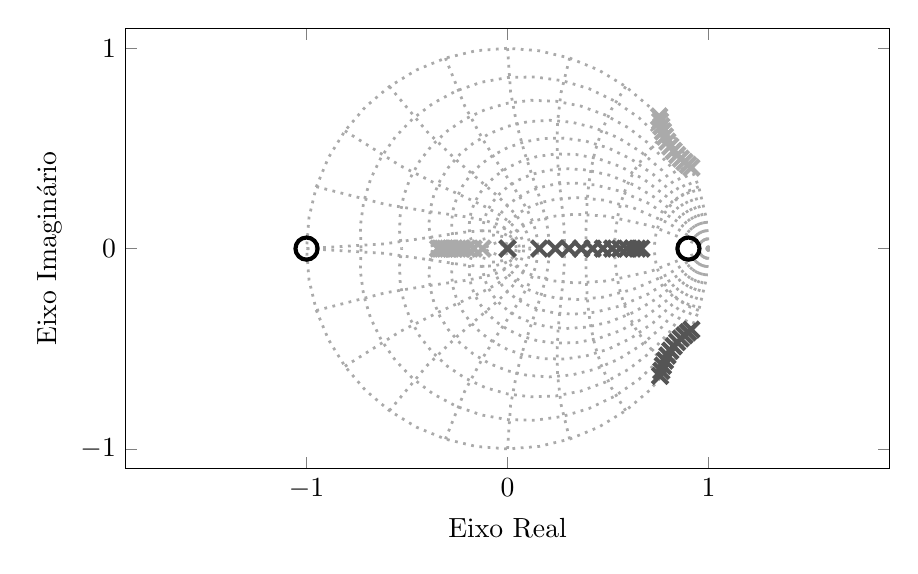
\begin{tikzpicture}

\begin{axis}[%
width=0.8\textwidth,
height=0.461611624834875\textwidth,
scale only axis,
xmin=-1.9,
xmax=1.9,
xtick={-1,  0,  1},
xlabel={Eixo Real},
ymin=-1.1,
ymax=1.1,
ytick={-1,  0,  1},
ylabel={Eixo Imaginário},
scaled y ticks = false,
y tick label style={/pgf/number format/.cd, fixed, fixed zerofill, precision=0},
scaled x ticks = false,
x tick label style={/pgf/number format/.cd, fixed, fixed zerofill, precision=0}
]
\addplot [color=mycolor1,dotted,line width=1.0pt,forget plot]
  table[row sep=crcr]{1	0\\
0.987688340595138	0.156434465040231\\
0.951056516295154	0.309016994374947\\
0.891006524188368	0.453990499739547\\
0.809016994374947	0.587785252292473\\
0.707106781186548	0.707106781186547\\
0.587785252292473	0.809016994374947\\
0.453990499739547	0.891006524188368\\
0.309016994374947	0.951056516295154\\
0.156434465040231	0.987688340595138\\
6.12323399573677e-17	1\\
-0.156434465040231	0.987688340595138\\
-0.309016994374947	0.951056516295154\\
-0.453990499739547	0.891006524188368\\
-0.587785252292473	0.809016994374947\\
-0.707106781186547	0.707106781186548\\
-0.809016994374947	0.587785252292473\\
-0.891006524188368	0.453990499739547\\
-0.951056516295154	0.309016994374948\\
-0.987688340595138	0.156434465040231\\
-1	1.22464679914735e-16\\
};
\addplot [color=mycolor1,dotted,line width=1.0pt,forget plot]
  table[row sep=crcr]{1	0\\
0.972218045703082	0.153984211042097\\
0.921496791140463	0.299412457456957\\
0.849791018366557	0.432990150609548\\
0.759508516401756	0.551815237548133\\
0.653437051516106	0.653437051516106\\
0.534664304371591	0.735902282058355\\
0.406492952796512	0.797787339572243\\
0.272353130096494	0.83821674479613\\
0.135714483753824	0.856867527364047\\
5.22899666167123e-17	0.853959960588124\\
-0.131496350792703	0.830235283991667\\
-0.255686250369537	0.786921363444393\\
-0.369756251949576	0.725687504552447\\
-0.47122811850853	0.648589862732789\\
-0.558009078759514	0.558009078759514\\
-0.628431083783263	0.456581908289041\\
-0.681278445058817	0.347128705949459\\
-0.715803538350409	0.232578668243255\\
-0.731730559897045	0.115894735197653\\
-0.729247614287671	8.9307075662324e-17\\
};
\addplot [color=mycolor1,dotted,line width=1.0pt,forget plot]
  table[row sep=crcr]{1	0\\
0.956521682769877	0.151498151383791\\
0.891982039736211	0.289822533396298\\
0.809292583610082	0.412355167436434\\
0.711634858347723	0.517032989000692\\
0.602364630186427	0.602364630186426\\
0.484917701774751	0.667431957639199\\
0.362719588349683	0.711877274647591\\
0.239101059900595	0.735877395777214\\
0.117221283062812	0.740106053489981\\
4.44354699422903e-17	0.725686295399261\\
-0.109940132237539	0.694134676438339\\
-0.210320240583588	0.647299141978847\\
-0.299240493845688	0.587292536894097\\
-0.375203754387119	0.516423664031337\\
-0.437127756959533	0.437127756959533\\
-0.484346224770267	0.351898130574443\\
-0.516599582217932	0.263220634338226\\
-0.534016141209622	0.173512362385299\\
-0.537084820159711	0.0850658786478001\\
-0.526620599330303	6.44924231334916e-17\\
};
\addplot [color=mycolor1,dotted,line width=1.0pt,forget plot]
  table[row sep=crcr]{1	0\\
0.940082788364644	0.148894486293864\\
0.86158608093073	0.279946287694513\\
0.768279786681378	0.391458103646313\\
0.663960650859636	0.482395649771645\\
0.552351927561387	0.552351927561387\\
0.437014383712816	0.601498696728173\\
0.321269860940431	0.630527604183869\\
0.208138182971344	0.640583459188477\\
0.100287778328637	0.633192112325829\\
3.73630739569174e-17	0.610185303761559\\
-0.0908532273476425	0.573624701779294\\
-0.170819110593797	0.525727164509449\\
-0.238861981883349	0.468793035010043\\
-0.294350736089166	0.40513903143051\\
-0.337037028702328	0.337037028702328\\
-0.367025664975262	0.266659754473976\\
-0.384738677688982	0.196034147687371\\
-0.390874612629551	0.127002860400749\\
-0.386364521398959	0.0611941284830315\\
-0.372326104926586	4.55967972637346e-17\\
};
\addplot [color=mycolor1,dotted,line width=1.0pt,forget plot]
  table[row sep=crcr]{1	0\\
0.922246029428501	0.146069421212559\\
0.829201462983264	0.269423887468404\\
0.725373165529273	0.369596088217499\\
0.614985835074999	0.446813363302878\\
0.501902475185001	0.501902475185001\\
0.38956496084428	0.536190168955128\\
0.280953750703967	0.551402782692681\\
0.178565395716864	0.549567778706978\\
0.0844061798404073	0.532919645815306\\
3.08495992433718e-17	0.50381218919366\\
-0.0735915548753502	0.464638791061534\\
-0.135739038566523	0.417761804348184\\
-0.186207014322272	0.365451842507638\\
-0.225110018726605	0.309837359892227\\
-0.252864584784672	0.252864584784672\\
-0.270139142845401	0.196267575756099\\
-0.277803443075876	0.141547924204336\\
-0.27687894570066	0.0899634229303457\\
-0.268491413422519	0.0425248622468694\\
-0.253826721980109	3.10848082611005e-17\\
};
\addplot [color=mycolor1,dotted,line width=1.0pt,forget plot]
  table[row sep=crcr]{1	0\\
0.902056570675584	0.142871725087523\\
0.793293726869509	0.257756756757911\\
0.678769666307395	0.345850419328459\\
0.562876391436159	0.408953636388562\\
0.449318435861499	0.449318435861499\\
0.341115747349381	0.469505547439701\\
0.24062663375655	0.472256359314945\\
0.149586755320764	0.460380694230177\\
0.069160331541479	0.436661148025441\\
2.47240337905553e-17	0.403774113610049\\
-0.057687904157153	0.364227092250654\\
-0.104075505986926	0.320311471399148\\
-0.139645446506012	0.274069620358657\\
-0.165124892040398	0.227274916024158\\
-0.18142315316863	0.18142315316863\\
-0.189574186252466	0.137733708524426\\
-0.190684892879101	0.0971588057560207\\
-0.185889806735969	0.0603992595374446\\
-0.176312467991919	0.0279251515651378\\
-0.16303353482158	1.99658496572927e-17\\
};
\addplot [color=mycolor1,dotted,line width=1.0pt,forget plot]
  table[row sep=crcr]{1	0\\
0.877921760602431	0.139049146701748\\
0.751411952540787	0.244148543365328\\
0.625732257688895	0.318826509862098\\
0.505011411193747	0.36691226736026\\
0.392341669548685	0.392341669548685\\
0.289890514921595	0.399000063654162\\
0.199020572856858	0.390599867100522\\
0.120411913496453	0.370589763847805\\
0.0541820486548744	0.34209199176291\\
1.88512313530119e-17	0.307863971328499\\
-0.042808222513439	0.270280479734772\\
-0.075164540154518	0.231332667812908\\
-0.0981551954909503	0.192640417840451\\
-0.112959067758674	0.155474818616317\\
-0.120787864504912	0.120787864504912\\
-0.122837744156894	0.0892468451742257\\
-0.120251626285951	0.0612712639357851\\
-0.114091236431876	0.0370704898842818\\
-0.105317799143806	0.0166807006736036\\
-0.0947802248421549	1.16072298975411e-17\\
};
\addplot [color=mycolor1,dotted,line width=1.0pt,forget plot]
  table[row sep=crcr]{1	0\\
0.84674396664984	0.134111069256013\\
0.698989566160914	0.227115477506975\\
0.561406498364893	0.286050898428465\\
0.437004973478602	0.317502698182059\\
0.327450698344114	0.327450698344114\\
0.233352139914598	0.321181666481713\\
0.154515499860225	0.303253743289057\\
0.0901653834921457	0.27750051639687\\
0.0391311034995635	0.247064063991275\\
1.31311479217367e-17	0.214447919692096\\
-0.0287598398096346	0.181582482159892\\
-0.0487044416812479	0.149896858349689\\
-0.0613430200940395	0.120392455675976\\
-0.06808779312177	0.0937148074575858\\
-0.0702211210616195	0.0702211210616195\\
-0.068876740220244	0.0500418809603846\\
-0.0650321343871793	0.0331355275052096\\
-0.0595094084547913	0.0193357789181307\\
-0.0529823745536039	0.00839158374073751\\
-0.0459879102602678	5.63189470997126e-18\\
};
\addplot [color=mycolor1,dotted,line width=1.0pt,forget plot]
  table[row sep=crcr]{1	0\\
0.801053465278425	0.126874404768154\\
0.625589539649299	0.203266363189334\\
0.475341369738971	0.242198525079547\\
0.350045057714404	0.254322621147605\\
0.24813777530853	0.24813777530853\\
0.167289292234614	0.230253957320141\\
0.104794333468008	0.205670459781722\\
0.0578515468028918	0.178048753195384\\
0.0237523524567972	0.149966451301199\\
7.54043881219821e-18	0.123144711070133\\
-0.0156239119173694	0.0986454975334405\\
-0.0250311775652273	0.0770380431086105\\
-0.0298254673925332	0.0585357756361869\\
-0.0313184856998208	0.0431061974937683\\
-0.0305568546459545	0.0305568546459545\\
-0.0283545570469435	0.0206007915573586\\
-0.0253272293454815	0.012904867916705\\
-0.021925762268643	0.00712411201600239\\
-0.0184675753156993	0.00292497658052826\\
-0.0151646198645466	1.85713031774033e-18\\
};
\addplot [color=mycolor1,dotted,line width=1.0pt,forget plot]
  table[row sep=crcr]{1	0\\
0.714110955679367	0.113104064044896\\
0.497161927717827	0.161537702532642\\
0.336758208677056	0.171586877647116\\
0.221075553032581	0.160620791180475\\
0.139705610200823	0.139705610200823\\
0.0839640345306934	0.115566579097864\\
0.0468885871776745	0.0920240337831981\\
0.0230753615892199	0.0710186604775083\\
0.00844586939409394	0.0533251206797082\\
2.39022368106624e-18	0.0390353150431684\\
-0.00441505277265522	0.0278755461307222\\
-0.00630567510971132	0.0194068724759343\\
-0.00669794782622876	0.0131454627690819\\
-0.0062698831862128	0.00862975386096949\\
-0.0054534525074872	0.0054534525074872\\
-0.00451117782354635	0.00327756254020109\\
-0.00359218715027031	0.00183031077240959\\
-0.00277223578568335	0.000900754009370227\\
-0.00208156288544739	0.000329687172611911\\
-0.00152375582051941	1.86606268828125e-19\\
};
\addplot [color=mycolor1,dotted,line width=1.0pt,forget plot]
  table[row sep=crcr]{1	-0\\
0.987688340595138	-0.156434465040231\\
0.951056516295154	-0.309016994374947\\
0.891006524188368	-0.453990499739547\\
0.809016994374947	-0.587785252292473\\
0.707106781186548	-0.707106781186547\\
0.587785252292473	-0.809016994374947\\
0.453990499739547	-0.891006524188368\\
0.309016994374947	-0.951056516295154\\
0.156434465040231	-0.987688340595138\\
6.12323399573677e-17	-1\\
-0.156434465040231	-0.987688340595138\\
-0.309016994374947	-0.951056516295154\\
-0.453990499739547	-0.891006524188368\\
-0.587785252292473	-0.809016994374947\\
-0.707106781186547	-0.707106781186548\\
-0.809016994374947	-0.587785252292473\\
-0.891006524188368	-0.453990499739547\\
-0.951056516295154	-0.309016994374948\\
-0.987688340595138	-0.156434465040231\\
-1	-1.22464679914735e-16\\
};
\addplot [color=mycolor1,dotted,line width=1.0pt,forget plot]
  table[row sep=crcr]{1	-0\\
0.972218045703082	-0.153984211042097\\
0.921496791140463	-0.299412457456957\\
0.849791018366557	-0.432990150609548\\
0.759508516401756	-0.551815237548133\\
0.653437051516106	-0.653437051516106\\
0.534664304371591	-0.735902282058355\\
0.406492952796512	-0.797787339572243\\
0.272353130096494	-0.83821674479613\\
0.135714483753824	-0.856867527364047\\
5.22899666167123e-17	-0.853959960588124\\
-0.131496350792703	-0.830235283991667\\
-0.255686250369537	-0.786921363444393\\
-0.369756251949576	-0.725687504552447\\
-0.47122811850853	-0.648589862732789\\
-0.558009078759514	-0.558009078759514\\
-0.628431083783263	-0.456581908289041\\
-0.681278445058817	-0.347128705949459\\
-0.715803538350409	-0.232578668243255\\
-0.731730559897045	-0.115894735197653\\
-0.729247614287671	-8.9307075662324e-17\\
};
\addplot [color=mycolor1,dotted,line width=1.0pt,forget plot]
  table[row sep=crcr]{1	-0\\
0.956521682769877	-0.151498151383791\\
0.891982039736211	-0.289822533396298\\
0.809292583610082	-0.412355167436434\\
0.711634858347723	-0.517032989000692\\
0.602364630186427	-0.602364630186426\\
0.484917701774751	-0.667431957639199\\
0.362719588349683	-0.711877274647591\\
0.239101059900595	-0.735877395777214\\
0.117221283062812	-0.740106053489981\\
4.44354699422903e-17	-0.725686295399261\\
-0.109940132237539	-0.694134676438339\\
-0.210320240583588	-0.647299141978847\\
-0.299240493845688	-0.587292536894097\\
-0.375203754387119	-0.516423664031337\\
-0.437127756959533	-0.437127756959533\\
-0.484346224770267	-0.351898130574443\\
-0.516599582217932	-0.263220634338226\\
-0.534016141209622	-0.173512362385299\\
-0.537084820159711	-0.0850658786478001\\
-0.526620599330303	-6.44924231334916e-17\\
};
\addplot [color=mycolor1,dotted,line width=1.0pt,forget plot]
  table[row sep=crcr]{1	-0\\
0.940082788364644	-0.148894486293864\\
0.86158608093073	-0.279946287694513\\
0.768279786681378	-0.391458103646313\\
0.663960650859636	-0.482395649771645\\
0.552351927561387	-0.552351927561387\\
0.437014383712816	-0.601498696728173\\
0.321269860940431	-0.630527604183869\\
0.208138182971344	-0.640583459188477\\
0.100287778328637	-0.633192112325829\\
3.73630739569174e-17	-0.610185303761559\\
-0.0908532273476425	-0.573624701779294\\
-0.170819110593797	-0.525727164509449\\
-0.238861981883349	-0.468793035010043\\
-0.294350736089166	-0.40513903143051\\
-0.337037028702328	-0.337037028702328\\
-0.367025664975262	-0.266659754473976\\
-0.384738677688982	-0.196034147687371\\
-0.390874612629551	-0.127002860400749\\
-0.386364521398959	-0.0611941284830315\\
-0.372326104926586	-4.55967972637346e-17\\
};
\addplot [color=mycolor1,dotted,line width=1.0pt,forget plot]
  table[row sep=crcr]{1	-0\\
0.922246029428501	-0.146069421212559\\
0.829201462983264	-0.269423887468404\\
0.725373165529273	-0.369596088217499\\
0.614985835074999	-0.446813363302878\\
0.501902475185001	-0.501902475185001\\
0.38956496084428	-0.536190168955128\\
0.280953750703967	-0.551402782692681\\
0.178565395716864	-0.549567778706978\\
0.0844061798404073	-0.532919645815306\\
3.08495992433718e-17	-0.50381218919366\\
-0.0735915548753502	-0.464638791061534\\
-0.135739038566523	-0.417761804348184\\
-0.186207014322272	-0.365451842507638\\
-0.225110018726605	-0.309837359892227\\
-0.252864584784672	-0.252864584784672\\
-0.270139142845401	-0.196267575756099\\
-0.277803443075876	-0.141547924204336\\
-0.27687894570066	-0.0899634229303457\\
-0.268491413422519	-0.0425248622468694\\
-0.253826721980109	-3.10848082611005e-17\\
};
\addplot [color=mycolor1,dotted,line width=1.0pt,forget plot]
  table[row sep=crcr]{1	-0\\
0.902056570675584	-0.142871725087523\\
0.793293726869509	-0.257756756757911\\
0.678769666307395	-0.345850419328459\\
0.562876391436159	-0.408953636388562\\
0.449318435861499	-0.449318435861499\\
0.341115747349381	-0.469505547439701\\
0.24062663375655	-0.472256359314945\\
0.149586755320764	-0.460380694230177\\
0.069160331541479	-0.436661148025441\\
2.47240337905553e-17	-0.403774113610049\\
-0.057687904157153	-0.364227092250654\\
-0.104075505986926	-0.320311471399148\\
-0.139645446506012	-0.274069620358657\\
-0.165124892040398	-0.227274916024158\\
-0.18142315316863	-0.18142315316863\\
-0.189574186252466	-0.137733708524426\\
-0.190684892879101	-0.0971588057560207\\
-0.185889806735969	-0.0603992595374446\\
-0.176312467991919	-0.0279251515651378\\
-0.16303353482158	-1.99658496572927e-17\\
};
\addplot [color=mycolor1,dotted,line width=1.0pt,forget plot]
  table[row sep=crcr]{1	-0\\
0.877921760602431	-0.139049146701748\\
0.751411952540787	-0.244148543365328\\
0.625732257688895	-0.318826509862098\\
0.505011411193747	-0.36691226736026\\
0.392341669548685	-0.392341669548685\\
0.289890514921595	-0.399000063654162\\
0.199020572856858	-0.390599867100522\\
0.120411913496453	-0.370589763847805\\
0.0541820486548744	-0.34209199176291\\
1.88512313530119e-17	-0.307863971328499\\
-0.042808222513439	-0.270280479734772\\
-0.075164540154518	-0.231332667812908\\
-0.0981551954909503	-0.192640417840451\\
-0.112959067758674	-0.155474818616317\\
-0.120787864504912	-0.120787864504912\\
-0.122837744156894	-0.0892468451742257\\
-0.120251626285951	-0.0612712639357851\\
-0.114091236431876	-0.0370704898842818\\
-0.105317799143806	-0.0166807006736036\\
-0.0947802248421549	-1.16072298975411e-17\\
};
\addplot [color=mycolor1,dotted,line width=1.0pt,forget plot]
  table[row sep=crcr]{1	-0\\
0.84674396664984	-0.134111069256013\\
0.698989566160914	-0.227115477506975\\
0.561406498364893	-0.286050898428465\\
0.437004973478602	-0.317502698182059\\
0.327450698344114	-0.327450698344114\\
0.233352139914598	-0.321181666481713\\
0.154515499860225	-0.303253743289057\\
0.0901653834921457	-0.27750051639687\\
0.0391311034995635	-0.247064063991275\\
1.31311479217367e-17	-0.214447919692096\\
-0.0287598398096346	-0.181582482159892\\
-0.0487044416812479	-0.149896858349689\\
-0.0613430200940395	-0.120392455675976\\
-0.06808779312177	-0.0937148074575858\\
-0.0702211210616195	-0.0702211210616195\\
-0.068876740220244	-0.0500418809603846\\
-0.0650321343871793	-0.0331355275052096\\
-0.0595094084547913	-0.0193357789181307\\
-0.0529823745536039	-0.00839158374073751\\
-0.0459879102602678	-5.63189470997126e-18\\
};
\addplot [color=mycolor1,dotted,line width=1.0pt,forget plot]
  table[row sep=crcr]{1	-0\\
0.801053465278425	-0.126874404768154\\
0.625589539649299	-0.203266363189334\\
0.475341369738971	-0.242198525079547\\
0.350045057714404	-0.254322621147605\\
0.24813777530853	-0.24813777530853\\
0.167289292234614	-0.230253957320141\\
0.104794333468008	-0.205670459781722\\
0.0578515468028918	-0.178048753195384\\
0.0237523524567972	-0.149966451301199\\
7.54043881219821e-18	-0.123144711070133\\
-0.0156239119173694	-0.0986454975334405\\
-0.0250311775652273	-0.0770380431086105\\
-0.0298254673925332	-0.0585357756361869\\
-0.0313184856998208	-0.0431061974937683\\
-0.0305568546459545	-0.0305568546459545\\
-0.0283545570469435	-0.0206007915573586\\
-0.0253272293454815	-0.012904867916705\\
-0.021925762268643	-0.00712411201600239\\
-0.0184675753156993	-0.00292497658052826\\
-0.0151646198645466	-1.85713031774033e-18\\
};
\addplot [color=mycolor1,dotted,line width=1.0pt,forget plot]
  table[row sep=crcr]{1	-0\\
0.714110955679367	-0.113104064044896\\
0.497161927717827	-0.161537702532642\\
0.336758208677056	-0.171586877647116\\
0.221075553032581	-0.160620791180475\\
0.139705610200823	-0.139705610200823\\
0.0839640345306934	-0.115566579097864\\
0.0468885871776745	-0.0920240337831981\\
0.0230753615892199	-0.0710186604775083\\
0.00844586939409394	-0.0533251206797082\\
2.39022368106624e-18	-0.0390353150431684\\
-0.00441505277265522	-0.0278755461307222\\
-0.00630567510971132	-0.0194068724759343\\
-0.00669794782622876	-0.0131454627690819\\
-0.0062698831862128	-0.00862975386096949\\
-0.0054534525074872	-0.0054534525074872\\
-0.00451117782354635	-0.00327756254020109\\
-0.00359218715027031	-0.00183031077240959\\
-0.00277223578568335	-0.000900754009370227\\
-0.00208156288544739	-0.000329687172611911\\
-0.00152375582051941	-1.86606268828125e-19\\
};
\addplot [color=mycolor1,dotted,line width=1.0pt,forget plot]
  table[row sep=crcr]{1	0\\
1	0\\
};
\addplot [color=mycolor1,dotted,line width=1.0pt,forget plot]
  table[row sep=crcr]{0.951056516295154	0.309016994374947\\
0.906577591518048	0.290693092532446\\
0.867277205719189	0.267124444629623\\
0.833330533437629	0.239553777474139\\
0.804679893747523	0.20903820245934\\
0.781122098933164	0.176433510213537\\
0.762382187756933	0.142402376999381\\
0.748171074803624	0.107437628337747\\
0.738227708485823	0.0718935522249012\\
0.732347931289196	0.0360204899377399\\
0.730402691048646	2.81010850277162e-17\\
};
\addplot [color=mycolor1,dotted,line width=1.0pt,forget plot]
  table[row sep=crcr]{0.809016994374947	0.587785252292473\\
0.737380455396588	0.527071687397996\\
0.6808142826414	0.463341883835339\\
0.637053765657314	0.399254954339046\\
0.603812761314093	0.336417677088311\\
0.579022949915482	0.275632227640288\\
0.560948163233974	0.217130071437151\\
0.54821711318997	0.160763451735608\\
0.539811466724715	0.106147624627789\\
0.535036016768209	0.0527590625798542\\
0.533488091091103	4.10502162512614e-17\\
};
\addplot [color=mycolor1,dotted,line width=1.0pt,forget plot]
  table[row sep=crcr]{0.587785252292473	0.809016994374947\\
0.515276498489902	0.692182785870847\\
0.46668476526979	0.583707991451876\\
0.435233321876477	0.485319980094308\\
0.415551842123536	0.396928474901319\\
0.403656860517901	0.317461475735791\\
0.396737049613855	0.245416450708029\\
0.392888142823216	0.179177710929467\\
0.39087245229983	0.11717008156476\\
0.389932112762627	0.0579102497954412\\
0.389661137375347	4.49747826270753e-17\\
};
\addplot [color=mycolor1,dotted,line width=1.0pt,forget plot]
  table[row sep=crcr]{0.309016994374947	0.951056516295154\\
0.265925372344309	0.777304721760365\\
0.248822386132444	0.630899544522142\\
0.24643298177389	0.508693744238057\\
0.251412997268255	0.406266573115132\\
0.25929445161488	0.31919477108011\\
0.267517373913267	0.243597429511063\\
0.274697115780397	0.1762665508339\\
0.280129101393366	0.114599409879343\\
0.283480020554887	0.0564559973822998\\
0.284609543336029	4.37996030135249e-17\\
};
\addplot [color=mycolor1,dotted,line width=1.0pt,forget plot]
  table[row sep=crcr]{6.12323399573677e-17	1\\
0.0151248701748503	0.781989711398728\\
0.0472692933177679	0.613631335769719\\
0.0835006201485716	0.482943980920436\\
0.117381749765263	0.379469463911326\\
0.146223972383669	0.295078319831894\\
0.169261627793672	0.223809451176491\\
0.186582776182006	0.161390341419992\\
0.198560105942714	0.104739935929793\\
0.205572433929556	0.0515565221197431\\
0.207879576350762	3.99891848849262e-17\\
};
\addplot [color=mycolor1,dotted,line width=1.0pt,forget plot]
  table[row sep=crcr]{-0.309016994374947	0.951056516295154\\
-0.213607139159912	0.713331044437031\\
-0.122920349149865	0.544815253953639\\
-0.0461074386071066	0.422454854218942\\
0.0151311193047769	0.329888717873058\\
0.0621570724668225	0.256291005261778\\
0.0971710522581798	0.194731597161215\\
0.122256440677152	0.140793596164787\\
0.13905244595299	0.0915971142347777\\
0.148693455532156	0.0451621321066958\\
0.151835801980649	3.50498499033503e-17\\
};
\addplot [color=mycolor1,dotted,line width=1.0pt,forget plot]
  table[row sep=crcr]{-0.587785252292473	0.809016994374948\\
-0.401011853057454	0.584595820351374\\
-0.252139489074835	0.439670821081765\\
-0.139623392550337	0.340999317931598\\
-0.0567836371213516	0.268617800427267\\
0.0033339412143336	0.21116115844769\\
0.0463512370945915	0.162297289886265\\
0.0763422025660035	0.118472638203443\\
0.0960671266193367	0.0776165020305757\\
0.1072685824301	0.0384304051397518\\
0.110901278364195	2.98672554719679e-17\\
};
\addplot [color=mycolor1,dotted,line width=1.0pt,forget plot]
  table[row sep=crcr]{-0.809016994374948	0.587785252292473\\
-0.533486326814499	0.413410095118228\\
-0.336121655437603	0.313963860155743\\
-0.198040110920963	0.250717832404618\\
-0.101844033235305	0.204281393673556\\
-0.0346516892466227	0.165530866251108\\
0.0122258376810533	0.130333089269644\\
0.0443886084751889	0.0968398262452624\\
0.065339288702761	0.0642052594194206\\
0.0771736424133687	0.032008294596762\\
0.0810025921579431	2.49315700239574e-17\\
};
\addplot [color=mycolor1,dotted,line width=1.0pt,forget plot]
  table[row sep=crcr]{-0.951056516295154	0.309016994374948\\
-0.60382220830535	0.219707538176049\\
-0.375378071887508	0.182507388795924\\
-0.225093275108467	0.161489568357552\\
-0.124654461172013	0.143091836517116\\
-0.0562723920172722	0.12318609851568\\
-0.00923898083522721	0.101104614081101\\
0.0228060316514889	0.0772217637055013\\
0.0436193292019494	0.0520955750986265\\
0.0553650029180358	0.0262210407420432\\
0.0591645112940776	2.0486346567262e-17\\
};
\addplot [color=mycolor1,dotted,line width=1.0pt,forget plot]
  table[row sep=crcr]{-1	1.22464679914735e-16\\
-0.61127914703566	0.0236549857259488\\
-0.374309030147768	0.0580118391989452\\
-0.226262535142082	0.0806522438077526\\
-0.130218598863194	0.0890855793127953\\
-0.0656897647351535	0.0862950481802363\\
-0.0214411717925588	0.0757647040434823\\
0.00876629006412298	0.0602253159022079\\
0.0284556614934045	0.0415943455493057\\
0.039601950618638	0.0211971994741971\\
0.0432139182637723	1.66258696249815e-17\\
};
\addplot [color=mycolor1,dotted,line width=1.0pt,forget plot]
  table[row sep=crcr]{1	-0\\
1	-0\\
};
\addplot [color=mycolor1,dotted,line width=1.0pt,forget plot]
  table[row sep=crcr]{0.951056516295154	-0.309016994374947\\
0.906577591518048	-0.290693092532446\\
0.867277205719189	-0.267124444629623\\
0.833330533437629	-0.239553777474139\\
0.804679893747523	-0.20903820245934\\
0.781122098933164	-0.176433510213537\\
0.762382187756933	-0.142402376999381\\
0.748171074803624	-0.107437628337747\\
0.738227708485823	-0.0718935522249012\\
0.732347931289196	-0.0360204899377399\\
0.730402691048646	-2.81010850277162e-17\\
};
\addplot [color=mycolor1,dotted,line width=1.0pt,forget plot]
  table[row sep=crcr]{0.809016994374947	-0.587785252292473\\
0.737380455396588	-0.527071687397996\\
0.6808142826414	-0.463341883835339\\
0.637053765657314	-0.399254954339046\\
0.603812761314093	-0.336417677088311\\
0.579022949915482	-0.275632227640288\\
0.560948163233974	-0.217130071437151\\
0.54821711318997	-0.160763451735608\\
0.539811466724715	-0.106147624627789\\
0.535036016768209	-0.0527590625798542\\
0.533488091091103	-4.10502162512614e-17\\
};
\addplot [color=mycolor1,dotted,line width=1.0pt,forget plot]
  table[row sep=crcr]{0.587785252292473	-0.809016994374947\\
0.515276498489902	-0.692182785870847\\
0.46668476526979	-0.583707991451876\\
0.435233321876477	-0.485319980094308\\
0.415551842123536	-0.396928474901319\\
0.403656860517901	-0.317461475735791\\
0.396737049613855	-0.245416450708029\\
0.392888142823216	-0.179177710929467\\
0.39087245229983	-0.11717008156476\\
0.389932112762627	-0.0579102497954412\\
0.389661137375347	-4.49747826270753e-17\\
};
\addplot [color=mycolor1,dotted,line width=1.0pt,forget plot]
  table[row sep=crcr]{0.309016994374947	-0.951056516295154\\
0.265925372344309	-0.777304721760365\\
0.248822386132444	-0.630899544522142\\
0.24643298177389	-0.508693744238057\\
0.251412997268255	-0.406266573115132\\
0.25929445161488	-0.31919477108011\\
0.267517373913267	-0.243597429511063\\
0.274697115780397	-0.1762665508339\\
0.280129101393366	-0.114599409879343\\
0.283480020554887	-0.0564559973822998\\
0.284609543336029	-4.37996030135249e-17\\
};
\addplot [color=mycolor1,dotted,line width=1.0pt,forget plot]
  table[row sep=crcr]{6.12323399573677e-17	-1\\
0.0151248701748503	-0.781989711398728\\
0.0472692933177679	-0.613631335769719\\
0.0835006201485716	-0.482943980920436\\
0.117381749765263	-0.379469463911326\\
0.146223972383669	-0.295078319831894\\
0.169261627793672	-0.223809451176491\\
0.186582776182006	-0.161390341419992\\
0.198560105942714	-0.104739935929793\\
0.205572433929556	-0.0515565221197431\\
0.207879576350762	-3.99891848849262e-17\\
};
\addplot [color=mycolor1,dotted,line width=1.0pt,forget plot]
  table[row sep=crcr]{-0.309016994374947	-0.951056516295154\\
-0.213607139159912	-0.713331044437031\\
-0.122920349149865	-0.544815253953639\\
-0.0461074386071066	-0.422454854218942\\
0.0151311193047769	-0.329888717873058\\
0.0621570724668225	-0.256291005261778\\
0.0971710522581798	-0.194731597161215\\
0.122256440677152	-0.140793596164787\\
0.13905244595299	-0.0915971142347777\\
0.148693455532156	-0.0451621321066958\\
0.151835801980649	-3.50498499033503e-17\\
};
\addplot [color=mycolor1,dotted,line width=1.0pt,forget plot]
  table[row sep=crcr]{-0.587785252292473	-0.809016994374948\\
-0.401011853057454	-0.584595820351374\\
-0.252139489074835	-0.439670821081765\\
-0.139623392550337	-0.340999317931598\\
-0.0567836371213516	-0.268617800427267\\
0.0033339412143336	-0.21116115844769\\
0.0463512370945915	-0.162297289886265\\
0.0763422025660035	-0.118472638203443\\
0.0960671266193367	-0.0776165020305757\\
0.1072685824301	-0.0384304051397518\\
0.110901278364195	-2.98672554719679e-17\\
};
\addplot [color=mycolor1,dotted,line width=1.0pt,forget plot]
  table[row sep=crcr]{-0.809016994374948	-0.587785252292473\\
-0.533486326814499	-0.413410095118228\\
-0.336121655437603	-0.313963860155743\\
-0.198040110920963	-0.250717832404618\\
-0.101844033235305	-0.204281393673556\\
-0.0346516892466227	-0.165530866251108\\
0.0122258376810533	-0.130333089269644\\
0.0443886084751889	-0.0968398262452624\\
0.065339288702761	-0.0642052594194206\\
0.0771736424133687	-0.032008294596762\\
0.0810025921579431	-2.49315700239574e-17\\
};
\addplot [color=mycolor1,dotted,line width=1.0pt,forget plot]
  table[row sep=crcr]{-0.951056516295154	-0.309016994374948\\
-0.60382220830535	-0.219707538176049\\
-0.375378071887508	-0.182507388795924\\
-0.225093275108467	-0.161489568357552\\
-0.124654461172013	-0.143091836517116\\
-0.0562723920172722	-0.12318609851568\\
-0.00923898083522721	-0.101104614081101\\
0.0228060316514889	-0.0772217637055013\\
0.0436193292019494	-0.0520955750986265\\
0.0553650029180358	-0.0262210407420432\\
0.0591645112940776	-2.0486346567262e-17\\
};
\addplot [color=mycolor1,dotted,line width=1.0pt,forget plot]
  table[row sep=crcr]{-1	-1.22464679914735e-16\\
-0.61127914703566	-0.0236549857259488\\
-0.374309030147768	-0.0580118391989452\\
-0.226262535142082	-0.0806522438077526\\
-0.130218598863194	-0.0890855793127953\\
-0.0656897647351535	-0.0862950481802363\\
-0.0214411717925588	-0.0757647040434823\\
0.00876629006412298	-0.0602253159022079\\
0.0284556614934045	-0.0415943455493057\\
0.039601950618638	-0.0211971994741971\\
0.0432139182637723	-1.66258696249815e-17\\
};
\addplot [color=mycolor1,line width=1.5pt,mark size=4.0pt,only marks,mark=x,mark options={solid},forget plot]
  table[row sep=crcr]{0	0\\
0.91444306659383	0.404714563561125\\
-0.124253880684544	0\\
0.89755799120607	0.418082106216459\\
-0.168612823306847	0\\
0.880031509804686	0.432694736532765\\
-0.20035214433653	0\\
0.862049033868094	0.448898382097043\\
-0.225714039094344	0\\
0.843968536244412	0.467035231637572\\
-0.247083156478973	0\\
0.826353726809843	0.487334319047914\\
-0.265667627304716	0\\
0.80991520639231	0.509761287368884\\
-0.28217711202824	0\\
0.795322964447454	0.533928890391685\\
-0.297069157418281	0\\
0.78298488576272	0.559181443716326\\
-0.310658437059747	0\\
0.772959683909908	0.584813903534905\\
-0.323171911393944	0\\
0.765041430382214	0.610258212917158\\
-0.334779380319558	0\\
0.758904835963185	0.635145159493358\\
-0.345611626818817	0\\
0.754213373942793	0.659276394587029\\
};
\addplot [color=black!50!mycolor1,line width=1.5pt,mark size=4.0pt,only marks,mark=x,mark options={solid},forget plot]
  table[row sep=crcr]{0	0\\
0.91444306659383	-0.404714563561125\\
0.158024031460067	0\\
0.89755799120607	-0.418082106216459\\
0.237435936885133	0\\
0.880031509804686	-0.432694736532765\\
0.305140209788	0\\
0.862049033868094	-0.448898382097043\\
0.36666309979318	0\\
0.843968536244412	-0.467035231637572\\
0.423261836046949	0\\
0.826353726809843	-0.487334319047914\\
0.474723347707758	0\\
0.80991520639231	-0.509761287368884\\
0.520417316320995	0\\
0.795322964447454	-0.533928890391685\\
0.559985519080503	0\\
0.78298488576272	-0.559181443716326\\
0.593625202427589	0\\
0.772959683909908	-0.584813903534905\\
0.621975183817178	0\\
0.765041430382214	-0.610258212917158\\
0.645855841580849	0\\
0.758904835963185	-0.635145159493358\\
0.666071012120892	0\\
};
\addplot [color=black,line width=1.5pt,mark size=4.0pt,only marks,mark=o,mark options={solid},forget plot]
  table[row sep=crcr]{-1	0\\
0.9	0\\
};
\end{axis}
\end{tikzpicture}%}
    \renewcommand\figurename{Fig.}
    \caption{Lugar das raízes para a função de transferência do controlador proporcional-derivativo.}
    \label{fig:rlocus_vc_2}
  \end{figure}

  A partir da Fig.~\ref{fig:rlocus_vc_2} se pode escolher $K_P+K_D = 3$ para máximo amortecimento, escolha que resulta em $K_P = 0,3$ e $K_D = 2,7$.


\subsection{Projeto para corrente do capacitor como variável intermediária}

  Considerando o controlador da malha interna $C_i(z)$ como sendo do tipo proporcional, sua expressão é dada por
  %
  \begin{equation}
    C_i(z) = K_P\text{.}
  \end{equation}

  Tendo como referência a função de transferência de malha fechada $I_C/U$, que pode ser vista na Fig.~\ref{fig:sistema_discreto} fazendo $U_p = I_C$, observa-se que sua equação característica é
  %
  \begin{equation}
    z^3 - 2 \cos \left( \omega_n T_s \right) z^2 + \left( 1 + K_P K_{id} \right) z - K_P K_{id} = 0\text{,}
    \label{eq:eq_caracteristica}
  \end{equation}
  %
  com
  %
  \begin{equation}
    K_{id} = \frac{\sin(\omega_n T_s)}{\omega_n L_1}\text{.}
  \end{equation}

  A transformação bilinear, dada por
  %
  \begin{equation}
    z = \frac{w + 1}{w - 1}\text{,}
  \end{equation}
  %
  mapeia o interior do círculo de raio unitário do plano $z$ no semiplano esquerdo do plano $w$. Aplicando a transformação bilinear à equação característica~(\ref{eq:eq_caracteristica}) se pode utilizar o critério de estabilidade de Routh-Hurwitz da mesma forma que se faria para um sistema em tempo contínuo~\cite{ref:OGATA}. Ou seja, se pode projetar o ganho $K_P$ como sendo
  %
  \begin{equation}
    \overline{K_P} = \frac{2 \cos \left( \omega_n T_s \right) - 1}
      {\sen \left( \omega_n T_s \right)} \omega_n L_1\text{,}
  \end{equation}
  %
  onde $\overline{K_P}$ representa o limite superior para o valor de $K_P$.

  \begin{figure}[htb]
    \centering{
      \def\svgwidth{\textwidth}
      % This file was created by matlab2tikz v0.4.7 running on MATLAB 7.14.
% Copyright (c) 2008--2014, Nico Schlömer <nico.schloemer@gmail.com>
% All rights reserved.
% Minimal pgfplots version: 1.3
% 
% The latest updates can be retrieved from
%   http://www.mathworks.com/matlabcentral/fileexchange/22022-matlab2tikz
% where you can also make suggestions and rate matlab2tikz.
% 
%
% defining custom colors
\definecolor{mycolor1}{rgb}{0.66667,0.66667,0.66667}%
%
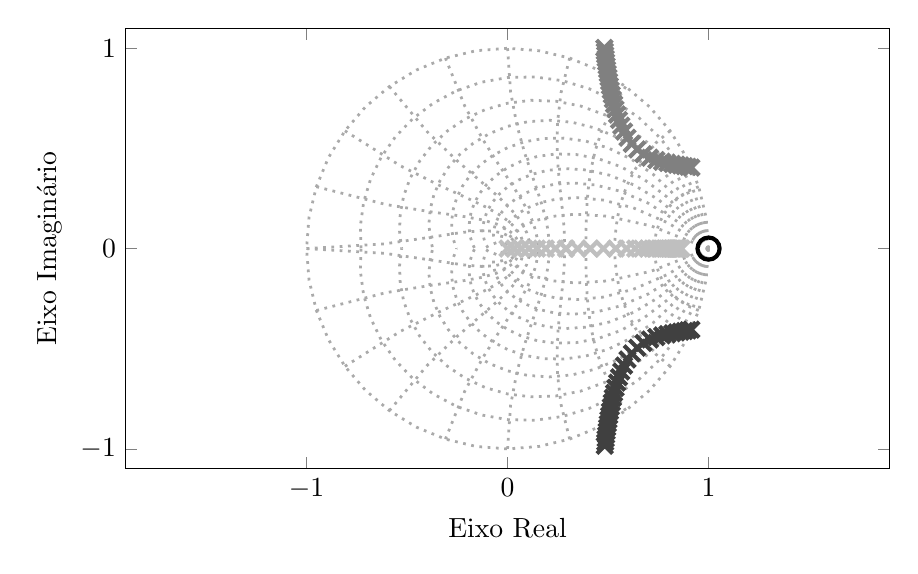
\begin{tikzpicture}

\begin{axis}[%
width=0.8\textwidth,
height=0.461611624834875\textwidth,
scale only axis,
xmin=-1.9,
xmax=1.9,
xtick={-1,  0,  1},
xlabel={Eixo Real},
ymin=-1.1,
ymax=1.1,
ytick={-1,  0,  1},
ylabel={Eixo Imaginário},
scaled y ticks = false,
y tick label style={/pgf/number format/.cd, fixed, fixed zerofill, precision=0},
scaled x ticks = false,
x tick label style={/pgf/number format/.cd, fixed, fixed zerofill, precision=0}
]
\addplot [color=mycolor1,dotted,line width=1.0pt,forget plot]
  table[row sep=crcr]{1	0\\
0.987688340595138	0.156434465040231\\
0.951056516295154	0.309016994374947\\
0.891006524188368	0.453990499739547\\
0.809016994374947	0.587785252292473\\
0.707106781186548	0.707106781186547\\
0.587785252292473	0.809016994374947\\
0.453990499739547	0.891006524188368\\
0.309016994374947	0.951056516295154\\
0.156434465040231	0.987688340595138\\
6.12323399573677e-17	1\\
-0.156434465040231	0.987688340595138\\
-0.309016994374947	0.951056516295154\\
-0.453990499739547	0.891006524188368\\
-0.587785252292473	0.809016994374947\\
-0.707106781186547	0.707106781186548\\
-0.809016994374947	0.587785252292473\\
-0.891006524188368	0.453990499739547\\
-0.951056516295154	0.309016994374948\\
-0.987688340595138	0.156434465040231\\
-1	1.22464679914735e-16\\
};
\addplot [color=mycolor1,dotted,line width=1.0pt,forget plot]
  table[row sep=crcr]{1	0\\
0.972218045703082	0.153984211042097\\
0.921496791140463	0.299412457456957\\
0.849791018366557	0.432990150609548\\
0.759508516401756	0.551815237548133\\
0.653437051516106	0.653437051516106\\
0.534664304371591	0.735902282058355\\
0.406492952796512	0.797787339572243\\
0.272353130096494	0.83821674479613\\
0.135714483753824	0.856867527364047\\
5.22899666167123e-17	0.853959960588124\\
-0.131496350792703	0.830235283991667\\
-0.255686250369537	0.786921363444393\\
-0.369756251949576	0.725687504552447\\
-0.47122811850853	0.648589862732789\\
-0.558009078759514	0.558009078759514\\
-0.628431083783263	0.456581908289041\\
-0.681278445058817	0.347128705949459\\
-0.715803538350409	0.232578668243255\\
-0.731730559897045	0.115894735197653\\
-0.729247614287671	8.9307075662324e-17\\
};
\addplot [color=mycolor1,dotted,line width=1.0pt,forget plot]
  table[row sep=crcr]{1	0\\
0.956521682769877	0.151498151383791\\
0.891982039736211	0.289822533396298\\
0.809292583610082	0.412355167436434\\
0.711634858347723	0.517032989000692\\
0.602364630186427	0.602364630186426\\
0.484917701774751	0.667431957639199\\
0.362719588349683	0.711877274647591\\
0.239101059900595	0.735877395777214\\
0.117221283062812	0.740106053489981\\
4.44354699422903e-17	0.725686295399261\\
-0.109940132237539	0.694134676438339\\
-0.210320240583588	0.647299141978847\\
-0.299240493845688	0.587292536894097\\
-0.375203754387119	0.516423664031337\\
-0.437127756959533	0.437127756959533\\
-0.484346224770267	0.351898130574443\\
-0.516599582217932	0.263220634338226\\
-0.534016141209622	0.173512362385299\\
-0.537084820159711	0.0850658786478001\\
-0.526620599330303	6.44924231334916e-17\\
};
\addplot [color=mycolor1,dotted,line width=1.0pt,forget plot]
  table[row sep=crcr]{1	0\\
0.940082788364644	0.148894486293864\\
0.86158608093073	0.279946287694513\\
0.768279786681378	0.391458103646313\\
0.663960650859636	0.482395649771645\\
0.552351927561387	0.552351927561387\\
0.437014383712816	0.601498696728173\\
0.321269860940431	0.630527604183869\\
0.208138182971344	0.640583459188477\\
0.100287778328637	0.633192112325829\\
3.73630739569174e-17	0.610185303761559\\
-0.0908532273476425	0.573624701779294\\
-0.170819110593797	0.525727164509449\\
-0.238861981883349	0.468793035010043\\
-0.294350736089166	0.40513903143051\\
-0.337037028702328	0.337037028702328\\
-0.367025664975262	0.266659754473976\\
-0.384738677688982	0.196034147687371\\
-0.390874612629551	0.127002860400749\\
-0.386364521398959	0.0611941284830315\\
-0.372326104926586	4.55967972637346e-17\\
};
\addplot [color=mycolor1,dotted,line width=1.0pt,forget plot]
  table[row sep=crcr]{1	0\\
0.922246029428501	0.146069421212559\\
0.829201462983264	0.269423887468404\\
0.725373165529273	0.369596088217499\\
0.614985835074999	0.446813363302878\\
0.501902475185001	0.501902475185001\\
0.38956496084428	0.536190168955128\\
0.280953750703967	0.551402782692681\\
0.178565395716864	0.549567778706978\\
0.0844061798404073	0.532919645815306\\
3.08495992433718e-17	0.50381218919366\\
-0.0735915548753502	0.464638791061534\\
-0.135739038566523	0.417761804348184\\
-0.186207014322272	0.365451842507638\\
-0.225110018726605	0.309837359892227\\
-0.252864584784672	0.252864584784672\\
-0.270139142845401	0.196267575756099\\
-0.277803443075876	0.141547924204336\\
-0.27687894570066	0.0899634229303457\\
-0.268491413422519	0.0425248622468694\\
-0.253826721980109	3.10848082611005e-17\\
};
\addplot [color=mycolor1,dotted,line width=1.0pt,forget plot]
  table[row sep=crcr]{1	0\\
0.902056570675584	0.142871725087523\\
0.793293726869509	0.257756756757911\\
0.678769666307395	0.345850419328459\\
0.562876391436159	0.408953636388562\\
0.449318435861499	0.449318435861499\\
0.341115747349381	0.469505547439701\\
0.24062663375655	0.472256359314945\\
0.149586755320764	0.460380694230177\\
0.069160331541479	0.436661148025441\\
2.47240337905553e-17	0.403774113610049\\
-0.057687904157153	0.364227092250654\\
-0.104075505986926	0.320311471399148\\
-0.139645446506012	0.274069620358657\\
-0.165124892040398	0.227274916024158\\
-0.18142315316863	0.18142315316863\\
-0.189574186252466	0.137733708524426\\
-0.190684892879101	0.0971588057560207\\
-0.185889806735969	0.0603992595374446\\
-0.176312467991919	0.0279251515651378\\
-0.16303353482158	1.99658496572927e-17\\
};
\addplot [color=mycolor1,dotted,line width=1.0pt,forget plot]
  table[row sep=crcr]{1	0\\
0.877921760602431	0.139049146701748\\
0.751411952540787	0.244148543365328\\
0.625732257688895	0.318826509862098\\
0.505011411193747	0.36691226736026\\
0.392341669548685	0.392341669548685\\
0.289890514921595	0.399000063654162\\
0.199020572856858	0.390599867100522\\
0.120411913496453	0.370589763847805\\
0.0541820486548744	0.34209199176291\\
1.88512313530119e-17	0.307863971328499\\
-0.042808222513439	0.270280479734772\\
-0.075164540154518	0.231332667812908\\
-0.0981551954909503	0.192640417840451\\
-0.112959067758674	0.155474818616317\\
-0.120787864504912	0.120787864504912\\
-0.122837744156894	0.0892468451742257\\
-0.120251626285951	0.0612712639357851\\
-0.114091236431876	0.0370704898842818\\
-0.105317799143806	0.0166807006736036\\
-0.0947802248421549	1.16072298975411e-17\\
};
\addplot [color=mycolor1,dotted,line width=1.0pt,forget plot]
  table[row sep=crcr]{1	0\\
0.84674396664984	0.134111069256013\\
0.698989566160914	0.227115477506975\\
0.561406498364893	0.286050898428465\\
0.437004973478602	0.317502698182059\\
0.327450698344114	0.327450698344114\\
0.233352139914598	0.321181666481713\\
0.154515499860225	0.303253743289057\\
0.0901653834921457	0.27750051639687\\
0.0391311034995635	0.247064063991275\\
1.31311479217367e-17	0.214447919692096\\
-0.0287598398096346	0.181582482159892\\
-0.0487044416812479	0.149896858349689\\
-0.0613430200940395	0.120392455675976\\
-0.06808779312177	0.0937148074575858\\
-0.0702211210616195	0.0702211210616195\\
-0.068876740220244	0.0500418809603846\\
-0.0650321343871793	0.0331355275052096\\
-0.0595094084547913	0.0193357789181307\\
-0.0529823745536039	0.00839158374073751\\
-0.0459879102602678	5.63189470997126e-18\\
};
\addplot [color=mycolor1,dotted,line width=1.0pt,forget plot]
  table[row sep=crcr]{1	0\\
0.801053465278425	0.126874404768154\\
0.625589539649299	0.203266363189334\\
0.475341369738971	0.242198525079547\\
0.350045057714404	0.254322621147605\\
0.24813777530853	0.24813777530853\\
0.167289292234614	0.230253957320141\\
0.104794333468008	0.205670459781722\\
0.0578515468028918	0.178048753195384\\
0.0237523524567972	0.149966451301199\\
7.54043881219821e-18	0.123144711070133\\
-0.0156239119173694	0.0986454975334405\\
-0.0250311775652273	0.0770380431086105\\
-0.0298254673925332	0.0585357756361869\\
-0.0313184856998208	0.0431061974937683\\
-0.0305568546459545	0.0305568546459545\\
-0.0283545570469435	0.0206007915573586\\
-0.0253272293454815	0.012904867916705\\
-0.021925762268643	0.00712411201600239\\
-0.0184675753156993	0.00292497658052826\\
-0.0151646198645466	1.85713031774033e-18\\
};
\addplot [color=mycolor1,dotted,line width=1.0pt,forget plot]
  table[row sep=crcr]{1	0\\
0.714110955679367	0.113104064044896\\
0.497161927717827	0.161537702532642\\
0.336758208677056	0.171586877647116\\
0.221075553032581	0.160620791180475\\
0.139705610200823	0.139705610200823\\
0.0839640345306934	0.115566579097864\\
0.0468885871776745	0.0920240337831981\\
0.0230753615892199	0.0710186604775083\\
0.00844586939409394	0.0533251206797082\\
2.39022368106624e-18	0.0390353150431684\\
-0.00441505277265522	0.0278755461307222\\
-0.00630567510971132	0.0194068724759343\\
-0.00669794782622876	0.0131454627690819\\
-0.0062698831862128	0.00862975386096949\\
-0.0054534525074872	0.0054534525074872\\
-0.00451117782354635	0.00327756254020109\\
-0.00359218715027031	0.00183031077240959\\
-0.00277223578568335	0.000900754009370227\\
-0.00208156288544739	0.000329687172611911\\
-0.00152375582051941	1.86606268828125e-19\\
};
\addplot [color=mycolor1,dotted,line width=1.0pt,forget plot]
  table[row sep=crcr]{1	-0\\
0.987688340595138	-0.156434465040231\\
0.951056516295154	-0.309016994374947\\
0.891006524188368	-0.453990499739547\\
0.809016994374947	-0.587785252292473\\
0.707106781186548	-0.707106781186547\\
0.587785252292473	-0.809016994374947\\
0.453990499739547	-0.891006524188368\\
0.309016994374947	-0.951056516295154\\
0.156434465040231	-0.987688340595138\\
6.12323399573677e-17	-1\\
-0.156434465040231	-0.987688340595138\\
-0.309016994374947	-0.951056516295154\\
-0.453990499739547	-0.891006524188368\\
-0.587785252292473	-0.809016994374947\\
-0.707106781186547	-0.707106781186548\\
-0.809016994374947	-0.587785252292473\\
-0.891006524188368	-0.453990499739547\\
-0.951056516295154	-0.309016994374948\\
-0.987688340595138	-0.156434465040231\\
-1	-1.22464679914735e-16\\
};
\addplot [color=mycolor1,dotted,line width=1.0pt,forget plot]
  table[row sep=crcr]{1	-0\\
0.972218045703082	-0.153984211042097\\
0.921496791140463	-0.299412457456957\\
0.849791018366557	-0.432990150609548\\
0.759508516401756	-0.551815237548133\\
0.653437051516106	-0.653437051516106\\
0.534664304371591	-0.735902282058355\\
0.406492952796512	-0.797787339572243\\
0.272353130096494	-0.83821674479613\\
0.135714483753824	-0.856867527364047\\
5.22899666167123e-17	-0.853959960588124\\
-0.131496350792703	-0.830235283991667\\
-0.255686250369537	-0.786921363444393\\
-0.369756251949576	-0.725687504552447\\
-0.47122811850853	-0.648589862732789\\
-0.558009078759514	-0.558009078759514\\
-0.628431083783263	-0.456581908289041\\
-0.681278445058817	-0.347128705949459\\
-0.715803538350409	-0.232578668243255\\
-0.731730559897045	-0.115894735197653\\
-0.729247614287671	-8.9307075662324e-17\\
};
\addplot [color=mycolor1,dotted,line width=1.0pt,forget plot]
  table[row sep=crcr]{1	-0\\
0.956521682769877	-0.151498151383791\\
0.891982039736211	-0.289822533396298\\
0.809292583610082	-0.412355167436434\\
0.711634858347723	-0.517032989000692\\
0.602364630186427	-0.602364630186426\\
0.484917701774751	-0.667431957639199\\
0.362719588349683	-0.711877274647591\\
0.239101059900595	-0.735877395777214\\
0.117221283062812	-0.740106053489981\\
4.44354699422903e-17	-0.725686295399261\\
-0.109940132237539	-0.694134676438339\\
-0.210320240583588	-0.647299141978847\\
-0.299240493845688	-0.587292536894097\\
-0.375203754387119	-0.516423664031337\\
-0.437127756959533	-0.437127756959533\\
-0.484346224770267	-0.351898130574443\\
-0.516599582217932	-0.263220634338226\\
-0.534016141209622	-0.173512362385299\\
-0.537084820159711	-0.0850658786478001\\
-0.526620599330303	-6.44924231334916e-17\\
};
\addplot [color=mycolor1,dotted,line width=1.0pt,forget plot]
  table[row sep=crcr]{1	-0\\
0.940082788364644	-0.148894486293864\\
0.86158608093073	-0.279946287694513\\
0.768279786681378	-0.391458103646313\\
0.663960650859636	-0.482395649771645\\
0.552351927561387	-0.552351927561387\\
0.437014383712816	-0.601498696728173\\
0.321269860940431	-0.630527604183869\\
0.208138182971344	-0.640583459188477\\
0.100287778328637	-0.633192112325829\\
3.73630739569174e-17	-0.610185303761559\\
-0.0908532273476425	-0.573624701779294\\
-0.170819110593797	-0.525727164509449\\
-0.238861981883349	-0.468793035010043\\
-0.294350736089166	-0.40513903143051\\
-0.337037028702328	-0.337037028702328\\
-0.367025664975262	-0.266659754473976\\
-0.384738677688982	-0.196034147687371\\
-0.390874612629551	-0.127002860400749\\
-0.386364521398959	-0.0611941284830315\\
-0.372326104926586	-4.55967972637346e-17\\
};
\addplot [color=mycolor1,dotted,line width=1.0pt,forget plot]
  table[row sep=crcr]{1	-0\\
0.922246029428501	-0.146069421212559\\
0.829201462983264	-0.269423887468404\\
0.725373165529273	-0.369596088217499\\
0.614985835074999	-0.446813363302878\\
0.501902475185001	-0.501902475185001\\
0.38956496084428	-0.536190168955128\\
0.280953750703967	-0.551402782692681\\
0.178565395716864	-0.549567778706978\\
0.0844061798404073	-0.532919645815306\\
3.08495992433718e-17	-0.50381218919366\\
-0.0735915548753502	-0.464638791061534\\
-0.135739038566523	-0.417761804348184\\
-0.186207014322272	-0.365451842507638\\
-0.225110018726605	-0.309837359892227\\
-0.252864584784672	-0.252864584784672\\
-0.270139142845401	-0.196267575756099\\
-0.277803443075876	-0.141547924204336\\
-0.27687894570066	-0.0899634229303457\\
-0.268491413422519	-0.0425248622468694\\
-0.253826721980109	-3.10848082611005e-17\\
};
\addplot [color=mycolor1,dotted,line width=1.0pt,forget plot]
  table[row sep=crcr]{1	-0\\
0.902056570675584	-0.142871725087523\\
0.793293726869509	-0.257756756757911\\
0.678769666307395	-0.345850419328459\\
0.562876391436159	-0.408953636388562\\
0.449318435861499	-0.449318435861499\\
0.341115747349381	-0.469505547439701\\
0.24062663375655	-0.472256359314945\\
0.149586755320764	-0.460380694230177\\
0.069160331541479	-0.436661148025441\\
2.47240337905553e-17	-0.403774113610049\\
-0.057687904157153	-0.364227092250654\\
-0.104075505986926	-0.320311471399148\\
-0.139645446506012	-0.274069620358657\\
-0.165124892040398	-0.227274916024158\\
-0.18142315316863	-0.18142315316863\\
-0.189574186252466	-0.137733708524426\\
-0.190684892879101	-0.0971588057560207\\
-0.185889806735969	-0.0603992595374446\\
-0.176312467991919	-0.0279251515651378\\
-0.16303353482158	-1.99658496572927e-17\\
};
\addplot [color=mycolor1,dotted,line width=1.0pt,forget plot]
  table[row sep=crcr]{1	-0\\
0.877921760602431	-0.139049146701748\\
0.751411952540787	-0.244148543365328\\
0.625732257688895	-0.318826509862098\\
0.505011411193747	-0.36691226736026\\
0.392341669548685	-0.392341669548685\\
0.289890514921595	-0.399000063654162\\
0.199020572856858	-0.390599867100522\\
0.120411913496453	-0.370589763847805\\
0.0541820486548744	-0.34209199176291\\
1.88512313530119e-17	-0.307863971328499\\
-0.042808222513439	-0.270280479734772\\
-0.075164540154518	-0.231332667812908\\
-0.0981551954909503	-0.192640417840451\\
-0.112959067758674	-0.155474818616317\\
-0.120787864504912	-0.120787864504912\\
-0.122837744156894	-0.0892468451742257\\
-0.120251626285951	-0.0612712639357851\\
-0.114091236431876	-0.0370704898842818\\
-0.105317799143806	-0.0166807006736036\\
-0.0947802248421549	-1.16072298975411e-17\\
};
\addplot [color=mycolor1,dotted,line width=1.0pt,forget plot]
  table[row sep=crcr]{1	-0\\
0.84674396664984	-0.134111069256013\\
0.698989566160914	-0.227115477506975\\
0.561406498364893	-0.286050898428465\\
0.437004973478602	-0.317502698182059\\
0.327450698344114	-0.327450698344114\\
0.233352139914598	-0.321181666481713\\
0.154515499860225	-0.303253743289057\\
0.0901653834921457	-0.27750051639687\\
0.0391311034995635	-0.247064063991275\\
1.31311479217367e-17	-0.214447919692096\\
-0.0287598398096346	-0.181582482159892\\
-0.0487044416812479	-0.149896858349689\\
-0.0613430200940395	-0.120392455675976\\
-0.06808779312177	-0.0937148074575858\\
-0.0702211210616195	-0.0702211210616195\\
-0.068876740220244	-0.0500418809603846\\
-0.0650321343871793	-0.0331355275052096\\
-0.0595094084547913	-0.0193357789181307\\
-0.0529823745536039	-0.00839158374073751\\
-0.0459879102602678	-5.63189470997126e-18\\
};
\addplot [color=mycolor1,dotted,line width=1.0pt,forget plot]
  table[row sep=crcr]{1	-0\\
0.801053465278425	-0.126874404768154\\
0.625589539649299	-0.203266363189334\\
0.475341369738971	-0.242198525079547\\
0.350045057714404	-0.254322621147605\\
0.24813777530853	-0.24813777530853\\
0.167289292234614	-0.230253957320141\\
0.104794333468008	-0.205670459781722\\
0.0578515468028918	-0.178048753195384\\
0.0237523524567972	-0.149966451301199\\
7.54043881219821e-18	-0.123144711070133\\
-0.0156239119173694	-0.0986454975334405\\
-0.0250311775652273	-0.0770380431086105\\
-0.0298254673925332	-0.0585357756361869\\
-0.0313184856998208	-0.0431061974937683\\
-0.0305568546459545	-0.0305568546459545\\
-0.0283545570469435	-0.0206007915573586\\
-0.0253272293454815	-0.012904867916705\\
-0.021925762268643	-0.00712411201600239\\
-0.0184675753156993	-0.00292497658052826\\
-0.0151646198645466	-1.85713031774033e-18\\
};
\addplot [color=mycolor1,dotted,line width=1.0pt,forget plot]
  table[row sep=crcr]{1	-0\\
0.714110955679367	-0.113104064044896\\
0.497161927717827	-0.161537702532642\\
0.336758208677056	-0.171586877647116\\
0.221075553032581	-0.160620791180475\\
0.139705610200823	-0.139705610200823\\
0.0839640345306934	-0.115566579097864\\
0.0468885871776745	-0.0920240337831981\\
0.0230753615892199	-0.0710186604775083\\
0.00844586939409394	-0.0533251206797082\\
2.39022368106624e-18	-0.0390353150431684\\
-0.00441505277265522	-0.0278755461307222\\
-0.00630567510971132	-0.0194068724759343\\
-0.00669794782622876	-0.0131454627690819\\
-0.0062698831862128	-0.00862975386096949\\
-0.0054534525074872	-0.0054534525074872\\
-0.00451117782354635	-0.00327756254020109\\
-0.00359218715027031	-0.00183031077240959\\
-0.00277223578568335	-0.000900754009370227\\
-0.00208156288544739	-0.000329687172611911\\
-0.00152375582051941	-1.86606268828125e-19\\
};
\addplot [color=mycolor1,dotted,line width=1.0pt,forget plot]
  table[row sep=crcr]{1	0\\
1	0\\
};
\addplot [color=mycolor1,dotted,line width=1.0pt,forget plot]
  table[row sep=crcr]{0.951056516295154	0.309016994374947\\
0.906577591518048	0.290693092532446\\
0.867277205719189	0.267124444629623\\
0.833330533437629	0.239553777474139\\
0.804679893747523	0.20903820245934\\
0.781122098933164	0.176433510213537\\
0.762382187756933	0.142402376999381\\
0.748171074803624	0.107437628337747\\
0.738227708485823	0.0718935522249012\\
0.732347931289196	0.0360204899377399\\
0.730402691048646	2.81010850277162e-17\\
};
\addplot [color=mycolor1,dotted,line width=1.0pt,forget plot]
  table[row sep=crcr]{0.809016994374947	0.587785252292473\\
0.737380455396588	0.527071687397996\\
0.6808142826414	0.463341883835339\\
0.637053765657314	0.399254954339046\\
0.603812761314093	0.336417677088311\\
0.579022949915482	0.275632227640288\\
0.560948163233974	0.217130071437151\\
0.54821711318997	0.160763451735608\\
0.539811466724715	0.106147624627789\\
0.535036016768209	0.0527590625798542\\
0.533488091091103	4.10502162512614e-17\\
};
\addplot [color=mycolor1,dotted,line width=1.0pt,forget plot]
  table[row sep=crcr]{0.587785252292473	0.809016994374947\\
0.515276498489902	0.692182785870847\\
0.46668476526979	0.583707991451876\\
0.435233321876477	0.485319980094308\\
0.415551842123536	0.396928474901319\\
0.403656860517901	0.317461475735791\\
0.396737049613855	0.245416450708029\\
0.392888142823216	0.179177710929467\\
0.39087245229983	0.11717008156476\\
0.389932112762627	0.0579102497954412\\
0.389661137375347	4.49747826270753e-17\\
};
\addplot [color=mycolor1,dotted,line width=1.0pt,forget plot]
  table[row sep=crcr]{0.309016994374947	0.951056516295154\\
0.265925372344309	0.777304721760365\\
0.248822386132444	0.630899544522142\\
0.24643298177389	0.508693744238057\\
0.251412997268255	0.406266573115132\\
0.25929445161488	0.31919477108011\\
0.267517373913267	0.243597429511063\\
0.274697115780397	0.1762665508339\\
0.280129101393366	0.114599409879343\\
0.283480020554887	0.0564559973822998\\
0.284609543336029	4.37996030135249e-17\\
};
\addplot [color=mycolor1,dotted,line width=1.0pt,forget plot]
  table[row sep=crcr]{6.12323399573677e-17	1\\
0.0151248701748503	0.781989711398728\\
0.0472692933177679	0.613631335769719\\
0.0835006201485716	0.482943980920436\\
0.117381749765263	0.379469463911326\\
0.146223972383669	0.295078319831894\\
0.169261627793672	0.223809451176491\\
0.186582776182006	0.161390341419992\\
0.198560105942714	0.104739935929793\\
0.205572433929556	0.0515565221197431\\
0.207879576350762	3.99891848849262e-17\\
};
\addplot [color=mycolor1,dotted,line width=1.0pt,forget plot]
  table[row sep=crcr]{-0.309016994374947	0.951056516295154\\
-0.213607139159912	0.713331044437031\\
-0.122920349149865	0.544815253953639\\
-0.0461074386071066	0.422454854218942\\
0.0151311193047769	0.329888717873058\\
0.0621570724668225	0.256291005261778\\
0.0971710522581798	0.194731597161215\\
0.122256440677152	0.140793596164787\\
0.13905244595299	0.0915971142347777\\
0.148693455532156	0.0451621321066958\\
0.151835801980649	3.50498499033503e-17\\
};
\addplot [color=mycolor1,dotted,line width=1.0pt,forget plot]
  table[row sep=crcr]{-0.587785252292473	0.809016994374948\\
-0.401011853057454	0.584595820351374\\
-0.252139489074835	0.439670821081765\\
-0.139623392550337	0.340999317931598\\
-0.0567836371213516	0.268617800427267\\
0.0033339412143336	0.21116115844769\\
0.0463512370945915	0.162297289886265\\
0.0763422025660035	0.118472638203443\\
0.0960671266193367	0.0776165020305757\\
0.1072685824301	0.0384304051397518\\
0.110901278364195	2.98672554719679e-17\\
};
\addplot [color=mycolor1,dotted,line width=1.0pt,forget plot]
  table[row sep=crcr]{-0.809016994374948	0.587785252292473\\
-0.533486326814499	0.413410095118228\\
-0.336121655437603	0.313963860155743\\
-0.198040110920963	0.250717832404618\\
-0.101844033235305	0.204281393673556\\
-0.0346516892466227	0.165530866251108\\
0.0122258376810533	0.130333089269644\\
0.0443886084751889	0.0968398262452624\\
0.065339288702761	0.0642052594194206\\
0.0771736424133687	0.032008294596762\\
0.0810025921579431	2.49315700239574e-17\\
};
\addplot [color=mycolor1,dotted,line width=1.0pt,forget plot]
  table[row sep=crcr]{-0.951056516295154	0.309016994374948\\
-0.60382220830535	0.219707538176049\\
-0.375378071887508	0.182507388795924\\
-0.225093275108467	0.161489568357552\\
-0.124654461172013	0.143091836517116\\
-0.0562723920172722	0.12318609851568\\
-0.00923898083522721	0.101104614081101\\
0.0228060316514889	0.0772217637055013\\
0.0436193292019494	0.0520955750986265\\
0.0553650029180358	0.0262210407420432\\
0.0591645112940776	2.0486346567262e-17\\
};
\addplot [color=mycolor1,dotted,line width=1.0pt,forget plot]
  table[row sep=crcr]{-1	1.22464679914735e-16\\
-0.61127914703566	0.0236549857259488\\
-0.374309030147768	0.0580118391989452\\
-0.226262535142082	0.0806522438077526\\
-0.130218598863194	0.0890855793127953\\
-0.0656897647351535	0.0862950481802363\\
-0.0214411717925588	0.0757647040434823\\
0.00876629006412298	0.0602253159022079\\
0.0284556614934045	0.0415943455493057\\
0.039601950618638	0.0211971994741971\\
0.0432139182637723	1.66258696249815e-17\\
};
\addplot [color=mycolor1,dotted,line width=1.0pt,forget plot]
  table[row sep=crcr]{1	-0\\
1	-0\\
};
\addplot [color=mycolor1,dotted,line width=1.0pt,forget plot]
  table[row sep=crcr]{0.951056516295154	-0.309016994374947\\
0.906577591518048	-0.290693092532446\\
0.867277205719189	-0.267124444629623\\
0.833330533437629	-0.239553777474139\\
0.804679893747523	-0.20903820245934\\
0.781122098933164	-0.176433510213537\\
0.762382187756933	-0.142402376999381\\
0.748171074803624	-0.107437628337747\\
0.738227708485823	-0.0718935522249012\\
0.732347931289196	-0.0360204899377399\\
0.730402691048646	-2.81010850277162e-17\\
};
\addplot [color=mycolor1,dotted,line width=1.0pt,forget plot]
  table[row sep=crcr]{0.809016994374947	-0.587785252292473\\
0.737380455396588	-0.527071687397996\\
0.6808142826414	-0.463341883835339\\
0.637053765657314	-0.399254954339046\\
0.603812761314093	-0.336417677088311\\
0.579022949915482	-0.275632227640288\\
0.560948163233974	-0.217130071437151\\
0.54821711318997	-0.160763451735608\\
0.539811466724715	-0.106147624627789\\
0.535036016768209	-0.0527590625798542\\
0.533488091091103	-4.10502162512614e-17\\
};
\addplot [color=mycolor1,dotted,line width=1.0pt,forget plot]
  table[row sep=crcr]{0.587785252292473	-0.809016994374947\\
0.515276498489902	-0.692182785870847\\
0.46668476526979	-0.583707991451876\\
0.435233321876477	-0.485319980094308\\
0.415551842123536	-0.396928474901319\\
0.403656860517901	-0.317461475735791\\
0.396737049613855	-0.245416450708029\\
0.392888142823216	-0.179177710929467\\
0.39087245229983	-0.11717008156476\\
0.389932112762627	-0.0579102497954412\\
0.389661137375347	-4.49747826270753e-17\\
};
\addplot [color=mycolor1,dotted,line width=1.0pt,forget plot]
  table[row sep=crcr]{0.309016994374947	-0.951056516295154\\
0.265925372344309	-0.777304721760365\\
0.248822386132444	-0.630899544522142\\
0.24643298177389	-0.508693744238057\\
0.251412997268255	-0.406266573115132\\
0.25929445161488	-0.31919477108011\\
0.267517373913267	-0.243597429511063\\
0.274697115780397	-0.1762665508339\\
0.280129101393366	-0.114599409879343\\
0.283480020554887	-0.0564559973822998\\
0.284609543336029	-4.37996030135249e-17\\
};
\addplot [color=mycolor1,dotted,line width=1.0pt,forget plot]
  table[row sep=crcr]{6.12323399573677e-17	-1\\
0.0151248701748503	-0.781989711398728\\
0.0472692933177679	-0.613631335769719\\
0.0835006201485716	-0.482943980920436\\
0.117381749765263	-0.379469463911326\\
0.146223972383669	-0.295078319831894\\
0.169261627793672	-0.223809451176491\\
0.186582776182006	-0.161390341419992\\
0.198560105942714	-0.104739935929793\\
0.205572433929556	-0.0515565221197431\\
0.207879576350762	-3.99891848849262e-17\\
};
\addplot [color=mycolor1,dotted,line width=1.0pt,forget plot]
  table[row sep=crcr]{-0.309016994374947	-0.951056516295154\\
-0.213607139159912	-0.713331044437031\\
-0.122920349149865	-0.544815253953639\\
-0.0461074386071066	-0.422454854218942\\
0.0151311193047769	-0.329888717873058\\
0.0621570724668225	-0.256291005261778\\
0.0971710522581798	-0.194731597161215\\
0.122256440677152	-0.140793596164787\\
0.13905244595299	-0.0915971142347777\\
0.148693455532156	-0.0451621321066958\\
0.151835801980649	-3.50498499033503e-17\\
};
\addplot [color=mycolor1,dotted,line width=1.0pt,forget plot]
  table[row sep=crcr]{-0.587785252292473	-0.809016994374948\\
-0.401011853057454	-0.584595820351374\\
-0.252139489074835	-0.439670821081765\\
-0.139623392550337	-0.340999317931598\\
-0.0567836371213516	-0.268617800427267\\
0.0033339412143336	-0.21116115844769\\
0.0463512370945915	-0.162297289886265\\
0.0763422025660035	-0.118472638203443\\
0.0960671266193367	-0.0776165020305757\\
0.1072685824301	-0.0384304051397518\\
0.110901278364195	-2.98672554719679e-17\\
};
\addplot [color=mycolor1,dotted,line width=1.0pt,forget plot]
  table[row sep=crcr]{-0.809016994374948	-0.587785252292473\\
-0.533486326814499	-0.413410095118228\\
-0.336121655437603	-0.313963860155743\\
-0.198040110920963	-0.250717832404618\\
-0.101844033235305	-0.204281393673556\\
-0.0346516892466227	-0.165530866251108\\
0.0122258376810533	-0.130333089269644\\
0.0443886084751889	-0.0968398262452624\\
0.065339288702761	-0.0642052594194206\\
0.0771736424133687	-0.032008294596762\\
0.0810025921579431	-2.49315700239574e-17\\
};
\addplot [color=mycolor1,dotted,line width=1.0pt,forget plot]
  table[row sep=crcr]{-0.951056516295154	-0.309016994374948\\
-0.60382220830535	-0.219707538176049\\
-0.375378071887508	-0.182507388795924\\
-0.225093275108467	-0.161489568357552\\
-0.124654461172013	-0.143091836517116\\
-0.0562723920172722	-0.12318609851568\\
-0.00923898083522721	-0.101104614081101\\
0.0228060316514889	-0.0772217637055013\\
0.0436193292019494	-0.0520955750986265\\
0.0553650029180358	-0.0262210407420432\\
0.0591645112940776	-2.0486346567262e-17\\
};
\addplot [color=mycolor1,dotted,line width=1.0pt,forget plot]
  table[row sep=crcr]{-1	-1.22464679914735e-16\\
-0.61127914703566	-0.0236549857259488\\
-0.374309030147768	-0.0580118391989452\\
-0.226262535142082	-0.0806522438077526\\
-0.130218598863194	-0.0890855793127953\\
-0.0656897647351535	-0.0862950481802363\\
-0.0214411717925588	-0.0757647040434823\\
0.00876629006412298	-0.0602253159022079\\
0.0284556614934045	-0.0415943455493057\\
0.039601950618638	-0.0211971994741971\\
0.0432139182637723	-1.66258696249815e-17\\
};
\addplot [color=lightgray,line width=1.5pt,mark size=4.0pt,only marks,mark=x,mark options={solid},forget plot]
  table[row sep=crcr]{0	0\\
0.0332891817456478	0\\
0.0685951920820552	0\\
0.106261074191997	0\\
0.146718073740713	0\\
0.190507000794354	0\\
0.238288964560797	0\\
0.290802156451388	0\\
0.34863201227429	0\\
0.411482455545339	0\\
0.476716764894891	0\\
0.538701889630014	0\\
0.592009697191867	0\\
0.635111673402557	0\\
0.669445798454785	0\\
0.697088115438512	0\\
0.719764016628818	0\\
0.738726481861229	0\\
0.754859260015905	0\\
0.768789529287501	0\\
0.780970447060097	0\\
0.791736388624927	0\\
0.801339260556346	0\\
0.809972543832126	0\\
0.817787474350972	0\\
0.824904144359498	0\\
0.831419270792714	0\\
0.83741173557266	0\\
0.842946608042182	0\\
0.848078114087544	0\\
0.852851861415261	0\\
0.857306530845705	0\\
0.861475178388775	0\\
0.865386249582643	0\\
};
\addplot [color=gray,line width=1.5pt,mark size=4.0pt,only marks,mark=x,mark options={solid},forget plot]
  table[row sep=crcr]{0.91444306659383	0.404714563561125\\
0.897798475721005	0.408118988555352\\
0.880145470552802	0.411522521388228\\
0.861312529497832	0.414999075403529\\
0.841084029723473	0.418666762346229\\
0.819189566196653	0.422719274912659\\
0.795298584313431	0.427482631171093\\
0.769041988368137	0.433516364723153\\
0.740127060456686	0.441775148924797\\
0.708701838821161	0.453761439128821\\
0.676084684146385	0.471252951045491\\
0.645092121778823	0.494954826602702\\
0.618438217997896	0.523275555707163\\
0.596887229892552	0.553578075862308\\
0.57972016736644	0.583971213409664\\
0.565899008874575	0.613557528499428\\
0.554561058279421	0.642020626188909\\
0.545079825663216	0.669305600011421\\
0.537013436585878	0.695461292765181\\
0.530048301950081	0.720571832020281\\
0.523957843063781	0.744728338733943\\
0.518574872281366	0.768017822317744\\
0.513773436315659	0.790519346317733\\
0.509456794677767	0.812303231185067\\
0.505549329418344	0.833431472307299\\
0.50199099441408	0.853958585180083\\
0.498733431197472	0.873932540554951\\
0.495737198807501	0.893395651952642\\
0.49296976257274	0.912385366558339\\
0.490404009550058	0.930934949262658\\
0.488017135886199	0.949074065677673\\
0.485789801170979	0.966829275718118\\
0.483705477399443	0.984224450514024\\
0.48174994180251	1.00128112467398\\
};
\addplot [color=darkgray,line width=1.5pt,mark size=4.0pt,only marks,mark=x,mark options={solid},forget plot]
  table[row sep=crcr]{0.91444306659383	-0.404714563561125\\
0.897798475721005	-0.408118988555352\\
0.880145470552802	-0.411522521388228\\
0.861312529497832	-0.414999075403529\\
0.841084029723473	-0.418666762346229\\
0.819189566196653	-0.422719274912659\\
0.795298584313431	-0.427482631171093\\
0.769041988368137	-0.433516364723153\\
0.740127060456686	-0.441775148924797\\
0.708701838821161	-0.453761439128821\\
0.676084684146385	-0.471252951045491\\
0.645092121778823	-0.494954826602702\\
0.618438217997896	-0.523275555707163\\
0.596887229892552	-0.553578075862308\\
0.57972016736644	-0.583971213409664\\
0.565899008874575	-0.613557528499428\\
0.554561058279421	-0.642020626188909\\
0.545079825663216	-0.669305600011421\\
0.537013436585878	-0.695461292765181\\
0.530048301950081	-0.720571832020281\\
0.523957843063781	-0.744728338733943\\
0.518574872281366	-0.768017822317744\\
0.513773436315659	-0.790519346317733\\
0.509456794677767	-0.812303231185067\\
0.505549329418344	-0.833431472307299\\
0.50199099441408	-0.853958585180083\\
0.498733431197472	-0.873932540554951\\
0.495737198807501	-0.893395651952642\\
0.49296976257274	-0.912385366558339\\
0.490404009550058	-0.930934949262658\\
0.488017135886199	-0.949074065677673\\
0.485789801170979	-0.966829275718118\\
0.483705477399443	-0.984224450514024\\
};
\addplot [color=black,line width=1.5pt,mark size=4.0pt,only marks,mark=o,mark options={solid},forget plot]
  table[row sep=crcr]{1	0\\
};
\end{axis}
\end{tikzpicture}%}
    \renewcommand\figurename{Fig.}
    \caption{Lugar das raízes para a função de transferência do controlador proporcional.}
    \label{fig:rlocus_ic_2}
  \end{figure}

  A Fig.~\ref{fig:rlocus_ic_2} apresenta o lugar das raízes para o controlador proporcional. O valor de máximo amortecimento obtido é quando $K_P = 8$.


\section{Malha Externa}

  Para este projeto, assume-se um alto desempenho no rastreamento de referência da malha interna. O controlador da malha externa, do tipo adaptativo por modelo de referência (do inglês \emph{Model Reference Adaptive Control - MRAC}), controla a corrente da rede e gera a referência ${U_p}^*$ para a malha interna.

  O desenvolvimento apresentado nesta seção é realizado em tempo discreto. Assim, o modelo discreto da planta do laço externo, $G_{od}(z)$, da planta do laço interno, $G_{id}(z)$, da planta do distúrbio externo $G_{do}(z)$ e da planta do distúrbio interno $G_{di}(z)$ são dados conforme desenvolvido na Seção~\ref{modelagem}.
  % %
  % \begin{equation}
  %     G_1(z) = \frac{1 - \cos(\omega_0 T_s)}{T_s} \frac{z + 1}{z^2 - 2z
  %         \cos(\omega_0 T_s) + 1} \text{,}
  % \end{equation}
  % %
  % \begin{equation}
  %     F_1(z) = \frac{\text{sen}(\omega_0 T_s)}{C \omega_0} \frac{z - 1}
  %         {z^2 - 2z \cos(\omega_0 T_s) + 1} \text{,}
  % \end{equation}
  % %
  % \begin{equation}
  %     G_2(z) = F_2(z) = \frac{T_s / L_g}{z - 1} \text{,}
  %     \label{eq:g_2_discreta}
  % \end{equation}
  % %
  % com $T_s$ sendo a frequência de amostragem, $z$ o operador de discretização associado à Transformada $\mathcal{Z}$ e $\omega_0 = 1 / \sqrt{L_c C}$.

  %A planta $G(z)$ pode ser escrita de forma a separar a dinâmica não-modelada $\Delta(z)$ da parte conhecida $G_o(z)$. Isto pode ser feito via uma dinâmica não-modelada aditiva ou multiplicativa. Escolheu-se utilizar uma dinâmica não-modelada aditiva devido ao fato de que a planta resultante para este caso tem grau relativo dois, enquanto que para a dinâmica multiplicativa tem grau relativo três. Um grau relativo menor implica em um número menor de ganhos adaptativos.

  Devido à característica robusta apresentada pelo controlador que será proposto para a malha externa, pode-se reescrever a função de transferência da planta na forma de duas parcelas: uma será a dinâmica considerada pelo controlador, e a outra será considerada uma \emph{dinâmica não-modelada}, isto é, será uma parcela da dinâmica que será tratada pela robustez garantida pelo controlador.

  A relação entre as duas parcelas pode ser aditiva ou multiplicativa. A escolha na forma de reescrever $G(z)$ impacta no grau relativo da dinâmica não-modelada resultante. Neste trabalho, escolheu-se a relação aditiva entre as duas parcelas da planta, pois isto resulta numa dinâmica não-modelada de grau relativo menor, o que implica em um número menor de ganhos adaptativos no controlador. Dessa forma, escreve-se
  %
  \begin{equation}
    G(z) = G_o(z) + \Delta(z) \text{,}
    \label{eq:planta_go_delta_aditiva}
  \end{equation}
  %
  e se propõe uma estrutura conhecida para $G_o(z)$. No caso deste trabalho, propõe-se considerar que o filtro é apenas um indutor da forma $L_1 + L_2$, cuja função de transferência $G_o(z)$ é dada por
  %
  \begin{equation}
    G_o(z) = k \frac{T_s}{L_1+L_2} \frac{1}{z(z-1)} \text{,}
    \label{eq:go_L1_L2}
  \end{equation}
  %
  onde $k$ é o ganho necessário para igualar o ganho de $G_o(z)$ ao ganho de $G(z)$. Com isso, a parcela não-modelada da dinâmica é dada por
  %
  \begin{equation}
    \Delta(z) = G(z) - G_o(z) \text{.}
    \label{eq:dnm_deltaz}
  \end{equation}

  As Fig.~\ref{fig:pzmap_delta_ic}, Fig.~\ref{fig:mag_g_go_delta_ic} e Fig.~\ref{fig:phase_g_go_delta_ic} levam em consideração a corrente do capacitor como variável de controle para a malha interna e apresentam, respectivamente, o diagrama de pólos e zeros para $\Delta(z)$, a margem de ganho e a margem de fase para $G(z)$, $G_o(z)$ e $\Delta(z)$.

  \vspace{\fill}
  \noindent
  \begin{minipage}{\textwidth}
    \makebox[\textwidth]{
      \centering
      \def\svgwidth{\textwidth}
      % This file was created by matlab2tikz v0.4.7 running on MATLAB 8.3.
% Copyright (c) 2008--2014, Nico Schlömer <nico.schloemer@gmail.com>
% All rights reserved.
% Minimal pgfplots version: 1.3
% 
% The latest updates can be retrieved from
%   http://www.mathworks.com/matlabcentral/fileexchange/22022-matlab2tikz
% where you can also make suggestions and rate matlab2tikz.
% 
%
% defining custom colors
\definecolor{mycolor1}{rgb}{0.66667,0.66667,0.66667}%
%
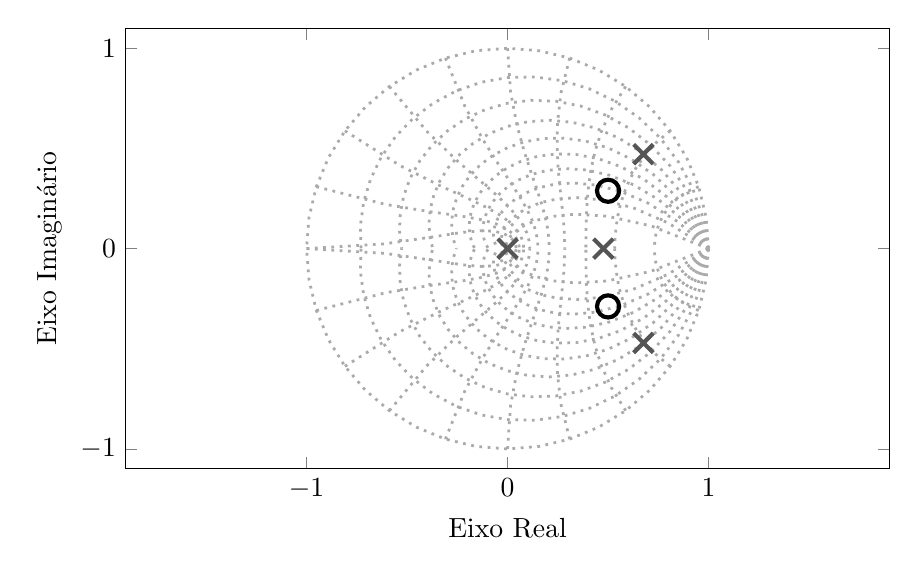
\begin{tikzpicture}

\begin{axis}[%
width=0.8\textwidth,
height=0.461611624834875\textwidth,
scale only axis,
xmin=-1.9,
xmax=1.9,
xtick={-1,  0,  1},
xlabel={Eixo Real},
ymin=-1.1,
ymax=1.1,
ytick={-1,  0,  1},
ylabel={Eixo Imaginário}
]
\addplot [color=mycolor1,dotted,line width=1.0pt,forget plot]
  table[row sep=crcr]{1	0\\
0.987688340595138	0.156434465040231\\
0.951056516295154	0.309016994374947\\
0.891006524188368	0.453990499739547\\
0.809016994374947	0.587785252292473\\
0.707106781186548	0.707106781186547\\
0.587785252292473	0.809016994374947\\
0.453990499739547	0.891006524188368\\
0.309016994374947	0.951056516295154\\
0.156434465040231	0.987688340595138\\
6.12323399573677e-17	1\\
-0.156434465040231	0.987688340595138\\
-0.309016994374947	0.951056516295154\\
-0.453990499739547	0.891006524188368\\
-0.587785252292473	0.809016994374947\\
-0.707106781186547	0.707106781186548\\
-0.809016994374947	0.587785252292473\\
-0.891006524188368	0.453990499739547\\
-0.951056516295154	0.309016994374948\\
-0.987688340595138	0.156434465040231\\
-1	1.22464679914735e-16\\
};
\addplot [color=mycolor1,dotted,line width=1.0pt,forget plot]
  table[row sep=crcr]{1	0\\
0.972218045703082	0.153984211042097\\
0.921496791140463	0.299412457456957\\
0.849791018366557	0.432990150609548\\
0.759508516401756	0.551815237548133\\
0.653437051516106	0.653437051516106\\
0.534664304371591	0.735902282058355\\
0.406492952796512	0.797787339572243\\
0.272353130096494	0.83821674479613\\
0.135714483753824	0.856867527364047\\
5.22899666167123e-17	0.853959960588124\\
-0.131496350792703	0.830235283991667\\
-0.255686250369537	0.786921363444393\\
-0.369756251949576	0.725687504552447\\
-0.47122811850853	0.648589862732789\\
-0.558009078759514	0.558009078759514\\
-0.628431083783263	0.456581908289041\\
-0.681278445058817	0.347128705949459\\
-0.715803538350409	0.232578668243255\\
-0.731730559897045	0.115894735197653\\
-0.729247614287671	8.9307075662324e-17\\
};
\addplot [color=mycolor1,dotted,line width=1.0pt,forget plot]
  table[row sep=crcr]{1	0\\
0.956521682769877	0.151498151383791\\
0.891982039736211	0.289822533396298\\
0.809292583610082	0.412355167436434\\
0.711634858347723	0.517032989000692\\
0.602364630186427	0.602364630186426\\
0.484917701774751	0.667431957639199\\
0.362719588349683	0.711877274647591\\
0.239101059900595	0.735877395777214\\
0.117221283062812	0.740106053489981\\
4.44354699422903e-17	0.725686295399261\\
-0.109940132237539	0.694134676438339\\
-0.210320240583588	0.647299141978847\\
-0.299240493845688	0.587292536894097\\
-0.375203754387119	0.516423664031337\\
-0.437127756959533	0.437127756959533\\
-0.484346224770267	0.351898130574443\\
-0.516599582217932	0.263220634338226\\
-0.534016141209622	0.173512362385299\\
-0.537084820159711	0.0850658786478001\\
-0.526620599330303	6.44924231334916e-17\\
};
\addplot [color=mycolor1,dotted,line width=1.0pt,forget plot]
  table[row sep=crcr]{1	0\\
0.940082788364644	0.148894486293864\\
0.86158608093073	0.279946287694513\\
0.768279786681378	0.391458103646313\\
0.663960650859636	0.482395649771645\\
0.552351927561387	0.552351927561387\\
0.437014383712816	0.601498696728173\\
0.321269860940431	0.630527604183869\\
0.208138182971344	0.640583459188477\\
0.100287778328637	0.633192112325829\\
3.73630739569174e-17	0.610185303761559\\
-0.0908532273476425	0.573624701779294\\
-0.170819110593797	0.525727164509449\\
-0.238861981883349	0.468793035010043\\
-0.294350736089166	0.40513903143051\\
-0.337037028702328	0.337037028702328\\
-0.367025664975262	0.266659754473976\\
-0.384738677688982	0.196034147687371\\
-0.390874612629551	0.127002860400749\\
-0.386364521398959	0.0611941284830315\\
-0.372326104926586	4.55967972637346e-17\\
};
\addplot [color=mycolor1,dotted,line width=1.0pt,forget plot]
  table[row sep=crcr]{1	0\\
0.922246029428501	0.146069421212559\\
0.829201462983264	0.269423887468404\\
0.725373165529273	0.369596088217499\\
0.614985835074999	0.446813363302878\\
0.501902475185001	0.501902475185001\\
0.38956496084428	0.536190168955128\\
0.280953750703967	0.551402782692681\\
0.178565395716864	0.549567778706978\\
0.0844061798404073	0.532919645815306\\
3.08495992433718e-17	0.50381218919366\\
-0.0735915548753502	0.464638791061534\\
-0.135739038566523	0.417761804348184\\
-0.186207014322272	0.365451842507638\\
-0.225110018726605	0.309837359892227\\
-0.252864584784672	0.252864584784672\\
-0.270139142845401	0.196267575756099\\
-0.277803443075876	0.141547924204336\\
-0.27687894570066	0.0899634229303457\\
-0.268491413422519	0.0425248622468694\\
-0.253826721980109	3.10848082611005e-17\\
};
\addplot [color=mycolor1,dotted,line width=1.0pt,forget plot]
  table[row sep=crcr]{1	0\\
0.902056570675584	0.142871725087523\\
0.793293726869509	0.257756756757911\\
0.678769666307395	0.345850419328459\\
0.562876391436159	0.408953636388562\\
0.449318435861499	0.449318435861499\\
0.341115747349381	0.469505547439701\\
0.24062663375655	0.472256359314945\\
0.149586755320764	0.460380694230177\\
0.069160331541479	0.436661148025441\\
2.47240337905553e-17	0.403774113610049\\
-0.057687904157153	0.364227092250654\\
-0.104075505986926	0.320311471399148\\
-0.139645446506012	0.274069620358657\\
-0.165124892040398	0.227274916024158\\
-0.18142315316863	0.18142315316863\\
-0.189574186252466	0.137733708524426\\
-0.190684892879101	0.0971588057560207\\
-0.185889806735969	0.0603992595374446\\
-0.176312467991919	0.0279251515651378\\
-0.16303353482158	1.99658496572927e-17\\
};
\addplot [color=mycolor1,dotted,line width=1.0pt,forget plot]
  table[row sep=crcr]{1	0\\
0.877921760602431	0.139049146701748\\
0.751411952540787	0.244148543365328\\
0.625732257688895	0.318826509862098\\
0.505011411193747	0.36691226736026\\
0.392341669548685	0.392341669548685\\
0.289890514921595	0.399000063654162\\
0.199020572856858	0.390599867100522\\
0.120411913496453	0.370589763847805\\
0.0541820486548744	0.34209199176291\\
1.88512313530119e-17	0.307863971328499\\
-0.042808222513439	0.270280479734772\\
-0.075164540154518	0.231332667812908\\
-0.0981551954909503	0.192640417840451\\
-0.112959067758674	0.155474818616317\\
-0.120787864504912	0.120787864504912\\
-0.122837744156894	0.0892468451742257\\
-0.120251626285951	0.0612712639357851\\
-0.114091236431876	0.0370704898842818\\
-0.105317799143806	0.0166807006736036\\
-0.0947802248421549	1.16072298975411e-17\\
};
\addplot [color=mycolor1,dotted,line width=1.0pt,forget plot]
  table[row sep=crcr]{1	0\\
0.84674396664984	0.134111069256013\\
0.698989566160914	0.227115477506975\\
0.561406498364893	0.286050898428465\\
0.437004973478602	0.317502698182059\\
0.327450698344114	0.327450698344114\\
0.233352139914598	0.321181666481713\\
0.154515499860225	0.303253743289057\\
0.0901653834921457	0.27750051639687\\
0.0391311034995635	0.247064063991275\\
1.31311479217367e-17	0.214447919692096\\
-0.0287598398096346	0.181582482159892\\
-0.0487044416812479	0.149896858349689\\
-0.0613430200940395	0.120392455675976\\
-0.06808779312177	0.0937148074575858\\
-0.0702211210616195	0.0702211210616195\\
-0.068876740220244	0.0500418809603846\\
-0.0650321343871793	0.0331355275052096\\
-0.0595094084547913	0.0193357789181307\\
-0.0529823745536039	0.00839158374073751\\
-0.0459879102602678	5.63189470997126e-18\\
};
\addplot [color=mycolor1,dotted,line width=1.0pt,forget plot]
  table[row sep=crcr]{1	0\\
0.801053465278425	0.126874404768154\\
0.625589539649299	0.203266363189334\\
0.475341369738971	0.242198525079547\\
0.350045057714404	0.254322621147605\\
0.24813777530853	0.24813777530853\\
0.167289292234614	0.230253957320141\\
0.104794333468008	0.205670459781722\\
0.0578515468028918	0.178048753195384\\
0.0237523524567972	0.149966451301199\\
7.54043881219821e-18	0.123144711070133\\
-0.0156239119173694	0.0986454975334405\\
-0.0250311775652273	0.0770380431086105\\
-0.0298254673925332	0.0585357756361869\\
-0.0313184856998208	0.0431061974937683\\
-0.0305568546459545	0.0305568546459545\\
-0.0283545570469435	0.0206007915573586\\
-0.0253272293454815	0.012904867916705\\
-0.021925762268643	0.00712411201600239\\
-0.0184675753156993	0.00292497658052826\\
-0.0151646198645466	1.85713031774033e-18\\
};
\addplot [color=mycolor1,dotted,line width=1.0pt,forget plot]
  table[row sep=crcr]{1	0\\
0.714110955679367	0.113104064044896\\
0.497161927717827	0.161537702532642\\
0.336758208677056	0.171586877647116\\
0.221075553032581	0.160620791180475\\
0.139705610200823	0.139705610200823\\
0.0839640345306934	0.115566579097864\\
0.0468885871776745	0.0920240337831981\\
0.0230753615892199	0.0710186604775083\\
0.00844586939409394	0.0533251206797082\\
2.39022368106624e-18	0.0390353150431684\\
-0.00441505277265522	0.0278755461307222\\
-0.00630567510971132	0.0194068724759343\\
-0.00669794782622876	0.0131454627690819\\
-0.0062698831862128	0.00862975386096949\\
-0.0054534525074872	0.0054534525074872\\
-0.00451117782354635	0.00327756254020109\\
-0.00359218715027031	0.00183031077240959\\
-0.00277223578568335	0.000900754009370227\\
-0.00208156288544739	0.000329687172611911\\
-0.00152375582051941	1.86606268828125e-19\\
};
\addplot [color=mycolor1,dotted,line width=1.0pt,forget plot]
  table[row sep=crcr]{1	-0\\
0.987688340595138	-0.156434465040231\\
0.951056516295154	-0.309016994374947\\
0.891006524188368	-0.453990499739547\\
0.809016994374947	-0.587785252292473\\
0.707106781186548	-0.707106781186547\\
0.587785252292473	-0.809016994374947\\
0.453990499739547	-0.891006524188368\\
0.309016994374947	-0.951056516295154\\
0.156434465040231	-0.987688340595138\\
6.12323399573677e-17	-1\\
-0.156434465040231	-0.987688340595138\\
-0.309016994374947	-0.951056516295154\\
-0.453990499739547	-0.891006524188368\\
-0.587785252292473	-0.809016994374947\\
-0.707106781186547	-0.707106781186548\\
-0.809016994374947	-0.587785252292473\\
-0.891006524188368	-0.453990499739547\\
-0.951056516295154	-0.309016994374948\\
-0.987688340595138	-0.156434465040231\\
-1	-1.22464679914735e-16\\
};
\addplot [color=mycolor1,dotted,line width=1.0pt,forget plot]
  table[row sep=crcr]{1	-0\\
0.972218045703082	-0.153984211042097\\
0.921496791140463	-0.299412457456957\\
0.849791018366557	-0.432990150609548\\
0.759508516401756	-0.551815237548133\\
0.653437051516106	-0.653437051516106\\
0.534664304371591	-0.735902282058355\\
0.406492952796512	-0.797787339572243\\
0.272353130096494	-0.83821674479613\\
0.135714483753824	-0.856867527364047\\
5.22899666167123e-17	-0.853959960588124\\
-0.131496350792703	-0.830235283991667\\
-0.255686250369537	-0.786921363444393\\
-0.369756251949576	-0.725687504552447\\
-0.47122811850853	-0.648589862732789\\
-0.558009078759514	-0.558009078759514\\
-0.628431083783263	-0.456581908289041\\
-0.681278445058817	-0.347128705949459\\
-0.715803538350409	-0.232578668243255\\
-0.731730559897045	-0.115894735197653\\
-0.729247614287671	-8.9307075662324e-17\\
};
\addplot [color=mycolor1,dotted,line width=1.0pt,forget plot]
  table[row sep=crcr]{1	-0\\
0.956521682769877	-0.151498151383791\\
0.891982039736211	-0.289822533396298\\
0.809292583610082	-0.412355167436434\\
0.711634858347723	-0.517032989000692\\
0.602364630186427	-0.602364630186426\\
0.484917701774751	-0.667431957639199\\
0.362719588349683	-0.711877274647591\\
0.239101059900595	-0.735877395777214\\
0.117221283062812	-0.740106053489981\\
4.44354699422903e-17	-0.725686295399261\\
-0.109940132237539	-0.694134676438339\\
-0.210320240583588	-0.647299141978847\\
-0.299240493845688	-0.587292536894097\\
-0.375203754387119	-0.516423664031337\\
-0.437127756959533	-0.437127756959533\\
-0.484346224770267	-0.351898130574443\\
-0.516599582217932	-0.263220634338226\\
-0.534016141209622	-0.173512362385299\\
-0.537084820159711	-0.0850658786478001\\
-0.526620599330303	-6.44924231334916e-17\\
};
\addplot [color=mycolor1,dotted,line width=1.0pt,forget plot]
  table[row sep=crcr]{1	-0\\
0.940082788364644	-0.148894486293864\\
0.86158608093073	-0.279946287694513\\
0.768279786681378	-0.391458103646313\\
0.663960650859636	-0.482395649771645\\
0.552351927561387	-0.552351927561387\\
0.437014383712816	-0.601498696728173\\
0.321269860940431	-0.630527604183869\\
0.208138182971344	-0.640583459188477\\
0.100287778328637	-0.633192112325829\\
3.73630739569174e-17	-0.610185303761559\\
-0.0908532273476425	-0.573624701779294\\
-0.170819110593797	-0.525727164509449\\
-0.238861981883349	-0.468793035010043\\
-0.294350736089166	-0.40513903143051\\
-0.337037028702328	-0.337037028702328\\
-0.367025664975262	-0.266659754473976\\
-0.384738677688982	-0.196034147687371\\
-0.390874612629551	-0.127002860400749\\
-0.386364521398959	-0.0611941284830315\\
-0.372326104926586	-4.55967972637346e-17\\
};
\addplot [color=mycolor1,dotted,line width=1.0pt,forget plot]
  table[row sep=crcr]{1	-0\\
0.922246029428501	-0.146069421212559\\
0.829201462983264	-0.269423887468404\\
0.725373165529273	-0.369596088217499\\
0.614985835074999	-0.446813363302878\\
0.501902475185001	-0.501902475185001\\
0.38956496084428	-0.536190168955128\\
0.280953750703967	-0.551402782692681\\
0.178565395716864	-0.549567778706978\\
0.0844061798404073	-0.532919645815306\\
3.08495992433718e-17	-0.50381218919366\\
-0.0735915548753502	-0.464638791061534\\
-0.135739038566523	-0.417761804348184\\
-0.186207014322272	-0.365451842507638\\
-0.225110018726605	-0.309837359892227\\
-0.252864584784672	-0.252864584784672\\
-0.270139142845401	-0.196267575756099\\
-0.277803443075876	-0.141547924204336\\
-0.27687894570066	-0.0899634229303457\\
-0.268491413422519	-0.0425248622468694\\
-0.253826721980109	-3.10848082611005e-17\\
};
\addplot [color=mycolor1,dotted,line width=1.0pt,forget plot]
  table[row sep=crcr]{1	-0\\
0.902056570675584	-0.142871725087523\\
0.793293726869509	-0.257756756757911\\
0.678769666307395	-0.345850419328459\\
0.562876391436159	-0.408953636388562\\
0.449318435861499	-0.449318435861499\\
0.341115747349381	-0.469505547439701\\
0.24062663375655	-0.472256359314945\\
0.149586755320764	-0.460380694230177\\
0.069160331541479	-0.436661148025441\\
2.47240337905553e-17	-0.403774113610049\\
-0.057687904157153	-0.364227092250654\\
-0.104075505986926	-0.320311471399148\\
-0.139645446506012	-0.274069620358657\\
-0.165124892040398	-0.227274916024158\\
-0.18142315316863	-0.18142315316863\\
-0.189574186252466	-0.137733708524426\\
-0.190684892879101	-0.0971588057560207\\
-0.185889806735969	-0.0603992595374446\\
-0.176312467991919	-0.0279251515651378\\
-0.16303353482158	-1.99658496572927e-17\\
};
\addplot [color=mycolor1,dotted,line width=1.0pt,forget plot]
  table[row sep=crcr]{1	-0\\
0.877921760602431	-0.139049146701748\\
0.751411952540787	-0.244148543365328\\
0.625732257688895	-0.318826509862098\\
0.505011411193747	-0.36691226736026\\
0.392341669548685	-0.392341669548685\\
0.289890514921595	-0.399000063654162\\
0.199020572856858	-0.390599867100522\\
0.120411913496453	-0.370589763847805\\
0.0541820486548744	-0.34209199176291\\
1.88512313530119e-17	-0.307863971328499\\
-0.042808222513439	-0.270280479734772\\
-0.075164540154518	-0.231332667812908\\
-0.0981551954909503	-0.192640417840451\\
-0.112959067758674	-0.155474818616317\\
-0.120787864504912	-0.120787864504912\\
-0.122837744156894	-0.0892468451742257\\
-0.120251626285951	-0.0612712639357851\\
-0.114091236431876	-0.0370704898842818\\
-0.105317799143806	-0.0166807006736036\\
-0.0947802248421549	-1.16072298975411e-17\\
};
\addplot [color=mycolor1,dotted,line width=1.0pt,forget plot]
  table[row sep=crcr]{1	-0\\
0.84674396664984	-0.134111069256013\\
0.698989566160914	-0.227115477506975\\
0.561406498364893	-0.286050898428465\\
0.437004973478602	-0.317502698182059\\
0.327450698344114	-0.327450698344114\\
0.233352139914598	-0.321181666481713\\
0.154515499860225	-0.303253743289057\\
0.0901653834921457	-0.27750051639687\\
0.0391311034995635	-0.247064063991275\\
1.31311479217367e-17	-0.214447919692096\\
-0.0287598398096346	-0.181582482159892\\
-0.0487044416812479	-0.149896858349689\\
-0.0613430200940395	-0.120392455675976\\
-0.06808779312177	-0.0937148074575858\\
-0.0702211210616195	-0.0702211210616195\\
-0.068876740220244	-0.0500418809603846\\
-0.0650321343871793	-0.0331355275052096\\
-0.0595094084547913	-0.0193357789181307\\
-0.0529823745536039	-0.00839158374073751\\
-0.0459879102602678	-5.63189470997126e-18\\
};
\addplot [color=mycolor1,dotted,line width=1.0pt,forget plot]
  table[row sep=crcr]{1	-0\\
0.801053465278425	-0.126874404768154\\
0.625589539649299	-0.203266363189334\\
0.475341369738971	-0.242198525079547\\
0.350045057714404	-0.254322621147605\\
0.24813777530853	-0.24813777530853\\
0.167289292234614	-0.230253957320141\\
0.104794333468008	-0.205670459781722\\
0.0578515468028918	-0.178048753195384\\
0.0237523524567972	-0.149966451301199\\
7.54043881219821e-18	-0.123144711070133\\
-0.0156239119173694	-0.0986454975334405\\
-0.0250311775652273	-0.0770380431086105\\
-0.0298254673925332	-0.0585357756361869\\
-0.0313184856998208	-0.0431061974937683\\
-0.0305568546459545	-0.0305568546459545\\
-0.0283545570469435	-0.0206007915573586\\
-0.0253272293454815	-0.012904867916705\\
-0.021925762268643	-0.00712411201600239\\
-0.0184675753156993	-0.00292497658052826\\
-0.0151646198645466	-1.85713031774033e-18\\
};
\addplot [color=mycolor1,dotted,line width=1.0pt,forget plot]
  table[row sep=crcr]{1	-0\\
0.714110955679367	-0.113104064044896\\
0.497161927717827	-0.161537702532642\\
0.336758208677056	-0.171586877647116\\
0.221075553032581	-0.160620791180475\\
0.139705610200823	-0.139705610200823\\
0.0839640345306934	-0.115566579097864\\
0.0468885871776745	-0.0920240337831981\\
0.0230753615892199	-0.0710186604775083\\
0.00844586939409394	-0.0533251206797082\\
2.39022368106624e-18	-0.0390353150431684\\
-0.00441505277265522	-0.0278755461307222\\
-0.00630567510971132	-0.0194068724759343\\
-0.00669794782622876	-0.0131454627690819\\
-0.0062698831862128	-0.00862975386096949\\
-0.0054534525074872	-0.0054534525074872\\
-0.00451117782354635	-0.00327756254020109\\
-0.00359218715027031	-0.00183031077240959\\
-0.00277223578568335	-0.000900754009370227\\
-0.00208156288544739	-0.000329687172611911\\
-0.00152375582051941	-1.86606268828125e-19\\
};
\addplot [color=mycolor1,dotted,line width=1.0pt,forget plot]
  table[row sep=crcr]{1	0\\
1	0\\
};
\addplot [color=mycolor1,dotted,line width=1.0pt,forget plot]
  table[row sep=crcr]{0.951056516295154	0.309016994374947\\
0.906577591518048	0.290693092532446\\
0.867277205719189	0.267124444629623\\
0.833330533437629	0.239553777474139\\
0.804679893747523	0.20903820245934\\
0.781122098933164	0.176433510213537\\
0.762382187756933	0.142402376999381\\
0.748171074803624	0.107437628337747\\
0.738227708485823	0.0718935522249012\\
0.732347931289196	0.0360204899377399\\
0.730402691048646	2.81010850277162e-17\\
};
\addplot [color=mycolor1,dotted,line width=1.0pt,forget plot]
  table[row sep=crcr]{0.809016994374947	0.587785252292473\\
0.737380455396588	0.527071687397996\\
0.6808142826414	0.463341883835339\\
0.637053765657314	0.399254954339046\\
0.603812761314093	0.336417677088311\\
0.579022949915482	0.275632227640288\\
0.560948163233974	0.217130071437151\\
0.54821711318997	0.160763451735608\\
0.539811466724715	0.106147624627789\\
0.535036016768209	0.0527590625798542\\
0.533488091091103	4.10502162512614e-17\\
};
\addplot [color=mycolor1,dotted,line width=1.0pt,forget plot]
  table[row sep=crcr]{0.587785252292473	0.809016994374947\\
0.515276498489902	0.692182785870847\\
0.46668476526979	0.583707991451876\\
0.435233321876477	0.485319980094308\\
0.415551842123536	0.396928474901319\\
0.403656860517901	0.317461475735791\\
0.396737049613855	0.245416450708029\\
0.392888142823216	0.179177710929467\\
0.39087245229983	0.11717008156476\\
0.389932112762627	0.0579102497954412\\
0.389661137375347	4.49747826270753e-17\\
};
\addplot [color=mycolor1,dotted,line width=1.0pt,forget plot]
  table[row sep=crcr]{0.309016994374947	0.951056516295154\\
0.265925372344309	0.777304721760365\\
0.248822386132444	0.630899544522142\\
0.24643298177389	0.508693744238057\\
0.251412997268255	0.406266573115132\\
0.25929445161488	0.31919477108011\\
0.267517373913267	0.243597429511063\\
0.274697115780397	0.1762665508339\\
0.280129101393366	0.114599409879343\\
0.283480020554887	0.0564559973822998\\
0.284609543336029	4.37996030135249e-17\\
};
\addplot [color=mycolor1,dotted,line width=1.0pt,forget plot]
  table[row sep=crcr]{6.12323399573677e-17	1\\
0.0151248701748503	0.781989711398728\\
0.0472692933177679	0.613631335769719\\
0.0835006201485716	0.482943980920436\\
0.117381749765263	0.379469463911326\\
0.146223972383669	0.295078319831894\\
0.169261627793672	0.223809451176491\\
0.186582776182006	0.161390341419992\\
0.198560105942714	0.104739935929793\\
0.205572433929556	0.0515565221197431\\
0.207879576350762	3.99891848849262e-17\\
};
\addplot [color=mycolor1,dotted,line width=1.0pt,forget plot]
  table[row sep=crcr]{-0.309016994374947	0.951056516295154\\
-0.213607139159912	0.713331044437031\\
-0.122920349149865	0.544815253953639\\
-0.0461074386071066	0.422454854218942\\
0.0151311193047769	0.329888717873058\\
0.0621570724668225	0.256291005261778\\
0.0971710522581798	0.194731597161215\\
0.122256440677152	0.140793596164787\\
0.13905244595299	0.0915971142347777\\
0.148693455532156	0.0451621321066958\\
0.151835801980649	3.50498499033503e-17\\
};
\addplot [color=mycolor1,dotted,line width=1.0pt,forget plot]
  table[row sep=crcr]{-0.587785252292473	0.809016994374948\\
-0.401011853057454	0.584595820351374\\
-0.252139489074835	0.439670821081765\\
-0.139623392550337	0.340999317931598\\
-0.0567836371213516	0.268617800427267\\
0.0033339412143336	0.21116115844769\\
0.0463512370945915	0.162297289886265\\
0.0763422025660035	0.118472638203443\\
0.0960671266193367	0.0776165020305757\\
0.1072685824301	0.0384304051397518\\
0.110901278364195	2.98672554719679e-17\\
};
\addplot [color=mycolor1,dotted,line width=1.0pt,forget plot]
  table[row sep=crcr]{-0.809016994374948	0.587785252292473\\
-0.533486326814499	0.413410095118228\\
-0.336121655437603	0.313963860155743\\
-0.198040110920963	0.250717832404618\\
-0.101844033235305	0.204281393673556\\
-0.0346516892466227	0.165530866251108\\
0.0122258376810533	0.130333089269644\\
0.0443886084751889	0.0968398262452624\\
0.065339288702761	0.0642052594194206\\
0.0771736424133687	0.032008294596762\\
0.0810025921579431	2.49315700239574e-17\\
};
\addplot [color=mycolor1,dotted,line width=1.0pt,forget plot]
  table[row sep=crcr]{-0.951056516295154	0.309016994374948\\
-0.60382220830535	0.219707538176049\\
-0.375378071887508	0.182507388795924\\
-0.225093275108467	0.161489568357552\\
-0.124654461172013	0.143091836517116\\
-0.0562723920172722	0.12318609851568\\
-0.00923898083522721	0.101104614081101\\
0.0228060316514889	0.0772217637055013\\
0.0436193292019494	0.0520955750986265\\
0.0553650029180358	0.0262210407420432\\
0.0591645112940776	2.0486346567262e-17\\
};
\addplot [color=mycolor1,dotted,line width=1.0pt,forget plot]
  table[row sep=crcr]{-1	1.22464679914735e-16\\
-0.61127914703566	0.0236549857259488\\
-0.374309030147768	0.0580118391989452\\
-0.226262535142082	0.0806522438077526\\
-0.130218598863194	0.0890855793127953\\
-0.0656897647351535	0.0862950481802363\\
-0.0214411717925588	0.0757647040434823\\
0.00876629006412298	0.0602253159022079\\
0.0284556614934045	0.0415943455493057\\
0.039601950618638	0.0211971994741971\\
0.0432139182637723	1.66258696249815e-17\\
};
\addplot [color=mycolor1,dotted,line width=1.0pt,forget plot]
  table[row sep=crcr]{1	-0\\
1	-0\\
};
\addplot [color=mycolor1,dotted,line width=1.0pt,forget plot]
  table[row sep=crcr]{0.951056516295154	-0.309016994374947\\
0.906577591518048	-0.290693092532446\\
0.867277205719189	-0.267124444629623\\
0.833330533437629	-0.239553777474139\\
0.804679893747523	-0.20903820245934\\
0.781122098933164	-0.176433510213537\\
0.762382187756933	-0.142402376999381\\
0.748171074803624	-0.107437628337747\\
0.738227708485823	-0.0718935522249012\\
0.732347931289196	-0.0360204899377399\\
0.730402691048646	-2.81010850277162e-17\\
};
\addplot [color=mycolor1,dotted,line width=1.0pt,forget plot]
  table[row sep=crcr]{0.809016994374947	-0.587785252292473\\
0.737380455396588	-0.527071687397996\\
0.6808142826414	-0.463341883835339\\
0.637053765657314	-0.399254954339046\\
0.603812761314093	-0.336417677088311\\
0.579022949915482	-0.275632227640288\\
0.560948163233974	-0.217130071437151\\
0.54821711318997	-0.160763451735608\\
0.539811466724715	-0.106147624627789\\
0.535036016768209	-0.0527590625798542\\
0.533488091091103	-4.10502162512614e-17\\
};
\addplot [color=mycolor1,dotted,line width=1.0pt,forget plot]
  table[row sep=crcr]{0.587785252292473	-0.809016994374947\\
0.515276498489902	-0.692182785870847\\
0.46668476526979	-0.583707991451876\\
0.435233321876477	-0.485319980094308\\
0.415551842123536	-0.396928474901319\\
0.403656860517901	-0.317461475735791\\
0.396737049613855	-0.245416450708029\\
0.392888142823216	-0.179177710929467\\
0.39087245229983	-0.11717008156476\\
0.389932112762627	-0.0579102497954412\\
0.389661137375347	-4.49747826270753e-17\\
};
\addplot [color=mycolor1,dotted,line width=1.0pt,forget plot]
  table[row sep=crcr]{0.309016994374947	-0.951056516295154\\
0.265925372344309	-0.777304721760365\\
0.248822386132444	-0.630899544522142\\
0.24643298177389	-0.508693744238057\\
0.251412997268255	-0.406266573115132\\
0.25929445161488	-0.31919477108011\\
0.267517373913267	-0.243597429511063\\
0.274697115780397	-0.1762665508339\\
0.280129101393366	-0.114599409879343\\
0.283480020554887	-0.0564559973822998\\
0.284609543336029	-4.37996030135249e-17\\
};
\addplot [color=mycolor1,dotted,line width=1.0pt,forget plot]
  table[row sep=crcr]{6.12323399573677e-17	-1\\
0.0151248701748503	-0.781989711398728\\
0.0472692933177679	-0.613631335769719\\
0.0835006201485716	-0.482943980920436\\
0.117381749765263	-0.379469463911326\\
0.146223972383669	-0.295078319831894\\
0.169261627793672	-0.223809451176491\\
0.186582776182006	-0.161390341419992\\
0.198560105942714	-0.104739935929793\\
0.205572433929556	-0.0515565221197431\\
0.207879576350762	-3.99891848849262e-17\\
};
\addplot [color=mycolor1,dotted,line width=1.0pt,forget plot]
  table[row sep=crcr]{-0.309016994374947	-0.951056516295154\\
-0.213607139159912	-0.713331044437031\\
-0.122920349149865	-0.544815253953639\\
-0.0461074386071066	-0.422454854218942\\
0.0151311193047769	-0.329888717873058\\
0.0621570724668225	-0.256291005261778\\
0.0971710522581798	-0.194731597161215\\
0.122256440677152	-0.140793596164787\\
0.13905244595299	-0.0915971142347777\\
0.148693455532156	-0.0451621321066958\\
0.151835801980649	-3.50498499033503e-17\\
};
\addplot [color=mycolor1,dotted,line width=1.0pt,forget plot]
  table[row sep=crcr]{-0.587785252292473	-0.809016994374948\\
-0.401011853057454	-0.584595820351374\\
-0.252139489074835	-0.439670821081765\\
-0.139623392550337	-0.340999317931598\\
-0.0567836371213516	-0.268617800427267\\
0.0033339412143336	-0.21116115844769\\
0.0463512370945915	-0.162297289886265\\
0.0763422025660035	-0.118472638203443\\
0.0960671266193367	-0.0776165020305757\\
0.1072685824301	-0.0384304051397518\\
0.110901278364195	-2.98672554719679e-17\\
};
\addplot [color=mycolor1,dotted,line width=1.0pt,forget plot]
  table[row sep=crcr]{-0.809016994374948	-0.587785252292473\\
-0.533486326814499	-0.413410095118228\\
-0.336121655437603	-0.313963860155743\\
-0.198040110920963	-0.250717832404618\\
-0.101844033235305	-0.204281393673556\\
-0.0346516892466227	-0.165530866251108\\
0.0122258376810533	-0.130333089269644\\
0.0443886084751889	-0.0968398262452624\\
0.065339288702761	-0.0642052594194206\\
0.0771736424133687	-0.032008294596762\\
0.0810025921579431	-2.49315700239574e-17\\
};
\addplot [color=mycolor1,dotted,line width=1.0pt,forget plot]
  table[row sep=crcr]{-0.951056516295154	-0.309016994374948\\
-0.60382220830535	-0.219707538176049\\
-0.375378071887508	-0.182507388795924\\
-0.225093275108467	-0.161489568357552\\
-0.124654461172013	-0.143091836517116\\
-0.0562723920172722	-0.12318609851568\\
-0.00923898083522721	-0.101104614081101\\
0.0228060316514889	-0.0772217637055013\\
0.0436193292019494	-0.0520955750986265\\
0.0553650029180358	-0.0262210407420432\\
0.0591645112940776	-2.0486346567262e-17\\
};
\addplot [color=mycolor1,dotted,line width=1.0pt,forget plot]
  table[row sep=crcr]{-1	-1.22464679914735e-16\\
-0.61127914703566	-0.0236549857259488\\
-0.374309030147768	-0.0580118391989452\\
-0.226262535142082	-0.0806522438077526\\
-0.130218598863194	-0.0890855793127953\\
-0.0656897647351535	-0.0862950481802363\\
-0.0214411717925588	-0.0757647040434823\\
0.00876629006412298	-0.0602253159022079\\
0.0284556614934045	-0.0415943455493057\\
0.039601950618638	-0.0211971994741971\\
0.0432139182637723	-1.66258696249815e-17\\
};
\addplot [color=black!50!mycolor1,line width=1.5pt,mark size=5.0pt,only marks,mark=x,mark options={solid},forget plot]
  table[row sep=crcr]{0	0\\
0.676084684146394	0.471252951045488\\
0.676084684146394	-0.471252951045488\\
0.476716764894897	0\\
};
\addplot [color=black,line width=1.5pt,mark size=4.0pt,only marks,mark=o,mark options={solid},forget plot]
  table[row sep=crcr]{0.500166366019944	0.288659057024714\\
0.500166366019944	-0.288659057024714\\
};
\end{axis}
\end{tikzpicture}%}
    \captionof{figure}{Diagrama de pólos e zeros para $\Delta(z)$ considerando $i_C$ como variável intermediária.}
    \label{fig:pzmap_delta_ic}
  \end{minipage}
  \vspace{\fill}

  \newpage

  \vspace*{\fill}
  \noindent
  \begin{minipage}{\textwidth}
    \makebox[\textwidth]{
      \centering
      \def\svgwidth{\textwidth}
      % This file was created by matlab2tikz v0.4.7 running on MATLAB 7.14.
% Copyright (c) 2008--2014, Nico Schlömer <nico.schloemer@gmail.com>
% All rights reserved.
% Minimal pgfplots version: 1.3
% 
% The latest updates can be retrieved from
%   http://www.mathworks.com/matlabcentral/fileexchange/22022-matlab2tikz
% where you can also make suggestions and rate matlab2tikz.
% 
%
% defining custom colors
\definecolor{mycolor1}{rgb}{0.66667,0.66667,0.66667}%
%
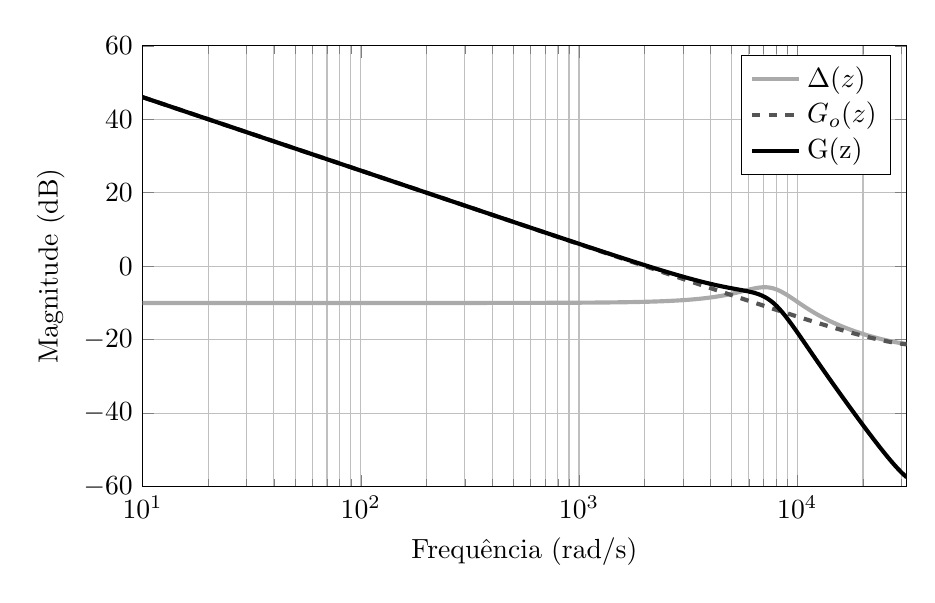
\begin{tikzpicture}

\begin{axis}[%
width=0.8\textwidth,
height=0.461611624834875\textwidth,
scale only axis,
xmode=log,
xmin=10,
xmax=31622.7766016838,
xminorticks=true,
xlabel={Frequência (rad/s)},
xmajorgrids,
xminorgrids,
ymin=-60,
ymax=60,
ylabel={Magnitude (dB)},
ymajorgrids,
legend style={draw=black,fill=white,legend cell align=left}
]
\addplot [color=mycolor1,solid,line width=1.5pt]
  table[row sep=crcr]{10	-10.0200805450291\\
10.0461810465159	-10.020080477148\\
10.0925753619375	-10.0200804086386\\
10.139183931163	-10.0200803394949\\
10.1860077436388	-10.0200802697111\\
10.2330477933808	-10.0200801992812\\
10.2803050789954	-10.0200801281994\\
10.3277806037004	-10.0200800564595\\
10.375475375347	-10.0200799840555\\
10.4233904064403	-10.0200799109812\\
10.4715267141616	-10.0200798372304\\
10.5198853203895	-10.0200797627968\\
10.5684672517218	-10.0200796876742\\
10.6172735394972	-10.0200796118561\\
10.6663052198171	-10.0200795353361\\
10.715563333568	-10.0200794581078\\
10.7650489264432	-10.0200793801645\\
10.814763048965	-10.0200793014996\\
10.8647067565072	-10.0200792221065\\
10.9148811093176	-10.0200791419783\\
10.9652871725401	-10.0200790611084\\
11.0159260162376	-10.0200789794899\\
11.0667987154147	-10.0200788971157\\
11.1179063500406	-10.020078813979\\
11.1692500050717	-10.0200787300726\\
11.2208307704748	-10.0200786453894\\
11.2726497412507	-10.0200785599223\\
11.3247080174565	-10.020078473664\\
11.3770067042298	-10.0200783866071\\
11.4295469118117	-10.0200782987443\\
11.4823297555707	-10.0200782100681\\
11.535356356026	-10.020078120571\\
11.5886278388715	-10.0200780302453\\
11.6421453349997	-10.0200779390834\\
11.6959099805258	-10.0200778470776\\
11.7499229168114	-10.0200777542201\\
11.8041852904894	-10.0200776605029\\
11.8586982534876	-10.0200775659181\\
11.9134629630538	-10.0200774704577\\
11.96848058178	-10.0200773741135\\
12.0237522776272	-10.0200772768775\\
12.0792792239501	-10.0200771787413\\
12.135062599522	-10.0200770796965\\
12.1911035885602	-10.0200769797349\\
12.2474033807505	-10.0200768788478\\
12.3039631712731	-10.0200767770268\\
12.3607841608273	-10.0200766742632\\
12.4178675556577	-10.0200765705482\\
12.4752145675793	-10.020076465873\\
12.5328264140034	-10.0200763602288\\
12.5907043179635	-10.0200762536067\\
12.6488495081411	-10.0200761459974\\
12.7072632188919	-10.020076037392\\
12.765946690272	-10.0200759277811\\
12.8249011680643	-10.0200758171555\\
12.8841279038047	-10.0200757055057\\
12.9436281548089	-10.0200755928224\\
13.0034031841991	-10.0200754790959\\
13.0634542609305	-10.0200753643165\\
13.1237826598188	-10.0200752484746\\
13.1843896615665	-10.0200751315602\\
13.2452765527909	-10.0200750135635\\
13.306444626051	-10.0200748944744\\
13.3678951798747	-10.0200747742829\\
13.4296295187868	-10.0200746529786\\
13.4916489533366	-10.0200745305514\\
13.5539548001256	-10.0200744069908\\
13.6165483818355	-10.0200742822863\\
13.6794310272563	-10.0200741564274\\
13.7426040713143	-10.0200740294033\\
13.806068855101	-10.0200739012033\\
13.8698267259009	-10.0200737718164\\
13.9338790372205	-10.0200736412318\\
13.998227148817	-10.0200735094382\\
14.062872426727	-10.0200733764245\\
14.1278162432955	-10.0200732421795\\
14.1930599772055	-10.0200731066916\\
14.2586050135065	-10.0200729699495\\
14.3244527436445	-10.0200728319414\\
14.3906045654914	-10.0200726926558\\
14.4570618833745	-10.0200725520807\\
14.5238261081064	-10.0200724102042\\
14.5908986570152	-10.0200722670142\\
14.658280953974	-10.0200721224987\\
14.7259744294318	-10.0200719766453\\
14.7939805204436	-10.0200718294416\\
14.8623006707006	-10.0200716808752\\
14.9309363305612	-10.0200715309334\\
14.999888957082	-10.0200713796035\\
15.069160014048	-10.0200712268727\\
15.1387509720044	-10.0200710727279\\
15.2086633082875	-10.0200709171561\\
15.2788985070559	-10.0200707601441\\
15.3494580593225	-10.0200706016786\\
15.4203434629857	-10.020070441746\\
15.4915562228612	-10.0200702803328\\
15.5630978507143	-10.0200701174253\\
15.6349698652918	-10.0200699530097\\
15.7071737923542	-10.020069787072\\
15.779711164708	-10.0200696195981\\
15.8525835222385	-10.0200694505738\\
15.9257924119422	-10.0200692799847\\
15.9993393879601	-10.0200691078164\\
16.07322601161	-10.0200689340542\\
16.1474538514202	-10.0200687586834\\
16.2220244831628	-10.0200685816891\\
16.2969394898867	-10.0200684030562\\
16.3722004619516	-10.0200682227696\\
16.4478089970617	-10.020068040814\\
16.5237667002994	-10.0200678571739\\
16.6000751841599	-10.0200676718337\\
16.6767360685846	-10.0200674847777\\
16.7537509809962	-10.02006729599\\
16.8311215563331	-10.0200671054546\\
16.9088494370839	-10.0200669131553\\
16.9869362733223	-10.0200667190757\\
17.0653837227424	-10.0200665231994\\
17.1441934506935	-10.0200663255098\\
17.2233671302159	-10.02006612599\\
17.302906442076	-10.0200659246232\\
17.3828130748022	-10.0200657213922\\
17.4630887247206	-10.0200655162797\\
17.5437350959914	-10.0200653092684\\
17.6247539006444	-10.0200651003406\\
17.7061468586161	-10.0200648894786\\
17.7879156977856	-10.0200646766646\\
17.8700621540116	-10.0200644618804\\
17.9525879711692	-10.0200642451078\\
18.035494901187	-10.0200640263284\\
18.1187847040838	-10.0200638055237\\
18.2024591480069	-10.0200635826747\\
18.2865200092687	-10.0200633577628\\
18.3709690723849	-10.0200631307687\\
18.4558081301122	-10.0200629016731\\
18.5410389834868	-10.0200626704567\\
18.6266634418617	-10.0200624370997\\
18.7126833229461	-10.0200622015824\\
18.7991004528435	-10.0200619638847\\
18.8859166660905	-10.0200617239866\\
18.9731338056957	-10.0200614818675\\
19.060753723179	-10.020061237507\\
19.1487782786108	-10.0200609908842\\
19.2372093406515	-10.0200607419783\\
19.3260487865912	-10.0200604907682\\
19.4152985023894	-10.0200602372324\\
19.5049603827153	-10.0200599813494\\
19.5950363309877	-10.0200597230976\\
19.6855282594159	-10.020059462455\\
19.7764380890397	-10.0200591993994\\
19.8677677497706	-10.0200589339085\\
19.9595191804325	-10.0200586659598\\
20.0516943288031	-10.0200583955306\\
20.1442951516552	-10.0200581225978\\
20.2373236147981	-10.0200578471382\\
20.3307816931193	-10.0200575691286\\
20.4246713706267	-10.0200572885452\\
20.5189946404906	-10.0200570053642\\
20.6137535050858	-10.0200567195617\\
20.7089499760343	-10.0200564311133\\
20.8045860742482	-10.0200561399945\\
20.900663829972	-10.0200558461806\\
20.9971852828265	-10.0200555496467\\
21.0941524818514	-10.0200552503676\\
21.1915674855492	-10.0200549483179\\
21.2894323619287	-10.0200546434718\\
21.387749188549	-10.0200543358036\\
21.4865200525637	-10.0200540252871\\
21.5857470507649	-10.0200537118959\\
21.685432289628	-10.0200533956035\\
21.7855778853565	-10.0200530763829\\
21.8861859639264	-10.020052754207\\
21.987258661132	-10.0200524290486\\
22.0887981226306	-10.0200521008799\\
22.1908065039887	-10.0200517696731\\
22.2932859707273	-10.0200514354001\\
22.396238698368	-10.0200510980325\\
22.499666872479	-10.0200507575417\\
22.603572688722	-10.0200504138987\\
22.7079583528983	-10.0200500670743\\
22.8128260809959	-10.0200497170391\\
22.9181780992365	-10.0200493637634\\
23.0240166441225	-10.0200490072172\\
23.130343962485	-10.0200486473702\\
23.237162311531	-10.0200482841918\\
23.3444739588916	-10.0200479176512\\
23.4522811826701	-10.0200475477173\\
23.5605862714901	-10.0200471743586\\
23.6693915245447	-10.0200467975434\\
23.7786992516445	-10.0200464172398\\
23.8885117732672	-10.0200460334155\\
23.9988314206069	-10.0200456460378\\
24.1096605356231	-10.0200452550739\\
24.2210014710909	-10.0200448604905\\
24.3328565906507	-10.0200444622542\\
24.4452282688584	-10.0200440603311\\
24.558118891236	-10.0200436546871\\
24.6715308543219	-10.0200432452877\\
24.7854665657221	-10.0200428320983\\
24.899928444161	-10.0200424150836\\
25.0149189195332	-10.0200419942083\\
25.1304404329547	-10.0200415694366\\
25.2464954368146	-10.0200411407326\\
25.3630863948276	-10.0200407080596\\
25.4802157820863	-10.0200402713811\\
25.597886085113	-10.0200398306599\\
25.7160998019135	-10.0200393858587\\
25.8348594420295	-10.0200389369395\\
25.9541675265918	-10.0200384838644\\
26.0740265883745	-10.0200380265948\\
26.194439171848	-10.0200375650919\\
26.3154078332332	-10.0200370993165\\
26.4369351405564	-10.020036629229\\
26.5590236737027	-10.0200361547896\\
26.6816760244719	-10.020035675958\\
26.8048947966327	-10.0200351926934\\
26.9286826059784	-10.0200347049548\\
27.0530420803822	-10.0200342127009\\
27.1779758598533	-10.0200337158897\\
27.3034865965925	-10.0200332144793\\
27.4295769550488	-10.0200327084268\\
27.556249611976	-10.0200321976894\\
27.6835072564894	-10.0200316822237\\
27.8113525901229	-10.0200311619859\\
27.9397883268864	-10.0200306369319\\
28.0688171933232	-10.020030107017\\
28.1984419285683	-10.0200295721962\\
28.3286652844062	-10.0200290324242\\
28.4594900253294	-10.0200284876551\\
28.5909189285972	-10.0200279378426\\
28.7229547842946	-10.02002738294\\
28.8556003953913	-10.0200268229002\\
28.9888585778017	-10.0200262576757\\
29.1227321604441	-10.0200256872184\\
29.2572239853012	-10.0200251114799\\
29.3923369074803	-10.0200245304113\\
29.5280737952738	-10.0200239439633\\
29.6644375302202	-10.0200233520861\\
29.8014310071653	-10.0200227547293\\
29.9390571343235	-10.0200221518423\\
30.0773188333397	-10.0200215433738\\
30.2162190393513	-10.0200209292722\\
30.3557607010504	-10.0200203094854\\
30.4959467807464	-10.0200196839607\\
30.6367802544292	-10.0200190526449\\
30.7782641118319	-10.0200184154845\\
30.9204013564946	-10.0200177724254\\
31.063195005828	-10.0200171234129\\
31.2066480911777	-10.0200164683919\\
31.350763657888	-10.0200158073068\\
31.4955447653674	-10.0200151401014\\
31.6409944871527	-10.0200144667192\\
31.7871159109747	-10.0200137871028\\
31.9339121388238	-10.0200131011947\\
32.0813862870155	-10.0200124089364\\
32.229541486257	-10.0200117102693\\
32.3783808817133	-10.020011005134\\
32.5279076330741	-10.0200102934707\\
32.6781249146208	-10.0200095752188\\
32.8290359152942	-10.0200088503174\\
32.9806438387618	-10.0200081187049\\
33.132951903486	-10.0200073803192\\
33.2859633427924	-10.0200066350976\\
33.4396814049384	-10.0200058829768\\
33.5941093531822	-10.0200051238929\\
33.7492504658521	-10.0200043577815\\
33.9051080364161	-10.0200035845774\\
34.0616853735517	-10.0200028042151\\
34.2189858012163	-10.0200020166282\\
34.3770126587175	-10.0200012217498\\
34.5357693007845	-10.0200004195125\\
34.6952590976386	-10.0199996098482\\
34.8554854350656	-10.019998792688\\
35.0164517144866	-10.0199979679625\\
35.1781613530314	-10.0199971356018\\
35.3406177836102	-10.0199962955351\\
35.5038244549868	-10.0199954476911\\
35.6677848318515	-10.0199945919977\\
35.8325023948954	-10.0199937283824\\
35.9979806408833	-10.0199928567717\\
36.1642230827288	-10.0199919770916\\
36.3312332495683	-10.0199910892675\\
36.4990146868361	-10.0199901932238\\
36.6675709563398	-10.0199892888846\\
36.8369056363357	-10.0199883761731\\
37.007022321605	-10.0199874550116\\
37.1779246235299	-10.019986525322\\
37.3496161701703	-10.0199855870253\\
37.5221006063408	-10.0199846400418\\
37.6953815936883	-10.0199836842911\\
37.8694628107696	-10.019982719692\\
38.0443479531292	-10.0199817461627\\
38.2200407333782	-10.0199807636203\\
38.3965448812729	-10.0199797719815\\
38.5738641437941	-10.0199787711621\\
38.7520022852263	-10.019977761077\\
38.9309630872381	-10.0199767416405\\
39.1107503489621	-10.019975712766\\
39.2913678870758	-10.019974674366\\
39.4728195358824	-10.0199736263525\\
39.6551091473924	-10.0199725686364\\
39.8382405914052	-10.0199715011278\\
40.0222177555915	-10.0199704237361\\
40.2070445455755	-10.0199693363698\\
40.3927248850181	-10.0199682389366\\
40.5792627157	-10.0199671313432\\
40.7666619976054	-10.0199660134956\\
40.9549267090063	-10.0199648852988\\
41.1440608465467	-10.019963746657\\
41.3340684253274	-10.0199625974735\\
41.5249534789915	-10.0199614376508\\
41.7167200598098	-10.0199602670902\\
41.9093722387671	-10.0199590856923\\
42.1029141056481	-10.0199578933569\\
42.2973497691249	-10.0199566899827\\
42.4926833568435	-10.0199554754674\\
42.6889190155123	-10.0199542497079\\
42.8860609109892	-10.0199530126002\\
43.0841132283705	-10.019951764039\\
43.2830801720801	-10.0199505039184\\
43.4829659659579	-10.0199492321314\\
43.6837748533501	-10.0199479485699\\
43.8855110971994	-10.0199466531249\\
44.0881789801347	-10.0199453456864\\
44.2917828045629	-10.0199440261434\\
44.4963268927599	-10.0199426943837\\
44.701815586962	-10.0199413502943\\
44.9082532494586	-10.0199399937609\\
45.1156442626847	-10.0199386246685\\
45.3239930293136	-10.0199372429006\\
45.5333039723509	-10.0199358483399\\
45.7435815352278	-10.0199344408681\\
45.954830181896	-10.0199330203654\\
46.167054396922	-10.0199315867114\\
46.3802586855826	-10.0199301397841\\
46.5944475739604	-10.0199286794608\\
46.8096256090399	-10.0199272056174\\
47.0257973588042	-10.0199257181286\\
47.2429674123316	-10.0199242168682\\
47.4611403798933	-10.0199227017087\\
47.6803208930514	-10.0199211725213\\
47.9005136047569	-10.0199196291761\\
48.1217231894485	-10.0199180715421\\
48.3439543431522	-10.019916499487\\
48.5672117835806	-10.0199149128773\\
48.791500250233	-10.0199133115781\\
49.0168245044966	-10.0199116954534\\
49.243189329747	-10.0199100643661\\
49.4705995314498	-10.0199084181775\\
49.6990599372628	-10.0199067567479\\
49.9285753971387	-10.019905079936\\
50.1591507834275	-10.0199033875995\\
50.3907909909802	-10.0199016795946\\
50.6235009372529	-10.0198999557763\\
50.8572855624109	-10.0198982159981\\
51.0921498294339	-10.0198964601123\\
51.3280987242209	-10.0198946879696\\
51.5651372556965	-10.0198928994196\\
51.8032704559168	-10.0198910943104\\
52.0425033801768	-10.0198892724886\\
52.2828411071172	-10.0198874337995\\
52.5242887388322	-10.0198855780868\\
52.7668514009784	-10.019883705193\\
53.010534242883	-10.019881814959\\
53.2553424376533	-10.0198799072242\\
53.5012811822866	-10.0198779818265\\
53.7483556977805	-10.0198760386025\\
53.9965712292437	-10.0198740773869\\
54.2459330460073	-10.0198720980134\\
54.4964464417369	-10.0198701003137\\
54.7481167345445	-10.019868084118\\
55.0009492671021	-10.0198660492553\\
55.2549494067543	-10.0198639955525\\
55.510122545633	-10.0198619228353\\
55.7664741007712	-10.0198598309276\\
56.0240095142187	-10.0198577196516\\
56.282734253157	-10.0198555888281\\
56.5426538100157	-10.019853438276\\
56.8037737025889	-10.0198512678127\\
57.0660994741527	-10.0198490772537\\
57.3296366935823	-10.0198468664131\\
57.5943909554708	-10.0198446351029\\
57.8603678802477	-10.0198423831337\\
58.1275731142982	-10.0198401103141\\
58.3960123300829	-10.0198378164511\\
58.6656912262587	-10.0198355013498\\
58.9366155277994	-10.0198331648135\\
59.2087909861172	-10.0198308066438\\
59.4822233791852	-10.0198284266403\\
59.7569185116595	-10.0198260246009\\
60.0328822150028	-10.0198236003214\\
60.3101203476082	-10.0198211535961\\
60.5886387949234	-10.0198186842169\\
60.8684434695757	-10.0198161919741\\
61.1495403114975	-10.019813676656\\
61.4319352880526	-10.019811138049\\
61.7156343941624	-10.0198085759373\\
62.0006436524339	-10.0198059901033\\
62.2869691132868	-10.0198033803273\\
62.5746168550822	-10.0198007463877\\
62.8635929842521	-10.0197980880606\\
63.1539036354283	-10.0197954051202\\
63.445554971573	-10.0197926973386\\
63.7385531841099	-10.0197899644858\\
64.032904493055	-10.0197872063295\\
64.3286151471491	-10.0197844226355\\
64.6256914239905	-10.0197816131673\\
64.9241396301678	-10.0197787776862\\
65.2239661013943	-10.0197759159512\\
65.5251772026422	-10.0197730277194\\
65.827779328278	-10.0197701127452\\
66.1317789021976	-10.0197671707811\\
66.4371823779638	-10.0197642015771\\
66.7439962389419	-10.0197612048809\\
67.0522269984386	-10.0197581804379\\
67.3618811998395	-10.0197551279913\\
67.6729654167483	-10.0197520472816\\
67.9854862531262	-10.0197489380472\\
68.2994503434323	-10.0197458000238\\
68.6148643527643	-10.0197426329448\\
68.931734977	-10.0197394365412\\
69.2500689429393	-10.0197362105414\\
69.5698730084476	-10.0197329546713\\
69.8911539625984	-10.0197296686543\\
70.213918625818	-10.0197263522112\\
70.5381738500302	-10.0197230050602\\
70.8639265188016	-10.019719626917\\
71.191183547488	-10.0197162174944\\
71.5199518833808	-10.0197127765029\\
71.8502385058548	-10.01970930365\\
72.1820504265165	-10.0197057986407\\
72.5153946893524	-10.0197022611772\\
72.8502783708792	-10.0196986909589\\
73.1867085802933	-10.0196950876824\\
73.5246924596224	-10.0196914510417\\
73.8642371838769	-10.0196877807277\\
74.2053499612018	-10.0196840764285\\
74.5480380330304	-10.0196803378294\\
74.8923086742377	-10.0196765646127\\
75.2381691932944	-10.0196727564578\\
75.585626932423	-10.0196689130412\\
75.9346892677529	-10.0196650340362\\
76.2853636094773	-10.0196611191133\\
76.6376574020103	-10.0196571679397\\
76.9915781241455	-10.0196531801798\\
77.3471332892138	-10.0196491554947\\
77.7043304452438	-10.0196450935424\\
78.0631771751216	-10.0196409939777\\
78.4236810967518	-10.0196368564523\\
78.7858498632195	-10.0196326806146\\
79.1496911629522	-10.0196284661097\\
79.5152127198837	-10.0196242125796\\
79.8824222936175	-10.0196199196627\\
80.2513276795919	-10.0196155869943\\
80.6219367092452	-10.0196112142062\\
80.9942572501823	-10.0196068009267\\
81.3682972063414	-10.0196023467809\\
81.7440645181619	-10.0195978513903\\
82.121567162753	-10.0195933143727\\
82.5008131540631	-10.0195887353427\\
82.8818105430498	-10.0195841139112\\
83.2645674178507	-10.0195794496853\\
83.6490919039556	-10.0195747422687\\
84.0353921643786	-10.0195699912614\\
84.423476399831	-10.0195651962596\\
84.8133528488963	-10.0195603568557\\
85.2050297882047	-10.0195554726386\\
85.5985155326084	-10.0195505431931\\
85.9938184353586	-10.0195455681002\\
86.3909468882829	-10.0195405469373\\
86.7899093219629	-10.0195354792774\\
87.1907142059136	-10.01953036469\\
87.5933700487633	-10.0195252027404\\
87.9978853984339	-10.0195199929897\\
88.4042688423224	-10.0195147349954\\
88.8125290074835	-10.0195094283104\\
89.2226745608124	-10.0195040724837\\
89.6347142092288	-10.0194986670602\\
90.0486566998624	-10.0194932115804\\
90.4645108202374	-10.0194877055806\\
90.88228539846	-10.0194821485928\\
91.3019893034057	-10.0194765401448\\
91.7236314449071	-10.0194708797599\\
92.1472207739435	-10.0194651669568\\
92.5727662828307	-10.01945940125\\
93.0002770054119	-10.0194535821496\\
93.4297620172496	-10.0194477091607\\
93.8612304358183	-10.0194417817843\\
94.2946914206979	-10.0194357995165\\
94.730154173768	-10.0194297618488\\
95.1676279394036	-10.019423668268\\
95.6071220046713	-10.019417518256\\
96.0486456995261	-10.0194113112902\\
96.4922083970099	-10.0194050468429\\
96.9378195134503	-10.0193987243816\\
97.3854885086602	-10.0193923433689\\
97.8352248861393	-10.0193859032622\\
98.2870381932753	-10.0193794035142\\
98.7409380215466	-10.0193728435723\\
99.1969340067261	-10.0193662228789\\
99.655035829086	-10.019359540871\\
100.115253213603	-10.0193527969807\\
100.577595930163	-10.0193459906347\\
101.042073793774	-10.0193391212543\\
101.508696664767	-10.0193321882555\\
101.977474449012	-10.0193251910489\\
102.448417098122	-10.0193181290397\\
102.921534609671	-10.0193110016274\\
103.3968370274	-10.019303808206\\
103.874334441436	-10.0192965481641\\
104.354036988501	-10.0192892208843\\
104.83595485213	-10.0192818257437\\
105.320098262886	-10.0192743621136\\
105.80647749858	-10.0192668293593\\
106.295102884484	-10.0192592268403\\
106.785984793556	-10.0192515539104\\
107.279133646656	-10.019243809917\\
107.774559912768	-10.0192359942018\\
108.272274109224	-10.0192281061002\\
108.772286801926	-10.0192201449414\\
109.27460860557	-10.0192121100485\\
109.779250183872	-10.0192040007384\\
110.286222249794	-10.0191958163214\\
110.795535565772	-10.0191875561016\\
111.307200943943	-10.0191792193766\\
111.821229246378	-10.0191708054375\\
112.337631385307	-10.0191623135688\\
112.856418323356	-10.0191537430483\\
113.377601073777	-10.0191450931473\\
113.901190700682	-10.0191363631302\\
114.427198319278	-10.0191275522544\\
114.955635096105	-10.0191186597709\\
115.486512249268	-10.0191096849232\\
116.019841048683	-10.0191006269481\\
116.555632816306	-10.0190914850754\\
117.093898926384	-10.0190822585274\\
117.634650805689	-10.0190729465195\\
118.177899933763	-10.0190635482598\\
118.723657843162	-10.0190540629488\\
119.271936119701	-10.0190444897799\\
119.822746402699	-10.0190348279388\\
120.376100385228	-10.0190250766037\\
120.932009814357	-10.0190152349453\\
121.490486491407	-10.0190053021264\\
122.051542272196	-10.0189952773021\\
122.615189067297	-10.0189851596198\\
123.181438842284	-10.0189749482188\\
123.750303617991	-10.0189646422305\\
124.321795470765	-10.0189542407782\\
124.895926532723	-10.0189437429772\\
125.472708992008	-10.0189331479345\\
126.052155093052	-10.0189224547487\\
126.63427713683	-10.0189116625102\\
127.219087481126	-10.0189007703008\\
127.806598540793	-10.0188897771941\\
128.396822788018	-10.0188786822546\\
128.989772752585	-10.0188674845386\\
129.585461022141	-10.0188561830933\\
130.183900242466	-10.0188447769573\\
130.785103117737	-10.0188332651602\\
131.389082410804	-10.0188216467224\\
131.995850943453	-10.0188099206556\\
132.605421596686	-10.0187980859619\\
133.217807310988	-10.0187861416344\\
133.833021086605	-10.0187740866568\\
134.451075983821	-10.0187619200034\\
135.071985123233	-10.0187496406388\\
135.69576168603	-10.0187372475183\\
136.322418914273	-10.0187247395872\\
136.951970111177	-10.0187121157813\\
137.584428641392	-10.0186993750261\\
138.219807931287	-10.0186865162376\\
138.858121469236	-10.0186735383213\\
139.499382805904	-10.018660440173\\
140.143605554534	-10.0186472206778\\
140.790803391236	-10.0186338787108\\
141.440990055278	-10.0186204131364\\
142.094179349378	-10.0186068228086\\
142.750385139995	-10.0185931065707\\
143.409621357626	-10.0185792632552\\
144.0719019971	-10.018565291684\\
144.737241117876	-10.0185511906678\\
145.405652844341	-10.0185369590064\\
146.077151366109	-10.0185225954883\\
146.751750938323	-10.0185080988909\\
147.42946588196	-10.0184934679803\\
148.110310584131	-10.0184787015109\\
148.794299498388	-10.0184637982257\\
149.481447145032	-10.018448756856\\
150.171768111418	-10.0184335761213\\
150.865277052271	-10.0184182547292\\
151.561988689989	-10.0184027913753\\
152.261917814963	-10.0183871847432\\
152.965079285884	-10.018371433504\\
153.671488030065	-10.0183555363167\\
154.381159043753	-10.0183394918278\\
155.094107392451	-10.018323298671\\
155.810348211234	-10.0183069554677\\
156.529896705074	-10.0182904608261\\
157.25276814916	-10.0182738133418\\
157.978977889225	-10.018257011597\\
158.708541341869	-10.0182400541611\\
159.441473994887	-10.0182229395899\\
160.177791407599	-10.018205666426\\
160.917509211179	-10.0181882331983\\
161.66064310899	-10.0181706384222\\
162.40720887691	-10.018152880599\\
163.157222363676	-10.0181349582163\\
163.910699491214	-10.0181168697477\\
164.66765625498	-10.0180986136525\\
165.428108724297	-10.0180801883756\\
166.192073042701	-10.0180615923476\\
166.959565428276	-10.0180428239845\\
167.730602174008	-10.0180238816874\\
168.505199648122	-10.0180047638427\\
169.283374294433	-10.0179854688218\\
170.065142632699	-10.0179659949809\\
170.850521258965	-10.0179463406609\\
171.639526845917	-10.0179265041874\\
172.432176143241	-10.0179064838701\\
173.228485977972	-10.0178862780035\\
174.028473254854	-10.0178658848658\\
174.832154956701	-10.0178453027193\\
175.639548144754	-10.0178245298102\\
176.450669959044	-10.0178035643685\\
177.265537618758	-10.0177824046075\\
178.084168422602	-10.017761048724\\
178.906579749169	-10.017739494898\\
179.732789057308	-10.0177177412926\\
180.562813886497	-10.0176957860538\\
181.39667185721	-10.0176736273103\\
182.234380671297	-10.0176512631736\\
183.075958112354	-10.0176286917373\\
183.921422046107	-10.0176059110774\\
184.770790420785	-10.0175829192522\\
185.624081267505	-10.0175597143016\\
186.481312700654	-10.0175362942476\\
187.342502918271	-10.0175126570934\\
188.207670202438	-10.017488800824\\
189.076832919665	-10.0174647234054\\
189.950009521279	-10.0174404227847\\
190.827218543818	-10.01741589689\\
191.708478609426	-10.0173911436301\\
192.593808426241	-10.0173661608942\\
193.483226788801	-10.017340946552\\
194.376752578439	-10.0173154984532\\
195.274404763682	-10.0172898144277\\
196.176202400658	-10.017263892285\\
197.082164633495	-10.0172377298143\\
197.992310694735	-10.0172113247842\\
198.906659905733	-10.0171846749425\\
199.825231677076	-10.017157778016\\
200.748045508988	-10.0171306317105\\
201.675120991751	-10.0171032337102\\
202.606477806113	-10.0170755816779\\
203.542135723711	-10.0170476732544\\
204.482114607491	-10.0170195060589\\
205.426434412127	-10.0169910776881\\
206.375115184445	-10.0169623857164\\
207.32817706385	-10.0169334276957\\
208.285640282755	-10.0169042011549\\
209.247525167004	-10.0168747036\\
210.213852136311	-10.0168449325138\\
211.18464170469	-10.0168148853556\\
212.159914480891	-10.016784559561\\
213.139691168835	-10.0167539525416\\
214.123992568061	-10.016723061685\\
215.112839574156	-10.0166918843546\\
216.10625317921	-10.0166604178888\\
217.104254472254	-10.0166286596016\\
218.106864639713	-10.0165966067818\\
219.114104965849	-10.0165642566928\\
220.12599683322	-10.0165316065726\\
221.142561723131	-10.0164986536336\\
222.163821216089	-10.016465395062\\
223.189796992262	-10.0164318280176\\
224.220510831939	-10.0163979496342\\
225.255984615994	-10.0163637570184\\
226.296240326348	-10.01632924725\\
227.341300046436	-10.0162944173816\\
228.391185961678	-10.0162592644383\\
229.44592035995	-10.0162237854173\\
230.505525632052	-10.0161879772879\\
231.570024272191	-10.016151836991\\
232.639438878451	-10.0161153614393\\
233.713792153278	-10.0160785475162\\
234.793106903962	-10.0160413920763\\
235.877406043117	-10.0160038919448\\
236.966712589169	-10.0159660439173\\
238.061049666849	-10.0159278447594\\
239.160440507677	-10.0158892912065\\
240.264908450462	-10.0158503799636\\
241.374476941791	-10.0158111077048\\
242.48916953653	-10.0157714710734\\
243.609009898327	-10.015731466681\\
244.734021800108	-10.0156910911078\\
245.864229124585	-10.015650340902\\
246.999655864764	-10.0156092125796\\
248.140326124455	-10.0155677026238\\
249.286264118777	-10.0155258074854\\
250.437494174681	-10.0154835235816\\
251.594040731461	-10.0154408472963\\
252.755928341275	-10.0153977749796\\
253.923181669665	-10.0153543029476\\
255.09582549608	-10.0153104274818\\
256.273884714404	-10.0152661448289\\
257.457384333485	-10.0152214512007\\
258.646349477661	-10.0151763427734\\
259.840805387301	-10.0151308156876\\
261.040777419332	-10.0150848660478\\
262.246291047787	-10.015038489922\\
263.457371864337	-10.0149916833413\\
264.674045578839	-10.0149444422999\\
265.896338019882	-10.0148967627544\\
267.124275135332	-10.0148486406237\\
268.357882992886	-10.0148000717884\\
269.597187780627	-10.0147510520906\\
270.842215807572	-10.0147015773334\\
272.092993504239	-10.0146516432806\\
273.349547423206	-10.0146012456567\\
274.611904239671	-10.0145503801457\\
275.880090752022	-10.0144990423915\\
277.154133882405	-10.0144472279972\\
278.434060677294	-10.0143949325244\\
279.719898308069	-10.0143421514936\\
281.011674071587	-10.0142888803831\\
282.309415390768	-10.0142351146289\\
283.613149815172	-10.0141808496241\\
284.922905021585	-10.0141260807189\\
286.238708814609	-10.0140708032197\\
287.560589127251	-10.014015012389\\
288.888574021513	-10.013958703445\\
290.222691688993	-10.0139018715609\\
291.562970451479	-10.0138445118649\\
292.909438761552	-10.0137866194392\\
294.262125203191	-10.0137281893201\\
295.621058492378	-10.0136692164973\\
296.98626747771	-10.0136096959136\\
298.357781141006	-10.0135496224643\\
299.735628597932	-10.0134889909968\\
301.119839098607	-10.01342779631\\
302.510442028234	-10.0133660331544\\
303.907466907719	-10.0133036962309\\
305.310943394298	-10.0132407801908\\
306.720901282168	-10.0131772796352\\
308.137370503119	-10.0131131891144\\
309.560381127168	-10.0130485031277\\
310.989963363199	-10.0129832161226\\
312.426147559604	-10.0129173224946\\
313.868964204927	-10.0128508165865\\
315.318443928511	-10.0127836926879\\
316.774617501149	-10.0127159450349\\
318.237515835737	-10.0126475678092\\
319.707169987928	-10.0125785551381\\
321.183611156796	-10.0125089010935\\
322.666870685493	-10.0124385996917\\
324.156980061919	-10.0123676448926\\
325.653970919389	-10.0122960305996\\
327.1578750373	-10.0122237506585\\
328.668724341813	-10.0121507988572\\
330.186550906528	-10.0120771689254\\
331.711386953162	-10.0120028545337\\
333.243264852235	-10.011927849293\\
334.78221712376	-10.0118521467543\\
336.328276437929	-10.0117757404077\\
337.881475615808	-10.0116986236823\\
339.441847630035	-10.011620789945\\
341.009425605519	-10.0115422325006\\
342.584242820144	-10.0114629445905\\
344.166332705473	-10.0113829193926\\
345.75572884746	-10.0113021500206\\
347.352464987164	-10.0112206295233\\
348.956575021463	-10.0111383508839\\
350.568093003772	-10.0110553070195\\
352.187053144771	-10.0109714907804\\
353.813489813129	-10.0108868949496\\
355.447437536229	-10.0108015122421\\
357.088931000911	-10.010715335304\\
358.738005054198	-10.0106283567121\\
360.39469470404	-10.0105405689732\\
362.059035120061	-10.0104519645234\\
363.731061634299	-10.0103625357275\\
365.410809741959	-10.010272274878\\
367.09831510217	-10.0101811741949\\
368.793613538734	-10.0100892258245\\
370.496741040893	-10.0099964218392\\
372.207733764093	-10.0099027542363\\
373.926628030746	-10.0098082149375\\
375.653460331008	-10.0097127957883\\
377.388267323548	-10.0096164885571\\
379.13108583633	-10.0095192849344\\
380.881952867393	-10.0094211765322\\
382.640905585636	-10.0093221548833\\
384.407981331609	-10.0092222114402\\
386.183217618305	-10.0091213375746\\
387.966652131954	-10.0090195245768\\
389.758322732826	-10.0089167636543\\
391.558267456034	-10.0088130459317\\
393.366524512341	-10.0087083624494\\
395.183132288971	-10.0086027041631\\
397.008129350424	-10.0084960619427\\
398.841554439296	-10.0083884265716\\
400.683446477099	-10.008279788746\\
402.533844565089	-10.0081701390739\\
404.392787985098	-10.0080594680743\\
406.260316200361	-10.0079477661763\\
408.136468856361	-10.0078350237181\\
410.021285781671	-10.0077212309465\\
411.914806988789	-10.0076063780156\\
413.817072675003	-10.0074904549862\\
415.72812322323	-10.0073734518246\\
417.647999202884	-10.0072553584021\\
419.576741370729	-10.0071361644936\\
421.514390671752	-10.0070158597771\\
423.460988240025	-10.0068944338323\\
425.416575399583	-10.0067718761402\\
427.381193665299	-10.0066481760815\\
429.354884743766	-10.0065233229362\\
431.337690534184	-10.0063973058823\\
433.329653129246	-10.0062701139949\\
435.330814816033	-10.0061417362451\\
437.341218076915	-10.0060121614993\\
439.360905590448	-10.0058813785175\\
441.389920232282	-10.0057493759532\\
443.428305076071	-10.0056161423516\\
445.476103394389	-10.0054816661488\\
447.533358659646	-10.0053459356707\\
449.600114545014	-10.0052089391322\\
451.67641492535	-10.0050706646356\\
453.762303878129	-10.00493110017\\
455.857825684385	-10.0047902336098\\
457.963024829641	-10.0046480527137\\
460.077946004862	-10.0045045451239\\
462.202634107401	-10.0043596983644\\
464.33713424195	-10.0042134998401\\
466.481491721497	-10.0040659368357\\
468.635752068297	-10.0039169965146\\
470.799961014824	-10.0037666659173\\
472.974164504755	-10.0036149319606\\
475.158408693936	-10.0034617814362\\
477.352739951367	-10.0033072010095\\
479.557204860185	-10.0031511772185\\
481.771850218653	-10.0029936964721\\
483.996723041153	-10.0028347450495\\
486.231870559183	-10.0026743090982\\
488.477340222363	-10.0025123746334\\
490.73317969944	-10.0023489275361\\
492.999436879299	-10.002183953552\\
495.276159871982	-10.0020174382905\\
497.563397009708	-10.0018493672226\\
499.861196847899	-10.0016797256804\\
502.169608166212	-10.001508498855\\
504.48867996957	-10.0013356717955\\
506.818461489212	-10.0011612294075\\
509.159002183727	-10.0009851564517\\
511.51035174011	-10.0008074375422\\
513.872560074817	-10.0006280571456\\
516.245677334823	-10.0004469995791\\
518.629753898685	-10.0002642490089\\
521.024840377617	-10.0000797894494\\
523.430987616559	-9.99989360476065\\
525.848246695256	-9.99970567864782\\
528.27666892935	-9.99951599465902\\
530.716305871459	-9.99932453618395\\
533.167209312278	-9.99913128645232\\
535.629431281677	-9.99893622853221\\
538.103024049808	-9.9987393453285\\
540.588040128206	-9.99854061958119\\
543.084532270915	-9.99834003386382\\
545.592553475602	-9.99813757058174\\
548.11215698468	-9.99793321197044\\
550.643396286443	-9.99772694009389\\
553.186325116201	-9.99751873684276\\
555.740997457415	-9.99730858393274\\
558.307467542852	-9.99709646290274\\
560.885789855729	-9.99688235511313\\
563.476019130871	-9.99666624174396\\
566.078210355879	-9.99644810379312\\
568.692418772287	-9.99622792207455\\
571.318699876742	-9.99600567721632\\
573.957109422183	-9.99578134965883\\
576.607703419019	-9.99555491965285\\
579.27053813632	-9.99532636725768\\
581.945670103016	-9.99509567233917\\
584.633156109091	-9.99486281456777\\
587.333053206791	-9.99462777341654\\
590.045418711838	-9.9943905281592\\
592.77031020464	-9.9941510578681\\
595.507785531519	-9.99390934141212\\
598.25790280594	-9.99366535745468\\
601.020720409738	-9.99341908445162\\
603.796296994364	-9.99317050064912\\
606.584691482126	-9.99291958408152\\
609.385963067442	-9.99266631256923\\
612.200171218097	-9.9924106637165\\
615.027375676503	-9.99215261490924\\
617.867636460969	-9.99189214331281\\
620.721013866976	-9.99162922586975\\
623.587568468455	-9.99136383929752\\
626.467361119072	-9.99109596008617\\
629.360452953524	-9.99082556449608\\
632.266905388836	-9.99055262855554\\
635.186780125658	-9.99027712805842\\
638.120139149584	-9.98999903856176\\
641.067044732464	-9.98971833538334\\
644.027559433723	-9.98943499359921\\
647.001746101695	-9.98914898804122\\
649.989667874954	-9.98886029329454\\
652.991388183652	-9.98856888369507\\
656.00697075087	-9.98827473332693\\
659.03647959397	-9.98797781601979\\
662.07997902595	-9.98767810534634\\
665.137533656814	-9.98737557461959\\
668.209208394941	-9.98707019689016\\
671.295068448464	-9.98676194494364\\
674.395179326655	-9.9864507912978\\
677.509606841313	-9.98613670819981\\
680.638417108163	-9.98581966762348\\
683.78167654826	-9.98549964126641\\
686.9394518894	-9.98517660054707\\
690.11181016753	-9.98485051660201\\
693.298818728181	-9.98452136028282\\
696.500545227891	-9.98418910215323\\
699.717057635642	-9.9838537124861\\
702.948424234306	-9.98351516126039\\
706.19471362209	-9.98317341815806\\
709.455994713995	-9.98282845256105\\
712.732336743282	-9.98248023354804\\
716.023809262934	-9.98212872989138\\
719.330482147139	-9.9817739100538\\
722.652425592773	-9.98141574218524\\
725.989710120886	-9.9810541941195\\
729.3424065782	-9.98068923337097\\
732.71058613862	-9.98032082713127\\
736.094320304735	-9.97994894226584\\
739.493680909343	-9.97957354531052\\
742.908740116972	-9.97919460246805\\
746.339570425412	-9.97881207960461\\
749.786244667258	-9.97842594224623\\
753.248836011454	-9.97803615557519\\
756.727417964843	-9.97764268442642\\
760.222064373731	-9.97724549328381\\
763.732849425456	-9.97684454627647\\
767.259847649959	-9.976439807175\\
770.803133921369	-9.97603123938765\\
774.362783459591	-9.9756188059565\\
777.938871831903	-9.97520246955359\\
781.531474954562	-9.97478219247689\\
785.140669094413	-9.97435793664641\\
788.76653087051	-9.97392966360012\\
792.40913725574	-9.97349733448989\\
796.068565578463	-9.97306091007736\\
799.744893524145	-9.97262035072974\\
803.438199137013	-9.97217561641563\\
807.148560821713	-9.97172666670073\\
810.876057344967	-9.97127346074348\\
814.620767837254	-9.97081595729077\\
818.382771794484	-9.97035411467342\\
822.162149079689	-9.96988789080177\\
825.958979924714	-9.96941724316114\\
829.773344931927	-9.9689421288072\\
833.605325075921	-9.96846250436137\\
837.455001705243	-9.96797832600616\\
841.322456544116	-9.96748954948036\\
845.207771694168	-9.96699613007423\\
849.111029636188	-9.96649802262472\\
853.032313231867	-9.96599518151046\\
856.971705725559	-9.96548756064683\\
860.92929074605	-9.9649751134809\\
864.905152308334	-9.96445779298637\\
868.899374815392	-9.96393555165835\\
872.91204305999	-9.96340834150818\\
876.943242226474	-9.96287611405815\\
880.993057892579	-9.9623388203361\\
885.061576031251	-9.96179641087012\\
889.148883012464	-9.96124883568291\\
893.255065605058	-9.96069604428639\\
897.380210978585	-9.96013798567601\\
901.52440670515	-9.95957460832507\\
905.687740761275	-9.95900586017903\\
909.870301529772	-9.95843168864961\\
914.07217780161	-9.95785204060897\\
918.293458777803	-9.95726686238374\\
922.534234071309	-9.95667609974895\\
926.794593708924	-9.95607969792197\\
931.074628133199	-9.9554776015563\\
935.374428204358	-9.95486975473533\\
939.694085202226	-9.95425610096602\\
944.033690828168	-9.95363658317246\\
948.39333720704	-9.95301114368939\\
952.773116889131	-9.95237972425566\\
957.173122852146	-9.95174226600754\\
961.593448503166	-9.95109870947203\\
966.034187680636	-9.95044899456002\\
970.495434656357	-9.94979306055938\\
974.977284137491	-9.94913084612801\\
979.479831268559	-9.94846228928676\\
984.003171633478	-9.94778732741226\\
988.547401257578	-9.94710589722968\\
993.112616609642	-9.9464179348054\\
997.698914603958	-9.94572337553955\\
1002.30639260238	-9.94502215415857\\
1006.93514841637	-9.94431420470749\\
1011.58528030912	-9.9435994605423\\
1016.2568869976	-9.94287785432208\\
1020.95006765465	-9.94214931800118\\
1025.66492191112	-9.94141378282113\\
1030.40154985798	-9.9406711793026\\
1035.16005204838	-9.93992143723714\\
1039.94052949988	-9.93916448567891\\
1044.74308369654	-9.93840025293628\\
1049.56781659108	-9.93762866656324\\
1054.41483060703	-9.93684965335084\\
1059.28422864096	-9.93606313931844\\
1064.17611406461	-9.93526904970482\\
1069.09059072708	-9.93446730895928\\
1074.02776295708	-9.93365784073253\\
1078.98773556513	-9.93284056786748\\
1083.97061384575	-9.93201541239\\
1088.97650357974	-9.93118229549942\\
1094.00551103639	-9.93034113755904\\
1099.05774297578	-9.92949185808643\\
1104.13330665098	-9.92863437574366\\
1109.2323098104	-9.92776860832733\\
1114.35486070002	-9.92689447275864\\
1119.50106806574	-9.92601188507308\\
1124.67104115564	-9.92512076041022\\
1129.86488972231	-9.92422101300323\\
1135.0827240252	-9.92331255616831\\
1140.32465483296	-9.92239530229402\\
1145.59079342577	-9.92146916283037\\
1150.8812515977	-9.9205340482779\\
1156.19614165913	-9.91958986817652\\
1161.53557643908	-9.91863653109419\\
1166.89966928762	-9.9176739446156\\
1172.28853407829	-9.91670201533051\\
1177.70228521052	-9.91572064882209\\
1183.14103761204	-9.91472974965502\\
1188.60490674132	-9.91372922136346\\
1194.09400859005	-9.91271896643889\\
1199.60845968555	-9.91169888631775\\
1205.14837709331	-9.91066888136895\\
1210.71387841942	-9.90962885088117\\
1216.30508181309	-9.90857869305007\\
1221.92210596917	-9.90751830496526\\
1227.56507013062	-9.90644758259713\\
1233.23409409112	-9.90536642078351\\
1238.92929819754	-9.90427471321614\\
1244.65080335254	-9.90317235242698\\
1250.3987310171	-9.90205922977433\\
1256.17320321316	-9.90093523542874\\
1261.97434252612	-9.89980025835878\\
1267.80227210752	-9.89865418631664\\
1273.65711567764	-9.89749690582341\\
1279.53899752808	-9.89632830215433\\
1285.44804252445	-9.89514825932374\\
1291.38437610901	-9.89395666006987\\
1297.34812430331	-9.89275338583941\\
1303.33941371088	-9.89153831677189\\
1309.35837151994	-9.89031133168383\\
1315.40512550606	-9.88907230805271\\
1321.47980403488	-9.88782112200071\\
1327.58253606487	-9.88655764827821\\
1333.71345115004	-9.88528176024712\\
1339.87267944269	-9.88399332986393\\
1346.06035169616	-9.88269222766261\\
1352.27659926764	-9.88137832273715\\
1358.52155412096	-9.88005148272403\\
1364.79534882933	-9.87871157378435\\
1371.09811657822	-9.87735846058572\\
1377.42999116818	-9.87599200628397\\
1383.79110701763	-9.87461207250451\\
1390.18159916578	-9.87321851932359\\
1396.60160327544	-9.87181120524916\\
1403.05125563594	-9.87038998720154\\
1409.53069316601	-9.86895472049386\\
1416.04005341668	-9.86750525881214\\
1422.5794745742	-9.86604145419525\\
1429.14909546299	-9.86456315701438\\
1435.74905554856	-9.86307021595249\\
1442.3794949405	-9.86156247798329\\
1449.04055439544	-9.86003978834999\\
1455.73237532004	-9.85850199054383\\
1462.45509977397	-9.85694892628218\\
1469.20887047298	-9.85538043548651\\
1475.99383079187	-9.8537963562599\\
1482.81012476756	-9.8521965248644\\
1489.65789710218	-9.85058077569793\\
1496.53729316606	-9.84894894127095\\
1503.44845900091	-9.8473008521829\\
1510.39154132284	-9.84563633709808\\
1517.36668752555	-9.84395522272143\\
1524.37404568338	-9.8422573337739\\
1531.41376455451	-9.84054249296746\\
1538.4859935841	-9.83881052097979\\
1545.59088290748	-9.83706123642864\\
1552.72858335329	-9.83529445584581\\
1559.89924644673	-9.83350999365081\\
1567.10302441275	-9.83170766212417\\
1574.34007017931	-9.8298872713803\\
1581.61053738059	-9.82804862934012\\
1588.91458036027	-9.82619154170316\\
1596.25235417481	-9.82431581191945\\
1603.62401459674	-9.82242124116084\\
1611.02971811795	-9.82050762829213\\
1618.46962195303	-9.81857476984162\\
1625.94388404263	-9.81662245997139\\
1633.45266305675	-9.81465049044712\\
1640.99611839816	-9.81265865060752\\
1648.57441020578	-9.81064672733329\\
1656.18769935804	-9.80861450501575\\
1663.83614747635	-9.80656176552498\\
1671.51991692849	-9.80448828817752\\
1679.23917083208	-9.80239384970367\\
1686.99407305804	-9.80027822421433\\
1694.78478823403	-9.79814118316737\\
1702.61148174801	-9.7959824953336\\
1710.47431975172	-9.79380192676216\\
1718.37346916419	-9.79159924074561\\
1726.30909767531	-9.7893741977844\\
1734.28137374936	-9.78712655555093\\
1742.29046662864	-9.78485606885311\\
1750.33654633699	-9.78256248959741\\
1758.41978368348	-9.78024556675146\\
1766.54035026596	-9.77790504630608\\
1774.69841847474	-9.77554067123681\\
1782.89416149627	-9.77315218146502\\
1791.12775331676	-9.77073931381831\\
1799.39936872594	-9.76830180199056\\
1807.70918332073	-9.76583937650133\\
1816.05737350894	-9.76335176465477\\
1824.44411651309	-9.76083869049794\\
1832.86959037413	-9.75829987477859\\
1841.33397395519	-9.75573503490242\\
1849.83744694544	-9.75314388488965\\
1858.38018986386	-9.75052613533116\\
1866.9623840631	-9.74788149334391\\
1875.58421173328	-9.74520966252589\\
1884.24585590593	-9.74251034291035\\
1892.94750045783	-9.73978323091952\\
1901.68933011491	-9.7370280193177\\
1910.47153045619	-9.73424439716363\\
1919.29428791772	-9.73143204976244\\
1928.15778979652	-9.72859065861672\\
1937.06222425457	-9.72571990137714\\
1946.00778032282	-9.72281945179235\\
1954.99464790516	-9.71988897965821\\
1964.02301778248	-9.71692815076638\\
1973.09308161673	-9.71393662685226\\
1982.20503195496	-9.71091406554219\\
1991.35906223344	-9.70786012030007\\
2000.55536678172	-9.7047744403732\\
2009.79414082682	-9.70165667073744\\
2019.07558049731	-9.69850645204172\\
2028.39988282751	-9.6953234205518\\
2037.76724576168	-9.69210720809328\\
2047.17786815819	-9.688857441994\\
2056.63194979376	-9.68557374502553\\
2066.12969136771	-9.68225573534417\\
2075.6712945062	-9.67890302643091\\
2085.25696176653	-9.67551522703096\\
2094.88689664142	-9.67209194109225\\
2104.56130356336	-9.66863276770333\\
2114.2803879089	-9.66513730103045\\
2124.04435600306	-9.6616051302539\\
2133.8534151237	-9.65803583950352\\
2143.70777350589	-9.65442900779347\\
2153.60764034637	-9.65078420895619\\
2163.55322580795	-9.64710101157558\\
2173.54474102401	-9.64337897891936\\
2183.58239810298	-9.63961766887065\\
2193.66641013278	-9.63581663385874\\
2203.79699118545	-9.63197542078904\\
2213.97435632161	-9.62809357097218\\
2224.19872159503	-9.62417062005234\\
2234.47030405729	-9.6202060979348\\
2244.78932176229	-9.61619952871248\\
2255.15599377096	-9.6121504305919\\
2265.57054015585	-9.6080583158181\\
2276.03318200585	-9.60392269059883\\
2286.54414143084	-9.59974305502789\\
2297.10364156645	-9.59551890300763\\
2307.71190657875	-9.5912497221706\\
2318.36916166905	-9.58693499380036\\
2329.07563307865	-9.58257419275149\\
2339.83154809368	-9.57816678736872\\
2350.63713504986	-9.57371223940523\\
2361.49262333744	-9.56921000394014\\
2372.39824340596	-9.5646595292952\\
2383.35422676926	-9.56006025695051\\
2394.36080601029	-9.55541162145962\\
2405.4182147861	-9.55071305036364\\
2416.52668783283	-9.5459639641046\\
2427.6864609706	-9.54116377593807\\
2438.8977711086	-9.53631189184484\\
2450.16085625011	-9.53140771044191\\
2461.4759554975	-9.52645062289268\\
2472.84330905736	-9.52144001281634\\
2484.26315824557	-9.5163752561965\\
2495.73574549243	-9.5112557212891\\
2507.26131434783	-9.50608076852956\\
2518.84010948637	-9.50084975043918\\
2530.4723767126	-9.4955620115309\\
2542.15836296621	-9.49021688821431\\
2553.8983163273	-9.4848137087\\
2565.69248602162	-9.47935179290328\\
2577.54112242586	-9.47383045234725\\
2589.444477073	-9.46824899006527\\
2601.4028026576	-9.46260670050283\\
2613.41635304121	-9.45690286941889\\
2625.48538325773	-9.45113677378668\\
2637.61014951883	-9.44530768169397\\
2649.7909092194	-9.43941485224296\\
2662.02792094301	-9.43345753544964\\
2674.32144446738	-9.42743497214279\\
2686.67174076992	-9.4213463938627\\
2699.07907203326	-9.41519102275943\\
2711.54370165082	-9.40896807149093\\
2724.0658942324	-9.40267674312088\\
2736.64591560979	-9.39631623101636\\
2749.28403284242	-9.38988571874542\\
2761.98051422303	-9.38338437997454\\
2774.73562928336	-9.37681137836617\\
2787.54964879989	-9.37016586747623\\
2800.42284479955	-9.36344699065177\\
2813.35549056553	-9.35665388092889\\
2826.34786064309	-9.3497856609308\\
2839.40023084533	-9.34284144276634\\
2852.51287825912	-9.33582032792886\\
2865.68608125093	-9.32872140719564\\
2878.92011947275	-9.32154376052787\\
2892.21527386804	-9.31428645697141\\
2905.57182667769	-9.30694855455831\\
2918.99006144599	-9.2995291002092\\
2932.4702630267	-9.29202712963675\\
2946.01271758903	-9.28444166725025\\
2959.61771262377	-9.27677172606147\\
2973.28553694936	-9.26901630759188\\
2987.01648071805	-9.26117440178141\\
3000.81083542203	-9.25324498689889\\
3014.66889389963	-9.24522702945437\\
3028.59095034155	-9.23711948411325\\
3042.57730029708	-9.22892129361279\\
3056.6282406804	-9.22063138868077\\
3070.74406977686	-9.21224868795676\\
3084.92508724934	-9.20377209791601\\
3099.17159414457	-9.19520051279634\\
3113.48389289956	-9.18653281452808\\
3127.86228734801	-9.17776787266739\\
3142.30708272674	-9.16890454433309\\
3156.8185856822	-9.15994167414743\\
3171.39710427697	-9.15087809418081\\
3186.04294799627	-9.14171262390094\\
3200.75642775457	-9.13244407012658\\
3215.53785590219	-9.12307122698622\\
3230.38754623189	-9.11359287588203\\
3245.30581398558	-9.10400778545927\\
3260.29297586097	-9.09431471158178\\
3275.34935001834	-9.08451239731353\\
3290.47525608724	-9.07459957290695\\
3305.67101517332	-9.0645749557982\\
3320.93694986511	-9.05443725060994\\
3336.27338424092	-9.04418514916191\\
3351.68064387565	-9.03381733048981\\
3367.15905584778	-9.02333246087308\\
3382.70894874623	-9.01272919387177\\
3398.3306526774	-9.00200617037338\\
3414.02449927217	-8.99116201864987\\
3429.7908216929	-8.98019535442574\\
3445.62995464054	-8.96910478095739\\
3461.54223436172	-8.95788888912474\\
3477.5279986559	-8.94654625753554\\
3493.58758688252	-8.93507545264309\\
3509.72133996824	-8.92347502887809\\
3525.92960041413	-8.91174352879541\\
3542.21271230298	-8.89987948323641\\
3558.57102130658	-8.88788141150777\\
3575.00487469309	-8.87574782157765\\
3591.51462133436	-8.86347721028993\\
3608.1006117134	-8.85106806359762\\
3624.76319793175	-8.83851885681635\\
3641.50273371703	-8.82582805489888\\
3658.31957443038	-8.81299411273179\\
3675.21407707406	-8.80001547545543\\
3692.18660029898	-8.78689057880818\\
3709.23750441235	-8.77361784949637\\
3726.36715138533	-8.76019570559103\\
3743.57590486067	-8.74662255695287\\
3760.86413016048	-8.73289680568668\\
3778.23219429398	-8.71901684662681\\
3795.68046596523	-8.70498106785513\\
3813.20931558105	-8.69078785125297\\
3830.81911525882	-8.6764355730888\\
3848.51023883439	-8.66192260464327\\
3866.28306187004	-8.64724731287345\\
3884.13796166242	-8.63240806111807\\
3902.07531725059	-8.61740320984574\\
3920.09550942403	-8.60223111744823\\
3938.19892073078	-8.58689014108077\\
3956.38593548549	-8.57137863755183\\
3974.65693977764	-8.55569496426436\\
3993.0123214797	-8.53983748021122\\
4011.45247025537	-8.52380454702705\\
4029.97777756789	-8.50759453009941\\
4048.58863668828	-8.49120579974164\\
4067.28544270374	-8.47463673243066\\
4086.06859252603	-8.45788571211227\\
4104.93848489988	-8.44095113157734\\
4123.89552041149	-8.42383139391197\\
4142.94010149697	-8.40652491402494\\
4162.07263245094	-8.38903012025604\\
4181.29351943512	-8.37134545606885\\
4200.60317048688	-8.35346938183173\\
4220.00199552799	-8.335400376691\\
4239.49040637325	-8.31713694054035\\
4259.06881673929	-8.29867759609079\\
4278.73764225331	-8.2800208910455\\
4298.49730046193	-8.2611654003842\\
4318.34821084004	-8.24210972876184\\
4338.2907947997	-8.22285251302649\\
4358.32547569911	-8.20339242486162\\
4378.45267885158	-8.18372817355817\\
4398.67283153454	-8.16385850892169\\
4418.98636299868	-8.14378222432068\\
4439.39370447695	-8.12349815988167\\
4459.89528919383	-8.1030052058374\\
4480.49155237446	-8.08230230603442\\
4501.18293125388	-8.06138846160671\\
4521.96986508636	-8.04026273482192\\
4542.85279515466	-8.01892425310756\\
4563.83216477945	-7.99737221326409\\
4584.90841932869	-7.97560588587241\\
4606.0820062271	-7.95362461990358\\
4627.35337496566	-7.93142784753841\\
4648.72297711113	-7.90901508920527\\
4670.19126631568	-7.88638595884416\\
4691.75869832646	-7.86354016940576\\
4713.42573099534	-7.84047753859424\\
4735.19282428857	-7.81719799486232\\
4757.06044029659	-7.79370158366827\\
4779.02904324381	-7.76998847400354\\
4801.09909949849	-7.74605896520078\\
4823.27107758263	-7.72191349403162\\
4845.54544818189	-7.6975526421039\\
4867.92268415562	-7.67297714356805\\
4890.4032605469	-7.64818789314237\\
4912.98765459258	-7.62318595446715\\
4935.67634573345	-7.59797256879723\\
4958.46981562442	-7.57254916404285\\
4981.36854814472	-7.54691736416848\\
5004.37302940819	-7.52107899895888\\
5027.48374777359	-7.49503611416193\\
5050.70119385497	-7.46879098201703\\
5074.02586053209	-7.44234611217781\\
5097.4582429609	-7.41570426303717\\
5120.998838584	-7.38886845346264\\
5144.64814714125	-7.36184197494877\\
5168.40667068035	-7.33462840419311\\
5192.27491356753	-7.30723161610114\\
5216.2533824982	-7.27965579722474\\
5240.34258650778	-7.25190545963753\\
5264.54303698246	-7.22398545524908\\
5288.85524767004	-7.19590099055901\\
5313.27973469088	-7.16765764184958\\
5337.81701654885	-7.13926137081433\\
5362.46761414231	-7.11071854061796\\
5387.23205077517	-7.0820359323802\\
5412.11085216805	-7.05322076207443\\
5437.10454646936	-7.0242806978286\\
5462.21366426659	-6.99522387761313\\
5487.43873859752	-6.9660589272974\\
5512.78030496154	-6.9367949790523\\
5538.23890133107	-6.90744169007286\\
5563.81506816292	-6.87800926159043\\
5589.50934840979	-6.84850845813923\\
5615.32228753178	-6.81895062703725\\
5641.254433508	-6.78934771803573\\
5667.30633684818	-6.75971230308626\\
5693.47855060436	-6.7300575961674\\
5719.77163038263	-6.70039747310721\\
5746.18613435493	-6.67074649133012\\
5772.72262327089	-6.64111990944968\\
5799.38166046975	-6.61153370662064\\
5826.16381189231	-6.58200460155564\\
5853.06964609293	-6.55255007110329\\
5880.09973425162	-6.52318836827509\\
5907.25465018618	-6.49393853959993\\
5934.53497036433	-6.46482044167477\\
5961.94127391598	-6.43585475677056\\
5989.47414264556	-6.4070630073428\\
6017.13416104428	-6.37846756928552\\
6044.92191630263	-6.35009168375791\\
6072.83799832281	-6.32195946740278\\
6100.88299973121	-6.29409592076634\\
6129.05751589107	-6.26652693471926\\
6157.36214491506	-6.23927929467067\\
6185.79748767801	-6.21238068235798\\
6214.36414782964	-6.18585967498866\\
6243.06273180741	-6.15974574150336\\
6271.89384884933	-6.13406923572546\\
6300.85811100697	-6.1088613861579\\
6329.95613315842	-6.084154282187\\
6359.18853302131	-6.05998085645306\\
6388.55593116599	-6.03637486314987\\
6418.05895102864	-6.01337085202059\\
6447.69821892457	-5.99100413782503\\
6477.47436406142	-5.96931076506436\\
6507.38801855264	-5.94832746776326\\
6537.43981743082	-5.9280916241274\\
6567.63039866118	-5.90864120591525\\
6597.96040315515	-5.89001472238882\\
6628.43047478397	-5.87225115873697\\
6659.0412603923	-5.85538990889854\\
6689.79340981204	-5.8394707027502\\
6720.68757587607	-5.82453352766553\\
6751.7244144321	-5.81061854449771\\
6782.90458435663	-5.79776599808758\\
6814.22874756894	-5.78601612245206\\
6845.69756904508	-5.77540904086409\\
6877.31171683206	-5.76598466109386\\
6909.07186206199	-5.75778256614255\\
6940.97867896634	-5.75084190086147\\
6973.03284489025	-5.74520125491281\\
7005.23504030693	-5.74089854259072\\
7037.58594883204	-5.7379708800827\\
7070.0862572383	-5.73645446081045\\
7102.73665547	-5.73638442954502\\
7135.53783665763	-5.73779475604253\\
7168.49049713269	-5.74071810899197\\
7201.59533644237	-5.74518573110618\\
7234.85305736446	-5.75122731621764\\
7268.26436592224	-5.75887088926388\\
7301.82997139948	-5.76814269005932\\
7335.55058635552	-5.77906706175368\\
7369.42692664033	-5.79166634486766\\
7403.45971140979	-5.80596077777737\\
7437.64966314091	-5.82196840448685\\
7471.99750764715	-5.83970499048526\\
7506.50397409388	-5.85918394743067\\
7541.16979501382	-5.88041626733689\\
7575.99570632259	-5.90341046686453\\
7610.98244733438	-5.92817254223282\\
7646.13076077758	-5.95470593517576\\
7681.44139281058	-5.98301151026702\\
7716.91509303763	-6.01308754383374\\
7752.55261452471	-6.04492972457076\\
7788.35471381553	-6.07853116585743\\
7824.32215094763	-6.11388242966926\\
7860.45568946846	-6.15097156186807\\
7896.7560964516	-6.18978413855005\\
7933.22414251308	-6.23030332303125\\
7969.86060182773	-6.27250993295682\\
8006.66625214554	-6.31638251693557\\
8043.6418748083	-6.36189744002502\\
8080.78825476606	-6.40902897732659\\
8118.10618059391	-6.45774941489499\\
8155.5964445086	-6.50802915712279\\
8193.25984238547	-6.5598368397284\\
8231.09717377527	-6.61313944745527\\
8269.10924192116	-6.66790243558115\\
8307.29685377578	-6.7240898543381\\
8345.66082001834	-6.78166447535589\\
8384.20195507185	-6.84058791926398\\
8422.92107712042	-6.90082078361769\\
8461.81900812665	-6.96232277035285\\
8500.89657384898	-7.02505281201867\\
8540.15460385935	-7.08896919608976\\
8579.59393156072	-7.15402968671333\\
8619.21539420481	-7.22019164330709\\
8659.01983290983	-7.28741213548457\\
8699.0080926784	-7.35564805384695\\
8739.18102241541	-7.42485621624368\\
8779.5394749461	-7.49499346916674\\
8820.08430703417	-7.56601678400408\\
8860.81637939989	-7.63788334793701\\
8901.73655673847	-7.7105506493231\\
8942.84570773836	-7.78397655745872\\
8984.14470509972	-7.85811939666589\\
9025.63442555289	-7.93293801469365\\
9067.31574987707	-8.00839184546663\\
9109.18956291901	-8.08444096625084\\
9151.25675361173	-8.16104614934097\\
9193.51821499347	-8.23816890840305\\
9235.97484422661	-8.31577153963156\\
9278.62754261669	-8.39381715790196\\
9321.47721563161	-8.47226972811801\\
9364.5247729208	-8.55109409196653\\
9407.77112833455	-8.6302559903045\\
9451.21719994339	-8.70972208141091\\
9494.86391005764	-8.78945995534069\\
9538.71218524688	-8.86943814462158\\
9582.76295635973	-8.9496261315346\\
9627.01715854358	-9.02999435221728\\
9671.47573126437	-9.11051419782581\\
9716.13961832666	-9.19115801298736\\
9761.00976789355	-9.27189909176719\\
9806.08713250686	-9.3527116713689\\
9851.37266910737	-9.43357092377737\\
9896.86733905512	-9.51445294554549\\
9942.57210814977	-9.5953347459165\\
9988.48794665118	-9.67619423346437\\
10034.6158293	-9.75701020142422\\
10080.9567353382	-9.83776231187534\\
10127.5116485301	-9.91843107892928\\
10174.2815571832	-9.99899785106545\\
10221.267454169	-10.0794447927468\\
10268.4703369442	-10.1597548654388\\
10315.891207572	-10.2399118081458\\
10363.531072743	-10.3199001175701\\
10411.3909437969	-10.3997050279885\\
10459.4718367439	-10.4793124909368\\
10507.7747722864	-10.5587091547808\\
10556.3007758401	-10.6378823442466\\
10605.0508775566	-10.7168200399772\\
10654.0261123446	-10.7955108581738\\
10703.2275198921	-10.8739440303745\\
10752.6561446888	-10.9521093834183\\
10802.3130360475	-11.0299973196351\\
10852.1992481272	-11.1075987972995\\
10902.315839955	-11.1849053113797\\
10952.6638754485	-11.2619088746095\\
11003.244423439	-11.3386019989072\\
11054.0585576935	-11.4149776771606\\
11105.1073569377	-11.4910293653969\\
11156.3919048792	-11.5667509653488\\
11207.9132902301	-11.6421368074291\\
11259.6726067303	-11.7171816341227\\
11311.6709531708	-11.7918805838005\\
11363.9094334169	-11.8662291749606\\
11416.3891564316	-11.9402232908989\\
11469.1112362992	-12.0138591648091\\
11522.0767922492	-12.0871333653117\\
11575.2869486794	-12.1600427824098\\
11628.7428351806	-12.2325846138685\\
11682.4455865599	-12.3047563520132\\
11736.3963428651	-12.3765557709415\\
11790.596249409	-12.4479809141437\\
11845.0464567934	-12.5190300825242\\
11899.7481209338	-12.5897018228169\\
11954.7024030838	-12.6599949163877\\
12009.9104698599	-12.7299083684149\\
12065.3734932659	-12.7994413974399\\
12121.0926507183	-12.8685934252794\\
12177.069125071	-12.9373640672908\\
12233.3041046402	-13.0057531229808\\
12289.7987832301	-13.0737605669494\\
12346.554360158	-13.1413865401595\\
12403.5720402798	-13.208631341523\\
12460.8530340153	-13.2754954197952\\
12518.3985573745	-13.3419793657675\\
12576.2098319827	-13.4080839047498\\
12634.2880851072	-13.4738098893348\\
12692.6345496825	-13.5391582924332\\
12751.2504643373	-13.604130200574\\
12810.1370734203	-13.6687268074592\\
12869.2956270265	-13.7329494077664\\
12928.7273810244	-13.7967993911897\\
12988.4335970818	-13.8602782367122\\
13048.4155426933	-13.9233875071016\\
13108.6744912069	-13.9861288436214\\
13169.2117218509	-14.0485039609515\\
13230.0285197614	-14.110514642309\\
13291.1261760091	-14.1721627347638\\
13352.5059876274	-14.2334501447421\\
13414.1692576393	-14.2943788337102\\
13476.1172950852	-14.3549508140336\\
13538.351415051	-14.4151681450038\\
13600.8729386957	-14.4750329290276\\
13663.6831932795	-14.5345473079739\\
13726.7835121922	-14.5937134596698\\
13790.1752349813	-14.6525335945433\\
13853.8597073802	-14.7110099524058\\
13917.8382813373	-14.7691447993692\\
13982.1123150444	-14.826940424894\\
14046.6831729655	-14.8843991389617\\
14111.552225866	-14.9415232693684\\
14176.7208508414	-14.9983151591342\\
14242.190431347	-15.054777164025\\
14307.9623572268	-15.1109116501814\\
14374.0380247435	-15.1667209918516\\
14440.4188366077	-15.2222075692237\\
14507.1062020079	-15.2773737663545\\
14574.1015366405	-15.3322219691903\\
14641.4062627396	-15.3867545636764\\
14709.0218091073	-15.4409739339529\\
14776.9496111443	-15.4948824606314\\
14845.1911108798	-15.548482519152\\
14913.7477570027	-15.601776478216\\
14982.6210048919	-15.6547666982911\\
15051.8123166476	-15.7074555301878\\
15121.323161122	-15.7598453137024\\
15191.1550139505	-15.8119383763263\\
15261.3093575835	-15.8637370320159\\
15331.7876813171	-15.9152435800241\\
15402.5914813253	-15.9664603037883\\
15473.7222606918	-16.0173894698741\\
15545.1815294413	-16.0680333269725\\
15616.9708045722	-16.1183941049471\\
15689.0916100885	-16.1684740139314\\
15761.5454770323	-16.2182752434721\\
15834.333943516	-16.2677999617184\\
15907.4585547554	-16.3170503146535\\
15980.9208631021	-16.3660284253687\\
16054.7224280766	-16.4147363933762\\
16128.8648164017	-16.4631762939612\\
16203.3496020352	-16.5113501775692\\
16278.1783662036	-16.5592600692295\\
16353.352697436	-16.6069079680116\\
16428.8741915971	-16.6542958465137\\
16504.7444519217	-16.7014256503822\\
16580.9650890484	-16.7482992978607\\
16657.537721054	-16.7949186793665\\
16734.4639734876	-16.8412856570949\\
16811.7454794054	-16.8874020646481\\
16889.3838794052	-16.9332697066899\\
16967.3808216612	-16.9788903586228\\
17045.7379619589	-17.0242657662881\\
17124.4569637308	-17.0693976456871\\
17203.539498091	-17.1142876827227\\
17282.9872438709	-17.1589375329601\\
17362.8018876552	-17.2033488214068\\
17442.9851238172	-17.2475231423091\\
17523.5386545551	-17.2914620589661\\
17604.464189928	-17.335167103559\\
17685.7634478922	-17.3786397769961\\
17767.4381543379	-17.4218815487716\\
17849.4900431252	-17.4648938568378\\
17931.9208561219	-17.5076781074907\\
18014.7323432394	-17.5502356752676\\
18097.9262624709	-17.5925679028553\\
18181.5043799277	-17.6346761010105\\
18265.4684698776	-17.6765615484892\\
18349.8203147818	-17.7182254919862\\
18434.5617053333	-17.7596691460835\\
18519.6944404947	-17.8008936932071\\
18605.2203275364	-17.8419002835917\\
18691.1411820748	-17.8826900352526\\
18777.4588281113	-17.9232640339648\\
18864.1750980704	-17.9636233332477\\
18951.2918328392	-18.0037689543568\\
19038.810881806	-18.0437018862798\\
19126.7341029	-18.0834230857379\\
19215.0633626303	-18.1229334771922\\
19303.8005361259	-18.1622339528537\\
19392.9475071751	-18.2013253726969\\
19482.506168266	-18.2402085644772\\
19572.4784206263	-18.278884323751\\
19662.8661742637	-18.3173534138988\\
19753.6713480067	-18.3556165661494\\
19844.8958695449	-18.3936744796079\\
19936.5416754703	-18.4315278212833\\
20028.6107113184	-18.4691772261191\\
20121.1049316092	-18.5066232970233\\
20214.026299889	-18.5438666049007\\
20307.3767887718	-18.580907688684\\
20401.1583799817	-18.6177470553662\\
20495.373064394	-18.6543851800322\\
20590.0228420787	-18.69082250589\\
20685.1097223421	-18.7270594443018\\
20780.6357237695	-18.7630963748132\\
20876.6028742684	-18.798933645182\\
20973.0132111115	-18.8345715714053\\
21069.8687809795	-18.8700104377451\\
21167.1716400053	-18.9052504967516\\
21264.923853817	-18.9402919692849\\
21363.127497582	-18.9751350445346\\
21461.7846560511	-19.0097798800358\\
21560.8974236026	-19.0442266016837\\
21660.467904287	-19.0784753037448\\
21760.4982118713	-19.1125260488644\\
21860.9904698845	-19.1463788680721\\
21961.9468116618	-19.1800337607824\\
22063.3693803907	-19.2134906947928\\
22165.260329156	-19.2467496062775\\
22267.6218209858	-19.2798103997771\\
22370.4560288971	-19.3126729481844\\
22473.7651359423	-19.3453370927256\\
22577.5513352553	-19.377802642937\\
22681.8168300982	-19.4100693766371\\
22786.5638339077	-19.4421370398939\\
22891.7945703429	-19.4740053469869\\
22997.5112733313	-19.5056739803642\\
23103.7161871177	-19.5371425905941\\
23210.4115663104	-19.5684107963115\\
23317.5996759301	-19.5994781841579\\
23425.2827914574	-19.6303443087162\\
23533.4631988815	-19.6610086924397\\
23642.1431947482	-19.6914708255741\\
23751.3250862094	-19.7217301660739\\
23861.0111910714	-19.7517861395118\\
23971.2038378446	-19.7816381389822\\
24081.9053657923	-19.811285524997\\
24193.1181249812	-19.8407276253751\\
24304.8444763306	-19.869963735124\\
24417.0867916629	-19.8989931163155\\
24529.8474537537	-19.9278149979518\\
24643.1288563827	-19.9564285758261\\
24756.933404384	-19.9848330123739\\
24871.2635136979	-20.0130274365166\\
24986.1216114214	-20.0410109434976\\
25101.5101358603	-20.0687825947088\\
25217.4315365806	-20.0963414175096\\
25333.8882744609	-20.1236864050365\\
25450.882821744	-20.1508165160039\\
25568.4176620901	-20.1777306744959\\
25686.4952906292	-20.2044277697483\\
25805.1182140139	-20.2309066559212\\
25924.2889504728	-20.2571661518623\\
26044.0100298642	-20.283205040859\\
26164.2839937291	-20.3090220703814\\
26285.113395346	-20.3346159518142\\
26406.5007997846	-20.3599853601776\\
26528.4487839603	-20.3851289338382\\
26650.959936689	-20.4100452742072\\
26774.0368587419	-20.4347329454286\\
26897.6821629011	-20.4591904740542\\
27021.8984740145	-20.4834163487079\\
27146.6884290521	-20.5074090197361\\
27272.0546771616	-20.5311668988471\\
27397.9998797246	-20.554688358736\\
27524.5267104134	-20.5779717326972\\
27651.6378552475	-20.6010153142234\\
27779.3360126509	-20.6238173565896\\
27907.623893509	-20.646376072424\\
28036.5042212264	-20.6686896332635\\
28165.9797317848	-20.6907561690943\\
28296.0531738006	-20.7125737678769\\
28426.7273085842	-20.7341404750557\\
28558.0049101974	-20.7554542930516\\
28689.8887655133	-20.7765131807387\\
28822.3816742749	-20.7973150529028\\
28955.4864491548	-20.8178577796835\\
29089.2059158146	-20.8381391859969\\
29223.5429129655	-20.8581570509406\\
29358.5002924277	-20.8779091071794\\
29494.0809191919	-20.8973930403105\\
29630.2876714792	-20.9166064882095\\
29767.1234408028	-20.9355470403548\\
29904.5911320291	-20.954212237131\\
30042.6936634399	-20.9725995691098\\
30181.4339667932	-20.9907064763082\\
30320.8149873869	-21.0085303474237\\
30460.8396841202	-21.0260685190444\\
30601.5110295567	-21.0433182748354\\
30742.8320099879	-21.0602768446983\\
30884.8056254962	-21.0769414039049\\
31027.4348900188	-21.0933090722038\\
31170.7228314113	-21.1093769128976\\
31314.6724915125	-21.1251419318925\\
31459.2869262085	-21.1406010767167\\
31604.5692054981	-21.1557512355083\\
31750.5224135574	-21.1705892359706\\
};
\addlegendentry{$\Delta\text{(z)}$};

\addplot [color=black!50!mycolor1,dashed,line width=1.5pt]
  table[row sep=crcr]{10	46.0288004247686\\
10.0461810465159	45.9887804170902\\
10.0925753619375	45.9487604094335\\
10.139183931163	45.9087404017984\\
10.1860077436388	45.8687203941853\\
10.2330477933808	45.8287003865943\\
10.2803050789954	45.7886803790257\\
10.3277806037004	45.7486603714797\\
10.375475375347	45.7086403639564\\
10.4233904064403	45.668620356456\\
10.4715267141616	45.6286003489789\\
10.5198853203895	45.5885803415252\\
10.5684672517218	45.5485603340951\\
10.6172735394972	45.5085403266888\\
10.6663052198171	45.4685203193065\\
10.715563333568	45.4285003119486\\
10.7650489264432	45.3884803046152\\
10.814763048965	45.3484602973065\\
10.8647067565072	45.3084402900227\\
10.9148811093176	45.2684202827642\\
10.9652871725401	45.2284002755311\\
11.0159260162376	45.1883802683236\\
11.0667987154147	45.148360261142\\
11.1179063500406	45.1083402539866\\
11.1692500050717	45.0683202468576\\
11.2208307704748	45.0283002397551\\
11.2726497412507	44.9882802326796\\
11.3247080174565	44.9482602256311\\
11.3770067042298	44.9082402186101\\
11.4295469118117	44.8682202116166\\
11.4823297555707	44.8282002046511\\
11.535356356026	44.7881801977137\\
11.5886278388715	44.7481601908046\\
11.6421453349997	44.7081401839243\\
11.6959099805258	44.6681201770728\\
11.7499229168114	44.6281001702506\\
11.8041852904894	44.5880801634578\\
11.8586982534876	44.5480601566948\\
11.9134629630538	44.5080401499617\\
11.96848058178	44.468020143259\\
12.0237522776272	44.4280001365868\\
12.0792792239501	44.3879801299455\\
12.135062599522	44.3479601233354\\
12.1911035885602	44.3079401167566\\
12.2474033807505	44.2679201102096\\
12.3039631712731	44.2279001036946\\
12.3607841608273	44.1878800972119\\
12.4178675556577	44.1478600907618\\
12.4752145675793	44.1078400843446\\
12.5328264140034	44.0678200779606\\
12.5907043179635	44.0278000716102\\
12.6488495081411	43.9877800652935\\
12.7072632188919	43.9477600590111\\
12.765946690272	43.9077400527631\\
12.8249011680643	43.8677200465498\\
12.8841279038047	43.8277000403717\\
12.9436281548089	43.787680034229\\
13.0034031841991	43.747660028122\\
13.0634542609305	43.7076400220512\\
13.1237826598188	43.6676200160167\\
13.1843896615665	43.6276000100191\\
13.2452765527909	43.5875800040585\\
13.306444626051	43.5475599981353\\
13.3678951798747	43.50753999225\\
13.4296295187868	43.4675199864028\\
13.4916489533366	43.427499980594\\
13.5539548001256	43.3874799748242\\
13.6165483818355	43.3474599690935\\
13.6794310272563	43.3074399634024\\
13.7426040713143	43.2674199577512\\
13.806068855101	43.2273999521404\\
13.8698267259009	43.1873799465702\\
13.9338790372205	43.1473599410411\\
13.998227148817	43.1073399355534\\
14.062872426727	43.0673199301075\\
14.1278162432955	43.0272999247038\\
14.1930599772055	42.9872799193428\\
14.2586050135065	42.9472599140247\\
14.3244527436445	42.90723990875\\
14.3906045654914	42.8672199035191\\
14.4570618833745	42.8271998983324\\
14.5238261081064	42.7871798931903\\
14.5908986570152	42.7471598880932\\
14.658280953974	42.7071398830416\\
14.7259744294318	42.6671198780358\\
14.7939805204436	42.6270998730763\\
14.8623006707006	42.5870798681635\\
14.9309363305612	42.5470598632978\\
14.999888957082	42.5070398584798\\
15.069160014048	42.4670198537097\\
15.1387509720044	42.4269998489881\\
15.2086633082875	42.3869798443154\\
15.2788985070559	42.3469598396921\\
15.3494580593225	42.3069398351186\\
15.4203434629857	42.2669198305954\\
15.4915562228612	42.2268998261229\\
15.5630978507143	42.1868798217017\\
15.6349698652918	42.1468598173321\\
15.7071737923542	42.1068398130147\\
15.779711164708	42.06681980875\\
15.8525835222385	42.0267998045384\\
15.9257924119422	41.9867798003804\\
15.9993393879601	41.9467597962766\\
16.07322601161	41.9067397922274\\
16.1474538514202	41.8667197882333\\
16.2220244831628	41.8266997842949\\
16.2969394898867	41.7866797804127\\
16.3722004619516	41.7466597765871\\
16.4478089970617	41.7066397728187\\
16.5237667002994	41.6666197691081\\
16.6000751841599	41.6265997654557\\
16.6767360685846	41.5865797618622\\
16.7537509809962	41.546559758328\\
16.8311215563331	41.5065397548537\\
16.9088494370839	41.4665197514398\\
16.9869362733223	41.426499748087\\
17.0653837227424	41.3864797447958\\
17.1441934506935	41.3464597415667\\
17.2233671302159	41.3064397384003\\
17.302906442076	41.2664197352973\\
17.3828130748022	41.2263997322581\\
17.4630887247206	41.1863797292835\\
17.5437350959914	41.1463597263739\\
17.6247539006444	41.10633972353\\
17.7061468586161	41.0663197207524\\
17.7879156977856	41.0262997180417\\
17.8700621540116	40.9862797153985\\
17.9525879711692	40.9462597128235\\
18.035494901187	40.9062397103173\\
18.1187847040838	40.8662197078805\\
18.2024591480069	40.8261997055137\\
18.2865200092687	40.7861797032177\\
18.3709690723849	40.746159700993\\
18.4558081301122	40.7061396988404\\
18.5410389834868	40.6661196967604\\
18.6266634418617	40.6260996947538\\
18.7126833229461	40.5860796928213\\
18.7991004528435	40.5460596909635\\
18.8859166660905	40.5060396891811\\
18.9731338056957	40.4660196874748\\
19.060753723179	40.4259996858454\\
19.1487782786108	40.3859796842935\\
19.2372093406515	40.3459596828199\\
19.3260487865912	40.3059396814252\\
19.4152985023894	40.2659196801102\\
19.5049603827153	40.2258996788757\\
19.5950363309877	40.1858796777224\\
19.6855282594159	40.1458596766511\\
19.7764380890397	40.1058396756624\\
19.8677677497706	40.0658196747572\\
19.9595191804325	40.0257996739362\\
20.0516943288031	39.9857796732003\\
20.1442951516552	39.9457596725502\\
20.2373236147981	39.9057396719867\\
20.3307816931193	39.8657196715105\\
20.4246713706267	39.8256996711226\\
20.5189946404906	39.7856796708238\\
20.6137535050858	39.7456596706148\\
20.7089499760343	39.7056396704964\\
20.8045860742482	39.6656196704696\\
20.900663829972	39.6255996705352\\
20.9971852828265	39.585579670694\\
21.0941524818514	39.5455596709469\\
21.1915674855492	39.5055396712947\\
21.2894323619287	39.4655196717384\\
21.387749188549	39.4254996722789\\
21.4865200525637	39.3854796729169\\
21.5857470507649	39.3454596736535\\
21.685432289628	39.3054396744895\\
21.7855778853565	39.2654196754259\\
21.8861859639264	39.2253996764636\\
21.987258661132	39.1853796776035\\
22.0887981226306	39.1453596788465\\
22.1908065039887	39.1053396801937\\
22.2932859707273	39.065319681646\\
22.396238698368	39.0252996832044\\
22.499666872479	38.9852796848698\\
22.603572688722	38.9452596866432\\
22.7079583528983	38.9052396885257\\
22.8128260809959	38.8652196905183\\
22.9181780992365	38.8251996926219\\
23.0240166441225	38.7851796948376\\
23.130343962485	38.7451596971664\\
23.237162311531	38.7051396996094\\
23.3444739588916	38.6651197021677\\
23.4522811826701	38.6250997048422\\
23.5605862714901	38.5850797076342\\
23.6693915245447	38.5450597105446\\
23.7786992516445	38.5050397135746\\
23.8885117732672	38.4650197167252\\
23.9988314206069	38.4249997199976\\
24.1096605356231	38.384979723393\\
24.2210014710909	38.3449597269124\\
24.3328565906507	38.304939730557\\
24.4452282688584	38.264919734328\\
24.558118891236	38.2248997382265\\
24.6715308543219	38.1848797422537\\
24.7854665657221	38.1448597464108\\
24.899928444161	38.104839750699\\
25.0149189195332	38.0648197551196\\
25.1304404329547	38.0247997596736\\
25.2464954368146	37.9847797643625\\
25.3630863948276	37.9447597691874\\
25.4802157820863	37.9047397741496\\
25.597886085113	37.8647197792503\\
25.7160998019135	37.8246997844909\\
25.8348594420295	37.7846797898726\\
25.9541675265918	37.7446597953968\\
26.0740265883745	37.7046398010647\\
26.194439171848	37.6646198068778\\
26.3154078332332	37.6245998128372\\
26.4369351405564	37.5845798189445\\
26.5590236737027	37.5445598252009\\
26.6816760244719	37.5045398316078\\
26.8048947966327	37.4645198381667\\
26.9286826059784	37.4244998448789\\
27.0530420803822	37.3844798517459\\
27.1779758598533	37.3444598587691\\
27.3034865965925	37.3044398659499\\
27.4295769550488	37.2644198732898\\
27.556249611976	37.2243998807903\\
27.6835072564894	37.1843798884529\\
27.8113525901229	37.144359896279\\
27.9397883268864	37.1043399042701\\
28.0688171933232	37.0643199124279\\
28.1984419285683	37.0242999207538\\
28.3286652844062	36.9842799292494\\
28.4594900253294	36.9442599379163\\
28.5909189285972	36.9042399467561\\
28.7229547842946	36.8642199557703\\
28.8556003953913	36.8241999649605\\
28.9888585778017	36.7841799743285\\
29.1227321604441	36.7441599838758\\
29.2572239853012	36.7041399936042\\
29.3923369074803	36.6641200035152\\
29.5280737952738	36.6241000136105\\
29.6644375302202	36.584080023892\\
29.8014310071653	36.5440600343612\\
29.9390571343235	36.50404004502\\
30.0773188333397	36.4640200558702\\
30.2162190393513	36.4240000669133\\
30.3557607010504	36.3839800781513\\
30.4959467807464	36.343960089586\\
30.6367802544292	36.3039401012192\\
30.7782641118319	36.2639201130526\\
30.9204013564946	36.2239001250883\\
31.063195005828	36.183880137328\\
31.2066480911777	36.1438601497736\\
31.350763657888	36.103840162427\\
31.4955447653674	36.0638201752902\\
31.6409944871527	36.0238001883652\\
31.7871159109747	35.9837802016537\\
31.9339121388238	35.943760215158\\
32.0813862870155	35.9037402288798\\
32.229541486257	35.8637202428213\\
32.3783808817133	35.8237002569845\\
32.5279076330741	35.7836802713715\\
32.6781249146208	35.7436602859842\\
32.8290359152942	35.7036403008249\\
32.9806438387618	35.6636203158955\\
33.132951903486	35.6236003311983\\
33.2859633427924	35.5835803467354\\
33.4396814049384	35.5435603625089\\
33.5941093531822	35.5035403785211\\
33.7492504658521	35.4635203947741\\
33.9051080364161	35.4235004112703\\
34.0616853735517	35.3834804280117\\
34.2189858012163	35.3434604450008\\
34.3770126587175	35.3034404622397\\
34.5357693007845	35.2634204797309\\
34.6952590976386	35.2234004974766\\
34.8554854350656	35.1833805154793\\
35.0164517144866	35.1433605337412\\
35.1781613530314	35.1033405522648\\
35.3406177836102	35.0633205710525\\
35.5038244549868	35.0233005901067\\
35.6677848318515	34.98328060943\\
35.8325023948954	34.9432606290247\\
35.9979806408833	34.9032406488935\\
36.1642230827288	34.8632206690389\\
36.3312332495683	34.8232006894633\\
36.4990146868361	34.7831807101695\\
36.6675709563398	34.74316073116\\
36.8369056363357	34.7031407524374\\
37.007022321605	34.6631207740044\\
37.1779246235299	34.6231007958637\\
37.3496161701703	34.583080818018\\
37.5221006063408	34.54306084047\\
37.6953815936883	34.5030408632224\\
37.8694628107696	34.4630208862782\\
38.0443479531292	34.4230009096399\\
38.2200407333782	34.3829809333106\\
38.3965448812729	34.342960957293\\
38.5738641437941	34.3029409815901\\
38.7520022852263	34.2629210062047\\
38.9309630872381	34.2229010311399\\
39.1107503489621	34.1828810563984\\
39.2913678870758	34.1428610819835\\
39.4728195358824	34.102841107898\\
39.6551091473924	34.062821134145\\
39.8382405914052	34.0228011607276\\
40.0222177555915	33.982781187649\\
40.2070445455755	33.9427612149122\\
40.3927248850181	33.9027412425204\\
40.5792627157	33.8627212704768\\
40.7666619976054	33.8227012987846\\
40.9549267090063	33.7826813274471\\
41.1440608465467	33.7426613564676\\
41.3340684253274	33.7026413858494\\
41.5249534789915	33.6626214155958\\
41.7167200598098	33.6226014457102\\
41.9093722387671	33.582581476196\\
42.1029141056481	33.5425615070566\\
42.2973497691249	33.5025415382956\\
42.4926833568435	33.4625215699164\\
42.6889190155123	33.4225016019225\\
42.8860609109892	33.3824816343176\\
43.0841132283705	33.3424616671051\\
43.2830801720801	33.3024417002888\\
43.4829659659579	33.2624217338724\\
43.6837748533501	33.2224017678595\\
43.8855110971994	33.1823818022538\\
44.0881789801347	33.1423618370591\\
44.2917828045629	33.1023418722793\\
44.4963268927599	33.0623219079182\\
44.701815586962	33.0223019439796\\
44.9082532494586	32.9822819804675\\
45.1156442626847	32.9422620173858\\
45.3239930293136	32.9022420547384\\
45.5333039723509	32.8622220925295\\
45.7435815352278	32.8222021307631\\
45.954830181896	32.7821821694432\\
46.167054396922	32.7421622085741\\
46.3802586855826	32.7021422481598\\
46.5944475739604	32.6621222882046\\
46.8096256090399	32.6221023287128\\
47.0257973588042	32.5820823696885\\
47.2429674123316	32.5420624111363\\
47.4611403798933	32.5020424530603\\
47.6803208930514	32.4620224954651\\
47.9005136047569	32.4220025383551\\
48.1217231894485	32.3819825817347\\
48.3439543431522	32.3419626256086\\
48.5672117835806	32.3019426699812\\
48.791500250233	32.2619227148573\\
49.0168245044966	32.2219027602414\\
49.243189329747	32.1818828061383\\
49.4705995314498	32.1418628525527\\
49.6990599372628	32.1018428994894\\
49.9285753971387	32.0618229469532\\
50.1591507834275	32.0218029949491\\
50.3907909909802	31.9817830434819\\
50.6235009372529	31.9417630925566\\
50.8572855624109	31.9017431421783\\
51.0921498294339	31.8617231923519\\
51.3280987242209	31.8217032430827\\
51.5651372556965	31.7816832943757\\
51.8032704559168	31.7416633462362\\
52.0425033801768	31.7016433986694\\
52.2828411071172	31.6616234516807\\
52.5242887388322	31.6216035052753\\
52.7668514009784	31.5815835594587\\
53.010534242883	31.5415636142363\\
53.2553424376533	31.5015436696136\\
53.5012811822866	31.4615237255963\\
53.7483556977805	31.4215037821898\\
53.9965712292437	31.3814838393998\\
54.2459330460073	31.3414638972321\\
54.4964464417369	31.3014439556924\\
54.7481167345445	31.2614240147865\\
55.0009492671021	31.2214040745203\\
55.2549494067543	31.1813841348997\\
55.510122545633	31.1413641959307\\
55.7664741007712	31.1013442576193\\
56.0240095142187	31.0613243199717\\
56.282734253157	31.0213043829938\\
56.5426538100157	30.9812844466921\\
56.8037737025889	30.9412645110726\\
57.0660994741527	30.9012445761418\\
57.3296366935823	30.8612246419059\\
57.5943909554708	30.8212047083715\\
57.8603678802477	30.7811847755451\\
58.1275731142982	30.7411648434331\\
58.3960123300829	30.7011449120422\\
58.6656912262587	30.6611249813791\\
58.9366155277994	30.6211050514505\\
59.2087909861172	30.5810851222632\\
59.4822233791852	30.5410651938241\\
59.7569185116595	30.5010452661401\\
60.0328822150028	30.4610253392182\\
60.3101203476082	30.4210054130654\\
60.5886387949234	30.3809854876889\\
60.8684434695757	30.3409655630958\\
61.1495403114975	30.3009456392934\\
61.4319352880526	30.2609257162891\\
61.7156343941624	30.2209057940902\\
62.0006436524339	30.1808858727041\\
62.2869691132868	30.1408659521384\\
62.5746168550822	30.1008460324008\\
62.8635929842521	30.0608261134987\\
63.1539036354283	30.0208061954401\\
63.445554971573	29.9807862782327\\
63.7385531841099	29.9407663618843\\
64.032904493055	29.900746446403\\
64.3286151471491	29.8607265317967\\
64.6256914239905	29.8207066180736\\
64.9241396301678	29.7806867052418\\
65.2239661013943	29.7406667933096\\
65.5251772026422	29.7006468822854\\
65.827779328278	29.6606269721774\\
66.1317789021976	29.6206070629942\\
66.4371823779638	29.5805871547444\\
66.7439962389419	29.5405672474366\\
67.0522269984386	29.5005473410796\\
67.3618811998395	29.460527435682\\
67.6729654167483	29.4205075312529\\
67.9854862531262	29.3804876278011\\
68.2994503434323	29.3404677253358\\
68.6148643527643	29.300447823866\\
68.931734977	29.2604279234009\\
69.2500689429393	29.22040802395\\
69.5698730084476	29.1803881255225\\
69.8911539625984	29.1403682281279\\
70.213918625818	29.1003483317759\\
70.5381738500302	29.0603284364759\\
70.8639265188016	29.0203085422379\\
71.191183547488	28.9802886490716\\
71.5199518833808	28.9402687569869\\
71.8502385058548	28.9002488659939\\
72.1820504265165	28.8602289761026\\
72.5153946893524	28.8202090873233\\
72.8502783708792	28.7801891996663\\
73.1867085802933	28.7401693131419\\
73.5246924596224	28.7001494277606\\
73.8642371838769	28.660129543533\\
74.2053499612018	28.6201096604698\\
74.5480380330304	28.5800897785818\\
74.8923086742377	28.5400698978798\\
75.2381691932944	28.5000500183749\\
75.585626932423	28.460030140078\\
75.9346892677529	28.4200102630005\\
76.2853636094773	28.3799903871535\\
76.6376574020103	28.3399705125486\\
76.9915781241455	28.299950639197\\
77.3471332892138	28.2599307671106\\
77.7043304452438	28.219910896301\\
78.0631771751216	28.1798910267799\\
78.4236810967518	28.1398711585594\\
78.7858498632195	28.0998512916515\\
79.1496911629522	28.0598314260683\\
79.5152127198837	28.0198115618221\\
79.8824222936175	27.9797916989252\\
80.2513276795919	27.9397718373902\\
80.6219367092452	27.8997519772297\\
80.9942572501823	27.8597321184564\\
81.3682972063414	27.8197122610831\\
81.7440645181619	27.7796924051228\\
82.121567162753	27.7396725505886\\
82.5008131540631	27.6996526974937\\
82.8818105430498	27.6596328458513\\
83.2645674178507	27.619612995675\\
83.6490919039556	27.5795931469784\\
84.0353921643786	27.539573299775\\
84.423476399831	27.4995534540788\\
84.8133528488963	27.4595336099037\\
85.2050297882047	27.4195137672637\\
85.5985155326084	27.3794939261732\\
85.9938184353586	27.3394740866464\\
86.3909468882829	27.2994542486978\\
86.7899093219629	27.259434412342\\
87.1907142059136	27.2194145775938\\
87.5933700487633	27.179394744468\\
87.9978853984339	27.1393749129797\\
88.4042688423224	27.099355083144\\
88.8125290074835	27.0593352549763\\
89.2226745608124	27.0193154284919\\
89.6347142092288	26.9792956037065\\
90.0486566998624	26.9392757806357\\
90.4645108202374	26.8992559592955\\
90.88228539846	26.8592361397019\\
91.3019893034057	26.819216321871\\
91.7236314449071	26.7791965058192\\
92.1472207739435	26.7391766915629\\
92.5727662828307	26.6991568791187\\
93.0002770054119	26.6591370685035\\
93.4297620172496	26.6191172597342\\
93.8612304358183	26.5790974528278\\
94.2946914206979	26.5390776478015\\
94.730154173768	26.4990578446729\\
95.1676279394036	26.4590380434595\\
95.6071220046713	26.4190182441789\\
96.0486456995261	26.3789984468492\\
96.4922083970099	26.3389786514883\\
96.9378195134503	26.2989588581144\\
97.3854885086602	26.2589390667461\\
97.8352248861393	26.2189192774018\\
98.2870381932753	26.1788994901002\\
98.7409380215466	26.1388797048604\\
99.1969340067261	26.0988599217013\\
99.655035829086	26.0588401406423\\
100.115253213603	26.0188203617027\\
100.577595930163	25.9788005849022\\
101.042073793774	25.9387808102607\\
101.508696664767	25.898761037798\\
101.977474449012	25.8587412675344\\
102.448417098122	25.8187214994902\\
102.921534609671	25.7787017336859\\
103.3968370274	25.7386819701424\\
103.874334441436	25.6986622088805\\
104.354036988501	25.6586424499214\\
104.83595485213	25.6186226932863\\
105.320098262886	25.5786029389968\\
105.80647749858	25.5385831870746\\
106.295102884484	25.4985634375416\\
106.785984793556	25.4585436904199\\
107.279133646656	25.4185239457319\\
107.774559912768	25.3785042035001\\
108.272274109224	25.3384844637472\\
108.772286801926	25.2984647264962\\
109.27460860557	25.2584449917702\\
109.779250183872	25.2184252595926\\
110.286222249794	25.1784055299871\\
110.795535565772	25.1383858029773\\
111.307200943943	25.0983660785874\\
111.821229246378	25.0583463568415\\
112.337631385307	25.0183266377643\\
112.856418323356	24.9783069213803\\
113.377601073777	24.9382872077146\\
113.901190700682	24.8982674967922\\
114.427198319278	24.8582477886386\\
114.955635096105	24.8182280832793\\
115.486512249268	24.7782083807404\\
116.019841048683	24.7381886810478\\
116.555632816306	24.698168984228\\
117.093898926384	24.6581492903075\\
117.634650805689	24.6181295993132\\
118.177899933763	24.5781099112721\\
118.723657843162	24.5380902262117\\
119.271936119701	24.4980705441594\\
119.822746402699	24.4580508651431\\
120.376100385228	24.4180311891911\\
120.932009814357	24.3780115163315\\
121.490486491407	24.337991846593\\
122.051542272196	24.2979721800046\\
122.615189067297	24.2579525165954\\
123.181438842284	24.2179328563948\\
123.750303617991	24.1779131994326\\
124.321795470765	24.1378935457386\\
124.895926532723	24.0978738953433\\
125.472708992008	24.057854248277\\
126.052155093052	24.0178346045707\\
126.63427713683	23.9778149642554\\
127.219087481126	23.9377953273625\\
127.806598540793	23.8977756939237\\
128.396822788018	23.857756063971\\
128.989772752585	23.8177364375367\\
129.585461022141	23.7777168146533\\
130.183900242466	23.7376971953536\\
130.785103117737	23.697677579671\\
131.389082410804	23.6576579676388\\
131.995850943453	23.6176383592909\\
132.605421596686	23.5776187546613\\
133.217807310988	23.5375991537845\\
133.833021086605	23.4975795566953\\
134.451075983821	23.4575599634286\\
135.071985123233	23.4175403740199\\
135.69576168603	23.377520788505\\
136.322418914273	23.3375012069197\\
136.951970111177	23.2974816293006\\
137.584428641392	23.2574620556843\\
138.219807931287	23.2174424861079\\
138.858121469236	23.1774229206088\\
139.499382805904	23.1374033592247\\
140.143605554534	23.0973838019938\\
140.790803391236	23.0573642489544\\
141.440990055278	23.0173447001455\\
142.094179349378	22.9773251556061\\
142.750385139995	22.9373056153757\\
143.409621357626	22.8972860794943\\
144.0719019971	22.8572665480022\\
144.737241117876	22.8172470209399\\
145.405652844341	22.7772274983485\\
146.077151366109	22.7372079802693\\
146.751750938323	22.6971884667442\\
147.42946588196	22.6571689578153\\
148.110310584131	22.6171494535251\\
148.794299498388	22.5771299539166\\
149.481447145032	22.5371104590331\\
150.171768111418	22.4970909689184\\
150.865277052271	22.4570714836166\\
151.561988689989	22.4170520031723\\
152.261917814963	22.3770325276304\\
152.965079285884	22.3370130570363\\
153.671488030065	22.2969935914359\\
154.381159043753	22.2569741308753\\
155.094107392451	22.2169546754013\\
155.810348211234	22.1769352250608\\
156.529896705074	22.1369157799015\\
157.25276814916	22.0968963399713\\
157.978977889225	22.0568769053186\\
158.708541341869	22.0168574759922\\
159.441473994887	21.9768380520415\\
160.177791407599	21.9368186335163\\
160.917509211179	21.8967992204666\\
161.66064310899	21.8567798129434\\
162.40720887691	21.8167604109977\\
163.157222363676	21.7767410146811\\
163.910699491214	21.7367216240458\\
164.66765625498	21.6967022391443\\
165.428108724297	21.6566828600298\\
166.192073042701	21.6166634867558\\
166.959565428276	21.5766441193763\\
167.730602174008	21.536624757946\\
168.505199648122	21.49660540252\\
169.283374294433	21.4565860531537\\
170.065142632699	21.4165667099033\\
170.850521258965	21.3765473728255\\
171.639526845917	21.3365280419774\\
172.432176143241	21.2965087174165\\
173.228485977972	21.2564893992013\\
174.028473254854	21.2164700873903\\
174.832154956701	21.1764507820429\\
175.639548144754	21.1364314832189\\
176.450669959044	21.0964121909787\\
177.265537618758	21.0563929053833\\
178.084168422602	21.0163736264942\\
178.906579749169	20.9763543543734\\
179.732789057308	20.9363350890836\\
180.562813886497	20.8963158306881\\
181.39667185721	20.8562965792507\\
182.234380671297	20.8162773348357\\
183.075958112354	20.7762580975083\\
183.921422046107	20.7362388673339\\
184.770790420785	20.6962196443789\\
185.624081267505	20.6562004287101\\
186.481312700654	20.6161812203949\\
187.342502918271	20.5761620195015\\
188.207670202438	20.5361428260984\\
189.076832919665	20.4961236402551\\
189.950009521279	20.4561044620415\\
190.827218543818	20.4160852915283\\
191.708478609426	20.3760661287867\\
192.593808426241	20.3360469738888\\
193.483226788801	20.296027826907\\
194.376752578439	20.2560086879148\\
195.274404763682	20.215989556986\\
196.176202400658	20.1759704341954\\
197.082164633495	20.1359513196182\\
197.992310694735	20.0959322133305\\
198.906659905733	20.0559131154091\\
199.825231677076	20.0158940259313\\
200.748045508988	19.9758749449754\\
201.675120991751	19.9358558726202\\
202.606477806113	19.8958368089454\\
203.542135723711	19.8558177540313\\
204.482114607491	19.8157987079591\\
205.426434412127	19.7757796708105\\
206.375115184445	19.7357606426682\\
207.32817706385	19.6957416236157\\
208.285640282755	19.6557226137369\\
209.247525167004	19.6157036131169\\
210.213852136311	19.5756846218413\\
211.18464170469	19.5356656399967\\
212.159914480891	19.4956466676705\\
213.139691168835	19.4556277049506\\
214.123992568061	19.415608751926\\
215.112839574156	19.3755898086865\\
216.10625317921	19.3355708753227\\
217.104254472254	19.295551951926\\
218.106864639713	19.2555330385887\\
219.114104965849	19.2155141354039\\
220.12599683322	19.1754952424655\\
221.142561723131	19.1354763598685\\
222.163821216089	19.0954574877086\\
223.189796992262	19.0554386260823\\
224.220510831939	19.0154197750873\\
225.255984615994	18.975400934822\\
226.296240326348	18.9353821053856\\
227.341300046436	18.8953632868784\\
228.391185961678	18.8553444794016\\
229.44592035995	18.8153256830574\\
230.505525632052	18.7753068979487\\
231.570024272191	18.7352881241796\\
232.639438878451	18.6952693618551\\
233.713792153278	18.6552506110811\\
234.793106903962	18.6152318719645\\
235.877406043117	18.5752131446134\\
236.966712589169	18.5351944291365\\
238.061049666849	18.4951757256438\\
239.160440507677	18.4551570342463\\
240.264908450462	18.4151383550559\\
241.374476941791	18.3751196881857\\
242.48916953653	18.3351010337497\\
243.609009898327	18.295082391863\\
244.734021800108	18.2550637626418\\
245.864229124585	18.2150451462033\\
246.999655864764	18.175026542666\\
248.140326124455	18.1350079521491\\
249.286264118777	18.0949893747733\\
250.437494174681	18.0549708106602\\
251.594040731461	18.0149522599326\\
252.755928341275	17.9749337227144\\
253.923181669665	17.9349151991307\\
255.09582549608	17.8948966893077\\
256.273884714404	17.8548781933728\\
257.457384333485	17.8148597114546\\
258.646349477661	17.7748412436828\\
259.840805387301	17.7348227901883\\
261.040777419332	17.6948043511035\\
262.246291047787	17.6547859265616\\
263.457371864337	17.6147675166973\\
264.674045578839	17.5747491216465\\
265.896338019882	17.5347307415463\\
267.124275135332	17.4947123765351\\
268.357882992886	17.4546940267527\\
269.597187780627	17.4146756923399\\
270.842215807572	17.3746573734391\\
272.092993504239	17.334639070194\\
273.349547423206	17.2946207827493\\
274.611904239671	17.2546025112515\\
275.880090752022	17.2145842558481\\
277.154133882405	17.1745660166881\\
278.434060677294	17.1345477939219\\
279.719898308069	17.0945295877013\\
281.011674071587	17.0545113981795\\
282.309415390768	17.014493225511\\
283.613149815172	16.9744750698519\\
284.922905021585	16.9344569313596\\
286.238708814609	16.894438810193\\
287.560589127251	16.8544207065127\\
288.888574021513	16.8144026204803\\
290.222691688993	16.7743845522594\\
291.562970451479	16.7343665020148\\
292.909438761552	16.6943484699129\\
294.262125203191	16.6543304561217\\
295.621058492378	16.6143124608108\\
296.98626747771	16.5742944841511\\
298.357781141006	16.5342765263153\\
299.735628597932	16.4942585874778\\
301.119839098607	16.4542406678145\\
302.510442028234	16.4142227675027\\
303.907466907719	16.3742048867217\\
305.310943394298	16.3341870256523\\
306.720901282168	16.2941691844769\\
308.137370503119	16.2541513633798\\
309.560381127168	16.2141335625468\\
310.989963363199	16.1741157821655\\
312.426147559604	16.1340980224253\\
313.868964204927	16.0940802835172\\
315.318443928511	16.0540625656341\\
316.774617501149	16.0140448689707\\
318.237515835737	15.9740271937234\\
319.707169987928	15.9340095400904\\
321.183611156796	15.8939919082719\\
322.666870685493	15.8539742984698\\
324.156980061919	15.8139567108879\\
325.653970919389	15.7739391457319\\
327.1578750373	15.7339216032096\\
328.668724341813	15.6939040835303\\
330.186550906528	15.6538865869056\\
331.711386953162	15.6138691135489\\
333.243264852235	15.5738516636756\\
334.78221712376	15.5338342375031\\
336.328276437929	15.4938168352509\\
337.881475615808	15.4537994571403\\
339.441847630035	15.4137821033949\\
341.009425605519	15.3737647742403\\
342.584242820144	15.3337474699041\\
344.166332705473	15.293730190616\\
345.75572884746	15.253712936608\\
347.352464987164	15.2136957081141\\
348.956575021463	15.1736785053705\\
350.568093003772	15.1336613286156\\
352.187053144771	15.09364417809\\
353.813489813129	15.0536270540365\\
355.447437536229	15.0136099567002\\
357.088931000911	14.9735928863284\\
358.738005054198	14.9335758431708\\
360.39469470404	14.8935588274793\\
362.059035120061	14.8535418395082\\
363.731061634299	14.8135248795141\\
365.410809741959	14.773507947756\\
367.09831510217	14.7334910444953\\
368.793613538734	14.6934741699959\\
370.496741040893	14.653457324524\\
372.207733764093	14.6134405083484\\
373.926628030746	14.5734237217402\\
375.653460331008	14.5334069649732\\
377.388267323548	14.4933902383237\\
379.13108583633	14.4533735420705\\
380.881952867393	14.4133568764949\\
382.640905585636	14.3733402418811\\
384.407981331609	14.3333236385156\\
386.183217618305	14.2933070666877\\
387.966652131954	14.2532905266894\\
389.758322732826	14.2132740188154\\
391.558267456034	14.1732575433631\\
393.366524512341	14.1332411006326\\
395.183132288971	14.0932246909269\\
397.008129350424	14.0532083145517\\
398.841554439296	14.0131919718155\\
400.683446477099	13.9731756630299\\
402.533844565089	13.933159388509\\
404.392787985098	13.8931431485702\\
406.260316200361	13.8531269435336\\
408.136468856361	13.8131107737223\\
410.021285781671	13.7730946394624\\
411.914806988789	13.7330785410831\\
413.817072675003	13.6930624789165\\
415.72812322323	13.6530464532979\\
417.647999202884	13.6130304645656\\
419.576741370729	13.5730145130612\\
421.514390671752	13.5329985991292\\
423.460988240025	13.4929827231176\\
425.416575399583	13.4529668853774\\
427.381193665299	13.4129510862629\\
429.354884743766	13.3729353261316\\
431.337690534184	13.3329196053446\\
433.329653129246	13.292903924266\\
435.330814816033	13.2528882832635\\
437.341218076915	13.2128726827081\\
439.360905590448	13.1728571229742\\
441.389920232282	13.1328416044398\\
443.428305076071	13.0928261274863\\
445.476103394389	13.0528106924987\\
447.533358659646	13.0127952998654\\
449.600114545014	12.9727799499786\\
451.67641492535	12.932764643234\\
453.762303878129	12.892749380031\\
455.857825684385	12.8527341607728\\
457.963024829641	12.8127189858662\\
460.077946004862	12.7727038557218\\
462.202634107401	12.732688770754\\
464.33713424195	12.692673731381\\
466.481491721497	12.6526587380249\\
468.635752068297	12.6126437911119\\
470.799961014824	12.5726288910718\\
472.974164504755	12.5326140383386\\
475.158408693936	12.4925992333503\\
477.352739951367	12.4525844765489\\
479.557204860185	12.4125697683805\\
481.771850218653	12.3725551092953\\
483.996723041153	12.3325404997478\\
486.231870559183	12.2925259401966\\
488.477340222363	12.2525114311046\\
490.73317969944	12.2124969729389\\
492.999436879299	12.172482566171\\
495.276159871982	12.1324682112767\\
497.563397009708	12.0924539087363\\
499.861196847899	12.0524396590345\\
502.169608166212	12.0124254626604\\
504.48867996957	11.9724113201078\\
506.818461489212	11.932397231875\\
509.159002183727	11.8923831984649\\
511.51035174011	11.8523692203849\\
513.872560074817	11.8123552981474\\
516.245677334823	11.7723414322694\\
518.629753898685	11.7323276232726\\
521.024840377617	11.6923138716837\\
523.430987616559	11.6523001780341\\
525.848246695256	11.6122865428603\\
528.27666892935	11.5722729667036\\
530.716305871459	11.5322594501104\\
533.167209312278	11.4922459936321\\
535.629431281677	11.4522325978254\\
538.103024049808	11.4122192632519\\
540.588040128206	11.3722059904786\\
543.084532270915	11.3321927800775\\
545.592553475602	11.2921796326262\\
548.11215698468	11.2521665487074\\
550.643396286443	11.2121535289093\\
553.186325116201	11.1721405738256\\
555.740997457415	11.1321276840555\\
558.307467542852	11.0921148602035\\
560.885789855729	11.05210210288\\
563.476019130871	11.0120894127009\\
566.078210355879	10.9720767902879\\
568.692418772287	10.9320642362683\\
571.318699876742	10.8920517512754\\
573.957109422183	10.8520393359482\\
576.607703419019	10.8120269909317\\
579.27053813632	10.7720147168768\\
581.945670103016	10.7320025144406\\
584.633156109091	10.6919903842861\\
587.333053206791	10.6519783270824\\
590.045418711838	10.6119663435051\\
592.77031020464	10.5719544342357\\
595.507785531519	10.5319425999623\\
598.25790280594	10.4919308413791\\
601.020720409738	10.4519191591869\\
603.796296994364	10.411907554093\\
606.584691482126	10.3718960268111\\
609.385963067442	10.3318845780617\\
612.200171218097	10.2918732085719\\
615.027375676503	10.2518619190755\\
617.867636460969	10.211850710313\\
620.721013866976	10.171839583032\\
623.587568468455	10.1318285379867\\
626.467361119072	10.0918175759387\\
629.360452953524	10.0518066976563\\
632.266905388836	10.011795903915\\
635.186780125658	9.97178519549763\\
638.120139149584	9.93177457319405\\
641.067044732464	9.89176403780156\\
644.027559433723	9.85175359012485\\
647.001746101695	9.811743230976\\
649.989667874954	9.77173296117464\\
652.991388183652	9.73172278154801\\
656.00697075087	9.69171269293098\\
659.03647959397	9.65170269616614\\
662.07997902595	9.61169279210393\\
665.137533656814	9.57168298160262\\
668.209208394941	9.53167326552842\\
671.295068448464	9.49166364475563\\
674.395179326655	9.45165412016656\\
677.509606841313	9.41164469265174\\
680.638417108163	9.37163536310994\\
683.78167654826	9.33162613244825\\
686.9394518894	9.29161700158213\\
690.11181016753	9.25160797143557\\
693.298818728181	9.21159904294108\\
696.500545227891	9.17159021703979\\
699.717057635642	9.13158149468161\\
702.948424234306	9.09157287682516\\
706.19471362209	9.051564364438\\
709.455994713995	9.01155595849664\\
712.732336743282	8.97154765998659\\
716.023809262934	8.93153946990254\\
719.330482147139	8.89153138924837\\
722.652425592773	8.85152341903722\\
725.989710120886	8.81151556029168\\
729.3424065782	8.77150781404377\\
732.71058613862	8.73150018133504\\
736.094320304735	8.69149266321674\\
739.493680909343	8.65148526074982\\
742.908740116972	8.61147797500505\\
746.339570425412	8.57147080706316\\
749.786244667258	8.53146375801482\\
753.248836011454	8.49145682896085\\
756.727417964843	8.45145002101226\\
760.222064373731	8.41144333529032\\
763.732849425456	8.37143677292669\\
767.259847649959	8.33143033506355\\
770.803133921369	8.2914240228536\\
774.362783459591	8.25141783746023\\
777.938871831903	8.21141178005764\\
781.531474954562	8.17140585183087\\
785.140669094413	8.13140005397591\\
788.76653087051	8.09139438769989\\
792.40913725574	8.05138885422107\\
796.068565578463	8.01138345476899\\
799.744893524145	7.97137819058462\\
803.438199137013	7.93137306292036\\
807.148560821713	7.89136807304024\\
810.876057344967	7.85136322222002\\
814.620767837254	7.81135851174722\\
818.382771794484	7.77135394292133\\
822.162149079689	7.73134951705385\\
825.958979924714	7.69134523546843\\
829.773344931927	7.65134109950097\\
833.605325075921	7.61133711049976\\
837.455001705243	7.57133326982555\\
841.322456544116	7.53132957885172\\
845.207771694168	7.49132603896434\\
849.111029636188	7.45132265156235\\
853.032313231867	7.4113194180576\\
856.971705725559	7.37131633987506\\
860.92929074605	7.33131341845286\\
864.905152308334	7.29131065524247\\
868.899374815392	7.2513080517088\\
872.91204305999	7.21130560933031\\
876.943242226474	7.17130332959917\\
880.993057892579	7.13130121402138\\
885.061576031251	7.09129926411683\\
889.148883012464	7.05129748141955\\
893.255065605058	7.01129586747776\\
897.380210978585	6.97129442385397\\
901.52440670515	6.93129315212522\\
905.687740761275	6.89129205388317\\
909.870301529772	6.85129113073412\\
914.07217780161	6.81129038429935\\
918.293458777803	6.77128981621512\\
922.534234071309	6.73128942813281\\
926.794593708924	6.69128922171915\\
931.074628133199	6.65128919865627\\
935.374428204358	6.61128936064187\\
939.694085202226	6.57128970938942\\
944.033690828168	6.53129024662821\\
948.39333720704	6.49129097410355\\
952.773116889131	6.45129189357697\\
957.173122852146	6.41129300682624\\
961.593448503166	6.37129431564563\\
966.034187680636	6.33129582184604\\
970.495434656357	6.29129752725512\\
974.977284137491	6.25129943371745\\
979.479831268559	6.2113015430947\\
984.003171633478	6.17130385726579\\
988.547401257578	6.131306378127\\
993.112616609642	6.09130910759224\\
997.698914603958	6.0513120475931\\
1002.30639260238	6.01131520007904\\
1006.93514841637	5.97131856701766\\
1011.58528030912	5.93132215039469\\
1016.2568869976	5.8913259522143\\
1020.95006765465	5.85132997449922\\
1025.66492191112	5.81133421929091\\
1030.40154985798	5.77133868864971\\
1035.16005204838	5.73134338465511\\
1039.94052949988	5.69134830940579\\
1044.74308369654	5.65135346501991\\
1049.56781659108	5.61135885363524\\
1054.41483060703	5.57136447740934\\
1059.28422864096	5.53137033851976\\
1064.17611406461	5.49137643916421\\
1069.09059072708	5.4513827815608\\
1074.02776295708	5.41138936794813\\
1078.98773556513	5.37139620058554\\
1083.97061384575	5.33140328175335\\
1088.97650357974	5.29141061375294\\
1094.00551103639	5.25141819890703\\
1099.05774297578	5.21142603955987\\
1104.13330665098	5.17143413807741\\
1109.2323098104	5.13144249684751\\
1114.35486070002	5.09145111828015\\
1119.50106806574	5.05146000480765\\
1124.67104115564	5.01146915888483\\
1129.86488972231	4.97147858298928\\
1135.0827240252	4.93148827962153\\
1140.32465483296	4.89149825130525\\
1145.59079342577	4.85150850058752\\
1150.8812515977	4.811519030039\\
1156.19614165913	4.77152984225415\\
1161.53557643908	4.73154093985149\\
1166.89966928762	4.69155232547378\\
1172.28853407829	4.65156400178825\\
1177.70228521052	4.61157597148686\\
1183.14103761204	4.57158823728649\\
1188.60490674132	4.5316008019292\\
1194.09400859005	4.49161366818244\\
1199.60845968555	4.45162683883931\\
1205.14837709331	4.41164031671877\\
1210.71387841942	4.3716541046659\\
1216.30508181309	4.33166820555215\\
1221.92210596917	4.29168262227555\\
1227.56507013062	4.25169735776097\\
1233.23409409112	4.21171241496041\\
1238.92929819754	4.1717277968532\\
1244.65080335254	4.13174350644625\\
1250.3987310171	4.09175954677437\\
1256.17320321316	4.05177592090044\\
1261.97434252612	4.01179263191573\\
1267.80227210752	3.97180968294018\\
1273.65711567764	3.9318270771226\\
1279.53899752808	3.89184481764096\\
1285.44804252445	3.85186290770272\\
1291.38437610901	3.81188135054502\\
1297.34812430331	3.771900149435\\
1303.33941371088	3.73191930767007\\
1309.35837151994	3.69193882857818\\
1315.40512550606	3.65195871551812\\
1321.47980403488	3.61197897187983\\
1327.58253606487	3.5719996010846\\
1333.71345115004	3.53202060658545\\
1339.87267944269	3.49204199186739\\
1346.06035169616	3.45206376044774\\
1352.27659926764	3.41208591587636\\
1358.52155412096	3.37210846173604\\
1364.79534882933	3.33213140164275\\
1371.09811657822	3.29215473924599\\
1377.42999116818	3.25217847822902\\
1383.79110701763	3.21220262230928\\
1390.18159916578	3.17222717523864\\
1396.60160327544	3.13225214080371\\
1403.05125563594	3.09227752282622\\
1409.53069316601	3.0523033251633\\
1416.04005341668	3.01232955170781\\
1422.5794745742	2.9723562063887\\
1429.14909546299	2.9323832931713\\
1435.74905554856	2.8924108160577\\
1442.3794949405	2.85243877908709\\
1449.04055439544	2.81246718633607\\
1455.73237532004	2.77249604191901\\
1462.45509977397	2.73252534998842\\
1469.20887047298	2.69255511473528\\
1475.99383079187	2.65258534038941\\
1482.81012476756	2.61261603121984\\
1489.65789710218	2.57264719153515\\
1496.53729316606	2.53267882568384\\
1503.44845900091	2.4927109380547\\
1510.39154132284	2.45274353307724\\
1517.36668752555	2.41277661522197\\
1524.37404568338	2.37281018900083\\
1531.41376455451	2.33284425896762\\
1538.4859935841	2.2928788297183\\
1545.59088290748	2.25291390589143\\
1552.72858335329	2.21294949216857\\
1559.89924644673	2.17298559327467\\
1567.10302441275	2.13302221397845\\
1574.34007017931	2.09305935909287\\
1581.61053738059	2.05309703347544\\
1588.91458036027	2.01313524202871\\
1596.25235417481	1.9731739897007\\
1603.62401459674	1.93321328148527\\
1611.02971811795	1.89325312242253\\
1618.46962195303	1.85329351759938\\
1625.94388404263	1.8133344721498\\
1633.45266305675	1.77337599125538\\
1640.99611839816	1.73341808014576\\
1648.57441020578	1.69346074409902\\
1656.18769935804	1.65350398844217\\
1663.83614747635	1.61354781855162\\
1671.51991692849	1.57359223985359\\
1679.23917083208	1.53363725782462\\
1686.99407305804	1.49368287799198\\
1694.78478823403	1.45372910593423\\
1702.61148174801	1.4137759472816\\
1710.47431975172	1.3738234077165\\
1718.37346916419	1.33387149297408\\
1726.30909767531	1.2939202088426\\
1734.28137374936	1.25396956116398\\
1742.29046662864	1.21401955583433\\
1750.33654633699	1.17407019880439\\
1758.41978368348	1.13412149608007\\
1766.54035026596	1.09417345372298\\
1774.69841847474	1.05422607785093\\
1782.89416149627	1.01427937463839\\
1791.12775331676	0.97433335031715\\
1799.39936872594	0.93438801117673\\
1807.70918332073	0.894443363564966\\
1816.05737350894	0.854499413888576\\
1824.44411651309	0.814556168613648\\
1832.86959037413	0.774613634266224\\
1841.33397395519	0.734671817432884\\
1849.83744694544	0.694730724761245\\
1858.38018986386	0.654790362960579\\
1866.9623840631	0.614850738802355\\
1875.58421173328	0.57491185912086\\
1884.24585590593	0.534973730813716\\
1892.94750045783	0.495036360842517\\
1901.68933011491	0.455099756233431\\
1910.47153045619	0.415163924077755\\
1919.29428791772	0.375228871532537\\
1928.15778979652	0.335294605821238\\
1937.06222425457	0.295361134234259\\
1946.00778032282	0.255428464129619\\
1954.99464790516	0.215496602933597\\
1964.02301778248	0.175565558141325\\
1973.09308161673	0.135635337317429\\
1982.20503195496	0.0957059480967274\\
1991.35906223344	0.0557773981848182\\
2000.55536678172	0.0158496953587651\\
2009.79414082682	-0.024077152532218\\
2019.07558049731	-0.0640031375661358\\
2028.39988282751	-0.103928251747521\\
2037.76724576168	-0.143852487006716\\
2047.17786815819	-0.183775835199256\\
2056.63194979376	-0.223698288105111\\
2066.12969136771	-0.263619837427994\\
2075.6712945062	-0.303540474794691\\
2085.25696176653	-0.343460191754303\\
2094.88689664142	-0.383378979777548\\
2104.56130356336	-0.423296830256\\
2114.2803879089	-0.463213734501404\\
2124.04435600306	-0.503129683744904\\
2133.8534151237	-0.543044669136284\\
2143.70777350589	-0.582958681743229\\
2153.60764034637	-0.622871712550576\\
2163.55322580795	-0.662783752459487\\
2173.54474102401	-0.702694792286739\\
2183.58239810298	-0.74260482276392\\
2193.66641013278	-0.782513834536581\\
2203.79699118545	-0.822421818163527\\
2213.97435632161	-0.86232876411595\\
2224.19872159503	-0.90223466277661\\
2234.47030405729	-0.942139504439061\\
2244.78932176229	-0.982043279306782\\
2255.15599377096	-1.02194597749233\\
2265.57054015585	-1.06184758901655\\
2276.03318200585	-1.10174810380766\\
2286.54414143084	-1.1416475117004\\
2297.10364156645	-1.18154580243523\\
2307.71190657875	-1.22144296565737\\
2318.36916166905	-1.26133899091592\\
2329.07563307865	-1.30123386766302\\
2339.83154809368	-1.34112758525293\\
2350.63713504986	-1.38102013294109\\
2361.49262333744	-1.4209114998832\\
2372.39824340596	-1.46080167513434\\
2383.35422676926	-1.50069064764801\\
2394.36080601029	-1.54057840627512\\
2405.4182147861	-1.58046493976317\\
2416.52668783283	-1.62035023675517\\
2427.6864609706	-1.66023428578871\\
2438.8977711086	-1.70011707529497\\
2450.16085625011	-1.73999859359778\\
2461.4759554975	-1.77987882891253\\
2472.84330905736	-1.81975776934522\\
2484.26315824557	-1.85963540289146\\
2495.73574549243	-1.89951171743536\\
2507.26131434783	-1.93938670074859\\
2518.84010948637	-1.97926034048927\\
2530.4723767126	-2.01913262420093\\
2542.15836296621	-2.05900353931143\\
2553.8983163273	-2.09887307313194\\
2565.69248602162	-2.13874121285573\\
2577.54112242586	-2.17860794555724\\
2589.444477073	-2.21847325819083\\
2601.4028026576	-2.25833713758972\\
2613.41635304121	-2.29819957046487\\
2625.48538325773	-2.33806054340382\\
2637.61014951883	-2.37792004286958\\
2649.7909092194	-2.41777805519937\\
2662.02792094301	-2.45763456660357\\
2674.32144446738	-2.49748956316449\\
2686.67174076992	-2.53734303083513\\
2699.07907203326	-2.57719495543804\\
2711.54370165082	-2.6170453226641\\
2724.0658942324	-2.65689411807123\\
2736.64591560979	-2.69674132708321\\
2749.28403284242	-2.73658693498844\\
2761.98051422303	-2.77643092693861\\
2774.73562928336	-2.8162732879475\\
2787.54964879989	-2.85611400288964\\
2800.42284479955	-2.89595305649905\\
2813.35549056553	-2.93579043336788\\
2826.34786064309	-2.97562611794518\\
2839.40023084533	-3.01546009453544\\
2852.51287825912	-3.05529234729734\\
2865.68608125093	-3.09512286024237\\
2878.92011947275	-3.13495161723341\\
2892.21527386804	-3.1747786019834\\
2905.57182667769	-3.21460379805392\\
2918.99006144599	-3.25442718885376\\
2932.4702630267	-3.29424875763753\\
2946.01271758903	-3.3340684875042\\
2959.61771262377	-3.37388636139566\\
2973.28553694936	-3.41370236209521\\
2987.01648071805	-3.45351647222614\\
3000.81083542203	-3.49332867425023\\
3014.66889389963	-3.53313895046618\\
3028.59095034155	-3.57294728300815\\
3042.57730029708	-3.61275365384424\\
3056.6282406804	-3.65255804477485\\
3070.74406977686	-3.69236043743119\\
3084.92508724934	-3.73216081327371\\
3099.17159414457	-3.77195915359041\\
3113.48389289956	-3.81175543949537\\
3127.86228734801	-3.85154965192699\\
3142.30708272674	-3.89134177164642\\
3156.8185856822	-3.93113177923593\\
3171.39710427697	-3.97091965509717\\
3186.04294799627	-4.01070537944949\\
3200.75642775457	-4.05048893232832\\
3215.53785590219	-4.09027029358337\\
3230.38754623189	-4.13004944287688\\
3245.30581398558	-4.16982635968194\\
3260.29297586097	-4.20960102328069\\
3275.34935001834	-4.24937341276252\\
3290.47525608724	-4.28914350702227\\
3305.67101517332	-4.32891128475844\\
3320.93694986511	-4.36867672447133\\
3336.27338424092	-4.40843980446116\\
3351.68064387565	-4.44820050282628\\
3367.15905584778	-4.48795879746121\\
3382.70894874623	-4.52771466605473\\
3398.3306526774	-4.56746808608802\\
3414.02449927217	-4.60721903483266\\
3429.7908216929	-4.64696748934868\\
3445.62995464054	-4.6867134264826\\
3461.54223436172	-4.72645682286542\\
3477.5279986559	-4.76619765491059\\
3493.58758688252	-4.80593589881198\\
3509.72133996824	-4.84567153054187\\
3525.92960041413	-4.88540452584878\\
3542.21271230298	-4.92513486025547\\
3558.57102130658	-4.96486250905678\\
3575.00487469309	-5.00458744731748\\
3591.51462133436	-5.04430964987016\\
3608.1006117134	-5.08402909131303\\
3624.76319793175	-5.12374574600771\\
3641.50273371703	-5.16345958807704\\
3658.31957443038	-5.20317059140283\\
3675.21407707406	-5.24287872962362\\
3692.18660029898	-5.28258397613235\\
3709.23750441235	-5.32228630407411\\
3726.36715138533	-5.3619856863438\\
3743.57590486067	-5.40168209558377\\
3760.86413016048	-5.44137550418147\\
3778.23219429398	-5.48106588426706\\
3795.68046596523	-5.52075320771098\\
3813.20931558105	-5.56043744612152\\
3830.81911525882	-5.60011857084239\\
3848.51023883439	-5.63979655295016\\
3866.28306187004	-5.67947136325186\\
3884.13796166242	-5.71914297228237\\
3902.07531725059	-5.7588113503019\\
3920.09550942403	-5.79847646729337\\
3938.19892073078	-5.8381382929599\\
3956.38593548549	-5.87779679672206\\
3974.65693977764	-5.91745194771533\\
3993.0123214797	-5.95710371478733\\
4011.45247025537	-5.99675206649518\\
4029.97777756789	-6.03639697110274\\
4048.58863668828	-6.07603839657788\\
4067.28544270374	-6.11567631058965\\
4086.06859252603	-6.15531068050552\\
4104.93848489988	-6.19494147338852\\
4123.89552041149	-6.23456865599443\\
4142.94010149697	-6.27419219476877\\
4162.07263245094	-6.31381205584401\\
4181.29351943512	-6.35342820503658\\
4200.60317048688	-6.39304060784384\\
4220.00199552799	-6.43264922944119\\
4239.49040637325	-6.47225403467897\\
4259.06881673929	-6.51185498807938\\
4278.73764225331	-6.55145205383343\\
4298.49730046193	-6.59104519579786\\
4318.34821084004	-6.63063437749189\\
4338.2907947997	-6.67021956209414\\
4358.32547569911	-6.70980071243937\\
4378.45267885158	-6.74937779101523\\
4398.67283153454	-6.78895075995906\\
4418.98636299868	-6.82851958105452\\
4439.39370447695	-6.86808421572826\\
4459.89528919383	-6.9076446250466\\
4480.49155237446	-6.94720076971212\\
4501.18293125388	-6.98675261006016\\
4521.96986508636	-7.02630010605548\\
4542.85279515466	-7.06584321728868\\
4563.83216477945	-7.10538190297265\\
4584.90841932869	-7.14491612193911\\
4606.0820062271	-7.18444583263489\\
4627.35337496566	-7.22397099311842\\
4648.72297711113	-7.26349156105593\\
4670.19126631568	-7.30300749371787\\
4691.75869832646	-7.3425187479751\\
4713.42573099534	-7.38202528029512\\
4735.19282428857	-7.4215270467383\\
4757.06044029659	-7.46102400295401\\
4779.02904324381	-7.5005161041767\\
4801.09909949849	-7.54000330522203\\
4823.27107758263	-7.57948556048292\\
4845.54544818189	-7.61896282392546\\
4867.92268415562	-7.658435049085\\
4890.4032605469	-7.697902189062\\
4912.98765459258	-7.73736419651788\\
4935.67634573345	-7.77682102367098\\
4958.46981562442	-7.81627262229227\\
4981.36854814472	-7.85571894370113\\
5004.37302940819	-7.8951599387611\\
5027.48374777359	-7.93459555787558\\
5050.70119385497	-7.97402575098337\\
5074.02586053209	-8.01345046755442\\
5097.4582429609	-8.05286965658524\\
5120.998838584	-8.09228326659454\\
5144.64814714125	-8.13169124561857\\
5168.40667068035	-8.17109354120666\\
5192.27491356753	-8.21049010041656\\
5216.2533824982	-8.24988086980971\\
5240.34258650778	-8.28926579544666\\
5264.54303698246	-8.3286448228822\\
5288.85524767004	-8.36801789716062\\
5313.27973469088	-8.40738496281084\\
5337.81701654885	-8.44674596384154\\
5362.46761414231	-8.48610084373616\\
5387.23205077517	-8.52544954544798\\
5412.11085216805	-8.56479201139503\\
5437.10454646936	-8.60412818345502\\
5462.21366426659	-8.6434580029602\\
5487.43873859752	-8.68278141069217\\
5512.78030496154	-8.72209834687665\\
5538.23890133107	-8.76140875117817\\
5563.81506816292	-8.80071256269474\\
5589.50934840979	-8.84000971995246\\
5615.32228753178	-8.87930016090005\\
5641.254433508	-8.91858382290341\\
5667.30633684818	-8.95786064273996\\
5693.47855060436	-8.99713055659313\\
5719.77163038263	-9.03639350004667\\
5746.18613435493	-9.0756494080789\\
5772.72262327089	-9.11489821505695\\
5799.38166046975	-9.15413985473094\\
5826.16381189231	-9.19337426022811\\
5853.06964609293	-9.23260136404679\\
5880.09973425162	-9.27182109805049\\
5907.25465018618	-9.3110333934618\\
5934.53497036433	-9.35023818085623\\
5961.94127391598	-9.38943539015607\\
5989.47414264556	-9.42862495062414\\
6017.13416104428	-9.46780679085746\\
6044.92191630263	-9.50698083878089\\
6072.83799832281	-9.54614702164072\\
6100.88299973121	-9.58530526599812\\
6129.05751589107	-9.62445549772263\\
6157.36214491506	-9.66359764198555\\
6185.79748767801	-9.70273162325315\\
6214.36414782964	-9.74185736528003\\
6243.06273180741	-9.78097479110225\\
6271.89384884933	-9.82008382303039\\
6300.85811100697	-9.85918438264268\\
6329.95613315842	-9.89827639077791\\
6359.18853302131	-9.93735976752833\\
6388.55593116599	-9.97643443223254\\
6418.05895102864	-10.0155003034681\\
6447.69821892457	-10.0545572990446\\
6477.47436406142	-10.0936053359956\\
6507.38801855264	-10.1326443305718\\
6537.43981743082	-10.1716741982334\\
6567.63039866118	-10.210694853642\\
6597.96040315515	-10.2497062106536\\
6628.43047478397	-10.2887081823105\\
6659.0412603923	-10.3277006808333\\
6689.79340981204	-10.3666836176134\\
6720.68757587607	-10.4056569032044\\
6751.7244144321	-10.4446204473149\\
6782.90458435663	-10.4835741587994\\
6814.22874756894	-10.5225179456507\\
6845.69756904508	-10.5614517149913\\
6877.31171683206	-10.6003753730652\\
6909.07186206199	-10.6392888252292\\
6940.97867896634	-10.6781919759442\\
6973.03284489025	-10.7170847287671\\
7005.23504030693	-10.7559669863414\\
7037.58594883204	-10.7948386503889\\
7070.0862572383	-10.8336996217003\\
7102.73665547	-10.8725498001266\\
7135.53783665763	-10.9113890845696\\
7168.49049713269	-10.9502173729731\\
7201.59533644237	-10.9890345623132\\
7234.85305736446	-11.0278405485895\\
7268.26436592224	-11.0666352268147\\
7301.82997139948	-11.1054184910061\\
7335.55058635552	-11.144190234175\\
7369.42692664033	-11.1829503483175\\
7403.45971140979	-11.2216987244044\\
7437.64966314091	-11.2604352523713\\
7471.99750764715	-11.2991598211084\\
7506.50397409388	-11.3378723184505\\
7541.16979501382	-11.3765726311666\\
7575.99570632259	-11.4152606449496\\
7610.98244733438	-11.4539362444055\\
7646.13076077758	-11.4925993130436\\
7681.44139281058	-11.5312497332646\\
7716.91509303763	-11.5698873863508\\
7752.55261452471	-11.6085121524548\\
7788.35471381553	-11.6471239105882\\
7824.32215094763	-11.6857225386111\\
7860.45568946846	-11.72430791322\\
7896.7560964516	-11.7628799099372\\
7933.22414251308	-11.8014384030986\\
7969.86060182773	-11.8399832658428\\
8006.66625214554	-11.8785143700986\\
8043.6418748083	-11.9170315865738\\
8080.78825476606	-11.9555347847428\\
8118.10618059391	-11.9940238328346\\
8155.5964445086	-12.0324985978207\\
8193.25984238547	-12.0709589454024\\
8231.09717377527	-12.1094047399988\\
8269.10924192116	-12.1478358447338\\
8307.29685377578	-12.1862521214234\\
8345.66082001834	-12.2246534305629\\
8384.20195507185	-12.2630396313139\\
8422.92107712042	-12.3014105814911\\
8461.81900812665	-12.339766137549\\
8500.89657384898	-12.3781061545684\\
8540.15460385935	-12.4164304862431\\
8579.59393156072	-12.4547389848659\\
8619.21539420481	-12.4930315013147\\
8659.01983290983	-12.5313078850388\\
8699.0080926784	-12.5695679840446\\
8739.18102241541	-12.6078116448812\\
8779.5394749461	-12.646038712626\\
8820.08430703417	-12.6842490308704\\
8860.81637939989	-12.7224424417045\\
8901.73655673847	-12.7606187857025\\
8942.84570773836	-12.7987779019078\\
8984.14470509972	-12.8369196278173\\
9025.63442555289	-12.8750437993666\\
9067.31574987707	-12.9131502509137\\
9109.18956291901	-12.9512388152242\\
9151.25675361173	-12.9893093234545\\
9193.51821499347	-13.0273616051364\\
9235.97484422661	-13.0653954881606\\
9278.62754261669	-13.1034107987603\\
9321.47721563161	-13.1414073614946\\
9364.5247729208	-13.179384999232\\
9407.77112833455	-13.2173435331331\\
9451.21719994339	-13.2552827826337\\
9494.86391005764	-13.2932025654275\\
9538.71218524688	-13.3311026974485\\
9582.76295635973	-13.3689829928535\\
9627.01715854358	-13.4068432640041\\
9671.47573126437	-13.4446833214486\\
9716.13961832666	-13.4825029739039\\
9761.00976789355	-13.5203020282371\\
9806.08713250686	-13.5580802894465\\
9851.37266910737	-13.5958375606431\\
9896.86733905512	-13.6335736430314\\
9942.57210814977	-13.6712883358901\\
9988.48794665118	-13.7089814365529\\
10034.6158293	-13.7466527403882\\
10080.9567353382	-13.78430204078\\
10127.5116485301	-13.821929129107\\
10174.2815571832	-13.8595337947229\\
10221.267454169	-13.8971158249355\\
10268.4703369442	-13.9346750049859\\
10315.891207572	-13.9722111180275\\
10363.531072743	-14.009723945105\\
10411.3909437969	-14.0472132651324\\
10459.4718367439	-14.0846788548719\\
10507.7747722864	-14.1221204889115\\
10556.3007758401	-14.1595379396428\\
10605.0508775566	-14.1969309772388\\
10654.0261123446	-14.234299369631\\
10703.2275198921	-14.2716428824864\\
10752.6561446888	-14.3089612791847\\
10802.3130360475	-14.3462543207941\\
10852.1992481272	-14.3835217660482\\
10902.315839955	-14.4207633713217\\
10952.6638754485	-14.4579788906062\\
11003.244423439	-14.4951680754857\\
11054.0585576935	-14.5323306751116\\
11105.1073569377	-14.5694664361778\\
11156.3919048792	-14.6065751028953\\
11207.9132902301	-14.6436564169663\\
11259.6726067303	-14.6807101175585\\
11311.6709531708	-14.7177359412788\\
11363.9094334169	-14.7547336221465\\
11416.3891564316	-14.7917028915668\\
11469.1112362992	-14.8286434783033\\
11522.0767922492	-14.8655551084508\\
11575.2869486794	-14.9024375054073\\
11628.7428351806	-14.939290389846\\
11682.4455865599	-14.9761134796868\\
11736.3963428651	-15.0129064900675\\
11790.596249409	-15.049669133315\\
11845.0464567934	-15.0864011189152\\
11899.7481209338	-15.1231021534842\\
11954.7024030838	-15.1597719407373\\
12009.9104698599	-15.196410181459\\
12065.3734932659	-15.2330165734719\\
12121.0926507183	-15.269590811606\\
12177.069125071	-15.3061325876664\\
12233.3041046402	-15.3426415904021\\
12289.7987832301	-15.3791175054734\\
12346.554360158	-15.4155600154192\\
12403.5720402798	-15.4519687996238\\
12460.8530340153	-15.4883435342841\\
12518.3985573745	-15.5246838923748\\
12576.2098319827	-15.5609895436151\\
12634.2880851072	-15.5972601544332\\
12692.6345496825	-15.633495387932\\
12751.2504643373	-15.6696949038531\\
12810.1370734203	-15.7058583585411\\
12869.2956270265	-15.7419854049074\\
12928.7273810244	-15.7780756923929\\
12988.4335970818	-15.8141288669315\\
13048.4155426933	-15.8501445709121\\
13108.6744912069	-15.8861224431403\\
13169.2117218509	-15.9220621188002\\
13230.0285197614	-15.957963229415\\
13291.1261760091	-15.9938254028078\\
13352.5059876274	-16.0296482630616\\
13414.1692576393	-16.0654314304784\\
13476.1172950852	-16.1011745215388\\
13538.351415051	-16.1368771488599\\
13600.8729386957	-16.1725389211541\\
13663.6831932795	-16.2081594431857\\
13726.7835121922	-16.2437383157286\\
13790.1752349813	-16.2792751355223\\
13853.8597073802	-16.3147694952281\\
13917.8382813373	-16.3502209833842\\
13982.1123150444	-16.3856291843605\\
14046.6831729655	-16.4209936783131\\
14111.552225866	-16.4563140411377\\
14176.7208508414	-16.4915898444229\\
14242.190431347	-16.5268206554024\\
14307.9623572268	-16.5620060369071\\
14374.0380247435	-16.5971455473163\\
14440.4188366077	-16.6322387405086\\
14507.1062020079	-16.6672851658114\\
14574.1015366405	-16.7022843679511\\
14641.4062627396	-16.737235887001\\
14709.0218091073	-16.77213925833\\
14776.9496111443	-16.8069940125499\\
14845.1911108798	-16.8417996754621\\
14913.7477570027	-16.8765557680038\\
14982.6210048919	-16.9112618061931\\
15051.8123166476	-16.9459173010741\\
15121.323161122	-16.9805217586605\\
15191.1550139505	-17.0150746798792\\
15261.3093575835	-17.0495755605123\\
15331.7876813171	-17.0840238911393\\
15402.5914813253	-17.118419157078\\
15473.7222606918	-17.1527608383244\\
15545.1815294413	-17.1870484094925\\
15616.9708045722	-17.2212813397525\\
15689.0916100885	-17.2554590927691\\
15761.5454770323	-17.2895811266381\\
15834.333943516	-17.3236468938227\\
15907.4585547554	-17.3576558410887\\
15980.9208631021	-17.391607409439\\
16054.7224280766	-17.4255010340471\\
16128.8648164017	-17.4593361441897\\
16203.3496020352	-17.4931121631785\\
16278.1783662036	-17.5268285082909\\
16353.352697436	-17.5604845907001\\
16428.8741915971	-17.5940798154036\\
16504.7444519217	-17.6276135811518\\
16580.9650890484	-17.661085280374\\
16657.537721054	-17.6944942991055\\
16734.4639734876	-17.7278400169115\\
16811.7454794054	-17.7611218068116\\
16889.3838794052	-17.7943390352023\\
16967.3808216612	-17.8274910617791\\
17045.7379619589	-17.860577239457\\
17124.4569637308	-17.8935969142899\\
17203.539498091	-17.9265494253893\\
17282.9872438709	-17.9594341048416\\
17362.8018876552	-17.9922502776237\\
17442.9851238172	-18.0249972615188\\
17523.5386545551	-18.0576743670293\\
17604.464189928	-18.0902808972899\\
17685.7634478922	-18.1228161479785\\
17767.4381543379	-18.1552794072262\\
17849.4900431252	-18.1876699555261\\
17931.9208561219	-18.2199870656405\\
18014.7323432394	-18.2522300025072\\
18097.9262624709	-18.2843980231439\\
18181.5043799277	-18.3164903765513\\
18265.4684698776	-18.3485063036155\\
18349.8203147818	-18.3804450370079\\
18434.5617053333	-18.4123058010844\\
18519.6944404947	-18.4440878117826\\
18605.2203275364	-18.4757902765182\\
18691.1411820748	-18.5074123940788\\
18777.4588281113	-18.5389533545172\\
18864.1750980704	-18.5704123390424\\
18951.2918328392	-18.601788519909\\
19038.810881806	-18.6330810603055\\
19126.7341029	-18.6642891142401\\
19215.0633626303	-18.6954118264256\\
19303.8005361259	-18.7264483321618\\
19392.9475071751	-18.7573977572164\\
19482.506168266	-18.7882592177046\\
19572.4784206263	-18.8190318199657\\
19662.8661742637	-18.8497146604389\\
19753.6713480067	-18.8803068255367\\
19844.8958695449	-18.910807391516\\
19936.5416754703	-18.9412154243478\\
20028.6107113184	-18.9715299795849\\
20121.1049316092	-19.0017501022267\\
20214.026299889	-19.0318748265824\\
20307.3767887718	-19.0619031761326\\
20401.1583799817	-19.0918341633875\\
20495.373064394	-19.1216667897437\\
20590.0228420787	-19.1514000453386\\
20685.1097223421	-19.1810329089021\\
20780.6357237695	-19.210564347606\\
20876.6028742684	-19.2399933169117\\
20973.0132111115	-19.269318760414\\
21069.8687809795	-19.2985396096839\\
21167.1716400053	-19.3276547841075\\
21264.923853817	-19.3566631907231\\
21363.127497582	-19.3855637240555\\
21461.7846560511	-19.4143552659469\\
21560.8974236026	-19.4430366853861\\
21660.467904287	-19.4716068383336\\
21760.4982118713	-19.5000645675448\\
21860.9904698845	-19.5284087023898\\
21961.9468116618	-19.5566380586699\\
22063.3693803907	-19.5847514384312\\
22165.260329156	-19.6127476297757\\
22267.6218209858	-19.6406254066675\\
22370.4560288971	-19.6683835287377\\
22473.7651359423	-19.6960207410841\\
22577.5513352553	-19.7235357740688\\
22681.8168300982	-19.7509273431115\\
22786.5638339077	-19.7781941484793\\
22891.7945703429	-19.805334875073\\
22997.5112733313	-19.8323481922099\\
23103.7161871177	-19.8592327534016\\
23210.4115663104	-19.8859871961294\\
23317.5996759301	-19.9126101416145\\
23425.2827914574	-19.9391001945847\\
23533.4631988815	-19.9654559430366\\
23642.1431947482	-19.9916759579937\\
23751.3250862094	-20.0177587932597\\
23861.0111910714	-20.0437029851682\\
23971.2038378446	-20.0695070523263\\
24081.9053657923	-20.0951694953554\\
24193.1181249812	-20.1206887966253\\
24304.8444763306	-20.1460634199849\\
24417.0867916629	-20.1712918104867\\
24529.8474537537	-20.1963723941068\\
24643.1288563827	-20.2213035774599\\
24756.933404384	-20.2460837475076\\
24871.2635136979	-20.2707112712628\\
24986.1216114214	-20.2951844954872\\
25101.5101358603	-20.3195017463839\\
25217.4315365806	-20.3436613292832\\
25333.8882744609	-20.3676615283227\\
25450.882821744	-20.3915006061219\\
25568.4176620901	-20.4151768034488\\
25686.4952906292	-20.4386883388819\\
25805.1182140139	-20.4620334084636\\
25924.2889504728	-20.4852101853483\\
26044.0100298642	-20.5082168194424\\
26164.2839937291	-20.531051437038\\
26285.113395346	-20.5537121404382\\
26406.5007997846	-20.5761970075758\\
26528.4487839603	-20.5985040916236\\
26650.959936689	-20.6206314205968\\
26774.0368587419	-20.642576996948\\
26897.6821629011	-20.6643387971522\\
27021.8984740145	-20.6859147712854\\
27146.6884290521	-20.7073028425923\\
27272.0546771616	-20.7285009070463\\
27397.9998797246	-20.7495068328997\\
27524.5267104134	-20.7703184602246\\
27651.6378552475	-20.7909336004439\\
27779.3360126509	-20.811350035852\\
27907.623893509	-20.831565519126\\
28036.5042212264	-20.8515777728254\\
28165.9797317848	-20.8713844888817\\
28296.0531738006	-20.8909833280762\\
28426.7273085842	-20.9103719195069\\
28558.0049101974	-20.9295478600434\\
28689.8887655133	-20.9485087137694\\
28822.3816742749	-20.9672520114135\\
28955.4864491548	-20.9857752497664\\
29089.2059158146	-21.0040758910858\\
29223.5429129655	-21.0221513624871\\
29358.5002924277	-21.0399990553203\\
29494.0809191919	-21.0576163245334\\
29630.2876714792	-21.07500048802\\
29767.1234408028	-21.0921488259528\\
29904.5911320291	-21.1090585801005\\
30042.6936634399	-21.12572695313\\
30181.4339667932	-21.1421511078909\\
30320.8149873869	-21.158328166684\\
30460.8396841202	-21.1742552105119\\
30601.5110295567	-21.1899292783114\\
30742.8320099879	-21.2053473661681\\
30884.8056254962	-21.2205064265118\\
31027.4348900188	-21.2354033672913\\
31170.7228314113	-21.2500350511305\\
31314.6724915125	-21.2643982944626\\
31459.2869262085	-21.2784898666433\\
31604.5692054981	-21.2923064890415\\
31750.5224135574	-21.3058448341077\\
};
\addlegendentry{$\text{G}_\text{o}\text{(z)}$};

\addplot [color=black,solid,line width=1.5pt]
  table[row sep=crcr]{10	46.0206064866912\\
10.0461810465159	45.9805865375398\\
10.0925753619375	45.9405665889519\\
10.139183931163	45.9005466409324\\
10.1860077436388	45.8605266934869\\
10.2330477933808	45.8205067466205\\
10.2803050789954	45.7804868003385\\
10.3277806037004	45.7404668546465\\
10.375475375347	45.7004469095499\\
10.4233904064403	45.6604269650542\\
10.4715267141616	45.620407021165\\
10.5198853203895	45.5803870778878\\
10.5684672517218	45.5403671352283\\
10.6172735394972	45.5003471931923\\
10.6663052198171	45.4603272517855\\
10.715563333568	45.4203073110138\\
10.7650489264432	45.380287370883\\
10.814763048965	45.3402674313991\\
10.8647067565072	45.300247492568\\
10.9148811093176	45.2602275543958\\
10.9652871725401	45.2202076168887\\
11.0159260162376	45.1801876800526\\
11.0667987154147	45.140167743894\\
11.1179063500406	45.100147808419\\
11.1692500050717	45.0601278736339\\
11.2208307704748	45.0201079395452\\
11.2726497412507	44.9800880061593\\
11.3247080174565	44.9400680734827\\
11.3770067042298	44.900048141522\\
11.4295469118117	44.8600282102838\\
11.4823297555707	44.8200082797747\\
11.535356356026	44.7799883500016\\
11.5886278388715	44.7399684209713\\
11.6421453349997	44.6999484926906\\
11.6959099805258	44.6599285651664\\
11.7499229168114	44.6199086384059\\
11.8041852904894	44.5798887124159\\
11.8586982534876	44.5398687872038\\
11.9134629630538	44.4998488627766\\
11.96848058178	44.4598289391416\\
12.0237522776272	44.4198090163063\\
12.0792792239501	44.3797890942779\\
12.135062599522	44.3397691730639\\
12.1911035885602	44.299749252672\\
12.2474033807505	44.2597293331097\\
12.3039631712731	44.2197094143846\\
12.3607841608273	44.1796894965045\\
12.4178675556577	44.1396695794774\\
12.4752145675793	44.0996496633109\\
12.5328264140034	44.0596297480132\\
12.5907043179635	44.0196098335922\\
12.6488495081411	43.9795899200562\\
12.7072632188919	43.9395700074131\\
12.765946690272	43.8995500956715\\
12.8249011680643	43.8595301848395\\
12.8841279038047	43.8195102749256\\
12.9436281548089	43.7794903659383\\
13.0034031841991	43.7394704578861\\
13.0634542609305	43.6994505507779\\
13.1237826598188	43.6594306446221\\
13.1843896615665	43.6194107394278\\
13.2452765527909	43.5793908352038\\
13.306444626051	43.539370931959\\
13.3678951798747	43.4993510297026\\
13.4296295187868	43.4593311284437\\
13.4916489533366	43.4193112281915\\
13.5539548001256	43.3792913289554\\
13.6165483818355	43.3392714307447\\
13.6794310272563	43.2992515335689\\
13.7426040713143	43.2592316374377\\
13.806068855101	43.2192117423607\\
13.8698267259009	43.1791918483476\\
13.9338790372205	43.1391719554083\\
13.998227148817	43.0991520635528\\
14.062872426727	43.059132172791\\
14.1278162432955	43.0191122831332\\
14.1930599772055	42.9790923945895\\
14.2586050135065	42.9390725071702\\
14.3244527436445	42.8990526208857\\
14.3906045654914	42.8590327357467\\
14.4570618833745	42.8190128517635\\
14.5238261081064	42.7789929689471\\
14.5908986570152	42.738973087308\\
14.658280953974	42.6989532068574\\
14.7259744294318	42.6589333276061\\
14.7939805204436	42.6189134495653\\
14.8623006707006	42.5788935727461\\
14.9309363305612	42.5388736971599\\
14.999888957082	42.4988538228181\\
15.069160014048	42.4588339497323\\
15.1387509720044	42.4188140779139\\
15.2086633082875	42.3787942073749\\
15.2788985070559	42.3387743381269\\
15.3494580593225	42.298754470182\\
15.4203434629857	42.2587346035523\\
15.4915562228612	42.2187147382499\\
15.5630978507143	42.1786948742871\\
15.6349698652918	42.1386750116762\\
15.7071737923542	42.0986551504299\\
15.779711164708	42.0586352905607\\
15.8525835222385	42.0186154320815\\
15.9257924119422	41.9785955750049\\
15.9993393879601	41.9385757193442\\
16.07322601161	41.8985558651123\\
16.1474538514202	41.8585360123225\\
16.2220244831628	41.8185161609881\\
16.2969394898867	41.7784963111226\\
16.3722004619516	41.7384764627396\\
16.4478089970617	41.6984566158529\\
16.5237667002994	41.6584367704762\\
16.6000751841599	41.6184169266236\\
16.6767360685846	41.5783970843092\\
16.7537509809962	41.5383772435472\\
16.8311215563331	41.498357404352\\
16.9088494370839	41.458337566738\\
16.9869362733223	41.41831773072\\
17.0653837227424	41.3782978963127\\
17.1441934506935	41.338278063531\\
17.2233671302159	41.2982582323899\\
17.302906442076	41.2582384029048\\
17.3828130748022	41.2182185750908\\
17.4630887247206	41.1781987489634\\
17.5437350959914	41.1381789245383\\
17.6247539006444	41.0981591018312\\
17.7061468586161	41.0581392808581\\
17.7879156977856	41.018119461635\\
17.8700621540116	40.978099644178\\
17.9525879711692	40.9380798285036\\
18.035494901187	40.8980600146282\\
18.1187847040838	40.8580402025685\\
18.2024591480069	40.8180203923413\\
18.2865200092687	40.7780005839635\\
18.3709690723849	40.7379807774524\\
18.4558081301122	40.6979609728251\\
18.5410389834868	40.6579411700991\\
18.6266634418617	40.617921369292\\
18.7126833229461	40.5779015704216\\
18.7991004528435	40.5378817735058\\
18.8859166660905	40.4978619785627\\
18.9731338056957	40.4578421856106\\
19.060753723179	40.4178223946678\\
19.1487782786108	40.3778026057531\\
19.2372093406515	40.3377828188851\\
19.3260487865912	40.2977630340828\\
19.4152985023894	40.2577432513654\\
19.5049603827153	40.2177234707521\\
19.5950363309877	40.1777036922624\\
19.6855282594159	40.137683915916\\
19.7764380890397	40.0976641417328\\
19.8677677497706	40.0576443697327\\
19.9595191804325	40.0176245999359\\
20.0516943288031	39.9776048323629\\
20.1442951516552	39.9375850670343\\
20.2373236147981	39.8975653039707\\
20.3307816931193	39.8575455431933\\
20.4246713706267	39.8175257847231\\
20.5189946404906	39.7775060285815\\
20.6137535050858	39.7374862747901\\
20.7089499760343	39.6974665233707\\
20.8045860742482	39.6574467743451\\
20.900663829972	39.6174270277356\\
20.9971852828265	39.5774072835645\\
21.0941524818514	39.5373875418543\\
21.1915674855492	39.497367802628\\
21.2894323619287	39.4573480659084\\
21.387749188549	39.4173283317188\\
21.4865200525637	39.3773086000827\\
21.5857470507649	39.3372888710235\\
21.685432289628	39.2972691445652\\
21.7855778853565	39.2572494207319\\
21.8861859639264	39.2172296995479\\
21.987258661132	39.1772099810377\\
22.0887981226306	39.1371902652261\\
22.1908065039887	39.0971705521379\\
22.2932859707273	39.0571508417985\\
22.396238698368	39.0171311342334\\
22.499666872479	38.9771114294681\\
22.603572688722	38.9370917275286\\
22.7079583528983	38.8970720284411\\
22.8128260809959	38.8570523322319\\
22.9181780992365	38.8170326389277\\
23.0240166441225	38.7770129485555\\
23.130343962485	38.7369932611423\\
23.237162311531	38.6969735767155\\
23.3444739588916	38.6569538953029\\
23.4522811826701	38.6169342169322\\
23.5605862714901	38.5769145416317\\
23.6693915245447	38.5368948694297\\
23.7786992516445	38.4968752003551\\
23.8885117732672	38.4568555344366\\
23.9988314206069	38.4168358717036\\
24.1096605356231	38.3768162121855\\
24.2210014710909	38.3367965559121\\
24.3328565906507	38.2967769029134\\
24.4452282688584	38.2567572532198\\
24.558118891236	38.2167376068618\\
24.6715308543219	38.1767179638703\\
24.7854665657221	38.1366983242766\\
24.899928444161	38.0966786881119\\
25.0149189195332	38.0566590554082\\
25.1304404329547	38.0166394261974\\
25.2464954368146	37.9766198005118\\
25.3630863948276	37.9366001783842\\
25.4802157820863	37.8965805598474\\
25.597886085113	37.8565609449347\\
25.7160998019135	37.8165413336796\\
25.8348594420295	37.7765217261161\\
25.9541675265918	37.7365021222782\\
26.0740265883745	37.6964825222005\\
26.194439171848	37.6564629259177\\
26.3154078332332	37.6164433334651\\
26.4369351405564	37.576423744878\\
26.5590236737027	37.5364041601923\\
26.6816760244719	37.496384579444\\
26.8048947966327	37.4563650026697\\
26.9286826059784	37.4163454299061\\
27.0530420803822	37.3763258611904\\
27.1779758598533	37.3363062965599\\
27.3034865965925	37.2962867360527\\
27.4295769550488	37.2562671797067\\
27.556249611976	37.2162476275605\\
27.6835072564894	37.1762280796531\\
27.8113525901229	37.1362085360237\\
27.9397883268864	37.0961889967118\\
28.0688171933232	37.0561694617574\\
28.1984419285683	37.016149931201\\
28.3286652844062	36.9761304050831\\
28.4594900253294	36.9361108834449\\
28.5909189285972	36.8960913663279\\
28.7229547842946	36.8560718537739\\
28.8556003953913	36.8160523458251\\
28.9888585778017	36.7760328425243\\
29.1227321604441	36.7360133439144\\
29.2572239853012	36.6959938500388\\
29.3923369074803	36.6559743609414\\
29.5280737952738	36.6159548766664\\
29.6644375302202	36.5759353972585\\
29.8014310071653	36.5359159227627\\
29.9390571343235	36.4958964532245\\
30.0773188333397	36.4558769886898\\
30.2162190393513	36.4158575292049\\
30.3557607010504	36.3758380748166\\
30.4959467807464	36.3358186255721\\
30.6367802544292	36.2957991815189\\
30.7782641118319	36.2557797427052\\
30.9204013564946	36.2157603091794\\
31.063195005828	36.1757408809905\\
31.2066480911777	36.1357214581879\\
31.350763657888	36.0957020408214\\
31.4955447653674	36.0556826289415\\
31.6409944871527	36.0156632225989\\
31.7871159109747	35.9756438218448\\
31.9339121388238	35.935624426731\\
32.0813862870155	35.8956050373097\\
32.229541486257	35.8555856536337\\
32.3783808817133	35.815566275756\\
32.5279076330741	35.7755469037305\\
32.6781249146208	35.7355275376112\\
32.8290359152942	35.6955081774528\\
32.9806438387618	35.6554888233106\\
33.132951903486	35.6154694752402\\
33.2859633427924	35.5754501332978\\
33.4396814049384	35.5354307975403\\
33.5941093531822	35.4954114680247\\
33.7492504658521	35.455392144809\\
33.9051080364161	35.4153728279514\\
34.0616853735517	35.3753535175109\\
34.2189858012163	35.3353342135467\\
34.3770126587175	35.295314916119\\
34.5357693007845	35.2552956252881\\
34.6952590976386	35.2152763411152\\
34.8554854350656	35.1752570636619\\
35.0164517144866	35.1352377929904\\
35.1781613530314	35.0952185291635\\
35.3406177836102	35.0551992722446\\
35.5038244549868	35.0151800222976\\
35.6677848318515	34.9751607793871\\
35.8325023948954	34.9351415435782\\
35.9979806408833	34.8951223149367\\
36.1642230827288	34.8551030935289\\
36.3312332495683	34.8150838794218\\
36.4990146868361	34.775064672683\\
36.6675709563398	34.7350454733806\\
36.8369056363357	34.6950262815836\\
37.007022321605	34.6550070973615\\
37.1779246235299	34.6149879207843\\
37.3496161701703	34.5749687519228\\
37.5221006063408	34.5349495908485\\
37.6953815936883	34.4949304376335\\
37.8694628107696	34.4549112923505\\
38.0443479531292	34.414892155073\\
38.2200407333782	34.374873025875\\
38.3965448812729	34.3348539048315\\
38.5738641437941	34.2948347920178\\
38.7520022852263	34.2548156875102\\
38.9309630872381	34.2147965913855\\
39.1107503489621	34.1747775037215\\
39.2913678870758	34.1347584245963\\
39.4728195358824	34.0947393540891\\
39.6551091473924	34.0547202922797\\
39.8382405914052	34.0147012392486\\
40.0222177555915	33.974682195077\\
40.2070445455755	33.9346631598469\\
40.3927248850181	33.8946441336412\\
40.5792627157	33.8546251165435\\
40.7666619976054	33.8146061086379\\
40.9549267090063	33.7745871100097\\
41.1440608465467	33.7345681207448\\
41.3340684253274	33.6945491409297\\
41.5249534789915	33.654530170652\\
41.7167200598098	33.6145112100001\\
41.9093722387671	33.574492259063\\
42.1029141056481	33.5344733179306\\
42.2973497691249	33.4944543866937\\
42.4926833568435	33.4544354654441\\
42.6889190155123	33.414416554274\\
42.8860609109892	33.3743976532769\\
43.0841132283705	33.3343787625469\\
43.2830801720801	33.2943598821791\\
43.4829659659579	33.2543410122694\\
43.6837748533501	33.2143221529146\\
43.8855110971994	33.1743033042125\\
44.0881789801347	33.1342844662617\\
44.2917828045629	33.0942656391617\\
44.4963268927599	33.054246823013\\
44.701815586962	33.014228017917\\
44.9082532494586	32.9742092239761\\
45.1156442626847	32.9341904412933\\
45.3239930293136	32.8941716699732\\
45.5333039723509	32.8541529101207\\
45.7435815352278	32.8141341618421\\
45.954830181896	32.7741154252446\\
46.167054396922	32.7340967004363\\
46.3802586855826	32.6940779875264\\
46.5944475739604	32.6540592866249\\
46.8096256090399	32.6140405978432\\
47.0257973588042	32.5740219212933\\
47.2429674123316	32.5340032570886\\
47.4611403798933	32.4939846053433\\
47.6803208930514	32.4539659661729\\
47.9005136047569	32.4139473396936\\
48.1217231894485	32.3739287260232\\
48.3439543431522	32.33391012528\\
48.5672117835806	32.2938915375838\\
48.791500250233	32.2538729630554\\
49.0168245044966	32.2138544018168\\
49.243189329747	32.1738358539909\\
49.4705995314498	32.133817319702\\
49.6990599372628	32.0937987990753\\
49.9285753971387	32.0537802922374\\
50.1591507834275	32.013761799316\\
50.3907909909802	31.9737433204398\\
50.6235009372529	31.933724855739\\
50.8572855624109	31.8937064053447\\
51.0921498294339	31.8536879693895\\
51.3280987242209	31.8136695480069\\
51.5651372556965	31.7736511413321\\
51.8032704559168	31.733632749501\\
52.0425033801768	31.6936143726512\\
52.2828411071172	31.6535960109213\\
52.5242887388322	31.6135776644514\\
52.7668514009784	31.5735593333827\\
53.010534242883	31.5335410178578\\
53.2553424376533	31.4935227180207\\
53.5012811822866	31.4535044340166\\
53.7483556977805	31.4134861659921\\
53.9965712292437	31.3734679140951\\
54.2459330460073	31.333449678475\\
54.4964464417369	31.2934314592824\\
54.7481167345445	31.2534132566695\\
55.0009492671021	31.2133950707898\\
55.2549494067543	31.1733769017982\\
55.510122545633	31.133358749851\\
55.7664741007712	31.0933406151062\\
56.0240095142187	31.0533224977228\\
56.282734253157	31.0133043978618\\
56.5426538100157	30.9732863156854\\
56.8037737025889	30.9332682513572\\
57.0660994741527	30.8932502050425\\
57.3296366935823	30.8532321769082\\
57.5943909554708	30.8132141671226\\
57.8603678802477	30.7731961758554\\
58.1275731142982	30.7331782032783\\
58.3960123300829	30.6931602495643\\
58.6656912262587	30.6531423148879\\
58.9366155277994	30.6131243994256\\
59.2087909861172	30.5731065033551\\
59.4822233791852	30.5330886268561\\
59.7569185116595	30.4930707701097\\
60.0328822150028	30.4530529332988\\
60.3101203476082	30.4130351166081\\
60.5886387949234	30.3730173202238\\
60.8684434695757	30.3329995443339\\
61.1495403114975	30.2929817891282\\
61.4319352880526	30.2529640547983\\
61.7156343941624	30.2129463415374\\
62.0006436524339	30.1729286495405\\
62.2869691132868	30.1329109790046\\
62.5746168550822	30.0928933301285\\
62.8635929842521	30.0528757031125\\
63.1539036354283	30.0128580981592\\
63.445554971573	29.9728405154729\\
63.7385531841099	29.9328229552597\\
64.032904493055	29.8928054177276\\
64.3286151471491	29.8527879030868\\
64.6256914239905	29.8127704115492\\
64.9241396301678	29.7727529433286\\
65.2239661013943	29.732735498641\\
65.5251772026422	29.6927180777043\\
65.827779328278	29.6527006807385\\
66.1317789021976	29.6126833079654\\
66.4371823779638	29.572665959609\\
66.7439962389419	29.5326486358955\\
67.0522269984386	29.4926313370531\\
67.3618811998395	29.452614063312\\
67.6729654167483	29.4125968149047\\
67.9854862531262	29.3725795920657\\
68.2994503434323	29.3325623950317\\
68.6148643527643	29.2925452240419\\
68.931734977	29.2525280793372\\
69.2500689429393	29.2125109611611\\
69.5698730084476	29.1724938697592\\
69.8911539625984	29.1324768053794\\
70.213918625818	29.092459768272\\
70.5381738500302	29.0524427586895\\
70.8639265188016	29.0124257768868\\
71.191183547488	28.972408823121\\
71.5199518833808	28.9323918976519\\
71.8502385058548	28.8923750007414\\
72.1820504265165	28.852358132654\\
72.5153946893524	28.8123412936565\\
72.8502783708792	28.7723244840184\\
73.1867085802933	28.7323077040115\\
73.5246924596224	28.6922909539102\\
73.8642371838769	28.6522742339913\\
74.2053499612018	28.6122575445345\\
74.5480380330304	28.5722408858217\\
74.8923086742377	28.5322242581377\\
75.2381691932944	28.4922076617698\\
75.585626932423	28.4521910970079\\
75.9346892677529	28.4121745641448\\
76.2853636094773	28.3721580634758\\
76.6376574020103	28.332141595299\\
76.9915781241455	28.2921251599154\\
77.3471332892138	28.2521087576286\\
77.7043304452438	28.212092388745\\
78.0631771751216	28.172076053574\\
78.4236810967518	28.1320597524278\\
78.7858498632195	28.0920434856214\\
79.1496911629522	28.0520272534729\\
79.5152127198837	28.0120110563031\\
79.8824222936175	27.9719948944361\\
80.2513276795919	27.9319787681987\\
80.6219367092452	27.8919626779208\\
80.9942572501823	27.8519466239354\\
81.3682972063414	27.8119306065787\\
81.7440645181619	27.7719146261899\\
82.121567162753	27.7318986831112\\
82.5008131540631	27.6918827776881\\
82.8818105430498	27.6518669102695\\
83.2645674178507	27.6118510812072\\
83.6490919039556	27.5718352908564\\
84.0353921643786	27.5318195395756\\
84.423476399831	27.4918038277267\\
84.8133528488963	27.4517881556747\\
85.2050297882047	27.4117725237883\\
85.5985155326084	27.3717569324393\\
85.9938184353586	27.3317413820033\\
86.3909468882829	27.2917258728591\\
86.7899093219629	27.251710405389\\
87.1907142059136	27.211694979979\\
87.5933700487633	27.1716795970187\\
87.9978853984339	27.1316642569011\\
88.4042688423224	27.091648960023\\
88.8125290074835	27.0516337067849\\
89.2226745608124	27.0116184975909\\
89.6347142092288	26.9716033328488\\
90.0486566998624	26.9315882129704\\
90.4645108202374	26.8915731383711\\
90.88228539846	26.8515581094703\\
91.3019893034057	26.8115431266912\\
91.7236314449071	26.7715281904609\\
92.1472207739435	26.7315133012105\\
92.5727662828307	26.6914984593752\\
93.0002770054119	26.651483665394\\
93.4297620172496	26.6114689197101\\
93.8612304358183	26.5714542227709\\
94.2946914206979	26.5314395750277\\
94.730154173768	26.4914249769362\\
95.1676279394036	26.4514104289562\\
95.6071220046713	26.4113959315519\\
96.0486456995261	26.3713814851916\\
96.4922083970099	26.3313670903481\\
96.9378195134503	26.2913527474985\\
97.3854885086602	26.2513384571244\\
97.8352248861393	26.2113242197117\\
98.2870381932753	26.1713100357511\\
98.7409380215466	26.1312959057375\\
99.1969340067261	26.0912818301705\\
99.655035829086	26.0512678095545\\
100.115253213603	26.0112538443985\\
100.577595930163	25.971239935216\\
101.042073793774	25.9312260825254\\
101.508696664767	25.8912122868501\\
101.977474449012	25.8511985487181\\
102.448417098122	25.8111848686624\\
102.921534609671	25.7711712472207\\
103.3968370274	25.7311576849362\\
103.874334441436	25.6911441823566\\
104.354036988501	25.651130740035\\
104.83595485213	25.6111173585295\\
105.320098262886	25.5711040384034\\
105.80647749858	25.5310907802253\\
106.295102884484	25.4910775845688\\
106.785984793556	25.4510644520131\\
107.279133646656	25.4110513831426\\
107.774559912768	25.3710383785474\\
108.272274109224	25.3310254388226\\
108.772286801926	25.2910125645692\\
109.27460860557	25.2509997563937\\
109.779250183872	25.210987014908\\
110.286222249794	25.1709743407298\\
110.795535565772	25.1309617344828\\
111.307200943943	25.0909491967961\\
111.821229246378	25.0509367283047\\
112.337631385307	25.0109243296496\\
112.856418323356	24.9709120014777\\
113.377601073777	24.9308997444419\\
113.901190700682	24.8908875592012\\
114.427198319278	24.8508754464206\\
114.955635096105	24.8108634067712\\
115.486512249268	24.7708514409306\\
116.019841048683	24.7308395495824\\
116.555632816306	24.6908277334167\\
117.093898926384	24.6508159931299\\
117.634650805689	24.610804329425\\
118.177899933763	24.5707927430113\\
118.723657843162	24.5307812346049\\
119.271936119701	24.4907698049283\\
119.822746402699	24.4507584547109\\
120.376100385228	24.4107471846889\\
120.932009814357	24.370735995605\\
121.490486491407	24.3307248882092\\
122.051542272196	24.2907138632581\\
122.615189067297	24.2507029215156\\
123.181438842284	24.2106920637524\\
123.750303617991	24.1706812907466\\
124.321795470765	24.1306706032833\\
124.895926532723	24.0906600021551\\
125.472708992008	24.0506494881618\\
126.052155093052	24.0106390621106\\
126.63427713683	23.9706287248163\\
127.219087481126	23.9306184771011\\
127.806598540793	23.890608319795\\
128.396822788018	23.8505982537355\\
128.989772752585	23.8105882797681\\
129.585461022141	23.7705783987459\\
130.183900242466	23.7305686115301\\
130.785103117737	23.6905589189897\\
131.389082410804	23.6505493220019\\
131.995850943453	23.6105398214521\\
132.605421596686	23.5705304182336\\
133.217807310988	23.5305211132484\\
133.833021086605	23.4905119074065\\
134.451075983821	23.4505028016266\\
135.071985123233	23.4104937968357\\
135.69576168603	23.3704848939695\\
136.322418914273	23.3304760939725\\
136.951970111177	23.2904673977978\\
137.584428641392	23.2504588064074\\
138.219807931287	23.2104503207721\\
138.858121469236	23.1704419418718\\
139.499382805904	23.1304336706957\\
140.143605554534	23.0904255082417\\
140.790803391236	23.0504174555174\\
141.440990055278	23.0104095135396\\
142.094179349378	22.9704016833343\\
142.750385139995	22.9303939659373\\
143.409621357626	22.890386362394\\
144.0719019971	22.8503788737593\\
144.737241117876	22.8103715010981\\
145.405652844341	22.770364245485\\
146.077151366109	22.7303571080047\\
146.751750938323	22.6903500897519\\
147.42946588196	22.6503431918314\\
148.110310584131	22.6103364153584\\
148.794299498388	22.5703297614583\\
149.481447145032	22.530323231267\\
150.171768111418	22.490316825931\\
150.865277052271	22.4503105466072\\
151.561988689989	22.4103043944636\\
152.261917814963	22.3702983706787\\
152.965079285884	22.3302924764421\\
153.671488030065	22.2902867129545\\
154.381159043753	22.2502810814275\\
155.094107392451	22.2102755830842\\
155.810348211234	22.1702702191589\\
156.529896705074	22.1302649908973\\
157.25276814916	22.0902598995569\\
157.978977889225	22.0502549464066\\
158.708541341869	22.0102501327272\\
159.441473994887	21.9702454598115\\
160.177791407599	21.930240928964\\
160.917509211179	21.8902365415016\\
161.66064310899	21.8502322987532\\
162.40720887691	21.8102282020602\\
163.157222363676	21.7702242527763\\
163.910699491214	21.7302204522679\\
164.66765625498	21.690216801914\\
165.428108724297	21.6502133031065\\
166.192073042701	21.61020995725\\
166.959565428276	21.5702067657623\\
167.730602174008	21.5302037300744\\
168.505199648122	21.4902008516305\\
169.283374294433	21.4501981318882\\
170.065142632699	21.4101955723186\\
170.850521258965	21.3701931744066\\
171.639526845917	21.3301909396507\\
172.432176143241	21.2901888695634\\
173.228485977972	21.2501869656713\\
174.028473254854	21.2101852295151\\
174.832154956701	21.1701836626498\\
175.639548144754	21.1301822666448\\
176.450669959044	21.0901810430842\\
177.265537618758	21.0501799935667\\
178.084168422602	21.0101791197058\\
178.906579749169	20.9701784231301\\
179.732789057308	20.9301779054834\\
180.562813886497	20.8901775684244\\
181.39667185721	20.8501774136276\\
182.234380671297	20.8101774427829\\
183.075958112354	20.7701776575957\\
183.921422046107	20.7301780597876\\
184.770790420785	20.6901786510959\\
185.624081267505	20.6501794332743\\
186.481312700654	20.6101804080923\\
187.342502918271	20.5701815773365\\
188.207670202438	20.5301829428096\\
189.076832919665	20.4901845063311\\
189.950009521279	20.4501862697377\\
190.827218543818	20.4101882348828\\
191.708478609426	20.3701904036372\\
192.593808426241	20.3301927778891\\
193.483226788801	20.2901953595441\\
194.376752578439	20.2501981505257\\
195.274404763682	20.210201152775\\
196.176202400658	20.1702043682515\\
197.082164633495	20.1302077989325\\
197.992310694735	20.090211446814\\
198.906659905733	20.0502153139104\\
199.825231677076	20.0102194022548\\
200.748045508988	19.9702237138991\\
201.675120991751	19.9302282509146\\
202.606477806113	19.8902330153915\\
203.542135723711	19.8502380094396\\
204.482114607491	19.8102432351883\\
205.426434412127	19.7702486947867\\
206.375115184445	19.7302543904039\\
207.32817706385	19.6902603242292\\
208.285640282755	19.6502664984723\\
209.247525167004	19.6102729153633\\
210.213852136311	19.5702795771532\\
211.18464170469	19.5302864861137\\
212.159914480891	19.4902936445377\\
213.139691168835	19.4503010547397\\
214.123992568061	19.4103087190552\\
215.112839574156	19.3703166398419\\
216.10625317921	19.330324819479\\
217.104254472254	19.2903332603682\\
218.106864639713	19.2503419649333\\
219.114104965849	19.2103509356207\\
220.12599683322	19.1703601748995\\
221.142561723131	19.1303696852618\\
222.163821216089	19.0903794692229\\
223.189796992262	19.0503895293215\\
224.220510831939	19.0103998681199\\
225.255984615994	18.9704104882041\\
226.296240326348	18.9304213921843\\
227.341300046436	18.890432582695\\
228.391185961678	18.8504440623951\\
229.44592035995	18.8104558339682\\
230.505525632052	18.7704679001231\\
231.570024272191	18.7304802635936\\
232.639438878451	18.6904929271389\\
233.713792153278	18.650505893544\\
234.793106903962	18.6105191656197\\
235.877406043117	18.570532746203\\
236.966712589169	18.5305466381575\\
238.061049666849	18.490560844373\\
239.160440507677	18.4505753677667\\
240.264908450462	18.4105902112825\\
241.374476941791	18.3706053778919\\
242.48916953653	18.3306208705942\\
243.609009898327	18.2906366924164\\
244.734021800108	18.2506528464137\\
245.864229124585	18.2106693356698\\
246.999655864764	18.1706861632972\\
248.140326124455	18.1307033324371\\
249.286264118777	18.0907208462602\\
250.437494174681	18.0507387079666\\
251.594040731461	18.0107569207863\\
252.755928341275	17.9707754879793\\
253.923181669665	17.9307944128359\\
255.09582549608	17.8908136986771\\
256.273884714404	17.8508333488549\\
257.457384333485	17.8108533667524\\
258.646349477661	17.7708737557843\\
259.840805387301	17.730894519397\\
261.040777419332	17.6909156610692\\
262.246291047787	17.6509371843118\\
263.457371864337	17.6109590926684\\
264.674045578839	17.5709813897158\\
265.896338019882	17.5310040790641\\
267.124275135332	17.4910271643568\\
268.357882992886	17.4510506492716\\
269.597187780627	17.4110745375204\\
270.842215807572	17.3710988328497\\
272.092993504239	17.3311235390409\\
273.349547423206	17.2911486599105\\
274.611904239671	17.2511741993109\\
275.880090752022	17.2112001611302\\
277.154133882405	17.1712265492927\\
278.434060677294	17.1312533677593\\
279.719898308069	17.0912806205281\\
281.011674071587	17.0513083116341\\
282.309415390768	17.0113364451502\\
283.613149815172	16.9713650251871\\
284.922905021585	16.931394055894\\
286.238708814609	16.8914235414586\\
287.560589127251	16.8514534861078\\
288.888574021513	16.8114838941079\\
290.222691688993	16.771514769765\\
291.562970451479	16.7315461174255\\
292.909438761552	16.691577941476\\
294.262125203191	16.6516102463444\\
295.621058492378	16.6116430364997\\
296.98626747771	16.5716763164527\\
298.357781141006	16.5317100907562\\
299.735628597932	16.4917443640057\\
301.119839098607	16.4517791408393\\
302.510442028234	16.4118144259386\\
303.907466907719	16.3718502240289\\
305.310943394298	16.3318865398796\\
306.720901282168	16.2919233783044\\
308.137370503119	16.2519607441624\\
309.560381127168	16.2119986423576\\
310.989963363199	16.1720370778401\\
312.426147559604	16.1320760556062\\
313.868964204927	16.0921155806988\\
315.318443928511	16.0521556582079\\
316.774617501149	16.012196293271\\
318.237515835737	15.9722374910738\\
319.707169987928	15.9322792568502\\
321.183611156796	15.8923215958833\\
322.666870685493	15.8523645135052\\
324.156980061919	15.8124080150982\\
325.653970919389	15.7724521060946\\
327.1578750373	15.7324967919778\\
328.668724341813	15.6925420782821\\
330.186550906528	15.6525879705937\\
331.711386953162	15.6126344745513\\
333.243264852235	15.5726815958458\\
334.78221712376	15.5327293402217\\
336.328276437929	15.4927777134771\\
337.881475615808	15.4528267214644\\
339.441847630035	15.4128763700907\\
341.009425605519	15.3729266653182\\
342.584242820144	15.3329776131653\\
344.166332705473	15.2930292197062\\
345.75572884746	15.2530814910723\\
347.352464987164	15.2131344334523\\
348.956575021463	15.1731880530928\\
350.568093003772	15.1332423562988\\
352.187053144771	15.0932973494344\\
353.813489813129	15.0533530389233\\
355.447437536229	15.0134094312494\\
357.088931000911	14.973466532957\\
358.738005054198	14.9335243506522\\
360.39469470404	14.8935828910026\\
362.059035120061	14.8536421607383\\
363.731061634299	14.8137021666526\\
365.410809741959	14.7737629156023\\
367.09831510217	14.7338244145085\\
368.793613538734	14.6938866703572\\
370.496741040893	14.6539496901998\\
372.207733764093	14.6140134811538\\
373.926628030746	14.5740780504036\\
375.653460331008	14.5341434052007\\
377.388267323548	14.4942095528648\\
379.13108583633	14.454276500784\\
380.881952867393	14.414344256416\\
382.640905585636	14.3744128272881\\
384.407981331609	14.3344822209986\\
386.183217618305	14.2945524452168\\
387.966652131954	14.2546235076841\\
389.758322732826	14.2146954162144\\
391.558267456034	14.1747681786951\\
393.366524512341	14.1348418030876\\
395.183132288971	14.0949162974279\\
397.008129350424	14.0549916698277\\
398.841554439296	14.0150679284747\\
400.683446477099	13.9751450816334\\
402.533844565089	13.9352231376462\\
404.392787985098	13.8953021049336\\
406.260316200361	13.8553819919954\\
408.136468856361	13.8154628074112\\
410.021285781671	13.7755445598411\\
411.914806988789	13.7356272580268\\
413.817072675003	13.6957109107921\\
415.72812322323	13.6557955270437\\
417.647999202884	13.615881115772\\
419.576741370729	13.5759676860522\\
421.514390671752	13.5360552470445\\
423.460988240025	13.4961438079955\\
425.416575399583	13.4562333782388\\
427.381193665299	13.4163239671958\\
429.354884743766	13.3764155843763\\
431.337690534184	13.33650823938\\
433.329653129246	13.2966019418967\\
435.330814816033	13.2566967017076\\
437.341218076915	13.2167925286858\\
439.360905590448	13.1768894327976\\
441.389920232282	13.136987424103\\
443.428305076071	13.0970865127569\\
445.476103394389	13.0571867090098\\
447.533358659646	13.0172880232088\\
449.600114545014	12.9773904657984\\
451.67641492535	12.9374940473219\\
453.762303878129	12.8975987784217\\
455.857825684385	12.8577046698406\\
457.963024829641	12.8178117324228\\
460.077946004862	12.7779199771147\\
462.202634107401	12.7380294149661\\
464.33713424195	12.6981400571309\\
466.481491721497	12.6582519148683\\
468.635752068297	12.6183649995438\\
470.799961014824	12.5784793226303\\
472.974164504755	12.5385948957089\\
475.158408693936	12.4987117304701\\
477.352739951367	12.4588298387148\\
479.557204860185	12.4189492323554\\
481.771850218653	12.379069923417\\
483.996723041153	12.339191924038\\
486.231870559183	12.2993152464719\\
488.477340222363	12.2594399030878\\
490.73317969944	12.2195659063719\\
492.999436879299	12.1796932689285\\
495.276159871982	12.139822003481\\
497.563397009708	12.0999521228732\\
499.861196847899	12.0600836400705\\
502.169608166212	12.0202165681611\\
504.48867996957	11.9803509203569\\
506.818461489212	11.940486709995\\
509.159002183727	11.9006239505389\\
511.51035174011	11.8607626555794\\
513.872560074817	11.8209028388362\\
516.245677334823	11.7810445141592\\
518.629753898685	11.7411876955291\\
521.024840377617	11.7013323970596\\
523.430987616559	11.6614786329979\\
525.848246695256	11.6216264177265\\
528.27666892935	11.5817757657643\\
530.716305871459	11.541926691768\\
533.167209312278	11.5020792105332\\
535.629431281677	11.4622333369962\\
538.103024049808	11.4223890862349\\
540.588040128206	11.3825464734704\\
543.084532270915	11.3427055140685\\
545.592553475602	11.302866223541\\
548.11215698468	11.2630286175469\\
550.643396286443	11.2231927118943\\
553.186325116201	11.1833585225412\\
555.740997457415	11.1435260655978\\
558.307467542852	11.1036953573273\\
560.885789855729	11.0638664141476\\
563.476019130871	11.0240392526328\\
566.078210355879	10.984213889515\\
568.692418772287	10.9443903416853\\
571.318699876742	10.9045686261958\\
573.957109422183	10.864748760261\\
576.607703419019	10.8249307612595\\
579.27053813632	10.7851146467353\\
581.945670103016	10.7453004343998\\
584.633156109091	10.7054881421333\\
587.333053206791	10.6656777879865\\
590.045418711838	10.6258693901823\\
592.77031020464	10.5860629671176\\
595.507785531519	10.5462585373649\\
598.25790280594	10.5064561196738\\
601.020720409738	10.4666557329732\\
603.796296994364	10.4268573963727\\
606.584691482126	10.3870611291643\\
609.385963067442	10.3472669508248\\
612.200171218097	10.3074748810169\\
615.027375676503	10.2676849395913\\
617.867636460969	10.2278971465887\\
620.721013866976	10.1881115222415\\
623.587568468455	10.1483280869759\\
626.467361119072	10.1085468614133\\
629.360452953524	10.0687678663728\\
632.266905388836	10.028991122873\\
635.186780125658	9.98921665213372\\
638.120139149584	9.9494444755782\\
641.067044732464	9.9096746148351\\
644.027559433723	9.86990709174052\\
647.001746101695	9.83014192834\\
649.989667874954	9.79037914689064\\
652.991388183652	9.7506187698632\\
656.00697075087	9.71086081994418\\
659.03647959397	9.67110532003796\\
662.07997902595	9.63135229326906\\
665.137533656814	9.59160176298417\\
668.209208394941	9.55185375275443\\
671.295068448464	9.51210828637775\\
674.395179326655	9.47236538788088\\
677.509606841313	9.43262508152183\\
680.638417108163	9.39288739179214\\
683.78167654826	9.35315234341919\\
686.9394518894	9.3134199613685\\
690.11181016753	9.27369027084622\\
693.298818728181	9.23396329730146\\
696.500545227891	9.19423906642869\\
699.717057635642	9.15451760417026\\
702.948424234306	9.11479893671881\\
706.19471362209	9.07508309051983\\
709.455994713995	9.03537009227418\\
712.732336743282	8.99565996894056\\
716.023809262934	8.95595274773825\\
719.330482147139	8.9162484561496\\
722.652425592773	8.87654712192269\\
725.989710120886	8.83684877307403\\
729.3424065782	8.79715343789128\\
732.71058613862	8.75746114493583\\
736.094320304735	8.71777192304577\\
739.493680909343	8.67808580133848\\
742.908740116972	8.63840280921356\\
746.339570425412	8.59872297635564\\
749.786244667258	8.55904633273722\\
753.248836011454	8.51937290862163\\
756.727417964843	8.47970273456593\\
760.222064373731	8.44003584142387\\
763.732849425456	8.40037226034893\\
767.259847649959	8.36071202279733\\
770.803133921369	8.32105516053105\\
774.362783459591	8.281401705621\\
777.938871831903	8.24175169045012\\
781.531474954562	8.20210514771652\\
785.140669094413	8.16246211043672\\
788.76653087051	8.12282261194885\\
792.40913725574	8.08318668591594\\
796.068565578463	8.04355436632921\\
799.744893524145	8.00392568751144\\
803.438199137013	7.96430068412028\\
807.148560821713	7.92467939115173\\
810.876057344967	7.88506184394356\\
814.620767837254	7.84544807817882\\
818.382771794484	7.80583812988931\\
822.162149079689	7.76623203545923\\
825.958979924714	7.7266298316287\\
829.773344931927	7.68703155549744\\
833.605325075921	7.64743724452847\\
837.455001705243	7.60784693655183\\
841.322456544116	7.56826066976827\\
845.207771694168	7.52867848275318\\
849.111029636188	7.48910041446033\\
853.032313231867	7.44952650422582\\
856.971705725559	7.40995679177201\\
860.92929074605	7.37039131721145\\
864.905152308334	7.33083012105094\\
868.899374815392	7.2912732441956\\
872.91204305999	7.25172072795297\\
876.943242226474	7.21217261403713\\
880.993057892579	7.17262894457297\\
885.061576031251	7.13308976210038\\
889.148883012464	7.09355510957857\\
893.255065605058	7.05402503039042\\
897.380210978585	7.01449956834685\\
901.52440670515	6.97497876769126\\
905.687740761275	6.9354626731041\\
909.870301529772	6.89595132970723\\
914.07217780161	6.85644478306873\\
918.293458777803	6.81694307920738\\
922.534234071309	6.77744626459743\\
926.794593708924	6.73795438617333\\
931.074628133199	6.69846749133452\\
935.374428204358	6.65898562795031\\
939.694085202226	6.61950884436477\\
944.033690828168	6.5800371894017\\
948.39333720704	6.54057071236965\\
952.773116889131	6.501109463067\\
957.173122852146	6.46165349178709\\
961.593448503166	6.42220284932342\\
966.034187680636	6.38275758697491\\
970.495434656357	6.34331775655121\\
974.977284137491	6.30388341037801\\
979.479831268559	6.26445460130259\\
984.003171633478	6.22503138269922\\
988.547401257578	6.18561380847473\\
993.112616609642	6.14620193307422\\
997.698914603958	6.10679581148659\\
1002.30639260238	6.06739549925043\\
1006.93514841637	6.02800105245975\\
1011.58528030912	5.98861252776993\\
1016.2568869976	5.94922998240359\\
1020.95006765465	5.90985347415668\\
1025.66492191112	5.87048306140453\\
1030.40154985798	5.83111880310799\\
1035.16005204838	5.79176075881973\\
1039.94052949988	5.75240898869046\\
1044.74308369654	5.71306355347534\\
1049.56781659108	5.67372451454041\\
1054.41483060703	5.63439193386914\\
1059.28422864096	5.59506587406901\\
1064.17611406461	5.55574639837812\\
1069.09059072708	5.51643357067209\\
1074.02776295708	5.47712745547071\\
1078.98773556513	5.43782811794497\\
1083.97061384575	5.39853562392402\\
1088.97650357974	5.35925003990218\\
1094.00551103639	5.31997143304617\\
1099.05774297578	5.28069987120232\\
1104.13330665098	5.24143542290385\\
1109.2323098104	5.20217815737829\\
1114.35486070002	5.16292814455502\\
1119.50106806574	5.1236854550728\\
1124.67104115564	5.08445016028741\\
1129.86488972231	5.04522233227948\\
1135.0827240252	5.00600204386228\\
1140.32465483296	4.96678936858966\\
1145.59079342577	4.92758438076416\\
1150.8812515977	4.88838715544499\\
1156.19614165913	4.84919776845639\\
1161.53557643908	4.8100162963959\\
1166.89966928762	4.77084281664275\\
1172.28853407829	4.7316774073664\\
1177.70228521052	4.69252014753519\\
1183.14103761204	4.653371116925\\
1188.60490674132	4.6142303961281\\
1194.09400859005	4.57509806656206\\
1199.60845968555	4.53597421047883\\
1205.14837709331	4.49685891097382\\
1210.71387841942	4.45775225199518\\
1216.30508181309	4.41865431835316\\
1221.92210596917	4.37956519572955\\
1227.56507013062	4.34048497068729\\
1233.23409409112	4.30141373068015\\
1238.92929819754	4.26235156406255\\
1244.65080335254	4.22329856009948\\
1250.3987310171	4.18425480897656\\
1256.17320321316	4.14522040181016\\
1261.97434252612	4.10619543065775\\
1267.80227210752	4.06717998852829\\
1273.65711567764	4.02817416939272\\
1279.53899752808	3.98917806819467\\
1285.44804252445	3.95019178086124\\
1291.38437610901	3.9112154043139\\
1297.34812430331	3.87224903647957\\
1303.33941371088	3.83329277630174\\
1309.35837151994	3.79434672375186\\
1315.40512550606	3.75541097984071\\
1321.47980403488	3.7164856466301\\
1327.58253606487	3.67757082724445\\
1333.71345115004	3.6386666258828\\
1339.87267944269	3.59977314783071\\
1346.06035169616	3.56089049947249\\
1352.27659926764	3.52201878830348\\
1358.52155412096	3.48315812294245\\
1364.79534882933	3.44430861314432\\
1371.09811657822	3.40547036981278\\
1377.42999116818	3.36664350501324\\
1383.79110701763	3.32782813198597\\
1390.18159916578	3.28902436515919\\
1396.60160327544	3.25023232016252\\
1403.05125563594	3.21145211384055\\
1409.53069316601	3.17268386426647\\
1416.04005341668	3.13392769075595\\
1422.5794745742	3.09518371388126\\
1429.14909546299	3.05645205548537\\
1435.74905554856	3.01773283869638\\
1442.3794949405	2.97902618794208\\
1449.04055439544	2.94033222896464\\
1455.73237532004	2.90165108883555\\
1462.45509977397	2.86298289597068\\
1469.20887047298	2.82432778014558\\
1475.99383079187	2.78568587251087\\
1482.81012476756	2.74705730560799\\
1489.65789710218	2.70844221338488\\
1496.53729316606	2.66984073121213\\
1503.44845900091	2.63125299589911\\
1510.39154132284	2.59267914571044\\
1517.36668752555	2.55411932038255\\
1524.37404568338	2.51557366114049\\
1531.41376455451	2.47704231071497\\
1538.4859935841	2.43852541335954\\
1545.59088290748	2.40002311486805\\
1552.72858335329	2.36153556259226\\
1559.89924644673	2.32306290545968\\
1567.10302441275	2.28460529399164\\
1574.34007017931	2.24616288032157\\
1581.61053738059	2.2077358182135\\
1588.91458036027	2.16932426308076\\
1596.25235417481	2.13092837200495\\
1603.62401459674	2.09254830375509\\
1611.02971811795	2.05418421880704\\
1618.46962195303	2.01583627936314\\
1625.94388404263	1.97750464937203\\
1633.45266305675	1.93918949454882\\
1640.99611839816	1.90089098239542\\
1648.57441020578	1.8626092822211\\
1656.18769935804	1.82434456516335\\
1663.83614747635	1.78609700420897\\
1671.51991692849	1.74786677421542\\
1679.23917083208	1.70965405193233\\
1686.99407305804	1.67145901602343\\
1694.78478823403	1.63328184708864\\
1702.61148174801	1.59512272768638\\
1710.47431975172	1.55698184235626\\
1718.37346916419	1.51885937764196\\
1726.30909767531	1.48075552211435\\
1734.28137374936	1.44267046639498\\
1742.29046662864	1.40460440317979\\
1750.33654633699	1.36655752726306\\
1758.41978368348	1.32853003556171\\
1766.54035026596	1.29052212713984\\
1774.69841847474	1.25253400323359\\
1782.89416149627	1.21456586727619\\
1791.12775331676	1.1766179249235\\
1799.39936872594	1.1386903840796\\
1807.70918332073	1.10078345492285\\
1816.05737350894	1.06289734993222\\
1824.44411651309	1.0250322839138\\
1832.86959037413	0.987188474027817\\
1841.33397395519	0.949366139815774\\
1849.83744694544	0.911565503227985\\
1858.38018986386	0.873786788651433\\
1866.9623840631	0.836030222937872\\
1875.58421173328	0.798296035432339\\
1884.24585590593	0.760584458001877\\
1892.94750045783	0.722895725064662\\
1901.68933011491	0.685230073619429\\
1910.47153045619	0.647587743275195\\
1919.29428791772	0.609968976281325\\
1928.15778979652	0.572374017557965\\
1937.06222425457	0.534803114726736\\
1946.00778032282	0.497256518141786\\
1954.99464790516	0.459734480921236\\
1964.02301778248	0.422237258978856\\
1973.09308161673	0.384765111056124\\
1982.20503195496	0.347318298754715\\
1991.35906223344	0.309897086569142\\
2000.55536678172	0.272501741919876\\
2009.79414082682	0.235132535186828\\
2019.07558049731	0.197789739743043\\
2028.39988282751	0.160473631988832\\
2037.76724576168	0.123184491386315\\
2047.17786815819	0.0859226004940843\\
2056.63194979376	0.0486882450024715\\
2066.12969136771	0.0114817137690109\\
2075.6712945062	-0.0256967011457409\\
2085.25696176653	-0.0628467044419791\\
2094.88689664142	-0.0999679975441312\\
2104.56130356336	-0.137060278563956\\
2114.2803879089	-0.174123242263338\\
2124.04435600306	-0.211156580016705\\
2133.8534151237	-0.248159979773105\\
2143.70777350589	-0.285133126017966\\
2153.60764034637	-0.322075699734483\\
2163.55322580795	-0.358987378364669\\
2173.54474102401	-0.395867835770135\\
2183.58239810298	-0.432716742192456\\
2193.66641013278	-0.469533764213188\\
2203.79699118545	-0.506318564713697\\
2213.97435632161	-0.543070802834522\\
2224.19872159503	-0.579790133934459\\
2234.47030405729	-0.616476209549372\\
2244.78932176229	-0.653128677350657\\
2255.15599377096	-0.689747181103357\\
2265.57054015585	-0.726331360624109\\
2276.03318200585	-0.762880851738659\\
2286.54414143084	-0.799395286239111\\
2297.10364156645	-0.835874291841031\\
2307.71190657875	-0.872317492140089\\
2318.36916166905	-0.908724506568534\\
2329.07563307865	-0.945094950351455\\
2339.83154809368	-0.981428434462693\\
2350.63713504986	-1.01772456558059\\
2361.49262333744	-1.05398294604348\\
2372.39824340596	-1.09020317380498\\
2383.35422676926	-1.12638484238913\\
2394.36080601029	-1.16252754084517\\
2405.4182147861	-1.1986308537024\\
2416.52668783283	-1.23469436092466\\
2427.6864609706	-1.27071763786476\\
2438.8977711086	-1.30670025521883\\
2450.16085625011	-1.34264177898042\\
2461.4759554975	-1.37854177039463\\
2472.84330905736	-1.41439978591217\\
2484.26315824557	-1.45021537714326\\
2495.73574549243	-1.4859880908116\\
2507.26131434783	-1.52171746870831\\
2518.84010948637	-1.5574030476459\\
2530.4723767126	-1.59304435941221\\
2542.15836296621	-1.62864093072453\\
2553.8983163273	-1.66419228318377\\
2565.69248602162	-1.69969793322871\\
2577.54112242586	-1.73515739209053\\
2589.444477073	-1.77057016574744\\
2601.4028026576	-1.80593575487956\\
2613.41635304121	-1.8412536548241\\
2625.48538325773	-1.87652335553082\\
2637.61014951883	-1.91174434151787\\
2649.7909092194	-1.94691609182795\\
2662.02792094301	-1.98203807998501\\
2674.32144446738	-2.01710977395138\\
2686.67174076992	-2.05213063608538\\
2699.07907203326	-2.08710012309965\\
2711.54370165082	-2.12201768602004\\
2724.0658942324	-2.15688277014514\\
2736.64591560979	-2.19169481500673\\
2749.28403284242	-2.22645325433094\\
2761.98051422303	-2.26115751600031\\
2774.73562928336	-2.29580702201685\\
2787.54964879989	-2.33040118846614\\
2800.42284479955	-2.36493942548249\\
2813.35549056553	-2.39942113721532\\
2826.34786064309	-2.4338457217969\\
2839.40023084533	-2.46821257131127\\
2852.51287825912	-2.50252107176482\\
2865.68608125093	-2.53677060305833\\
2878.92011947275	-2.57096053896061\\
2892.21527386804	-2.60509024708405\\
2905.57182667769	-2.63915908886197\\
2918.99006144599	-2.6731664195279\\
2932.4702630267	-2.70711158809708\\
2946.01271758903	-2.74099393735022\\
2959.61771262377	-2.77481280381952\\
2973.28553694936	-2.80856751777728\\
2987.01648071805	-2.84225740322718\\
3000.81083542203	-2.87588177789846\\
3014.66889389963	-2.90943995324281\\
3028.59095034155	-2.94293123443481\\
3042.57730029708	-2.97635492037531\\
3056.6282406804	-3.00971030369858\\
3070.74406977686	-3.04299667078305\\
3084.92508724934	-3.07621330176598\\
3099.17159414457	-3.10935947056222\\
3113.48389289956	-3.14243444488737\\
3127.86228734801	-3.17543748628544\\
3142.30708272674	-3.20836785016132\\
3156.8185856822	-3.2412247858184\\
3171.39710427697	-3.27400753650134\\
3186.04294799627	-3.30671533944466\\
3200.75642775457	-3.33934742592699\\
3215.53785590219	-3.37190302133172\\
3230.38754623189	-3.40438134521396\\
3245.30581398558	-3.43678161137452\\
3260.29297586097	-3.46910302794087\\
3275.34935001834	-3.50134479745586\\
3290.47525608724	-3.53350611697412\\
3305.67101517332	-3.56558617816698\\
3320.93694986511	-3.59758416743597\\
3336.27338424092	-3.6294992660355\\
3351.68064387565	-3.66133065020518\\
3367.15905584778	-3.69307749131219\\
3382.70894874623	-3.72473895600417\\
3398.3306526774	-3.75631420637322\\
3414.02449927217	-3.78780240013152\\
3429.7908216929	-3.81920269079909\\
3445.62995464054	-3.85051422790431\\
3461.54223436172	-3.88173615719782\\
3477.5279986559	-3.91286762088043\\
3493.58758688252	-3.94390775784569\\
3509.72133996824	-3.97485570393785\\
3525.92960041413	-4.00571059222588\\
3542.21271230298	-4.03647155329443\\
3558.57102130658	-4.06713771555244\\
3575.00487469309	-4.09770820556013\\
3591.51462133436	-4.12818214837556\\
3608.1006117134	-4.15855866792129\\
3624.76319793175	-4.18883688737234\\
3641.50273371703	-4.21901592956637\\
3658.31957443038	-4.24909491743711\\
3675.21407707406	-4.27907297447209\\
3692.18660029898	-4.30894922519591\\
3709.23750441235	-4.33872279568005\\
3726.36715138533	-4.36839281408071\\
3743.57590486067	-4.39795841120565\\
3760.86413016048	-4.42741872111172\\
3778.23219429398	-4.45677288173416\\
3795.68046596523	-4.48602003554935\\
3813.20931558105	-4.51515933027255\\
3830.81911525882	-4.54418991959203\\
3848.51023883439	-4.57311096394143\\
3866.28306187004	-4.60192163131217\\
3884.13796166242	-4.63062109810744\\
3902.07531725059	-4.6592085500399\\
3920.09550942403	-4.68768318307506\\
3938.19892073078	-4.71604420442237\\
3956.38593548549	-4.74429083357598\\
3974.65693977764	-4.77242230340791\\
3993.0123214797	-4.80043786131539\\
4011.45247025537	-4.82833677042525\\
4029.97777756789	-4.85611831085778\\
4048.58863668828	-4.88378178105258\\
4067.28544270374	-4.91132649915943\\
4086.06859252603	-4.93875180449686\\
4104.93848489988	-4.96605705908157\\
4123.89552041149	-4.9932416492317\\
4142.94010149697	-5.02030498724739\\
4162.07263245094	-5.04724651317189\\
4181.29351943512	-5.07406569663687\\
4200.60317048688	-5.10076203879547\\
4220.00199552799	-5.12733507434714\\
4239.49040637325	-5.15378437365816\\
4259.06881673929	-5.18010954498177\\
4278.73764225331	-5.2063102367828\\
4298.49730046193	-5.23238614017059\\
4318.34821084004	-5.25833699144538\\
4338.2907947997	-5.28416257476282\\
4358.32547569911	-5.30986272492154\\
4378.45267885158	-5.33543733027919\\
4398.67283153454	-5.36088633580213\\
4418.98636299868	-5.38620974625463\\
4439.39370447695	-5.41140762953308\\
4459.89528919383	-5.43648012015151\\
4480.49155237446	-5.4614274228844\\
4501.18293125388	-5.48624981657335\\
4521.96986508636	-5.51094765810421\\
4542.85279515466	-5.53552138656144\\
4563.83216477945	-5.55997152756694\\
4584.90841932869	-5.58429869781046\\
4606.0820062271	-5.60850360977915\\
4627.35337496566	-5.6325870766941\\
4648.72297711113	-5.65655001766146\\
4670.19126631568	-5.68039346304666\\
4691.75869832646	-5.7041185600798\\
4713.42573099534	-5.72772657870083\\
4735.19282428857	-5.7512189176532\\
4757.06044029659	-5.77459711083495\\
4779.02904324381	-5.79786283391609\\
4801.09909949849	-5.82101791123173\\
4823.27107758263	-5.84406432296012\\
4845.54544818189	-5.86700421259484\\
4867.92268415562	-5.88983989472126\\
4890.4032605469	-5.91257386310597\\
4912.98765459258	-5.93520879910949\\
4935.67634573345	-5.95774758043145\\
4958.46981562442	-5.98019329019781\\
4981.36854814472	-6.00254922639952\\
5004.37302940819	-6.02481891169191\\
5027.48374777359	-6.04700610356372\\
5050.70119385497	-6.06911480488459\\
5074.02586053209	-6.0911492748394\\
5097.4582429609	-6.11311404025729\\
5120.998838584	-6.13501390734291\\
5144.64814714125	-6.15685397381662\\
5168.40667068035	-6.17863964146973\\
5192.27491356753	-6.20037662913994\\
5216.2533824982	-6.22207098611127\\
5240.34258650778	-6.2437291059416\\
5264.54303698246	-6.26535774071962\\
5288.85524767004	-6.28696401575154\\
5313.27973469088	-6.30855544467653\\
5337.81701654885	-6.33013994500761\\
5362.46761414231	-6.35172585409308\\
5387.23205077517	-6.37332194549118\\
5412.11085216805	-6.39493744574817\\
5437.10454646936	-6.41658205156713\\
5462.21366426659	-6.43826594735224\\
5487.43873859752	-6.45999982310929\\
5512.78030496154	-6.48179489268016\\
5538.23890133107	-6.50366291228474\\
5563.81506816292	-6.52561619933951\\
5589.50934840979	-6.54766765151738\\
5615.32228753178	-6.5698307660086\\
5641.254433508	-6.59211965893655\\
5667.30633684818	-6.61454908487718\\
5693.47855060436	-6.63713445642403\\
5719.77163038263	-6.6598918637347\\
5746.18613435493	-6.68283809398704\\
5772.72262327089	-6.70599065066633\\
5799.38166046975	-6.72936777259696\\
5826.16381189231	-6.75298845262321\\
5853.06964609293	-6.77687245583606\\
5880.09973425162	-6.80104033723326\\
5907.25465018618	-6.82551345869093\\
5934.53497036433	-6.85031400511551\\
5961.94127391598	-6.87546499963468\\
5989.47414264556	-6.9009903176766\\
6017.13416104428	-6.92691469977603\\
6044.92191630263	-6.95326376293667\\
6072.83799832281	-6.98006401036844\\
6100.88299973121	-7.00734283940928\\
6129.05751589107	-7.03512854743156\\
6157.36214491506	-7.06345033552415\\
6185.79748767801	-7.09233830973356\\
6214.36414782964	-7.12182347963983\\
6243.06273180741	-7.15193775403689\\
6271.89384884933	-7.18271393348208\\
6300.85811100697	-7.21418569947609\\
6329.95613315842	-7.24638760003288\\
6359.18853302131	-7.27935503139938\\
6388.55593116599	-7.31312421568741\\
6418.05895102864	-7.3477321741851\\
6447.69821892457	-7.38321669612328\\
6477.47436406142	-7.41961630268262\\
6507.38801855264	-7.45697020604229\\
6537.43981743082	-7.49531826328757\\
6567.63039866118	-7.53470092501611\\
6597.96040315515	-7.57515917850759\\
6628.43047478397	-7.61673448535051\\
6659.0412603923	-7.65946871345378\\
6689.79340981204	-7.70340406340864\\
6720.68757587607	-7.74858298920711\\
6751.7244144321	-7.79504811337031\\
6782.90458435663	-7.84284213658869\\
6814.22874756894	-7.89200774202937\\
6845.69756904508	-7.94258749452242\\
6877.31171683206	-7.9946237348964\\
6909.07186206199	-8.04815846979471\\
6940.97867896634	-8.10323325736616\\
6973.03284489025	-8.15988908928692\\
7005.23504030693	-8.21816626963272\\
7037.58594883204	-8.27810429118203\\
7070.0862572383	-8.3397417097904\\
7102.73665547	-8.40311601753082\\
7135.53783665763	-8.46826351534758\\
7168.49049713269	-8.53521918601587\\
7201.59533644237	-8.60401656823849\\
7234.85305736446	-8.67468763274281\\
7268.26436592224	-8.74726266126286\\
7301.82997139948	-8.82177012930485\\
7335.55058635552	-8.89823659359655\\
7369.42692664033	-8.97668658511244\\
7403.45971140979	-9.05714250854703\\
7437.64966314091	-9.13962454907628\\
7471.99750764715	-9.224150587205\\
7506.50397409388	-9.31073612244283\\
7541.16979501382	-9.39939420648638\\
7575.99570632259	-9.4901353865096\\
7610.98244733438	-9.58296765907994\\
7646.13076077758	-9.67789643512481\\
7681.44139281058	-9.7749245162739\\
7716.91509303763	-9.87405208279832\\
7752.55261452471	-9.9752766932594\\
7788.35471381553	-10.07859329587\\
7824.32215094763	-10.1839942514619\\
7860.45568946846	-10.2914693678438\\
7896.7560964516	-10.4010059452304\\
7933.22414251308	-10.5125888323234\\
7969.86060182773	-10.626200492531\\
8006.66625214554	-10.7418210797294\\
8043.6418748083	-10.8594285228922\\
8080.78825476606	-10.9789986188476\\
8118.10618059391	-11.1005051323699\\
8155.5964445086	-11.2239199027658\\
8193.25984238547	-11.3492129560858\\
8231.09717377527	-11.4763526220685\\
8269.10924192116	-11.6053056549187\\
8307.29685377578	-11.7360373570198\\
8345.66082001834	-11.8685117046948\\
8384.20195507185	-12.0026914751509\\
8422.92107712042	-12.1385383737762\\
8461.81900812665	-12.2760131609908\\
8500.89657384898	-12.4150757779055\\
8540.15460385935	-12.5556854700878\\
8579.59393156072	-12.6978009087926\\
8619.21539420481	-12.8413803090748\\
8659.01983290983	-12.986381544259\\
8699.0080926784	-13.1327622563083\\
8739.18102241541	-13.2804799616929\\
8779.5394749461	-13.4294921524259\\
8820.08430703417	-13.5797563919908\\
8860.81637939989	-13.7312304059461\\
8901.73655673847	-13.8838721670502\\
8942.84570773836	-14.0376399747994\\
8984.14470509972	-14.1924925293246\\
9025.63442555289	-14.3483889996379\\
9067.31574987707	-14.505289086261\\
9109.18956291901	-14.6631530783055\\
9151.25675361173	-14.8219419051105\\
9193.51821499347	-14.9816171825709\\
9235.97484422661	-15.1421412543146\\
9278.62754261669	-15.303477227911\\
9321.47721563161	-15.4655890063094\\
9364.5247729208	-15.6284413147193\\
9407.77112833455	-15.7919997231588\\
9451.21719994339	-15.956230664901\\
9494.86391005764	-16.121101451058\\
9538.71218524688	-16.286580281541\\
9582.76295635973	-16.4526362526379\\
9627.01715854358	-16.619239361447\\
9671.47573126437	-16.7863605074016\\
9716.13961832666	-16.9539714911178\\
9761.00976789355	-17.1220450107885\\
9806.08713250686	-17.2905546563411\\
9851.37266910737	-17.4594749015688\\
9896.86733905512	-17.6287810944357\\
9942.57210814977	-17.7984494457457\\
9988.48794665118	-17.9684570163586\\
10034.6158293	-18.1387817031233\\
10080.9567353382	-18.3094022236908\\
10127.5116485301	-18.4802981003573\\
10174.2815571832	-18.6514496430811\\
10221.267454169	-18.8228379318026\\
10268.4703369442	-18.9944447981914\\
10315.891207572	-19.1662528069335\\
10363.531072743	-19.3382452366609\\
10411.3909437969	-19.5104060606217\\
10459.4718367439	-19.6827199271748\\
10507.7747722864	-19.8551721401912\\
10556.3007758401	-20.0277486394314\\
10605.0508775566	-20.2004359809654\\
10654.0261123446	-20.3732213176925\\
10703.2275198921	-20.546092380013\\
10752.6561446888	-20.7190374566981\\
10802.3130360475	-20.892045375998\\
10852.1992481272	-21.0651054870249\\
10902.315839955	-21.2382076414405\\
10952.6638754485	-21.4113421754763\\
11003.244423439	-21.5844998923076\\
11054.0585576935	-21.7576720448017\\
11105.1073569377	-21.9308503186553\\
11156.3919048792	-22.1040268159332\\
11207.9132902301	-22.2771940390199\\
11259.6726067303	-22.4503448749897\\
11311.6709531708	-22.623472580402\\
11363.9094334169	-22.7965707665229\\
11416.3891564316	-22.9696333849765\\
11469.1112362992	-23.1426547138246\\
11522.0767922492	-23.315629344072\\
11575.2869486794	-23.4885521665966\\
11628.7428351806	-23.6614183594978\\
11682.4455865599	-23.8342233758593\\
11736.3963428651	-24.0069629319195\\
11790.596249409	-24.1796329956437\\
11845.0464567934	-24.3522297756891\\
11899.7481209338	-24.524749710756\\
11954.7024030838	-24.6971894593169\\
12009.9104698599	-24.8695458897122\\
12065.3734932659	-25.0418160706075\\
12121.0926507183	-25.2139972617996\\
12177.069125071	-25.3860869053635\\
12233.3041046402	-25.5580826171303\\
12289.7987832301	-25.7299821784877\\
12346.554360158	-25.9017835284901\\
12403.5720402798	-26.0734847562728\\
12460.8530340153	-26.2450840937578\\
12518.3985573745	-26.4165799086426\\
12576.2098319827	-26.5879706976628\\
12634.2880851072	-26.7592550801195\\
12692.6345496825	-26.9304317916606\\
12751.2504643373	-27.1014996783091\\
12810.1370734203	-27.2724576907288\\
12869.2956270265	-27.4433048787183\\
12928.7273810244	-27.6140403859251\\
12988.4335970818	-27.7846634447722\\
13048.4155426933	-27.9551733715883\\
13108.6744912069	-28.1255695619336\\
13169.2117218509	-28.2958514861148\\
13230.0285197614	-28.4660186848807\\
13291.1261760091	-28.6360707652915\\
13352.5059876274	-28.806007396755\\
13414.1692576393	-28.975828307223\\
13476.1172950852	-29.1455332795404\\
13538.351415051	-29.3151221479419\\
13600.8729386957	-29.4845947946897\\
13663.6831932795	-29.6539511468454\\
13726.7835121922	-29.8231911731716\\
13790.1752349813	-29.9923148811569\\
13853.8597073802	-30.1613223141584\\
13917.8382813373	-30.330213548658\\
13982.1123150444	-30.498988691626\\
14046.6831729655	-30.6676478779878\\
14111.552225866	-30.8361912681892\\
14176.7208508414	-31.0046190458547\\
14242.190431347	-31.172931415536\\
14307.9623572268	-31.3411286005453\\
14374.0380247435	-31.5092108408698\\
14440.4188366077	-31.6771783911635\\
14507.1062020079	-31.8450315188114\\
14574.1015366405	-32.0127705020654\\
14641.4062627396	-32.1803956282444\\
14709.0218091073	-32.3479071919982\\
14776.9496111443	-32.5153054936306\\
14845.1911108798	-32.6825908374793\\
14913.7477570027	-32.8497635303479\\
14982.6210048919	-33.0168238799897\\
15051.8123166476	-33.1837721936374\\
15121.323161122	-33.3506087765785\\
15191.1550139505	-33.5173339307725\\
15261.3093575835	-33.683947953507\\
15331.7876813171	-33.8504511360906\\
15402.5914813253	-34.0168437625817\\
15473.7222606918	-34.1831261085469\\
15545.1815294413	-34.3492984398511\\
15616.9708045722	-34.5153610114749\\
15689.0916100885	-34.6813140663565\\
15761.5454770323	-34.8471578342579\\
15834.333943516	-35.0128925306517\\
15907.4585547554	-35.1785183556276\\
15980.9208631021	-35.3440354928162\\
16054.7224280766	-35.509444108328\\
16128.8648164017	-35.6747443497065\\
16203.3496020352	-35.8399363448926\\
16278.1783662036	-36.0050202011994\\
16353.352697436	-36.1699960042954\\
16428.8741915971	-36.3348638171942\\
16504.7444519217	-36.4996236792488\\
16580.9650890484	-36.6642756051503\\
16657.537721054	-36.8288195839276\\
16734.4639734876	-36.9932555779466\\
16811.7454794054	-37.1575835219095\\
16889.3838794052	-37.3218033218501\\
16967.3808216612	-37.4859148541249\\
17045.7379619589	-37.6499179643981\\
17124.4569637308	-37.813812466619\\
17203.539498091	-37.9775981419906\\
17282.9872438709	-38.1412747379273\\
17362.8018876552	-38.3048419670012\\
17442.9851238172	-38.468299505874\\
17523.5386545551	-38.6316469942148\\
17604.464189928	-38.7948840336008\\
17685.7634478922	-38.9580101864002\\
17767.4381543379	-39.1210249746355\\
17849.4900431252	-39.2839278788263\\
17931.9208561219	-39.4467183368091\\
18014.7323432394	-39.6093957425329\\
18097.9262624709	-39.77195944483\\
18181.5043799277	-39.9344087461589\\
18265.4684698776	-40.0967429013188\\
18349.8203147818	-40.258961116134\\
18434.5617053333	-40.4210625461062\\
18519.6944404947	-40.5830462950331\\
18605.2203275364	-40.7449114135922\\
18691.1411820748	-40.9066568978873\\
18777.4588281113	-41.0682816879568\\
18864.1750980704	-41.2297846662413\\
18951.2918328392	-41.3911646560097\\
19038.810881806	-41.5524204197404\\
19126.7341029	-41.7135506574582\\
19215.0633626303	-41.8745540050216\\
19303.8005361259	-42.035429032363\\
19392.9475071751	-42.196174241675\\
19482.506168266	-42.3567880655453\\
19572.4784206263	-42.5172688650347\\
19662.8661742637	-42.6776149276981\\
19753.6713480067	-42.8378244655457\\
19844.8958695449	-42.9978956129426\\
19936.5416754703	-43.1578264244434\\
20028.6107113184	-43.3176148725622\\
20121.1049316092	-43.4772588454719\\
20214.026299889	-43.6367561446338\\
20307.3767887718	-43.7961044823533\\
20401.1583799817	-43.9553014792598\\
20495.373064394	-44.1143446617079\\
20590.0228420787	-44.2732314590978\\
20685.1097223421	-44.4319592011122\\
20780.6357237695	-44.5905251148658\\
20876.6028742684	-44.7489263219669\\
20973.0132111115	-44.9071598354863\\
21069.8687809795	-45.0652225568311\\
21167.1716400053	-45.223111272522\\
21264.923853817	-45.3808226508678\\
21363.127497582	-45.5383532385378\\
21461.7846560511	-45.6956994570262\\
21560.8974236026	-45.8528575990066\\
21660.467904287	-46.0098238245736\\
21760.4982118713	-46.166594157367\\
21860.9904698845	-46.3231644805764\\
21961.9468116618	-46.479530532822\\
22063.3693803907	-46.6356879039093\\
22165.260329156	-46.7916320304525\\
22267.6218209858	-46.947358191365\\
22370.4560288971	-47.1028615032112\\
22473.7651359423	-47.2581369154188\\
22577.5513352553	-47.4131792053447\\
22681.8168300982	-47.5679829731935\\
22786.5638339077	-47.7225426367836\\
22891.7945703429	-47.876852426158\\
22997.5112733313	-48.030906378034\\
23103.7161871177	-48.1846983300912\\
23210.4115663104	-48.3382219150916\\
23317.5996759301	-48.4914705548295\\
23425.2827914574	-48.6444374539059\\
23533.4631988815	-48.7971155933265\\
23642.1431947482	-48.9494977239159\\
23751.3250862094	-49.1015763595487\\
23861.0111910714	-49.2533437701903\\
23971.2038378446	-49.4047919747463\\
24081.9053657923	-49.5559127337165\\
24193.1181249812	-49.7066975416509\\
24304.8444763306	-49.8571376194027\\
24417.0867916629	-50.0072239061792\\
24529.8474537537	-50.156947051384\\
24643.1288563827	-50.306297406251\\
24756.933404384	-50.4552650152662\\
24871.2635136979	-50.6038396073767\\
24986.1216114214	-50.752010586985\\
25101.5101358603	-50.8997670247254\\
25217.4315365806	-51.0470976480259\\
25333.8882744609	-51.1939908314505\\
25450.882821744	-51.3404345868247\\
25568.4176620901	-51.4864165531441\\
25686.4952906292	-51.6319239862664\\
25805.1182140139	-51.7769437483892\\
25924.2889504728	-51.9214622973149\\
26044.0100298642	-52.0654656755072\\
26164.2839937291	-52.2089394989407\\
26285.113395346	-52.3518689457497\\
26406.5007997846	-52.4942387446807\\
26528.4487839603	-52.636033163355\\
26650.959936689	-52.7772359963484\\
26774.0368587419	-52.9178305530967\\
26897.6821629011	-53.057799645636\\
27021.8984740145	-53.197125576188\\
27146.6884290521	-53.3357901246034\\
27272.0546771616	-53.4737745356747\\
27397.9998797246	-53.6110595063351\\
27524.5267104134	-53.7476251727581\\
27651.6378552475	-53.8834510973767\\
27779.3360126509	-54.0185162558402\\
27907.623893509	-54.1527990239319\\
28036.5042212264	-54.2862771644687\\
28165.9797317848	-54.418927814209\\
28296.0531738006	-54.550727470796\\
28426.7273085842	-54.6816519797649\\
28558.0049101974	-54.8116765216457\\
28689.8887655133	-54.9407755991959\\
28822.3816742749	-55.0689230247982\\
28955.4864491548	-55.1960919080631\\
29089.2059158146	-55.3222546436758\\
29223.5429129655	-55.4473828995328\\
29358.5002924277	-55.5714476052124\\
29494.0809191919	-55.6944189408305\\
29630.2876714792	-55.8162663263303\\
29767.1234408028	-55.9369584112632\\
29904.5911320291	-56.0564630651155\\
30042.6936634399	-56.1747473682418\\
30181.4339667932	-56.2917776034673\\
30320.8149873869	-56.4075192484233\\
30460.8396841202	-56.5219369686842\\
30601.5110295567	-56.6349946117752\\
30742.8320099879	-56.7466552021232\\
30884.8056254962	-56.8568809370254\\
31027.4348900188	-56.9656331837112\\
31170.7228314113	-57.0728724775758\\
31314.6724915125	-57.1785585216655\\
31459.2869262085	-57.2826501874941\\
31604.5692054981	-57.3851055172733\\
31750.5224135574	-57.4858817276381\\
};
\addlegendentry{G(z)};

\end{axis}
\end{tikzpicture}%}
    \captionof{figure}{Margem de ganho para $G(z)$, $G_o(z)$ e $\Delta(z)$ considerando $i_C$ como variável intermediária.}
    \label{fig:mag_g_go_delta_ic}
  \end{minipage}

  \vspace{\fill}
  \noindent
  \begin{minipage}{\textwidth}
    \makebox[\textwidth]{
      \centering
      \def\svgwidth{\textwidth}
      % This file was created by matlab2tikz v0.4.7 running on MATLAB 8.1.
% Copyright (c) 2008--2014, Nico Schlömer <nico.schloemer@gmail.com>
% All rights reserved.
% Minimal pgfplots version: 1.3
% 
% The latest updates can be retrieved from
%   http://www.mathworks.com/matlabcentral/fileexchange/22022-matlab2tikz
% where you can also make suggestions and rate matlab2tikz.
% 
%
% defining custom colors
\definecolor{mycolor1}{rgb}{0.66667,0.66667,0.66667}%
%
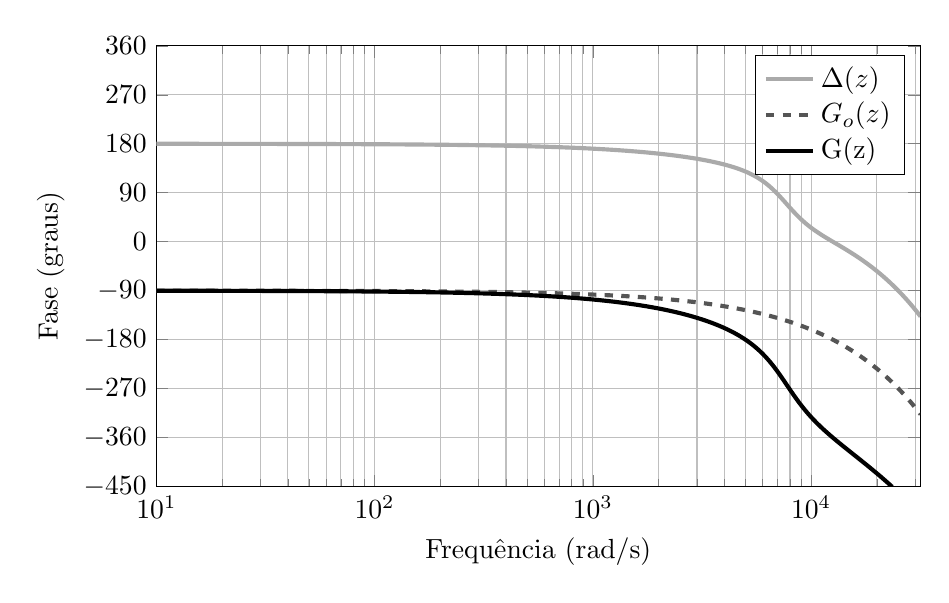
\begin{tikzpicture}

\begin{axis}[%
width=0.8\textwidth,
height=0.461611624834875\textwidth,
scale only axis,
xmode=log,
xmin=10,
xmax=31622.7766016838,
xminorticks=true,
xlabel={Frequência (rad/s)},
xmajorgrids,
xminorgrids,
ymin=-450,
ymax=360,
ytick={-450, -360, -270, -180,  -90,    0,   90,  180,  270,  360},
ylabel={Fase (graus)},
ymajorgrids,
legend style={draw=black,fill=white,legend cell align=left}
]
\addplot [color=mycolor1,solid,line width=1.5pt]
  table[row sep=crcr]{10	179.909684711881\\
10.0461810465159	179.909267626361\\
10.0925753619375	179.908848614695\\
10.139183931163	179.908427667989\\
10.1860077436388	179.908004777305\\
10.2330477933808	179.907579933668\\
10.2803050789954	179.907153128057\\
10.3277806037004	179.906724351411\\
10.375475375347	179.90629359463\\
10.4233904064403	179.905860848567\\
10.4715267141616	179.905426104037\\
10.5198853203895	179.90498935181\\
10.5684672517218	179.904550582615\\
10.6172735394972	179.904109787136\\
10.6663052198171	179.903666956016\\
10.715563333568	179.903222079855\\
10.7650489264432	179.902775149209\\
10.814763048965	179.902326154588\\
10.8647067565072	179.901875086462\\
10.9148811093176	179.901421935255\\
10.9652871725401	179.900966691347\\
11.0159260162376	179.900509345074\\
11.0667987154147	179.900049886727\\
11.1179063500406	179.899588306552\\
11.1692500050717	179.89912459475\\
11.2208307704748	179.898658741477\\
11.2726497412507	179.898190736843\\
11.3247080174565	179.897720570914\\
11.3770067042298	179.897248233708\\
11.4295469118117	179.896773715198\\
11.4823297555707	179.89629700531\\
11.535356356026	179.895818093925\\
11.5886278388715	179.895336970876\\
11.6421453349997	179.894853625948\\
11.6959099805258	179.894368048882\\
11.7499229168114	179.893880229368\\
11.8041852904894	179.893390157051\\
11.8586982534876	179.892897821528\\
11.9134629630538	179.892403212346\\
11.96848058178	179.891906319005\\
12.0237522776272	179.891407130958\\
12.0792792239501	179.890905637606\\
12.135062599522	179.890401828303\\
12.1911035885602	179.889895692355\\
12.2474033807505	179.889387219017\\
12.3039631712731	179.888876397493\\
12.3607841608273	179.888363216941\\
12.4178675556577	179.887847666465\\
12.4752145675793	179.887329735122\\
12.5328264140034	179.886809411916\\
12.5907043179635	179.8862866858\\
12.6488495081411	179.885761545679\\
12.7072632188919	179.885233980404\\
12.765946690272	179.884703978776\\
12.8249011680643	179.884171529542\\
12.8841279038047	179.883636621401\\
12.9436281548089	179.883099242995\\
13.0034031841991	179.882559382918\\
13.0634542609305	179.882017029708\\
13.1237826598188	179.881472171853\\
13.1843896615665	179.880924797784\\
13.2452765527909	179.880374895883\\
13.306444626051	179.879822454475\\
13.3678951798747	179.879267461833\\
13.4296295187868	179.878709906174\\
13.4916489533366	179.878149775663\\
13.5539548001256	179.877587058408\\
13.6165483818355	179.877021742464\\
13.6794310272563	179.876453815829\\
13.7426040713143	179.875883266447\\
13.806068855101	179.875310082206\\
13.8698267259009	179.874734250938\\
13.9338790372205	179.874155760418\\
13.998227148817	179.873574598365\\
14.062872426727	179.872990752443\\
14.1278162432955	179.872404210257\\
14.1930599772055	179.871814959355\\
14.2586050135065	179.871222987228\\
14.3244527436445	179.870628281309\\
14.3906045654914	179.870030828974\\
14.4570618833745	179.869430617538\\
14.5238261081064	179.86882763426\\
14.5908986570152	179.868221866339\\
14.658280953974	179.867613300915\\
14.7259744294318	179.86700192507\\
14.7939805204436	179.866387725825\\
14.8623006707006	179.865770690139\\
14.9309363305612	179.865150804916\\
14.999888957082	179.864528056994\\
15.069160014048	179.863902433154\\
15.1387509720044	179.863273920115\\
15.2086633082875	179.862642504534\\
15.2788985070559	179.862008173006\\
15.3494580593225	179.861370912065\\
15.4203434629857	179.860730708183\\
15.4915562228612	179.860087547769\\
15.5630978507143	179.85944141717\\
15.6349698652918	179.858792302668\\
15.7071737923542	179.858140190484\\
15.779711164708	179.857485066774\\
15.8525835222385	179.856826917631\\
15.9257924119422	179.856165729082\\
15.9993393879601	179.855501487092\\
16.07322601161	179.854834177559\\
16.1474538514202	179.854163786316\\
16.2220244831628	179.853490299133\\
16.2969394898867	179.852813701712\\
16.3722004619516	179.852133979688\\
16.4478089970617	179.851451118634\\
16.5237667002994	179.850765104051\\
16.6000751841599	179.850075921377\\
16.6767360685846	179.849383555981\\
16.7537509809962	179.848687993164\\
16.8311215563331	179.847989218162\\
16.9088494370839	179.847287216139\\
16.9869362733223	179.846581972192\\
17.0653837227424	179.845873471351\\
17.1441934506935	179.845161698574\\
17.2233671302159	179.844446638751\\
17.302906442076	179.843728276702\\
17.3828130748022	179.843006597178\\
17.4630887247206	179.842281584856\\
17.5437350959914	179.841553224348\\
17.6247539006444	179.840821500189\\
17.7061468586161	179.840086396846\\
17.7879156977856	179.839347898713\\
17.8700621540116	179.838605990114\\
17.9525879711692	179.837860655298\\
18.035494901187	179.837111878443\\
18.1187847040838	179.836359643652\\
18.2024591480069	179.835603934956\\
18.2865200092687	179.834844736313\\
18.3709690723849	179.834082031606\\
18.4558081301122	179.833315804642\\
18.5410389834868	179.832546039157\\
18.6266634418617	179.831772718807\\
18.7126833229461	179.830995827178\\
18.7991004528435	179.830215347776\\
18.8859166660905	179.829431264031\\
18.9731338056957	179.8286435593\\
19.060753723179	179.82785221686\\
19.1487782786108	179.82705721991\\
19.2372093406515	179.826258551575\\
19.3260487865912	179.8254561949\\
19.4152985023894	179.824650132851\\
19.5049603827153	179.823840348316\\
19.5950363309877	179.823026824104\\
19.6855282594159	179.822209542945\\
19.7764380890397	179.821388487489\\
19.8677677497706	179.820563640306\\
19.9595191804325	179.819734983885\\
20.0516943288031	179.818902500635\\
20.1442951516552	179.818066172882\\
20.2373236147981	179.817225982873\\
20.3307816931193	179.81638191277\\
20.4246713706267	179.815533944656\\
20.5189946404906	179.814682060528\\
20.6137535050858	179.813826242302\\
20.7089499760343	179.812966471809\\
20.8045860742482	179.812102730799\\
20.900663829972	179.811235000933\\
20.9971852828265	179.810363263792\\
21.0941524818514	179.809487500868\\
21.1915674855492	179.808607693571\\
21.2894323619287	179.807723823223\\
21.387749188549	179.80683587106\\
21.4865200525637	179.805943818232\\
21.5857470507649	179.805047645802\\
21.685432289628	179.804147334743\\
21.7855778853565	179.803242865945\\
21.8861859639264	179.802334220206\\
21.987258661132	179.801421378235\\
22.0887981226306	179.800504320655\\
22.1908065039887	179.799583027997\\
22.2932859707273	179.798657480703\\
22.396238698368	179.797727659124\\
22.499666872479	179.796793543522\\
22.603572688722	179.795855114065\\
22.7079583528983	179.794912350832\\
22.8128260809959	179.793965233808\\
22.9181780992365	179.793013742889\\
23.0240166441225	179.792057857873\\
23.130343962485	179.791097558468\\
23.237162311531	179.790132824289\\
23.3444739588916	179.789163634855\\
23.4522811826701	179.788189969591\\
23.5605862714901	179.787211807827\\
23.6693915245447	179.786229128797\\
23.7786992516445	179.78524191164\\
23.8885117732672	179.784250135398\\
23.9988314206069	179.783253779018\\
24.1096605356231	179.782252821346\\
24.2210014710909	179.781247241134\\
24.3328565906507	179.780237017034\\
24.4452282688584	179.779222127599\\
24.558118891236	179.778202551286\\
24.6715308543219	179.777178266449\\
24.7854665657221	179.776149251343\\
24.899928444161	179.775115484123\\
25.0149189195332	179.774076942844\\
25.1304404329547	179.773033605458\\
25.2464954368146	179.771985449815\\
25.3630863948276	179.770932453666\\
25.4802157820863	179.769874594654\\
25.597886085113	179.768811850324\\
25.7160998019135	179.767744198113\\
25.8348594420295	179.766671615357\\
25.9541675265918	179.765594079285\\
26.0740265883745	179.764511567023\\
26.194439171848	179.763424055589\\
26.3154078332332	179.762331521896\\
26.4369351405564	179.761233942752\\
26.5590236737027	179.760131294855\\
26.6816760244719	179.759023554798\\
26.8048947966327	179.757910699063\\
26.9286826059784	179.756792704025\\
27.0530420803822	179.755669545952\\
27.1779758598533	179.754541200998\\
27.3034865965925	179.753407645211\\
27.4295769550488	179.752268854525\\
27.556249611976	179.751124804766\\
27.6835072564894	179.749975471645\\
27.8113525901229	179.748820830764\\
27.9397883268864	179.74766085761\\
28.0688171933232	179.746495527559\\
28.1984419285683	179.745324815871\\
28.3286652844062	179.744148697693\\
28.4594900253294	179.742967148056\\
28.5909189285972	179.741780141879\\
28.7229547842946	179.74058765396\\
28.8556003953913	179.739389658986\\
28.9888585778017	179.738186131523\\
29.1227321604441	179.736977046022\\
29.2572239853012	179.735762376814\\
29.3923369074803	179.734542098113\\
29.5280737952738	179.733316184013\\
29.6644375302202	179.73208460849\\
29.8014310071653	179.730847345398\\
29.9390571343235	179.729604368471\\
30.0773188333397	179.728355651321\\
30.2162190393513	179.727101167439\\
30.3557607010504	179.725840890194\\
30.4959467807464	179.72457479283\\
30.6367802544292	179.72330284847\\
30.7782641118319	179.72202503011\\
30.9204013564946	179.720741310625\\
31.063195005828	179.719451662761\\
31.2066480911777	179.71815605914\\
31.350763657888	179.716854472257\\
31.4955447653674	179.715546874482\\
31.6409944871527	179.714233238054\\
31.7871159109747	179.712913535085\\
31.9339121388238	179.711587737561\\
32.0813862870155	179.710255817334\\
32.229541486257	179.708917746129\\
32.3783808817133	179.70757349554\\
32.5279076330741	179.70622303703\\
32.6781249146208	179.704866341928\\
32.8290359152942	179.703503381434\\
32.9806438387618	179.702134126613\\
33.132951903486	179.700758548396\\
33.2859633427924	179.699376617582\\
33.4396814049384	179.697988304831\\
33.5941093531822	179.696593580672\\
33.7492504658521	179.695192415495\\
33.9051080364161	179.693784779556\\
34.0616853735517	179.692370642969\\
34.2189858012163	179.690949975715\\
34.3770126587175	179.689522747634\\
34.5357693007845	179.688088928425\\
34.6952590976386	179.686648487652\\
34.8554854350656	179.685201394732\\
35.0164517144866	179.683747618947\\
35.1781613530314	179.682287129433\\
35.3406177836102	179.680819895185\\
35.5038244549868	179.679345885054\\
35.6677848318515	179.677865067749\\
35.8325023948954	179.676377411831\\
35.9979806408833	179.67488288572\\
36.1642230827288	179.673381457688\\
36.3312332495683	179.671873095859\\
36.4990146868361	179.670357768213\\
36.6675709563398	179.66883544258\\
36.8369056363357	179.667306086642\\
37.007022321605	179.665769667931\\
37.1779246235299	179.66422615383\\
37.3496161701703	179.662675511572\\
37.5221006063408	179.661117708236\\
37.6953815936883	179.659552710753\\
37.8694628107696	179.657980485897\\
38.0443479531292	179.656401000292\\
38.2200407333782	179.654814220405\\
38.3965448812729	179.653220112551\\
38.5738641437941	179.651618642887\\
38.7520022852263	179.650009777414\\
38.9309630872381	179.648393481979\\
39.1107503489621	179.646769722266\\
39.2913678870758	179.645138463805\\
39.4728195358824	179.643499671966\\
39.6551091473924	179.641853311956\\
39.8382405914052	179.640199348826\\
40.0222177555915	179.638537747461\\
40.2070445455755	179.636868472588\\
40.3927248850181	179.635191488768\\
40.5792627157	179.633506760399\\
40.7666619976054	179.631814251717\\
40.9549267090063	179.630113926788\\
41.1440608465467	179.628405749517\\
41.3340684253274	179.626689683639\\
41.5249534789915	179.624965692724\\
41.7167200598098	179.623233740171\\
41.9093722387671	179.621493789212\\
42.1029141056481	179.619745802909\\
42.2973497691249	179.617989744152\\
42.4926833568435	179.616225575662\\
42.6889190155123	179.614453259985\\
42.8860609109892	179.612672759496\\
43.0841132283705	179.610884036395\\
43.2830801720801	179.609087052709\\
43.4829659659579	179.607281770289\\
43.6837748533501	179.605468150809\\
43.8855110971994	179.603646155767\\
44.0881789801347	179.601815746481\\
44.2917828045629	179.599976884094\\
44.4963268927599	179.598129529567\\
44.701815586962	179.59627364368\\
44.9082532494586	179.594409187035\\
45.1156442626847	179.59253612005\\
45.3239930293136	179.590654402959\\
45.5333039723509	179.588763995815\\
45.7435815352278	179.586864858484\\
45.954830181896	179.584956950649\\
46.167054396922	179.583040231805\\
46.3802586855826	179.581114661261\\
46.5944475739604	179.579180198137\\
46.8096256090399	179.577236801366\\
47.0257973588042	179.575284429689\\
47.2429674123316	179.573323041658\\
47.4611403798933	179.571352595633\\
47.6803208930514	179.569373049783\\
47.9005136047569	179.567384362081\\
48.1217231894485	179.565386490308\\
48.3439543431522	179.56337939205\\
48.5672117835806	179.561363024697\\
48.791500250233	179.559337345441\\
49.0168245044966	179.557302311278\\
49.243189329747	179.555257879004\\
49.4705995314498	179.553204005216\\
49.6990599372628	179.551140646311\\
49.9285753971387	179.549067758483\\
50.1591507834275	179.546985297727\\
50.3907909909802	179.54489321983\\
50.6235009372529	179.542791480379\\
50.8572855624109	179.540680034754\\
51.0921498294339	179.538558838129\\
51.3280987242209	179.536427845472\\
51.5651372556965	179.534287011541\\
51.8032704559168	179.532136290886\\
52.0425033801768	179.529975637849\\
52.2828411071172	179.527805006557\\
52.5242887388322	179.52562435093\\
52.7668514009784	179.523433624671\\
53.010534242883	179.521232781271\\
53.2553424376533	179.519021774008\\
53.5012811822866	179.516800555939\\
53.7483556977805	179.51456907991\\
53.9965712292437	179.512327298547\\
54.2459330460073	179.510075164254\\
54.4964464417369	179.507812629221\\
54.7481167345445	179.505539645412\\
55.0009492671021	179.503256164573\\
55.2549494067543	179.500962138225\\
55.510122545633	179.498657517666\\
55.7664741007712	179.496342253967\\
56.0240095142187	179.494016297976\\
56.282734253157	179.491679600312\\
56.5426538100157	179.489332111367\\
56.8037737025889	179.486973781304\\
57.0660994741527	179.484604560054\\
57.3296366935823	179.482224397318\\
57.5943909554708	179.479833242565\\
57.8603678802477	179.477431045031\\
58.1275731142982	179.475017753716\\
58.3960123300829	179.472593317385\\
58.6656912262587	179.470157684567\\
58.9366155277994	179.467710803553\\
59.2087909861172	179.465252622395\\
59.4822233791852	179.462783088905\\
59.7569185116595	179.460302150653\\
60.0328822150028	179.45780975497\\
60.3101203476082	179.45530584894\\
60.5886387949234	179.452790379404\\
60.8684434695757	179.450263292959\\
61.1495403114975	179.447724535953\\
61.4319352880526	179.445174054488\\
61.7156343941624	179.442611794415\\
62.0006436524339	179.440037701337\\
62.2869691132868	179.437451720604\\
62.5746168550822	179.434853797316\\
62.8635929842521	179.432243876317\\
63.1539036354283	179.429621902197\\
63.445554971573	179.42698781929\\
63.7385531841099	179.424341571674\\
64.032904493055	179.421683103167\\
64.3286151471491	179.419012357328\\
64.6256914239905	179.416329277457\\
64.9241396301678	179.413633806589\\
65.2239661013943	179.410925887498\\
65.5251772026422	179.408205462693\\
65.827779328278	179.405472474419\\
66.1317789021976	179.402726864652\\
66.4371823779638	179.399968575101\\
66.7439962389419	179.397197547205\\
67.0522269984386	179.394413722135\\
67.3618811998395	179.391617040786\\
67.6729654167483	179.388807443784\\
67.9854862531262	179.385984871479\\
68.2994503434323	179.383149263945\\
68.6148643527643	179.38030056098\\
68.931734977	179.377438702105\\
69.2500689429393	179.374563626559\\
69.5698730084476	179.371675273302\\
69.8911539625984	179.368773581013\\
70.213918625818	179.365858488084\\
70.5381738500302	179.362929932628\\
70.8639265188016	179.359987852467\\
71.191183547488	179.357032185139\\
71.5199518833808	179.354062867891\\
71.8502385058548	179.351079837683\\
72.1820504265165	179.348083031182\\
72.5153946893524	179.345072384763\\
72.8502783708792	179.342047834506\\
73.1867085802933	179.339009316197\\
73.5246924596224	179.335956765326\\
73.8642371838769	179.332890117083\\
74.2053499612018	179.329809306359\\
74.5480380330304	179.326714267746\\
74.8923086742377	179.323604935533\\
75.2381691932944	179.320481243705\\
75.585626932423	179.317343125942\\
75.9346892677529	179.314190515618\\
76.2853636094773	179.3110233458\\
76.6376574020103	179.307841549243\\
76.9915781241455	179.304645058395\\
77.3471332892138	179.30143380539\\
77.7043304452438	179.29820772205\\
78.0631771751216	179.294966739878\\
78.4236810967518	179.291710790067\\
78.7858498632195	179.288439803486\\
79.1496911629522	179.285153710688\\
79.5152127198837	179.281852441905\\
79.8824222936175	179.278535927046\\
80.2513276795919	179.275204095696\\
80.6219367092452	179.271856877116\\
80.9942572501823	179.268494200239\\
81.3682972063414	179.26511599367\\
81.7440645181619	179.261722185685\\
82.121567162753	179.258312704226\\
82.5008131540631	179.254887476907\\
82.8818105430498	179.251446431002\\
83.2645674178507	179.247989493454\\
83.6490919039556	179.244516590864\\
84.0353921643786	179.241027649499\\
84.423476399831	179.23752259528\\
84.8133528488963	179.23400135379\\
85.2050297882047	179.230463850265\\
85.5985155326084	179.226910009599\\
85.9938184353586	179.223339756337\\
86.3909468882829	179.219753014675\\
86.7899093219629	179.216149708459\\
87.1907142059136	179.212529761185\\
87.5933700487633	179.208893095994\\
87.9978853984339	179.205239635672\\
88.4042688423224	179.201569302649\\
88.8125290074835	179.197882018995\\
89.2226745608124	179.194177706421\\
89.6347142092288	179.190456286279\\
90.0486566998624	179.186717679552\\
90.4645108202374	179.182961806864\\
90.88228539846	179.179188588467\\
91.3019893034057	179.175397944249\\
91.7236314449071	179.171589793724\\
92.1472207739435	179.167764056037\\
92.5727662828307	179.163920649959\\
93.0002770054119	179.160059493884\\
93.4297620172496	179.156180505832\\
93.8612304358183	179.152283603441\\
94.2946914206979	179.148368703971\\
94.730154173768	179.144435724298\\
95.1676279394036	179.140484580915\\
95.6071220046713	179.136515189929\\
96.0486456995261	179.132527467059\\
96.4922083970099	179.128521327636\\
96.9378195134503	179.124496686597\\
97.3854885086602	179.12045345849\\
97.8352248861393	179.116391557465\\
98.2870381932753	179.112310897275\\
98.7409380215466	179.108211391279\\
99.1969340067261	179.10409295243\\
99.655035829086	179.099955493282\\
100.115253213603	179.095798925985\\
100.577595930163	179.091623162283\\
101.042073793774	179.08742811351\\
101.508696664767	179.083213690594\\
101.977474449012	179.078979804049\\
102.448417098122	179.074726363977\\
102.921534609671	179.070453280062\\
103.3968370274	179.066160461573\\
103.874334441436	179.061847817361\\
104.354036988501	179.057515255853\\
104.83595485213	179.053162685054\\
105.320098262886	179.048790012544\\
105.80647749858	179.044397145476\\
106.295102884484	179.039983990575\\
106.785984793556	179.035550454133\\
107.279133646656	179.031096442011\\
107.774559912768	179.026621859634\\
108.272274109224	179.02212661199\\
108.772286801926	179.017610603627\\
109.27460860557	179.013073738655\\
109.779250183872	179.008515920738\\
110.286222249794	179.003937053097\\
110.795535565772	178.999337038503\\
111.307200943943	178.994715779281\\
111.821229246378	178.990073177302\\
112.337631385307	178.985409133986\\
112.856418323356	178.980723550296\\
113.377601073777	178.976016326737\\
113.901190700682	178.971287363355\\
114.427198319278	178.966536559734\\
114.955635096105	178.961763814995\\
115.486512249268	178.95696902779\\
116.019841048683	178.952152096307\\
116.555632816306	178.947312918259\\
117.093898926384	178.94245139089\\
117.634650805689	178.937567410966\\
118.177899933763	178.932660874779\\
118.723657843162	178.927731678139\\
119.271936119701	178.922779716378\\
119.822746402699	178.91780488434\\
120.376100385228	178.912807076387\\
120.932009814357	178.90778618639\\
121.490486491407	178.902742107731\\
122.051542272196	178.897674733299\\
122.615189067297	178.892583955488\\
123.181438842284	178.887469666195\\
123.750303617991	178.882331756817\\
124.321795470765	178.87717011825\\
124.895926532723	178.871984640883\\
125.472708992008	178.866775214603\\
126.052155093052	178.861541728784\\
126.63427713683	178.856284072292\\
127.219087481126	178.851002133476\\
127.806598540793	178.845695800172\\
128.396822788018	178.840364959696\\
128.989772752585	178.835009498845\\
129.585461022141	178.82962930389\\
130.183900242466	178.824224260578\\
130.785103117737	178.818794254129\\
131.389082410804	178.81333916923\\
131.995850943453	178.807858890038\\
132.605421596686	178.802353300173\\
133.217807310988	178.796822282716\\
133.833021086605	178.791265720209\\
134.451075983821	178.785683494652\\
135.071985123233	178.780075487499\\
135.69576168603	178.774441579654\\
136.322418914273	178.768781651473\\
136.951970111177	178.763095582759\\
137.584428641392	178.757383252757\\
138.219807931287	178.751644540158\\
138.858121469236	178.745879323087\\
139.499382805904	178.740087479111\\
140.143605554534	178.734268885228\\
140.790803391236	178.728423417868\\
141.440990055278	178.72255095289\\
142.094179349378	178.716651365579\\
142.750385139995	178.710724530643\\
143.409621357626	178.704770322213\\
144.0719019971	178.698788613836\\
144.737241117876	178.692779278476\\
145.405652844341	178.686742188507\\
146.077151366109	178.680677215717\\
146.751750938323	178.674584231298\\
147.42946588196	178.668463105849\\
148.110310584131	178.66231370937\\
148.794299498388	178.656135911259\\
149.481447145032	178.649929580311\\
150.171768111418	178.643694584715\\
150.865277052271	178.63743079205\\
151.561988689989	178.631138069283\\
152.261917814963	178.624816282767\\
152.965079285884	178.618465298235\\
153.671488030065	178.612084980802\\
154.381159043753	178.605675194956\\
155.094107392451	178.599235804562\\
155.810348211234	178.592766672853\\
156.529896705074	178.586267662432\\
157.25276814916	178.579738635265\\
157.978977889225	178.57317945268\\
158.708541341869	178.566589975365\\
159.441473994887	178.559970063362\\
160.177791407599	178.553319576069\\
160.917509211179	178.54663837223\\
161.66064310899	178.53992630994\\
162.40720887691	178.533183246634\\
163.157222363676	178.526409039091\\
163.910699491214	178.519603543425\\
164.66765625498	178.512766615088\\
165.428108724297	178.50589810886\\
166.192073042701	178.498997878852\\
166.959565428276	178.492065778501\\
167.730602174008	178.485101660563\\
168.505199648122	178.478105377117\\
169.283374294433	178.471076779555\\
170.065142632699	178.464015718583\\
170.850521258965	178.456922044217\\
171.639526845917	178.449795605779\\
172.432176143241	178.442636251895\\
173.228485977972	178.435443830489\\
174.028473254854	178.428218188785\\
174.832154956701	178.420959173296\\
175.639548144754	178.413666629829\\
176.450669959044	178.406340403477\\
177.265537618758	178.398980338616\\
178.084168422602	178.391586278902\\
178.906579749169	178.384158067269\\
179.732789057308	178.376695545923\\
180.562813886497	178.369198556343\\
181.39667185721	178.361666939272\\
182.234380671297	178.354100534717\\
183.075958112354	178.346499181947\\
183.921422046107	178.338862719485\\
184.770790420785	178.331190985109\\
185.624081267505	178.323483815845\\
186.481312700654	178.315741047966\\
187.342502918271	178.307962516989\\
188.207670202438	178.300148057668\\
189.076832919665	178.292297503994\\
189.950009521279	178.28441068919\\
190.827218543818	178.276487445706\\
191.708478609426	178.268527605219\\
192.593808426241	178.260530998627\\
193.483226788801	178.252497456043\\
194.376752578439	178.244426806799\\
195.274404763682	178.236318879433\\
196.176202400658	178.228173501692\\
197.082164633495	178.219990500526\\
197.992310694735	178.211769702084\\
198.906659905733	178.20351093171\\
199.825231677076	178.195214013942\\
200.748045508988	178.186878772503\\
201.675120991751	178.178505030304\\
202.606477806113	178.170092609433\\
203.542135723711	178.161641331159\\
204.482114607491	178.15315101592\\
205.426434412127	178.144621483326\\
206.375115184445	178.136052552151\\
207.32817706385	178.12744404033\\
208.285640282755	178.118795764956\\
209.247525167004	178.110107542277\\
210.213852136311	178.101379187688\\
211.18464170469	178.092610515732\\
212.159914480891	178.083801340093\\
213.139691168835	178.074951473592\\
214.123992568061	178.066060728185\\
215.112839574156	178.057128914957\\
216.10625317921	178.048155844119\\
217.104254472254	178.039141325003\\
218.106864639713	178.030085166059\\
219.114104965849	178.020987174851\\
220.12599683322	178.011847158051\\
221.142561723131	178.002664921437\\
222.163821216089	177.993440269888\\
223.189796992262	177.98417300738\\
224.220510831939	177.974862936981\\
225.255984615994	177.965509860848\\
226.296240326348	177.956113580221\\
227.341300046436	177.946673895422\\
228.391185961678	177.937190605846\\
229.44592035995	177.927663509962\\
230.505525632052	177.918092405303\\
231.570024272191	177.908477088468\\
232.639438878451	177.898817355112\\
233.713792153278	177.889112999944\\
234.793106903962	177.879363816723\\
235.877406043117	177.869569598254\\
236.966712589169	177.859730136381\\
238.061049666849	177.849845221984\\
239.160440507677	177.839914644977\\
240.264908450462	177.829938194298\\
241.374476941791	177.81991565791\\
242.48916953653	177.809846822794\\
243.609009898327	177.799731474942\\
244.734021800108	177.789569399359\\
245.864229124585	177.77936038005\\
246.999655864764	177.769104200022\\
248.140326124455	177.758800641277\\
249.286264118777	177.748449484807\\
250.437494174681	177.738050510589\\
251.594040731461	177.727603497582\\
252.755928341275	177.717108223719\\
253.923181669665	177.706564465907\\
255.09582549608	177.695972000017\\
256.273884714404	177.685330600885\\
257.457384333485	177.6746400423\\
258.646349477661	177.663900097005\\
259.840805387301	177.65311053669\\
261.040777419332	177.642271131988\\
262.246291047787	177.631381652467\\
263.457371864337	177.62044186663\\
264.674045578839	177.609451541905\\
265.896338019882	177.598410444645\\
267.124275135332	177.587318340116\\
268.357882992886	177.576174992501\\
269.597187780627	177.564980164886\\
270.842215807572	177.553733619263\\
272.092993504239	177.542435116518\\
273.349547423206	177.531084416429\\
274.611904239671	177.519681277662\\
275.880090752022	177.508225457764\\
277.154133882405	177.496716713156\\
278.434060677294	177.485154799134\\
279.719898308069	177.473539469856\\
281.011674071587	177.461870478342\\
282.309415390768	177.450147576466\\
283.613149815172	177.438370514952\\
284.922905021585	177.42653904337\\
286.238708814609	177.414652910126\\
287.560589127251	177.402711862461\\
288.888574021513	177.390715646443\\
290.222691688993	177.378664006965\\
291.562970451479	177.366556687733\\
292.909438761552	177.354393431268\\
294.262125203191	177.342173978895\\
295.621058492378	177.329898070739\\
296.98626747771	177.317565445721\\
298.357781141006	177.305175841551\\
299.735628597932	177.29272899472\\
301.119839098607	177.280224640499\\
302.510442028234	177.26766251293\\
303.907466907719	177.255042344822\\
305.310943394298	177.242363867742\\
306.720901282168	177.229626812016\\
308.137370503119	177.216830906713\\
309.560381127168	177.20397587965\\
310.989963363199	177.191061457377\\
312.426147559604	177.178087365177\\
313.868964204927	177.165053327059\\
315.318443928511	177.15195906575\\
316.774617501149	177.138804302688\\
318.237515835737	177.125588758021\\
319.707169987928	177.112312150597\\
321.183611156796	177.098974197959\\
322.666870685493	177.085574616338\\
324.156980061919	177.072113120649\\
325.653970919389	177.058589424481\\
327.1578750373	177.045003240096\\
328.668724341813	177.031354278417\\
330.186550906528	177.017642249028\\
331.711386953162	177.00386686016\\
333.243264852235	176.990027818693\\
334.78221712376	176.976124830144\\
336.328276437929	176.962157598662\\
337.881475615808	176.948125827022\\
339.441847630035	176.934029216617\\
341.009425605519	176.919867467454\\
342.584242820144	176.905640278148\\
344.166332705473	176.89134734591\\
345.75572884746	176.876988366546\\
347.352464987164	176.86256303445\\
348.956575021463	176.848071042592\\
350.568093003772	176.833512082518\\
352.187053144771	176.81888584434\\
353.813489813129	176.804192016728\\
355.447437536229	176.789430286907\\
357.088931000911	176.774600340646\\
358.738005054198	176.759701862254\\
360.39469470404	176.744734534572\\
362.059035120061	176.729698038968\\
363.731061634299	176.714592055324\\
365.410809741959	176.699416262038\\
367.09831510217	176.684170336009\\
368.793613538734	176.668853952635\\
370.496741040893	176.653466785804\\
372.207733764093	176.638008507885\\
373.926628030746	176.622478789725\\
375.653460331008	176.606877300638\\
377.388267323548	176.591203708401\\
379.13108583633	176.575457679243\\
380.881952867393	176.55963887784\\
382.640905585636	176.54374696731\\
384.407981331609	176.527781609198\\
386.183217618305	176.511742463479\\
387.966652131954	176.49562918854\\
389.758322732826	176.479441441181\\
391.558267456034	176.463178876603\\
393.366524512341	176.446841148399\\
395.183132288971	176.430427908553\\
397.008129350424	176.413938807424\\
398.841554439296	176.397373493745\\
400.683446477099	176.380731614612\\
402.533844565089	176.364012815475\\
404.392787985098	176.347216740135\\
406.260316200361	176.330343030731\\
408.136468856361	176.313391327736\\
410.021285781671	176.296361269944\\
411.914806988789	176.279252494469\\
413.817072675003	176.262064636731\\
415.72812322323	176.244797330451\\
417.647999202884	176.227450207643\\
419.576741370729	176.210022898603\\
421.514390671752	176.192515031903\\
423.460988240025	176.174926234385\\
425.416575399583	176.157256131147\\
427.381193665299	176.13950434554\\
429.354884743766	176.121670499157\\
431.337690534184	176.103754211825\\
433.329653129246	176.085755101597\\
435.330814816033	176.067672784742\\
437.341218076915	176.049506875739\\
439.360905590448	176.031256987268\\
441.389920232282	176.012922730198\\
443.428305076071	175.994503713581\\
445.476103394389	175.975999544646\\
447.533358659646	175.957409828784\\
449.600114545014	175.938734169544\\
451.67641492535	175.919972168623\\
453.762303878129	175.901123425854\\
455.857825684385	175.882187539204\\
457.963024829641	175.863164104757\\
460.077946004862	175.844052716711\\
462.202634107401	175.824852967366\\
464.33713424195	175.805564447114\\
466.481491721497	175.786186744434\\
468.635752068297	175.766719445878\\
470.799961014824	175.747162136064\\
472.974164504755	175.727514397667\\
475.158408693936	175.707775811408\\
477.352739951367	175.687945956046\\
479.557204860185	175.66802440837\\
481.771850218653	175.648010743183\\
483.996723041153	175.627904533302\\
486.231870559183	175.607705349539\\
488.477340222363	175.587412760698\\
490.73317969944	175.567026333562\\
492.999436879299	175.546545632884\\
495.276159871982	175.525970221378\\
497.563397009708	175.505299659706\\
499.861196847899	175.484533506472\\
502.169608166212	175.46367131821\\
504.48867996957	175.442712649374\\
506.818461489212	175.421657052327\\
509.159002183727	175.400504077333\\
511.51035174011	175.379253272544\\
513.872560074817	175.357904183994\\
516.245677334823	175.336456355583\\
518.629753898685	175.31490932907\\
521.024840377617	175.293262644063\\
523.430987616559	175.271515838007\\
525.848246695256	175.249668446171\\
528.27666892935	175.227720001646\\
530.716305871459	175.205670035322\\
533.167209312278	175.183518075887\\
535.629431281677	175.161263649813\\
538.103024049808	175.138906281344\\
540.588040128206	175.116445492484\\
543.084532270915	175.093880802992\\
545.592553475602	175.071211730362\\
548.11215698468	175.048437789821\\
550.643396286443	175.025558494309\\
553.186325116201	175.002573354476\\
555.740997457415	174.979481878664\\
558.307467542852	174.956283572898\\
560.885789855729	174.932977940878\\
563.476019130871	174.90956448396\\
566.078210355879	174.88604270115\\
568.692418772287	174.862412089094\\
571.318699876742	174.838672142058\\
573.957109422183	174.814822351924\\
576.607703419019	174.790862208175\\
579.27053813632	174.766791197884\\
581.945670103016	174.7426088057\\
584.633156109091	174.718314513837\\
587.333053206791	174.693907802063\\
590.045418711838	174.669388147686\\
592.77031020464	174.644755025544\\
595.507785531519	174.620007907988\\
598.25790280594	174.595146264874\\
601.020720409738	174.57016956355\\
603.796296994364	174.54507726884\\
606.584691482126	174.519868843035\\
609.385963067442	174.494543745877\\
612.200171218097	174.469101434549\\
615.027375676503	174.443541363661\\
617.867636460969	174.417862985236\\
620.721013866976	174.392065748697\\
623.587568468455	174.366149100857\\
626.467361119072	174.340112485899\\
629.360452953524	174.31395534537\\
632.266905388836	174.287677118162\\
635.186780125658	174.261277240503\\
638.120139149584	174.234755145939\\
641.067044732464	174.208110265321\\
644.027559433723	174.181342026797\\
647.001746101695	174.154449855788\\
649.989667874954	174.127433174984\\
652.991388183652	174.100291404322\\
656.00697075087	174.073023960978\\
659.03647959397	174.045630259347\\
662.07997902595	174.018109711033\\
665.137533656814	173.990461724834\\
668.209208394941	173.962685706725\\
671.295068448464	173.934781059845\\
674.395179326655	173.906747184482\\
677.509606841313	173.878583478058\\
680.638417108163	173.850289335115\\
683.78167654826	173.821864147298\\
686.9394518894	173.793307303341\\
690.11181016753	173.764618189052\\
693.298818728181	173.735796187297\\
696.500545227891	173.706840677985\\
699.717057635642	173.67775103805\\
702.948424234306	173.64852664144\\
706.19471362209	173.619166859098\\
709.455994713995	173.589671058945\\
712.732336743282	173.560038605867\\
716.023809262934	173.530268861697\\
719.330482147139	173.500361185198\\
722.652425592773	173.470314932048\\
725.989710120886	173.440129454824\\
729.3424065782	173.409804102983\\
732.71058613862	173.379338222848\\
736.094320304735	173.348731157589\\
739.493680909343	173.317982247207\\
742.908740116972	173.287090828515\\
746.339570425412	173.256056235125\\
749.786244667258	173.224877797425\\
753.248836011454	173.193554842566\\
756.727417964843	173.162086694441\\
760.222064373731	173.130472673673\\
763.732849425456	173.098712097586\\
767.259847649959	173.0668042802\\
770.803133921369	173.034748532203\\
774.362783459591	173.002544160938\\
777.938871831903	172.97019047038\\
781.531474954562	172.937686761122\\
785.140669094413	172.905032330354\\
788.76653087051	172.872226471844\\
792.40913725574	172.839268475918\\
796.068565578463	172.806157629443\\
799.744893524145	172.772893215805\\
803.438199137013	172.739474514892\\
807.148560821713	172.705900803073\\
810.876057344967	172.672171353175\\
814.620767837254	172.638285434471\\
818.382771794484	172.60424231265\\
822.162149079689	172.570041249803\\
825.958979924714	172.535681504402\\
829.773344931927	172.501162331276\\
833.605325075921	172.466482981593\\
837.455001705243	172.431642702837\\
841.322456544116	172.396640738787\\
845.207771694168	172.361476329497\\
849.111029636188	172.326148711273\\
853.032313231867	172.290657116652\\
856.971705725559	172.255000774378\\
860.92929074605	172.219178909381\\
864.905152308334	172.183190742756\\
868.899374815392	172.147035491737\\
872.91204305999	172.110712369678\\
876.943242226474	172.074220586027\\
880.993057892579	172.037559346302\\
885.061576031251	172.00072785207\\
889.148883012464	171.963725300924\\
893.255065605058	171.926550886456\\
897.380210978585	171.889203798232\\
901.52440670515	171.851683221774\\
905.687740761275	171.813988338527\\
909.870301529772	171.776118325841\\
914.07217780161	171.738072356941\\
918.293458777803	171.699849600904\\
922.534234071309	171.661449222634\\
926.794593708924	171.622870382835\\
931.074628133199	171.584112237983\\
935.374428204358	171.545173940303\\
939.694085202226	171.506054637741\\
944.033690828168	171.466753473937\\
948.39333720704	171.427269588197\\
952.773116889131	171.387602115465\\
957.173122852146	171.3477501863\\
961.593448503166	171.307712926842\\
966.034187680636	171.267489458784\\
970.495434656357	171.22707889935\\
974.977284137491	171.186480361258\\
979.479831268559	171.145692952694\\
984.003171633478	171.104715777285\\
988.547401257578	171.063547934064\\
993.112616609642	171.022188517444\\
997.698914603958	170.980636617185\\
1002.30639260238	170.938891318364\\
1006.93514841637	170.896951701345\\
1011.58528030912	170.854816841744\\
1016.2568869976	170.812485810401\\
1020.95006765465	170.769957673343\\
1025.66492191112	170.727231491759\\
1030.40154985798	170.684306321957\\
1035.16005204838	170.64118121534\\
1039.94052949988	170.597855218364\\
1044.74308369654	170.554327372512\\
1049.56781659108	170.510596714252\\
1054.41483060703	170.466662275006\\
1059.28422864096	170.422523081113\\
1064.17611406461	170.378178153796\\
1069.09059072708	170.333626509121\\
1074.02776295708	170.288867157966\\
1078.98773556513	170.243899105977\\
1083.97061384575	170.198721353536\\
1088.97650357974	170.153332895723\\
1094.00551103639	170.107732722271\\
1099.05774297578	170.061919817534\\
1104.13330665098	170.015893160447\\
1109.2323098104	169.969651724479\\
1114.35486070002	169.923194477602\\
1119.50106806574	169.876520382243\\
1124.67104115564	169.829628395244\\
1129.86488972231	169.782517467823\\
1135.0827240252	169.735186545527\\
1140.32465483296	169.687634568191\\
1145.59079342577	169.639860469895\\
1150.8812515977	169.591863178918\\
1156.19614165913	169.543641617693\\
1161.53557643908	169.495194702764\\
1166.89966928762	169.446521344735\\
1172.28853407829	169.397620448228\\
1177.70228521052	169.348490911833\\
1183.14103761204	169.299131628062\\
1188.60490674132	169.249541483296\\
1194.09400859005	169.19971935774\\
1199.60845968555	169.149664125371\\
1205.14837709331	169.099374653888\\
1210.71387841942	169.048849804659\\
1216.30508181309	168.998088432668\\
1221.92210596917	168.947089386467\\
1227.56507013062	168.895851508116\\
1233.23409409112	168.844373633131\\
1238.92929819754	168.792654590431\\
1244.65080335254	168.740693202277\\
1250.3987310171	168.688488284218\\
1256.17320321316	168.636038645035\\
1261.97434252612	168.583343086676\\
1267.80227210752	168.530400404204\\
1273.65711567764	168.47720938573\\
1279.53899752808	168.423768812357\\
1285.44804252445	168.370077458113\\
1291.38437610901	168.316134089891\\
1297.34812430331	168.261937467384\\
1303.33941371088	168.207486343017\\
1309.35837151994	168.152779461887\\
1315.40512550606	168.097815561687\\
1321.47980403488	168.042593372645\\
1327.58253606487	167.987111617453\\
1333.71345115004	167.931369011194\\
1339.87267944269	167.875364261271\\
1346.06035169616	167.819096067336\\
1352.27659926764	167.762563121216\\
1358.52155412096	167.705764106834\\
1364.79534882933	167.648697700138\\
1371.09811657822	167.59136256902\\
1377.42999116818	167.533757373237\\
1383.79110701763	167.475880764332\\
1390.18159916578	167.417731385553\\
1396.60160327544	167.359307871769\\
1403.05125563594	167.300608849385\\
1409.53069316601	167.241632936256\\
1416.04005341668	167.182378741605\\
1422.5794745742	167.122844865928\\
1429.14909546299	167.063029900904\\
1435.74905554856	167.00293242931\\
1442.3794949405	166.942551024921\\
1449.04055439544	166.881884252417\\
1455.73237532004	166.820930667288\\
1462.45509977397	166.759688815735\\
1469.20887047298	166.698157234568\\
1475.99383079187	166.636334451108\\
1482.81012476756	166.574218983081\\
1489.65789710218	166.511809338513\\
1496.53729316606	166.449104015625\\
1503.44845900091	166.386101502721\\
1510.39154132284	166.322800278077\\
1517.36668752555	166.25919880983\\
1524.37404568338	166.195295555863\\
1531.41376455451	166.131088963686\\
1538.4859935841	166.066577470318\\
1545.59088290748	166.001759502163\\
1552.72858335329	165.936633474892\\
1559.89924644673	165.871197793309\\
1567.10302441275	165.805450851231\\
1574.34007017931	165.73939103135\\
1581.61053738059	165.673016705105\\
1588.91458036027	165.606326232545\\
1596.25235417481	165.539317962187\\
1603.62401459674	165.471990230882\\
1611.02971811795	165.404341363666\\
1618.46962195303	165.336369673616\\
1625.94388404263	165.268073461701\\
1633.45266305675	165.19945101663\\
1640.99611839816	165.130500614695\\
1648.57441020578	165.061220519619\\
1656.18769935804	164.991608982389\\
1663.83614747635	164.921664241095\\
1671.51991692849	164.851384520763\\
1679.23917083208	164.780768033185\\
1686.99407305804	164.709812976741\\
1694.78478823403	164.63851753623\\
1702.61148174801	164.566879882681\\
1710.47431975172	164.494898173175\\
1718.37346916419	164.422570550653\\
1726.30909767531	164.349895143728\\
1734.28137374936	164.276870066485\\
1742.29046662864	164.203493418286\\
1750.33654633699	164.129763283566\\
1758.41978368348	164.055677731622\\
1766.54035026596	163.981234816407\\
1774.69841847474	163.906432576309\\
1782.89416149627	163.831269033933\\
1791.12775331676	163.755742195877\\
1799.39936872594	163.679850052501\\
1807.70918332073	163.603590577693\\
1816.05737350894	163.526961728631\\
1824.44411651309	163.449961445539\\
1832.86959037413	163.372587651439\\
1841.33397395519	163.294838251893\\
1849.83744694544	163.21671113475\\
1858.38018986386	163.138204169875\\
1866.9623840631	163.059315208882\\
1875.58421173328	162.980042084861\\
1884.24585590593	162.900382612088\\
1892.94750045783	162.820334585746\\
1901.68933011491	162.739895781627\\
1910.47153045619	162.659063955831\\
1919.29428791772	162.577836844463\\
1928.15778979652	162.496212163318\\
1937.06222425457	162.414187607563\\
1946.00778032282	162.33176085141\\
1954.99464790516	162.24892954778\\
1964.02301778248	162.165691327968\\
1973.09308161673	162.082043801291\\
1982.20503195496	161.997984554734\\
1991.35906223344	161.913511152588\\
2000.55536678172	161.828621136078\\
2009.79414082682	161.743312022984\\
2019.07558049731	161.657581307253\\
2028.39988282751	161.571426458608\\
2037.76724576168	161.484844922139\\
2047.17786815819	161.397834117889\\
2056.63194979376	161.310391440438\\
2066.12969136771	161.222514258466\\
2075.6712945062	161.134199914315\\
2085.25696176653	161.045445723535\\
2094.88689664142	160.956248974429\\
2104.56130356336	160.866606927577\\
2114.2803879089	160.776516815356\\
2124.04435600306	160.685975841449\\
2133.8534151237	160.594981180343\\
2143.70777350589	160.50352997681\\
2153.60764034637	160.411619345387\\
2163.55322580795	160.319246369835\\
2173.54474102401	160.226408102591\\
2183.58239810298	160.133101564203\\
2193.66641013278	160.03932374276\\
2203.79699118545	159.945071593301\\
2213.97435632161	159.850342037213\\
2224.19872159503	159.755131961621\\
2234.47030405729	159.659438218755\\
2244.78932176229	159.563257625309\\
2255.15599377096	159.466586961783\\
2265.57054015585	159.36942297181\\
2276.03318200585	159.271762361469\\
2286.54414143084	159.173601798582\\
2297.10364156645	159.07493791199\\
2307.71190657875	158.975767290823\\
2318.36916166905	158.876086483741\\
2329.07563307865	158.775891998166\\
2339.83154809368	158.675180299491\\
2350.63713504986	158.573947810278\\
2361.49262333744	158.472190909428\\
2372.39824340596	158.369905931338\\
2383.35422676926	158.267089165036\\
2394.36080601029	158.163736853298\\
2405.4182147861	158.05984519174\\
2416.52668783283	157.955410327897\\
2427.6864609706	157.85042836027\\
2438.8977711086	157.744895337359\\
2450.16085625011	157.638807256669\\
2461.4759554975	157.532160063695\\
2472.84330905736	157.424949650879\\
2484.26315824557	157.317171856551\\
2495.73574549243	157.208822463836\\
2507.26131434783	157.099897199537\\
2518.84010948637	156.990391732998\\
2530.4723767126	156.880301674932\\
2542.15836296621	156.769622576227\\
2553.8983163273	156.658349926718\\
2565.69248602162	156.546479153937\\
2577.54112242586	156.434005621828\\
2589.444477073	156.320924629432\\
2601.4028026576	156.207231409541\\
2613.41635304121	156.092921127324\\
2625.48538325773	155.977988878912\\
2637.61014951883	155.862429689956\\
2649.7909092194	155.746238514151\\
2662.02792094301	155.629410231713\\
2674.32144446738	155.511939647839\\
2686.67174076992	155.393821491112\\
2699.07907203326	155.275050411877\\
2711.54370165082	155.155620980574\\
2724.0658942324	155.035527686038\\
2736.64591560979	154.914764933746\\
2749.28403284242	154.79332704403\\
2761.98051422303	154.67120825025\\
2774.73562928336	154.548402696909\\
2787.54964879989	154.424904437739\\
2800.42284479955	154.300707433728\\
2813.35549056553	154.175805551108\\
2826.34786064309	154.050192559283\\
2839.40023084533	153.923862128723\\
2852.51287825912	153.796807828791\\
2865.68608125093	153.669023125523\\
2878.92011947275	153.540501379361\\
2892.21527386804	153.411235842817\\
2905.57182667769	153.281219658092\\
2918.99006144599	153.150445854631\\
2932.4702630267	153.018907346616\\
2946.01271758903	152.886596930409\\
2959.61771262377	152.753507281917\\
2973.28553694936	152.619630953904\\
2987.01648071805	152.484960373233\\
3000.81083542203	152.349487838042\\
3014.66889389963	152.213205514846\\
3028.59095034155	152.076105435576\\
3042.57730029708	151.93817949454\\
3056.6282406804	151.799419445309\\
3070.74406977686	151.659816897529\\
3084.92508724934	151.519363313656\\
3099.17159414457	151.378050005605\\
3113.48389289956	151.235868131327\\
3127.86228734801	151.092808691286\\
3142.30708272674	150.948862524868\\
3156.8185856822	150.804020306691\\
3171.39710427697	150.658272542821\\
3186.04294799627	150.511609566909\\
3200.75642775457	150.364021536215\\
3215.53785590219	150.215498427554\\
3230.38754623189	150.066030033125\\
3245.30581398558	149.915605956249\\
3260.29297586097	149.764215606999\\
3275.34935001834	149.61184819772\\
3290.47525608724	149.458492738443\\
3305.67101517332	149.30413803219\\
3320.93694986511	149.148772670153\\
3336.27338424092	148.992385026766\\
3351.68064387565	148.834963254652\\
3367.15905584778	148.676495279448\\
3382.70894874623	148.5169687945\\
3398.3306526774	148.356371255435\\
3414.02449927217	148.194689874599\\
3429.7908216929	148.031911615353\\
3445.62995464054	147.868023186243\\
3461.54223436172	147.703011035017\\
3477.5279986559	147.536861342506\\
3493.58758688252	147.369560016349\\
3509.72133996824	147.201092684579\\
3525.92960041413	147.031444689038\\
3542.21271230298	146.860601078649\\
3558.57102130658	146.688546602521\\
3575.00487469309	146.515265702885\\
3591.51462133436	146.340742507871\\
3608.1006117134	146.164960824103\\
3624.76319793175	145.98790412913\\
3641.50273371703	145.809555563666\\
3658.31957443038	145.629897923659\\
3675.21407707406	145.448913652163\\
3692.18660029898	145.266584831032\\
3709.23750441235	145.082893172407\\
3726.36715138533	144.897820010022\\
3743.57590486067	144.711346290291\\
3760.86413016048	144.523452563209\\
3778.23219429398	144.334118973028\\
3795.68046596523	144.143325248739\\
3813.20931558105	143.95105069432\\
3830.81911525882	143.757274178784\\
3848.51023883439	143.56197412599\\
3866.28306187004	143.365128504237\\
3884.13796166242	143.166714815627\\
3902.07531725059	142.966710085197\\
3920.09550942403	142.765090849815\\
3938.19892073078	142.56183314684\\
3956.38593548549	142.356912502537\\
3974.65693977764	142.150303920256\\
3993.0123214797	141.941981868359\\
4011.45247025537	141.731920267904\\
4029.97777756789	141.520092480076\\
4048.58863668828	141.306471293367\\
4067.28544270374	141.091028910509\\
4086.06859252603	140.873736935142\\
4104.93848489988	140.654566358238\\
4123.89552041149	140.43348754427\\
4142.94010149697	140.210470217116\\
4162.07263245094	139.985483445721\\
4181.29351943512	139.758495629504\\
4200.60317048688	139.529474483507\\
4220.00199552799	139.298387023305\\
4239.49040637325	139.065199549664\\
4259.06881673929	138.829877632963\\
4278.73764225331	138.592386097374\\
4298.49730046193	138.352689004814\\
4318.34821084004	138.110749638674\\
4338.2907947997	137.866530487325\\
4358.32547569911	137.619993227421\\
4378.45267885158	137.371098707001\\
4398.67283153454	137.119806928407\\
4418.98636299868	136.86607703102\\
4439.39370447695	136.609867273842\\
4459.89528919383	136.351135017932\\
4480.49155237446	136.089836708712\\
4501.18293125388	135.825927858168\\
4521.96986508636	135.559363026963\\
4542.85279515466	135.290095806485\\
4563.83216477945	135.018078800867\\
4584.90841932869	134.743263608984\\
4606.0820062271	134.46560080649\\
4627.35337496566	134.185039927897\\
4648.72297711113	133.901529448757\\
4670.19126631568	133.615016767979\\
4691.75869832646	133.325448190314\\
4713.42573099534	133.032768909085\\
4735.19282428857	132.736922989176\\
4757.06044029659	132.437853350365\\
4779.02904324381	132.135501751053\\
4801.09909949849	131.82980877245\\
4823.27107758263	131.520713803285\\
4845.54544818189	131.208155025138\\
4867.92268415562	130.892069398443\\
4890.4032605469	130.572392649279\\
4912.98765459258	130.249059257027\\
4935.67634573345	129.922002442991\\
4958.46981562442	129.591154160114\\
4981.36854814472	129.256445083872\\
5004.37302940819	128.917804604499\\
5027.48374777359	128.575160820659\\
5050.70119385497	128.228440534707\\
5074.02586053209	127.877569249701\\
5097.4582429609	127.522471168307\\
5120.998838584	127.163069193783\\
5144.64814714125	126.799284933217\\
5168.40667068035	126.431038703202\\
5192.27491356753	126.058249538172\\
5216.2533824982	125.680835201589\\
5240.34258650778	125.298712200224\\
5264.54303698246	124.911795801774\\
5288.85524767004	124.520000056046\\
5313.27973469088	124.123237820004\\
5337.81701654885	123.721420786932\\
5362.46761414231	123.314459520019\\
5387.23205077517	122.90226349067\\
5412.11085216805	122.484741121856\\
5437.10454646936	122.061799836852\\
5462.21366426659	121.633346113688\\
5487.43873859752	121.199285545697\\
5512.78030496154	120.759522908513\\
5538.23890133107	120.313962233918\\
5563.81506816292	119.862506890926\\
5589.50934840979	119.405059674515\\
5615.32228753178	118.941522902427\\
5641.254433508	118.471798520449\\
5667.30633684818	117.995788216622\\
5693.47855060436	117.513393544796\\
5719.77163038263	117.024516057979\\
5746.18613435493	116.529057451914\\
5772.72262327089	116.026919719311\\
5799.38166046975	115.518005315166\\
5826.16381189231	115.002217333577\\
5853.06964609293	114.479459696452\\
5880.09973425162	113.949637354502\\
5907.25465018618	113.412656500849\\
5934.53497036433	112.868424797592\\
5961.94127391598	112.316851615605\\
5989.47414264556	111.757848287806\\
6017.13416104428	111.191328376086\\
6044.92191630263	110.617207952031\\
6072.83799832281	110.035405891489\\
6100.88299973121	109.445844182967\\
6129.05751589107	108.848448249756\\
6157.36214491506	108.243147285579\\
6185.79748767801	107.629874603463\\
6214.36414782964	107.008567997397\\
6243.06273180741	106.379170116241\\
6271.89384884933	105.74162884918\\
6300.85811100697	105.095897721907\\
6329.95613315842	104.441936302513\\
6359.18853302131	103.779710615956\\
6388.55593116599	103.109193565727\\
6418.05895102864	102.430365361244\\
6447.69821892457	101.743213949206\\
6477.47436406142	101.04773544705\\
6507.38801855264	100.343934576366\\
6537.43981743082	99.6318250939913\\
6567.63039866118	98.9114302182707\\
6597.96040315515	98.1827830477843\\
6628.43047478397	97.4459269696677\\
6659.0412603923	96.7009160544615\\
6689.79340981204	95.9478154342698\\
6720.68757587607	95.186701660866\\
6751.7244144321	94.4176630402588\\
6782.90458435663	93.6407999401357\\
6814.22874756894	92.8562250665379\\
6845.69756904508	92.0640637060881\\
6877.31171683206	91.264453930094\\
6909.07186206199	90.4575467569097\\
6940.97867896634	89.6435062690195\\
6973.03284489025	88.8225096814547\\
7005.23504030693	87.9947473583481\\
7037.58594883204	87.160422774672\\
7070.0862572383	86.3197524204973\\
7102.73665547	85.4729656454701\\
7135.53783665763	84.6203044415932\\
7168.49049713269	83.7620231628483\\
7201.59533644237	82.8983881806954\\
7234.85305736446	82.029677475014\\
7268.26436592224	81.156180160622\\
7301.82997139948	80.2781959501067\\
7335.55058635552	79.3960345543206\\
7369.42692664033	78.5100150225255\\
7403.45971140979	77.6204650247956\\
7437.64966314091	76.7277200799243\\
7471.99750764715	75.8321227326767\\
7506.50397409388	74.934021684812\\
7541.16979501382	74.033770884841\\
7575.99570632259	73.1317285819708\\
7610.98244733438	72.2282563501241\\
7646.13076077758	71.3237180882865\\
7681.44139281058	70.4184790037315\\
7716.91509303763	69.5129045848804\\
7752.55261452471	68.6073595706966\\
7788.35471381553	67.7022069235495\\
7824.32215094763	66.7978068124451\\
7860.45568946846	65.8945156133975\\
7896.7560964516	64.9926849334992\\
7933.22414251308	64.0926606649578\\
7969.86060182773	63.1947820750087\\
8006.66625214554	62.2993809371802\\
8043.6418748083	61.4067807088953\\
8080.78825476606	60.5172957598641\\
8118.10618059391	59.6312306551415\\
8155.5964445086	58.7488794961138\\
8193.25984238547	57.8705253220632\\
8231.09717377527	56.9964395743177\\
8269.10924192116	56.1268816243701\\
8307.29685377578	55.2620983667228\\
8345.66082001834	54.4023238766244\\
8384.20195507185	53.5477791322841\\
8422.92107712042	52.6986718006164\\
8461.81900812665	51.855196085075\\
8500.89657384898	51.0175326336777\\
8540.15460385935	50.1858485049238\\
8579.59393156072	49.3602971889578\\
8619.21539420481	48.5410186810262\\
8659.01983290983	47.7281396040338\\
8699.0080926784	46.9217733768086\\
8739.18102241541	46.1220204245411\\
8779.5394749461	45.3289684277634\\
8820.08430703417	44.5426926061892\\
8860.81637939989	43.7632560337231\\
8901.73655673847	42.9907099809742\\
8942.84570773836	42.2250942816804\\
8984.14470509972	41.4664377195363\\
9025.63442555289	40.7147584320442\\
9067.31574987707	39.9700643281438\\
9109.18956291901	39.2323535165455\\
9151.25675361173	38.5016147418594\\
9193.51821499347	37.7778278258013\\
9235.97484422661	37.0609641109511\\
9278.62754261669	36.3509869047374\\
9321.47721563161	35.6478519215143\\
9364.5247729208	34.9515077208067\\
9407.77112833455	34.2618961399851\\
9451.21719994339	33.5789527198265\\
9494.86391005764	32.9026071216024\\
9538.71218524688	32.2327835345105\\
9582.76295635973	31.5694010724318\\
9627.01715854358	30.9123741591617\\
9671.47573126437	30.2616129014027\\
9716.13961832666	29.6170234489497\\
9761.00976789355	28.9785083416284\\
9806.08713250686	28.3459668426623\\
9851.37266910737	27.7192952582493\\
9896.86733905512	27.0983872432323\\
9942.57210814977	26.4831340928289\\
9988.48794665118	25.8734250204685\\
10034.6158293	25.2691474218496\\
10080.9567353382	24.6701871253962\\
10127.5116485301	24.0764286293385\\
10174.2815571832	23.4877553256934\\
10221.267454169	22.904049711456\\
10268.4703369442	22.3251935873487\\
10315.891207572	21.7510682444917\\
10363.531072743	21.1815546393924\\
10411.3909437969	20.6165335576563\\
10459.4718367439	20.0558857668386\\
10507.7747722864	19.4994921588642\\
10556.3007758401	18.9472338824457\\
10605.0508775566	18.3989924659291\\
10654.0261123446	17.8546499310007\\
10703.2275198921	17.31408889768\\
10752.6561446888	16.777192681019\\
10802.3130360475	16.2438453799237\\
10852.1992481272	15.7139319584995\\
10902.315839955	15.187338320316\\
10952.6638754485	14.6639513759751\\
11003.244423439	14.143659104354\\
11054.0585576935	13.6263506078798\\
11105.1073569377	13.1119161621858\\
11156.3919048792	12.6002472604814\\
11207.9132902301	12.0912366529519\\
11259.6726067303	11.5847783815001\\
11311.6709531708	11.0807678101174\\
11363.9094334169	10.5791016511703\\
11416.3891564316	10.0796779878608\\
11469.1112362992	9.58239629312361\\
11522.0767922492	9.08715744519271\\
11575.2869486794	8.59386374007267\\
11628.7428351806	8.10241890112671\\
11682.4455865599	7.61272808599209\\
11736.3963428651	7.12469789101087\\
11790.596249409	6.63823635336501\\
11845.0464567934	6.15325295108555\\
11899.7481209338	5.6696586010997\\
11954.7024030838	5.18736565546956\\
12009.9104698599	4.70628789596851\\
12065.3734932659	4.22634052712768\\
12121.0926507183	3.74744016788365\\
12177.069125071	3.26950484194481\\
12233.3041046402	2.79245396698937\\
12289.7987832301	2.31620834279952\\
12346.554360158	1.84069013843258\\
12403.5720402798	1.36582287851665\\
12460.8530340153	0.891531428762046\\
12518.3985573745	0.417741980763766\\
12576.2098319827	-0.0556179638252845\\
12634.2880851072	-0.528619609684906\\
12692.6345496825	-1.00133288471293\\
12751.2504643373	-1.47382645734788\\
12810.1370734203	-1.94616775426973\\
12869.2956270265	-2.41842297842994\\
12928.7273810244	-2.89065712735746\\
12988.4335970818	-3.36293401170041\\
13048.4155426933	-3.83531627395804\\
13108.6744912069	-4.30786540736411\\
13169.2117218509	-4.78064177488976\\
13230.0285197614	-5.25370462832827\\
13291.1261760091	-5.72711212743276\\
13352.5059876274	-6.20092135907966\\
13414.1692576393	-6.67518835643005\\
13476.1172950852	-7.14996811806504\\
13538.351415051	-7.62531462707565\\
13600.8729386957	-8.10128087008377\\
13663.6831932795	-8.5779188561778\\
13726.7835121922	-9.05527963574548\\
13790.1752349813	-9.53341331918793\\
13853.8597073802	-10.0123690955005\\
13917.8382813373	-10.4921952507107\\
13982.1123150444	-10.9729391861568\\
14046.6831729655	-11.4546474366009\\
14111.552225866	-11.9373656881642\\
14176.7208508414	-12.4211387960779\\
14242.190431347	-12.9060108022399\\
14307.9623572268	-13.3920249525732\\
14374.0380247435	-13.879223714178\\
14440.4188366077	-14.3676487922748\\
14507.1062020079	-14.8573411469277\\
14574.1015366405	-15.3483410095539\\
14641.4062627396	-15.8406878992063\\
14709.0218091073	-16.3344206386316\\
14776.9496111443	-16.8295773701012\\
14845.1911108798	-17.3261955710119\\
14913.7477570027	-17.8243120692535\\
14982.6210048919	-18.3239630583471\\
15051.8123166476	-18.8251841123461\\
15121.323161122	-19.3280102005074\\
15191.1550139505	-19.8324757017264\\
15261.3093575835	-20.3386144187398\\
15331.7876813171	-20.8464595920936\\
15402.5914813253	-21.3560439138813\\
15473.7222606918	-21.8673995412476\\
15545.1815294413	-22.3805581096643\\
15616.9708045722	-22.8955507459753\\
15689.0916100885	-23.4124080812155\\
15761.5454770323	-23.9311602632029\\
15834.333943516	-24.4518369689055\\
15907.4585547554	-24.9744674165882\\
15980.9208631021	-25.4990803777376\\
16054.7224280766	-26.0257041887692\\
16128.8648164017	-26.554366762519\\
16203.3496020352	-27.0850955995217\\
16278.1783662036	-27.617917799075\\
16353.352697436	-28.152860070099\\
16428.8741915971	-28.6899487417871\\
16504.7444519217	-29.2292097740523\\
16580.9650890484	-29.7706687677753\\
16657.537721054	-30.3143509748515\\
16734.4639734876	-30.8602813080417\\
16811.7454794054	-31.4084843506333\\
16889.3838794052	-31.9589843659068\\
16967.3808216612	-32.5118053064177\\
17045.7379619589	-33.0669708230923\\
17124.4569637308	-33.6245042741421\\
17203.539498091	-34.1844287337972\\
17282.9872438709	-34.7467670008652\\
17362.8018876552	-35.311541607116\\
17442.9851238172	-35.8787748254943\\
17523.5386545551	-36.4484886781661\\
17604.464189928	-37.0207049443982\\
17685.7634478922	-37.595445168275\\
17767.4381543379	-38.1727306662567\\
17849.4900431252	-38.7525825345793\\
17931.9208561219	-39.3350216565016\\
18014.7323432394	-39.9200687093974\\
18097.9262624709	-40.5077441717038\\
18181.5043799277	-41.0980683297171\\
18265.4684698776	-41.6910612842499\\
18349.8203147818	-42.2867429571445\\
18434.5617053333	-42.8851330976494\\
18519.6944404947	-43.4862512886572\\
18605.2203275364	-44.090116952813\\
18691.1411820748	-44.696749358488\\
18777.4588281113	-45.3061676256274\\
18864.1750980704	-45.9183907314707\\
18951.2918328392	-46.5334375161503\\
19038.810881806	-47.1513266881662\\
19126.7341029	-47.7720768297451\\
19215.0633626303	-48.3957064020798\\
19303.8005361259	-49.0222337504574\\
19392.9475071751	-49.6516771092734\\
19482.506168266	-50.2840546069381\\
19572.4784206263	-50.919384270673\\
19662.8661742637	-51.5576840312051\\
19753.6713480067	-52.1989717273551\\
19844.8958695449	-52.8432651105261\\
19936.5416754703	-53.4905818490934\\
20028.6107113184	-54.1409395326974\\
20121.1049316092	-54.7943556764411\\
20214.026299889	-55.450847724994\\
20307.3767887718	-56.110433056607\\
20401.1583799817	-56.7731289870368\\
20495.373064394	-57.4389527733833\\
20590.0228420787	-58.1079216178423\\
20685.1097223421	-58.7800526713745\\
20780.6357237695	-59.4553630372909\\
20876.6028742684	-60.1338697747614\\
20973.0132111115	-60.8155899022431\\
21069.8687809795	-61.5005404008318\\
21167.1716400053	-62.1887382175416\\
21264.923853817	-62.8802002685061\\
21363.127497582	-63.5749434421124\\
21461.7846560511	-64.2729846020628\\
21560.8974236026	-64.9743405903687\\
21660.467904287	-65.6790282302772\\
21760.4982118713	-66.3870643291327\\
21860.9904698845	-67.0984656811732\\
21961.9468116618	-67.8132490702641\\
22063.3693803907	-68.5314312725724\\
22165.260329156	-69.253029059178\\
22267.6218209858	-69.9780591986308\\
22370.4560288971	-70.7065384594442\\
22473.7651359423	-71.4384836125396\\
22577.5513352553	-72.17391143363\\
22681.8168300982	-72.9128387055544\\
22786.5638339077	-73.6552822205571\\
22891.7945703429	-74.401258782519\\
22997.5112733313	-75.1507852091338\\
23103.7161871177	-75.9038783340415\\
23210.4115663104	-76.660555008909\\
23317.5996759301	-77.4208321054662\\
23425.2827914574	-78.1847265174969\\
23533.4631988815	-78.9522551627851\\
23642.1431947482	-79.7234349850147\\
23751.3250862094	-80.4982829556313\\
23861.0111910714	-81.2768160756581\\
23971.2038378446	-82.0590513774736\\
24081.9053657923	-82.8450059265481\\
24193.1181249812	-83.634696823143\\
24304.8444763306	-84.4281412039685\\
24417.0867916629	-85.2253562438089\\
24529.8474537537	-86.0263591571062\\
24643.1288563827	-86.8311671995122\\
24756.933404384	-87.6397976694035\\
24871.2635136979	-88.4522679093639\\
24986.1216114214	-89.2685953076319\\
25101.5101358603	-90.0887972995152\\
25217.4315365806	-90.9128913687753\\
25333.8882744609	-91.7408950489795\\
25450.882821744	-92.5728259248214\\
25568.4176620901	-93.4087016334139\\
25686.4952906292	-94.2485398655498\\
25805.1182140139	-95.0923583669345\\
25924.2889504728	-95.9401749393919\\
26044.0100298642	-96.7920074420406\\
26164.2839937291	-97.6478737924437\\
26285.113395346	-98.5077919677332\\
26406.5007997846	-99.3717800057056\\
26528.4487839603	-100.239856005892\\
26650.959936689	-101.112038130608\\
26774.0368587419	-101.988344605968\\
26897.6821629011	-102.868793722889\\
27021.8984740145	-103.753403838058\\
27146.6884290521	-104.642193374884\\
27272.0546771616	-105.535180824421\\
27397.9998797246	-106.432384746271\\
27524.5267104134	-107.333823769465\\
27651.6378552475	-108.23951659332\\
27779.3360126509	-109.149481988272\\
27907.623893509	-110.063738796692\\
28036.5042212264	-110.982305933678\\
28165.9797317848	-111.905202387823\\
28296.0531738006	-112.832447221965\\
28426.7273085842	-113.764059573916\\
28558.0049101974	-114.700058657166\\
28689.8887655133	-115.640463761575\\
28822.3816742749	-116.585294254033\\
28955.4864491548	-117.534569579107\\
29089.2059158146	-118.488309259665\\
29223.5429129655	-119.446532897482\\
29358.5002924277	-120.40926017382\\
29494.0809191919	-121.376510849994\\
29630.2876714792	-122.348304767911\\
29767.1234408028	-123.324661850595\\
29904.5911320291	-124.305602102687\\
30042.6936634399	-125.291145610925\\
30181.4339667932	-126.281312544599\\
30320.8149873869	-127.276123156\\
30460.8396841202	-128.275597780824\\
30601.5110295567	-129.279756838576\\
30742.8320099879	-130.288620832938\\
30884.8056254962	-131.302210352126\\
31027.4348900188	-132.320546069214\\
31170.7228314113	-133.34364874244\\
31314.6724915125	-134.371539215492\\
31459.2869262085	-135.404238417765\\
31604.5692054981	-136.441767364595\\
31750.5224135574	-137.484147157474\\
};
\addlegendentry{$\Delta\text{(z)}$};

\addplot [color=black!50!mycolor1,dashed,line width=1.5pt]
  table[row sep=crcr]{10	-90.0716197243914\\
10.0461810465159	-90.0719504717737\\
10.0925753619375	-90.0722827465821\\
10.139183931163	-90.0726165558703\\
10.1860077436388	-90.0729519067248\\
10.2330477933808	-90.0732888062645\\
10.2803050789954	-90.0736272616417\\
10.3277806037004	-90.0739672800411\\
10.375475375347	-90.0743088686812\\
10.4233904064403	-90.0746520348133\\
10.4715267141616	-90.0749967857225\\
10.5198853203895	-90.0753431287275\\
10.5684672517218	-90.0756910711807\\
10.6172735394972	-90.0760406204686\\
10.6663052198171	-90.0763917840117\\
10.715563333568	-90.0767445692648\\
10.7650489264432	-90.0770989837171\\
10.814763048965	-90.0774550348925\\
10.8647067565072	-90.0778127303494\\
10.9148811093176	-90.0781720776814\\
10.9652871725401	-90.0785330845169\\
11.0159260162376	-90.0788957585198\\
11.0667987154147	-90.0792601073893\\
11.1179063500406	-90.0796261388599\\
11.1692500050717	-90.0799938607021\\
11.2208307704748	-90.0803632807223\\
11.2726497412507	-90.0807344067629\\
11.3247080174565	-90.0811072467023\\
11.3770067042298	-90.0814818084556\\
11.4295469118117	-90.0818580999742\\
11.4823297555707	-90.0822361292465\\
11.535356356026	-90.0826159042975\\
11.5886278388715	-90.0829974331894\\
11.6421453349997	-90.0833807240217\\
11.6959099805258	-90.0837657849311\\
11.7499229168114	-90.0841526240922\\
11.8041852904894	-90.0845412497169\\
11.8586982534876	-90.0849316700555\\
11.9134629630538	-90.0853238933961\\
11.96848058178	-90.085717928065\\
12.0237522776272	-90.0861137824273\\
12.0792792239501	-90.0865114648866\\
12.135062599522	-90.086910983885\\
12.1911035885602	-90.0873123479039\\
12.2474033807505	-90.0877155654639\\
12.3039631712731	-90.0881206451248\\
12.3607841608273	-90.088527595486\\
12.4178675556577	-90.0889364251865\\
12.4752145675793	-90.0893471429053\\
12.5328264140034	-90.0897597573615\\
12.5907043179635	-90.0901742773146\\
12.6488495081411	-90.0905907115641\\
12.7072632188919	-90.0910090689505\\
12.765946690272	-90.0914293583552\\
12.8249011680643	-90.0918515887003\\
12.8841279038047	-90.0922757689493\\
12.9436281548089	-90.0927019081071\\
13.0034031841991	-90.0931300152202\\
13.0634542609305	-90.0935600993767\\
13.1237826598188	-90.0939921697068\\
13.1843896615665	-90.094426235383\\
13.2452765527909	-90.0948623056198\\
13.306444626051	-90.0953003896747\\
13.3678951798747	-90.0957404968475\\
13.4296295187868	-90.0961826364814\\
13.4916489533366	-90.0966268179623\\
13.5539548001256	-90.0970730507198\\
13.6165483818355	-90.0975213442269\\
13.6794310272563	-90.0979717080003\\
13.7426040713143	-90.0984241516007\\
13.806068855101	-90.0988786846331\\
13.8698267259009	-90.0993353167465\\
13.9338790372205	-90.0997940576348\\
13.998227148817	-90.1002549170366\\
14.062872426727	-90.1007179047353\\
14.1278162432955	-90.1011830305597\\
14.1930599772055	-90.1016503043837\\
14.2586050135065	-90.1021197361273\\
14.3244527436445	-90.1025913357557\\
14.3906045654914	-90.1030651132806\\
14.4570618833745	-90.1035410787596\\
14.5238261081064	-90.1040192422971\\
14.5908986570152	-90.1044996140438\\
14.658280953974	-90.1049822041975\\
14.7259744294318	-90.105467023003\\
14.7939805204436	-90.1059540807525\\
14.8623006707006	-90.1064433877857\\
14.9309363305612	-90.10693495449\\
14.999888957082	-90.1074287913007\\
15.069160014048	-90.1079249087015\\
15.1387509720044	-90.1084233172244\\
15.2086633082875	-90.10892402745\\
15.2788985070559	-90.1094270500079\\
15.3494580593225	-90.1099323955765\\
15.4203434629857	-90.1104400748839\\
15.4915562228612	-90.1109500987074\\
15.5630978507143	-90.1114624778744\\
15.6349698652918	-90.1119772232619\\
15.7071737923542	-90.1124943457975\\
15.779711164708	-90.1130138564591\\
15.8525835222385	-90.1135357662753\\
15.9257924119422	-90.1140600863257\\
15.9993393879601	-90.1145868277409\\
16.07322601161	-90.1151160017031\\
16.1474538514202	-90.1156476194461\\
16.2220244831628	-90.1161816922554\\
16.2969394898867	-90.1167182314688\\
16.3722004619516	-90.1172572484765\\
16.4478089970617	-90.1177987547211\\
16.5237667002994	-90.1183427616982\\
16.6000751841599	-90.1188892809565\\
16.6767360685846	-90.1194383240979\\
16.7537509809962	-90.119989902778\\
16.8311215563331	-90.1205440287062\\
16.9088494370839	-90.1211007136459\\
16.9869362733223	-90.1216599694149\\
17.0653837227424	-90.1222218078856\\
17.1441934506935	-90.1227862409851\\
17.2233671302159	-90.1233532806957\\
17.302906442076	-90.1239229390551\\
17.3828130748022	-90.1244952281564\\
17.4630887247206	-90.1250701601486\\
17.5437350959914	-90.125647747237\\
17.6247539006444	-90.126228001683\\
17.7061468586161	-90.1268109358047\\
17.7879156977856	-90.1273965619772\\
17.8700621540116	-90.1279848926327\\
17.9525879711692	-90.1285759402607\\
18.035494901187	-90.1291697174085\\
18.1187847040838	-90.1297662366813\\
18.2024591480069	-90.1303655107425\\
18.2865200092687	-90.1309675523141\\
18.3709690723849	-90.1315723741766\\
18.4558081301122	-90.1321799891698\\
18.5410389834868	-90.1327904101927\\
18.6266634418617	-90.1334036502037\\
18.7126833229461	-90.1340197222212\\
18.7991004528435	-90.1346386393238\\
18.8859166660905	-90.1352604146503\\
18.9731338056957	-90.1358850614004\\
19.060753723179	-90.1365125928346\\
19.1487782786108	-90.1371430222745\\
19.2372093406515	-90.1377763631036\\
19.3260487865912	-90.1384126287669\\
19.4152985023894	-90.1390518327717\\
19.5049603827153	-90.1396939886874\\
19.5950363309877	-90.1403391101464\\
19.6855282594159	-90.1409872108437\\
19.7764380890397	-90.141638304538\\
19.8677677497706	-90.142292405051\\
19.9595191804325	-90.1429495262687\\
20.0516943288031	-90.1436096821408\\
20.1442951516552	-90.144272886682\\
20.2373236147981	-90.1449391539711\\
20.3307816931193	-90.1456084981522\\
20.4246713706267	-90.1462809334348\\
20.5189946404906	-90.146956474094\\
20.6137535050858	-90.1476351344705\\
20.7089499760343	-90.1483169289718\\
20.8045860742482	-90.1490018720714\\
20.900663829972	-90.1496899783099\\
20.9971852828265	-90.150381262295\\
21.0941524818514	-90.1510757387019\\
21.1915674855492	-90.1517734222736\\
21.2894323619287	-90.152474327821\\
21.387749188549	-90.1531784702235\\
21.4865200525637	-90.1538858644294\\
21.5857470507649	-90.1545965254557\\
21.685432289628	-90.155310468389\\
21.7855778853565	-90.1560277083856\\
21.8861859639264	-90.1567482606714\\
21.987258661132	-90.1574721405432\\
22.0887981226306	-90.1581993633679\\
22.1908065039887	-90.1589299445837\\
22.2932859707273	-90.1596638997001\\
22.396238698368	-90.160401244298\\
22.499666872479	-90.1611419940304\\
22.603572688722	-90.1618861646226\\
22.7079583528983	-90.1626337718725\\
22.8128260809959	-90.1633848316509\\
22.9181780992365	-90.1641393599019\\
23.0240166441225	-90.1648973726434\\
23.130343962485	-90.165658885967\\
23.237162311531	-90.1664239160389\\
23.3444739588916	-90.1671924790997\\
23.4522811826701	-90.1679645914651\\
23.5605862714901	-90.1687402695263\\
23.6693915245447	-90.1695195297499\\
23.7786992516445	-90.1703023886788\\
23.8885117732672	-90.1710888629321\\
23.9988314206069	-90.1718789692058\\
24.1096605356231	-90.172672724273\\
24.2210014710909	-90.1734701449842\\
24.3328565906507	-90.1742712482677\\
24.4452282688584	-90.1750760511299\\
24.558118891236	-90.175884570656\\
24.6715308543219	-90.1766968240099\\
24.7854665657221	-90.1775128284348\\
24.899928444161	-90.1783326012535\\
25.0149189195332	-90.1791561598689\\
25.1304404329547	-90.1799835217642\\
25.2464954368146	-90.1808147045032\\
25.3630863948276	-90.1816497257312\\
25.4802157820863	-90.1824886031745\\
25.597886085113	-90.1833313546417\\
25.7160998019135	-90.1841779980234\\
25.8348594420295	-90.1850285512928\\
25.9541675265918	-90.1858830325062\\
26.0740265883745	-90.1867414598032\\
26.194439171848	-90.1876038514074\\
26.3154078332332	-90.1884702256262\\
26.4369351405564	-90.1893406008519\\
26.5590236737027	-90.1902149955614\\
26.6816760244719	-90.1910934283172\\
26.8048947966327	-90.1919759177674\\
26.9286826059784	-90.1928624826462\\
27.0530420803822	-90.1937531417745\\
27.1779758598533	-90.1946479140598\\
27.3034865965925	-90.1955468184971\\
27.4295769550488	-90.1964498741692\\
27.556249611976	-90.1973571002469\\
27.6835072564894	-90.1982685159896\\
27.8113525901229	-90.1991841407455\\
27.9397883268864	-90.2001039939524\\
28.0688171933232	-90.2010280951377\\
28.1984419285683	-90.201956463919\\
28.3286652844062	-90.2028891200044\\
28.4594900253294	-90.2038260831932\\
28.5909189285972	-90.2047673733762\\
28.7229547842946	-90.2057130105356\\
28.8556003953913	-90.2066630147465\\
28.9888585778017	-90.2076174061762\\
29.1227321604441	-90.2085762050854\\
29.2572239853012	-90.2095394318283\\
29.3923369074803	-90.2105071068532\\
29.5280737952738	-90.2114792507025\\
29.6644375302202	-90.2124558840139\\
29.8014310071653	-90.2134370275201\\
29.9390571343235	-90.2144227020497\\
30.0773188333397	-90.2154129285275\\
30.2162190393513	-90.2164077279747\\
30.3557607010504	-90.2174071215099\\
30.4959467807464	-90.218411130349\\
30.6367802544292	-90.2194197758061\\
30.7782641118319	-90.2204330792934\\
30.9204013564946	-90.2214510623222\\
31.063195005828	-90.2224737465032\\
31.2066480911777	-90.2235011535468\\
31.350763657888	-90.2245333052636\\
31.4955447653674	-90.2255702235651\\
31.6409944871527	-90.2266119304638\\
31.7871159109747	-90.227658448074\\
31.9339121388238	-90.228709798612\\
32.0813862870155	-90.2297660043969\\
32.229541486257	-90.2308270878505\\
32.3783808817133	-90.2318930714987\\
32.5279076330741	-90.2329639779708\\
32.6781249146208	-90.2340398300011\\
32.8290359152942	-90.2351206504287\\
32.9806438387618	-90.2362064621982\\
33.132951903486	-90.23729728836\\
33.2859633427924	-90.2383931520711\\
33.4396814049384	-90.2394940765956\\
33.5941093531822	-90.2406000853048\\
33.7492504658521	-90.2417112016779\\
33.9051080364161	-90.2428274493027\\
34.0616853735517	-90.2439488518759\\
34.2189858012163	-90.2450754332035\\
34.3770126587175	-90.2462072172015\\
34.5357693007845	-90.2473442278966\\
34.6952590976386	-90.2484864894259\\
34.8554854350656	-90.2496340260386\\
35.0164517144866	-90.2507868620955\\
35.1781613530314	-90.2519450220699\\
35.3406177836102	-90.2531085305482\\
35.5038244549868	-90.2542774122305\\
35.6677848318515	-90.2554516919307\\
35.8325023948954	-90.2566313945775\\
35.9979806408833	-90.2578165452145\\
36.1642230827288	-90.2590071690012\\
36.3312332495683	-90.2602032912132\\
36.4990146868361	-90.2614049372427\\
36.6675709563398	-90.2626121325993\\
36.8369056363357	-90.2638249029105\\
37.007022321605	-90.2650432739218\\
37.1779246235299	-90.266267271498\\
37.3496161701703	-90.267496921623\\
37.5221006063408	-90.2687322504011\\
37.6953815936883	-90.2699732840567\\
37.8694628107696	-90.2712200489356\\
38.0443479531292	-90.2724725715052\\
38.2200407333782	-90.2737308783551\\
38.3965448812729	-90.2749949961977\\
38.5738641437941	-90.2762649518688\\
38.7520022852263	-90.2775407723281\\
38.9309630872381	-90.2788224846598\\
39.1107503489621	-90.2801101160732\\
39.2913678870758	-90.2814036939032\\
39.4728195358824	-90.2827032456109\\
39.6551091473924	-90.2840087987845\\
39.8382405914052	-90.2853203811393\\
40.0222177555915	-90.2866380205186\\
40.2070445455755	-90.2879617448945\\
40.3927248850181	-90.2892915823681\\
40.5792627157	-90.2906275611703\\
40.7666619976054	-90.2919697096624\\
40.9549267090063	-90.2933180563367\\
41.1440608465467	-90.2946726298171\\
41.3340684253274	-90.2960334588595\\
41.5249534789915	-90.2974005723529\\
41.7167200598098	-90.2987739993195\\
41.9093722387671	-90.3001537689155\\
42.1029141056481	-90.3015399104319\\
42.2973497691249	-90.3029324532949\\
42.4926833568435	-90.3043314270666\\
42.6889190155123	-90.3057368614456\\
42.8860609109892	-90.3071487862676\\
43.0841132283705	-90.3085672315062\\
43.2830801720801	-90.3099922272733\\
43.4829659659579	-90.31142380382\\
43.6837748533501	-90.3128619915371\\
43.8855110971994	-90.3143068209555\\
44.0881789801347	-90.3157583227474\\
44.2917828045629	-90.3172165277265\\
44.4963268927599	-90.3186814668487\\
44.701815586962	-90.3201531712131\\
44.9082532494586	-90.3216316720623\\
45.1156442626847	-90.3231170007832\\
45.3239930293136	-90.3246091889075\\
45.5333039723509	-90.3261082681127\\
45.7435815352278	-90.3276142702226\\
45.954830181896	-90.3291272272079\\
46.167054396922	-90.3306471711868\\
46.3802586855826	-90.3321741344261\\
46.5944475739604	-90.3337081493414\\
46.8096256090399	-90.3352492484982\\
47.0257973588042	-90.3367974646121\\
47.2429674123316	-90.3383528305501\\
47.4611403798933	-90.3399153793307\\
47.6803208930514	-90.3414851441252\\
47.9005136047569	-90.3430621582577\\
48.1217231894485	-90.3446464552065\\
48.3439543431522	-90.3462380686045\\
48.5672117835806	-90.3478370322396\\
48.791500250233	-90.3494433800562\\
49.0168245044966	-90.3510571461551\\
49.243189329747	-90.3526783647948\\
49.4705995314498	-90.3543070703917\\
49.6990599372628	-90.3559432975216\\
49.9285753971387	-90.3575870809196\\
50.1591507834275	-90.3592384554813\\
50.3907909909802	-90.3608974562636\\
50.6235009372529	-90.3625641184851\\
50.8572855624109	-90.3642384775272\\
51.0921498294339	-90.3659205689346\\
51.3280987242209	-90.3676104284161\\
51.5651372556965	-90.3693080918455\\
51.8032704559168	-90.3710135952623\\
52.0425033801768	-90.3727269748724\\
52.2828411071172	-90.3744482670489\\
52.5242887388322	-90.3761775083327\\
52.7668514009784	-90.3779147354337\\
53.010534242883	-90.3796599852314\\
53.2553424376533	-90.3814132947752\\
53.5012811822866	-90.383174701286\\
53.7483556977805	-90.3849442421563\\
53.9965712292437	-90.3867219549516\\
54.2459330460073	-90.3885078774107\\
54.4964464417369	-90.3903020474465\\
54.7481167345445	-90.3921045031474\\
55.0009492671021	-90.3939152827773\\
55.2549494067543	-90.395734424777\\
55.510122545633	-90.3975619677648\\
55.7664741007712	-90.3993979505375\\
56.0240095142187	-90.4012424120707\\
56.282734253157	-90.4030953915203\\
56.5426538100157	-90.4049569282229\\
56.8037737025889	-90.4068270616968\\
57.0660994741527	-90.4087058316428\\
57.3296366935823	-90.4105932779451\\
57.5943909554708	-90.4124894406719\\
57.8603678802477	-90.4143943600766\\
58.1275731142982	-90.4163080765984\\
58.3960123300829	-90.4182306308634\\
58.6656912262587	-90.4201620636853\\
58.9366155277994	-90.422102416066\\
59.2087909861172	-90.4240517291971\\
59.4822233791852	-90.4260100444602\\
59.7569185116595	-90.4279774034282\\
60.0328822150028	-90.4299538478657\\
60.3101203476082	-90.4319394197305\\
60.5886387949234	-90.433934161174\\
60.8684434695757	-90.4359381145422\\
61.1495403114975	-90.4379513223767\\
61.4319352880526	-90.4399738274158\\
61.7156343941624	-90.4420056725947\\
62.0006436524339	-90.4440469010474\\
62.2869691132868	-90.4460975561066\\
62.5746168550822	-90.4481576813055\\
62.8635929842521	-90.4502273203782\\
63.1539036354283	-90.4523065172607\\
63.445554971573	-90.454395316092\\
63.7385531841099	-90.456493761215\\
64.032904493055	-90.458601897177\\
64.3286151471491	-90.4607197687316\\
64.6256914239905	-90.4628474208387\\
64.9241396301678	-90.4649848986658\\
65.2239661013943	-90.4671322475893\\
65.5251772026422	-90.4692895131948\\
65.827779328278	-90.4714567412786\\
66.1317789021976	-90.4736339778485\\
66.4371823779638	-90.4758212691248\\
66.7439962389419	-90.4780186615411\\
67.0522269984386	-90.4802262017455\\
67.3618811998395	-90.4824439366016\\
67.6729654167483	-90.4846719131893\\
67.9854862531262	-90.4869101788061\\
68.2994503434323	-90.4891587809677\\
68.6148643527643	-90.4914177674095\\
68.931734977	-90.493687186087\\
69.2500689429393	-90.4959670851775\\
69.5698730084476	-90.4982575130806\\
69.8911539625984	-90.5005585184195\\
70.213918625818	-90.5028701500418\\
70.5381738500302	-90.5051924570209\\
70.8639265188016	-90.5075254886566\\
71.191183547488	-90.5098692944765\\
71.5199518833808	-90.512223924237\\
71.8502385058548	-90.5145894279242\\
72.1820504265165	-90.516965855755\\
72.5153946893524	-90.5193532581782\\
72.8502783708792	-90.5217516858756\\
73.1867085802933	-90.5241611897631\\
73.5246924596224	-90.5265818209917\\
73.8642371838769	-90.5290136309487\\
74.2053499612018	-90.5314566712585\\
74.5480380330304	-90.5339109937842\\
74.8923086742377	-90.5363766506281\\
75.2381691932944	-90.5388536941334\\
75.585626932423	-90.5413421768848\\
75.9346892677529	-90.5438421517099\\
76.2853636094773	-90.5463536716805\\
76.6376574020103	-90.5488767901131\\
76.9915781241455	-90.5514115605707\\
77.3471332892138	-90.5539580368635\\
77.7043304452438	-90.5565162730503\\
78.0631771751216	-90.5590863234396\\
78.4236810967518	-90.5616682425905\\
78.7858498632195	-90.5642620853142\\
79.1496911629522	-90.5668679066751\\
79.5152127198837	-90.5694857619918\\
79.8824222936175	-90.5721157068383\\
80.2513276795919	-90.5747577970453\\
80.6219367092452	-90.5774120887013\\
80.9942572501823	-90.580078638154\\
81.3682972063414	-90.5827575020112\\
81.7440645181619	-90.585448737142\\
82.121567162753	-90.5881524006782\\
82.5008131540631	-90.5908685500156\\
82.8818105430498	-90.593597242815\\
83.2645674178507	-90.5963385370032\\
83.6490919039556	-90.5990924907748\\
84.0353921643786	-90.6018591625932\\
84.423476399831	-90.6046386111916\\
84.8133528488963	-90.6074308955745\\
85.2050297882047	-90.6102360750188\\
85.5985155326084	-90.6130542090754\\
85.9938184353586	-90.6158853575701\\
86.3909468882829	-90.6187295806047\\
86.7899093219629	-90.6215869385589\\
87.1907142059136	-90.6244574920913\\
87.5933700487633	-90.6273413021402\\
87.9978853984339	-90.6302384299258\\
88.4042688423224	-90.6331489369506\\
88.8125290074835	-90.6360728850015\\
89.2226745608124	-90.6390103361505\\
89.6347142092288	-90.6419613527563\\
90.0486566998624	-90.6449259974656\\
90.4645108202374	-90.6479043332144\\
90.88228539846	-90.6508964232294\\
91.3019893034057	-90.6539023310292\\
91.7236314449071	-90.6569221204258\\
92.1472207739435	-90.6599558555259\\
92.5727662828307	-90.6630036007321\\
93.0002770054119	-90.6660654207447\\
93.4297620172496	-90.6691413805625\\
93.8612304358183	-90.6722315454847\\
94.2946914206979	-90.6753359811118\\
94.730154173768	-90.6784547533476\\
95.1676279394036	-90.6815879283999\\
95.6071220046713	-90.6847355727825\\
96.0486456995261	-90.6878977533163\\
96.4922083970099	-90.6910745371307\\
96.9378195134503	-90.6942659916652\\
97.3854885086602	-90.6974721846707\\
97.8352248861393	-90.7006931842111\\
98.2870381932753	-90.7039290586645\\
98.7409380215466	-90.7071798767247\\
99.1969340067261	-90.7104457074029\\
99.655035829086	-90.713726620029\\
100.115253213603	-90.7170226842529\\
100.577595930163	-90.7203339700463\\
101.042073793774	-90.7236605477041\\
101.508696664767	-90.7270024878456\\
101.977474449012	-90.7303598614164\\
102.448417098122	-90.7337327396898\\
102.921534609671	-90.737121194268\\
103.3968370274	-90.740525297084\\
103.874334441436	-90.7439451204031\\
104.354036988501	-90.7473807368241\\
104.83595485213	-90.7508322192814\\
105.320098262886	-90.7542996410458\\
105.80647749858	-90.7577830757268\\
106.295102884484	-90.7612825972737\\
106.785984793556	-90.7647982799774\\
107.279133646656	-90.7683301984717\\
107.774559912768	-90.7718784277352\\
108.272274109224	-90.7754430430928\\
108.772286801926	-90.7790241202171\\
109.27460860557	-90.7826217351304\\
109.779250183872	-90.7862359642058\\
110.286222249794	-90.7898668841694\\
110.795535565772	-90.7935145721013\\
111.307200943943	-90.7971791054378\\
111.821229246378	-90.8008605619728\\
112.337631385307	-90.8045590198593\\
112.856418323356	-90.8082745576114\\
113.377601073777	-90.8120072541057\\
113.901190700682	-90.815757188583\\
114.427198319278	-90.8195244406501\\
114.955635096105	-90.8233090902816\\
115.486512249268	-90.8271112178211\\
116.019841048683	-90.8309309039835\\
116.555632816306	-90.8347682298564\\
117.093898926384	-90.8386232769016\\
117.634650805689	-90.8424961269577\\
118.177899933763	-90.8463868622405\\
118.723657843162	-90.8502955653461\\
119.271936119701	-90.8542223192516\\
119.822746402699	-90.8581672073176\\
120.376100385228	-90.8621303132896\\
120.932009814357	-90.8661117212997\\
121.490486491407	-90.8701115158686\\
122.051542272196	-90.8741297819074\\
122.615189067297	-90.8781666047194\\
123.181438842284	-90.8822220700015\\
123.750303617991	-90.8862962638467\\
124.321795470765	-90.8903892727454\\
124.895926532723	-90.8945011835876\\
125.472708992008	-90.8986320836644\\
126.052155093052	-90.90278206067\\
126.63427713683	-90.9069512027038\\
127.219087481126	-90.9111395982718\\
127.806598540793	-90.9153473362888\\
128.396822788018	-90.9195745060803\\
128.989772752585	-90.9238211973843\\
129.585461022141	-90.9280875003532\\
130.183900242466	-90.9323735055557\\
130.785103117737	-90.9366793039787\\
131.389082410804	-90.9410049870295\\
131.995850943453	-90.9453506465372\\
132.605421596686	-90.9497163747554\\
133.217807310988	-90.9541022643633\\
133.833021086605	-90.9585084084685\\
134.451075983821	-90.9629349006082\\
135.071985123233	-90.9673818347519\\
135.69576168603	-90.9718493053028\\
136.322418914273	-90.9763374071003\\
136.951970111177	-90.9808462354215\\
137.584428641392	-90.9853758859838\\
138.219807931287	-90.9899264549465\\
138.858121469236	-90.9944980389128\\
139.499382805904	-90.9990907349323\\
140.143605554534	-91.0037046405026\\
140.790803391236	-91.0083398535717\\
141.440990055278	-91.0129964725399\\
142.094179349378	-91.0176745962618\\
142.750385139995	-91.0223743240486\\
143.409621357626	-91.0270957556701\\
144.0719019971	-91.031838991357\\
144.737241117876	-91.0366041318027\\
145.405652844341	-91.0413912781656\\
146.077151366109	-91.0462005320715\\
146.751750938323	-91.0510319956151\\
147.42946588196	-91.055885771363\\
148.110310584131	-91.0607619623553\\
148.794299498388	-91.0656606721079\\
149.481447145032	-91.0705820046148\\
150.171768111418	-91.0755260643502\\
150.865277052271	-91.0804929562709\\
151.561988689989	-91.0854827858182\\
152.261917814963	-91.0904956589206\\
152.965079285884	-91.0955316819956\\
153.671488030065	-91.1005909619522\\
154.381159043753	-91.1056736061931\\
155.094107392451	-91.110779722617\\
155.810348211234	-91.1159094196209\\
156.529896705074	-91.1210628061024\\
157.25276814916	-91.126239991462\\
157.978977889225	-91.1314410856054\\
158.708541341869	-91.1366661989458\\
159.441473994887	-91.1419154424065\\
160.177791407599	-91.1471889274228\\
160.917509211179	-91.1524867659448\\
161.66064310899	-91.1578090704395\\
162.40720887691	-91.1631559538933\\
163.157222363676	-91.1685275298145\\
163.910699491214	-91.1739239122355\\
164.66765625498	-91.1793452157152\\
165.428108724297	-91.1847915553417\\
166.192073042701	-91.1902630467346\\
166.959565428276	-91.1957598060473\\
167.730602174008	-91.2012819499698\\
168.505199648122	-91.2068295957308\\
169.283374294433	-91.2124028611006\\
170.065142632699	-91.218001864393\\
170.850521258965	-91.2236267244686\\
171.639526845917	-91.2292775607367\\
172.432176143241	-91.234954493158\\
173.228485977972	-91.2406576422474\\
174.028473254854	-91.2463871290761\\
174.832154956701	-91.2521430752745\\
175.639548144754	-91.2579256030349\\
176.450669959044	-91.2637348351136\\
177.265537618758	-91.269570894834\\
178.084168422602	-91.275433906089\\
178.906579749169	-91.2813239933435\\
179.732789057308	-91.2872412816374\\
180.562813886497	-91.2931858965878\\
181.39667185721	-91.2991579643922\\
182.234380671297	-91.3051576118307\\
183.075958112354	-91.311184966269\\
183.921422046107	-91.3172401556608\\
184.770790420785	-91.3233233085509\\
185.624081267505	-91.3294345540777\\
186.481312700654	-91.3355740219758\\
187.342502918271	-91.3417418425793\\
188.207670202438	-91.3479381468237\\
189.076832919665	-91.3541630662496\\
189.950009521279	-91.3604167330049\\
190.827218543818	-91.3666992798477\\
191.708478609426	-91.3730108401493\\
192.593808426241	-91.3793515478968\\
193.483226788801	-91.3857215376964\\
194.376752578439	-91.3921209447754\\
195.274404763682	-91.3985499049861\\
196.176202400658	-91.4050085548077\\
197.082164633495	-91.4114970313502\\
197.992310694735	-91.4180154723564\\
198.906659905733	-91.4245640162053\\
199.825231677076	-91.431142801915\\
200.748045508988	-91.4377519691457\\
201.675120991751	-91.4443916582022\\
202.606477806113	-91.4510620100376\\
203.542135723711	-91.457763166256\\
204.482114607491	-91.464495269115\\
205.426434412127	-91.4712584615295\\
206.375115184445	-91.4780528870744\\
207.32817706385	-91.4848786899875\\
208.285640282755	-91.4917360151727\\
209.247525167004	-91.4986250082033\\
210.213852136311	-91.5055458153247\\
211.18464170469	-91.5124985834577\\
212.159914480891	-91.5194834602014\\
213.139691168835	-91.526500593837\\
214.123992568061	-91.5335501333301\\
215.112839574156	-91.5406322283342\\
216.10625317921	-91.5477470291943\\
217.104254472254	-91.5548946869493\\
218.106864639713	-91.5620753533358\\
219.114104965849	-91.5692891807912\\
220.12599683322	-91.5765363224567\\
221.142561723131	-91.5838169321808\\
222.163821216089	-91.5911311645226\\
223.189796992262	-91.5984791747548\\
224.220510831939	-91.6058611188672\\
225.255984615994	-91.61327715357\\
226.296240326348	-91.6207274362972\\
227.341300046436	-91.6282121252098\\
228.391185961678	-91.635731379199\\
229.44592035995	-91.64328535789\\
230.505525632052	-91.6508742216452\\
231.570024272191	-91.6584981315673\\
232.639438878451	-91.6661572495034\\
233.713792153278	-91.6738517380476\\
234.793106903962	-91.6815817605451\\
235.877406043117	-91.6893474810955\\
236.966712589169	-91.6971490645561\\
238.061049666849	-91.7049866765456\\
239.160440507677	-91.7128604834474\\
240.264908450462	-91.7207706524136\\
241.374476941791	-91.7287173513678\\
242.48916953653	-91.7367007490094\\
243.609009898327	-91.7447210148168\\
244.734021800108	-91.7527783190511\\
245.864229124585	-91.7608728327595\\
246.999655864764	-91.7690047277793\\
248.140326124455	-91.7771741767414\\
249.286264118777	-91.7853813530737\\
250.437494174681	-91.7936264310052\\
251.594040731461	-91.8019095855694\\
252.755928341275	-91.8102309926083\\
253.923181669665	-91.8185908287757\\
255.09582549608	-91.8269892715414\\
256.273884714404	-91.8354264991947\\
257.457384333485	-91.8439026908483\\
258.646349477661	-91.852418026442\\
259.840805387301	-91.8609726867466\\
261.040777419332	-91.8695668533677\\
262.246291047787	-91.8782007087497\\
263.457371864337	-91.8868744361794\\
264.674045578839	-91.8955882197901\\
265.896338019882	-91.9043422445654\\
267.124275135332	-91.9131366963432\\
268.357882992886	-91.9219717618197\\
269.597187780627	-91.9308476285532\\
270.842215807572	-91.9397644849682\\
272.092993504239	-91.9487225203592\\
273.349547423206	-91.9577219248951\\
274.611904239671	-91.966762889623\\
275.880090752022	-91.9758456064721\\
277.154133882405	-91.9849702682582\\
278.434060677294	-91.9941370686873\\
279.719898308069	-92.0033462023601\\
281.011674071587	-92.012597864776\\
282.309415390768	-92.0218922523371\\
283.613149815172	-92.0312295623526\\
284.922905021585	-92.0406099930429\\
286.238708814609	-92.0500337435439\\
287.560589127251	-92.0595010139109\\
288.888574021513	-92.0690120051232\\
290.222691688993	-92.0785669190882\\
291.562970451479	-92.0881659586459\\
292.909438761552	-92.0978093275728\\
294.262125203191	-92.1074972305866\\
295.621058492378	-92.1172298733504\\
296.98626747771	-92.127007462477\\
298.357781141006	-92.1368302055334\\
299.735628597932	-92.1466983110453\\
301.119839098607	-92.1566119885011\\
302.510442028234	-92.1665714483568\\
303.907466907719	-92.1765769020405\\
305.310943394298	-92.1866285619563\\
306.720901282168	-92.1967266414896\\
308.137370503119	-92.206871355011\\
309.560381127168	-92.217062917881\\
310.989963363199	-92.2273015464549\\
312.426147559604	-92.2375874580871\\
313.868964204927	-92.2479208711356\\
315.318443928511	-92.258302004967\\
316.774617501149	-92.2687310799609\\
318.237515835737	-92.2792083175144\\
319.707169987928	-92.2897339400475\\
321.183611156796	-92.3003081710069\\
322.666870685493	-92.3109312348715\\
324.156980061919	-92.3216033571568\\
325.653970919389	-92.3323247644196\\
327.1578750373	-92.3430956842632\\
328.668724341813	-92.3539163453418\\
330.186550906528	-92.3647869773657\\
331.711386953162	-92.3757078111059\\
333.243264852235	-92.3866790783992\\
334.78221712376	-92.397701012153\\
336.328276437929	-92.4087738463503\\
337.881475615808	-92.4198978160548\\
339.441847630035	-92.4310731574155\\
341.009425605519	-92.4423001076721\\
342.584242820144	-92.4535789051599\\
344.166332705473	-92.4649097893149\\
345.75572884746	-92.4762930006786\\
347.352464987164	-92.4877287809038\\
348.956575021463	-92.4992173727588\\
350.568093003772	-92.5107590201332\\
352.187053144771	-92.5223539680431\\
353.813489813129	-92.5340024626359\\
355.447437536229	-92.5457047511957\\
357.088931000911	-92.5574610821488\\
358.738005054198	-92.5692717050685\\
360.39469470404	-92.5811368706809\\
362.059035120061	-92.5930568308698\\
363.731061634299	-92.6050318386823\\
365.410809741959	-92.617062148334\\
367.09831510217	-92.6291480152147\\
368.793613538734	-92.6412896958935\\
370.496741040893	-92.6534874481243\\
372.207733764093	-92.6657415308514\\
373.926628030746	-92.678052204215\\
375.653460331008	-92.6904197295565\\
377.388267323548	-92.7028443694243\\
379.13108583633	-92.7153263875792\\
380.881952867393	-92.7278660490003\\
382.640905585636	-92.7404636198901\\
384.407981331609	-92.7531193676806\\
386.183217618305	-92.7658335610389\\
387.966652131954	-92.7786064698726\\
389.758322732826	-92.7914383653361\\
391.558267456034	-92.8043295198357\\
393.366524512341	-92.8172802070358\\
395.183132288971	-92.8302907018648\\
397.008129350424	-92.8433612805204\\
398.841554439296	-92.8564922204761\\
400.683446477099	-92.8696838004867\\
402.533844565089	-92.8829363005943\\
404.392787985098	-92.8962500021344\\
406.260316200361	-92.9096251877414\\
408.136468856361	-92.9230621413553\\
410.021285781671	-92.9365611482271\\
411.914806988789	-92.9501224949255\\
413.817072675003	-92.963746469342\\
415.72812322323	-92.9774333606982\\
417.647999202884	-92.9911834595511\\
419.576741370729	-93.0049970577994\\
421.514390671752	-93.01887444869\\
423.460988240025	-93.0328159268241\\
425.416575399583	-93.0468217881631\\
427.381193665299	-93.0608923300356\\
429.354884743766	-93.075027851143\\
431.337690534184	-93.0892286515661\\
433.329653129246	-93.1034950327717\\
435.330814816033	-93.1178272976187\\
437.341218076915	-93.1322257503647\\
439.360905590448	-93.1466906966723\\
441.389920232282	-93.1612224436157\\
443.428305076071	-93.1758212996873\\
445.476103394389	-93.190487574804\\
447.533358659646	-93.205221580314\\
449.600114545014	-93.2200236290035\\
451.67641492535	-93.2348940351028\\
453.762303878129	-93.2498331142937\\
455.857825684385	-93.2648411837157\\
457.963024829641	-93.2799185619729\\
460.077946004862	-93.2950655691408\\
462.202634107401	-93.3102825267729\\
464.33713424195	-93.3255697579079\\
466.481491721497	-93.3409275870761\\
468.635752068297	-93.3563563403066\\
470.799961014824	-93.3718563451341\\
472.974164504755	-93.3874279306061\\
475.158408693936	-93.4030714272893\\
477.352739951367	-93.4187871672774\\
479.557204860185	-93.4345754841974\\
481.771850218653	-93.4504367132172\\
483.996723041153	-93.4663711910525\\
486.231870559183	-93.4823792559741\\
488.477340222363	-93.4984612478147\\
490.73317969944	-93.5146175079766\\
492.999436879299	-93.5308483794388\\
495.276159871982	-93.5471542067639\\
497.563397009708	-93.5635353361061\\
499.861196847899	-93.5799921152178\\
502.169608166212	-93.5965248934578\\
504.48867996957	-93.6131340217978\\
506.818461489212	-93.6298198528307\\
509.159002183727	-93.6465827407775\\
511.51035174011	-93.6634230414951\\
513.872560074817	-93.6803411124837\\
516.245677334823	-93.6973373128947\\
518.629753898685	-93.7144120035379\\
521.024840377617	-93.7315655468894\\
523.430987616559	-93.7487983070992\\
525.848246695256	-93.766110649999\\
528.27666892935	-93.7835029431102\\
530.716305871459	-93.8009755556511\\
533.167209312278	-93.8185288585452\\
535.629431281677	-93.8361632244291\\
538.103024049808	-93.8538790276601\\
540.588040128206	-93.8716766443244\\
543.084532270915	-93.889556452245\\
545.592553475602	-93.9075188309897\\
548.11215698468	-93.9255641618793\\
550.643396286443	-93.9436928279953\\
553.186325116201	-93.9619052141888\\
555.740997457415	-93.9802017070876\\
558.307467542852	-93.9985826951053\\
560.885789855729	-94.0170485684494\\
563.476019130871	-94.035599719129\\
566.078210355879	-94.0542365409638\\
568.692418772287	-94.0729594295923\\
571.318699876742	-94.0917687824798\\
573.957109422183	-94.1106649989274\\
576.607703419019	-94.1296484800801\\
579.27053813632	-94.1487196289354\\
581.945670103016	-94.1678788503519\\
584.633156109091	-94.187126551058\\
587.333053206791	-94.2064631396602\\
590.045418711838	-94.2258890266522\\
592.77031020464	-94.2454046244233\\
595.507785531519	-94.2650103472672\\
598.25790280594	-94.284706611391\\
601.020720409738	-94.3044938349238\\
603.796296994364	-94.3243724379256\\
606.584691482126	-94.3443428423964\\
609.385963067442	-94.3644054722849\\
612.200171218097	-94.3845607534979\\
615.027375676503	-94.4048091139088\\
617.867636460969	-94.4251509833671\\
620.721013866976	-94.4455867937074\\
623.587568468455	-94.4661169787585\\
626.467361119072	-94.4867419743526\\
629.360452953524	-94.5074622183348\\
632.266905388836	-94.5282781505722\\
635.186780125658	-94.549190212963\\
638.120139149584	-94.5701988494465\\
641.067044732464	-94.5913045060118\\
644.027559433723	-94.6125076307079\\
647.001746101695	-94.6338086736528\\
649.989667874954	-94.6552080870431\\
652.991388183652	-94.676706325164\\
656.00697075087	-94.6983038443984\\
659.03647959397	-94.7200011032368\\
662.07997902595	-94.7417985622871\\
665.137533656814	-94.7636966842845\\
668.209208394941	-94.785695934101\\
671.295068448464	-94.8077967787553\\
674.395179326655	-94.8299996874232\\
677.509606841313	-94.8523051314469\\
680.638417108163	-94.8747135843453\\
683.78167654826	-94.8972255218244\\
686.9394518894	-94.9198414217866\\
690.11181016753	-94.9425617643416\\
693.298818728181	-94.9653870318163\\
696.500545227891	-94.9883177087649\\
699.717057635642	-95.0113542819793\\
702.948424234306	-95.0344972404997\\
706.19471362209	-95.0577470756244\\
709.455994713995	-95.0811042809209\\
712.732336743282	-95.1045693522359\\
716.023809262934	-95.1281427877058\\
719.330482147139	-95.1518250877677\\
722.652425592773	-95.1756167551697\\
725.989710120886	-95.1995182949816\\
729.3424065782	-95.2235302146057\\
732.71058613862	-95.2476530237875\\
736.094320304735	-95.2718872346265\\
739.493680909343	-95.2962333615874\\
742.908740116972	-95.3206919215105\\
746.339570425412	-95.3452634336229\\
749.786244667258	-95.3699484195497\\
753.248836011454	-95.3947474033248\\
756.727417964843	-95.4196609114022\\
760.222064373731	-95.4446894726672\\
763.732849425456	-95.4698336184474\\
767.259847649959	-95.4950938825241\\
770.803133921369	-95.520470801144\\
774.362783459591	-95.5459649130297\\
777.938871831903	-95.5715767593921\\
781.531474954562	-95.5973068839413\\
785.140669094413	-95.6231558328984\\
788.76653087051	-95.6491241550069\\
792.40913725574	-95.6752124015446\\
796.068565578463	-95.7014211263349\\
799.744893524145	-95.7277508857591\\
803.438199137013	-95.7542022387678\\
807.148560821713	-95.7807757468928\\
810.876057344967	-95.8074719742593\\
814.620767837254	-95.8342914875977\\
818.382771794484	-95.8612348562552\\
822.162149079689	-95.888302652209\\
825.958979924714	-95.9154954500771\\
829.773344931927	-95.9428138271316\\
833.605325075921	-95.9702583633102\\
837.455001705243	-95.9978296412289\\
841.322456544116	-96.0255282461946\\
845.207771694168	-96.0533547662166\\
849.111029636188	-96.0813097920202\\
853.032313231867	-96.1093939170585\\
856.971705725559	-96.1376077375252\\
860.92929074605	-96.1659518523675\\
864.905152308334	-96.1944268632984\\
868.899374815392	-96.2230333748097\\
872.91204305999	-96.2517719941849\\
876.943242226474	-96.280643331512\\
880.993057892579	-96.3096479996962\\
885.061576031251	-96.3387866144734\\
889.148883012464	-96.3680597944232\\
893.255065605058	-96.3974681609814\\
897.380210978585	-96.427012338454\\
901.52440670515	-96.4566929540301\\
905.687740761275	-96.486510637795\\
909.870301529772	-96.516466022744\\
914.07217780161	-96.5465597447955\\
918.293458777803	-96.5767924428048\\
922.534234071309	-96.6071647585775\\
926.794593708924	-96.6376773368829\\
931.074628133199	-96.6683308254681\\
935.374428204358	-96.6991258750715\\
939.694085202226	-96.7300631394368\\
944.033690828168	-96.7611432753265\\
948.39333720704	-96.7923669425363\\
952.773116889131	-96.823734803909\\
957.173122852146	-96.8552475253481\\
961.593448503166	-96.8869057758327\\
966.034187680636	-96.9187102274312\\
970.495434656357	-96.9506615553155\\
974.977284137491	-96.9827604377757\\
979.479831268559	-97.0150075562343\\
984.003171633478	-97.0474035952607\\
988.547401257578	-97.0799492425856\\
993.112616609642	-97.1126451891158\\
997.698914603958	-97.1454921289487\\
1002.30639260238	-97.1784907593873\\
1006.93514841637	-97.2116417809547\\
1011.58528030912	-97.2449458974089\\
1016.2568869976	-97.2784038157582\\
1020.95006765465	-97.3120162462759\\
1025.66492191112	-97.3457839025153\\
1030.40154985798	-97.3797075013251\\
1035.16005204838	-97.4137877628643\\
1039.94052949988	-97.4480254106179\\
1044.74308369654	-97.4824211714118\\
1049.56781659108	-97.5169757754287\\
1054.41483060703	-97.5516899562231\\
1059.28422864096	-97.5865644507373\\
1064.17611406461	-97.6215999993168\\
1069.09059072708	-97.6567973457262\\
1074.02776295708	-97.6921572371648\\
1078.98773556513	-97.7276804242825\\
1083.97061384575	-97.7633676611958\\
1088.97650357974	-97.799219705504\\
1094.00551103639	-97.8352373183048\\
1099.05774297578	-97.8714212642107\\
1104.13330665098	-97.9077723113656\\
1109.2323098104	-97.9442912314604\\
1114.35486070002	-97.98097879975\\
1119.50106806574	-98.0178357950694\\
1124.67104115564	-98.0548629998503\\
1129.86488972231	-98.0920612001378\\
1135.0827240252	-98.1294311856071\\
1140.32465483296	-98.1669737495801\\
1145.59079342577	-98.2046896890425\\
1150.8812515977	-98.2425798046603\\
1156.19614165913	-98.2806449007973\\
1161.53557643908	-98.3188857855318\\
1166.89966928762	-98.357303270674\\
1172.28853407829	-98.395898171783\\
1177.70228521052	-98.4346713081844\\
1183.14103761204	-98.4736235029874\\
1188.60490674132	-98.5127555831023\\
1194.09400859005	-98.5520683792585\\
1199.60845968555	-98.5915627260215\\
1205.14837709331	-98.6312394618109\\
1210.71387841942	-98.6710994289185\\
1216.30508181309	-98.7111434735256\\
1221.92210596917	-98.7513724457213\\
1227.56507013062	-98.7917871995207\\
1233.23409409112	-98.8323885928826\\
1238.92929819754	-98.873177487728\\
1244.65080335254	-98.9141547499585\\
1250.3987310171	-98.9553212494742\\
1256.17320321316	-98.9966778601929\\
1261.97434252612	-99.0382254600679\\
1267.80227210752	-99.0799649311072\\
1273.65711567764	-99.1218971593918\\
1279.53899752808	-99.1640230350949\\
1285.44804252445	-99.2063434525005\\
1291.38437610901	-99.2488593100227\\
1297.34812430331	-99.2915715102242\\
1303.33941371088	-99.3344809598361\\
1309.35837151994	-99.3775885697769\\
1315.40512550606	-99.4208952551717\\
1321.47980403488	-99.4644019353717\\
1327.58253606487	-99.508109533974\\
1333.71345115004	-99.5520189788406\\
1339.87267944269	-99.5961312021189\\
1346.06035169616	-99.6404471402606\\
1352.27659926764	-99.6849677340425\\
1358.52155412096	-99.7296939285855\\
1364.79534882933	-99.7746266733757\\
1371.09811657822	-99.8197669222835\\
1377.42999116818	-99.8651156335849\\
1383.79110701763	-99.9106737699808\\
1390.18159916578	-99.9564422986183\\
1396.60160327544	-100.002422191111\\
1403.05125563594	-100.048614423559\\
1409.53069316601	-100.09501997657\\
1416.04005341668	-100.141639835282\\
1422.5794745742	-100.18847498938\\
1429.14909546299	-100.235526433121\\
1435.74905554856	-100.282795165353\\
1442.3794949405	-100.330282189538\\
1449.04055439544	-100.377988513769\\
1455.73237532004	-100.425915150799\\
1462.45509977397	-100.474063118054\\
1469.20887047298	-100.522433437661\\
1475.99383079187	-100.571027136465\\
1482.81012476756	-100.619845246056\\
1489.65789710218	-100.668888802786\\
1496.53729316606	-100.718158847793\\
1503.44845900091	-100.767656427025\\
1510.39154132284	-100.817382591257\\
1517.36668752555	-100.86733839612\\
1524.37404568338	-100.917524902117\\
1531.41376455451	-100.967943174652\\
1538.4859935841	-101.018594284045\\
1545.59088290748	-101.069479305562\\
1552.72858335329	-101.120599319434\\
1559.89924644673	-101.171955410879\\
1567.10302441275	-101.22354867013\\
1574.34007017931	-101.275380192451\\
1581.61053738059	-101.327451078166\\
1588.91458036027	-101.37976243268\\
1596.25235417481	-101.432315366505\\
1603.62401459674	-101.485110995277\\
1611.02971811795	-101.538150439789\\
1618.46962195303	-101.591434826005\\
1625.94388404263	-101.644965285094\\
1633.45266305675	-101.698742953445\\
1640.99611839816	-101.752768972696\\
1648.57441020578	-101.807044489758\\
1656.18769935804	-101.861570656837\\
1663.83614747635	-101.916348631463\\
1671.51991692849	-101.971379576508\\
1679.23917083208	-102.026664660216\\
1686.99407305804	-102.082205056226\\
1694.78478823403	-102.138001943598\\
1702.61148174801	-102.194056506835\\
1710.47431975172	-102.250369935911\\
1718.37346916419	-102.306943426295\\
1726.30909767531	-102.363778178979\\
1734.28137374936	-102.420875400499\\
1742.29046662864	-102.478236302962\\
1750.33654633699	-102.535862104077\\
1758.41978368348	-102.593754027171\\
1766.54035026596	-102.651913301225\\
1774.69841847474	-102.710341160893\\
1782.89416149627	-102.769038846531\\
1791.12775331676	-102.828007604225\\
1799.39936872594	-102.887248685813\\
1807.70918332073	-102.946763348915\\
1816.05737350894	-103.006552856959\\
1824.44411651309	-103.066618479209\\
1832.86959037413	-103.126961490789\\
1841.33397395519	-103.187583172711\\
1849.83744694544	-103.248484811904\\
1858.38018986386	-103.30966770124\\
1866.9623840631	-103.371133139562\\
1875.58421173328	-103.432882431711\\
1884.24585590593	-103.494916888553\\
1892.94750045783	-103.557237827009\\
1901.68933011491	-103.619846570081\\
1910.47153045619	-103.68274444688\\
1919.29428791772	-103.745932792656\\
1928.15778979652	-103.809412948827\\
1937.06222425457	-103.873186263001\\
1946.00778032282	-103.937254089015\\
1954.99464790516	-104.001617786954\\
1964.02301778248	-104.066278723185\\
1973.09308161673	-104.131238270388\\
1982.20503195496	-104.196497807577\\
1991.35906223344	-104.262058720138\\
2000.55536678172	-104.327922399855\\
2009.79414082682	-104.394090244937\\
2019.07558049731	-104.460563660053\\
2028.39988282751	-104.527344056356\\
2037.76724576168	-104.594432851518\\
2047.17786815819	-104.661831469757\\
2056.63194979376	-104.729541341868\\
2066.12969136771	-104.797563905255\\
2075.6712945062	-104.865900603958\\
2085.25696176653	-104.934552888687\\
2094.88689664142	-105.003522216852\\
2104.56130356336	-105.072810052591\\
2114.2803879089	-105.142417866808\\
2124.04435600306	-105.212347137195\\
2133.8534151237	-105.282599348271\\
2143.70777350589	-105.353175991409\\
2153.60764034637	-105.424078564872\\
2163.55322580795	-105.495308573839\\
2173.54474102401	-105.566867530441\\
2183.58239810298	-105.638756953794\\
2193.66641013278	-105.710978370028\\
2203.79699118545	-105.783533312319\\
2213.97435632161	-105.856423320928\\
2224.19872159503	-105.929649943224\\
2234.47030405729	-106.003214733725\\
2244.78932176229	-106.077119254127\\
2255.15599377096	-106.151365073338\\
2265.57054015585	-106.225953767513\\
2276.03318200585	-106.300886920083\\
2286.54414143084	-106.376166121794\\
2297.10364156645	-106.451792970736\\
2307.71190657875	-106.527769072381\\
2318.36916166905	-106.604096039615\\
2329.07563307865	-106.680775492771\\
2339.83154809368	-106.757809059666\\
2350.63713504986	-106.835198375635\\
2361.49262333744	-106.912945083564\\
2372.39824340596	-106.991050833926\\
2383.35422676926	-107.069517284818\\
2394.36080601029	-107.148346101991\\
2405.4182147861	-107.227538958892\\
2416.52668783283	-107.307097536694\\
2427.6864609706	-107.387023524333\\
2438.8977711086	-107.467318618548\\
2450.16085625011	-107.547984523911\\
2461.4759554975	-107.629022952867\\
2472.84330905736	-107.710435625769\\
2484.26315824557	-107.792224270914\\
2495.73574549243	-107.874390624582\\
2507.26131434783	-107.956936431069\\
2518.84010948637	-108.03986344273\\
2530.4723767126	-108.123173420009\\
2542.15836296621	-108.206868131481\\
2553.8983163273	-108.29094935389\\
2565.69248602162	-108.375418872183\\
2577.54112242586	-108.460278479552\\
2589.444477073	-108.545529977468\\
2601.4028026576	-108.631175175723\\
2613.41635304121	-108.717215892467\\
2625.48538325773	-108.803653954244\\
2637.61014951883	-108.890491196037\\
2649.7909092194	-108.977729461301\\
2662.02792094301	-109.065370602002\\
2674.32144446738	-109.153416478664\\
2686.67174076992	-109.241868960398\\
2699.07907203326	-109.330729924949\\
2711.54370165082	-109.420001258734\\
2724.0658942324	-109.509684856881\\
2736.64591560979	-109.599782623269\\
2749.28403284242	-109.690296470572\\
2761.98051422303	-109.781228320294\\
2774.73562928336	-109.872580102814\\
2787.54964879989	-109.964353757426\\
2800.42284479955	-110.056551232379\\
2813.35549056553	-110.14917448492\\
2826.34786064309	-110.242225481335\\
2839.40023084533	-110.335706196989\\
2852.51287825912	-110.42961861637\\
2865.68608125093	-110.523964733133\\
2878.92011947275	-110.618746550136\\
2892.21527386804	-110.713966079489\\
2905.57182667769	-110.809625342594\\
2918.99006144599	-110.905726370186\\
2932.4702630267	-111.002271202381\\
2946.01271758903	-111.099261888715\\
2959.61771262377	-111.196700488188\\
2973.28553694936	-111.294589069311\\
2987.01648071805	-111.392929710146\\
3000.81083542203	-111.491724498351\\
3014.66889389963	-111.590975531228\\
3028.59095034155	-111.690684915761\\
3042.57730029708	-111.790854768666\\
3056.6282406804	-111.891487216436\\
3070.74406977686	-111.99258439538\\
3084.92508724934	-112.094148451677\\
3099.17159414457	-112.196181541414\\
3113.48389289956	-112.298685830638\\
3127.86228734801	-112.401663495397\\
3142.30708272674	-112.505116721789\\
3156.8185856822	-112.609047706006\\
3171.39710427697	-112.713458654385\\
3186.04294799627	-112.818351783451\\
3200.75642775457	-112.923729319963\\
3215.53785590219	-113.029593500968\\
3230.38754623189	-113.135946573839\\
3245.30581398558	-113.24279079633\\
3260.29297586097	-113.350128436623\\
3275.34935001834	-113.457961773371\\
3290.47525608724	-113.566293095753\\
3305.67101517332	-113.67512470352\\
3320.93694986511	-113.78445890704\\
3336.27338424092	-113.894298027354\\
3351.68064387565	-114.004644396221\\
3367.15905584778	-114.115500356167\\
3382.70894874623	-114.226868260537\\
3398.3306526774	-114.338750473544\\
3414.02449927217	-114.45114937032\\
3429.7908216929	-114.564067336964\\
3445.62995464054	-114.677506770595\\
3461.54223436172	-114.791470079401\\
3477.5279986559	-114.905959682695\\
3493.58758688252	-115.020978010958\\
3509.72133996824	-115.136527505898\\
3525.92960041413	-115.252610620497\\
3542.21271230298	-115.369229819069\\
3558.57102130658	-115.486387577303\\
3575.00487469309	-115.604086382326\\
3591.51462133436	-115.722328732748\\
3608.1006117134	-115.841117138719\\
3624.76319793175	-115.960454121979\\
3641.50273371703	-116.080342215917\\
3658.31957443038	-116.20078396562\\
3675.21407707406	-116.321781927926\\
3692.18660029898	-116.443338671486\\
3709.23750441235	-116.565456776808\\
3726.36715138533	-116.688138836321\\
3743.57590486067	-116.811387454423\\
3760.86413016048	-116.935205247542\\
3778.23219429398	-117.059594844187\\
3795.68046596523	-117.184558885007\\
3813.20931558105	-117.310100022845\\
3830.81911525882	-117.436220922796\\
3848.51023883439	-117.562924262262\\
3866.28306187004	-117.690212731009\\
3884.13796166242	-117.818089031225\\
3902.07531725059	-117.946555877579\\
3920.09550942403	-118.075615997273\\
3938.19892073078	-118.205272130106\\
3956.38593548549	-118.33552702853\\
3974.65693977764	-118.466383457705\\
3993.0123214797	-118.597844195565\\
4011.45247025537	-118.72991203287\\
4029.97777756789	-118.862589773269\\
4048.58863668828	-118.995880233358\\
4067.28544270374	-119.12978624274\\
4086.06859252603	-119.264310644088\\
4104.93848489988	-119.399456293199\\
4123.89552041149	-119.535226059061\\
4142.94010149697	-119.67162282391\\
4162.07263245094	-119.808649483293\\
4181.29351943512	-119.946308946129\\
4200.60317048688	-120.084604134771\\
4220.00199552799	-120.223537985067\\
4239.49040637325	-120.363113446424\\
4259.06881673929	-120.503333481867\\
4278.73764225331	-120.644201068109\\
4298.49730046193	-120.785719195606\\
4318.34821084004	-120.927890868626\\
4338.2907947997	-121.07071910531\\
4358.32547569911	-121.214206937738\\
4378.45267885158	-121.358357411993\\
4398.67283153454	-121.503173588224\\
4418.98636299868	-121.648658540711\\
4439.39370447695	-121.794815357935\\
4459.89528919383	-121.941647142635\\
4480.49155237446	-122.089157011884\\
4501.18293125388	-122.237348097146\\
4521.96986508636	-122.386223544349\\
4542.85279515466	-122.535786513946\\
4563.83216477945	-122.68604018099\\
4584.90841932869	-122.836987735191\\
4606.0820062271	-122.988632380995\\
4627.35337496566	-123.140977337644\\
4648.72297711113	-123.294025839245\\
4670.19126631568	-123.447781134843\\
4691.75869832646	-123.602246488487\\
4713.42573099534	-123.7574251793\\
4735.19282428857	-123.913320501546\\
4757.06044029659	-124.069935764705\\
4779.02904324381	-124.227274293539\\
4801.09909949849	-124.385339428165\\
4823.27107758263	-124.544134524125\\
4845.54544818189	-124.703662952456\\
4867.92268415562	-124.863928099764\\
4890.4032605469	-125.024933368294\\
4912.98765459258	-125.186682176004\\
4935.67634573345	-125.349177956635\\
4958.46981562442	-125.512424159786\\
4981.36854814472	-125.676424250988\\
5004.37302940819	-125.841181711773\\
5027.48374777359	-126.006700039755\\
5050.70119385497	-126.172982748697\\
5074.02586053209	-126.340033368591\\
5097.4582429609	-126.507855445729\\
5120.998838584	-126.676452542782\\
5144.64814714125	-126.845828238874\\
5168.40667068035	-127.015986129656\\
5192.27491356753	-127.186929827384\\
5216.2533824982	-127.358662960998\\
5240.34258650778	-127.531189176196\\
5264.54303698246	-127.70451213551\\
5288.85524767004	-127.878635518389\\
5313.27973469088	-128.053563021272\\
5337.81701654885	-128.22929835767\\
5362.46761414231	-128.405845258243\\
5387.23205077517	-128.583207470878\\
5412.11085216805	-128.761388760773\\
5437.10454646936	-128.940392910511\\
5462.21366426659	-129.120223720146\\
5487.43873859752	-129.300885007279\\
5512.78030496154	-129.482380607142\\
5538.23890133107	-129.66471437268\\
5563.81506816292	-129.847890174629\\
5589.50934840979	-130.0319119016\\
5615.32228753178	-130.216783460165\\
5641.254433508	-130.402508774934\\
5667.30633684818	-130.589091788643\\
5693.47855060436	-130.776536462236\\
5719.77163038263	-130.964846774948\\
5746.18613435493	-131.154026724391\\
5772.72262327089	-131.344080326639\\
5799.38166046975	-131.535011616311\\
5826.16381189231	-131.72682464666\\
5853.06964609293	-131.919523489657\\
5880.09973425162	-132.113112236077\\
5907.25465018618	-132.307594995587\\
5934.53497036433	-132.502975896834\\
5961.94127391598	-132.699259087529\\
5989.47414264556	-132.896448734541\\
6017.13416104428	-133.094549023979\\
6044.92191630263	-133.293564161284\\
6072.83799832281	-133.493498371321\\
6100.88299973121	-133.694355898464\\
6129.05751589107	-133.896141006687\\
6157.36214491506	-134.098857979657\\
6185.79748767801	-134.302511120822\\
6214.36414782964	-134.507104753506\\
6243.06273180741	-134.712643220997\\
6271.89384884933	-134.919130886641\\
6300.85811100697	-135.126572133934\\
6329.95613315842	-135.334971366616\\
6359.18853302131	-135.544333008764\\
6388.55593116599	-135.754661504885\\
6418.05895102864	-135.965961320013\\
6447.69821892457	-136.178236939799\\
6477.47436406142	-136.391492870613\\
6507.38801855264	-136.605733639633\\
6537.43981743082	-136.820963794945\\
6567.63039866118	-137.037187905638\\
6597.96040315515	-137.254410561903\\
6628.43047478397	-137.472636375127\\
6659.0412603923	-137.691869977994\\
6689.79340981204	-137.912116024583\\
6720.68757587607	-138.133379190463\\
6751.7244144321	-138.3556641728\\
6782.90458435663	-138.578975690447\\
6814.22874756894	-138.803318484052\\
6845.69756904508	-139.028697316156\\
6877.31171683206	-139.255116971293\\
6909.07186206199	-139.482582256093\\
6940.97867896634	-139.711097999383\\
6973.03284489025	-139.940669052289\\
7005.23504030693	-140.171300288343\\
7037.58594883204	-140.402996603581\\
7070.0862572383	-140.63576291665\\
7102.73665547	-140.869604168912\\
7135.53783665763	-141.104525324549\\
7168.49049713269	-141.340531370668\\
7201.59533644237	-141.577627317405\\
7234.85305736446	-141.815818198038\\
7268.26436592224	-142.055109069084\\
7301.82997139948	-142.295505010415\\
7335.55058635552	-142.537011125361\\
7369.42692664033	-142.77963254082\\
7403.45971140979	-143.023374407365\\
7437.64966314091	-143.268241899359\\
7471.99750764715	-143.514240215056\\
7506.50397409388	-143.76137457672\\
7541.16979501382	-144.009650230728\\
7575.99570632259	-144.25907244769\\
7610.98244733438	-144.509646522551\\
7646.13076077758	-144.761377774714\\
7681.44139281058	-145.014271548142\\
7716.91509303763	-145.268333211483\\
7752.55261452471	-145.523568158172\\
7788.35471381553	-145.779981806556\\
7824.32215094763	-146.037579600003\\
7860.45568946846	-146.296367007017\\
7896.7560964516	-146.55634952136\\
7933.22414251308	-146.817532662161\\
7969.86060182773	-147.07992197404\\
8006.66625214554	-147.343523027221\\
8043.6418748083	-147.608341417652\\
8080.78825476606	-147.874382767123\\
8118.10618059391	-148.141652723387\\
8155.5964445086	-148.41015696028\\
8193.25984238547	-148.679901177839\\
8231.09717377527	-148.950891102423\\
8269.10924192116	-149.223132486838\\
8307.29685377578	-149.496631110457\\
8345.66082001834	-149.771392779343\\
8384.20195507185	-150.047423326369\\
8422.92107712042	-150.324728611348\\
8461.81900812665	-150.603314521154\\
8500.89657384898	-150.883186969846\\
8540.15460385935	-151.164351898795\\
8579.59393156072	-151.44681527681\\
8619.21539420481	-151.730583100265\\
8659.01983290983	-152.015661393226\\
8699.0080926784	-152.302056207578\\
8739.18102241541	-152.589773623153\\
8779.5394749461	-152.878819747864\\
8820.08430703417	-153.169200717828\\
8860.81637939989	-153.460922697501\\
8901.73655673847	-153.753991879804\\
8942.84570773836	-154.048414486261\\
8984.14470509972	-154.344196767127\\
9025.63442555289	-154.64134500152\\
9067.31574987707	-154.939865497557\\
9109.18956291901	-155.239764592485\\
9151.25675361173	-155.541048652818\\
9193.51821499347	-155.843724074471\\
9235.97484422661	-156.147797282898\\
9278.62754261669	-156.453274733222\\
9321.47721563161	-156.760162910381\\
9364.5247729208	-157.068468329258\\
9407.77112833455	-157.378197534825\\
9451.21719994339	-157.689357102276\\
9494.86391005764	-158.001953637173\\
9538.71218524688	-158.315993775582\\
9582.76295635973	-158.631484184215\\
9627.01715854358	-158.948431560572\\
9671.47573126437	-159.266842633081\\
9716.13961832666	-159.586724161246\\
9761.00976789355	-159.908082935784\\
9806.08713250686	-160.230925778773\\
9851.37266910737	-160.555259543798\\
9896.86733905512	-160.881091116091\\
9942.57210814977	-161.208427412684\\
9988.48794665118	-161.537275382551\\
10034.6158293	-161.867642006757\\
10080.9567353382	-162.199534298607\\
10127.5116485301	-162.532959303794\\
10174.2815571832	-162.867924100548\\
10221.267454169	-163.204435799789\\
10268.4703369442	-163.542501545273\\
10315.891207572	-163.882128513749\\
10363.531072743	-164.223323915107\\
10411.3909437969	-164.566094992536\\
10459.4718367439	-164.910449022672\\
10507.7747722864	-165.256393315756\\
10556.3007758401	-165.603935215789\\
10605.0508775566	-165.953082100688\\
10654.0261123446	-166.30384138244\\
10703.2275198921	-166.656220507262\\
10752.6561446888	-167.01022695576\\
10802.3130360475	-167.365868243084\\
10852.1992481272	-167.723151919092\\
10902.315839955	-168.082085568505\\
10952.6638754485	-168.442676811075\\
11003.244423439	-168.804933301739\\
11054.0585576935	-169.168862730788\\
11105.1073569377	-169.534472824026\\
11156.3919048792	-169.901771342937\\
11207.9132902301	-170.270766084846\\
11259.6726067303	-170.641464883089\\
11311.6709531708	-171.013875607176\\
11363.9094334169	-171.388006162961\\
11416.3891564316	-171.763864492806\\
11469.1112362992	-172.141458575752\\
11522.0767922492	-172.520796427689\\
11575.2869486794	-172.901886101525\\
11628.7428351806	-173.284735687356\\
11682.4455865599	-173.66935331264\\
11736.3963428651	-174.055747142368\\
11790.596249409	-174.443925379239\\
11845.0464567934	-174.833896263832\\
11899.7481209338	-175.22566807478\\
11954.7024030838	-175.619249128951\\
12009.9104698599	-176.014647781619\\
12065.3734932659	-176.411872426644\\
12121.0926507183	-176.81093149665\\
12177.069125071	-177.211833463204\\
12233.3041046402	-177.614586836993\\
12289.7987832301	-178.019200168012\\
12346.554360158	-178.425682045737\\
12403.5720402798	-178.834041099313\\
12460.8530340153	-179.244285997733\\
12518.3985573745	-179.656425450027\\
12576.2098319827	-180.070468205443\\
12634.2880851072	-180.486423053633\\
12692.6345496825	-180.904298824843\\
12751.2504643373	-181.324104390095\\
12810.1370734203	-181.745848661381\\
12869.2956270265	-182.169540591848\\
12928.7273810244	-182.59518917599\\
12988.4335970818	-183.022803449839\\
13048.4155426933	-183.452392491154\\
13108.6744912069	-183.88396541962\\
13169.2117218509	-184.317531397034\\
13230.0285197614	-184.753099627505\\
13291.1261760091	-185.190679357647\\
13352.5059876274	-185.630279876777\\
13414.1692576393	-186.071910517108\\
13476.1172950852	-186.515580653954\\
13538.351415051	-186.961299705923\\
13600.8729386957	-187.40907713512\\
13663.6831932795	-187.858922447344\\
13726.7835121922	-188.310845192298\\
13790.1752349813	-188.764854963782\\
13853.8597073802	-189.220961399904\\
13917.8382813373	-189.67917418328\\
13982.1123150444	-190.139503041242\\
14046.6831729655	-190.601957746045\\
14111.552225866	-191.06654811507\\
14176.7208508414	-191.533284011041\\
14242.190431347	-192.002175342223\\
14307.9623572268	-192.473232062644\\
14374.0380247435	-192.946464172295\\
14440.4188366077	-193.421881717354\\
14507.1062020079	-193.899494790389\\
14574.1015366405	-194.379313530578\\
14641.4062627396	-194.861348123924\\
14709.0218091073	-195.345608803467\\
14776.9496111443	-195.832105849506\\
14845.1911108798	-196.320849589818\\
14913.7477570027	-196.811850399869\\
14982.6210048919	-197.305118703046\\
15051.8123166476	-197.800664970868\\
15121.323161122	-198.298499723214\\
15191.1550139505	-198.798633528546\\
15261.3093575835	-199.30107700413\\
15331.7876813171	-199.805840816267\\
15402.5914813253	-200.312935680512\\
15473.7222606918	-200.822372361909\\
15545.1815294413	-201.334161675214\\
15616.9708045722	-201.848314485127\\
15689.0916100885	-202.364841706523\\
15761.5454770323	-202.883754304683\\
15834.333943516	-203.405063295526\\
15907.4585547554	-203.928779745845\\
15980.9208631021	-204.454914773539\\
16054.7224280766	-204.983479547852\\
16128.8648164017	-205.514485289608\\
16203.3496020352	-206.04794327145\\
16278.1783662036	-206.583864818079\\
16353.352697436	-207.122261306496\\
16428.8741915971	-207.66314416624\\
16504.7444519217	-208.206524879634\\
16580.9650890484	-208.752414982029\\
16657.537721054	-209.300826062045\\
16734.4639734876	-209.851769761821\\
16811.7454794054	-210.405257777259\\
16889.3838794052	-210.961301858276\\
16967.3808216612	-211.51991380905\\
17045.7379619589	-212.081105488272\\
17124.4569637308	-212.644888809399\\
17203.539498091	-213.211275740903\\
17282.9872438709	-213.78027830653\\
17362.8018876552	-214.351908585553\\
17442.9851238172	-214.926178713026\\
17523.5386545551	-215.503100880045\\
17604.464189928	-216.082687334008\\
17685.7634478922	-216.664950378871\\
17767.4381543379	-217.249902375409\\
17849.4900431252	-217.837555741483\\
17931.9208561219	-218.4279229523\\
18014.7323432394	-219.02101654068\\
18097.9262624709	-219.616849097319\\
18181.5043799277	-220.21543327106\\
18265.4684698776	-220.816781769158\\
18349.8203147818	-221.420907357552\\
18434.5617053333	-222.027822861136\\
18519.6944404947	-222.63754116403\\
18605.2203275364	-223.250075209855\\
18691.1411820748	-223.865438002006\\
18777.4588281113	-224.48364260393\\
18864.1750980704	-225.104702139402\\
18951.2918328392	-225.728629792804\\
19038.810881806	-226.355438809404\\
19126.7341029	-226.985142495639\\
19215.0633626303	-227.617754219397\\
19303.8005361259	-228.253287410299\\
19392.9475071751	-228.891755559985\\
19482.506168266	-229.533172222404\\
19572.4784206263	-230.177551014096\\
19662.8661742637	-230.824905614482\\
19753.6713480067	-231.47524976616\\
19844.8958695449	-232.12859727519\\
19936.5416754703	-232.78496201139\\
20028.6107113184	-233.444357908632\\
20121.1049316092	-234.106798965134\\
20214.026299889	-234.772299243761\\
20307.3767887718	-235.44087287232\\
20401.1583799817	-236.112534043863\\
20495.373064394	-236.787297016986\\
20590.0228420787	-237.465176116134\\
20685.1097223421	-238.146185731903\\
20780.6357237695	-238.830340321347\\
20876.6028742684	-239.517654408283\\
20973.0132111115	-240.208142583601\\
21069.8687809795	-240.901819505572\\
21167.1716400053	-241.598699900164\\
21264.923853817	-242.298798561348\\
21363.127497582	-243.002130351416\\
21461.7846560511	-243.708710201295\\
21560.8974236026	-244.418553110865\\
21660.467904287	-245.131674149278\\
21760.4982118713	-245.848088455275\\
21860.9904698845	-246.567811237512\\
21961.9468116618	-247.290857774877\\
22063.3693803907	-248.01724341682\\
22165.260329156	-248.746983583674\\
22267.6218209858	-249.480093766988\\
22370.4560288971	-250.216589529849\\
22473.7651359423	-250.956486507218\\
22577.5513352553	-251.699800406261\\
22681.8168300982	-252.446547006678\\
22786.5638339077	-253.196742161044\\
22891.7945703429	-253.950401795142\\
22997.5112733313	-254.707541908302\\
23103.7161871177	-255.468178573741\\
23210.4115663104	-256.232327938902\\
23317.5996759301	-257.000006225802\\
23425.2827914574	-257.771229731368\\
23533.4631988815	-258.546014827794\\
23642.1431947482	-259.324377962876\\
23751.3250862094	-260.106335660374\\
23861.0111910714	-260.891904520352\\
23971.2038378446	-261.681101219537\\
24081.9053657923	-262.473942511669\\
24193.1181249812	-263.27044522786\\
24304.8444763306	-264.070626276949\\
24417.0867916629	-264.874502645864\\
24529.8474537537	-265.682091399977\\
24643.1288563827	-266.493409683472\\
24756.933404384	-267.308474719706\\
24871.2635136979	-268.127303811575\\
24986.1216114214	-268.949914341883\\
25101.5101358603	-269.776323773707\\
25217.4315365806	-270.606549650772\\
25333.8882744609	-271.440609597821\\
25450.882821744	-272.278521320992\\
25568.4176620901	-273.120302608189\\
25686.4952906292	-273.965971329465\\
25805.1182140139	-274.815545437395\\
25924.2889504728	-275.669042967466\\
26044.0100298642	-276.52648203845\\
26164.2839937291	-277.387880852796\\
26285.113395346	-278.253257697014\\
26406.5007997846	-279.122630942061\\
26528.4487839603	-279.996019043736\\
26650.959936689	-280.873440543065\\
26774.0368587419	-281.754914066702\\
26897.6821629011	-282.640458327318\\
27021.8984740145	-283.530092124004\\
27146.6884290521	-284.423834342664\\
27272.0546771616	-285.321703956422\\
27397.9998797246	-286.22372002602\\
27524.5267104134	-287.129901700224\\
27651.6378552475	-288.040268216233\\
27779.3360126509	-288.954838900084\\
27907.623893509	-289.873633167065\\
28036.5042212264	-290.796670522124\\
28165.9797317848	-291.723970560286\\
28296.0531738006	-292.655552967067\\
28426.7273085842	-293.591437518895\\
28558.0049101974	-294.531644083524\\
28689.8887655133	-295.476192620463\\
28822.3816742749	-296.425103181395\\
28955.4864491548	-297.378395910602\\
29089.2059158146	-298.336091045395\\
29223.5429129655	-299.298208916546\\
29358.5002924277	-300.264769948713\\
29494.0809191919	-301.235794660878\\
29630.2876714792	-302.211303666784\\
29767.1234408028	-303.191317675368\\
29904.5911320291	-304.175857491202\\
30042.6936634399	-305.164944014941\\
30181.4339667932	-306.158598243755\\
30320.8149873869	-307.156841271785\\
30460.8396841202	-308.159694290587\\
30601.5110295567	-309.16717858958\\
30742.8320099879	-310.1793155565\\
30884.8056254962	-311.196126677855\\
31027.4348900188	-312.217633539379\\
31170.7228314113	-313.243857826493\\
31314.6724915125	-314.27482132476\\
31459.2869262085	-315.310545920355\\
31604.5692054981	-316.351053600521\\
31750.5224135574	-317.396366454046\\
};
\addlegendentry{$\text{G}_\text{o}\text{(z)}$};

\addplot [color=black,solid,line width=1.5pt]
  table[row sep=crcr]{10	-90.1619628667153\\
10.0461810465159	-90.1627108285714\\
10.0925753619375	-90.1634622445824\\
10.139183931163	-90.164217130733\\
10.1860077436388	-90.1649755030206\\
10.2330477933808	-90.1657373775634\\
10.2803050789954	-90.1665027705341\\
10.3277806037004	-90.16727169817\\
10.375475375347	-90.1680441767898\\
10.4233904064403	-90.1688202228099\\
10.4715267141616	-90.1695998527025\\
10.5198853203895	-90.1703830830122\\
10.5684672517218	-90.1711699303579\\
10.6172735394972	-90.1719604114715\\
10.6663052198171	-90.1727545430983\\
10.715563333568	-90.1735523421147\\
10.7650489264432	-90.1743538254648\\
10.814763048965	-90.1751590101564\\
10.8647067565072	-90.1759679132695\\
10.9148811093176	-90.1767805520011\\
10.9652871725401	-90.1775969435895\\
11.0159260162376	-90.178417105352\\
11.0667987154147	-90.1792410547355\\
11.1179063500406	-90.1800688091932\\
11.1692500050717	-90.1809003863259\\
11.2208307704748	-90.1817358037732\\
11.2726497412507	-90.1825750792778\\
11.3247080174565	-90.1834182306465\\
11.3770067042298	-90.1842652757797\\
11.4295469118117	-90.1851162326666\\
11.4823297555707	-90.185971119374\\
11.535356356026	-90.1868299540418\\
11.5886278388715	-90.1876927549054\\
11.6421453349997	-90.1885595402843\\
11.6959099805258	-90.1894303285584\\
11.7499229168114	-90.1903051382549\\
11.8041852904894	-90.1911839879071\\
11.8586982534876	-90.1920668962131\\
11.9134629630538	-90.1929538818629\\
11.96848058178	-90.1938449637213\\
12.0237522776272	-90.1947401607143\\
12.0792792239501	-90.1956394918065\\
12.135062599522	-90.1965429761236\\
12.1911035885602	-90.1974506328287\\
12.2474033807505	-90.1983624811995\\
12.3039631712731	-90.1992785406061\\
12.3607841608273	-90.2001988304573\\
12.4178675556577	-90.2011233703328\\
12.4752145675793	-90.2020521798254\\
12.5328264140034	-90.2029852786724\\
12.5907043179635	-90.2039226866843\\
12.6488495081411	-90.2048644237475\\
12.7072632188919	-90.2058105098569\\
12.765946690272	-90.2067609651064\\
12.8249011680643	-90.2077158096789\\
12.8841279038047	-90.208675063819\\
12.9436281548089	-90.2096387479137\\
13.0034031841991	-90.2106068824104\\
13.0634542609305	-90.2115794878794\\
13.1237826598188	-90.2125565849224\\
13.1843896615665	-90.2135381943383\\
13.2452765527909	-90.2145243369396\\
13.306444626051	-90.2155150336476\\
13.3678951798747	-90.2165103055298\\
13.4296295187868	-90.2175101736757\\
13.4916489533366	-90.2185146593428\\
13.5539548001256	-90.2195237838392\\
13.6165483818355	-90.2205375685832\\
13.6794310272563	-90.2215560351166\\
13.7426040713143	-90.2225792050406\\
13.806068855101	-90.2236071000799\\
13.8698267259009	-90.2246397420735\\
13.9338790372205	-90.2256771529114\\
13.998227148817	-90.2267193546532\\
14.062872426727	-90.227766369393\\
14.1278162432955	-90.2288182193774\\
14.1930599772055	-90.2298749269264\\
14.2586050135065	-90.2309365144737\\
14.3244527436445	-90.23200300457\\
14.3906045654914	-90.2330744198314\\
14.4570618833745	-90.2341507830178\\
14.5238261081064	-90.2352321169816\\
14.5908986570152	-90.2363184446761\\
14.658280953974	-90.2374097891587\\
14.7259744294318	-90.2385061735983\\
14.7939805204436	-90.2396076212837\\
14.8623006707006	-90.2407141555743\\
14.9309363305612	-90.2418257999757\\
14.999888957082	-90.2429425780803\\
15.069160014048	-90.2440645136113\\
15.1387509720044	-90.2451916303746\\
15.2086633082875	-90.2463239522874\\
15.2788985070559	-90.2474615034108\\
15.3494580593225	-90.2486043078778\\
15.4203434629857	-90.249752389956\\
15.4915562228612	-90.2509057740109\\
15.5630978507143	-90.2520644845433\\
15.6349698652918	-90.2532285461334\\
15.7071737923542	-90.2543979835072\\
15.779711164708	-90.2555728214764\\
15.8525835222385	-90.2567530849996\\
15.9257924119422	-90.2579387991172\\
15.9993393879601	-90.2591299890177\\
16.07322601161	-90.2603266799684\\
16.1474538514202	-90.2615288973854\\
16.2220244831628	-90.2627366667941\\
16.2969394898867	-90.2639500138316\\
16.3722004619516	-90.2651689642509\\
16.4478089970617	-90.2663935439373\\
16.5237667002994	-90.2676237788742\\
16.6000751841599	-90.2688596952071\\
16.6767360685846	-90.2701013191399\\
16.7537509809962	-90.2713486770537\\
16.8311215563331	-90.2726017954089\\
16.9088494370839	-90.2738607008349\\
16.9869362733223	-90.2751254200336\\
17.0653837227424	-90.2763959798687\\
17.1441934506935	-90.2776724073101\\
17.2233671302159	-90.2789547294376\\
17.302906442076	-90.2802429735018\\
17.3828130748022	-90.2815371668343\\
17.4630887247206	-90.2828373369217\\
17.5437350959914	-90.2841435113474\\
17.6247539006444	-90.2854557178605\\
17.7061468586161	-90.286773984301\\
17.7879156977856	-90.288098338668\\
17.8700621540116	-90.2894288090712\\
17.9525879711692	-90.2907654237562\\
18.035494901187	-90.292108211103\\
18.1187847040838	-90.2934571996004\\
18.2024591480069	-90.2948124179042\\
18.2865200092687	-90.296173894773\\
18.3709690723849	-90.2975416591221\\
18.4558081301122	-90.2989157399856\\
18.5410389834868	-90.3002961665236\\
18.6266634418617	-90.3016829680551\\
18.7126833229461	-90.3030761740077\\
18.7991004528435	-90.3044758139708\\
18.8859166660905	-90.3058819176495\\
18.9731338056957	-90.3072945149012\\
19.060753723179	-90.3087136357031\\
19.1487782786108	-90.3101393101913\\
19.2372093406515	-90.3115715686369\\
19.3260487865912	-90.3130104414336\\
19.4152985023894	-90.3144559591253\\
19.5049603827153	-90.3159081524178\\
19.5950363309877	-90.317367052123\\
19.6855282594159	-90.3188326892217\\
19.7764380890397	-90.3203050948248\\
19.8677677497706	-90.321784300192\\
19.9595191804325	-90.3232703367243\\
20.0516943288031	-90.3247632359681\\
20.1442951516552	-90.3262630296183\\
20.2373236147981	-90.3277697495228\\
20.3307816931193	-90.3292834276442\\
20.4246713706267	-90.3308040961436\\
20.5189946404906	-90.332331787297\\
20.6137535050858	-90.3338665335263\\
20.7089499760343	-90.3354083674216\\
20.8045860742482	-90.3369573217081\\
20.900663829972	-90.338513429283\\
20.9971852828265	-90.3400767231647\\
21.0941524818514	-90.3416472365554\\
21.1915674855492	-90.34322500279\\
21.2894323619287	-90.3448100553554\\
21.387749188549	-90.3464024279155\\
21.4865200525637	-90.3480021542724\\
21.5857470507649	-90.3496092683779\\
21.685432289628	-90.351223804366\\
21.7855778853565	-90.3528457964895\\
21.8861859639264	-90.3544752792019\\
21.987258661132	-90.3561122870915\\
22.0887981226306	-90.3577568549097\\
22.1908065039887	-90.3594090175719\\
22.2932859707273	-90.3610688101449\\
22.396238698368	-90.3627362678744\\
22.499666872479	-90.3644114261557\\
22.603572688722	-90.3660943205512\\
22.7079583528983	-90.3677849867951\\
22.8128260809959	-90.3694834607634\\
22.9181780992365	-90.3711897785294\\
23.0240166441225	-90.3729039763139\\
23.130343962485	-90.3746260905031\\
23.237162311531	-90.3763561576567\\
23.3444739588916	-90.3780942145115\\
23.4522811826701	-90.3798402979573\\
23.5605862714901	-90.38159444507\\
23.6693915245447	-90.3833566930772\\
23.7786992516445	-90.3851270794054\\
23.8885117732672	-90.386905641632\\
23.9988314206069	-90.388692417513\\
24.1096605356231	-90.3904874449874\\
24.2210014710909	-90.3922907621563\\
24.3328565906507	-90.3941024073065\\
24.4452282688584	-90.3959224188963\\
24.558118891236	-90.3977508355696\\
24.6715308543219	-90.3995876961385\\
24.7854665657221	-90.4014330395945\\
24.899928444161	-90.4032869051255\\
25.0149189195332	-90.4051493320773\\
25.1304404329547	-90.4070203599892\\
25.2464954368146	-90.4089000285895\\
25.3630863948276	-90.4107883777853\\
25.4802157820863	-90.412685447652\\
25.597886085113	-90.4145912784743\\
25.7160998019135	-90.4165059107065\\
25.8348594420295	-90.4184293850008\\
25.9541675265918	-90.4203617421944\\
26.0740265883745	-90.4223030232944\\
26.194439171848	-90.4242532695349\\
26.3154078332332	-90.4262125223062\\
26.4369351405564	-90.4281808232097\\
26.5590236737027	-90.4301582140218\\
26.6816760244719	-90.4321447367311\\
26.8048947966327	-90.4341404335171\\
26.9286826059784	-90.4361453467275\\
27.0530420803822	-90.4381595189453\\
27.1779758598533	-90.4401829929177\\
27.3034865965925	-90.4422158116122\\
27.4295769550488	-90.444258018182\\
27.556249611976	-90.4463096559801\\
27.6835072564894	-90.4483707685674\\
27.8113525901229	-90.4504413996951\\
27.9397883268864	-90.4525215933273\\
28.0688171933232	-90.4546113936241\\
28.1984419285683	-90.456710844947\\
28.3286652844062	-90.4588199918777\\
28.4594900253294	-90.4609388791857\\
28.5909189285972	-90.4630675518552\\
28.7229547842946	-90.4652060550775\\
28.8556003953913	-90.4673544342562\\
28.9888585778017	-90.469512734999\\
29.1227321604441	-90.4716810031294\\
29.2572239853012	-90.4738592846731\\
29.3923369074803	-90.4760476258771\\
29.5280737952738	-90.4782460732046\\
29.6644375302202	-90.4804546733199\\
29.8014310071653	-90.4826734731227\\
29.9390571343235	-90.4849025197122\\
30.0773188333397	-90.4871418604036\\
30.2162190393513	-90.4893915427563\\
30.3557607010504	-90.4916516145113\\
30.4959467807464	-90.4939221236603\\
30.6367802544292	-90.4962031184059\\
30.7782641118319	-90.4984946471754\\
30.9204013564946	-90.5007967586113\\
31.063195005828	-90.5031095015948\\
31.2066480911777	-90.5054329252194\\
31.350763657888	-90.5077670788144\\
31.4955447653674	-90.510112011936\\
31.6409944871527	-90.5124677743658\\
31.7871159109747	-90.5148344161172\\
31.9339121388238	-90.5172119874364\\
32.0813862870155	-90.519600538794\\
32.229541486257	-90.5220001209035\\
32.3783808817133	-90.524410784708\\
32.5279076330741	-90.5268325813863\\
32.6781249146208	-90.5292655623502\\
32.8290359152942	-90.5317097792548\\
32.9806438387618	-90.5341652839935\\
33.132951903486	-90.5366321286993\\
33.2859633427924	-90.5391103657352\\
33.4396814049384	-90.5416000477236\\
33.5941093531822	-90.5441012275159\\
33.7492504658521	-90.5466139582122\\
33.9051080364161	-90.5491382931617\\
34.0616853735517	-90.5516742859571\\
34.2189858012163	-90.5542219904395\\
34.3770126587175	-90.5567814606908\\
34.5357693007845	-90.5593527510544\\
34.6952590976386	-90.5619359161187\\
34.8554854350656	-90.5645310107246\\
35.0164517144866	-90.5671380899758\\
35.1781613530314	-90.5697572092043\\
35.3406177836102	-90.5723884240317\\
35.5038244549868	-90.5750317903101\\
35.6677848318515	-90.577687364158\\
35.8325023948954	-90.5803552019643\\
35.9979806408833	-90.5830353603607\\
36.1642230827288	-90.5857278962484\\
36.3312332495683	-90.5884328667961\\
36.4990146868361	-90.5911503294319\\
36.6675709563398	-90.5938803418404\\
36.8369056363357	-90.596622961988\\
37.007022321605	-90.5993782481011\\
37.1779246235299	-90.6021462586789\\
37.3496161701703	-90.6049270524845\\
37.5221006063408	-90.6077206885559\\
37.6953815936883	-90.610527226199\\
37.8694628107696	-90.6133467250087\\
38.0443479531292	-90.6161792448379\\
38.2200407333782	-90.6190248458267\\
38.3965448812729	-90.62188358839\\
38.5738641437941	-90.6247555332146\\
38.7520022852263	-90.6276407412782\\
38.9309630872381	-90.6305392738358\\
39.1107503489621	-90.6334511924263\\
39.2913678870758	-90.6363765588703\\
39.4728195358824	-90.6393154352802\\
39.6551091473924	-90.6422678840396\\
39.8382405914052	-90.6452339678408\\
40.0222177555915	-90.6482137496567\\
40.2070445455755	-90.6512072927532\\
40.3927248850181	-90.6542146606733\\
40.5792627157	-90.6572359172797\\
40.7666619976054	-90.6602711267067\\
40.9549267090063	-90.663320353403\\
41.1440608465467	-90.6663836620974\\
41.3340684253274	-90.669461117835\\
41.5249534789915	-90.6725527859499\\
41.7167200598098	-90.6756587320856\\
41.9093722387671	-90.6787790221797\\
42.1029141056481	-90.6819137224804\\
42.2973497691249	-90.6850628995405\\
42.4926833568435	-90.6882266202196\\
42.6889190155123	-90.6914049516909\\
42.8860609109892	-90.694597961434\\
43.0841132283705	-90.6978057172336\\
43.2830801720801	-90.7010282872027\\
43.4829659659579	-90.7042657397544\\
43.6837748533501	-90.7075181436272\\
43.8855110971994	-90.7107855678726\\
44.0881789801347	-90.7140680818601\\
44.2917828045629	-90.7173657552886\\
44.4963268927599	-90.7206786581658\\
44.701815586962	-90.7240068608305\\
44.9082532494586	-90.7273504339437\\
45.1156442626847	-90.7307094484991\\
45.3239930293136	-90.7340839758094\\
45.5333039723509	-90.7374740875185\\
45.7435815352278	-90.7408798556118\\
45.954830181896	-90.7443013523895\\
46.167054396922	-90.7477386505027\\
46.3802586855826	-90.7511918229248\\
46.5944475739604	-90.7546609429741\\
46.8096256090399	-90.758146084308\\
47.0257973588042	-90.7616473209198\\
47.2429674123316	-90.7651647271484\\
47.4611403798933	-90.768698377669\\
47.6803208930514	-90.7722483475136\\
47.9005136047569	-90.7758147120494\\
48.1217231894485	-90.7793975469995\\
48.3439543431522	-90.782996928431\\
48.5672117835806	-90.7866129327705\\
48.791500250233	-90.7902456367869\\
49.0168245044966	-90.7938951176113\\
49.243189329747	-90.7975614527311\\
49.4705995314498	-90.801244719988\\
49.6990599372628	-90.8049449975818\\
49.9285753971387	-90.8086623640824\\
50.1591507834275	-90.8123968984151\\
50.3907909909802	-90.8161486798685\\
50.6235009372529	-90.8199177881043\\
50.8572855624109	-90.8237043031483\\
51.0921498294339	-90.8275083053947\\
51.3280987242209	-90.8313298756122\\
51.5651372556965	-90.8351690949409\\
51.8032704559168	-90.8390260448942\\
52.0425033801768	-90.8429008073663\\
52.2828411071172	-90.8467934646251\\
52.5242887388322	-90.8507040993231\\
52.7668514009784	-90.8546327944934\\
53.010534242883	-90.8585796335446\\
53.2553424376533	-90.8625447002844\\
53.5012811822866	-90.8665280789006\\
53.7483556977805	-90.8705298539675\\
53.9965712292437	-90.8745501104525\\
54.2459330460073	-90.8785889337189\\
54.4964464417369	-90.8826464095153\\
54.7481167345445	-90.886722624\\
55.0009492671021	-90.8908176637202\\
55.2549494067543	-90.8949316156219\\
55.510122545633	-90.8990645670569\\
55.7664741007712	-90.9032166057786\\
56.0240095142187	-90.9073878199485\\
56.282734253157	-90.9115782981276\\
56.5426538100157	-90.9157881293019\\
56.8037737025889	-90.9200174028489\\
57.0660994741527	-90.9242662085738\\
57.3296366935823	-90.9285346366868\\
57.5943909554708	-90.9328227778246\\
57.8603678802477	-90.9371307230352\\
58.1275731142982	-90.941458563791\\
58.3960123300829	-90.9458063919831\\
58.6656912262587	-90.9501742999312\\
58.9366155277994	-90.95456238038\\
59.2087909861172	-90.9589707265029\\
59.4822233791852	-90.9633994319031\\
59.7569185116595	-90.9678485906154\\
60.0328822150028	-90.9723182971156\\
60.3101203476082	-90.9768086463046\\
60.5886387949234	-90.9813197335342\\
60.8684434695757	-90.9858516545884\\
61.1495403114975	-90.990404505692\\
61.4319352880526	-90.9949783835217\\
61.7156343941624	-90.9995733852006\\
62.0006436524339	-91.004189608291\\
62.2869691132868	-91.0088271508172\\
62.5746168550822	-91.0134861112486\\
62.8635929842521	-91.0181665885203\\
63.1539036354283	-91.0228686820055\\
63.445554971573	-91.0275924915569\\
63.7385531841099	-91.0323381174739\\
64.032904493055	-91.0371056605293\\
64.3286151471491	-91.0418952219561\\
64.6256914239905	-91.0467069034581\\
64.9241396301678	-91.0515408072032\\
65.2239661013943	-91.0563970358373\\
65.5251772026422	-91.0612756924798\\
65.827779328278	-91.0661768807261\\
66.1317789021976	-91.0711007046479\\
66.4371823779638	-91.0760472688007\\
66.7439962389419	-91.0810166782208\\
67.0522269984386	-91.0860090384327\\
67.3618811998395	-91.0910244554469\\
67.6729654167483	-91.0960630357634\\
67.9854862531262	-91.1011248863749\\
68.2994503434323	-91.1062101147682\\
68.6148643527643	-91.1113188289268\\
68.931734977	-91.1164511373335\\
69.2500689429393	-91.121607148973\\
69.5698730084476	-91.126786973332\\
69.8911539625984	-91.1319907204034\\
70.213918625818	-91.1372185006927\\
70.5381738500302	-91.1424704252072\\
70.8639265188016	-91.1477466054751\\
71.191183547488	-91.1530471535387\\
71.5199518833808	-91.1583721819531\\
71.8502385058548	-91.1637218038001\\
72.1820504265165	-91.1690961326799\\
72.5153946893524	-91.1744952827183\\
72.8502783708792	-91.1799193685734\\
73.1867085802933	-91.1853685054216\\
73.5246924596224	-91.1908428089849\\
73.8642371838769	-91.1963423955106\\
74.2053499612018	-91.2018673817883\\
74.5480380330304	-91.207417885145\\
74.8923086742377	-91.2129940234514\\
75.2381691932944	-91.218595915123\\
75.585626932423	-91.2242236791177\\
75.9346892677529	-91.2298774349536\\
76.2853636094773	-91.2355573026883\\
76.6376574020103	-91.241263402948\\
76.9915781241455	-91.2469958569023\\
77.3471332892138	-91.2527547862914\\
77.7043304452438	-91.2585403134149\\
78.0631771751216	-91.2643525611337\\
78.4236810967518	-91.2701916528861\\
78.7858498632195	-91.2760577126672\\
79.1496911629522	-91.281950865061\\
79.5152127198837	-91.2878712352151\\
79.8824222936175	-91.2938189488582\\
80.2513276795919	-91.299794132304\\
80.6219367092452	-91.3057969124497\\
80.9942572501823	-91.311827416771\\
81.3682972063414	-91.3178857733427\\
81.7440645181619	-91.3239721108294\\
82.121567162753	-91.3300865584853\\
82.5008131540631	-91.336229246166\\
82.8818105430498	-91.3424003043279\\
83.2645674178507	-91.3485998640293\\
83.6490919039556	-91.3548280569335\\
84.0353921643786	-91.3610850153163\\
84.423476399831	-91.3673708720559\\
84.8133528488963	-91.3736857606541\\
85.2050297882047	-91.3800298152273\\
85.5985155326084	-91.3864031705112\\
85.9938184353586	-91.3928059618615\\
86.3909468882829	-91.3992383252645\\
86.7899093219629	-91.4057003973319\\
87.1907142059136	-91.4121923153098\\
87.5933700487633	-91.4187142170728\\
87.9978853984339	-91.4252662411404\\
88.4042688423224	-91.431848526668\\
88.8125290074835	-91.438461213454\\
89.2226745608124	-91.4451044419464\\
89.6347142092288	-91.4517783532398\\
90.0486566998624	-91.4584830890822\\
90.4645108202374	-91.4652187918746\\
90.88228539846	-91.4719856046814\\
91.3019893034057	-91.4787836712211\\
91.7236314449071	-91.4856131358862\\
92.1472207739435	-91.4924741437257\\
92.5727662828307	-91.4993668404687\\
93.0002770054119	-91.5062913725127\\
93.4297620172496	-91.5132478869342\\
93.8612304358183	-91.5202365314906\\
94.2946914206979	-91.5272574546172\\
94.730154173768	-91.5343108054435\\
95.1676279394036	-91.5413967337819\\
95.6071220046713	-91.5485153901396\\
96.0486456995261	-91.5556669257232\\
96.4922083970099	-91.5628514924322\\
96.9378195134503	-91.5700692428734\\
97.3854885086602	-91.5773203303581\\
97.8352248861393	-91.5846049089034\\
98.2870381932753	-91.5919231332436\\
98.7409380215466	-91.5992751588235\\
99.1969340067261	-91.6066611418139\\
99.655035829086	-91.6140812390972\\
100.115253213603	-91.6215356082922\\
100.577595930163	-91.6290244077369\\
101.042073793774	-91.6365477965104\\
101.508696664767	-91.6441059344212\\
101.977474449012	-91.6516989820181\\
102.448417098122	-91.6593271005929\\
102.921534609671	-91.6669904521871\\
103.3968370274	-91.6746891995828\\
103.874334441436	-91.6824235063249\\
104.354036988501	-91.6901935367073\\
104.83595485213	-91.6979994557861\\
105.320098262886	-91.7058414293813\\
105.80647749858	-91.7137196240806\\
106.295102884484	-91.721634207241\\
106.785984793556	-91.7295853469923\\
107.279133646656	-91.7375732122447\\
107.774559912768	-91.7455979726862\\
108.272274109224	-91.7536597987941\\
108.772286801926	-91.7617588618308\\
109.27460860557	-91.7698953338518\\
109.779250183872	-91.7780693877084\\
110.286222249794	-91.7862811970503\\
110.795535565772	-91.7945309363353\\
111.307200943943	-91.8028187808213\\
111.821229246378	-91.8111449065813\\
112.337631385307	-91.819509490501\\
112.856418323356	-91.8279127102864\\
113.377601073777	-91.8363547444629\\
113.901190700682	-91.844835772384\\
114.427198319278	-91.853355974233\\
114.955635096105	-91.8619155310228\\
115.486512249268	-91.8705146246082\\
116.019841048683	-91.8791534376855\\
116.555632816306	-91.8878321537942\\
117.093898926384	-91.8965509573194\\
117.634650805689	-91.9053100335078\\
118.177899933763	-91.9141095684566\\
118.723657843162	-91.922949749126\\
119.271936119701	-91.9318307633425\\
119.822746402699	-91.9407527997977\\
120.376100385228	-91.9497160480627\\
120.932009814357	-91.9587206985776\\
121.490486491407	-91.9677669426724\\
122.051542272196	-91.9768549725572\\
122.615189067297	-91.9859849813311\\
123.181438842284	-91.9951571629885\\
123.750303617991	-92.0043717124229\\
124.321795470765	-92.013628825426\\
124.895926532723	-92.0229286986966\\
125.472708992008	-92.0322715298495\\
126.052155093052	-92.0416575174041\\
126.63427713683	-92.0510868608076\\
127.219087481126	-92.060559760422\\
127.806598540793	-92.0700764175452\\
128.396822788018	-92.0796370344008\\
128.989772752585	-92.0892418141503\\
129.585461022141	-92.098890960895\\
130.183900242466	-92.1085846796826\\
130.785103117737	-92.1183231765068\\
131.389082410804	-92.1281066583161\\
131.995850943453	-92.1379353330198\\
132.605421596686	-92.1478094094843\\
133.217807310988	-92.1577290975473\\
133.833021086605	-92.1676946080169\\
134.451075983821	-92.1777061526743\\
135.071985123233	-92.1877639442856\\
135.69576168603	-92.1978681965977\\
136.322418914273	-92.2080191243483\\
136.951970111177	-92.2182169432734\\
137.584428641392	-92.2284618701003\\
138.219807931287	-92.2387541225654\\
138.858121469236	-92.2490939194122\\
139.499382805904	-92.2594814803942\\
140.143605554534	-92.2699170262867\\
140.790803391236	-92.280400778883\\
141.440990055278	-92.2909329610075\\
142.094179349378	-92.3015137965125\\
142.750385139995	-92.3121435102902\\
143.409621357626	-92.3228223282716\\
144.0719019971	-92.3335504774345\\
144.737241117876	-92.3443281858104\\
145.405652844341	-92.3551556824848\\
146.077151366109	-92.3660331976028\\
146.751750938323	-92.3769609623763\\
147.42946588196	-92.3879392090911\\
148.110310584131	-92.3989681711048\\
148.794299498388	-92.4100480828568\\
149.481447145032	-92.4211791798741\\
150.171768111418	-92.4323616987728\\
150.865277052271	-92.4435958772672\\
151.561988689989	-92.4548819541695\\
152.261917814963	-92.4662201694017\\
152.965079285884	-92.4776107639936\\
153.671488030065	-92.4890539800953\\
154.381159043753	-92.5005500609761\\
155.094107392451	-92.5120992510342\\
155.810348211234	-92.5237017957979\\
156.529896705074	-92.535357941934\\
157.25276814916	-92.5470679372543\\
157.978977889225	-92.5588320307167\\
158.708541341869	-92.5706504724324\\
159.441473994887	-92.5825235136727\\
160.177791407599	-92.5944514068718\\
160.917509211179	-92.6064344056364\\
161.66064310899	-92.6184727647445\\
162.40720887691	-92.6305667401595\\
163.157222363676	-92.6427165890267\\
163.910699491214	-92.6549225696862\\
164.66765625498	-92.6671849416743\\
165.428108724297	-92.6795039657303\\
166.192073042701	-92.6918799038019\\
166.959565428276	-92.7043130190522\\
167.730602174008	-92.7168035758616\\
168.505199648122	-92.7293518398381\\
169.283374294433	-92.7419580778211\\
170.065142632699	-92.7546225578872\\
170.850521258965	-92.767345549354\\
171.639526845917	-92.7801273227884\\
172.432176143241	-92.7929681500137\\
173.228485977972	-92.8058683041116\\
174.028473254854	-92.8188280594304\\
174.832154956701	-92.8318476915908\\
175.639548144754	-92.8449274774907\\
176.450669959044	-92.8580676953145\\
177.265537618758	-92.8712686245333\\
178.084168422602	-92.8845305459163\\
178.906579749169	-92.8978537415362\\
179.732789057308	-92.9112384947698\\
180.562813886497	-92.9246850903128\\
181.39667185721	-92.938193814179\\
182.234380671297	-92.9517649537091\\
183.075958112354	-92.9653987975773\\
183.921422046107	-92.9790956357959\\
184.770790420785	-92.9928557597241\\
185.624081267505	-93.0066794620713\\
186.481312700654	-93.0205670369057\\
187.342502918271	-93.0345187796621\\
188.207670202438	-93.0485349871405\\
189.076832919665	-93.0626159575239\\
189.950009521279	-93.0767619903765\\
190.827218543818	-93.0909733866529\\
191.708478609426	-93.1052504487031\\
192.593808426241	-93.1195934802819\\
193.483226788801	-93.1340027865544\\
194.376752578439	-93.1484786740997\\
195.274404763682	-93.1630214509226\\
196.176202400658	-93.177631426456\\
197.082164633495	-93.19230891157\\
197.992310694735	-93.2070542185772\\
198.906659905733	-93.2218676612409\\
199.825231677076	-93.2367495547798\\
200.748045508988	-93.2517002158782\\
201.675120991751	-93.2667199626887\\
202.606477806113	-93.281809114843\\
203.542135723711	-93.2969679934565\\
204.482114607491	-93.3121969211346\\
205.426434412127	-93.327496221983\\
206.375115184445	-93.3428662216113\\
207.32817706385	-93.3583072471414\\
208.285640282755	-93.3738196272163\\
209.247525167004	-93.3894036920035\\
210.213852136311	-93.4050597732062\\
211.18464170469	-93.4207882040662\\
212.159914480891	-93.4365893193749\\
213.139691168835	-93.4524634554816\\
214.123992568061	-93.4684109502932\\
215.112839574156	-93.4844321432916\\
216.10625317921	-93.5005273755327\\
217.104254472254	-93.5166969896612\\
218.106864639713	-93.5329413299094\\
219.114104965849	-93.5492607421144\\
220.12599683322	-93.5656555737171\\
221.142561723131	-93.5821261737761\\
222.163821216089	-93.5986728929704\\
223.189796992262	-93.6152960836109\\
224.220510831939	-93.631996099646\\
225.255984615994	-93.6487732966692\\
226.296240326348	-93.6656280319291\\
227.341300046436	-93.6825606643327\\
228.391185961678	-93.6995715544594\\
229.44592035995	-93.7166610645634\\
230.505525632052	-93.7338295585835\\
231.570024272191	-93.7510774021524\\
232.639438878451	-93.7684049626044\\
233.713792153278	-93.78581260898\\
234.793106903962	-93.8033007120394\\
235.877406043117	-93.8208696442661\\
236.966712589169	-93.8385197798759\\
238.061049666849	-93.8562514948286\\
239.160440507677	-93.8740651668314\\
240.264908450462	-93.8919611753496\\
241.374476941791	-93.9099399016158\\
242.48916953653	-93.9280017286363\\
243.609009898327	-93.9461470412001\\
244.734021800108	-93.9643762258873\\
245.864229124585	-93.9826896710782\\
246.999655864764	-94.0010877669604\\
248.140326124455	-94.019570905541\\
249.286264118777	-94.0381394806498\\
250.437494174681	-94.056793887951\\
251.594040731461	-94.0755345249531\\
252.755928341275	-94.094361791015\\
253.923181669665	-94.1132760873568\\
255.09582549608	-94.1322778170648\\
256.273884714404	-94.151367385107\\
257.457384333485	-94.1705451983366\\
258.646349477661	-94.1898116655016\\
259.840805387301	-94.2091671972568\\
261.040777419332	-94.2286122061697\\
262.246291047787	-94.2481471067303\\
263.457371864337	-94.2677723153614\\
264.674045578839	-94.2874882504271\\
265.896338019882	-94.3072953322409\\
267.124275135332	-94.3271939830773\\
268.357882992886	-94.347184627179\\
269.597187780627	-94.3672676907669\\
270.842215807572	-94.3874436020504\\
272.092993504239	-94.407712791236\\
273.349547423206	-94.4280756905358\\
274.611904239671	-94.4485327341799\\
275.880090752022	-94.4690843584227\\
277.154133882405	-94.4897310015556\\
278.434060677294	-94.5104731039141\\
279.719898308069	-94.5313111078889\\
281.011674071587	-94.552245457936\\
282.309415390768	-94.5732766005846\\
283.613149815172	-94.5944049844503\\
284.922905021585	-94.6156310602419\\
286.238708814609	-94.6369552807717\\
287.560589127251	-94.6583781009692\\
288.888574021513	-94.6798999778868\\
290.222691688993	-94.7015213707101\\
291.562970451479	-94.7232427407725\\
292.909438761552	-94.7450645515614\\
294.262125203191	-94.7669872687277\\
295.621058492378	-94.7890113601013\\
296.98626747771	-94.8111372956968\\
298.357781141006	-94.8333655477245\\
299.735628597932	-94.8556965906031\\
301.119839098607	-94.8781309009695\\
302.510442028234	-94.9006689576878\\
303.907466907719	-94.9233112418612\\
305.310943394298	-94.9460582368438\\
306.720901282168	-94.968910428248\\
308.137370503119	-94.9918683039606\\
309.560381127168	-95.0149323541487\\
310.989963363199	-95.0381030712722\\
312.426147559604	-95.0613809500973\\
313.868964204927	-95.0847664877037\\
315.318443928511	-95.1082601834975\\
316.774617501149	-95.1318625392244\\
318.237515835737	-95.1555740589765\\
319.707169987928	-95.1793952492074\\
321.183611156796	-95.2033266187428\\
322.666870685493	-95.2273686787892\\
324.156980061919	-95.2515219429491\\
325.653970919389	-95.2757869272305\\
327.1578750373	-95.3001641500595\\
328.668724341813	-95.3246541322906\\
330.186550906528	-95.3492573972195\\
331.711386953162	-95.3739744705938\\
333.243264852235	-95.3988058806264\\
334.78221712376	-95.4237521580068\\
336.328276437929	-95.4488138359126\\
337.881475615808	-95.4739914500215\\
339.441847630035	-95.4992855385235\\
341.009425605519	-95.5246966421339\\
342.584242820144	-95.5502253041042\\
344.166332705473	-95.5758720702353\\
345.75572884746	-95.60163748889\\
347.352464987164	-95.6275221110034\\
348.956575021463	-95.6535264900992\\
350.568093003772	-95.6796511822973\\
352.187053144771	-95.705896746332\\
353.813489813129	-95.7322637435596\\
355.447437536229	-95.7587527379743\\
357.088931000911	-95.785364296219\\
358.738005054198	-95.8120989876007\\
360.39469470404	-95.8389573841003\\
362.059035120061	-95.8659400603888\\
363.731061634299	-95.8930475938374\\
365.410809741959	-95.9202805645331\\
367.09831510217	-95.9476395552905\\
368.793613538734	-95.9751251516656\\
370.496741040893	-96.0027379419688\\
372.207733764093	-96.030478517279\\
373.926628030746	-96.0583474714564\\
375.653460331008	-96.0863454011568\\
377.388267323548	-96.1144729058442\\
379.13108583633	-96.1427305878059\\
380.881952867393	-96.1711190521656\\
382.640905585636	-96.1996389068964\\
384.407981331609	-96.2282907628367\\
386.183217618305	-96.2570752337025\\
387.966652131954	-96.285992936102\\
389.758322732826	-96.3150444895513\\
391.558267456034	-96.344230516486\\
393.366524512341	-96.3735516422771\\
395.183132288971	-96.4030084952453\\
397.008129350424	-96.4326017066756\\
398.841554439296	-96.462331910832\\
400.683446477099	-96.4921997449706\\
402.533844565089	-96.522205849357\\
404.392787985098	-96.5523508672784\\
406.260316200361	-96.5826354450614\\
408.136468856361	-96.6130602320838\\
410.021285781671	-96.6436258807917\\
411.914806988789	-96.6743330467152\\
413.817072675003	-96.7051823884809\\
415.72812322323	-96.7361745678306\\
417.647999202884	-96.7673102496345\\
419.576741370729	-96.7985901019064\\
421.514390671752	-96.8300147958217\\
423.460988240025	-96.8615850057303\\
425.416575399583	-96.893301409174\\
427.381193665299	-96.9251646869025\\
429.354884743766	-96.9571755228873\\
431.337690534184	-96.9893346043404\\
433.329653129246	-97.021642621729\\
435.330814816033	-97.0541002687917\\
437.341218076915	-97.086708242555\\
439.360905590448	-97.1194672433497\\
441.389920232282	-97.152377974827\\
443.428305076071	-97.1854411439764\\
445.476103394389	-97.2186574611403\\
447.533358659646	-97.2520276400327\\
449.600114545014	-97.2855523977546\\
451.67641492535	-97.3192324548125\\
453.762303878129	-97.3530685351339\\
455.857825684385	-97.3870613660849\\
457.963024829641	-97.4212116784883\\
460.077946004862	-97.4555202066393\\
462.202634107401	-97.4899876883257\\
464.33713424195	-97.5246148648423\\
466.481491721497	-97.5594024810103\\
468.635752068297	-97.5943512851953\\
470.799961014824	-97.6294620293238\\
472.974164504755	-97.664735468903\\
475.158408693936	-97.7001723630363\\
477.352739951367	-97.7357734744454\\
479.557204860185	-97.7715395694841\\
481.771850218653	-97.8074714181598\\
483.996723041153	-97.8435697941508\\
486.231870559183	-97.8798354748253\\
488.477340222363	-97.9162692412601\\
490.73317969944	-97.9528718782594\\
492.999436879299	-97.9896441743728\\
495.276159871982	-98.0265869219165\\
497.563397009708	-98.0637009169904\\
499.861196847899	-98.1009869594981\\
502.169608166212	-98.1384458531676\\
504.48867996957	-98.1760784055677\\
506.818461489212	-98.2138854281313\\
509.159002183727	-98.2518677361725\\
511.51035174011	-98.2900261489074\\
513.872560074817	-98.3283614894752\\
516.245677334823	-98.3668745849562\\
518.629753898685	-98.4055662663924\\
521.024840377617	-98.444437368811\\
523.430987616559	-98.4834887312402\\
525.848246695256	-98.5227211967324\\
528.27666892935	-98.5621356123858\\
530.716305871459	-98.6017328293632\\
533.167209312278	-98.6415137029138\\
535.629431281677	-98.6814790923944\\
538.103024049808	-98.7216298612918\\
540.588040128206	-98.7619668772418\\
543.084532270915	-98.8024910120524\\
545.592553475602	-98.8432031417254\\
548.11215698468	-98.8841041464776\\
550.643396286443	-98.9251949107631\\
553.186325116201	-98.9664763232956\\
555.740997457415	-99.0079492770696\\
558.307467542852	-99.0496146693845\\
560.885789855729	-99.0914734018655\\
563.476019130871	-99.1335263804866\\
566.078210355879	-99.1757745155941\\
568.692418772287	-99.2182187219288\\
571.318699876742	-99.2608599186498\\
573.957109422183	-99.3036990293563\\
576.607703419019	-99.346736982113\\
579.27053813632	-99.3899747094721\\
581.945670103016	-99.4334131484972\\
584.633156109091	-99.4770532407875\\
587.333053206791	-99.5208959325027\\
590.045418711838	-99.5649421743846\\
592.77031020464	-99.6091929217836\\
595.507785531519	-99.653649134683\\
598.25790280594	-99.6983117777225\\
601.020720409738	-99.7431818202234\\
603.796296994364	-99.7882602362146\\
606.584691482126	-99.8335480044568\\
609.385963067442	-99.8790461084666\\
612.200171218097	-99.9247555365453\\
615.027375676503	-99.9706772818006\\
617.867636460969	-100.016812342176\\
620.721013866976	-100.063161720473\\
623.587568468455	-100.109726424381\\
626.467361119072	-100.156507466501\\
629.360452953524	-100.203505864374\\
632.266905388836	-100.250722640505\\
635.186780125658	-100.298158822394\\
638.120139149584	-100.345815442558\\
641.067044732464	-100.393693538563\\
644.027559433723	-100.441794153048\\
647.001746101695	-100.490118333754\\
649.989667874954	-100.538667133552\\
652.991388183652	-100.587441610472\\
656.00697075087	-100.636442827727\\
659.03647959397	-100.685671853746\\
662.07997902595	-100.735129762202\\
665.137533656814	-100.784817632037\\
668.209208394941	-100.834736547496\\
671.295068448464	-100.884887598153\\
674.395179326655	-100.93527187894\\
677.509606841313	-100.985890490181\\
680.638417108163	-101.036744537616\\
683.78167654826	-101.087835132434\\
686.9394518894	-101.139163391305\\
690.11181016753	-101.190730436406\\
693.298818728181	-101.242537395456\\
696.500545227891	-101.294585401745\\
699.717057635642	-101.346875594164\\
702.948424234306	-101.399409117238\\
706.19471362209	-101.452187121159\\
709.455994713995	-101.505210761814\\
712.732336743282	-101.55848120082\\
716.023809262934	-101.611999605556\\
719.330482147139	-101.665767149195\\
722.652425592773	-101.719785010735\\
725.989710120886	-101.774054375036\\
729.3424065782	-101.828576432851\\
732.71058613862	-101.883352380858\\
736.094320304735	-101.938383421698\\
739.493680909343	-101.993670764004\\
742.908740116972	-102.04921562244\\
746.339570425412	-102.105019217732\\
749.786244667258	-102.161082776704\\
753.248836011454	-102.217407532316\\
756.727417964843	-102.273994723694\\
760.222064373731	-102.33084559617\\
763.732849425456	-102.387961401315\\
767.259847649959	-102.445343396977\\
770.803133921369	-102.502992847318\\
774.362783459591	-102.560911022849\\
777.938871831903	-102.619099200468\\
781.531474954562	-102.677558663498\\
785.140669094413	-102.736290701722\\
788.76653087051	-102.795296611426\\
792.40913725574	-102.85457769543\\
796.068565578463	-102.914135263135\\
799.744893524145	-102.973970630555\\
803.438199137013	-103.034085120359\\
807.148560821713	-103.094480061912\\
810.876057344967	-103.155156791311\\
814.620767837254	-103.216116651429\\
818.382771794484	-103.277360991953\\
822.162149079689	-103.338891169427\\
825.958979924714	-103.400708547289\\
829.773344931927	-103.462814495918\\
833.605325075921	-103.525210392673\\
837.455001705243	-103.587897621935\\
841.322456544116	-103.650877575148\\
845.207771694168	-103.714151650868\\
849.111029636188	-103.7777212548\\
853.032313231867	-103.841587799843\\
856.971705725559	-103.905752706136\\
860.92929074605	-103.970217401102\\
864.905152308334	-104.034983319491\\
868.899374815392	-104.100051903427\\
872.91204305999	-104.165424602452\\
876.943242226474	-104.231102873574\\
880.993057892579	-104.297088181312\\
885.061576031251	-104.363381997742\\
889.148883012464	-104.429985802547\\
893.255065605058	-104.496901083062\\
897.380210978585	-104.564129334321\\
901.52440670515	-104.63167205911\\
905.687740761275	-104.699530768013\\
909.870301529772	-104.767706979459\\
914.07217780161	-104.836202219778\\
918.293458777803	-104.905018023244\\
922.534234071309	-104.974155932133\\
926.794593708924	-105.043617496767\\
931.074628133199	-105.113404275571\\
935.374428204358	-105.183517835122\\
939.694085202226	-105.253959750205\\
944.033690828168	-105.324731603862\\
948.39333720704	-105.395834987446\\
952.773116889131	-105.467271500681\\
957.173122852146	-105.539042751707\\
961.593448503166	-105.611150357144\\
966.034187680636	-105.683595942141\\
970.495434656357	-105.756381140438\\
974.977284137491	-105.829507594418\\
979.479831268559	-105.902976955164\\
984.003171633478	-105.976790882523\\
988.547401257578	-106.050951045156\\
993.112616609642	-106.125459120604\\
997.698914603958	-106.200316795343\\
1002.30639260238	-106.275525764846\\
1006.93514841637	-106.351087733642\\
1011.58528030912	-106.427004415381\\
1016.2568869976	-106.503277532891\\
1020.95006765465	-106.579908818245\\
1025.66492191112	-106.656900012821\\
1030.40154985798	-106.734252867367\\
1035.16005204838	-106.811969142064\\
1039.94052949988	-106.890050606596\\
1044.74308369654	-106.968499040209\\
1049.56781659108	-107.047316231781\\
1054.41483060703	-107.12650397989\\
1059.28422864096	-107.206064092878\\
1064.17611406461	-107.285998388924\\
1069.09059072708	-107.366308696112\\
1074.02776295708	-107.446996852496\\
1078.98773556513	-107.52806470618\\
1083.97061384575	-107.60951411538\\
1088.97650357974	-107.691346948502\\
1094.00551103639	-107.773565084215\\
1099.05774297578	-107.85617041152\\
1104.13330665098	-107.939164829831\\
1109.2323098104	-108.022550249043\\
1114.35486070002	-108.106328589615\\
1119.50106806574	-108.190501782644\\
1124.67104115564	-108.275071769943\\
1129.86488972231	-108.360040504117\\
1135.0827240252	-108.445409948649\\
1140.32465483296	-108.531182077974\\
1145.59079342577	-108.617358877565\\
1150.8812515977	-108.703942344011\\
1156.19614165913	-108.790934485104\\
1161.53557643908	-108.878337319921\\
1166.89966928762	-108.966152878911\\
1172.28853407829	-109.054383203976\\
1177.70228521052	-109.143030348567\\
1183.14103761204	-109.232096377761\\
1188.60490674132	-109.321583368361\\
1194.09400859005	-109.411493408978\\
1199.60845968555	-109.501828600125\\
1205.14837709331	-109.592591054309\\
1210.71387841942	-109.683782896126\\
1216.30508181309	-109.775406262353\\
1221.92210596917	-109.867463302044\\
1227.56507013062	-109.959956176627\\
1233.23409409112	-110.052887060002\\
1238.92929819754	-110.146258138641\\
1244.65080335254	-110.240071611684\\
1250.3987310171	-110.334329691046\\
1256.17320321316	-110.429034601515\\
1261.97434252612	-110.52418858086\\
1267.80227210752	-110.619793879931\\
1273.65711567764	-110.71585276277\\
1279.53899752808	-110.812367506718\\
1285.44804252445	-110.909340402522\\
1291.38437610901	-111.006773754447\\
1297.34812430331	-111.104669880387\\
1303.33941371088	-111.203031111979\\
1309.35837151994	-111.301859794718\\
1315.40512550606	-111.401158288073\\
1321.47980403488	-111.500928965604\\
1327.58253606487	-111.60117421508\\
1333.71345115004	-111.701896438602\\
1339.87267944269	-111.803098052727\\
1346.06035169616	-111.904781488584\\
1352.27659926764	-112.00694919201\\
1358.52155412096	-112.109603623668\\
1364.79534882933	-112.212747259182\\
1371.09811657822	-112.316382589263\\
1377.42999116818	-112.420512119844\\
1383.79110701763	-112.525138372214\\
1390.18159916578	-112.630263883152\\
1396.60160327544	-112.735891205067\\
1403.05125563594	-112.842022906133\\
1409.53069316601	-112.948661570436\\
1416.04005341668	-113.055809798114\\
1422.5794745742	-113.163470205502\\
1429.14909546299	-113.271645425281\\
1435.74905554856	-113.380338106627\\
1442.3794949405	-113.489550915359\\
1449.04055439544	-113.599286534097\\
1455.73237532004	-113.709547662417\\
1462.45509977397	-113.820337017003\\
1469.20887047298	-113.931657331815\\
1475.99383079187	-114.043511358247\\
1482.81012476756	-114.155901865291\\
1489.65789710218	-114.268831639705\\
1496.53729316606	-114.382303486185\\
1503.44845900091	-114.49632022753\\
1510.39154132284	-114.610884704822\\
1517.36668752555	-114.725999777602\\
1524.37404568338	-114.841668324046\\
1531.41376455451	-114.957893241151\\
1538.4859935841	-115.074677444916\\
1545.59088290748	-115.192023870532\\
1552.72858335329	-115.309935472572\\
1559.89924644673	-115.42841522518\\
1567.10302441275	-115.547466122272\\
1574.34007017931	-115.667091177733\\
1581.61053738059	-115.787293425616\\
1588.91458036027	-115.908075920349\\
1596.25235417481	-116.029441736944\\
1603.62401459674	-116.151393971207\\
1611.02971811795	-116.27393573995\\
1618.46962195303	-116.397070181212\\
1625.94388404263	-116.520800454477\\
1633.45266305675	-116.645129740901\\
1640.99611839816	-116.770061243537\\
1648.57441020578	-116.895598187568\\
1656.18769935804	-117.021743820542\\
1663.83614747635	-117.148501412609\\
1671.51991692849	-117.275874256766\\
1679.23917083208	-117.4038656691\\
1686.99407305804	-117.532478989042\\
1694.78478823403	-117.661717579616\\
1702.61148174801	-117.791584827702\\
1710.47431975172	-117.922084144297\\
1718.37346916419	-118.053218964777\\
1726.30909767531	-118.184992749178\\
1734.28137374936	-118.317408982459\\
1742.29046662864	-118.45047117479\\
1750.33654633699	-118.584182861836\\
1758.41978368348	-118.718547605041\\
1766.54035026596	-118.853568991927\\
1774.69841847474	-118.989250636387\\
1782.89416149627	-119.125596178997\\
1791.12775331676	-119.262609287315\\
1799.39936872594	-119.400293656202\\
1807.70918332073	-119.538653008136\\
1816.05737350894	-119.677691093543\\
1824.44411651309	-119.817411691118\\
1832.86959037413	-119.957818608168\\
1841.33397395519	-120.09891568095\\
1849.83744694544	-120.240706775018\\
1858.38018986386	-120.383195785577\\
1866.9623840631	-120.526386637843\\
1875.58421173328	-120.670283287403\\
1884.24585590593	-120.814889720596\\
1892.94750045783	-120.960209954881\\
1901.68933011491	-121.106248039228\\
1910.47153045619	-121.25300805451\\
1919.29428791772	-121.400494113895\\
1928.15778979652	-121.548710363258\\
1937.06222425457	-121.69766098159\\
1946.00778032282	-121.847350181421\\
1954.99464790516	-121.997782209241\\
1964.02301778248	-122.148961345941\\
1973.09308161673	-122.300891907256\\
1982.20503195496	-122.453578244209\\
1991.35906223344	-122.607024743577\\
2000.55536678172	-122.761235828356\\
2009.79414082682	-122.916215958233\\
2019.07558049731	-123.071969630076\\
2028.39988282751	-123.228501378423\\
2037.76724576168	-123.385815775988\\
2047.17786815819	-123.543917434167\\
2056.63194979376	-123.702811003564\\
2066.12969136771	-123.862501174521\\
2075.6712945062	-124.022992677653\\
2085.25696176653	-124.184290284406\\
2094.88689664142	-124.346398807614\\
2104.56130356336	-124.509323102069\\
2114.2803879089	-124.673068065107\\
2124.04435600306	-124.837638637197\\
2133.8534151237	-125.003039802548\\
2143.70777350589	-125.169276589724\\
2153.60764034637	-125.336354072271\\
2163.55322580795	-125.504277369357\\
2173.54474102401	-125.673051646423\\
2183.58239810298	-125.842682115851\\
2193.66641013278	-126.013174037633\\
2203.79699118545	-126.184532720071\\
2213.97435632161	-126.356763520474\\
2224.19872159503	-126.529871845877\\
2234.47030405729	-126.703863153772\\
2244.78932176229	-126.878742952856\\
2255.15599377096	-127.054516803787\\
2265.57054015585	-127.231190319964\\
2276.03318200585	-127.408769168313\\
2286.54414143084	-127.587259070096\\
2297.10364156645	-127.766665801734\\
2307.71190657875	-127.94699519564\\
2318.36916166905	-128.128253141083\\
2329.07563307865	-128.310445585054\\
2339.83154809368	-128.493578533155\\
2350.63713504986	-128.677658050515\\
2361.49262333744	-128.862690262705\\
2372.39824340596	-129.048681356694\\
2383.35422676926	-129.235637581805\\
2394.36080601029	-129.423565250702\\
2405.4182147861	-129.612470740395\\
2416.52668783283	-129.802360493261\\
2427.6864609706	-129.993241018094\\
2438.8977711086	-130.185118891168\\
2450.16085625011	-130.378000757327\\
2461.4759554975	-130.571893331099\\
2472.84330905736	-130.766803397828\\
2484.26315824557	-130.962737814832\\
2495.73574549243	-131.159703512585\\
2507.26131434783	-131.357707495929\\
2518.84010948637	-131.556756845298\\
2530.4723767126	-131.756858717983\\
2542.15836296621	-131.958020349416\\
2553.8983163273	-132.160249054476\\
2565.69248602162	-132.363552228836\\
2577.54112242586	-132.567937350326\\
2589.444477073	-132.773411980333\\
2601.4028026576	-132.979983765226\\
2613.41635304121	-133.187660437815\\
2625.48538325773	-133.396449818838\\
2637.61014951883	-133.606359818481\\
2649.7909092194	-133.817398437934\\
2662.02792094301	-134.029573770976\\
2674.32144446738	-134.242894005596\\
2686.67174076992	-134.457367425648\\
2699.07907203326	-134.673002412547\\
2711.54370165082	-134.889807446993\\
2724.0658942324	-135.107791110741\\
2736.64591560979	-135.326962088406\\
2749.28403284242	-135.547329169307\\
2761.98051422303	-135.768901249349\\
2774.73562928336	-135.991687332959\\
2787.54964879989	-136.215696535043\\
2800.42284479955	-136.44093808301\\
2813.35549056553	-136.667421318822\\
2826.34786064309	-136.895155701097\\
2839.40023084533	-137.124150807265\\
2852.51287825912	-137.354416335757\\
2865.68608125093	-137.585962108258\\
2878.92011947275	-137.818798071998\\
2892.21527386804	-138.052934302107\\
2905.57182667769	-138.288381004006\\
2918.99006144599	-138.525148515873\\
2932.4702630267	-138.763247311142\\
2946.01271758903	-139.002688001077\\
2959.61771262377	-139.243481337393\\
2973.28553694936	-139.485638214938\\
2987.01648071805	-139.729169674442\\
3000.81083542203	-139.97408690532\\
3014.66889389963	-140.220401248544\\
3028.59095034155	-140.468124199578\\
3042.57730029708	-140.717267411381\\
3056.6282406804	-140.967842697477\\
3070.74406977686	-141.2198620351\\
3084.92508724934	-141.473337568401\\
3099.17159414457	-141.728281611742\\
3113.48389289956	-141.98470665305\\
3127.86228734801	-142.242625357266\\
3142.30708272674	-142.502050569852\\
3156.8185856822	-142.762995320401\\
3171.39710427697	-143.025472826311\\
3186.04294799627	-143.289496496558\\
3200.75642775457	-143.555079935546\\
3215.53785590219	-143.822236947051\\
3230.38754623189	-144.090981538255\\
3245.30581398558	-144.361327923874\\
3260.29297586097	-144.63329053038\\
3275.34935001834	-144.906884000321\\
3290.47525608724	-145.182123196742\\
3305.67101517332	-145.459023207707\\
3320.93694986511	-145.737599350928\\
3336.27338424092	-146.017867178499\\
3351.68064387565	-146.299842481738\\
3367.15905584778	-146.58354129615\\
3382.70894874623	-146.86897990649\\
3398.3306526774	-147.156174851959\\
3414.02449927217	-147.445142931511\\
3429.7908216929	-147.735901209281\\
3445.62995464054	-148.02846702015\\
3461.54223436172	-148.322857975423\\
3477.5279986559	-148.619091968652\\
3493.58758688252	-148.917187181585\\
3509.72133996824	-149.217162090255\\
3525.92960041413	-149.519035471207\\
3542.21271230298	-149.822826407875\\
3558.57102130658	-150.128554297091\\
3575.00487469309	-150.436238855762\\
3591.51462133436	-150.745900127683\\
3608.1006117134	-151.057558490512\\
3624.76319793175	-151.371234662909\\
3641.50273371703	-151.686949711827\\
3658.31957443038	-152.004725059973\\
3675.21407707406	-152.324582493439\\
3692.18660029898	-152.646544169502\\
3709.23750441235	-152.970632624597\\
3726.36715138533	-153.296870782475\\
3743.57590486067	-153.625281962533\\
3760.86413016048	-153.955889888333\\
3778.23219429398	-154.288718696313\\
3795.68046596523	-154.623792944678\\
3813.20931558105	-154.961137622498\\
3830.81911525882	-155.300778158987\\
3848.51023883439	-155.642740432999\\
3866.28306187004	-155.987050782713\\
3884.13796166242	-156.333736015532\\
3902.07531725059	-156.682823418183\\
3920.09550942403	-157.034340767038\\
3938.19892073078	-157.388316338634\\
3956.38593548549	-157.744778920423\\
3974.65693977764	-158.103757821731\\
3993.0123214797	-158.465282884939\\
4011.45247025537	-158.829384496882\\
4029.97777756789	-159.196093600479\\
4048.58863668828	-159.565441706576\\
4067.28544270374	-159.937460906021\\
4086.06859252603	-160.312183881964\\
4104.93848489988	-160.689643922378\\
4123.89552041149	-161.069874932809\\
4142.94010149697	-161.452911449347\\
4162.07263245094	-161.838788651828\\
4181.29351943512	-162.227542377246\\
4200.60317048688	-162.619209133394\\
4220.00199552799	-163.013826112715\\
4239.49040637325	-163.411431206373\\
4259.06881673929	-163.812063018524\\
4278.73764225331	-164.215760880796\\
4298.49730046193	-164.622564866966\\
4318.34821084004	-165.032515807825\\
4338.2907947997	-165.445655306226\\
4358.32547569911	-165.862025752306\\
4378.45267885158	-166.281670338872\\
4398.67283153454	-166.704633076934\\
4418.98636299868	-167.130958811382\\
4439.39370447695	-167.560693236781\\
4459.89528919383	-167.993882913278\\
4480.49155237446	-168.430575282595\\
4501.18293125388	-168.870818684096\\
4521.96986508636	-169.314662370895\\
4542.85279515466	-169.762156525997\\
4563.83216477945	-170.213352278428\\
4584.90841932869	-170.66830171934\\
4606.0820062271	-171.127057918047\\
4627.35337496566	-171.589674937974\\
4648.72297711113	-172.056207852459\\
4670.19126631568	-172.526712760389\\
4691.75869832646	-173.001246801612\\
4713.42573099534	-173.479868172083\\
4735.19282428857	-173.962636138692\\
4757.06044029659	-174.449611053713\\
4779.02904324381	-174.940854368821\\
4801.09909949849	-175.436428648608\\
4823.27107758263	-175.93639758352\\
4845.54544818189	-176.440826002152\\
4867.92268415562	-176.949779882819\\
4890.4032605469	-177.463326364293\\
4912.98765459258	-177.98153375565\\
4935.67634573345	-178.504471545084\\
4958.46981562442	-179.032210407618\\
4981.36854814472	-179.564822211568\\
5004.37302940819	-180.102380023652\\
5027.48374777359	-180.644958112607\\
5050.70119385497	-181.192631951174\\
5074.02586053209	-181.745478216301\\
5097.4582429609	-182.303574787403\\
5120.998838584	-182.867000742511\\
5144.64814714125	-183.435836352137\\
5168.40667068035	-184.01016307064\\
5192.27491356753	-184.590063524928\\
5216.2533824982	-185.175621500245\\
5240.34258650778	-185.766921922842\\
5264.54303698246	-186.364050839281\\
5288.85524767004	-186.967095392125\\
5313.27973469088	-187.57614379175\\
5337.81701654885	-188.191285283997\\
5362.46761414231	-188.812610113378\\
5387.23205077517	-189.440209481529\\
5412.11085216805	-190.074175500586\\
5437.10454646936	-190.714601141165\\
5462.21366426659	-191.361580174585\\
5487.43873859752	-192.015207108987\\
5512.78030496154	-192.67557711897\\
5538.23890133107	-193.342785968367\\
5563.81506816292	-194.016929925759\\
5589.50934840979	-194.698105672329\\
5615.32228753178	-195.386410201634\\
5641.254433508	-196.08194071088\\
5667.30633684818	-196.784794483265\\
5693.47855060436	-197.495068760962\\
5719.77163038263	-198.212860608306\\
5746.18613435493	-198.93826676475\\
5772.72262327089	-199.671383487159\\
5799.38166046975	-200.412306381032\\
5826.16381189231	-201.161130220218\\
5853.06964609293	-201.917948754749\\
5880.09973425162	-202.68285450641\\
5907.25465018618	-203.45593855169\\
5934.53497036433	-204.237290291802\\
5961.94127391598	-205.026997209487\\
5989.47414264556	-205.825144612366\\
6017.13416104428	-206.631815362659\\
6044.92191630263	-207.447089593143\\
6072.83799832281	-208.271044409293\\
6100.88299973121	-209.103753577624\\
6129.05751589107	-209.945287200354\\
6157.36214491506	-210.79571137658\\
6185.79748767801	-211.655087850274\\
6214.36414782964	-212.523473645551\\
6243.06273180741	-213.400920689732\\
6271.89384884933	-214.287475424917\\
6300.85811100697	-215.183178408906\\
6329.95613315842	-216.088063906457\\
6359.18853302131	-217.002159472055\\
6388.55593116599	-217.925485525538\\
6418.05895102864	-218.858054922092\\
6447.69821892457	-219.799872518348\\
6477.47436406142	-220.75093473648\\
6507.38801855264	-221.711229128424\\
6537.43981743082	-222.680733942513\\
6567.63039866118	-223.659417695049\\
6597.96040315515	-224.647238749511\\
6628.43047478397	-225.644144906266\\
6659.0412603923	-226.65007300588\\
6689.79340981204	-227.664948549219\\
6720.68757587607	-228.688685337733\\
6751.7244144321	-229.721185137401\\
6782.90458435663	-230.762337369921\\
6814.22874756894	-231.812018834811\\
6845.69756904508	-232.870093466083\\
6877.31171683206	-233.936412127189\\
6909.07186206199	-235.01081244785\\
6940.97867896634	-236.093118706309\\
6973.03284489025	-237.183141760407\\
7005.23504030693	-238.280679030671\\
7037.58594883204	-239.385514538383\\
7070.0862572383	-240.497419001287\\
7102.73665547	-241.616149989245\\
7135.53783665763	-242.741452141757\\
7168.49049713269	-243.873057448811\\
7201.59533644237	-245.010685596036\\
7234.85305736446	-246.154044374582\\
7268.26436592224	-247.302830155609\\
7301.82997139948	-248.456728428649\\
7335.55058635552	-249.615414402479\\
7369.42692664033	-250.778553666542\\
7403.45971140979	-251.945802910292\\
7437.64966314091	-253.11681069723\\
7471.99750764715	-254.291218289784\\
7506.50397409388	-255.468660520611\\
7541.16979501382	-256.648766705366\\
7575.99570632259	-257.831161591468\\
7610.98244733438	-259.015466336993\\
7646.13076077758	-260.201299513441\\
7681.44139281058	-261.388278125806\\
7716.91509303763	-262.576018643223\\
7752.55261452471	-263.764138033269\\
7788.35471381553	-264.952254792985\\
7824.32215094763	-266.139989969734\\
7860.45568946846	-267.326968165104\\
7896.7560964516	-268.512818515309\\
7933.22414251308	-269.697175641804\\
7969.86060182773	-270.879680566221\\
8006.66625214554	-272.059981584132\\
8043.6418748083	-273.237735092657\\
8080.78825476606	-274.412606367463\\
8118.10618059391	-275.584270285276\\
8155.5964445086	-276.752411988627\\
8193.25984238547	-277.916727490203\\
8231.09717377527	-279.076924214764\\
8269.10924192116	-280.232721477262\\
8307.29685377578	-281.383850896385\\
8345.66082001834	-282.530056743361\\
8384.20195507185	-283.671096226431\\
8422.92107712042	-284.806739711933\\
8461.81900812665	-285.936770883433\\
8500.89657384898	-287.060986840794\\
8540.15460385935	-288.179198141475\\
8579.59393156072	-289.291228786703\\
8619.21539420481	-290.396916155464\\
8659.01983290983	-291.496110889496\\
8699.0080926784	-292.588676732677\\
8739.18102241541	-293.674490328319\\
8779.5394749461	-294.753440978022\\
8820.08430703417	-295.825430365728\\
8860.81637939989	-296.890372250683\\
8901.73655673847	-297.94819213296\\
8942.84570773836	-298.998826895115\\
8984.14470509972	-300.042224423495\\
9025.63442555289	-301.078343212557\\
9067.31574987707	-302.107151955442\\
9109.18956291901	-303.128629123867\\
9151.25675361173	-304.142762540234\\
9193.51821499347	-305.149548944674\\
9235.97484422661	-306.148993559534\\
9278.62754261669	-307.141109653628\\
9321.47721563161	-308.125918108386\\
9364.5247729208	-309.103446987796\\
9407.77112833455	-310.0737311139\\
9451.21719994339	-311.03681164935\\
9494.86391005764	-311.992735688399\\
9538.71218524688	-312.94155585748\\
9582.76295635973	-313.883329926411\\
9627.01715854358	-314.81812043104\\
9671.47573126437	-315.745994308062\\
9716.13961832666	-316.667022542552\\
9761.00976789355	-317.581279828652\\
9806.08713250686	-318.488844243731\\
9851.37266910737	-319.38979693623\\
9896.86733905512	-320.284221827299\\
9942.57210814977	-321.172205326258\\
9988.48794665118	-322.053836059822\\
10034.6158293	-322.929204614978\\
10080.9567353382	-323.798403295322\\
10127.5116485301	-324.661525890636\\
10174.2815571832	-325.518667459413\\
10221.267454169	-326.36992412402\\
10268.4703369442	-327.215392878145\\
10315.891207572	-328.055171406163\\
10363.531072743	-328.889357914018\\
10411.3909437969	-329.718050971215\\
10459.4718367439	-330.541349363488\\
10507.7747722864	-331.35935195574\\
10556.3007758401	-332.172157564793\\
10605.0508775566	-332.979864841529\\
10654.0261123446	-333.782572161991\\
10703.2275198921	-334.580377527003\\
10752.6561446888	-335.373378469901\\
10802.3130360475	-336.161671971946\\
10852.1992481272	-336.945354385024\\
10902.315839955	-337.724521361231\\
10952.6638754485	-338.499267788959\\
11003.244423439	-339.269687735117\\
11054.0585576935	-340.035874393121\\
11105.1073569377	-340.797920036305\\
11156.3919048792	-341.555915976427\\
11207.9132902301	-342.309952526951\\
11259.6726067303	-343.060118970785\\
11311.6709531708	-343.806503532208\\
11363.9094334169	-344.549193352675\\
11416.3891564316	-345.28827447027\\
11469.1112362992	-346.023831802528\\
11522.0767922492	-346.755949132392\\
11575.2869486794	-347.484709097093\\
11628.7428351806	-348.210193179723\\
11682.4455865599	-348.932481703293\\
11736.3963428651	-349.65165382711\\
11790.596249409	-350.367787545264\\
11845.0464567934	-351.080959687068\\
11899.7481209338	-351.791245919296\\
11954.7024030838	-352.498720750053\\
12009.9104698599	-353.203457534153\\
12065.3734932659	-353.90552847986\\
12121.0926507183	-354.605004656873\\
12177.069125071	-355.301956005435\\
12233.3041046402	-355.996451346468\\
12289.7987832301	-356.688558392623\\
12346.554360158	-357.378343760143\\
12403.5720402798	-358.065872981479\\
12460.8530340153	-358.75121051854\\
12518.3985573745	-359.434419776534\\
12576.2098319827	-360.115563118305\\
12634.2880851072	-360.794701879119\\
12692.6345496825	-361.471896381818\\
12751.2504643373	-362.147205952307\\
12810.1370734203	-362.820688935305\\
12869.2956270265	-363.492402710322\\
12928.7273810244	-364.162403707812\\
12988.4335970818	-364.830747425464\\
13048.4155426933	-365.497488444592\\
13108.6744912069	-366.162680446593\\
13169.2117218509	-366.826376229428\\
13230.0285197614	-367.488627724125\\
13291.1261760091	-368.149486011241\\
13352.5059876274	-368.809001337291\\
13414.1692576393	-369.467223131104\\
13476.1172950852	-370.124200020089\\
13538.351415051	-370.779979846397\\
13600.8729386957	-371.434609682963\\
13663.6831932795	-372.088135849403\\
13726.7835121922	-372.740603927772\\
13790.1752349813	-373.392058778152\\
13853.8597073802	-374.042544554066\\
13917.8382813373	-374.69210471772\\
13982.1123150444	-375.340782055048\\
14046.6831729655	-375.988618690561\\
14111.552225866	-376.635656101997\\
14176.7208508414	-377.281935134759\\
14242.190431347	-377.927496016145\\
14307.9623572268	-378.572378369358\\
14374.0380247435	-379.216621227303\\
14440.4188366077	-379.860263046158\\
14507.1062020079	-380.50334171872\\
14574.1015366405	-381.145894587541\\
14641.4062627396	-381.787958457821\\
14709.0218091073	-382.429569610088\\
14776.9496111443	-383.070763812653\\
14845.1911108798	-383.711576333839\\
14913.7477570027	-384.352041953982\\
14982.6210048919	-384.992194977222\\
15051.8123166476	-385.632069243062\\
15121.323161122	-386.271698137714\\
15191.1550139505	-386.911114605228\\
15261.3093575835	-387.550351158407\\
15331.7876813171	-388.189439889509\\
15402.5914813253	-388.828412480737\\
15473.7222606918	-389.467300214524\\
15545.1815294413	-390.106133983616\\
15616.9708045722	-390.744944300952\\
15689.0916100885	-391.383761309342\\
15761.5454770323	-392.022614790953\\
15834.333943516	-392.661534176604\\
15907.4585547554	-393.300548554869\\
15980.9208631021	-393.939686680994\\
16054.7224280766	-394.578976985634\\
16128.8648164017	-395.218447583408\\
16203.3496020352	-395.85812628128\\
16278.1783662036	-396.498040586762\\
16353.352697436	-397.138217715959\\
16428.8741915971	-397.778684601431\\
16504.7444519217	-398.419467899909\\
16580.9650890484	-399.06059399984\\
16657.537721054	-399.702089028783\\
16734.4639734876	-400.343978860644\\
16811.7454794054	-400.986289122769\\
16889.3838794052	-401.629045202887\\
16967.3808216612	-402.27227225591\\
17045.7379619589	-402.915995210592\\
17124.4569637308	-403.560238776055\\
17203.539498091	-404.205027448173\\
17282.9872438709	-404.850385515835\\
17362.8018876552	-405.496337067072\\
17442.9851238172	-406.142905995065\\
17523.5386545551	-406.790116004028\\
17604.464189928	-407.437990614969\\
17685.7634478922	-408.086553171346\\
17767.4381543379	-408.735826844595\\
17849.4900431252	-409.385834639557\\
17931.9208561219	-410.036599399799\\
18014.7323432394	-410.688143812817\\
18097.9262624709	-411.340490415156\\
18181.5043799277	-411.99366159741\\
18265.4684698776	-412.647679609138\\
18349.8203147818	-413.302566563685\\
18434.5617053333	-413.958344442899\\
18519.6944404947	-414.615035101773\\
18605.2203275364	-415.27266027299\\
18691.1411820748	-415.931241571386\\
18777.4588281113	-416.590800498328\\
18864.1750980704	-417.251358446015\\
18951.2918328392	-417.912936701699\\
19038.810881806	-418.575556451828\\
19126.7341029	-419.239238786116\\
19215.0633626303	-419.904004701545\\
19303.8005361259	-420.56987510629\\
19392.9475071751	-421.236870823581\\
19482.506168266	-421.905012595498\\
19572.4784206263	-422.574321086705\\
19662.8661742637	-423.244816888116\\
19753.6713480067	-423.916520520502\\
19844.8958695449	-424.589452438051\\
19936.5416754703	-425.263633031851\\
20028.6107113184	-425.939082633341\\
20121.1049316092	-426.615821517691\\
20214.026299889	-427.293869907144\\
20307.3767887718	-427.973247974296\\
20401.1583799817	-428.653975845344\\
20495.373064394	-429.336073603273\\
20590.0228420787	-430.019561291008\\
20685.1097223421	-430.704458914521\\
20780.6357237695	-431.390786445895\\
20876.6028742684	-432.078563826352\\
20973.0132111115	-432.767810969237\\
21069.8687809795	-433.458547762972\\
21167.1716400053	-434.150794073974\\
21264.923853817	-434.844569749536\\
21363.127497582	-435.539894620676\\
21461.7846560511	-436.23678850496\\
21560.8974236026	-436.935271209293\\
21660.467904287	-437.635362532681\\
21760.4982118713	-438.337082268969\\
21860.9904698845	-439.040450209555\\
21961.9468116618	-439.745486146074\\
22063.3693803907	-440.452209873067\\
22165.260329156	-441.160641190629\\
22267.6218209858	-441.870799907032\\
22370.4560288971	-442.582705841333\\
22473.7651359423	-443.296378825966\\
22577.5513352553	-444.01183870932\\
22681.8168300982	-444.729105358294\\
22786.5638339077	-445.448198660854\\
22891.7945703429	-446.169138528564\\
22997.5112733313	-446.891944899114\\
23103.7161871177	-447.616637738843\\
23210.4115663104	-448.34323704524\\
23317.5996759301	-449.071762849457\\
23425.2827914574	-449.802235218802\\
23533.4631988815	-450.53467425924\\
};
\addlegendentry{G(z)};

\end{axis}
\end{tikzpicture}%}
    \captionof{figure}{Margem de fase para $G(z)$, $G_o(z)$ e $\Delta(z)$ considerando $i_C$ como variável intermediária.}
    \label{fig:phase_g_go_delta_ic}
  \end{minipage}
  \vspace{\fill}

  \newpage

  % \begin{figure}[htb]
  %   \centering
  %   \subfloat[Margem de ganho para $G(z)$, $G_o(z)$ e $\Delta(z)$.]{\label{fig:mag_g_go_delta_ic}
  %     {\def\svgwidth{0.8\textwidth}% This file was created by matlab2tikz v0.4.7 running on MATLAB 8.3.
% Copyright (c) 2008--2014, Nico Schlömer <nico.schloemer@gmail.com>
% All rights reserved.
% Minimal pgfplots version: 1.3
% 
% The latest updates can be retrieved from
%   http://www.mathworks.com/matlabcentral/fileexchange/22022-matlab2tikz
% where you can also make suggestions and rate matlab2tikz.
% 
%
% defining custom colors
\definecolor{mycolor1}{rgb}{0.33333,0.33333,0.33333}%
%
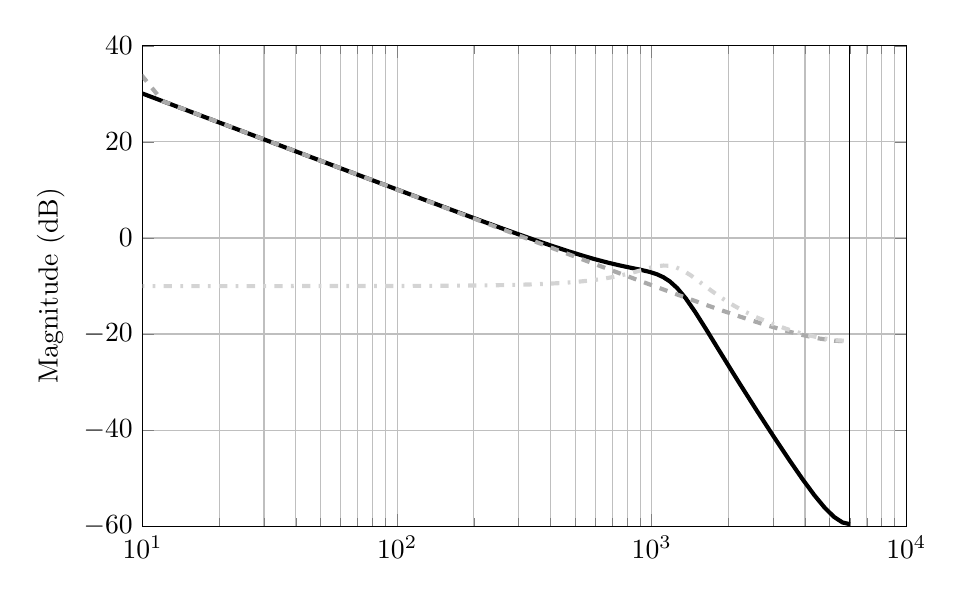
\begin{tikzpicture}

\begin{axis}[%
width=0.8\textwidth,
height=0.503129594988472\textwidth,
scale only axis,
xmode=log,
xmin=10,
xmax=10000,
xminorticks=true,
xmajorgrids,
xminorgrids,
ymin=-60,
ymax=40,
ylabel={Magnitude (dB)},
ymajorgrids
]
\addplot [color=black,solid,line width=1.5pt,forget plot]
  table[row sep=crcr]{5.63236632903622	35.0432670011346\\
17.8111062161958	25.0440080455449\\
25.281590957036	22.0025736928121\\
29.492925060071	20.6649037869399\\
34.4057709847919	19.3274502775555\\
40.1369845360157	17.9902914366573\\
46.8228870196359	16.6535339328735\\
54.6225077493379	15.3173232057542\\
63.7213666806846	13.981857690972\\
74.3358871454136	12.6474083765336\\
86.718543646219	11.314345780138\\
101.163867156258	9.98317733097734\\
118.015450764032	8.65459946878765\\
137.674122298282	7.32957078664084\\
160.607478325024	6.00941564514448\\
187.361006290177	4.69597252710462\\
218.571059356446	3.39180901303621\\
254.979992550901	2.10053715640982\\
297.453820248141	0.827281066415022\\
347.002814985768	-0.420626611236702\\
404.805537570836	-1.63261782664746\\
472.236870051716	-2.793446466222\\
550.90071834113	-3.88148019887221\\
592.991966218768	-4.36754960280358\\
673.420845070559	-5.14260074555582\\
753.190706707444	-5.74825674469143\\
831.184093405816	-6.22768531087122\\
906.486903712286	-6.6389896889942\\
978.390861760009	-7.05344518389974\\
1046.38293643355	-7.54394135034707\\
1110.12624089311	-8.16364066873115\\
1177.75264466741	-9.04897921944483\\
1259.59912227979	-10.454479339098\\
1359.51249342111	-12.5625641538183\\
1482.68028767217	-15.444696629111\\
1636.21279411	-19.0385502541716\\
1830.02988360176	-23.2384654940708\\
2078.24109081575	-27.9822618725317\\
2204.42009291504	-30.1531697099073\\
2571.6259990024	-35.739469744059\\
3000	-41.2026181441611\\
3030.2689591777	-41.5541302659575\\
3469.23953517283	-46.2249361479944\\
3912.38254234155	-50.2261335056264\\
4353.43031613188	-53.562607674867\\
4786.88753737427	-56.2037703800842\\
5208.13303270343	-58.1014936911297\\
5613.4498161518	-59.2218981435703\\
6000	-59.5807325207587\\
};
\addplot [color=black,solid,forget plot]
  table[row sep=crcr]{6000	-70\\
6000	-60\\
6000	0\\
6000	50\\
};
\addplot [color=mycolor1,dashed,line width=1.5pt,forget plot]
  table[row sep=crcr]{5.60903059281346	50\\
12	28.4815921730464\\
120	8.48300670391026\\
132.294888466487	7.63607813246301\\
145.849479286335	6.78921587025409\\
160.79283829234	5.94243420391471\\
177.267255067459	5.09575049893094\\
195.429597815914	4.24918586350606\\
215.45280705089	3.40276595573213\\
237.527542321575	2.55652196508723\\
261.863997659596	1.7104918060259\\
288.693903031372	0.864721569668679\\
318.272730854084	0.0192672896598784\\
350.882128585544	-0.825802909434174\\
386.8326005509	-1.67040619775158\\
426.466464542353	-2.51444185788398\\
470.161111344397	-3.35778741016285\\
518.332598221554	-4.20029389297422\\
571.43961058554	-5.04178011113033\\
629.987829564556	-5.88202562265889\\
694.534747062392	-6.7207621813492\\
765.69497415599	-7.55766328621546\\
844.146093377636	-8.39233140600693\\
930.63511060679	-9.22428234208686\\
1025.98556800602	-10.0529260597625\\
1131.10538572984	-10.8775431473702\\
1246.99550707477	-11.6972558414477\\
1374.75942938889	-12.5109922673178\\
1515.61371149379	-13.3174421617671\\
1670.89955766957	-14.1150018309287\\
1842.09558850499	-14.9017053965228\\
2030.83192021562	-15.6751384133725\\
2238.90568649256	-16.4323285708213\\
2468.2981506793	-17.1696062151881\\
2721.19357121795	-17.8824245172266\\
3000	-18.5651247041516\\
3446.0950649911	-19.4693163438247\\
3958.52373231868	-20.2708986469465\\
4547.14969953119	-20.9313694824216\\
5223.30337977675	-21.3946073163611\\
6000	-21.5754246607914\\
};
\addplot [color=black,solid,forget plot]
  table[row sep=crcr]{6000	-70\\
6000	-60\\
6000	0\\
6000	50\\
};
\addplot [color=white!50!mycolor1,dash pattern=on 1pt off 3pt on 3pt off 3pt,line width=1.5pt,forget plot]
  table[row sep=crcr]{2.43976253839786	-10.0200706466196\\
24.3976253839786	-10.0183640224931\\
27.9933825081012	-10.0178181283264\\
32.1190874895334	-10.0170992317652\\
36.8528448057946	-10.0161524076803\\
42.2842700846515	-10.0149052215475\\
48.5161866339997	-10.0132620953996\\
55.6665720087595	-10.0110968229421\\
63.8707914656017	-10.0082425985883\\
73.2841605874428	-10.0044786880785\\
84.0848855912249	-9.99951253011145\\
96.4774369824858	-9.99295556826778\\
110.696420423992	-9.98429039044111\\
127.011018098561	-9.97282567151018\\
145.730084646319	-9.95763376964494\\
167.207994148533	-9.93746328910899\\
191.851348848317	-9.91061496858548\\
220.126676612259	-9.87476306175203\\
252.569262855007	-9.82669470530168\\
289.793284125605	-9.76192490150237\\
332.503435196366	-9.6741228058073\\
381.50826976882	-9.55425578069876\\
437.735507352105	-9.38932956471965\\
502.249596091101	-9.1606177518818\\
576.271864029449	-8.84149392787967\\
584.148608542391	-8.80378865295755\\
655.630773732666	-8.42785598877824\\
726.805735062537	-7.99446347559671\\
796.850886763502	-7.51839106259493\\
865.068095952867	-7.02627345517604\\
930.888485960413	-6.55705123666575\\
993.869735192962	-6.15830144779545\\
1053.68798448736	-5.8767717548219\\
1110.1262408931	-5.74487939059836\\
1169.58747642835	-5.78377710778845\\
1239.9816868155	-6.08111055988105\\
1323.87529688691	-6.74027110747475\\
1424.60492588389	-7.79868894636512\\
1546.56321677058	-9.19332763668435\\
1695.61164870749	-10.7952165055576\\
1879.68643342228	-12.4739270342555\\
2109.7033403787	-14.1364526919648\\
2278.79687353469	-15.1195145634274\\
2614.64923471659	-16.653953369939\\
3000	-17.9568473062002\\
3446.0950649911	-19.0757319077946\\
3958.52373231868	-20.0132418175236\\
4547.14969953119	-20.7574781624663\\
5223.30337977675	-21.2677032186179\\
6000	-21.4646570928586\\
};
\addplot [color=black,solid,forget plot]
  table[row sep=crcr]{6000	-70\\
6000	-60\\
6000	0\\
6000	50\\
};
\end{axis}

\begin{axis}[%
width=0.8\textwidth,
height=0.461611624834875\textwidth,
unbounded coords=jump,
scale only axis,
xmode=log,
xmin=10,
xmax=10000,
xminorticks=true,
xmajorgrids,
xminorgrids,
ymin=0,
ymax=1,
ytick={  0, 0.2, 0.4, 0.6, 0.8,   1},
ylabel={Phase (deg)},
ymajorgrids,
hide axis
]
\addplot [color=black,solid,line width=1.5pt,forget plot]
  table[row sep=crcr]{1.59154943091895e-21	-5.11977400923008e-09\\
3.56222124323915e-19	-1.14591557753943e-06\\
3.56222124323915e-16	-0.00114591559009614\\
3.10862860767066e-14	-0.1\\
nan	nan\\
3.10856209313889e-14	-0.1\\
nan	nan\\
3.10856209313889e-14	-0.1\\
nan	nan\\
3.09808311333898e-14	-0.1\\
nan	nan\\
3.09808311333898e-14	-0.1\\
nan	nan\\
3.09155825551187e-14	-0.1\\
nan	nan\\
3.09155825551187e-14	-0.1\\
nan	nan\\
3.08108055605266e-14	-0.1\\
nan	nan\\
3.08108055605266e-14	-0.1\\
nan	nan\\
3.06428505472477e-14	-0.1\\
nan	nan\\
3.06428505472477e-14	-0.1\\
nan	nan\\
3.03740259858303e-14	-0.1\\
nan	nan\\
3.03740259858303e-14	-0.1\\
nan	nan\\
2.99443031509304e-14	-0.1\\
nan	nan\\
2.99443031509304e-14	-0.1\\
nan	nan\\
2.92581401280732e-14	-0.1\\
nan	nan\\
2.92581401280731e-14	-0.1\\
nan	nan\\
2.81635658712049e-14	-0.1\\
nan	nan\\
2.81635658712049e-14	-0.1\\
nan	nan\\
2.64190008043484e-14	-0.100000000000001\\
nan	nan\\
2.64190008043482e-14	-0.0999999999999996\\
nan	nan\\
2.36406684259929e-14	-0.0999999999999988\\
nan	nan\\
2.36406684259929e-14	-0.0999999999999988\\
nan	nan\\
1.92193335012736e-14	-0.0999999999999996\\
nan	nan\\
1.92193335012736e-14	-0.0999999999999996\\
nan	nan\\
1.21886576220422e-14	-0.0999999999999996\\
nan	nan\\
1.21886576220422e-14	-0.0999999999999996\\
nan	nan\\
1.01743217677173e-15	-0.0999999999999996\\
nan	nan\\
1.01743217677173e-15	-0.0999999999999996\\
nan	nan\\
-1.67175519155525e-14	-0.0999999999999996\\
nan	nan\\
-1.67175519155525e-14	-0.0999999999999996\\
nan	nan\\
-4.48449625321773e-14	-0.0999999999999996\\
nan	nan\\
-4.48449625321773e-14	-0.0999999999999996\\
nan	nan\\
-8.94015230992533e-14	-0.100000000000001\\
nan	nan\\
-8.94015230992529e-14	-0.100000000000001\\
nan	nan\\
-1.59879796203936e-13	-0.0999999999999996\\
nan	nan\\
-1.59879796203936e-13	-0.0999999999999996\\
nan	nan\\
-2.71154498879822e-13	-0.0999999999999996\\
nan	nan\\
-2.71154498879822e-13	-0.100000000000001\\
nan	nan\\
-4.46429652598556e-13	-0.100000000000001\\
nan	nan\\
-4.46429652598556e-13	-0.100000000000001\\
nan	nan\\
-7.21696783958457e-13	-0.100000000000001\\
nan	nan\\
-7.21696783958456e-13	-0.100000000000001\\
nan	nan\\
-1.15238614542282e-12	-0.0999999999999979\\
nan	nan\\
-1.15238614542282e-12	-0.0999999999999979\\
nan	nan\\
-1.82312893367793e-12	-0.100000000000001\\
nan	nan\\
-1.82312893367793e-12	-0.0999999999999979\\
nan	nan\\
-2.86182538037997e-12	-0.0999999999999979\\
nan	nan\\
-2.86182538037997e-12	-0.100000000000001\\
nan	nan\\
-4.45953226457143e-12	-0.100000000000009\\
nan	nan\\
-4.45953226457143e-12	-0.100000000000009\\
nan	nan\\
-6.89806782546893e-12	-0.100000000000001\\
nan	nan\\
-6.89806782546893e-12	-0.100000000000001\\
nan	nan\\
-1.0587754414177e-11	-0.100000000000001\\
nan	nan\\
-1.0587754414177e-11	-0.100000000000001\\
nan	nan\\
-1.61185137879053e-11	-0.100000000000001\\
nan	nan\\
-1.61185137879053e-11	-0.100000000000001\\
nan	nan\\
-2.43287748703354e-11	-0.0999999999999943\\
nan	nan\\
-2.43287748703354e-11	-0.0999999999999943\\
nan	nan\\
-3.63985233901724e-11	-0.100000000000001\\
nan	nan\\
-3.63985233901724e-11	-0.100000000000001\\
nan	nan\\
-5.39754531177066e-11	-0.100000000000001\\
nan	nan\\
-5.39754531177066e-11	-0.100000000000001\\
nan	nan\\
-7.93466972062014e-11	-0.100000000000009\\
nan	nan\\
-7.93466972062014e-11	-0.100000000000009\\
nan	nan\\
-1.15673237998856e-10	-0.0999999999999943\\
nan	nan\\
-1.15673237998856e-10	-0.0999999999999943\\
nan	nan\\
-1.67310207039544e-10	-0.0999999999999801\\
nan	nan\\
-1.67310207039544e-10	-0.0999999999999801\\
nan	nan\\
-2.40244512331172e-10	-0.0999999999999943\\
nan	nan\\
-2.40244512331172e-10	-0.0999999999999943\\
nan	nan\\
-3.42692424227065e-10	-0.100000000000009\\
nan	nan\\
-3.42692424227065e-10	-0.100000000000009\\
nan	nan\\
-4.85915044094775e-10	-0.0999999999999943\\
nan	nan\\
-4.85915044094775e-10	-0.0999999999999943\\
nan	nan\\
-6.85330462368343e-10	-0.0999999999999943\\
nan	nan\\
-6.85330462368343e-10	-0.0999999999999943\\
nan	nan\\
-9.62029887426046e-10	-0.0999999999999943\\
nan	nan\\
-9.62029887426046e-10	-0.0999999999999943\\
nan	nan\\
-1.34484381309185e-09	-0.0999999999999943\\
nan	nan\\
-1.34484381309185e-09	-0.0999999999999943\\
nan	nan\\
-1.87315709601406e-09	-0.0999999999999943\\
nan	nan\\
-1.87315709601406e-09	-0.0999999999999943\\
nan	nan\\
-2.60074368511992e-09	-0.0999999999999943\\
nan	nan\\
-2.60074368511992e-09	-0.0999999999999943\\
nan	nan\\
-3.60098956281284e-09	-0.0999999999999943\\
nan	nan\\
-3.60098956281284e-09	-0.0999999999999943\\
nan	nan\\
-4.97400558683425e-09	-0.100000000000009\\
nan	nan\\
-4.97400558683425e-09	-0.100000000000009\\
nan	nan\\
-6.85631310982707e-09	-0.100000000000009\\
nan	nan\\
-6.85631310982707e-09	-0.100000000000009\\
nan	nan\\
-9.43403184896511e-09	-0.0999999999999801\\
nan	nan\\
-9.43403184896511e-09	-0.0999999999999801\\
nan	nan\\
-1.29608350903953e-08	-0.0999999999999943\\
nan	nan\\
-1.29608350903953e-08	-0.0999999999999943\\
nan	nan\\
-2.01918978031513e-08	-0.0999999999999943\\
nan	nan\\
-2.01918978031513e-08	-0.0999999999999943\\
nan	nan\\
-8.60718192359483e-08	-0.0999999999999943\\
nan	nan\\
-8.60718192359483e-08	-0.0999999999999943\\
nan	nan\\
-8.76375163570821e-07	-0.0999999999999801\\
nan	nan\\
-8.76375163570821e-07	-0.0999999999999801\\
nan	nan\\
-8.81406812818038e-06	-0.0999999999999943\\
nan	nan\\
-8.81406812818038e-06	-0.0999999999999943\\
nan	nan\\
-8.83005968778475e-05	-0.0999999999999943\\
nan	nan\\
-8.83005968778475e-05	-0.0999999999999943\\
nan	nan\\
-0.000883511593577896	-0.0999999999999943\\
nan	nan\\
-0.000883511593577896	-0.0999999999999943\\
nan	nan\\
-0.00883662727153813	-0.0999999999999801\\
nan	nan\\
-0.00883662727153813	-0.0999999999999801\\
nan	nan\\
-0.0883622132733536	-0.0999999999999943\\
nan	nan\\
-0.0883622132733536	-0.0999999999999943\\
nan	nan\\
-0.882726366218875	-0.0999999999999943\\
nan	nan\\
-0.882726366218875	-0.0999999999999943\\
nan	nan\\
-8.73715870106724	-0.0999999999999943\\
nan	nan\\
-8.73715870106724	-0.0999999999999943\\
nan	nan\\
-80.8728216648257	-0.0999999999999943\\
nan	nan\\
-80.8728216648258	-0.0999999999999943\\
nan	nan\\
-442.482493968811	-0.0999999999999943\\
nan	nan\\
-442.482493968811	-0.0999999999999943\\
nan	nan\\
-802.201991104795	-0.0999999999999943\\
nan	nan\\
-802.201991104795	-0.0999999999999943\\
nan	nan\\
-874.582431754012	-0.0999999999999943\\
nan	nan\\
-874.582431754012	-0.0999999999999943\\
nan	nan\\
-882.542252894293	-0.0999999999999943\\
nan	nan\\
-882.542252894293	-0.0999999999999943\\
nan	nan\\
-883.326795653021	-0.0999999999999943\\
nan	nan\\
-883.326795653021	-0.0999999999999943\\
nan	nan\\
-883.405634911789	-0.0999999999999943\\
nan	nan\\
-883.405634911789	-0.0999999999999943\\
nan	nan\\
-883.41352630396	-0.0999999999999943\\
nan	nan\\
-883.41352630396	-0.0999999999999943\\
nan	nan\\
-883.414275341573	-0.100000000000009\\
nan	nan\\
-883.414275341573	-0.100000000000009\\
nan	nan\\
-883.414000966472	-0.0999999999999943\\
nan	nan\\
-883.414000966472	-0.0999999999999943\\
nan	nan\\
-883.410474170725	-0.100000000000009\\
nan	nan\\
-883.410474170725	-0.100000000000009\\
nan	nan\\
-883.37496197557	-0.0999999999999943\\
nan	nan\\
-883.37496197557	-0.0999999999999943\\
nan	nan\\
-883.289674184647	-0.0999999999999943\\
nan	nan\\
-883.289674184647	-0.0999999999999943\\
nan	nan\\
-883.213449130125	-0.0999999999999943\\
nan	nan\\
-883.213449130125	-0.0999999999999943\\
nan	nan\\
-883.139900195011	-0.0999999999999943\\
nan	nan\\
-883.139900195011	-0.0999999999999943\\
nan	nan\\
-883.039174771702	-0.0999999999999801\\
nan	nan\\
-883.039174771702	-0.0999999999999801\\
nan	nan\\
-882.901066442308	-0.0999999999999943\\
nan	nan\\
-882.901066442308	-0.0999999999999943\\
nan	nan\\
-882.711427565292	-0.0999999999999943\\
nan	nan\\
-882.711427565292	-0.0999999999999943\\
nan	nan\\
-882.450574375255	-0.0999999999999943\\
nan	nan\\
-882.450574375255	-0.0999999999999943\\
nan	nan\\
-882.090996023911	-0.0999999999999943\\
nan	nan\\
-882.090996023911	-0.0999999999999943\\
nan	nan\\
-881.594028089773	-0.0999999999999943\\
nan	nan\\
-881.594028089773	-0.0999999999999943\\
nan	nan\\
-880.904960458522	-0.0999999999999943\\
nan	nan\\
-880.904960458522	-0.0999999999999943\\
nan	nan\\
-879.945734673906	-0.0999999999999943\\
nan	nan\\
-879.945734673906	-0.0999999999999943\\
nan	nan\\
-878.603855237	-0.100000000000009\\
nan	nan\\
-878.603855237	-0.100000000000009\\
nan	nan\\
-876.71522689873	-0.0999999999999943\\
nan	nan\\
-876.71522689873	-0.0999999999999943\\
nan	nan\\
-874.037033251899	-0.0999999999999943\\
nan	nan\\
-874.037033251898	-0.0999999999999943\\
nan	nan\\
-870.203937760377	-0.0999999999999801\\
nan	nan\\
-870.203937760377	-0.0999999999999801\\
nan	nan\\
-864.655814427538	-0.0999999999999943\\
nan	nan\\
-864.655814427538	-0.0999999999999943\\
nan	nan\\
-856.51613892985	-0.0999999999999801\\
nan	nan\\
-856.51613892985	-0.0999999999999801\\
nan	nan\\
-844.384230420717	-0.100000000000009\\
nan	nan\\
-844.384230420717	-0.100000000000009\\
nan	nan\\
-825.978083479946	-0.100000000000009\\
nan	nan\\
-825.978083479946	-0.0999999999999943\\
nan	nan\\
-797.527378578749	-0.0999999999999943\\
nan	nan\\
-797.527378578749	-0.0999999999999943\\
nan	nan\\
-752.79346323725	-0.0999999999999943\\
nan	nan\\
-752.79346323725	-0.100000000000023\\
nan	nan\\
-705.115489159622	-0.0999999999999943\\
nan	nan\\
-705.115489159622	-0.0999999999999943\\
nan	nan\\
-644.62750498311	-0.100000000000023\\
nan	nan\\
-644.62750498311	-0.100000000000023\\
nan	nan\\
-547.54313133572	-0.0999999999999943\\
nan	nan\\
-547.54313133572	-0.0999999999999943\\
nan	nan\\
-433.081279576356	-0.0999999999999943\\
nan	nan\\
-433.081279576356	-0.0999999999999659\\
nan	nan\\
-309.750056918655	-0.0999999999999659\\
nan	nan\\
-309.750056918655	-0.0999999999999659\\
nan	nan\\
-190.48270882012	-0.100000000000023\\
nan	nan\\
-190.48270882012	-0.100000000000023\\
nan	nan\\
-89.9295838710348	-0.0999999999999943\\
nan	nan\\
-89.9295838710348	-0.0999999999999659\\
nan	nan\\
-20.7163265331617	-0.100000000000023\\
nan	nan\\
-20.7163265331617	-0.100000000000023\\
nan	nan\\
9.6804967223477	-0.0999999999999659\\
nan	nan\\
9.6804967223477	-0.0999999999999659\\
nan	nan\\
-16.2983043873846	-0.0999999999999943\\
nan	nan\\
-16.2983043873846	-0.100000000000023\\
nan	nan\\
-143.786719786582	-0.100000000000023\\
nan	nan\\
-143.786719786582	-0.100000000000023\\
nan	nan\\
-435.91153223374	-0.100000000000023\\
nan	nan\\
-435.91153223374	-0.100000000000023\\
nan	nan\\
-950.046778058532	-0.100000000000023\\
nan	nan\\
-950.046778058532	-0.100000000000023\\
};
\addplot [color=black,solid,forget plot]
  table[row sep=crcr]{6000	-0.1\\
6000	0\\
6000	1\\
6000	1.10000000000002\\
};
\addplot [color=black,solid,forget plot]
  table[row sep=crcr]{6000	-0.1\\
6000	0\\
6000	1\\
6000	1.10000000000002\\
};
\addplot [color=white!50!mycolor1,dash pattern=on 1pt off 3pt on 3pt off 3pt,line width=1.5pt,forget plot]
  table[row sep=crcr]{1983.19530484192	1.1\\
nan	nan\\
2006.3634915977	-0.0999999999999996\\
};
\addplot [color=black,solid,forget plot]
  table[row sep=crcr]{6000	-0.1\\
6000	0\\
6000	1\\
6000	1.10000000000002\\
};
\end{axis}
\end{tikzpicture}%}}\\
  %   \subfloat[Margem de fase para $G(z)$, $G_o(z)$ e $\Delta(z)$.]{\label{fig:phase_g_go_delta_ic}
  %     {\def\svgwidth{0.8\textwidth}% This file was created by matlab2tikz v0.4.7 running on MATLAB 8.3.
% Copyright (c) 2008--2014, Nico Schlömer <nico.schloemer@gmail.com>
% All rights reserved.
% Minimal pgfplots version: 1.3
% 
% The latest updates can be retrieved from
%   http://www.mathworks.com/matlabcentral/fileexchange/22022-matlab2tikz
% where you can also make suggestions and rate matlab2tikz.
% 
%
% defining custom colors
\definecolor{mycolor1}{rgb}{0.33333,0.33333,0.33333}%
%
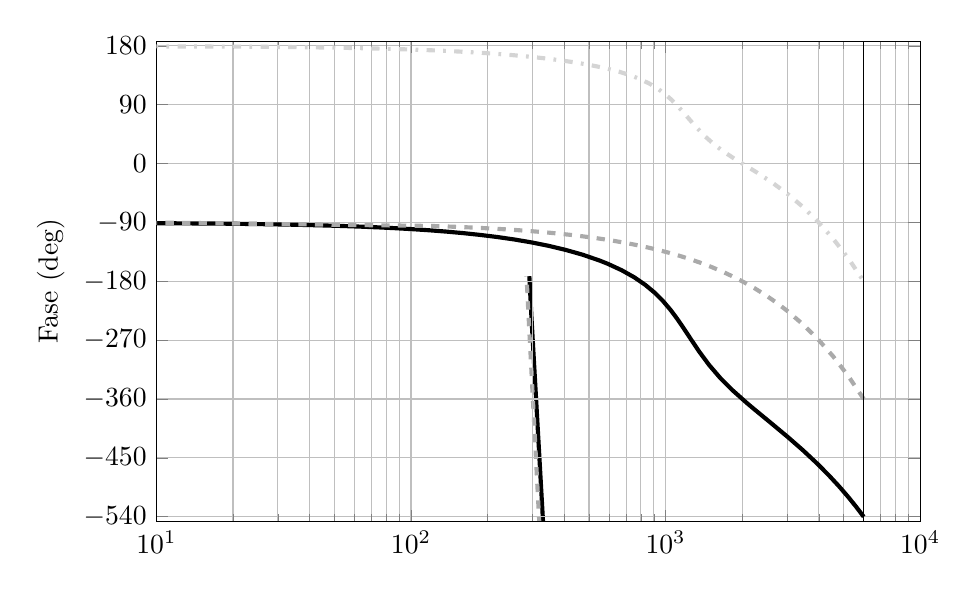
\begin{tikzpicture}

\begin{axis}[%
width=0.8\textwidth,
height=0.256994536928635\textwidth,
unbounded coords=jump,
scale only axis,
xmode=log,
xmin=10,
xmax=10000,
xtick={10,100,1000,10000},
xticklabels={\empty},
xminorticks=true,
xmajorgrids,
xminorgrids,
ymin=0,
ymax=1,
ylabel={Magnitude (dB)},
ymajorgrids,
hide axis
]
\addplot [color=black,solid,line width=1.5pt,forget plot]
  table[row sep=crcr]{288.356344032723	1.1\\
297.453820248141	0.827281066415022\\
334.272124601039	-0.1\\
};
\addplot [color=black,solid,forget plot]
  table[row sep=crcr]{6000	-0.100000000000001\\
6000	0\\
6000	1.10000000000001\\
};
\addplot [color=mycolor1,dashed,line width=1.5pt,forget plot]
  table[row sep=crcr]{281.230294417054	1.1\\
288.693903031372	0.864721569668679\\
318.272730854084	0.0192672896598784\\
322.874992878046	-0.1\\
};
\addplot [color=black,solid,forget plot]
  table[row sep=crcr]{6000	-0.100000000000001\\
6000	0\\
6000	1.10000000000001\\
};
\addplot [color=white!50!mycolor1,dash pattern=on 1pt off 3pt on 3pt off 3pt,line width=1.5pt,forget plot]
  table[row sep=crcr]{10642.3251277333	-0.0999999999999996\\
nan	nan\\
10642.3251277333	-0.0999999999999996\\
nan	nan\\
9196.75220595149	-0.0999999999999996\\
nan	nan\\
9196.75220595149	-0.0999999999999996\\
nan	nan\\
7929.19026058854	-0.0999999999999996\\
nan	nan\\
7929.19026058854	-0.0999999999999996\\
nan	nan\\
6817.36895929562	-0.0999999999999996\\
nan	nan\\
6817.36895929562	-0.0999999999999996\\
nan	nan\\
5842.62310530002	-0.0999999999999979\\
nan	nan\\
5842.62310530002	-0.0999999999999979\\
nan	nan\\
4989.70698106789	-0.0999999999999996\\
nan	nan\\
4989.70698106789	-0.0999999999999996\\
nan	nan\\
4246.66000870045	-0.0999999999999996\\
nan	nan\\
4246.66000870045	-0.0999999999999996\\
nan	nan\\
3604.68708824013	-0.0999999999999996\\
nan	nan\\
3604.68708824013	-0.0999999999999996\\
nan	nan\\
3058.03143535033	-0.0999999999999996\\
nan	nan\\
3058.03143535033	-0.0999999999999996\\
nan	nan\\
2603.90238561226	-0.0999999999999996\\
nan	nan\\
2603.90238561226	-0.0999999999999996\\
nan	nan\\
2402.39604621784	-0.0999999999999979\\
nan	nan\\
2402.39604621784	-0.0999999999999979\\
nan	nan\\
2239.14089188171	-0.0999999999999996\\
nan	nan\\
2239.14089188171	-0.0999999999999996\\
nan	nan\\
2023.29359654141	-0.0999999999999979\\
nan	nan\\
2023.29359654141	-0.0999999999999988\\
nan	nan\\
1888.32838717183	-0.0999999999999996\\
nan	nan\\
1888.32838717183	-0.0999999999999996\\
nan	nan\\
1825.18624265497	-0.0999999999999996\\
nan	nan\\
1825.18624265497	-0.0999999999999996\\
nan	nan\\
1836.65469636147	-0.0999999999999988\\
nan	nan\\
1836.65469636147	-0.0999999999999988\\
nan	nan\\
1950.75900274723	-0.100000000000001\\
nan	nan\\
1950.75900274723	-0.0999999999999996\\
nan	nan\\
2281.11223695961	-0.0999999999999996\\
nan	nan\\
2281.11223695961	-0.0999999999999996\\
nan	nan\\
3525.63491951592	-0.100000000000001\\
nan	nan\\
3525.63491951592	-0.100000000000001\\
nan	nan\\
-176.056610045847	-0.0999999999999988\\
nan	nan\\
-176.056610045847	-0.0999999999999988\\
nan	nan\\
478.745355338468	-0.100000000000001\\
nan	nan\\
478.745355338468	-0.100000000000001\\
nan	nan\\
691.920675074695	-0.0999999999999996\\
nan	nan\\
691.920675074695	-0.0999999999999996\\
nan	nan\\
751.37037955703	-0.0999999999999996\\
nan	nan\\
751.37037955703	-0.0999999999999996\\
nan	nan\\
700.470674602088	-0.0999999999999996\\
nan	nan\\
700.470674602088	-0.0999999999999996\\
nan	nan\\
522.854558022086	-0.0999999999999996\\
nan	nan\\
522.854558022086	-0.0999999999999996\\
nan	nan\\
167.705382107049	-0.0999999999999996\\
nan	nan\\
167.705382107049	-0.0999999999999996\\
nan	nan\\
-304.664918182719	-0.100000000000001\\
nan	nan\\
-304.664918182719	-0.100000000000001\\
};
\addplot [color=black,solid,forget plot]
  table[row sep=crcr]{6000	-0.100000000000001\\
6000	0\\
6000	1.10000000000001\\
};
\end{axis}

\begin{axis}[%
width=0.8\textwidth,
height=0.503129594988472\textwidth,
scale only axis,
xmode=log,
xmin=10,
xmax=10000,
xminorticks=true,
xmajorgrids,
xminorgrids,
ymin=-547.2,
ymax=187.2,
ytick={-540, -450, -360, -270, -180,  -90,    0,   90,  180},
ylabel={Fase (deg)},
ymajorgrids
]
\addplot [color=black,solid,line width=1.5pt,forget plot]
  table[row sep=crcr]{5.63236632903622	-90.5731753048053\\
17.8111062161958	-91.8125905871337\\
25.281590957036	-92.5729245291588\\
29.492925060071	-93.0015833148355\\
34.4057709847919	-93.5016871379265\\
40.1369845360157	-94.0851608575301\\
46.8228870196359	-94.7659297811241\\
54.6225077493379	-95.5602612401483\\
63.7213666806846	-96.4871680813995\\
74.3358871454136	-97.568887467274\\
86.718543646219	-98.8314525714594\\
101.163867156258	-100.305380981591\\
118.015450764032	-102.026513210253\\
137.674122298282	-104.037050063961\\
160.607478325024	-106.386863156314\\
187.361006290177	-109.135197037143\\
218.571059356446	-112.352960924613\\
254.979992550901	-116.125956826115\\
297.453820248141	-120.559680308422\\
347.002814985768	-125.786915521159\\
404.805537570836	-131.980576406809\\
472.236870051716	-139.376933003231\\
550.90071834113	-148.320433609102\\
592.991966218768	-153.287553439495\\
673.420845070559	-163.242716123888\\
753.190706707444	-173.901402329007\\
831.184093405816	-185.328259017269\\
906.486903712286	-197.55351184909\\
978.390861760009	-210.496157543346\\
1046.38293643355	-223.886588582288\\
1110.12624089311	-237.254507711299\\
1177.75264466741	-251.828516998296\\
1259.59912227979	-269.083302019995\\
1359.51249342111	-288.233437128933\\
1482.68028767217	-307.999664713086\\
1636.21279411	-327.431605073632\\
1830.02988360176	-346.429746015136\\
2078.24109081575	-365.603308855363\\
2204.42009291504	-374.011177658143\\
2571.6259990024	-395.469009740435\\
3000	-417.140139676215\\
3030.2689591777	-418.582590833332\\
3469.23953517283	-438.598874932285\\
3912.38254234155	-457.566887394728\\
4353.43031613188	-475.657122384976\\
4786.88753737427	-492.935432581754\\
5208.13303270343	-509.420022172599\\
5613.4498161518	-525.109959539907\\
6000	-540\\
};
\addplot [color=black,solid,forget plot]
  table[row sep=crcr]{6000	-620.64\\
6000	-1\\
6000	0\\
6000	1\\
6000	260.64\\
};
\addplot [color=mycolor1,dashed,line width=1.5pt,forget plot]
  table[row sep=crcr]{0.12	-90.0054\\
12	-90.54\\
120	-95.4\\
132.294888466487	-95.9532699809919\\
145.849479286335	-96.5632265678851\\
160.79283829234	-97.2356777231553\\
177.267255067459	-97.9770264780356\\
195.429597815914	-98.7943319017161\\
215.45280705089	-99.69537631729\\
237.527542321575	-100.688739404471\\
261.863997659596	-101.783879894682\\
288.693903031372	-102.991225636412\\
318.272730854084	-104.322272888434\\
350.882128585544	-105.789695786349\\
386.8326005509	-107.407467024791\\
426.466464542353	-109.190990904406\\
470.161111344397	-111.157250010498\\
518.332598221554	-113.32496691997\\
571.43961058554	-115.714782476349\\
629.987829564556	-118.349452330405\\
694.534747062392	-121.254063617808\\
765.69497415599	-124.45627383702\\
844.146093377636	-127.986574201994\\
930.63511060679	-131.878579977306\\
1025.98556800602	-136.169350560271\\
1131.10538572984	-140.899742357843\\
1246.99550707477	-146.114797818365\\
1374.75942938889	-151.8641743225\\
1515.61371149379	-158.20261701722\\
1670.89955766957	-165.190480095131\\
1842.09558850499	-172.894301482724\\
2030.83192021562	-181.387436409703\\
2238.90568649256	-190.750755892165\\
2468.2981506793	-201.073416780568\\
2721.19357121795	-212.453710704808\\
3000	-225\\
3446.0950649911	-245.074277924599\\
3958.52373231868	-268.133567954341\\
4547.14969953119	-294.621736478903\\
5223.30337977675	-325.048652089954\\
6000	-360\\
};
\addplot [color=black,solid,forget plot]
  table[row sep=crcr]{6000	-620.64\\
6000	-1\\
6000	0\\
6000	1\\
6000	260.64\\
};
\addplot [color=white!50!mycolor1,dash pattern=on 1pt off 3pt on 3pt off 3pt,line width=1.5pt,forget plot]
  table[row sep=crcr]{2.43976253839786	179.861551343359\\
24.3976253839786	178.615487233333\\
27.9933825081012	178.411426085402\\
32.1190874895334	178.177285131634\\
36.8528448057946	177.908628578641\\
42.2842700846515	177.600365512722\\
48.5161866339997	177.246652604704\\
55.6665720087595	176.840782051767\\
63.8707914656017	176.375052320196\\
73.2841605874428	175.84061871738\\
84.0848855912249	175.227320073107\\
96.4774369824858	174.523476706041\\
110.696420423992	173.715653125963\\
127.011018098561	172.788376073918\\
145.730084646319	171.723793565268\\
167.207994148533	170.50125169025\\
191.851348848317	169.096749317818\\
220.126676612259	167.482199088413\\
252.569262855007	165.624361076198\\
289.793284125605	163.483192286247\\
332.503435196366	161.009106300318\\
381.50826976882	158.138126808907\\
437.735507352105	154.782854789887\\
502.249596091101	150.814920952702\\
576.271864029449	146.02981591784\\
584.148608542391	145.501458471037\\
655.630773732666	140.485417093067\\
726.805735062537	134.981360209238\\
796.850886763502	128.882502333374\\
865.068095952867	122.091042097891\\
930.888485960413	114.559900121033\\
993.869735192962	106.343816764535\\
1053.68798448736	97.6377607363639\\
1110.1262408931	88.7687185674626\\
1169.58747642835	79.0511620478742\\
1239.9816868155	67.6346440564047\\
1323.87529688691	55.017862441169\\
1424.60492588389	42.0734244222785\\
1546.56321677058	29.5997775207419\\
1695.61164870749	17.8566822612378\\
1879.68643342228	6.46125882499442\\
2109.7033403787	-5.45250426994392\\
2278.79687353469	-13.4668635160034\\
2614.64923471659	-28.6860488213242\\
3000	-45.8151787041203\\
3446.0950649911	-65.6223073229929\\
3958.52373231868	-88.4584838100648\\
4547.14969953119	-114.789752263717\\
5223.30337977675	-145.11661302007\\
6000	-180\\
};
\addplot [color=black,solid,forget plot]
  table[row sep=crcr]{6000	-620.64\\
6000	-1\\
6000	0\\
6000	1\\
6000	260.64\\
};
\end{axis}
\end{tikzpicture}%}}\\
  %   \subfloat[Diagrama de pólos e zeros para $\Delta(z)$.]{\label{fig:pzmap_delta_ic}
  %     {\def\svgwidth{0.8\textwidth}% This file was created by matlab2tikz v0.4.7 running on MATLAB 8.3.
% Copyright (c) 2008--2014, Nico Schlömer <nico.schloemer@gmail.com>
% All rights reserved.
% Minimal pgfplots version: 1.3
% 
% The latest updates can be retrieved from
%   http://www.mathworks.com/matlabcentral/fileexchange/22022-matlab2tikz
% where you can also make suggestions and rate matlab2tikz.
% 
%
% defining custom colors
\definecolor{mycolor1}{rgb}{0.66667,0.66667,0.66667}%
%
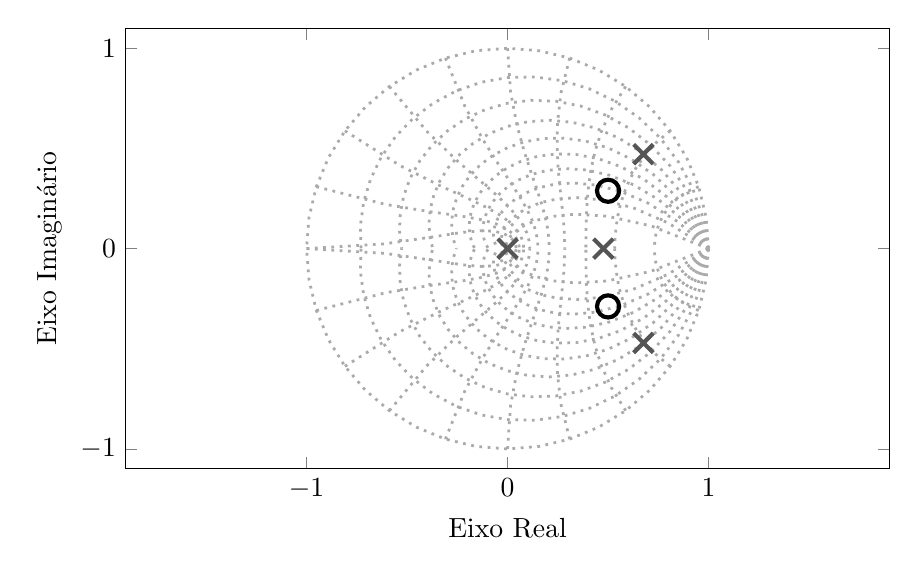
\begin{tikzpicture}

\begin{axis}[%
width=0.8\textwidth,
height=0.461611624834875\textwidth,
scale only axis,
xmin=-1.9,
xmax=1.9,
xtick={-1,  0,  1},
xlabel={Eixo Real},
ymin=-1.1,
ymax=1.1,
ytick={-1,  0,  1},
ylabel={Eixo Imaginário}
]
\addplot [color=mycolor1,dotted,line width=1.0pt,forget plot]
  table[row sep=crcr]{1	0\\
0.987688340595138	0.156434465040231\\
0.951056516295154	0.309016994374947\\
0.891006524188368	0.453990499739547\\
0.809016994374947	0.587785252292473\\
0.707106781186548	0.707106781186547\\
0.587785252292473	0.809016994374947\\
0.453990499739547	0.891006524188368\\
0.309016994374947	0.951056516295154\\
0.156434465040231	0.987688340595138\\
6.12323399573677e-17	1\\
-0.156434465040231	0.987688340595138\\
-0.309016994374947	0.951056516295154\\
-0.453990499739547	0.891006524188368\\
-0.587785252292473	0.809016994374947\\
-0.707106781186547	0.707106781186548\\
-0.809016994374947	0.587785252292473\\
-0.891006524188368	0.453990499739547\\
-0.951056516295154	0.309016994374948\\
-0.987688340595138	0.156434465040231\\
-1	1.22464679914735e-16\\
};
\addplot [color=mycolor1,dotted,line width=1.0pt,forget plot]
  table[row sep=crcr]{1	0\\
0.972218045703082	0.153984211042097\\
0.921496791140463	0.299412457456957\\
0.849791018366557	0.432990150609548\\
0.759508516401756	0.551815237548133\\
0.653437051516106	0.653437051516106\\
0.534664304371591	0.735902282058355\\
0.406492952796512	0.797787339572243\\
0.272353130096494	0.83821674479613\\
0.135714483753824	0.856867527364047\\
5.22899666167123e-17	0.853959960588124\\
-0.131496350792703	0.830235283991667\\
-0.255686250369537	0.786921363444393\\
-0.369756251949576	0.725687504552447\\
-0.47122811850853	0.648589862732789\\
-0.558009078759514	0.558009078759514\\
-0.628431083783263	0.456581908289041\\
-0.681278445058817	0.347128705949459\\
-0.715803538350409	0.232578668243255\\
-0.731730559897045	0.115894735197653\\
-0.729247614287671	8.9307075662324e-17\\
};
\addplot [color=mycolor1,dotted,line width=1.0pt,forget plot]
  table[row sep=crcr]{1	0\\
0.956521682769877	0.151498151383791\\
0.891982039736211	0.289822533396298\\
0.809292583610082	0.412355167436434\\
0.711634858347723	0.517032989000692\\
0.602364630186427	0.602364630186426\\
0.484917701774751	0.667431957639199\\
0.362719588349683	0.711877274647591\\
0.239101059900595	0.735877395777214\\
0.117221283062812	0.740106053489981\\
4.44354699422903e-17	0.725686295399261\\
-0.109940132237539	0.694134676438339\\
-0.210320240583588	0.647299141978847\\
-0.299240493845688	0.587292536894097\\
-0.375203754387119	0.516423664031337\\
-0.437127756959533	0.437127756959533\\
-0.484346224770267	0.351898130574443\\
-0.516599582217932	0.263220634338226\\
-0.534016141209622	0.173512362385299\\
-0.537084820159711	0.0850658786478001\\
-0.526620599330303	6.44924231334916e-17\\
};
\addplot [color=mycolor1,dotted,line width=1.0pt,forget plot]
  table[row sep=crcr]{1	0\\
0.940082788364644	0.148894486293864\\
0.86158608093073	0.279946287694513\\
0.768279786681378	0.391458103646313\\
0.663960650859636	0.482395649771645\\
0.552351927561387	0.552351927561387\\
0.437014383712816	0.601498696728173\\
0.321269860940431	0.630527604183869\\
0.208138182971344	0.640583459188477\\
0.100287778328637	0.633192112325829\\
3.73630739569174e-17	0.610185303761559\\
-0.0908532273476425	0.573624701779294\\
-0.170819110593797	0.525727164509449\\
-0.238861981883349	0.468793035010043\\
-0.294350736089166	0.40513903143051\\
-0.337037028702328	0.337037028702328\\
-0.367025664975262	0.266659754473976\\
-0.384738677688982	0.196034147687371\\
-0.390874612629551	0.127002860400749\\
-0.386364521398959	0.0611941284830315\\
-0.372326104926586	4.55967972637346e-17\\
};
\addplot [color=mycolor1,dotted,line width=1.0pt,forget plot]
  table[row sep=crcr]{1	0\\
0.922246029428501	0.146069421212559\\
0.829201462983264	0.269423887468404\\
0.725373165529273	0.369596088217499\\
0.614985835074999	0.446813363302878\\
0.501902475185001	0.501902475185001\\
0.38956496084428	0.536190168955128\\
0.280953750703967	0.551402782692681\\
0.178565395716864	0.549567778706978\\
0.0844061798404073	0.532919645815306\\
3.08495992433718e-17	0.50381218919366\\
-0.0735915548753502	0.464638791061534\\
-0.135739038566523	0.417761804348184\\
-0.186207014322272	0.365451842507638\\
-0.225110018726605	0.309837359892227\\
-0.252864584784672	0.252864584784672\\
-0.270139142845401	0.196267575756099\\
-0.277803443075876	0.141547924204336\\
-0.27687894570066	0.0899634229303457\\
-0.268491413422519	0.0425248622468694\\
-0.253826721980109	3.10848082611005e-17\\
};
\addplot [color=mycolor1,dotted,line width=1.0pt,forget plot]
  table[row sep=crcr]{1	0\\
0.902056570675584	0.142871725087523\\
0.793293726869509	0.257756756757911\\
0.678769666307395	0.345850419328459\\
0.562876391436159	0.408953636388562\\
0.449318435861499	0.449318435861499\\
0.341115747349381	0.469505547439701\\
0.24062663375655	0.472256359314945\\
0.149586755320764	0.460380694230177\\
0.069160331541479	0.436661148025441\\
2.47240337905553e-17	0.403774113610049\\
-0.057687904157153	0.364227092250654\\
-0.104075505986926	0.320311471399148\\
-0.139645446506012	0.274069620358657\\
-0.165124892040398	0.227274916024158\\
-0.18142315316863	0.18142315316863\\
-0.189574186252466	0.137733708524426\\
-0.190684892879101	0.0971588057560207\\
-0.185889806735969	0.0603992595374446\\
-0.176312467991919	0.0279251515651378\\
-0.16303353482158	1.99658496572927e-17\\
};
\addplot [color=mycolor1,dotted,line width=1.0pt,forget plot]
  table[row sep=crcr]{1	0\\
0.877921760602431	0.139049146701748\\
0.751411952540787	0.244148543365328\\
0.625732257688895	0.318826509862098\\
0.505011411193747	0.36691226736026\\
0.392341669548685	0.392341669548685\\
0.289890514921595	0.399000063654162\\
0.199020572856858	0.390599867100522\\
0.120411913496453	0.370589763847805\\
0.0541820486548744	0.34209199176291\\
1.88512313530119e-17	0.307863971328499\\
-0.042808222513439	0.270280479734772\\
-0.075164540154518	0.231332667812908\\
-0.0981551954909503	0.192640417840451\\
-0.112959067758674	0.155474818616317\\
-0.120787864504912	0.120787864504912\\
-0.122837744156894	0.0892468451742257\\
-0.120251626285951	0.0612712639357851\\
-0.114091236431876	0.0370704898842818\\
-0.105317799143806	0.0166807006736036\\
-0.0947802248421549	1.16072298975411e-17\\
};
\addplot [color=mycolor1,dotted,line width=1.0pt,forget plot]
  table[row sep=crcr]{1	0\\
0.84674396664984	0.134111069256013\\
0.698989566160914	0.227115477506975\\
0.561406498364893	0.286050898428465\\
0.437004973478602	0.317502698182059\\
0.327450698344114	0.327450698344114\\
0.233352139914598	0.321181666481713\\
0.154515499860225	0.303253743289057\\
0.0901653834921457	0.27750051639687\\
0.0391311034995635	0.247064063991275\\
1.31311479217367e-17	0.214447919692096\\
-0.0287598398096346	0.181582482159892\\
-0.0487044416812479	0.149896858349689\\
-0.0613430200940395	0.120392455675976\\
-0.06808779312177	0.0937148074575858\\
-0.0702211210616195	0.0702211210616195\\
-0.068876740220244	0.0500418809603846\\
-0.0650321343871793	0.0331355275052096\\
-0.0595094084547913	0.0193357789181307\\
-0.0529823745536039	0.00839158374073751\\
-0.0459879102602678	5.63189470997126e-18\\
};
\addplot [color=mycolor1,dotted,line width=1.0pt,forget plot]
  table[row sep=crcr]{1	0\\
0.801053465278425	0.126874404768154\\
0.625589539649299	0.203266363189334\\
0.475341369738971	0.242198525079547\\
0.350045057714404	0.254322621147605\\
0.24813777530853	0.24813777530853\\
0.167289292234614	0.230253957320141\\
0.104794333468008	0.205670459781722\\
0.0578515468028918	0.178048753195384\\
0.0237523524567972	0.149966451301199\\
7.54043881219821e-18	0.123144711070133\\
-0.0156239119173694	0.0986454975334405\\
-0.0250311775652273	0.0770380431086105\\
-0.0298254673925332	0.0585357756361869\\
-0.0313184856998208	0.0431061974937683\\
-0.0305568546459545	0.0305568546459545\\
-0.0283545570469435	0.0206007915573586\\
-0.0253272293454815	0.012904867916705\\
-0.021925762268643	0.00712411201600239\\
-0.0184675753156993	0.00292497658052826\\
-0.0151646198645466	1.85713031774033e-18\\
};
\addplot [color=mycolor1,dotted,line width=1.0pt,forget plot]
  table[row sep=crcr]{1	0\\
0.714110955679367	0.113104064044896\\
0.497161927717827	0.161537702532642\\
0.336758208677056	0.171586877647116\\
0.221075553032581	0.160620791180475\\
0.139705610200823	0.139705610200823\\
0.0839640345306934	0.115566579097864\\
0.0468885871776745	0.0920240337831981\\
0.0230753615892199	0.0710186604775083\\
0.00844586939409394	0.0533251206797082\\
2.39022368106624e-18	0.0390353150431684\\
-0.00441505277265522	0.0278755461307222\\
-0.00630567510971132	0.0194068724759343\\
-0.00669794782622876	0.0131454627690819\\
-0.0062698831862128	0.00862975386096949\\
-0.0054534525074872	0.0054534525074872\\
-0.00451117782354635	0.00327756254020109\\
-0.00359218715027031	0.00183031077240959\\
-0.00277223578568335	0.000900754009370227\\
-0.00208156288544739	0.000329687172611911\\
-0.00152375582051941	1.86606268828125e-19\\
};
\addplot [color=mycolor1,dotted,line width=1.0pt,forget plot]
  table[row sep=crcr]{1	-0\\
0.987688340595138	-0.156434465040231\\
0.951056516295154	-0.309016994374947\\
0.891006524188368	-0.453990499739547\\
0.809016994374947	-0.587785252292473\\
0.707106781186548	-0.707106781186547\\
0.587785252292473	-0.809016994374947\\
0.453990499739547	-0.891006524188368\\
0.309016994374947	-0.951056516295154\\
0.156434465040231	-0.987688340595138\\
6.12323399573677e-17	-1\\
-0.156434465040231	-0.987688340595138\\
-0.309016994374947	-0.951056516295154\\
-0.453990499739547	-0.891006524188368\\
-0.587785252292473	-0.809016994374947\\
-0.707106781186547	-0.707106781186548\\
-0.809016994374947	-0.587785252292473\\
-0.891006524188368	-0.453990499739547\\
-0.951056516295154	-0.309016994374948\\
-0.987688340595138	-0.156434465040231\\
-1	-1.22464679914735e-16\\
};
\addplot [color=mycolor1,dotted,line width=1.0pt,forget plot]
  table[row sep=crcr]{1	-0\\
0.972218045703082	-0.153984211042097\\
0.921496791140463	-0.299412457456957\\
0.849791018366557	-0.432990150609548\\
0.759508516401756	-0.551815237548133\\
0.653437051516106	-0.653437051516106\\
0.534664304371591	-0.735902282058355\\
0.406492952796512	-0.797787339572243\\
0.272353130096494	-0.83821674479613\\
0.135714483753824	-0.856867527364047\\
5.22899666167123e-17	-0.853959960588124\\
-0.131496350792703	-0.830235283991667\\
-0.255686250369537	-0.786921363444393\\
-0.369756251949576	-0.725687504552447\\
-0.47122811850853	-0.648589862732789\\
-0.558009078759514	-0.558009078759514\\
-0.628431083783263	-0.456581908289041\\
-0.681278445058817	-0.347128705949459\\
-0.715803538350409	-0.232578668243255\\
-0.731730559897045	-0.115894735197653\\
-0.729247614287671	-8.9307075662324e-17\\
};
\addplot [color=mycolor1,dotted,line width=1.0pt,forget plot]
  table[row sep=crcr]{1	-0\\
0.956521682769877	-0.151498151383791\\
0.891982039736211	-0.289822533396298\\
0.809292583610082	-0.412355167436434\\
0.711634858347723	-0.517032989000692\\
0.602364630186427	-0.602364630186426\\
0.484917701774751	-0.667431957639199\\
0.362719588349683	-0.711877274647591\\
0.239101059900595	-0.735877395777214\\
0.117221283062812	-0.740106053489981\\
4.44354699422903e-17	-0.725686295399261\\
-0.109940132237539	-0.694134676438339\\
-0.210320240583588	-0.647299141978847\\
-0.299240493845688	-0.587292536894097\\
-0.375203754387119	-0.516423664031337\\
-0.437127756959533	-0.437127756959533\\
-0.484346224770267	-0.351898130574443\\
-0.516599582217932	-0.263220634338226\\
-0.534016141209622	-0.173512362385299\\
-0.537084820159711	-0.0850658786478001\\
-0.526620599330303	-6.44924231334916e-17\\
};
\addplot [color=mycolor1,dotted,line width=1.0pt,forget plot]
  table[row sep=crcr]{1	-0\\
0.940082788364644	-0.148894486293864\\
0.86158608093073	-0.279946287694513\\
0.768279786681378	-0.391458103646313\\
0.663960650859636	-0.482395649771645\\
0.552351927561387	-0.552351927561387\\
0.437014383712816	-0.601498696728173\\
0.321269860940431	-0.630527604183869\\
0.208138182971344	-0.640583459188477\\
0.100287778328637	-0.633192112325829\\
3.73630739569174e-17	-0.610185303761559\\
-0.0908532273476425	-0.573624701779294\\
-0.170819110593797	-0.525727164509449\\
-0.238861981883349	-0.468793035010043\\
-0.294350736089166	-0.40513903143051\\
-0.337037028702328	-0.337037028702328\\
-0.367025664975262	-0.266659754473976\\
-0.384738677688982	-0.196034147687371\\
-0.390874612629551	-0.127002860400749\\
-0.386364521398959	-0.0611941284830315\\
-0.372326104926586	-4.55967972637346e-17\\
};
\addplot [color=mycolor1,dotted,line width=1.0pt,forget plot]
  table[row sep=crcr]{1	-0\\
0.922246029428501	-0.146069421212559\\
0.829201462983264	-0.269423887468404\\
0.725373165529273	-0.369596088217499\\
0.614985835074999	-0.446813363302878\\
0.501902475185001	-0.501902475185001\\
0.38956496084428	-0.536190168955128\\
0.280953750703967	-0.551402782692681\\
0.178565395716864	-0.549567778706978\\
0.0844061798404073	-0.532919645815306\\
3.08495992433718e-17	-0.50381218919366\\
-0.0735915548753502	-0.464638791061534\\
-0.135739038566523	-0.417761804348184\\
-0.186207014322272	-0.365451842507638\\
-0.225110018726605	-0.309837359892227\\
-0.252864584784672	-0.252864584784672\\
-0.270139142845401	-0.196267575756099\\
-0.277803443075876	-0.141547924204336\\
-0.27687894570066	-0.0899634229303457\\
-0.268491413422519	-0.0425248622468694\\
-0.253826721980109	-3.10848082611005e-17\\
};
\addplot [color=mycolor1,dotted,line width=1.0pt,forget plot]
  table[row sep=crcr]{1	-0\\
0.902056570675584	-0.142871725087523\\
0.793293726869509	-0.257756756757911\\
0.678769666307395	-0.345850419328459\\
0.562876391436159	-0.408953636388562\\
0.449318435861499	-0.449318435861499\\
0.341115747349381	-0.469505547439701\\
0.24062663375655	-0.472256359314945\\
0.149586755320764	-0.460380694230177\\
0.069160331541479	-0.436661148025441\\
2.47240337905553e-17	-0.403774113610049\\
-0.057687904157153	-0.364227092250654\\
-0.104075505986926	-0.320311471399148\\
-0.139645446506012	-0.274069620358657\\
-0.165124892040398	-0.227274916024158\\
-0.18142315316863	-0.18142315316863\\
-0.189574186252466	-0.137733708524426\\
-0.190684892879101	-0.0971588057560207\\
-0.185889806735969	-0.0603992595374446\\
-0.176312467991919	-0.0279251515651378\\
-0.16303353482158	-1.99658496572927e-17\\
};
\addplot [color=mycolor1,dotted,line width=1.0pt,forget plot]
  table[row sep=crcr]{1	-0\\
0.877921760602431	-0.139049146701748\\
0.751411952540787	-0.244148543365328\\
0.625732257688895	-0.318826509862098\\
0.505011411193747	-0.36691226736026\\
0.392341669548685	-0.392341669548685\\
0.289890514921595	-0.399000063654162\\
0.199020572856858	-0.390599867100522\\
0.120411913496453	-0.370589763847805\\
0.0541820486548744	-0.34209199176291\\
1.88512313530119e-17	-0.307863971328499\\
-0.042808222513439	-0.270280479734772\\
-0.075164540154518	-0.231332667812908\\
-0.0981551954909503	-0.192640417840451\\
-0.112959067758674	-0.155474818616317\\
-0.120787864504912	-0.120787864504912\\
-0.122837744156894	-0.0892468451742257\\
-0.120251626285951	-0.0612712639357851\\
-0.114091236431876	-0.0370704898842818\\
-0.105317799143806	-0.0166807006736036\\
-0.0947802248421549	-1.16072298975411e-17\\
};
\addplot [color=mycolor1,dotted,line width=1.0pt,forget plot]
  table[row sep=crcr]{1	-0\\
0.84674396664984	-0.134111069256013\\
0.698989566160914	-0.227115477506975\\
0.561406498364893	-0.286050898428465\\
0.437004973478602	-0.317502698182059\\
0.327450698344114	-0.327450698344114\\
0.233352139914598	-0.321181666481713\\
0.154515499860225	-0.303253743289057\\
0.0901653834921457	-0.27750051639687\\
0.0391311034995635	-0.247064063991275\\
1.31311479217367e-17	-0.214447919692096\\
-0.0287598398096346	-0.181582482159892\\
-0.0487044416812479	-0.149896858349689\\
-0.0613430200940395	-0.120392455675976\\
-0.06808779312177	-0.0937148074575858\\
-0.0702211210616195	-0.0702211210616195\\
-0.068876740220244	-0.0500418809603846\\
-0.0650321343871793	-0.0331355275052096\\
-0.0595094084547913	-0.0193357789181307\\
-0.0529823745536039	-0.00839158374073751\\
-0.0459879102602678	-5.63189470997126e-18\\
};
\addplot [color=mycolor1,dotted,line width=1.0pt,forget plot]
  table[row sep=crcr]{1	-0\\
0.801053465278425	-0.126874404768154\\
0.625589539649299	-0.203266363189334\\
0.475341369738971	-0.242198525079547\\
0.350045057714404	-0.254322621147605\\
0.24813777530853	-0.24813777530853\\
0.167289292234614	-0.230253957320141\\
0.104794333468008	-0.205670459781722\\
0.0578515468028918	-0.178048753195384\\
0.0237523524567972	-0.149966451301199\\
7.54043881219821e-18	-0.123144711070133\\
-0.0156239119173694	-0.0986454975334405\\
-0.0250311775652273	-0.0770380431086105\\
-0.0298254673925332	-0.0585357756361869\\
-0.0313184856998208	-0.0431061974937683\\
-0.0305568546459545	-0.0305568546459545\\
-0.0283545570469435	-0.0206007915573586\\
-0.0253272293454815	-0.012904867916705\\
-0.021925762268643	-0.00712411201600239\\
-0.0184675753156993	-0.00292497658052826\\
-0.0151646198645466	-1.85713031774033e-18\\
};
\addplot [color=mycolor1,dotted,line width=1.0pt,forget plot]
  table[row sep=crcr]{1	-0\\
0.714110955679367	-0.113104064044896\\
0.497161927717827	-0.161537702532642\\
0.336758208677056	-0.171586877647116\\
0.221075553032581	-0.160620791180475\\
0.139705610200823	-0.139705610200823\\
0.0839640345306934	-0.115566579097864\\
0.0468885871776745	-0.0920240337831981\\
0.0230753615892199	-0.0710186604775083\\
0.00844586939409394	-0.0533251206797082\\
2.39022368106624e-18	-0.0390353150431684\\
-0.00441505277265522	-0.0278755461307222\\
-0.00630567510971132	-0.0194068724759343\\
-0.00669794782622876	-0.0131454627690819\\
-0.0062698831862128	-0.00862975386096949\\
-0.0054534525074872	-0.0054534525074872\\
-0.00451117782354635	-0.00327756254020109\\
-0.00359218715027031	-0.00183031077240959\\
-0.00277223578568335	-0.000900754009370227\\
-0.00208156288544739	-0.000329687172611911\\
-0.00152375582051941	-1.86606268828125e-19\\
};
\addplot [color=mycolor1,dotted,line width=1.0pt,forget plot]
  table[row sep=crcr]{1	0\\
1	0\\
};
\addplot [color=mycolor1,dotted,line width=1.0pt,forget plot]
  table[row sep=crcr]{0.951056516295154	0.309016994374947\\
0.906577591518048	0.290693092532446\\
0.867277205719189	0.267124444629623\\
0.833330533437629	0.239553777474139\\
0.804679893747523	0.20903820245934\\
0.781122098933164	0.176433510213537\\
0.762382187756933	0.142402376999381\\
0.748171074803624	0.107437628337747\\
0.738227708485823	0.0718935522249012\\
0.732347931289196	0.0360204899377399\\
0.730402691048646	2.81010850277162e-17\\
};
\addplot [color=mycolor1,dotted,line width=1.0pt,forget plot]
  table[row sep=crcr]{0.809016994374947	0.587785252292473\\
0.737380455396588	0.527071687397996\\
0.6808142826414	0.463341883835339\\
0.637053765657314	0.399254954339046\\
0.603812761314093	0.336417677088311\\
0.579022949915482	0.275632227640288\\
0.560948163233974	0.217130071437151\\
0.54821711318997	0.160763451735608\\
0.539811466724715	0.106147624627789\\
0.535036016768209	0.0527590625798542\\
0.533488091091103	4.10502162512614e-17\\
};
\addplot [color=mycolor1,dotted,line width=1.0pt,forget plot]
  table[row sep=crcr]{0.587785252292473	0.809016994374947\\
0.515276498489902	0.692182785870847\\
0.46668476526979	0.583707991451876\\
0.435233321876477	0.485319980094308\\
0.415551842123536	0.396928474901319\\
0.403656860517901	0.317461475735791\\
0.396737049613855	0.245416450708029\\
0.392888142823216	0.179177710929467\\
0.39087245229983	0.11717008156476\\
0.389932112762627	0.0579102497954412\\
0.389661137375347	4.49747826270753e-17\\
};
\addplot [color=mycolor1,dotted,line width=1.0pt,forget plot]
  table[row sep=crcr]{0.309016994374947	0.951056516295154\\
0.265925372344309	0.777304721760365\\
0.248822386132444	0.630899544522142\\
0.24643298177389	0.508693744238057\\
0.251412997268255	0.406266573115132\\
0.25929445161488	0.31919477108011\\
0.267517373913267	0.243597429511063\\
0.274697115780397	0.1762665508339\\
0.280129101393366	0.114599409879343\\
0.283480020554887	0.0564559973822998\\
0.284609543336029	4.37996030135249e-17\\
};
\addplot [color=mycolor1,dotted,line width=1.0pt,forget plot]
  table[row sep=crcr]{6.12323399573677e-17	1\\
0.0151248701748503	0.781989711398728\\
0.0472692933177679	0.613631335769719\\
0.0835006201485716	0.482943980920436\\
0.117381749765263	0.379469463911326\\
0.146223972383669	0.295078319831894\\
0.169261627793672	0.223809451176491\\
0.186582776182006	0.161390341419992\\
0.198560105942714	0.104739935929793\\
0.205572433929556	0.0515565221197431\\
0.207879576350762	3.99891848849262e-17\\
};
\addplot [color=mycolor1,dotted,line width=1.0pt,forget plot]
  table[row sep=crcr]{-0.309016994374947	0.951056516295154\\
-0.213607139159912	0.713331044437031\\
-0.122920349149865	0.544815253953639\\
-0.0461074386071066	0.422454854218942\\
0.0151311193047769	0.329888717873058\\
0.0621570724668225	0.256291005261778\\
0.0971710522581798	0.194731597161215\\
0.122256440677152	0.140793596164787\\
0.13905244595299	0.0915971142347777\\
0.148693455532156	0.0451621321066958\\
0.151835801980649	3.50498499033503e-17\\
};
\addplot [color=mycolor1,dotted,line width=1.0pt,forget plot]
  table[row sep=crcr]{-0.587785252292473	0.809016994374948\\
-0.401011853057454	0.584595820351374\\
-0.252139489074835	0.439670821081765\\
-0.139623392550337	0.340999317931598\\
-0.0567836371213516	0.268617800427267\\
0.0033339412143336	0.21116115844769\\
0.0463512370945915	0.162297289886265\\
0.0763422025660035	0.118472638203443\\
0.0960671266193367	0.0776165020305757\\
0.1072685824301	0.0384304051397518\\
0.110901278364195	2.98672554719679e-17\\
};
\addplot [color=mycolor1,dotted,line width=1.0pt,forget plot]
  table[row sep=crcr]{-0.809016994374948	0.587785252292473\\
-0.533486326814499	0.413410095118228\\
-0.336121655437603	0.313963860155743\\
-0.198040110920963	0.250717832404618\\
-0.101844033235305	0.204281393673556\\
-0.0346516892466227	0.165530866251108\\
0.0122258376810533	0.130333089269644\\
0.0443886084751889	0.0968398262452624\\
0.065339288702761	0.0642052594194206\\
0.0771736424133687	0.032008294596762\\
0.0810025921579431	2.49315700239574e-17\\
};
\addplot [color=mycolor1,dotted,line width=1.0pt,forget plot]
  table[row sep=crcr]{-0.951056516295154	0.309016994374948\\
-0.60382220830535	0.219707538176049\\
-0.375378071887508	0.182507388795924\\
-0.225093275108467	0.161489568357552\\
-0.124654461172013	0.143091836517116\\
-0.0562723920172722	0.12318609851568\\
-0.00923898083522721	0.101104614081101\\
0.0228060316514889	0.0772217637055013\\
0.0436193292019494	0.0520955750986265\\
0.0553650029180358	0.0262210407420432\\
0.0591645112940776	2.0486346567262e-17\\
};
\addplot [color=mycolor1,dotted,line width=1.0pt,forget plot]
  table[row sep=crcr]{-1	1.22464679914735e-16\\
-0.61127914703566	0.0236549857259488\\
-0.374309030147768	0.0580118391989452\\
-0.226262535142082	0.0806522438077526\\
-0.130218598863194	0.0890855793127953\\
-0.0656897647351535	0.0862950481802363\\
-0.0214411717925588	0.0757647040434823\\
0.00876629006412298	0.0602253159022079\\
0.0284556614934045	0.0415943455493057\\
0.039601950618638	0.0211971994741971\\
0.0432139182637723	1.66258696249815e-17\\
};
\addplot [color=mycolor1,dotted,line width=1.0pt,forget plot]
  table[row sep=crcr]{1	-0\\
1	-0\\
};
\addplot [color=mycolor1,dotted,line width=1.0pt,forget plot]
  table[row sep=crcr]{0.951056516295154	-0.309016994374947\\
0.906577591518048	-0.290693092532446\\
0.867277205719189	-0.267124444629623\\
0.833330533437629	-0.239553777474139\\
0.804679893747523	-0.20903820245934\\
0.781122098933164	-0.176433510213537\\
0.762382187756933	-0.142402376999381\\
0.748171074803624	-0.107437628337747\\
0.738227708485823	-0.0718935522249012\\
0.732347931289196	-0.0360204899377399\\
0.730402691048646	-2.81010850277162e-17\\
};
\addplot [color=mycolor1,dotted,line width=1.0pt,forget plot]
  table[row sep=crcr]{0.809016994374947	-0.587785252292473\\
0.737380455396588	-0.527071687397996\\
0.6808142826414	-0.463341883835339\\
0.637053765657314	-0.399254954339046\\
0.603812761314093	-0.336417677088311\\
0.579022949915482	-0.275632227640288\\
0.560948163233974	-0.217130071437151\\
0.54821711318997	-0.160763451735608\\
0.539811466724715	-0.106147624627789\\
0.535036016768209	-0.0527590625798542\\
0.533488091091103	-4.10502162512614e-17\\
};
\addplot [color=mycolor1,dotted,line width=1.0pt,forget plot]
  table[row sep=crcr]{0.587785252292473	-0.809016994374947\\
0.515276498489902	-0.692182785870847\\
0.46668476526979	-0.583707991451876\\
0.435233321876477	-0.485319980094308\\
0.415551842123536	-0.396928474901319\\
0.403656860517901	-0.317461475735791\\
0.396737049613855	-0.245416450708029\\
0.392888142823216	-0.179177710929467\\
0.39087245229983	-0.11717008156476\\
0.389932112762627	-0.0579102497954412\\
0.389661137375347	-4.49747826270753e-17\\
};
\addplot [color=mycolor1,dotted,line width=1.0pt,forget plot]
  table[row sep=crcr]{0.309016994374947	-0.951056516295154\\
0.265925372344309	-0.777304721760365\\
0.248822386132444	-0.630899544522142\\
0.24643298177389	-0.508693744238057\\
0.251412997268255	-0.406266573115132\\
0.25929445161488	-0.31919477108011\\
0.267517373913267	-0.243597429511063\\
0.274697115780397	-0.1762665508339\\
0.280129101393366	-0.114599409879343\\
0.283480020554887	-0.0564559973822998\\
0.284609543336029	-4.37996030135249e-17\\
};
\addplot [color=mycolor1,dotted,line width=1.0pt,forget plot]
  table[row sep=crcr]{6.12323399573677e-17	-1\\
0.0151248701748503	-0.781989711398728\\
0.0472692933177679	-0.613631335769719\\
0.0835006201485716	-0.482943980920436\\
0.117381749765263	-0.379469463911326\\
0.146223972383669	-0.295078319831894\\
0.169261627793672	-0.223809451176491\\
0.186582776182006	-0.161390341419992\\
0.198560105942714	-0.104739935929793\\
0.205572433929556	-0.0515565221197431\\
0.207879576350762	-3.99891848849262e-17\\
};
\addplot [color=mycolor1,dotted,line width=1.0pt,forget plot]
  table[row sep=crcr]{-0.309016994374947	-0.951056516295154\\
-0.213607139159912	-0.713331044437031\\
-0.122920349149865	-0.544815253953639\\
-0.0461074386071066	-0.422454854218942\\
0.0151311193047769	-0.329888717873058\\
0.0621570724668225	-0.256291005261778\\
0.0971710522581798	-0.194731597161215\\
0.122256440677152	-0.140793596164787\\
0.13905244595299	-0.0915971142347777\\
0.148693455532156	-0.0451621321066958\\
0.151835801980649	-3.50498499033503e-17\\
};
\addplot [color=mycolor1,dotted,line width=1.0pt,forget plot]
  table[row sep=crcr]{-0.587785252292473	-0.809016994374948\\
-0.401011853057454	-0.584595820351374\\
-0.252139489074835	-0.439670821081765\\
-0.139623392550337	-0.340999317931598\\
-0.0567836371213516	-0.268617800427267\\
0.0033339412143336	-0.21116115844769\\
0.0463512370945915	-0.162297289886265\\
0.0763422025660035	-0.118472638203443\\
0.0960671266193367	-0.0776165020305757\\
0.1072685824301	-0.0384304051397518\\
0.110901278364195	-2.98672554719679e-17\\
};
\addplot [color=mycolor1,dotted,line width=1.0pt,forget plot]
  table[row sep=crcr]{-0.809016994374948	-0.587785252292473\\
-0.533486326814499	-0.413410095118228\\
-0.336121655437603	-0.313963860155743\\
-0.198040110920963	-0.250717832404618\\
-0.101844033235305	-0.204281393673556\\
-0.0346516892466227	-0.165530866251108\\
0.0122258376810533	-0.130333089269644\\
0.0443886084751889	-0.0968398262452624\\
0.065339288702761	-0.0642052594194206\\
0.0771736424133687	-0.032008294596762\\
0.0810025921579431	-2.49315700239574e-17\\
};
\addplot [color=mycolor1,dotted,line width=1.0pt,forget plot]
  table[row sep=crcr]{-0.951056516295154	-0.309016994374948\\
-0.60382220830535	-0.219707538176049\\
-0.375378071887508	-0.182507388795924\\
-0.225093275108467	-0.161489568357552\\
-0.124654461172013	-0.143091836517116\\
-0.0562723920172722	-0.12318609851568\\
-0.00923898083522721	-0.101104614081101\\
0.0228060316514889	-0.0772217637055013\\
0.0436193292019494	-0.0520955750986265\\
0.0553650029180358	-0.0262210407420432\\
0.0591645112940776	-2.0486346567262e-17\\
};
\addplot [color=mycolor1,dotted,line width=1.0pt,forget plot]
  table[row sep=crcr]{-1	-1.22464679914735e-16\\
-0.61127914703566	-0.0236549857259488\\
-0.374309030147768	-0.0580118391989452\\
-0.226262535142082	-0.0806522438077526\\
-0.130218598863194	-0.0890855793127953\\
-0.0656897647351535	-0.0862950481802363\\
-0.0214411717925588	-0.0757647040434823\\
0.00876629006412298	-0.0602253159022079\\
0.0284556614934045	-0.0415943455493057\\
0.039601950618638	-0.0211971994741971\\
0.0432139182637723	-1.66258696249815e-17\\
};
\addplot [color=black!50!mycolor1,line width=1.5pt,mark size=5.0pt,only marks,mark=x,mark options={solid},forget plot]
  table[row sep=crcr]{0	0\\
0.676084684146394	0.471252951045488\\
0.676084684146394	-0.471252951045488\\
0.476716764894897	0\\
};
\addplot [color=black,line width=1.5pt,mark size=4.0pt,only marks,mark=o,mark options={solid},forget plot]
  table[row sep=crcr]{0.500166366019944	0.288659057024714\\
0.500166366019944	-0.288659057024714\\
};
\end{axis}
\end{tikzpicture}%}}
  %   \renewcommand\figurename{Fig.}
  %   \caption{Margens de ganho e fase para as parcelas do sistema considerando $i_C$ como variável intermediária.}
  %   \label{fig:mag_phase_g_go_delta_ic}
  % \end{figure}

  As Fig.~\ref{fig:mag_g_go_delta_vc}, Fig.~\ref{fig:phase_g_go_delta_vc} e Fig.~\ref{fig:pzmap_delta_vc} levam em consideração a corrente do capacitor como variável de controle para a malha interna e apresentam, respectivamente, a margem de ganho e de fase para $G(z)$, $G_o(z)$ e $\Delta(z)$ e o diagrama de pólos e zeros para $\Delta(z)$.

  \vspace{\fill}
  \noindent
  \begin{minipage}{\textwidth}
    \makebox[\textwidth]{
      \centering
      \def\svgwidth{\textwidth}
      % This file was created by matlab2tikz v0.4.7 running on MATLAB 7.14.
% Copyright (c) 2008--2014, Nico Schlömer <nico.schloemer@gmail.com>
% All rights reserved.
% Minimal pgfplots version: 1.3
% 
% The latest updates can be retrieved from
%   http://www.mathworks.com/matlabcentral/fileexchange/22022-matlab2tikz
% where you can also make suggestions and rate matlab2tikz.
% 
%
% defining custom colors
\definecolor{mycolor1}{rgb}{0.66667,0.66667,0.66667}%
%
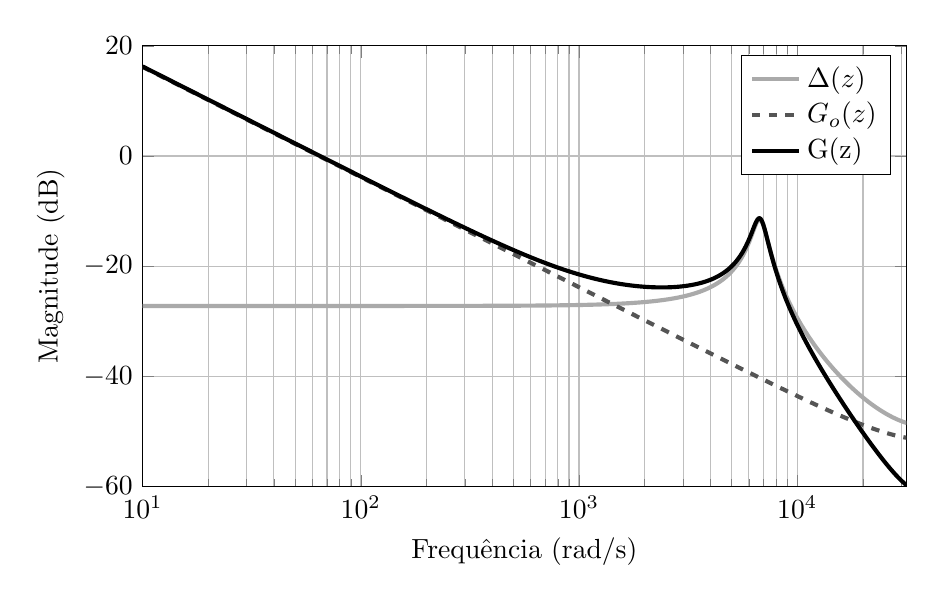
\begin{tikzpicture}

\begin{axis}[%
width=0.8\textwidth,
height=0.461611624834875\textwidth,
scale only axis,
xmode=log,
xmin=10,
xmax=31622.7766016838,
xminorticks=true,
xlabel={Frequência (rad/s)},
xmajorgrids,
xminorgrids,
ymin=-60,
ymax=20,
ylabel={Magnitude (dB)},
ymajorgrids,
legend style={draw=black,fill=white,legend cell align=left}
]
\addplot [color=mycolor1,solid,line width=1.5pt]
  table[row sep=crcr]{10	-27.220021747748\\
10.0461810465159	-27.2200215920221\\
10.0925753619375	-27.2200214348545\\
10.139183931163	-27.220021276232\\
10.1860077436388	-27.220021116141\\
10.2330477933808	-27.220020954568\\
10.2803050789954	-27.2200207914992\\
10.3277806037004	-27.2200206269208\\
10.375475375347	-27.2200204608188\\
10.4233904064403	-27.220020293179\\
10.4715267141616	-27.2200201239874\\
10.5198853203895	-27.2200199532294\\
10.5684672517218	-27.2200197808907\\
10.6172735394972	-27.2200196069565\\
10.6663052198171	-27.2200194314121\\
10.715563333568	-27.2200192542426\\
10.7650489264432	-27.2200190754329\\
10.814763048965	-27.2200188949679\\
10.8647067565072	-27.2200187128322\\
10.9148811093176	-27.2200185290104\\
10.9652871725401	-27.2200183434868\\
11.0159260162376	-27.2200181562458\\
11.0667987154147	-27.2200179672713\\
11.1179063500406	-27.2200177765474\\
11.1692500050717	-27.2200175840579\\
11.2208307704748	-27.2200173897863\\
11.2726497412507	-27.2200171937163\\
11.3247080174565	-27.2200169958312\\
11.3770067042298	-27.2200167961141\\
11.4295469118117	-27.2200165945482\\
11.4823297555707	-27.2200163911162\\
11.535356356026	-27.220016185801\\
11.5886278388715	-27.220015978585\\
11.6421453349997	-27.2200157694507\\
11.6959099805258	-27.2200155583803\\
11.7499229168114	-27.2200153453559\\
11.8041852904894	-27.2200151303595\\
11.8586982534876	-27.2200149133727\\
11.9134629630538	-27.2200146943771\\
11.96848058178	-27.2200144733542\\
12.0237522776272	-27.2200142502851\\
12.0792792239501	-27.2200140251509\\
12.135062599522	-27.2200137979326\\
12.1911035885602	-27.2200135686107\\
12.2474033807505	-27.2200133371659\\
12.3039631712731	-27.2200131035785\\
12.3607841608273	-27.2200128678286\\
12.4178675556577	-27.2200126298963\\
12.4752145675793	-27.2200123897613\\
12.5328264140034	-27.2200121474032\\
12.5907043179635	-27.2200119028014\\
12.6488495081411	-27.2200116559353\\
12.7072632188919	-27.2200114067837\\
12.765946690272	-27.2200111553257\\
12.8249011680643	-27.2200109015397\\
12.8841279038047	-27.2200106454043\\
12.9436281548089	-27.2200103868977\\
13.0034031841991	-27.2200101259979\\
13.0634542609305	-27.2200098626829\\
13.1237826598188	-27.2200095969301\\
13.1843896615665	-27.2200093287172\\
13.2452765527909	-27.2200090580213\\
13.306444626051	-27.2200087848193\\
13.3678951798747	-27.2200085090882\\
13.4296295187868	-27.2200082308045\\
13.4916489533366	-27.2200079499445\\
13.5539548001256	-27.2200076664845\\
13.6165483818355	-27.2200073804003\\
13.6794310272563	-27.2200070916676\\
13.7426040713143	-27.220006800262\\
13.806068855101	-27.2200065061587\\
13.8698267259009	-27.2200062093327\\
13.9338790372205	-27.2200059097588\\
13.998227148817	-27.2200056074116\\
14.062872426727	-27.2200053022653\\
14.1278162432955	-27.2200049942942\\
14.1930599772055	-27.2200046834719\\
14.2586050135065	-27.2200043697722\\
14.3244527436445	-27.2200040531685\\
14.3906045654914	-27.2200037336337\\
14.4570618833745	-27.2200034111408\\
14.5238261081064	-27.2200030856624\\
14.5908986570152	-27.2200027571708\\
14.658280953974	-27.2200024256382\\
14.7259744294318	-27.2200020910365\\
14.7939805204436	-27.2200017533371\\
14.8623006707006	-27.2200014125114\\
14.9309363305612	-27.2200010685305\\
14.999888957082	-27.2200007213652\\
15.069160014048	-27.2200003709859\\
15.1387509720044	-27.220000017363\\
15.2086633082875	-27.2199996604664\\
15.2788985070559	-27.2199993002658\\
15.3494580593225	-27.2199989367306\\
15.4203434629857	-27.2199985698299\\
15.4915562228612	-27.2199981995326\\
15.5630978507143	-27.2199978258073\\
15.6349698652918	-27.2199974486221\\
15.7071737923542	-27.2199970679451\\
15.779711164708	-27.219996683744\\
15.8525835222385	-27.2199962959861\\
15.9257924119422	-27.2199959046385\\
15.9993393879601	-27.2199955096679\\
16.07322601161	-27.2199951110409\\
16.1474538514202	-27.2199947087235\\
16.2220244831628	-27.2199943026817\\
16.2969394898867	-27.2199938928808\\
16.3722004619516	-27.2199934792862\\
16.4478089970617	-27.2199930618627\\
16.5237667002994	-27.2199926405749\\
16.6000751841599	-27.2199922153869\\
16.6767360685846	-27.2199917862627\\
16.7537509809962	-27.2199913531659\\
16.8311215563331	-27.2199909160596\\
16.9088494370839	-27.2199904749068\\
16.9869362733223	-27.2199900296699\\
17.0653837227424	-27.2199895803112\\
17.1441934506935	-27.2199891267925\\
17.2233671302159	-27.2199886690754\\
17.302906442076	-27.2199882071208\\
17.3828130748022	-27.2199877408897\\
17.4630887247206	-27.2199872703424\\
17.5437350959914	-27.2199867954389\\
17.6247539006444	-27.219986316139\\
17.7061468586161	-27.2199858324018\\
17.7879156977856	-27.2199853441865\\
17.8700621540116	-27.2199848514514\\
17.9525879711692	-27.2199843541548\\
18.035494901187	-27.2199838522544\\
18.1187847040838	-27.2199833457076\\
18.2024591480069	-27.2199828344713\\
18.2865200092687	-27.2199823185023\\
18.3709690723849	-27.2199817977566\\
18.4558081301122	-27.21998127219\\
18.5410389834868	-27.2199807417579\\
18.6266634418617	-27.2199802064153\\
18.7126833229461	-27.2199796661167\\
18.7991004528435	-27.2199791208162\\
18.8859166660905	-27.2199785704676\\
18.9731338056957	-27.219978015024\\
19.060753723179	-27.2199774544383\\
19.1487782786108	-27.2199768886629\\
19.2372093406515	-27.2199763176498\\
19.3260487865912	-27.2199757413504\\
19.4152985023894	-27.2199751597159\\
19.5049603827153	-27.2199745726969\\
19.5950363309877	-27.2199739802434\\
19.6855282594159	-27.2199733823052\\
19.7764380890397	-27.2199727788315\\
19.8677677497706	-27.2199721697711\\
19.9595191804325	-27.2199715550722\\
20.0516943288031	-27.2199709346827\\
20.1442951516552	-27.2199703085498\\
20.2373236147981	-27.2199696766204\\
20.3307816931193	-27.2199690388409\\
20.4246713706267	-27.219968395157\\
20.5189946404906	-27.2199677455141\\
20.6137535050858	-27.219967089857\\
20.7089499760343	-27.2199664281302\\
20.8045860742482	-27.2199657602772\\
20.900663829972	-27.2199650862416\\
20.9971852828265	-27.2199644059659\\
21.0941524818514	-27.2199637193925\\
21.1915674855492	-27.2199630264631\\
21.2894323619287	-27.2199623271187\\
21.387749188549	-27.2199616213001\\
21.4865200525637	-27.2199609089473\\
21.5857470507649	-27.2199601899997\\
21.685432289628	-27.2199594643964\\
21.7855778853565	-27.2199587320756\\
21.8861859639264	-27.2199579929753\\
21.987258661132	-27.2199572470327\\
22.0887981226306	-27.2199564941844\\
22.1908065039887	-27.2199557343665\\
22.2932859707273	-27.2199549675144\\
22.396238698368	-27.2199541935631\\
22.499666872479	-27.2199534124468\\
22.603572688722	-27.2199526240992\\
22.7079583528983	-27.2199518284534\\
22.8128260809959	-27.2199510254417\\
22.9181780992365	-27.219950214996\\
23.0240166441225	-27.2199493970475\\
23.130343962485	-27.2199485715267\\
23.237162311531	-27.2199477383634\\
23.3444739588916	-27.2199468974871\\
23.4522811826701	-27.2199460488261\\
23.5605862714901	-27.2199451923086\\
23.6693915245447	-27.2199443278616\\
23.7786992516445	-27.2199434554119\\
23.8885117732672	-27.2199425748854\\
23.9988314206069	-27.2199416862072\\
24.1096605356231	-27.219940789302\\
24.2210014710909	-27.2199398840934\\
24.3328565906507	-27.2199389705047\\
24.4452282688584	-27.2199380484583\\
24.558118891236	-27.2199371178759\\
24.6715308543219	-27.2199361786785\\
24.7854665657221	-27.2199352307863\\
24.899928444161	-27.2199342741187\\
25.0149189195332	-27.2199333085947\\
25.1304404329547	-27.2199323341321\\
25.2464954368146	-27.2199313506482\\
25.3630863948276	-27.2199303580596\\
25.4802157820863	-27.2199293562818\\
25.597886085113	-27.2199283452299\\
25.7160998019135	-27.219927324818\\
25.8348594420295	-27.2199262949594\\
25.9541675265918	-27.2199252555667\\
26.0740265883745	-27.2199242065516\\
26.194439171848	-27.2199231478251\\
26.3154078332332	-27.2199220792971\\
26.4369351405564	-27.219921000877\\
26.5590236737027	-27.2199199124733\\
26.6816760244719	-27.2199188139934\\
26.8048947966327	-27.2199177053441\\
26.9286826059784	-27.2199165864312\\
27.0530420803822	-27.2199154571597\\
27.1779758598533	-27.2199143174338\\
27.3034865965925	-27.2199131671566\\
27.4295769550488	-27.2199120062305\\
27.556249611976	-27.2199108345568\\
27.6835072564894	-27.2199096520361\\
27.8113525901229	-27.219908458568\\
27.9397883268864	-27.219907254051\\
28.0688171933232	-27.2199060383829\\
28.1984419285683	-27.2199048114605\\
28.3286652844062	-27.2199035731796\\
28.4594900253294	-27.2199023234351\\
28.5909189285972	-27.2199010621207\\
28.7229547842946	-27.2198997891294\\
28.8556003953913	-27.219898504353\\
28.9888585778017	-27.2198972076825\\
29.1227321604441	-27.2198958990078\\
29.2572239853012	-27.2198945782177\\
29.3923369074803	-27.2198932452001\\
29.5280737952738	-27.2198918998417\\
29.6644375302202	-27.2198905420283\\
29.8014310071653	-27.2198891716447\\
29.9390571343235	-27.2198877885743\\
30.0773188333397	-27.2198863926998\\
30.2162190393513	-27.2198849839026\\
30.3557607010504	-27.2198835620631\\
30.4959467807464	-27.2198821270606\\
30.6367802544292	-27.2198806787731\\
30.7782641118319	-27.2198792170778\\
30.9204013564946	-27.2198777418504\\
31.063195005828	-27.2198762529656\\
31.2066480911777	-27.2198747502971\\
31.350763657888	-27.2198732337172\\
31.4955447653674	-27.2198717030972\\
31.6409944871527	-27.219870158307\\
31.7871159109747	-27.2198685992155\\
31.9339121388238	-27.2198670256902\\
32.0813862870155	-27.2198654375976\\
32.229541486257	-27.2198638348028\\
32.3783808817133	-27.2198622171695\\
32.5279076330741	-27.2198605845606\\
32.6781249146208	-27.2198589368373\\
32.8290359152942	-27.2198572738597\\
32.9806438387618	-27.2198555954866\\
33.132951903486	-27.2198539015755\\
33.2859633427924	-27.2198521919824\\
33.4396814049384	-27.2198504665622\\
33.5941093531822	-27.2198487251684\\
33.7492504658521	-27.2198469676531\\
33.9051080364161	-27.2198451938671\\
34.0616853735517	-27.2198434036596\\
34.2189858012163	-27.2198415968788\\
34.3770126587175	-27.219839773371\\
34.5357693007845	-27.2198379329815\\
34.6952590976386	-27.2198360755541\\
34.8554854350656	-27.2198342009308\\
35.0164517144866	-27.2198323089526\\
35.1781613530314	-27.2198303994588\\
35.3406177836102	-27.2198284722871\\
35.5038244549868	-27.219826527274\\
35.6677848318515	-27.2198245642543\\
35.8325023948954	-27.2198225830612\\
35.9979806408833	-27.2198205835265\\
36.1642230827288	-27.2198185654804\\
36.3312332495683	-27.2198165287515\\
36.4990146868361	-27.2198144731668\\
36.6675709563398	-27.2198123985519\\
36.8369056363357	-27.2198103047304\\
37.007022321605	-27.2198081915245\\
37.1779246235299	-27.2198060587549\\
37.3496161701703	-27.2198039062403\\
37.5221006063408	-27.219801733798\\
37.6953815936883	-27.2197995412435\\
37.8694628107696	-27.2197973283905\\
38.0443479531292	-27.2197950950512\\
38.2200407333782	-27.2197928410359\\
38.3965448812729	-27.2197905661531\\
38.5738641437941	-27.2197882702097\\
38.7520022852263	-27.2197859530106\\
38.9309630872381	-27.2197836143591\\
39.1107503489621	-27.2197812540566\\
39.2913678870758	-27.2197788719026\\
39.4728195358824	-27.2197764676948\\
39.6551091473924	-27.219774041229\\
39.8382405914052	-27.2197715922992\\
40.0222177555915	-27.2197691206974\\
40.2070445455755	-27.2197666262136\\
40.3927248850181	-27.219764108636\\
40.5792627157	-27.2197615677509\\
40.7666619976054	-27.2197590033424\\
40.9549267090063	-27.2197564151927\\
41.1440608465467	-27.2197538030821\\
41.3340684253274	-27.2197511667886\\
41.5249534789915	-27.2197485060884\\
41.7167200598098	-27.2197458207556\\
41.9093722387671	-27.219743110562\\
42.1029141056481	-27.2197403752775\\
42.2973497691249	-27.2197376146699\\
42.4926833568435	-27.2197348285045\\
42.6889190155123	-27.2197320165449\\
42.8860609109892	-27.2197291785522\\
43.0841132283705	-27.2197263142854\\
43.2830801720801	-27.2197234235012\\
43.4829659659579	-27.2197205059541\\
43.6837748533501	-27.2197175613963\\
43.8855110971994	-27.2197145895778\\
44.0881789801347	-27.2197115902461\\
44.2917828045629	-27.2197085631466\\
44.4963268927599	-27.2197055080221\\
44.701815586962	-27.2197024246131\\
44.9082532494586	-27.2196993126579\\
45.1156442626847	-27.219696171892\\
45.3239930293136	-27.2196930020489\\
45.5333039723509	-27.2196898028591\\
45.7435815352278	-27.2196865740511\\
45.954830181896	-27.2196833153506\\
46.167054396922	-27.2196800264808\\
46.3802586855826	-27.2196767071625\\
46.5944475739604	-27.2196733571136\\
46.8096256090399	-27.2196699760498\\
47.0257973588042	-27.2196665636838\\
47.2429674123316	-27.2196631197258\\
47.4611403798933	-27.2196596438833\\
47.6803208930514	-27.2196561358612\\
47.9005136047569	-27.2196525953614\\
48.1217231894485	-27.2196490220833\\
48.3439543431522	-27.2196454157233\\
48.5672117835806	-27.2196417759753\\
48.791500250233	-27.21963810253\\
49.0168245044966	-27.2196343950755\\
49.243189329747	-27.2196306532969\\
49.4705995314498	-27.2196268768764\\
49.6990599372628	-27.2196230654932\\
49.9285753971387	-27.2196192188236\\
50.1591507834275	-27.219615336541\\
50.3907909909802	-27.2196114183156\\
50.6235009372529	-27.2196074638145\\
50.8572855624109	-27.2196034727021\\
51.0921498294339	-27.2195994446391\\
51.3280987242209	-27.2195953792836\\
51.5651372556965	-27.2195912762903\\
51.8032704559168	-27.2195871353107\\
52.0425033801768	-27.219582955993\\
52.2828411071172	-27.2195787379823\\
52.5242887388322	-27.2195744809203\\
52.7668514009784	-27.2195701844455\\
53.010534242883	-27.219565848193\\
53.2553424376533	-27.2195614717944\\
53.5012811822866	-27.219557054878\\
53.7483556977805	-27.2195525970687\\
53.9965712292437	-27.2195480979879\\
54.2459330460073	-27.2195435572534\\
54.4964464417369	-27.2195389744796\\
54.7481167345445	-27.2195343492772\\
55.0009492671021	-27.2195296812533\\
55.2549494067543	-27.2195249700116\\
55.510122545633	-27.2195202151517\\
55.7664741007712	-27.2195154162699\\
56.0240095142187	-27.2195105729586\\
56.282734253157	-27.2195056848064\\
56.5426538100157	-27.219500751398\\
56.8037737025889	-27.2194957723145\\
57.0660994741527	-27.219490747133\\
57.3296366935823	-27.2194856754266\\
57.5943909554708	-27.2194805567645\\
57.8603678802477	-27.219475390712\\
58.1275731142982	-27.2194701768303\\
58.3960123300829	-27.2194649146765\\
58.6656912262587	-27.2194596038036\\
58.9366155277994	-27.2194542437606\\
59.2087909861172	-27.2194488340921\\
59.4822233791852	-27.2194433743387\\
59.7569185116595	-27.2194378640367\\
60.0328822150028	-27.2194323027179\\
60.3101203476082	-27.21942668991\\
60.5886387949234	-27.2194210251362\\
60.8684434695757	-27.2194153079155\\
61.1495403114975	-27.219409537762\\
61.4319352880526	-27.2194037141858\\
61.7156343941624	-27.2193978366921\\
62.0006436524339	-27.2193919047818\\
62.2869691132868	-27.2193859179509\\
62.5746168550822	-27.2193798756909\\
62.8635929842521	-27.2193737774885\\
63.1539036354283	-27.2193676228259\\
63.445554971573	-27.2193614111801\\
63.7385531841099	-27.2193551420235\\
64.032904493055	-27.2193488148236\\
64.3286151471491	-27.219342429043\\
64.6256914239905	-27.2193359841392\\
64.9241396301678	-27.2193294795648\\
65.2239661013943	-27.2193229147672\\
65.5251772026422	-27.2193162891888\\
65.827779328278	-27.2193096022668\\
66.1317789021976	-27.2193028534331\\
66.4371823779638	-27.2192960421145\\
66.7439962389419	-27.2192891677324\\
67.0522269984386	-27.2192822297028\\
67.3618811998395	-27.2192752274364\\
67.6729654167483	-27.2192681603383\\
67.9854862531262	-27.2192610278083\\
68.2994503434323	-27.2192538292403\\
68.6148643527643	-27.219246564023\\
68.931734977	-27.2192392315392\\
69.2500689429393	-27.2192318311659\\
69.5698730084476	-27.2192243622746\\
69.8911539625984	-27.2192168242307\\
70.213918625818	-27.219209216394\\
70.5381738500302	-27.2192015381181\\
70.8639265188016	-27.2191937887507\\
71.191183547488	-27.2191859676336\\
71.5199518833808	-27.2191780741023\\
71.8502385058548	-27.2191701074864\\
72.1820504265165	-27.2191620671089\\
72.5153946893524	-27.2191539522869\\
72.8502783708792	-27.219145762331\\
73.1867085802933	-27.2191374965455\\
73.5246924596224	-27.2191291542282\\
73.8642371838769	-27.2191207346702\\
74.2053499612018	-27.2191122371565\\
74.5480380330304	-27.2191036609651\\
74.8923086742377	-27.2190950053674\\
75.2381691932944	-27.2190862696281\\
75.585626932423	-27.219077453005\\
75.9346892677529	-27.2190685547492\\
76.2853636094773	-27.2190595741047\\
76.6376574020103	-27.2190505103085\\
76.9915781241455	-27.2190413625906\\
77.3471332892138	-27.2190321301739\\
77.7043304452438	-27.219022812274\\
78.0631771751216	-27.2190134080993\\
78.4236810967518	-27.2190039168507\\
78.7858498632195	-27.2189943377221\\
79.1496911629522	-27.2189846698995\\
79.5152127198837	-27.2189749125616\\
79.8824222936175	-27.2189650648795\\
80.2513276795919	-27.2189551260164\\
80.6219367092452	-27.2189450951279\\
80.9942572501823	-27.2189349713619\\
81.3682972063414	-27.2189247538582\\
81.7440645181619	-27.2189144417488\\
82.121567162753	-27.2189040341574\\
82.5008131540631	-27.2188935301999\\
82.8818105430498	-27.2188829289838\\
83.2645674178507	-27.2188722296085\\
83.6490919039556	-27.2188614311648\\
84.0353921643786	-27.2188505327352\\
84.423476399831	-27.2188395333939\\
84.8133528488963	-27.2188284322063\\
85.2050297882047	-27.2188172282291\\
85.5985155326084	-27.2188059205104\\
85.9938184353586	-27.2187945080894\\
86.3909468882829	-27.2187829899965\\
86.7899093219629	-27.2187713652531\\
87.1907142059136	-27.2187596328713\\
87.5933700487633	-27.2187477918543\\
87.9978853984339	-27.2187358411961\\
88.4042688423224	-27.2187237798811\\
88.8125290074835	-27.2187116068846\\
89.2226745608124	-27.2186993211722\\
89.6347142092288	-27.2186869217\\
90.0486566998624	-27.2186744074145\\
90.4645108202374	-27.2186617772521\\
90.88228539846	-27.2186490301399\\
91.3019893034057	-27.2186361649945\\
91.7236314449071	-27.2186231807229\\
92.1472207739435	-27.2186100762217\\
92.5727662828307	-27.2185968503773\\
93.0002770054119	-27.218583502066\\
93.4297620172496	-27.2185700301534\\
93.8612304358183	-27.2185564334948\\
94.2946914206979	-27.2185427109348\\
94.730154173768	-27.2185288613073\\
95.1676279394036	-27.2185148834354\\
95.6071220046713	-27.2185007761313\\
96.0486456995261	-27.2184865381961\\
96.4922083970099	-27.2184721684201\\
96.9378195134503	-27.2184576655819\\
97.3854885086602	-27.2184430284493\\
97.8352248861393	-27.2184282557783\\
98.2870381932753	-27.2184133463135\\
98.7409380215466	-27.2183982987879\\
99.1969340067261	-27.2183831119227\\
99.655035829086	-27.2183677844273\\
100.115253213603	-27.2183523149991\\
100.577595930163	-27.2183367023235\\
101.042073793774	-27.2183209450737\\
101.508696664767	-27.2183050419104\\
101.977474449012	-27.2182889914822\\
102.448417098122	-27.218272792425\\
102.921534609671	-27.218256443362\\
103.3968370274	-27.2182399429039\\
103.874334441436	-27.2182232896481\\
104.354036988501	-27.2182064821795\\
104.83595485213	-27.2181895190696\\
105.320098262886	-27.2181723988765\\
105.80647749858	-27.2181551201453\\
106.295102884484	-27.2181376814075\\
106.785984793556	-27.2181200811808\\
107.279133646656	-27.2181023179693\\
107.774559912768	-27.2180843902633\\
108.272274109224	-27.218066296539\\
108.772286801926	-27.2180480352586\\
109.27460860557	-27.2180296048698\\
109.779250183872	-27.2180110038062\\
110.286222249794	-27.2179922304868\\
110.795535565772	-27.2179732833157\\
111.307200943943	-27.2179541606825\\
111.821229246378	-27.2179348609619\\
112.337631385307	-27.2179153825132\\
112.856418323356	-27.2178957236808\\
113.377601073777	-27.2178758827937\\
113.901190700682	-27.2178558581652\\
114.427198319278	-27.2178356480933\\
114.955635096105	-27.21781525086\\
115.486512249268	-27.2177946647314\\
116.019841048683	-27.2177738879575\\
116.555632816306	-27.2177529187722\\
117.093898926384	-27.2177317553929\\
117.634650805689	-27.2177103960206\\
118.177899933763	-27.2176888388394\\
118.723657843162	-27.2176670820167\\
119.271936119701	-27.2176451237031\\
119.822746402699	-27.2176229620318\\
120.376100385228	-27.2176005951187\\
120.932009814357	-27.2175780210623\\
121.490486491407	-27.2175552379435\\
122.051542272196	-27.2175322438253\\
122.615189067297	-27.2175090367529\\
123.181438842284	-27.2174856147532\\
123.750303617991	-27.2174619758349\\
124.321795470765	-27.2174381179882\\
124.895926532723	-27.2174140391848\\
125.472708992008	-27.2173897373774\\
126.052155093052	-27.2173652104998\\
126.63427713683	-27.2173404564665\\
127.219087481126	-27.217315473173\\
127.806598540793	-27.217290258495\\
128.396822788018	-27.2172648102885\\
128.989772752585	-27.2172391263898\\
129.585461022141	-27.217213204615\\
130.183900242466	-27.2171870427599\\
130.785103117737	-27.2171606385999\\
131.389082410804	-27.21713398989\\
131.995850943453	-27.217107094364\\
132.605421596686	-27.2170799497349\\
133.217807310988	-27.2170525536944\\
133.833021086605	-27.217024903913\\
134.451075983821	-27.2169969980393\\
135.071985123233	-27.2169688337002\\
135.69576168603	-27.2169404085006\\
136.322418914273	-27.2169117200233\\
136.951970111177	-27.2168827658285\\
137.584428641392	-27.2168535434539\\
138.219807931287	-27.2168240504142\\
138.858121469236	-27.2167942842011\\
139.499382805904	-27.2167642422833\\
140.143605554534	-27.2167339221056\\
140.790803391236	-27.2167033210893\\
141.440990055278	-27.2166724366319\\
142.094179349378	-27.2166412661064\\
142.750385139995	-27.2166098068619\\
143.409621357626	-27.2165780562225\\
144.0719019971	-27.2165460114876\\
144.737241117876	-27.2165136699317\\
145.405652844341	-27.2164810288038\\
146.077151366109	-27.2164480853274\\
146.751750938323	-27.2164148367005\\
147.42946588196	-27.2163812800947\\
148.110310584131	-27.2163474126556\\
148.794299498388	-27.2163132315024\\
149.481447145032	-27.2162787337272\\
150.171768111418	-27.2162439163955\\
150.865277052271	-27.2162087765455\\
151.561988689989	-27.2161733111876\\
152.261917814963	-27.2161375173049\\
152.965079285884	-27.2161013918522\\
153.671488030065	-27.2160649317561\\
154.381159043753	-27.2160281339148\\
155.094107392451	-27.2159909951975\\
155.810348211234	-27.2159535124446\\
156.529896705074	-27.2159156824669\\
157.25276814916	-27.2158775020459\\
157.978977889225	-27.2158389679329\\
158.708541341869	-27.2158000768492\\
159.441473994887	-27.2157608254858\\
160.177791407599	-27.2157212105027\\
160.917509211179	-27.2156812285292\\
161.66064310899	-27.2156408761631\\
162.40720887691	-27.2156001499707\\
163.157222363676	-27.2155590464863\\
163.910699491214	-27.2155175622122\\
164.66765625498	-27.2154756936181\\
165.428108724297	-27.2154334371411\\
166.192073042701	-27.215390789185\\
166.959565428276	-27.2153477461203\\
167.730602174008	-27.2153043042838\\
168.505199648122	-27.2152604599783\\
169.283374294433	-27.2152162094723\\
170.065142632699	-27.2151715489995\\
170.850521258965	-27.2151264747589\\
171.639526845917	-27.2150809829139\\
172.432176143241	-27.2150350695925\\
173.228485977972	-27.2149887308866\\
174.028473254854	-27.2149419628519\\
174.832154956701	-27.2148947615074\\
175.639548144754	-27.2148471228351\\
176.450669959044	-27.2147990427798\\
177.265537618758	-27.2147505172485\\
178.084168422602	-27.2147015421103\\
178.906579749169	-27.2146521131958\\
179.732789057308	-27.214602226297\\
180.562813886497	-27.2145518771668\\
181.39667185721	-27.2145010615186\\
182.234380671297	-27.2144497750259\\
183.075958112354	-27.2143980133221\\
183.921422046107	-27.214345772\\
184.770790420785	-27.2142930466116\\
185.624081267505	-27.2142398326672\\
186.481312700654	-27.2141861256359\\
187.342502918271	-27.2141319209442\\
188.207670202438	-27.2140772139765\\
189.076832919665	-27.214022000074\\
189.950009521279	-27.2139662745348\\
190.827218543818	-27.2139100326133\\
191.708478609426	-27.2138532695196\\
192.593808426241	-27.2137959804196\\
193.483226788801	-27.2137381604339\\
194.376752578439	-27.2136798046382\\
195.274404763682	-27.213620908062\\
196.176202400658	-27.2135614656888\\
197.082164633495	-27.2135014724555\\
197.992310694735	-27.2134409232518\\
198.906659905733	-27.21337981292\\
199.825231677076	-27.2133181362545\\
200.748045508988	-27.2132558880012\\
201.675120991751	-27.2131930628571\\
202.606477806113	-27.21312965547\\
203.542135723711	-27.213065660438\\
204.482114607491	-27.2130010723087\\
205.426434412127	-27.2129358855794\\
206.375115184445	-27.2128700946959\\
207.32817706385	-27.2128036940524\\
208.285640282755	-27.2127366779911\\
209.247525167004	-27.2126690408015\\
210.213852136311	-27.21260077672\\
211.18464170469	-27.2125318799293\\
212.159914480891	-27.2124623445582\\
213.139691168835	-27.2123921646807\\
214.123992568061	-27.2123213343157\\
215.112839574156	-27.2122498474266\\
216.10625317921	-27.2121776979204\\
217.104254472254	-27.2121048796476\\
218.106864639713	-27.2120313864015\\
219.114104965849	-27.2119572119175\\
220.12599683322	-27.2118823498729\\
221.142561723131	-27.2118067938859\\
222.163821216089	-27.2117305375156\\
223.189796992262	-27.211653574261\\
224.220510831939	-27.2115758975606\\
225.255984615994	-27.2114975007918\\
226.296240326348	-27.2114183772706\\
227.341300046436	-27.2113385202504\\
228.391185961678	-27.2112579229222\\
229.44592035995	-27.2111765784132\\
230.505525632052	-27.211094479787\\
231.570024272191	-27.2110116200424\\
232.639438878451	-27.2109279921131\\
233.713792153278	-27.210843588867\\
234.793106903962	-27.2107584031055\\
235.877406043117	-27.2106724275631\\
236.966712589169	-27.2105856549065\\
238.061049666849	-27.2104980777343\\
239.160440507677	-27.210409688576\\
240.264908450462	-27.2103204798915\\
241.374476941791	-27.2102304440707\\
242.48916953653	-27.2101395734323\\
243.609009898327	-27.2100478602237\\
244.734021800108	-27.2099552966199\\
245.864229124585	-27.2098618747232\\
246.999655864764	-27.209767586562\\
248.140326124455	-27.2096724240908\\
249.286264118777	-27.2095763791888\\
250.437494174681	-27.2094794436597\\
251.594040731461	-27.2093816092309\\
252.755928341275	-27.2092828675524\\
253.923181669665	-27.2091832101967\\
255.09582549608	-27.2090826286575\\
256.273884714404	-27.2089811143494\\
257.457384333485	-27.2088786586069\\
258.646349477661	-27.2087752526835\\
259.840805387301	-27.2086708877515\\
261.040777419332	-27.2085655549007\\
262.246291047787	-27.2084592451379\\
263.457371864337	-27.2083519493858\\
264.674045578839	-27.2082436584828\\
265.896338019882	-27.2081343631817\\
267.124275135332	-27.2080240541488\\
268.357882992886	-27.2079127219638\\
269.597187780627	-27.2078003571182\\
270.842215807572	-27.2076869500149\\
272.092993504239	-27.2075724909672\\
273.349547423206	-27.2074569701981\\
274.611904239671	-27.2073403778394\\
275.880090752022	-27.2072227039306\\
277.154133882405	-27.2071039384184\\
278.434060677294	-27.2069840711558\\
279.719898308069	-27.2068630919009\\
281.011674071587	-27.2067409903161\\
282.309415390768	-27.2066177559675\\
283.613149815172	-27.2064933783239\\
284.922905021585	-27.2063678467553\\
286.238708814609	-27.206241150533\\
287.560589127251	-27.2061132788278\\
288.888574021513	-27.2059842207093\\
290.222691688993	-27.2058539651451\\
291.562970451479	-27.205722501\\
292.909438761552	-27.2055898170345\\
294.262125203191	-27.205455901904\\
295.621058492378	-27.2053207441583\\
296.98626747771	-27.2051843322398\\
298.357781141006	-27.2050466544832\\
299.735628597932	-27.2049076991141\\
301.119839098607	-27.2047674542479\\
302.510442028234	-27.2046259078892\\
303.907466907719	-27.2044830479303\\
305.310943394298	-27.2043388621502\\
306.720901282168	-27.2041933382139\\
308.137370503119	-27.204046463671\\
309.560381127168	-27.2038982259544\\
310.989963363199	-27.2037486123799\\
312.426147559604	-27.2035976101443\\
313.868964204927	-27.2034452063249\\
315.318443928511	-27.203291387878\\
316.774617501149	-27.2031361416379\\
318.237515835737	-27.2029794543157\\
319.707169987928	-27.2028213124981\\
321.183611156796	-27.2026617026464\\
322.666870685493	-27.2025006110951\\
324.156980061919	-27.2023380240508\\
325.653970919389	-27.202173927591\\
327.1578750373	-27.2020083076629\\
328.668724341813	-27.201841150082\\
330.186550906528	-27.2016724405311\\
331.711386953162	-27.2015021645589\\
333.243264852235	-27.2013303075787\\
334.78221712376	-27.2011568548672\\
336.328276437929	-27.2009817915632\\
337.881475615808	-27.2008051026662\\
339.441847630035	-27.2006267730352\\
341.009425605519	-27.2004467873874\\
342.584242820144	-27.2002651302965\\
344.166332705473	-27.200081786192\\
345.75572884746	-27.199896739357\\
347.352464987164	-27.1997099739276\\
348.956575021463	-27.1995214738911\\
350.568093003772	-27.1993312230844\\
352.187053144771	-27.1991392051931\\
353.813489813129	-27.1989454037497\\
355.447437536229	-27.1987498021321\\
357.088931000911	-27.1985523835625\\
358.738005054198	-27.1983531311053\\
360.39469470404	-27.1981520276664\\
362.059035120061	-27.197949055991\\
363.731061634299	-27.1977441986624\\
365.410809741959	-27.1975374381004\\
367.09831510217	-27.1973287565597\\
368.793613538734	-27.1971181361285\\
370.496741040893	-27.1969055587266\\
372.207733764093	-27.1966910061042\\
373.926628030746	-27.1964744598399\\
375.653460331008	-27.1962559013393\\
377.388267323548	-27.1960353118332\\
379.13108583633	-27.1958126723761\\
380.881952867393	-27.1955879638445\\
382.640905585636	-27.1953611669349\\
384.407981331609	-27.1951322621625\\
386.183217618305	-27.1949012298594\\
387.966652131954	-27.1946680501725\\
389.758322732826	-27.194432703062\\
391.558267456034	-27.1941951682998\\
393.366524512341	-27.1939554254672\\
395.183132288971	-27.1937134539536\\
397.008129350424	-27.1934692329544\\
398.841554439296	-27.193222741469\\
400.683446477099	-27.1929739582993\\
402.533844565089	-27.1927228620476\\
404.392787985098	-27.1924694311145\\
406.260316200361	-27.1922136436975\\
408.136468856361	-27.1919554777885\\
410.021285781671	-27.191694911172\\
411.914806988789	-27.1914319214234\\
413.817072675003	-27.1911664859066\\
415.72812322323	-27.1908985817722\\
417.647999202884	-27.1906281859554\\
419.576741370729	-27.1903552751738\\
421.514390671752	-27.1900798259257\\
423.460988240025	-27.1898018144874\\
425.416575399583	-27.1895212169117\\
427.381193665299	-27.1892380090252\\
429.354884743766	-27.1889521664267\\
431.337690534184	-27.1886636644843\\
433.329653129246	-27.1883724783338\\
435.330814816033	-27.1880785828763\\
437.341218076915	-27.1877819527756\\
439.360905590448	-27.1874825624566\\
441.389920232282	-27.1871803861021\\
443.428305076071	-27.1868753976514\\
445.476103394389	-27.1865675707973\\
447.533358659646	-27.186256878984\\
449.600114545014	-27.1859432954045\\
451.67641492535	-27.1856267929985\\
453.762303878129	-27.1853073444497\\
455.857825684385	-27.1849849221834\\
457.963024829641	-27.184659498364\\
460.077946004862	-27.1843310448924\\
462.202634107401	-27.1839995334038\\
464.33713424195	-27.1836649352645\\
466.481491721497	-27.18332722157\\
468.635752068297	-27.1829863631419\\
470.799961014824	-27.1826423305253\\
472.974164504755	-27.1822950939864\\
475.158408693936	-27.1819446235096\\
477.352739951367	-27.1815908887946\\
479.557204860185	-27.1812338592539\\
481.771850218653	-27.1808735040102\\
483.996723041153	-27.180509791893\\
486.231870559183	-27.1801426914362\\
488.477340222363	-27.179772170875\\
490.73317969944	-27.1793981981434\\
492.999436879299	-27.1790207408707\\
495.276159871982	-27.1786397663789\\
497.563397009708	-27.1782552416797\\
499.861196847899	-27.1778671334712\\
502.169608166212	-27.1774754081354\\
504.48867996957	-27.1770800317345\\
506.818461489212	-27.1766809700081\\
509.159002183727	-27.17627818837\\
511.51035174011	-27.1758716519052\\
513.872560074817	-27.1754613253663\\
516.245677334823	-27.1750471731708\\
518.629753898685	-27.174629159397\\
521.024840377617	-27.1742072477817\\
523.430987616559	-27.1737814017161\\
525.848246695256	-27.1733515842428\\
528.27666892935	-27.172917758052\\
530.716305871459	-27.1724798854786\\
533.167209312278	-27.1720379284983\\
535.629431281677	-27.1715918487243\\
538.103024049808	-27.1711416074035\\
540.588040128206	-27.1706871654133\\
543.084532270915	-27.1702284832574\\
545.592553475602	-27.1697655210628\\
548.11215698468	-27.1692982385755\\
550.643396286443	-27.1688265951573\\
553.186325116201	-27.1683505497814\\
555.740997457415	-27.1678700610291\\
558.307467542852	-27.1673850870859\\
560.885789855729	-27.1668955857372\\
563.476019130871	-27.1664015143647\\
566.078210355879	-27.1659028299424\\
568.692418772287	-27.1653994890324\\
571.318699876742	-27.164891447781\\
573.957109422183	-27.1643786619145\\
576.607703419019	-27.1638610867352\\
579.27053813632	-27.1633386771169\\
581.945670103016	-27.162811387501\\
584.633156109091	-27.1622791718919\\
587.333053206791	-27.1617419838531\\
590.045418711838	-27.1611997765024\\
592.77031020464	-27.1606525025075\\
595.507785531519	-27.1601001140819\\
598.25790280594	-27.1595425629802\\
601.020720409738	-27.1589798004932\\
603.796296994364	-27.158411777444\\
606.584691482126	-27.1578384441827\\
609.385963067442	-27.1572597505819\\
612.200171218097	-27.156675646032\\
615.027375676503	-27.1560860794365\\
617.867636460969	-27.155490999207\\
620.721013866976	-27.1548903532581\\
623.587568468455	-27.1542840890028\\
626.467361119072	-27.1536721533474\\
629.360452953524	-27.1530544926861\\
632.266905388836	-27.1524310528964\\
635.186780125658	-27.1518017793335\\
638.120139149584	-27.1511666168252\\
641.067044732464	-27.150525509667\\
644.027559433723	-27.1498784016158\\
647.001746101695	-27.1492252358855\\
649.989667874954	-27.1485659551412\\
652.991388183652	-27.1479005014932\\
656.00697075087	-27.1472288164923\\
659.03647959397	-27.1465508411233\\
662.07997902595	-27.1458665158\\
665.137533656814	-27.145175780359\\
668.209208394941	-27.144478574054\\
671.295068448464	-27.14377483555\\
674.395179326655	-27.1430645029172\\
677.509606841313	-27.1423475136251\\
680.638417108163	-27.1416238045364\\
683.78167654826	-27.1408933119008\\
686.9394518894	-27.1401559713488\\
690.11181016753	-27.1394117178856\\
693.298818728181	-27.1386604858843\\
696.500545227891	-27.1379022090801\\
699.717057635642	-27.1371368205633\\
702.948424234306	-27.1363642527729\\
706.19471362209	-27.1355844374901\\
709.455994713995	-27.1347973058314\\
712.732336743282	-27.1340027882419\\
716.023809262934	-27.1332008144885\\
719.330482147139	-27.1323913136529\\
722.652425592773	-27.1315742141246\\
725.989710120886	-27.1307494435939\\
729.3424065782	-27.1299169290446\\
732.71058613862	-27.1290765967468\\
736.094320304735	-27.1282283722497\\
739.493680909343	-27.127372180374\\
742.908740116972	-27.1265079452046\\
746.339570425412	-27.1256355900828\\
749.786244667258	-27.124755037599\\
753.248836011454	-27.1238662095845\\
756.727417964843	-27.1229690271041\\
760.222064373731	-27.122063410448\\
763.732849425456	-27.1211492791237\\
767.259847649959	-27.120226551848\\
770.803133921369	-27.119295146539\\
774.362783459591	-27.1183549803074\\
777.938871831903	-27.1174059694486\\
781.531474954562	-27.1164480294338\\
785.140669094413	-27.1154810749017\\
788.76653087051	-27.1145050196499\\
792.40913725574	-27.1135197766259\\
796.068565578463	-27.1125252579184\\
799.744893524145	-27.1115213747483\\
803.438199137013	-27.1105080374597\\
807.148560821713	-27.1094851555107\\
810.876057344967	-27.1084526374639\\
814.620767837254	-27.1074103909774\\
818.382771794484	-27.1063583227953\\
822.162149079689	-27.1052963387377\\
825.958979924714	-27.1042243436912\\
829.773344931927	-27.1031422415996\\
833.605325075921	-27.1020499354529\\
837.455001705243	-27.1009473272783\\
841.322456544116	-27.0998343181294\\
845.207771694168	-27.0987108080763\\
849.111029636188	-27.0975766961948\\
853.032313231867	-27.0964318805562\\
856.971705725559	-27.0952762582166\\
860.92929074605	-27.094109725206\\
864.905152308334	-27.0929321765177\\
868.899374815392	-27.0917435060968\\
872.91204305999	-27.0905436068295\\
876.943242226474	-27.0893323705315\\
880.993057892579	-27.088109687937\\
885.061576031251	-27.0868754486866\\
889.148883012464	-27.0856295413159\\
893.255065605058	-27.0843718532438\\
897.380210978585	-27.0831022707604\\
901.52440670515	-27.0818206790147\\
905.687740761275	-27.0805269620027\\
909.870301529772	-27.0792210025548\\
914.07217780161	-27.0779026823231\\
918.293458777803	-27.0765718817691\\
922.534234071309	-27.0752284801506\\
926.794593708924	-27.0738723555086\\
931.074628133199	-27.0725033846544\\
935.374428204358	-27.071121443156\\
939.694085202226	-27.0697264053249\\
944.033690828168	-27.0683181442021\\
948.39333720704	-27.0668965315448\\
952.773116889131	-27.0654614378118\\
957.173122852146	-27.0640127321498\\
961.593448503166	-27.0625502823791\\
966.034187680636	-27.0610739549786\\
970.495434656357	-27.0595836150718\\
974.977284137491	-27.0580791264114\\
979.479831268559	-27.0565603513646\\
984.003171633478	-27.0550271508975\\
988.547401257578	-27.0534793845604\\
993.112616609642	-27.0519169104712\\
997.698914603958	-27.0503395853006\\
1002.30639260238	-27.0487472642552\\
1006.93514841637	-27.0471398010622\\
1011.58528030912	-27.0455170479522\\
1016.2568869976	-27.0438788556431\\
1020.95006765465	-27.0422250733233\\
1025.66492191112	-27.0405555486342\\
1030.40154985798	-27.0388701276536\\
1035.16005204838	-27.0371686548778\\
1039.94052949988	-27.0354509732042\\
1044.74308369654	-27.0337169239133\\
1049.56781659108	-27.0319663466503\\
1054.41483060703	-27.0301990794075\\
1059.28422864096	-27.0284149585049\\
1064.17611406461	-27.0266138185718\\
1069.09059072708	-27.0247954925277\\
1074.02776295708	-27.0229598115632\\
1078.98773556513	-27.0211066051197\\
1083.97061384575	-27.0192357008707\\
1088.97650357974	-27.0173469247008\\
1094.00551103639	-27.0154401006858\\
1099.05774297578	-27.0135150510722\\
1104.13330665098	-27.011571596256\\
1109.2323098104	-27.0096095547622\\
1114.35486070002	-27.0076287432225\\
1119.50106806574	-27.0056289763546\\
1124.67104115564	-27.0036100669396\\
1129.86488972231	-27.0015718257999\\
1135.0827240252	-26.9995140617768\\
1140.32465483296	-26.9974365817077\\
1145.59079342577	-26.9953391904027\\
1150.8812515977	-26.9932216906213\\
1156.19614165913	-26.9910838830489\\
1161.53557643908	-26.9889255662723\\
1166.89966928762	-26.9867465367556\\
1172.28853407829	-26.9845465888154\\
1177.70228521052	-26.982325514596\\
1183.14103761204	-26.9800831040435\\
1188.60490674132	-26.9778191448807\\
1194.09400859005	-26.9755334225805\\
1199.60845968555	-26.9732257203398\\
1205.14837709331	-26.9708958190527\\
1210.71387841942	-26.9685434972834\\
1216.30508181309	-26.9661685312385\\
1221.92210596917	-26.9637706947394\\
1227.56507013062	-26.9613497591936\\
1233.23409409112	-26.9589054935669\\
1238.92929819754	-26.9564376643532\\
1244.65080335254	-26.9539460355461\\
1250.3987310171	-26.9514303686087\\
1256.17320321316	-26.9488904224429\\
1261.97434252612	-26.9463259533596\\
1267.80227210752	-26.9437367150468\\
1273.65711567764	-26.9411224585386\\
1279.53899752808	-26.9384829321831\\
1285.44804252445	-26.9358178816096\\
1291.38437610901	-26.9331270496965\\
1297.34812430331	-26.9304101765372\\
1303.33941371088	-26.9276669994068\\
1309.35837151994	-26.9248972527276\\
1315.40512550606	-26.9221006680345\\
1321.47980403488	-26.9192769739395\\
1327.58253606487	-26.9164258960963\\
1333.71345115004	-26.9135471571636\\
1339.87267944269	-26.9106404767686\\
1346.06035169616	-26.9077055714698\\
1352.27659926764	-26.9047421547189\\
1358.52155412096	-26.9017499368224\\
1364.79534882933	-26.8987286249028\\
1371.09811657822	-26.8956779228593\\
1377.42999116818	-26.8925975313271\\
1383.79110701763	-26.8894871476373\\
1390.18159916578	-26.8863464657755\\
1396.60160327544	-26.8831751763397\\
1403.05125563594	-26.8799729664983\\
1409.53069316601	-26.8767395199465\\
1416.04005341668	-26.8734745168629\\
1422.5794745742	-26.8701776338648\\
1429.14909546299	-26.8668485439638\\
1435.74905554856	-26.8634869165191\\
1442.3794949405	-26.8600924171923\\
1449.04055439544	-26.8566647078992\\
1455.73237532004	-26.8532034467629\\
1462.45509977397	-26.8497082880646\\
1469.20887047298	-26.8461788821949\\
1475.99383079187	-26.8426148756037\\
1482.81012476756	-26.8390159107491\\
1489.65789710218	-26.8353816260465\\
1496.53729316606	-26.8317116558159\\
1503.44845900091	-26.8280056302289\\
1510.39154132284	-26.824263175255\\
1517.36668752555	-26.8204839126064\\
1524.37404568338	-26.8166674596832\\
1531.41376455451	-26.8128134295163\\
1538.4859935841	-26.8089214307104\\
1545.59088290748	-26.8049910673859\\
1552.72858335329	-26.8010219391195\\
1559.89924644673	-26.7970136408847\\
1567.10302441275	-26.7929657629903\\
1574.34007017931	-26.788877891019\\
1581.61053738059	-26.7847496057641\\
1588.91458036027	-26.7805804831659\\
1596.25235417481	-26.776370094247\\
1603.62401459674	-26.7721180050457\\
1611.02971811795	-26.76782377655\\
1618.46962195303	-26.7634869646288\\
1625.94388404263	-26.7591071199632\\
1633.45266305675	-26.7546837879762\\
1640.99611839816	-26.7502165087613\\
1648.57441020578	-26.7457048170099\\
1656.18769935804	-26.7411482419381\\
1663.83614747635	-26.7365463072112\\
1671.51991692849	-26.731898530868\\
1679.23917083208	-26.7272044252436\\
1686.99407305804	-26.7224634968902\\
1694.78478823403	-26.7176752464979\\
1702.61148174801	-26.7128391688132\\
1710.47431975172	-26.7079547525564\\
1718.37346916419	-26.7030214803376\\
1726.30909767531	-26.6980388285719\\
1734.28137374936	-26.6930062673919\\
1742.29046662864	-26.6879232605604\\
1750.33654633699	-26.6827892653798\\
1758.41978368348	-26.6776037326017\\
1766.54035026596	-26.6723661063338\\
1774.69841847474	-26.6670758239458\\
1782.89416149627	-26.6617323159732\\
1791.12775331676	-26.6563350060203\\
1799.39936872594	-26.6508833106606\\
1807.70918332073	-26.6453766393361\\
1816.05737350894	-26.6398143942544\\
1824.44411651309	-26.634195970285\\
1832.86959037413	-26.6285207548522\\
1841.33397395519	-26.6227881278278\\
1849.83744694544	-26.6169974614208\\
1858.38018986386	-26.6111481200656\\
1866.9623840631	-26.6052394603083\\
1875.58421173328	-26.5992708306909\\
1884.24585590593	-26.5932415716331\\
1892.94750045783	-26.587151015313\\
1901.68933011491	-26.5809984855445\\
1910.47153045619	-26.5747832976533\\
1919.29428791772	-26.5685047583504\\
1928.15778979652	-26.5621621656033\\
1937.06222425457	-26.5557548085049\\
1946.00778032282	-26.5492819671405\\
1954.99464790516	-26.5427429124513\\
1964.02301778248	-26.5361369060967\\
1973.09308161673	-26.5294632003131\\
1982.20503195496	-26.5227210377708\\
1991.35906223344	-26.5159096514277\\
2000.55536678172	-26.5090282643807\\
2009.79414082682	-26.5020760897141\\
2019.07558049731	-26.4950523303456\\
2028.39988282751	-26.4879561788688\\
2037.76724576168	-26.4807868173936\\
2047.17786815819	-26.4735434173825\\
2056.63194979376	-26.4662251394848\\
2066.12969136771	-26.4588311333673\\
2075.6712945062	-26.4513605375417\\
2085.25696176653	-26.4438124791888\\
2094.88689664142	-26.4361860739798\\
2104.56130356336	-26.4284804258928\\
2114.2803879089	-26.4206946270278\\
2124.04435600306	-26.4128277574163\\
2133.8534151237	-26.4048788848282\\
2143.70777350589	-26.396847064575\\
2153.60764034637	-26.3887313393083\\
2163.55322580795	-26.3805307388156\\
2173.54474102401	-26.372244279811\\
2183.58239810298	-26.3638709657221\\
2193.66641013278	-26.3554097864733\\
2203.79699118545	-26.3468597182641\\
2213.97435632161	-26.3382197233427\\
2224.19872159503	-26.3294887497764\\
2234.47030405729	-26.3206657312158\\
2244.78932176229	-26.3117495866555\\
2255.15599377096	-26.3027392201891\\
2265.57054015585	-26.2936335207598\\
2276.03318200585	-26.2844313619056\\
2286.54414143084	-26.2751316014995\\
2297.10364156645	-26.2657330814841\\
2307.71190657875	-26.2562346276011\\
2318.36916166905	-26.2466350491146\\
2329.07563307865	-26.2369331385294\\
2339.83154809368	-26.2271276713032\\
2350.63713504986	-26.2172174055519\\
2361.49262333744	-26.2072010817504\\
2372.39824340596	-26.1970774224254\\
2383.35422676926	-26.1868451318427\\
2394.36080601029	-26.1765028956877\\
2405.4182147861	-26.1660493807387\\
2416.52668783283	-26.1554832345338\\
2427.6864609706	-26.1448030850296\\
2438.8977711086	-26.134007540254\\
2450.16085625011	-26.1230951879502\\
2461.4759554975	-26.1120645952136\\
2472.84330905736	-26.1009143081203\\
2484.26315824557	-26.0896428513479\\
2495.73574549243	-26.0782487277878\\
2507.26131434783	-26.0667304181489\\
2518.84010948637	-26.0550863805518\\
2530.4723767126	-26.0433150501156\\
2542.15836296621	-26.0314148385334\\
2553.8983163273	-26.01938413364\\
2565.69248602162	-26.0072212989685\\
2577.54112242586	-25.9949246732975\\
2589.444477073	-25.9824925701883\\
2601.4028026576	-25.9699232775103\\
2613.41635304121	-25.9572150569567\\
2625.48538325773	-25.9443661435484\\
2637.61014951883	-25.9313747451265\\
2649.7909092194	-25.9182390418327\\
2662.02792094301	-25.9049571855783\\
2674.32144446738	-25.8915272994998\\
2686.67174076992	-25.8779474774021\\
2699.07907203326	-25.8642157831884\\
2711.54370165082	-25.8503302502767\\
2724.0658942324	-25.8362888810018\\
2736.64591560979	-25.8220896460037\\
2749.28403284242	-25.8077304836002\\
2761.98051422303	-25.7932092991454\\
2774.73562928336	-25.7785239643715\\
2787.54964879989	-25.7636723167153\\
2800.42284479955	-25.7486521586275\\
2813.35549056553	-25.7334612568655\\
2826.34786064309	-25.7180973417681\\
2839.40023084533	-25.7025581065121\\
2852.51287825912	-25.6868412063511\\
2865.68608125093	-25.6709442578336\\
2878.92011947275	-25.654864838003\\
2892.21527386804	-25.6386004835758\\
2905.57182667769	-25.6221486900999\\
2918.99006144599	-25.6055069110902\\
2932.4702630267	-25.588672557143\\
2946.01271758903	-25.5716429950267\\
2959.61771262377	-25.5544155467488\\
2973.28553694936	-25.5369874885989\\
2987.01648071805	-25.5193560501663\\
3000.81083542203	-25.5015184133313\\
3014.66889389963	-25.4834717112302\\
3028.59095034155	-25.4652130271921\\
3042.57730029708	-25.4467393936478\\
3056.6282406804	-25.4280477910087\\
3070.74406977686	-25.4091351465157\\
3084.92508724934	-25.3899983330561\\
3099.17159414457	-25.3706341679489\\
3113.48389289956	-25.3510394116961\\
3127.86228734801	-25.3312107666994\\
3142.30708272674	-25.3111448759419\\
3156.8185856822	-25.2908383216316\\
3171.39710427697	-25.2702876238083\\
3186.04294799627	-25.2494892389101\\
3200.75642775457	-25.2284395582993\\
3215.53785590219	-25.2071349067466\\
3230.38754623189	-25.1855715408717\\
3245.30581398558	-25.1637456475381\\
3260.29297586097	-25.1416533422029\\
3275.34935001834	-25.1192906672168\\
3290.47525608724	-25.0966535900752\\
3305.67101517332	-25.0737380016177\\
3320.93694986511	-25.050539714174\\
3336.27338424092	-25.0270544596543\\
3351.68064387565	-25.0032778875834\\
3367.15905584778	-24.9792055630742\\
3382.70894874623	-24.9548329647411\\
3398.3306526774	-24.9301554825494\\
3414.02449927217	-24.9051684155981\\
3429.7908216929	-24.879866969836\\
3445.62995464054	-24.8542462557055\\
3461.54223436172	-24.8283012857138\\
3477.5279986559	-24.8020269719282\\
3493.58758688252	-24.7754181233923\\
3509.72133996824	-24.7484694434603\\
3525.92960041413	-24.7211755270465\\
3542.21271230298	-24.6935308577869\\
3558.57102130658	-24.6655298051096\\
3575.00487469309	-24.6371666212094\\
3591.51462133436	-24.6084354379255\\
3608.1006117134	-24.5793302635152\\
3624.76319793175	-24.5498449793229\\
3641.50273371703	-24.5199733363378\\
3658.31957443038	-24.4897089516374\\
3675.21407707406	-24.4590453047119\\
3692.18660029898	-24.4279757336647\\
3709.23750441235	-24.3964934312841\\
3726.36715138533	-24.3645914409816\\
3743.57590486067	-24.3322626525909\\
3760.86413016048	-24.2994997980216\\
3778.23219429398	-24.2662954467633\\
3795.68046596523	-24.2326420012328\\
3813.20931558105	-24.1985316919575\\
3830.81911525882	-24.16395657259\\
3848.51023883439	-24.128908514746\\
3866.28306187004	-24.0933792026576\\
3884.13796166242	-24.0573601276358\\
3902.07531725059	-24.0208425823331\\
3920.09550942403	-23.9838176547984\\
3938.19892073078	-23.946276222315\\
3956.38593548549	-23.9082089450136\\
3974.65693977764	-23.8696062592494\\
3993.0123214797	-23.8304583707343\\
4011.45247025537	-23.7907552474135\\
4029.97777756789	-23.7504866120757\\
4048.58863668828	-23.7096419346848\\
4067.28544270374	-23.6682104244219\\
4086.06859252603	-23.6261810214256\\
4104.93848489988	-23.5835423882153\\
4123.89552041149	-23.5402829007867\\
4142.94010149697	-23.496390639363\\
4162.07263245094	-23.4518533787881\\
4181.29351943512	-23.4066585785451\\
4200.60317048688	-23.3607933723854\\
4220.00199552799	-23.3142445575494\\
4239.49040637325	-23.266998583562\\
4259.06881673929	-23.2190415405852\\
4278.73764225331	-23.1703591473058\\
4298.49730046193	-23.120936738341\\
4318.34821084004	-23.0707592511385\\
4338.2907947997	-23.0198112123504\\
4358.32547569911	-22.9680767236571\\
4378.45267885158	-22.9155394470191\\
4398.67283153454	-22.8621825893296\\
4418.98636299868	-22.8079888864442\\
4439.39370447695	-22.7529405865607\\
4459.89528919383	-22.6970194329211\\
4480.49155237446	-22.6402066458084\\
4501.18293125388	-22.5824829038079\\
4521.96986508636	-22.5238283243036\\
4542.85279515466	-22.4642224431802\\
4563.83216477945	-22.4036441936967\\
4584.90841932869	-22.3420718845021\\
4606.0820062271	-22.2794831767603\\
4627.35337496566	-22.2158550603506\\
4648.72297711113	-22.1511638291128\\
4670.19126631568	-22.085385055104\\
4691.75869832646	-22.0184935618353\\
4713.42573099534	-21.9504633964577\\
4735.19282428857	-21.8812678008685\\
4757.06044029659	-21.8108791817102\\
4779.02904324381	-21.7392690792382\\
4801.09909949849	-21.6664081350355\\
4823.27107758263	-21.5922660585583\\
4845.54544818189	-21.5168115925013\\
4867.92268415562	-21.4400124769793\\
4890.4032605469	-21.361835412529\\
4912.98765459258	-21.2822460219463\\
4935.67634573345	-21.201208810988\\
4958.46981562442	-21.1186871279798\\
4981.36854814472	-21.0346431223941\\
5004.37302940819	-20.9490377024812\\
5027.48374777359	-20.8618304920659\\
5050.70119385497	-20.7729797866525\\
5074.02586053209	-20.6824425090204\\
5097.4582429609	-20.5901741645373\\
5120.998838584	-20.4961287964734\\
5144.64814714125	-20.4002589416602\\
5168.40667068035	-20.3025155869211\\
5192.27491356753	-20.2028481267847\\
5216.2533824982	-20.1012043231061\\
5240.34258650778	-19.9975302673464\\
5264.54303698246	-19.8917703464145\\
5288.85524767004	-19.7838672131552\\
5313.27973469088	-19.6737617627831\\
5337.81701654885	-19.5613931168151\\
5362.46761414231	-19.446698616358\\
5387.23205077517	-19.3296138269626\\
5412.11085216805	-19.2100725576848\\
5437.10454646936	-19.0880068974974\\
5462.21366426659	-18.9633472727928\\
5487.43873859752	-18.8360225304342\\
5512.78030496154	-18.7059600516524\\
5538.23890133107	-18.573085903092\\
5563.81506816292	-18.4373250325008\\
5589.50934840979	-18.298601517972\\
5615.32228753178	-18.1568388813245\\
5641.254433508	-18.011960478199\\
5667.30633684818	-17.8638899798031\\
5693.47855060436	-17.7125519640258\\
5719.77163038263	-17.5578726369361\\
5746.18613435493	-17.3997807095559\\
5772.72262327089	-17.2382084593557\\
5799.38166046975	-17.0730930112446\\
5826.16381189231	-16.904377879033\\
5853.06964609293	-16.7320148155086\\
5880.09973425162	-16.5559660274878\\
5907.25465018618	-16.3762068215151\\
5934.53497036433	-16.1927287562764\\
5961.94127391598	-16.0055433891592\\
5989.47414264556	-15.8146867164584\\
6017.13416104428	-15.6202244189818\\
6044.92191630263	-15.4222580363906\\
6072.83799832281	-15.2209322031367\\
6100.88299973121	-15.0164430842266\\
6129.05751589107	-14.8090481471735\\
6157.36214491506	-14.5990773930027\\
6185.79748767801	-14.3869461379944\\
6214.36414782964	-14.1731693809279\\
6243.06273180741	-13.9583776976175\\
6271.89384884933	-13.7433344630096\\
6300.85811100697	-13.5289539969905\\
6329.95613315842	-13.3163199494567\\
6359.18853302131	-13.1067028726841\\
6388.55593116599	-12.9015754732914\\
6418.05895102864	-12.7026235083418\\
6447.69821892457	-12.5117497352518\\
6477.47436406142	-12.3310678289823\\
6507.38801855264	-12.1628828785513\\
6537.43981743082	-12.0096551538317\\
6567.63039866118	-11.8739445070347\\
6597.96040315515	-11.7583342328294\\
6628.43047478397	-11.6653355418186\\
6659.0412603923	-11.5972768799528\\
6689.79340981204	-11.5561857353643\\
6720.68757587607	-11.5436736022197\\
6751.7244144321	-11.5608365396528\\
6782.90458435663	-11.6081834936323\\
6814.22874756894	-11.6856018891169\\
6845.69756904508	-11.7923652621898\\
6877.31171683206	-11.9271818629781\\
6909.07186206199	-12.0882775713433\\
6940.97867896634	-12.2735023933392\\
6973.03284489025	-12.4804480045122\\
7005.23504030693	-12.7065643363614\\
7037.58594883204	-12.9492655241402\\
7070.0862572383	-13.2060187956624\\
7102.73665547	-13.4744132386746\\
7135.53783665763	-13.7522082258125\\
7168.49049713269	-14.0373632957134\\
7201.59533644237	-14.3280524490772\\
7234.85305736446	-14.6226662540428\\
7268.26436592224	-14.9198050738927\\
7301.82997139948	-15.2182663398705\\
7335.55058635552	-15.5170282617528\\
7369.42692664033	-15.8152318161895\\
7403.45971140979	-16.1121623474849\\
7437.64966314091	-16.4072316906497\\
7471.99750764715	-16.6999613909812\\
7506.50397409388	-16.9899673427265\\
7541.16979501382	-17.2769459893672\\
7575.99570632259	-17.5606621055086\\
7610.98244733438	-17.8409381016407\\
7646.13076077758	-18.1176447464101\\
7681.44139281058	-18.3906931770224\\
7716.91509303763	-18.6600280596654\\
7752.55261452471	-18.9256217630008\\
7788.35471381553	-19.1874694149276\\
7824.32215094763	-19.4455847232854\\
7860.45568946846	-19.6999964531114\\
7896.7560964516	-19.9507454653351\\
7933.22414251308	-20.1978822336538\\
7969.86060182773	-20.4414647673666\\
8006.66625214554	-20.6815568779624\\
8043.6418748083	-20.9182267361714\\
8080.78825476606	-21.1515456740237\\
8118.10618059391	-21.3815871932702\\
8155.5964445086	-21.6084261473966\\
8193.25984238547	-21.8321380695016\\
8231.09717377527	-22.0527986226111\\
8269.10924192116	-22.2704831526576\\
8307.29685377578	-22.4852663274583\\
8345.66082001834	-22.6972218476493\\
8384.20195507185	-22.9064222177511\\
8422.92107712042	-23.1129385674155\\
8461.81900812665	-23.3168405144788\\
8500.89657384898	-23.5181960627783\\
8540.15460385935	-23.7170715288094\\
8579.59393156072	-23.9135314922438\\
8619.21539420481	-24.1076387661231\\
8659.01983290983	-24.2994543832129\\
8699.0080926784	-24.4890375955638\\
8739.18102241541	-24.6764458848029\\
8779.5394749461	-24.8617349810762\\
8820.08430703417	-25.0449588889026\\
8860.81637939989	-25.2261699184809\\
8901.73655673847	-25.4054187212327\\
8942.84570773836	-25.5827543285658\\
8984.14470509972	-25.7582241930101\\
9025.63442555289	-25.9318742310255\\
9067.31574987707	-26.1037488668987\\
9109.18956291901	-26.2738910772493\\
9151.25675361173	-26.4423424357503\\
9193.51821499347	-26.6091431577422\\
9235.97484422661	-26.7743321444777\\
9278.62754261669	-26.9379470267883\\
9321.47721563161	-27.1000242080053\\
9364.5247729208	-27.2605989060018\\
9407.77112833455	-27.4197051942581\\
9451.21719994339	-27.577376041871\\
9494.86391005764	-27.7336433524546\\
9538.71218524688	-27.8885380018932\\
9582.76295635973	-28.0420898749244\\
9627.01715854358	-28.1943279005403\\
9671.47573126437	-28.3452800862065\\
9716.13961832666	-28.4949735509045\\
9761.00976789355	-28.6434345570114\\
9806.08713250686	-28.7906885410342\\
9851.37266910737	-28.9367601432222\\
9896.86733905512	-29.0816732360824\\
9942.57210814977	-29.2254509518259\\
9988.48794665118	-29.3681157087755\\
10034.6158293	-29.5096892367649\\
10080.9567353382	-29.6501926015623\\
10127.5116485301	-29.7896462283498\\
10174.2815571832	-29.9280699242924\\
10221.267454169	-30.065482900227\\
10268.4703369442	-30.2019037915057\\
10315.891207572	-30.337350678024\\
10363.531072743	-30.4718411034648\\
10411.3909437969	-30.6053920937891\\
10459.4718367439	-30.7380201750031\\
10507.7747722864	-30.8697413902302\\
10556.3007758401	-31.0005713161159\\
10605.0508775566	-31.1305250785927\\
10654.0261123446	-31.2596173680316\\
10703.2275198921	-31.387862453805\\
10752.6561446888	-31.5152741982851\\
10802.3130360475	-31.6418660703017\\
10852.1992481272	-31.7676511580821\\
10902.315839955	-31.8926421816935\\
10952.6638754485	-32.0168515050106\\
11003.244423439	-32.1402911472266\\
11054.0585576935	-32.2629727939273\\
11105.1073569377	-32.384907807747\\
11156.3919048792	-32.506107238623\\
11207.9132902301	-32.626581833666\\
11259.6726067303	-32.7463420466622\\
11311.6709531708	-32.8653980472229\\
11363.9094334169	-32.983759729595\\
11416.3891564316	-33.1014367211484\\
11469.1112362992	-33.218438390552\\
11522.0767922492	-33.3347738556523\\
11575.2869486794	-33.4504519910657\\
11628.7428351806	-33.5654814354981\\
11682.4455865599	-33.6798705988005\\
11736.3963428651	-33.7936276687736\\
11790.596249409	-33.9067606177303\\
11845.0464567934	-34.0192772088268\\
11899.7481209338	-34.1311850021699\\
11954.7024030838	-34.2424913607125\\
12009.9104698599	-34.3532034559421\\
12065.3734932659	-34.4633282733744\\
12121.0926507183	-34.5728726178556\\
12177.069125071	-34.681843118685\\
12233.3041046402	-34.7902462345617\\
12289.7987832301	-34.898088258365\\
12346.554360158	-35.0053753217718\\
12403.5720402798	-35.1121133997209\\
12460.8530340153	-35.2183083147273\\
12518.3985573745	-35.3239657410533\\
12576.2098319827	-35.4290912087422\\
12634.2880851072	-35.5336901075191\\
12692.6345496825	-35.6377676905644\\
12751.2504643373	-35.7413290781644\\
12810.1370734203	-35.8443792612431\\
12869.2956270265	-35.9469231047814\\
12928.7273810244	-36.0489653511256\\
12988.4335970818	-36.1505106231907\\
13048.4155426933	-36.2515634275622\\
13108.6744912069	-36.3521281574989\\
13169.2117218509	-36.4522090958423\\
13230.0285197614	-36.5518104178341\\
13291.1261760091	-36.6509361938459\\
13352.5059876274	-36.7495903920243\\
13414.1692576393	-36.8477768808542\\
13476.1172950852	-36.9454994316423\\
13538.351415051	-37.0427617209258\\
13600.8729386957	-37.1395673328062\\
13663.6831932795	-37.2359197612123\\
13726.7835121922	-37.3318224120956\\
13790.1752349813	-37.4272786055576\\
13853.8597073802	-37.522291577914\\
13917.8382813373	-37.6168644836971\\
13982.1123150444	-37.7110003975974\\
14046.6831729655	-37.8047023163481\\
14111.552225866	-37.897973160553\\
14176.7208508414	-37.9908157764602\\
14242.190431347	-38.0832329376832\\
14307.9623572268	-38.1752273468713\\
14374.0380247435	-38.2668016373312\\
14440.4188366077	-38.3579583745998\\
14507.1062020079	-38.4487000579716\\
14574.1015366405	-38.5390291219812\\
14641.4062627396	-38.6289479378424\\
14709.0218091073	-38.7184588148448\\
14776.9496111443	-38.8075640017104\\
14845.1911108798	-38.8962656879097\\
14913.7477570027	-38.9845660049398\\
14982.6210048919	-39.0724670275654\\
15051.8123166476	-39.1599707750233\\
15121.323161122	-39.2470792121916\\
15191.1550139505	-39.3337942507254\\
15261.3093575835	-39.4201177501584\\
15331.7876813171	-39.506051518973\\
15402.5914813253	-39.5915973156386\\
15473.7222606918	-39.6767568496197\\
15545.1815294413	-39.761531782354\\
15616.9708045722	-39.8459237282019\\
15689.0916100885	-39.929934255368\\
15761.5454770323	-40.0135648867949\\
15834.333943516	-40.0968171010305\\
15907.4585547554	-40.1796923330695\\
15980.9208631021	-40.2621919751695\\
16054.7224280766	-40.3443173776425\\
16128.8648164017	-40.4260698496223\\
16203.3496020352	-40.5074506598085\\
16278.1783662036	-40.5884610371876\\
16353.352697436	-40.6691021717319\\
16428.8741915971	-40.7493752150765\\
16504.7444519217	-40.8292812811751\\
16580.9650890484	-40.908821446935\\
16657.537721054	-40.9879967528318\\
16734.4639734876	-41.066808203504\\
16811.7454794054	-41.1452567683288\\
16889.3838794052	-41.2233433819782\\
16967.3808216612	-41.301068944957\\
17045.7379619589	-41.3784343241226\\
17124.4569637308	-41.4554403531865\\
17203.539498091	-41.5320878331993\\
17282.9872438709	-41.6083775330174\\
17362.8018876552	-41.6843101897539\\
17442.9851238172	-41.7598865092128\\
17523.5386545551	-41.8351071663069\\
17604.464189928	-41.9099728054604\\
17685.7634478922	-41.984484040995\\
17767.4381543379	-42.0586414575017\\
17849.4900431252	-42.1324456101972\\
17931.9208561219	-42.2058970252661\\
18014.7323432394	-42.2789962001874\\
18097.9262624709	-42.3517436040482\\
18181.5043799277	-42.4241396778423\\
18265.4684698776	-42.4961848347561\\
18349.8203147818	-42.5678794604394\\
18434.5617053333	-42.6392239132643\\
18519.6944404947	-42.7102185245704\\
18605.2203275364	-42.7808635988963\\
18691.1411820748	-42.8511594141995\\
18777.4588281113	-42.9211062220626\\
18864.1750980704	-42.9907042478876\\
18951.2918328392	-43.0599536910775\\
19038.810881806	-43.128854725206\\
19126.7341029	-43.1974074981748\\
19215.0633626303	-43.2656121323594\\
19303.8005361259	-43.3334687247424\\
19392.9475071751	-43.4009773470357\\
19482.506168266	-43.4681380457911\\
19572.4784206263	-43.5349508424988\\
19662.8661742637	-43.6014157336753\\
19753.6713480067	-43.6675326909394\\
19844.8958695449	-43.733301661077\\
19936.5416754703	-43.7987225660954\\
20028.6107113184	-43.8637953032656\\
20121.1049316092	-43.9285197451543\\
20214.026299889	-43.9928957396445\\
20307.3767887718	-44.0569231099456\\
20401.1583799817	-44.1206016545921\\
20495.373064394	-44.1839311474319\\
20590.0228420787	-44.2469113376041\\
20685.1097223421	-44.3095419495048\\
20780.6357237695	-44.371822682744\\
20876.6028742684	-44.4337532120898\\
20973.0132111115	-44.4953331874039\\
21069.8687809795	-44.5565622335643\\
21167.1716400053	-44.6174399503793\\
21264.923853817	-44.6779659124894\\
21363.127497582	-44.7381396692587\\
21461.7846560511	-44.7979607446562\\
21560.8974236026	-44.8574286371258\\
21660.467904287	-44.9165428194453\\
21760.4982118713	-44.975302738575\\
21860.9904698845	-45.0337078154956\\
21961.9468116618	-45.0917574450339\\
22063.3693803907	-45.1494509956794\\
22165.260329156	-45.206787809388\\
22267.6218209858	-45.2637672013761\\
22370.4560288971	-45.3203884599022\\
22473.7651359423	-45.376650846038\\
22577.5513352553	-45.4325535934281\\
22681.8168300982	-45.4880959080376\\
22786.5638339077	-45.5432769678887\\
22891.7945703429	-45.5980959227857\\
22997.5112733313	-45.6525518940273\\
23103.7161871177	-45.706643974108\\
23210.4115663104	-45.7603712264069\\
23317.5996759301	-45.8137326848639\\
23425.2827914574	-45.8667273536445\\
23533.4631988815	-45.919354206791\\
23642.1431947482	-45.9716121878618\\
23751.3250862094	-46.0235002095575\\
23861.0111910714	-46.0750171533334\\
23971.2038378446	-46.1261618690001\\
24081.9053657923	-46.1769331743088\\
24193.1181249812	-46.2273298545247\\
24304.8444763306	-46.277350661985\\
24417.0867916629	-46.3269943156439\\
24529.8474537537	-46.3762595006024\\
24643.1288563827	-46.4251448676238\\
24756.933404384	-46.4736490326341\\
24871.2635136979	-46.5217705762078\\
24986.1216114214	-46.569508043037\\
25101.5101358603	-46.616859941386\\
25217.4315365806	-46.6638247425288\\
25333.8882744609	-46.7104008801709\\
25450.882821744	-46.7565867498536\\
25568.4176620901	-46.8023807083417\\
25686.4952906292	-46.8477810729935\\
25805.1182140139	-46.8927861211127\\
25924.2889504728	-46.9373940892822\\
26044.0100298642	-46.9816031726793\\
26164.2839937291	-47.0254115243713\\
26285.113395346	-47.0688172545917\\
26406.5007997846	-47.1118184299964\\
26528.4487839603	-47.1544130728992\\
26650.959936689	-47.1965991604863\\
26774.0368587419	-47.2383746240087\\
26897.6821629011	-47.2797373479533\\
27021.8984740145	-47.3206851691905\\
27146.6884290521	-47.3612158760987\\
27272.0546771616	-47.4013272076648\\
27397.9998797246	-47.4410168525603\\
27524.5267104134	-47.4802824481918\\
27651.6378552475	-47.5191215797258\\
27779.3360126509	-47.5575317790864\\
27907.623893509	-47.5955105239264\\
28036.5042212264	-47.6330552365693\\
28165.9797317848	-47.6701632829228\\
28296.0531738006	-47.7068319713621\\
28426.7273085842	-47.7430585515831\\
28558.0049101974	-47.7788402134229\\
28689.8887655133	-47.8141740856492\\
28822.3816742749	-47.8490572347145\\
28955.4864491548	-47.8834866634774\\
29089.2059158146	-47.9174593098866\\
29223.5429129655	-47.9509720456298\\
29358.5002924277	-47.9840216747436\\
29494.0809191919	-48.0166049321849\\
29630.2876714792	-48.0487184823617\\
29767.1234408028	-48.0803589176229\\
29904.5911320291	-48.1115227567045\\
30042.6936634399	-48.1422064431318\\
30181.4339667932	-48.1724063435765\\
30320.8149873869	-48.2021187461656\\
30460.8396841202	-48.2313398587418\\
30601.5110295567	-48.2600658070741\\
30742.8320099879	-48.288292633016\\
30884.8056254962	-48.3160162926089\\
31027.4348900188	-48.3432326541314\\
31170.7228314113	-48.36993749609\\
31314.6724915125	-48.3961265051505\\
31459.2869262085	-48.4217952740073\\
31604.5692054981	-48.4469392991901\\
31750.5224135574	-48.4715539788029\\
};
\addlegendentry{$\Delta\text{(z)}$};

\addplot [color=black!50!mycolor1,dashed,line width=1.5pt]
  table[row sep=crcr]{10	16.1788004247686\\
10.0461810465159	16.1387804170903\\
10.0925753619375	16.0987604094335\\
10.139183931163	16.0587404017984\\
10.1860077436388	16.0187203941853\\
10.2330477933808	15.9787003865944\\
10.2803050789954	15.9386803790257\\
10.3277806037004	15.8986603714797\\
10.375475375347	15.8586403639564\\
10.4233904064403	15.8186203564561\\
10.4715267141616	15.7786003489789\\
10.5198853203895	15.7385803415252\\
10.5684672517218	15.6985603340951\\
10.6172735394972	15.6585403266888\\
10.6663052198171	15.6185203193066\\
10.715563333568	15.5785003119486\\
10.7650489264432	15.5384803046152\\
10.814763048965	15.4984602973065\\
10.8647067565072	15.4584402900227\\
10.9148811093176	15.4184202827642\\
10.9652871725401	15.3784002755311\\
11.0159260162376	15.3383802683236\\
11.0667987154147	15.298360261142\\
11.1179063500406	15.2583402539866\\
11.1692500050717	15.2183202468576\\
11.2208307704748	15.1783002397551\\
11.2726497412507	15.1382802326796\\
11.3247080174565	15.0982602256312\\
11.3770067042298	15.0582402186101\\
11.4295469118117	15.0182202116167\\
11.4823297555707	14.9782002046511\\
11.535356356026	14.9381801977137\\
11.5886278388715	14.8981601908046\\
11.6421453349997	14.8581401839243\\
11.6959099805258	14.8181201770729\\
11.7499229168114	14.7781001702506\\
11.8041852904894	14.7380801634578\\
11.8586982534876	14.6980601566948\\
11.9134629630538	14.6580401499618\\
11.96848058178	14.618020143259\\
12.0237522776272	14.5780001365869\\
12.0792792239501	14.5379801299456\\
12.135062599522	14.4979601233354\\
12.1911035885602	14.4579401167566\\
12.2474033807505	14.4179201102096\\
12.3039631712731	14.3779001036946\\
12.3607841608273	14.3378800972119\\
12.4178675556577	14.2978600907618\\
12.4752145675793	14.2578400843446\\
12.5328264140034	14.2178200779606\\
12.5907043179635	14.1778000716102\\
12.6488495081411	14.1377800652936\\
12.7072632188919	14.0977600590111\\
12.765946690272	14.0577400527631\\
12.8249011680643	14.0177200465498\\
12.8841279038047	13.9777000403717\\
12.9436281548089	13.937680034229\\
13.0034031841991	13.8976600281221\\
13.0634542609305	13.8576400220512\\
13.1237826598188	13.8176200160168\\
13.1843896615665	13.7776000100191\\
13.2452765527909	13.7375800040585\\
13.306444626051	13.6975599981354\\
13.3678951798747	13.65753999225\\
13.4296295187868	13.6175199864028\\
13.4916489533366	13.5774999805941\\
13.5539548001256	13.5374799748242\\
13.6165483818355	13.4974599690935\\
13.6794310272563	13.4574399634024\\
13.7426040713143	13.4174199577512\\
13.806068855101	13.3773999521404\\
13.8698267259009	13.3373799465702\\
13.9338790372205	13.2973599410411\\
13.998227148817	13.2573399355534\\
14.062872426727	13.2173199301075\\
14.1278162432955	13.1772999247038\\
14.1930599772055	13.1372799193428\\
14.2586050135065	13.0972599140247\\
14.3244527436445	13.05723990875\\
14.3906045654914	13.0172199035191\\
14.4570618833745	12.9771998983324\\
14.5238261081064	12.9371798931903\\
14.5908986570152	12.8971598880932\\
14.658280953974	12.8571398830416\\
14.7259744294318	12.8171198780358\\
14.7939805204436	12.7770998730763\\
14.8623006707006	12.7370798681635\\
14.9309363305612	12.6970598632979\\
14.999888957082	12.6570398584798\\
15.069160014048	12.6170198537097\\
15.1387509720044	12.5769998489881\\
15.2086633082875	12.5369798443155\\
15.2788985070559	12.4969598396921\\
15.3494580593225	12.4569398351186\\
15.4203434629857	12.4169198305954\\
15.4915562228612	12.3768998261229\\
15.5630978507143	12.3368798217017\\
15.6349698652918	12.2968598173321\\
15.7071737923542	12.2568398130148\\
15.779711164708	12.21681980875\\
15.8525835222385	12.1767998045384\\
15.9257924119422	12.1367798003805\\
15.9993393879601	12.0967597962766\\
16.07322601161	12.0567397922274\\
16.1474538514202	12.0167197882334\\
16.2220244831628	11.9766997842949\\
16.2969394898867	11.9366797804127\\
16.3722004619516	11.8966597765871\\
16.4478089970617	11.8566397728187\\
16.5237667002994	11.8166197691081\\
16.6000751841599	11.7765997654557\\
16.6767360685846	11.7365797618622\\
16.7537509809962	11.696559758328\\
16.8311215563331	11.6565397548537\\
16.9088494370839	11.6165197514398\\
16.9869362733223	11.576499748087\\
17.0653837227424	11.5364797447958\\
17.1441934506935	11.4964597415667\\
17.2233671302159	11.4564397384003\\
17.302906442076	11.4164197352973\\
17.3828130748022	11.3763997322581\\
17.4630887247206	11.3363797292835\\
17.5437350959914	11.2963597263739\\
17.6247539006444	11.25633972353\\
17.7061468586161	11.2163197207524\\
17.7879156977856	11.1762997180417\\
17.8700621540116	11.1362797153985\\
17.9525879711692	11.0962597128235\\
18.035494901187	11.0562397103173\\
18.1187847040838	11.0162197078805\\
18.2024591480069	10.9761997055137\\
18.2865200092687	10.9361797032177\\
18.3709690723849	10.896159700993\\
18.4558081301122	10.8561396988404\\
18.5410389834868	10.8161196967604\\
18.6266634418617	10.7760996947538\\
18.7126833229461	10.7360796928213\\
18.7991004528435	10.6960596909635\\
18.8859166660905	10.6560396891811\\
18.9731338056957	10.6160196874749\\
19.060753723179	10.5759996858454\\
19.1487782786108	10.5359796842935\\
19.2372093406515	10.4959596828199\\
19.3260487865912	10.4559396814252\\
19.4152985023894	10.4159196801103\\
19.5049603827153	10.3758996788757\\
19.5950363309877	10.3358796777224\\
19.6855282594159	10.2958596766511\\
19.7764380890397	10.2558396756624\\
19.8677677497706	10.2158196747572\\
19.9595191804325	10.1757996739363\\
20.0516943288031	10.1357796732003\\
20.1442951516552	10.0957596725502\\
20.2373236147981	10.0557396719867\\
20.3307816931193	10.0157196715106\\
20.4246713706267	9.97569967112266\\
20.5189946404906	9.93567967082379\\
20.6137535050858	9.89565967061477\\
20.7089499760343	9.85563967049644\\
20.8045860742482	9.81561967046964\\
20.900663829972	9.77559967053521\\
20.9971852828265	9.73557967069401\\
21.0941524818514	9.6955596709469\\
21.1915674855492	9.65553967129475\\
21.2894323619287	9.61551967173845\\
21.387749188549	9.57549967227887\\
21.4865200525637	9.53547967291692\\
21.5857470507649	9.4954596736535\\
21.685432289628	9.45543967448952\\
21.7855778853565	9.4154196754259\\
21.8861859639264	9.37539967646357\\
21.987258661132	9.33537967760347\\
22.0887981226306	9.29535967884654\\
22.1908065039887	9.25533968019374\\
22.2932859707273	9.21531968164603\\
22.396238698368	9.17529968320439\\
22.499666872479	9.13527968486981\\
22.603572688722	9.09525968664325\\
22.7079583528983	9.05523968852574\\
22.8128260809959	9.01521969051828\\
22.9181780992365	8.97519969262189\\
23.0240166441225	8.93517969483759\\
23.130343962485	8.89515969716642\\
23.237162311531	8.85513969960943\\
23.3444739588916	8.81511970216769\\
23.4522811826701	8.77509970484225\\
23.5605862714901	8.73507970763418\\
23.6693915245447	8.69505971054459\\
23.7786992516445	8.65503971357457\\
23.8885117732672	8.61501971672521\\
23.9988314206069	8.57499971999764\\
24.1096605356231	8.53497972339299\\
24.2210014710909	8.49495972691239\\
24.3328565906507	8.454939730557\\
24.4452282688584	8.41491973432797\\
24.558118891236	8.37489973822647\\
24.6715308543219	8.33487974225369\\
24.7854665657221	8.2948597464108\\
24.899928444161	8.25483975069903\\
25.0149189195332	8.21481975511956\\
25.1304404329547	8.17479975967365\\
25.2464954368146	8.13477976436252\\
25.3630863948276	8.09475976918742\\
25.4802157820863	8.0547397741496\\
25.597886085113	8.01471977925035\\
25.7160998019135	7.97469978449094\\
25.8348594420295	7.93467978987266\\
25.9541675265918	7.89465979539683\\
26.0740265883745	7.85463980106476\\
26.194439171848	7.81461980687777\\
26.3154078332332	7.77459981283724\\
26.4369351405564	7.73457981894448\\
26.5590236737027	7.69455982520089\\
26.6816760244719	7.65453983160785\\
26.8048947966327	7.61451983816673\\
26.9286826059784	7.57449984487895\\
27.0530420803822	7.53447985174594\\
27.1779758598533	7.49445985876911\\
27.3034865965925	7.45443986594993\\
27.4295769550488	7.41441987328985\\
27.556249611976	7.37439988079033\\
27.6835072564894	7.33437988845288\\
27.8113525901229	7.29435989627898\\
27.9397883268864	7.25433990427016\\
28.0688171933232	7.21431991242793\\
28.1984419285683	7.17429992075385\\
28.3286652844062	7.13427992924946\\
28.4594900253294	7.09425993791635\\
28.5909189285972	7.05423994675609\\
28.7229547842946	7.01421995577029\\
28.8556003953913	6.97419996496056\\
28.9888585778017	6.93417997432853\\
29.1227321604441	6.89415998387585\\
29.2572239853012	6.85413999360417\\
29.3923369074803	6.81412000351517\\
29.5280737952738	6.77410001361055\\
29.6644375302202	6.73408002389201\\
29.8014310071653	6.69406003436126\\
29.9390571343235	6.65404004502007\\
30.0773188333397	6.61402005587016\\
30.2162190393513	6.57400006691333\\
30.3557607010504	6.53398007815135\\
30.4959467807464	6.49396008958602\\
30.6367802544292	6.45394010121918\\
30.7782641118319	6.41392011305265\\
30.9204013564946	6.37390012508829\\
31.063195005828	6.33388013732798\\
31.2066480911777	6.29386014977359\\
31.350763657888	6.25384016242705\\
31.4955447653674	6.21382017529026\\
31.6409944871527	6.17380018836517\\
31.7871159109747	6.13378020165376\\
31.9339121388238	6.09376021515797\\
32.0813862870155	6.05374022887983\\
32.229541486257	6.01372024282135\\
32.3783808817133	5.97370025698454\\
32.5279076330741	5.93368027137148\\
32.6781249146208	5.89366028598422\\
32.8290359152942	5.85364030082487\\
32.9806438387618	5.81362031589552\\
33.132951903486	5.77360033119831\\
33.2859633427924	5.73358034673539\\
33.4396814049384	5.69356036250893\\
33.5941093531822	5.65354037852111\\
33.7492504658521	5.61352039477415\\
33.9051080364161	5.57350041127027\\
34.0616853735517	5.53348042801173\\
34.2189858012163	5.4934604450008\\
34.3770126587175	5.45344046223975\\
34.5357693007845	5.41342047973093\\
34.6952590976386	5.37340049747666\\
34.8554854350656	5.33338051547928\\
35.0164517144866	5.29336053374119\\
35.1781613530314	5.25334055226478\\
35.3406177836102	5.21332057105247\\
35.5038244549868	5.17330059010671\\
35.6677848318515	5.13328060942997\\
35.8325023948954	5.09326062902474\\
35.9979806408833	5.05324064889352\\
36.1642230827288	5.01322066903887\\
36.3312332495683	4.97320068946334\\
36.4990146868361	4.9331807101695\\
36.6675709563398	4.89316073115998\\
36.8369056363357	4.8531407524374\\
37.007022321605	4.81312077400441\\
37.1779246235299	4.77310079586371\\
37.3496161701703	4.73308081801798\\
37.5221006063408	4.69306084046998\\
37.6953815936883	4.65304086322245\\
37.8694628107696	4.61302088627817\\
38.0443479531292	4.57300090963995\\
38.2200407333782	4.53298093331063\\
38.3965448812729	4.49296095729306\\
38.5738641437941	4.45294098159012\\
38.7520022852263	4.41292100620475\\
38.9309630872381	4.37290103113987\\
39.1107503489621	4.33288105639844\\
39.2913678870758	4.29286108198347\\
39.4728195358824	4.25284110789797\\
39.6551091473924	4.212821134145\\
39.8382405914052	4.17280116072764\\
40.0222177555915	4.13278118764899\\
40.2070445455755	4.09276121491218\\
40.3927248850181	4.05274124252038\\
40.5792627157	4.0127212704768\\
40.7666619976054	3.97270129878464\\
40.9549267090063	3.93268132744716\\
41.1440608465467	3.89266135646765\\
41.3340684253274	3.85264138584942\\
41.5249534789915	3.81262141559581\\
41.7167200598098	3.77260144571021\\
41.9093722387671	3.732581476196\\
42.1029141056481	3.69256150705665\\
42.2973497691249	3.65254153829561\\
42.4926833568435	3.6125215699164\\
42.6889190155123	3.57250160192252\\
42.8860609109892	3.53248163431757\\
43.0841132283705	3.49246166710515\\
43.2830801720801	3.45244170028886\\
43.4829659659579	3.41242173387241\\
43.6837748533501	3.37240176785948\\
43.8855110971994	3.33238180225381\\
44.0881789801347	3.29236183705916\\
44.2917828045629	3.25234187227935\\
44.4963268927599	3.21232190791822\\
44.701815586962	3.17230194397963\\
44.9082532494586	3.1322819804675\\
45.1156442626847	3.09226201738579\\
45.3239930293136	3.05224205473846\\
45.5333039723509	3.01222209252956\\
45.7435815352278	2.97220213076312\\
45.954830181896	2.93218216944326\\
46.167054396922	2.8921622085741\\
46.3802586855826	2.85214224815982\\
46.5944475739604	2.81212228820463\\
46.8096256090399	2.77210232871278\\
47.0257973588042	2.73208236968855\\
47.2429674123316	2.69206241113628\\
47.4611403798933	2.65204245306033\\
47.6803208930514	2.61202249546513\\
47.9005136047569	2.5720025383551\\
48.1217231894485	2.53198258173475\\
48.3439543431522	2.49196262560862\\
48.5672117835806	2.45194266998126\\
48.791500250233	2.41192271485732\\
49.0168245044966	2.37190276024144\\
49.243189329747	2.33188280613832\\
49.4705995314498	2.29186285255272\\
49.6990599372628	2.25184289948942\\
49.9285753971387	2.21182294695326\\
50.1591507834275	2.17180299494912\\
50.3907909909802	2.13178304348193\\
50.6235009372529	2.09176309255665\\
50.8572855624109	2.05174314217831\\
51.0921498294339	2.01172319235196\\
51.3280987242209	1.97170324308272\\
51.5651372556965	1.93168329437574\\
51.8032704559168	1.89166334623623\\
52.0425033801768	1.85164339866945\\
52.2828411071172	1.81162345168068\\
52.5242887388322	1.7716035052753\\
52.7668514009784	1.73158355945869\\
53.010534242883	1.6915636142363\\
53.2553424376533	1.65154366961364\\
53.5012811822866	1.61152372559627\\
53.7483556977805	1.57150378218977\\
53.9965712292437	1.53148383939982\\
54.2459330460073	1.49146389723211\\
54.4964464417369	1.4514439556924\\
54.7481167345445	1.41142401478652\\
55.0009492671021	1.37140407452033\\
55.2549494067543	1.33138413489974\\
55.510122545633	1.29136419593074\\
55.7664741007712	1.25134425761936\\
56.0240095142187	1.21132431997169\\
56.282734253157	1.17130438299386\\
56.5426538100157	1.13128444669209\\
56.8037737025889	1.09126451107263\\
57.0660994741527	1.05124457614179\\
57.3296366935823	1.01122464190596\\
57.5943909554708	0.971204708371564\\
57.8603678802477	0.931184775545096\\
58.1275731142982	0.891164843433117\\
58.3960123300829	0.851144912042232\\
58.6656912262587	0.811124981379119\\
58.9366155277994	0.771105051450519\\
59.2087909861172	0.731085122263228\\
59.4822233791852	0.691065193824111\\
59.7569185116595	0.651045266140094\\
60.0328822150028	0.611025339218169\\
60.3101203476082	0.571005413065381\\
60.5886387949234	0.530985487688868\\
60.8684434695757	0.490965563095805\\
61.1495403114975	0.450945639293434\\
61.4319352880526	0.410925716289101\\
61.7156343941624	0.370905794090179\\
62.0006436524339	0.330885872704122\\
62.2869691132868	0.290865952138455\\
62.5746168550822	0.250846032400783\\
62.8635929842521	0.210826113498761\\
63.1539036354283	0.170806195440126\\
63.445554971573	0.130786278232696\\
63.7385531841099	0.090766361884336\\
64.032904493055	0.0507464464030075\\
64.3286151471491	0.0107265317967402\\
64.6256914239905	-0.0292933819263752\\
64.9241396301678	-0.0693132947581566\\
65.2239661013943	-0.109333206690349\\
65.5251772026422	-0.149353117714632\\
65.827779328278	-0.189373027822596\\
66.1317789021976	-0.229392937005754\\
66.4371823779638	-0.269412845255557\\
66.7439962389419	-0.309432752563353\\
67.0522269984386	-0.349452658920429\\
67.3618811998395	-0.389472564317972\\
67.6729654167483	-0.429492468747119\\
67.9854862531262	-0.469512372198881\\
68.2994503434323	-0.509532274664228\\
68.6148643527643	-0.549552176134022\\
68.931734977	-0.589572076599048\\
69.2500689429393	-0.629591976050001\\
69.5698730084476	-0.669611874477497\\
69.8911539625984	-0.709631771872063\\
70.213918625818	-0.749651668224126\\
70.5381738500302	-0.789671563524046\\
70.8639265188016	-0.829691457762077\\
71.191183547488	-0.86971135092839\\
71.5199518833808	-0.909731243013068\\
71.8502385058548	-0.949751134006092\\
72.1820504265165	-0.989771023897354\\
72.5153946893524	-1.02979091267666\\
72.8502783708792	-1.06981080033372\\
73.1867085802933	-1.10983068685813\\
73.5246924596224	-1.14985057223942\\
73.8642371838769	-1.189870456467\\
74.2053499612018	-1.22989033953019\\
74.5480380330304	-1.2699102214182\\
74.8923086742377	-1.30993010212018\\
75.2381691932944	-1.34994998162512\\
75.585626932423	-1.38996985992195\\
75.9346892677529	-1.42998973699949\\
76.2853636094773	-1.47000961284645\\
76.6376574020103	-1.51002948745143\\
76.9915781241455	-1.55004936080294\\
77.3471332892138	-1.59006923288938\\
77.7043304452438	-1.63008910369902\\
78.0631771751216	-1.67010897322007\\
78.4236810967518	-1.71012884144057\\
78.7858498632195	-1.7501487083485\\
79.1496911629522	-1.79016857393171\\
79.5152127198837	-1.83018843817792\\
79.8824222936175	-1.87020830107476\\
80.2513276795919	-1.91022816260974\\
80.6219367092452	-1.95024802277026\\
80.9942572501823	-1.99026788154358\\
81.3682972063414	-2.03028773891687\\
81.7440645181619	-2.07030759487717\\
82.121567162753	-2.11032744941139\\
82.5008131540631	-2.15034730250633\\
82.8818105430498	-2.19036715414867\\
83.2645674178507	-2.23038700432496\\
83.6490919039556	-2.27040685302163\\
84.0353921643786	-2.31042670022498\\
84.423476399831	-2.35044654592119\\
84.8133528488963	-2.3904663900963\\
85.2050297882047	-2.43048623273624\\
85.5985155326084	-2.47050607382678\\
85.9938184353586	-2.51052591335359\\
86.3909468882829	-2.55054575130219\\
86.7899093219629	-2.59056558765798\\
87.1907142059136	-2.63058542240619\\
87.5933700487633	-2.67060525553196\\
87.9978853984339	-2.71062508702027\\
88.4042688423224	-2.75064491685594\\
88.8125290074835	-2.79066474502369\\
89.2226745608124	-2.83068457150808\\
89.6347142092288	-2.87070439629351\\
90.0486566998624	-2.91072421936426\\
90.4645108202374	-2.95074404070447\\
90.88228539846	-2.99076386029809\\
91.3019893034057	-3.03078367812899\\
91.7236314449071	-3.07080349418081\\
92.1472207739435	-3.11082330843711\\
92.5727662828307	-3.15084312088126\\
93.0002770054119	-3.19086293149647\\
93.4297620172496	-3.23088274026583\\
93.8612304358183	-3.27090254717223\\
94.2946914206979	-3.31092235219845\\
94.730154173768	-3.35094215532706\\
95.1676279394036	-3.3909619565405\\
95.6071220046713	-3.43098175582106\\
96.0486456995261	-3.47100155315081\\
96.4922083970099	-3.51102134851172\\
96.9378195134503	-3.55104114188554\\
97.3854885086602	-3.5910609332539\\
97.8352248861393	-3.63108072259821\\
98.2870381932753	-3.67110050989975\\
98.7409380215466	-3.71112029513961\\
99.1969340067261	-3.75114007829868\\
99.655035829086	-3.79115985935773\\
100.115253213603	-3.83117963829729\\
100.577595930163	-3.87119941509775\\
101.042073793774	-3.91121918973931\\
101.508696664767	-3.95123896220199\\
101.977474449012	-3.9912587324656\\
102.448417098122	-4.03127850050979\\
102.921534609671	-4.07129826631404\\
103.3968370274	-4.11131802985757\\
103.874334441436	-4.15133779111947\\
104.354036988501	-4.19135755007863\\
104.83595485213	-4.23137730671371\\
105.320098262886	-4.27139706100321\\
105.80647749858	-4.31141681292541\\
106.295102884484	-4.3514365624584\\
106.785984793556	-4.39145630958005\\
107.279133646656	-4.43147605426806\\
107.774559912768	-4.47149579649987\\
108.272274109224	-4.51151553625276\\
108.772286801926	-4.55153527350379\\
109.27460860557	-4.59155500822977\\
109.779250183872	-4.63157474040734\\
110.286222249794	-4.67159447001292\\
110.795535565772	-4.71161419702269\\
111.307200943943	-4.75163392141261\\
111.821229246378	-4.79165364315844\\
112.337631385307	-4.83167336223569\\
112.856418323356	-4.87169307861966\\
113.377601073777	-4.91171279228543\\
113.901190700682	-4.95173250320781\\
114.427198319278	-4.99175221136143\\
114.955635096105	-5.03177191672064\\
115.486512249268	-5.07179161925957\\
116.019841048683	-5.11181131895214\\
116.555632816306	-5.15183101577196\\
117.093898926384	-5.19185070969244\\
117.634650805689	-5.23187040068678\\
118.177899933763	-5.27189008872785\\
118.723657843162	-5.31190977378831\\
119.271936119701	-5.3519294558406\\
119.822746402699	-5.39194913485684\\
120.376100385228	-5.43196881080892\\
120.932009814357	-5.47198848366851\\
121.490486491407	-5.51200815340696\\
122.051542272196	-5.55202781999536\\
122.615189067297	-5.59204748340457\\
123.181438842284	-5.63206714360515\\
123.750303617991	-5.67208680056739\\
124.321795470765	-5.71210645426134\\
124.895926532723	-5.7521261046567\\
125.472708992008	-5.79214575172296\\
126.052155093052	-5.8321653954293\\
126.63427713683	-5.87218503574461\\
127.219087481126	-5.91220467263749\\
127.806598540793	-5.95222430607628\\
128.396822788018	-5.99224393602897\\
128.989772752585	-6.03226356246331\\
129.585461022141	-6.07228318534673\\
130.183900242466	-6.11230280464635\\
130.785103117737	-6.15232242032899\\
131.389082410804	-6.19234203236118\\
131.995850943453	-6.2323616407091\\
132.605421596686	-6.27238124533866\\
133.217807310988	-6.31240084621545\\
133.833021086605	-6.35242044330469\\
134.451075983821	-6.39244003657135\\
135.071985123233	-6.43245962598004\\
135.69576168603	-6.47247921149502\\
136.322418914273	-6.51249879308027\\
136.951970111177	-6.5525183706994\\
137.584428641392	-6.59253794431569\\
138.219807931287	-6.63255751389209\\
138.858121469236	-6.6725770793912\\
139.499382805904	-6.71259664077526\\
140.143605554534	-6.75261619800619\\
140.790803391236	-6.79263575104555\\
141.440990055278	-6.83265529985451\\
142.094179349378	-6.87267484439393\\
142.750385139995	-6.91269438462427\\
143.409621357626	-6.95271392050565\\
144.0719019971	-6.99273345199779\\
144.737241117876	-7.03275297906009\\
145.405652844341	-7.07277250165149\\
146.077151366109	-7.11279201973065\\
146.751750938323	-7.15281153325578\\
147.42946588196	-7.19283104218471\\
148.110310584131	-7.2328505464749\\
148.794299498388	-7.27287004608341\\
149.481447145032	-7.31288954096688\\
150.171768111418	-7.3529090310816\\
150.865277052271	-7.3929285163834\\
151.561988689989	-7.43294799682771\\
152.261917814963	-7.4729674723696\\
152.965079285884	-7.51298694296366\\
153.671488030065	-7.55300640856408\\
154.381159043753	-7.59302586912466\\
155.094107392451	-7.63304532459871\\
155.810348211234	-7.67306477493915\\
156.529896705074	-7.71308422009848\\
157.25276814916	-7.7531036600287\\
157.978977889225	-7.79312309468142\\
158.708541341869	-7.83314252400779\\
159.441473994887	-7.87316194795848\\
160.177791407599	-7.91318136648373\\
160.917509211179	-7.95320077953333\\
161.66064310899	-7.99322018705657\\
162.40720887691	-8.0332395890023\\
163.157222363676	-8.07325898531889\\
163.910699491214	-8.11327837595421\\
164.66765625498	-8.15329776085567\\
165.428108724297	-8.19331713997021\\
166.192073042701	-8.23333651324422\\
166.959565428276	-8.27335588062366\\
167.730602174008	-8.31337524205396\\
168.505199648122	-8.35339459748002\\
169.283374294433	-8.39341394684628\\
170.065142632699	-8.43343329009664\\
170.850521258965	-8.47345262717446\\
171.639526845917	-8.51347195802262\\
172.432176143241	-8.55349128258344\\
173.228485977972	-8.59351060079871\\
174.028473254854	-8.63352991260968\\
174.832154956701	-8.67354921795709\\
175.639548144754	-8.71356851678107\\
176.450669959044	-8.75358780902125\\
177.265537618758	-8.79360709461667\\
178.084168422602	-8.83362637350581\\
178.906579749169	-8.8736456456266\\
179.732789057308	-8.91366491091638\\
180.562813886497	-8.95368416931189\\
181.39667185721	-8.99370342074933\\
182.234380671297	-9.03372266516429\\
183.075958112354	-9.07374190249172\\
183.921422046107	-9.11376113266605\\
184.770790420785	-9.15378035562104\\
185.624081267505	-9.19379957128985\\
186.481312700654	-9.23381877960504\\
187.342502918271	-9.27383798049853\\
188.207670202438	-9.3138571739016\\
189.076832919665	-9.35387635974493\\
189.950009521279	-9.39389553795852\\
190.827218543818	-9.43391470847171\\
191.708478609426	-9.47393387121328\\
192.593808426241	-9.51395302611122\\
193.483226788801	-9.55397217309295\\
194.376752578439	-9.59399131208518\\
195.274404763682	-9.63401044301394\\
196.176202400658	-9.67402956580457\\
197.082164633495	-9.71404868038177\\
197.992310694735	-9.75406778666946\\
198.906659905733	-9.79408688459091\\
199.825231677076	-9.83410597406869\\
200.748045508988	-9.87412505502461\\
201.675120991751	-9.91414412737979\\
202.606477806113	-9.9541631910546\\
203.542135723711	-9.99418224596867\\
204.482114607491	-10.0342012920409\\
205.426434412127	-10.0742203291895\\
206.375115184445	-10.1142393573317\\
207.32817706385	-10.1542583763843\\
208.285640282755	-10.1942773862631\\
209.247525167004	-10.2342963868831\\
210.213852136311	-10.2743153781587\\
211.18464170469	-10.3143343600032\\
212.159914480891	-10.3543533323295\\
213.139691168835	-10.3943722950494\\
214.123992568061	-10.434391248074\\
215.112839574156	-10.4744101913135\\
216.10625317921	-10.5144291246773\\
217.104254472254	-10.554448048074\\
218.106864639713	-10.5944669614113\\
219.114104965849	-10.6344858645961\\
220.12599683322	-10.6745047575345\\
221.142561723131	-10.7145236401315\\
222.163821216089	-10.7545425122914\\
223.189796992262	-10.7945613739177\\
224.220510831939	-10.8345802249127\\
225.255984615994	-10.874599065178\\
226.296240326348	-10.9146178946144\\
227.341300046436	-10.9546367131216\\
228.391185961678	-10.9946555205984\\
229.44592035995	-11.0346743169426\\
230.505525632052	-11.0746931020513\\
231.570024272191	-11.1147118758204\\
232.639438878451	-11.1547306381449\\
233.713792153278	-11.1947493889189\\
234.793106903962	-11.2347681280355\\
235.877406043117	-11.2747868553866\\
236.966712589169	-11.3148055708635\\
238.061049666849	-11.3548242743562\\
239.160440507677	-11.3948429657537\\
240.264908450462	-11.434861644944\\
241.374476941791	-11.4748803118143\\
242.48916953653	-11.5148989662503\\
243.609009898327	-11.554917608137\\
244.734021800108	-11.5949362373582\\
245.864229124585	-11.6349548537966\\
246.999655864764	-11.674973457334\\
248.140326124455	-11.7149920478509\\
249.286264118777	-11.7550106252267\\
250.437494174681	-11.7950291893398\\
251.594040731461	-11.8350477400674\\
252.755928341275	-11.8750662772855\\
253.923181669665	-11.9150848008693\\
255.09582549608	-11.9551033106923\\
256.273884714404	-11.9951218066272\\
257.457384333485	-12.0351402885454\\
258.646349477661	-12.0751587563172\\
259.840805387301	-12.1151772098117\\
261.040777419332	-12.1551956488965\\
262.246291047787	-12.1952140734384\\
263.457371864337	-12.2352324833027\\
264.674045578839	-12.2752508783535\\
265.896338019882	-12.3152692584537\\
267.124275135332	-12.3552876234649\\
268.357882992886	-12.3953059732473\\
269.597187780627	-12.4353243076601\\
270.842215807572	-12.4753426265608\\
272.092993504239	-12.515360929806\\
273.349547423206	-12.5553792172507\\
274.611904239671	-12.5953974887485\\
275.880090752022	-12.6354157441519\\
277.154133882405	-12.6754339833119\\
278.434060677294	-12.7154522060781\\
279.719898308069	-12.7554704122987\\
281.011674071587	-12.7954886018205\\
282.309415390768	-12.835506774489\\
283.613149815172	-12.8755249301481\\
284.922905021585	-12.9155430686404\\
286.238708814609	-12.9555611898069\\
287.560589127251	-12.9955792934873\\
288.888574021513	-13.0355973795197\\
290.222691688993	-13.0756154477406\\
291.562970451479	-13.1156334979852\\
292.909438761552	-13.1556515300871\\
294.262125203191	-13.1956695438783\\
295.621058492378	-13.2356875391892\\
296.98626747771	-13.2757055158489\\
298.357781141006	-13.3157234736846\\
299.735628597932	-13.3557414125221\\
301.119839098607	-13.3957593321855\\
302.510442028234	-13.4357772324973\\
303.907466907719	-13.4757951132783\\
305.310943394298	-13.5158129743477\\
306.720901282168	-13.5558308155231\\
308.137370503119	-13.5958486366202\\
309.560381127168	-13.6358664374532\\
310.989963363199	-13.6758842178345\\
312.426147559604	-13.7159019775747\\
313.868964204927	-13.7559197164828\\
315.318443928511	-13.7959374343658\\
316.774617501149	-13.8359551310293\\
318.237515835737	-13.8759728062766\\
319.707169987928	-13.9159904599096\\
321.183611156796	-13.9560080917281\\
322.666870685493	-13.9960257015302\\
324.156980061919	-14.0360432891121\\
325.653970919389	-14.076060854268\\
327.1578750373	-14.1160783967904\\
328.668724341813	-14.1560959164697\\
330.186550906528	-14.1961134130944\\
331.711386953162	-14.2361308864511\\
333.243264852235	-14.2761483363244\\
334.78221712376	-14.3161657624969\\
336.328276437929	-14.3561831647491\\
337.881475615808	-14.3962005428597\\
339.441847630035	-14.4362178966051\\
341.009425605519	-14.4762352257597\\
342.584242820144	-14.5162525300959\\
344.166332705473	-14.556269809384\\
345.75572884746	-14.596287063392\\
347.352464987164	-14.6363042918859\\
348.956575021463	-14.6763214946295\\
350.568093003772	-14.7163386713844\\
352.187053144771	-14.75635582191\\
353.813489813129	-14.7963729459635\\
355.447437536229	-14.8363900432998\\
357.088931000911	-14.8764071136715\\
358.738005054198	-14.9164241568292\\
360.39469470404	-14.9564411725207\\
362.059035120061	-14.9964581604918\\
363.731061634299	-15.0364751204859\\
365.410809741959	-15.076492052244\\
367.09831510217	-15.1165089555046\\
368.793613538734	-15.1565258300041\\
370.496741040893	-15.1965426754759\\
372.207733764093	-15.2365594916516\\
373.926628030746	-15.2765762782598\\
375.653460331008	-15.3165930350268\\
377.388267323548	-15.3566097616763\\
379.13108583633	-15.3966264579295\\
380.881952867393	-15.4366431235051\\
382.640905585636	-15.4766597581189\\
384.407981331609	-15.5166763614844\\
386.183217618305	-15.5566929333123\\
387.966652131954	-15.5967094733106\\
389.758322732826	-15.6367259811846\\
391.558267456034	-15.6767424566369\\
393.366524512341	-15.7167588993674\\
395.183132288971	-15.7567753090731\\
397.008129350424	-15.7967916854483\\
398.841554439296	-15.8368080281845\\
400.683446477099	-15.8768243369701\\
402.533844565089	-15.9168406114909\\
404.392787985098	-15.9568568514297\\
406.260316200361	-15.9968730564664\\
408.136468856361	-16.0368892262777\\
410.021285781671	-16.0769053605375\\
411.914806988789	-16.1169214589169\\
413.817072675003	-16.1569375210835\\
415.72812322323	-16.1969535467021\\
417.647999202884	-16.2369695354343\\
419.576741370729	-16.2769854869388\\
421.514390671752	-16.3170014008707\\
423.460988240025	-16.3570172768824\\
425.416575399583	-16.3970331146226\\
427.381193665299	-16.4370489137371\\
429.354884743766	-16.4770646738683\\
431.337690534184	-16.5170803946554\\
433.329653129246	-16.557096075734\\
435.330814816033	-16.5971117167365\\
437.341218076915	-16.6371273172919\\
439.360905590448	-16.6771428770257\\
441.389920232282	-16.7171583955601\\
443.428305076071	-16.7571738725137\\
445.476103394389	-16.7971893075013\\
447.533358659646	-16.8372047001346\\
449.600114545014	-16.8772200500214\\
451.67641492535	-16.917235356766\\
453.762303878129	-16.9572506199689\\
455.857825684385	-16.9972658392271\\
457.963024829641	-17.0372810141338\\
460.077946004862	-17.0772961442782\\
462.202634107401	-17.117311229246\\
464.33713424195	-17.157326268619\\
466.481491721497	-17.197341261975\\
468.635752068297	-17.2373562088881\\
470.799961014824	-17.2773711089282\\
472.974164504755	-17.3173859616614\\
475.158408693936	-17.3574007666497\\
477.352739951367	-17.3974155234511\\
479.557204860185	-17.4374302316195\\
481.771850218653	-17.4774448907047\\
483.996723041153	-17.5174595002521\\
486.231870559183	-17.5574740598033\\
488.477340222363	-17.5974885688954\\
490.73317969944	-17.6375030270611\\
492.999436879299	-17.677517433829\\
495.276159871982	-17.7175317887233\\
497.563397009708	-17.7575460912637\\
499.861196847899	-17.7975603409655\\
502.169608166212	-17.8375745373396\\
504.48867996957	-17.8775886798921\\
506.818461489212	-17.917602768125\\
509.159002183727	-17.9576168015351\\
511.51035174011	-17.9976307796151\\
513.872560074817	-18.0376447018525\\
516.245677334823	-18.0776585677306\\
518.629753898685	-18.1176723767274\\
521.024840377617	-18.1576861283163\\
523.430987616559	-18.1976998219659\\
525.848246695256	-18.2377134571397\\
528.27666892935	-18.2777270332964\\
530.716305871459	-18.3177405498896\\
533.167209312278	-18.3577540063678\\
535.629431281677	-18.3977674021746\\
538.103024049808	-18.437780736748\\
540.588040128206	-18.4777940095214\\
543.084532270915	-18.5178072199225\\
545.592553475602	-18.5578203673738\\
548.11215698468	-18.5978334512926\\
550.643396286443	-18.6378464710907\\
553.186325116201	-18.6778594261744\\
555.740997457415	-18.7178723159445\\
558.307467542852	-18.7578851397965\\
560.885789855729	-18.79789789712\\
563.476019130871	-18.8379105872991\\
566.078210355879	-18.8779232097121\\
568.692418772287	-18.9179357637317\\
571.318699876742	-18.9579482487246\\
573.957109422183	-18.9979606640518\\
576.607703419019	-19.0379730090683\\
579.27053813632	-19.0779852831232\\
581.945670103016	-19.1179974855594\\
584.633156109091	-19.1580096157139\\
587.333053206791	-19.1980216729175\\
590.045418711838	-19.2380336564949\\
592.77031020464	-19.2780455657642\\
595.507785531519	-19.3180574000377\\
598.25790280594	-19.3580691586209\\
601.020720409738	-19.3980808408131\\
603.796296994364	-19.438092445907\\
606.584691482126	-19.4781039731889\\
609.385963067442	-19.5181154219382\\
612.200171218097	-19.5581267914281\\
615.027375676503	-19.5981380809245\\
617.867636460969	-19.638149289687\\
620.721013866976	-19.678160416968\\
623.587568468455	-19.7181714620132\\
626.467361119072	-19.7581824240613\\
629.360452953524	-19.7981933023437\\
632.266905388836	-19.838204096085\\
635.186780125658	-19.8782148045024\\
638.120139149584	-19.9182254268059\\
641.067044732464	-19.9582359621984\\
644.027559433723	-19.9982464098751\\
647.001746101695	-20.038256769024\\
649.989667874954	-20.0782670388253\\
652.991388183652	-20.118277218452\\
656.00697075087	-20.158287307069\\
659.03647959397	-20.1982973038338\\
662.07997902595	-20.2383072078961\\
665.137533656814	-20.2783170183974\\
668.209208394941	-20.3183267344716\\
671.295068448464	-20.3583363552444\\
674.395179326655	-20.3983458798334\\
677.509606841313	-20.4383553073482\\
680.638417108163	-20.47836463689\\
683.78167654826	-20.5183738675517\\
686.9394518894	-20.5583829984179\\
690.11181016753	-20.5983920285644\\
693.298818728181	-20.6384009570589\\
696.500545227891	-20.6784097829602\\
699.717057635642	-20.7184185053184\\
702.948424234306	-20.7584271231748\\
706.19471362209	-20.798435635562\\
709.455994713995	-20.8384440415033\\
712.732336743282	-20.8784523400134\\
716.023809262934	-20.9184605300974\\
719.330482147139	-20.9584686107516\\
722.652425592773	-20.9984765809628\\
725.989710120886	-21.0384844397083\\
729.3424065782	-21.0784921859562\\
732.71058613862	-21.1184998186649\\
736.094320304735	-21.1585073367832\\
739.493680909343	-21.1985147392502\\
742.908740116972	-21.2385220249949\\
746.339570425412	-21.2785291929368\\
749.786244667258	-21.3185362419852\\
753.248836011454	-21.3585431710391\\
756.727417964843	-21.3985499789877\\
760.222064373731	-21.4385566647097\\
763.732849425456	-21.4785632270733\\
767.259847649959	-21.5185696649364\\
770.803133921369	-21.5585759771464\\
774.362783459591	-21.5985821625398\\
777.938871831903	-21.6385882199423\\
781.531474954562	-21.6785941481691\\
785.140669094413	-21.7185999460241\\
788.76653087051	-21.7586056123001\\
792.40913725574	-21.7986111457789\\
796.068565578463	-21.838616545231\\
799.744893524145	-21.8786218094154\\
803.438199137013	-21.9186269370796\\
807.148560821713	-21.9586319269597\\
810.876057344967	-21.99863677778\\
814.620767837254	-22.0386414882528\\
818.382771794484	-22.0786460570787\\
822.162149079689	-22.1186504829461\\
825.958979924714	-22.1586547645316\\
829.773344931927	-22.198658900499\\
833.605325075921	-22.2386628895002\\
837.455001705243	-22.2786667301744\\
841.322456544116	-22.3186704211483\\
845.207771694168	-22.3586739610356\\
849.111029636188	-22.3986773484376\\
853.032313231867	-22.4386805819424\\
856.971705725559	-22.4786836601249\\
860.92929074605	-22.5186865815471\\
864.905152308334	-22.5586893447575\\
868.899374815392	-22.5986919482912\\
872.91204305999	-22.6386943906697\\
876.943242226474	-22.6786966704008\\
880.993057892579	-22.7186987859786\\
885.061576031251	-22.7587007358832\\
889.148883012464	-22.7987025185804\\
893.255065605058	-22.8387041325222\\
897.380210978585	-22.878705576146\\
901.52440670515	-22.9187068478748\\
905.687740761275	-22.9587079461168\\
909.870301529772	-22.9987088692659\\
914.07217780161	-23.0387096157006\\
918.293458777803	-23.0787101837849\\
922.534234071309	-23.1187105718672\\
926.794593708924	-23.1587107782808\\
931.074628133199	-23.1987108013437\\
935.374428204358	-23.2387106393581\\
939.694085202226	-23.2787102906106\\
944.033690828168	-23.3187097533718\\
948.39333720704	-23.3587090258964\\
952.773116889131	-23.398708106423\\
957.173122852146	-23.4387069931737\\
961.593448503166	-23.4787056843544\\
966.034187680636	-23.5187041781539\\
970.495434656357	-23.5587024727449\\
974.977284137491	-23.5987005662825\\
979.479831268559	-23.6386984569053\\
984.003171633478	-23.6786961427342\\
988.547401257578	-23.718693621873\\
993.112616609642	-23.7586908924077\\
997.698914603958	-23.7986879524069\\
1002.30639260238	-23.8386847999209\\
1006.93514841637	-23.8786814329823\\
1011.58528030912	-23.9186778496053\\
1016.2568869976	-23.9586740477857\\
1020.95006765465	-23.9986700255008\\
1025.66492191112	-24.0386657807091\\
1030.40154985798	-24.0786613113503\\
1035.16005204838	-24.1186566153449\\
1039.94052949988	-24.1586516905942\\
1044.74308369654	-24.1986465349801\\
1049.56781659108	-24.2386411463647\\
1054.41483060703	-24.2786355225906\\
1059.28422864096	-24.3186296614802\\
1064.17611406461	-24.3586235608358\\
1069.09059072708	-24.3986172184392\\
1074.02776295708	-24.4386106320519\\
1078.98773556513	-24.4786037994144\\
1083.97061384575	-24.5185967182466\\
1088.97650357974	-24.558589386247\\
1094.00551103639	-24.598581801093\\
1099.05774297578	-24.6385739604401\\
1104.13330665098	-24.6785658619226\\
1109.2323098104	-24.7185575031525\\
1114.35486070002	-24.7585488817198\\
1119.50106806574	-24.7985399951923\\
1124.67104115564	-24.8385308411152\\
1129.86488972231	-24.8785214170107\\
1135.0827240252	-24.9185117203785\\
1140.32465483296	-24.9585017486947\\
1145.59079342577	-24.9984914994125\\
1150.8812515977	-25.038480969961\\
1156.19614165913	-25.0784701577458\\
1161.53557643908	-25.1184590601485\\
1166.89966928762	-25.1584476745262\\
1172.28853407829	-25.1984359982117\\
1177.70228521052	-25.2384240285131\\
1183.14103761204	-25.2784117627135\\
1188.60490674132	-25.3183991980708\\
1194.09400859005	-25.3583863318175\\
1199.60845968555	-25.3983731611607\\
1205.14837709331	-25.4383596832812\\
1210.71387841942	-25.4783458953341\\
1216.30508181309	-25.5183317944478\\
1221.92210596917	-25.5583173777244\\
1227.56507013062	-25.598302642239\\
1233.23409409112	-25.6382875850396\\
1238.92929819754	-25.6782722031468\\
1244.65080335254	-25.7182564935537\\
1250.3987310171	-25.7582404532256\\
1256.17320321316	-25.7982240790995\\
1261.97434252612	-25.8382073680843\\
1267.80227210752	-25.8781903170598\\
1273.65711567764	-25.9181729228774\\
1279.53899752808	-25.958155182359\\
1285.44804252445	-25.9981370922973\\
1291.38437610901	-26.038118649455\\
1297.34812430331	-26.078099850565\\
1303.33941371088	-26.1180806923299\\
1309.35837151994	-26.1580611714218\\
1315.40512550606	-26.1980412844819\\
1321.47980403488	-26.2380210281202\\
1327.58253606487	-26.2780003989154\\
1333.71345115004	-26.3179793934145\\
1339.87267944269	-26.3579580081326\\
1346.06035169616	-26.3979362395522\\
1352.27659926764	-26.4379140841236\\
1358.52155412096	-26.4778915382639\\
1364.79534882933	-26.5178685983572\\
1371.09811657822	-26.557845260754\\
1377.42999116818	-26.597821521771\\
1383.79110701763	-26.6377973776907\\
1390.18159916578	-26.6777728247613\\
1396.60160327544	-26.7177478591963\\
1403.05125563594	-26.7577224771738\\
1409.53069316601	-26.7976966748367\\
1416.04005341668	-26.8376704482922\\
1422.5794745742	-26.8776437936113\\
1429.14909546299	-26.9176167068287\\
1435.74905554856	-26.9575891839423\\
1442.3794949405	-26.9975612209129\\
1449.04055439544	-27.0375328136639\\
1455.73237532004	-27.077503958081\\
1462.45509977397	-27.1174746500116\\
1469.20887047298	-27.1574448852647\\
1475.99383079187	-27.1974146596106\\
1482.81012476756	-27.2373839687801\\
1489.65789710218	-27.2773528084648\\
1496.53729316606	-27.3173211743161\\
1503.44845900091	-27.3572890619453\\
1510.39154132284	-27.3972564669227\\
1517.36668752555	-27.437223384778\\
1524.37404568338	-27.4771898109992\\
1531.41376455451	-27.5171557410324\\
1538.4859935841	-27.5571211702817\\
1545.59088290748	-27.5970860941086\\
1552.72858335329	-27.6370505078314\\
1559.89924644673	-27.6770144067253\\
1567.10302441275	-27.7169777860215\\
1574.34007017931	-27.7569406409071\\
1581.61053738059	-27.7969029665245\\
1588.91458036027	-27.8368647579713\\
1596.25235417481	-27.8768260102993\\
1603.62401459674	-27.9167867185147\\
1611.02971811795	-27.9567468775775\\
1618.46962195303	-27.9967064824006\\
1625.94388404263	-28.0366655278502\\
1633.45266305675	-28.0766240087446\\
1640.99611839816	-28.1165819198542\\
1648.57441020578	-28.156539255901\\
1656.18769935804	-28.1964960115578\\
1663.83614747635	-28.2364521814484\\
1671.51991692849	-28.2764077601464\\
1679.23917083208	-28.3163627421754\\
1686.99407305804	-28.356317122008\\
1694.78478823403	-28.3962708940658\\
1702.61148174801	-28.4362240527184\\
1710.47431975172	-28.4761765922835\\
1718.37346916419	-28.5161285070259\\
1726.30909767531	-28.5560797911574\\
1734.28137374936	-28.596030438836\\
1742.29046662864	-28.6359804441657\\
1750.33654633699	-28.6759298011956\\
1758.41978368348	-28.7158785039199\\
1766.54035026596	-28.755826546277\\
1774.69841847474	-28.7957739221491\\
1782.89416149627	-28.8357206253616\\
1791.12775331676	-28.8756666496828\\
1799.39936872594	-28.9156119888233\\
1807.70918332073	-28.955556636435\\
1816.05737350894	-28.9955005861114\\
1824.44411651309	-29.0354438313863\\
1832.86959037413	-29.0753863657338\\
1841.33397395519	-29.1153281825671\\
1849.83744694544	-29.1552692752387\\
1858.38018986386	-29.1952096370394\\
1866.9623840631	-29.2351492611976\\
1875.58421173328	-29.2750881408791\\
1884.24585590593	-29.3150262691863\\
1892.94750045783	-29.3549636391575\\
1901.68933011491	-29.3949002437666\\
1910.47153045619	-29.4348360759222\\
1919.29428791772	-29.4747711284674\\
1928.15778979652	-29.5147053941787\\
1937.06222425457	-29.5546388657657\\
1946.00778032282	-29.5945715358704\\
1954.99464790516	-29.6345033970664\\
1964.02301778248	-29.6744344418587\\
1973.09308161673	-29.7143646626826\\
1982.20503195496	-29.7542940519033\\
1991.35906223344	-29.7942226018152\\
2000.55536678172	-29.8341503046412\\
2009.79414082682	-29.8740771525322\\
2019.07558049731	-29.9140031375661\\
2028.39988282751	-29.9539282517475\\
2037.76724576168	-29.9938524870067\\
2047.17786815819	-30.0337758351992\\
2056.63194979376	-30.0736982881051\\
2066.12969136771	-30.113619837428\\
2075.6712945062	-30.1535404747947\\
2085.25696176653	-30.1934601917543\\
2094.88689664142	-30.2333789797775\\
2104.56130356336	-30.273296830256\\
2114.2803879089	-30.3132137345014\\
2124.04435600306	-30.3531296837449\\
2133.8534151237	-30.3930446691363\\
2143.70777350589	-30.4329586817432\\
2153.60764034637	-30.4728717125506\\
2163.55322580795	-30.5127837524595\\
2173.54474102401	-30.5526947922867\\
2183.58239810298	-30.5926048227639\\
2193.66641013278	-30.6325138345366\\
2203.79699118545	-30.6724218181635\\
2213.97435632161	-30.7123287641159\\
2224.19872159503	-30.7522346627766\\
2234.47030405729	-30.792139504439\\
2244.78932176229	-30.8320432793068\\
2255.15599377096	-30.8719459774923\\
2265.57054015585	-30.9118475890165\\
2276.03318200585	-30.9517481038076\\
2286.54414143084	-30.9916475117004\\
2297.10364156645	-31.0315458024352\\
2307.71190657875	-31.0714429656574\\
2318.36916166905	-31.1113389909159\\
2329.07563307865	-31.151233867663\\
2339.83154809368	-31.1911275852529\\
2350.63713504986	-31.2310201329411\\
2361.49262333744	-31.2709114998832\\
2372.39824340596	-31.3108016751343\\
2383.35422676926	-31.350690647648\\
2394.36080601029	-31.3905784062751\\
2405.4182147861	-31.4304649397632\\
2416.52668783283	-31.4703502367552\\
2427.6864609706	-31.5102342857887\\
2438.8977711086	-31.550117075295\\
2450.16085625011	-31.5899985935978\\
2461.4759554975	-31.6298788289125\\
2472.84330905736	-31.6697577693452\\
2484.26315824557	-31.7096354028914\\
2495.73574549243	-31.7495117174353\\
2507.26131434783	-31.7893867007486\\
2518.84010948637	-31.8292603404893\\
2530.4723767126	-31.8691326242009\\
2542.15836296621	-31.9090035393114\\
2553.8983163273	-31.9488730731319\\
2565.69248602162	-31.9887412128557\\
2577.54112242586	-32.0286079455572\\
2589.444477073	-32.0684732581908\\
2601.4028026576	-32.1083371375897\\
2613.41635304121	-32.1481995704649\\
2625.48538325773	-32.1880605434038\\
2637.61014951883	-32.2279200428696\\
2649.7909092194	-32.2677780551994\\
2662.02792094301	-32.3076345666036\\
2674.32144446738	-32.3474895631645\\
2686.67174076992	-32.3873430308351\\
2699.07907203326	-32.427194955438\\
2711.54370165082	-32.4670453226641\\
2724.0658942324	-32.5068941180712\\
2736.64591560979	-32.5467413270832\\
2749.28403284242	-32.5865869349884\\
2761.98051422303	-32.6264309269386\\
2774.73562928336	-32.6662732879475\\
2787.54964879989	-32.7061140028896\\
2800.42284479955	-32.745953056499\\
2813.35549056553	-32.7857904333679\\
2826.34786064309	-32.8256261179452\\
2839.40023084533	-32.8654600945354\\
2852.51287825912	-32.9052923472973\\
2865.68608125093	-32.9451228602424\\
2878.92011947275	-32.9849516172334\\
2892.21527386804	-33.0247786019834\\
2905.57182667769	-33.0646037980539\\
2918.99006144599	-33.1044271888537\\
2932.4702630267	-33.1442487576375\\
2946.01271758903	-33.1840684875042\\
2959.61771262377	-33.2238863613957\\
2973.28553694936	-33.2637023620952\\
2987.01648071805	-33.3035164722261\\
3000.81083542203	-33.3433286742502\\
3014.66889389963	-33.3831389504662\\
3028.59095034155	-33.4229472830081\\
3042.57730029708	-33.4627536538442\\
3056.6282406804	-33.5025580447748\\
3070.74406977686	-33.5423604374312\\
3084.92508724934	-33.5821608132737\\
3099.17159414457	-33.6219591535904\\
3113.48389289956	-33.6617554394954\\
3127.86228734801	-33.701549651927\\
3142.30708272674	-33.7413417716464\\
3156.8185856822	-33.7811317792359\\
3171.39710427697	-33.8209196550972\\
3186.04294799627	-33.8607053794495\\
3200.75642775457	-33.9004889323283\\
3215.53785590219	-33.9402702935834\\
3230.38754623189	-33.9800494428769\\
3245.30581398558	-34.0198263596819\\
3260.29297586097	-34.0596010232807\\
3275.34935001834	-34.0993734127625\\
3290.47525608724	-34.1391435070223\\
3305.67101517332	-34.1789112847584\\
3320.93694986511	-34.2186767244713\\
3336.27338424092	-34.2584398044611\\
3351.68064387565	-34.2982005028263\\
3367.15905584778	-34.3379587974612\\
3382.70894874623	-34.3777146660547\\
3398.3306526774	-34.417468086088\\
3414.02449927217	-34.4572190348326\\
3429.7908216929	-34.4969674893487\\
3445.62995464054	-34.5367134264826\\
3461.54223436172	-34.5764568228654\\
3477.5279986559	-34.6161976549106\\
3493.58758688252	-34.655935898812\\
3509.72133996824	-34.6956715305419\\
3525.92960041413	-34.7354045258488\\
3542.21271230298	-34.7751348602555\\
3558.57102130658	-34.8148625090568\\
3575.00487469309	-34.8545874473175\\
3591.51462133436	-34.8943096498701\\
3608.1006117134	-34.934029091313\\
3624.76319793175	-34.9737457460077\\
3641.50273371703	-35.013459588077\\
3658.31957443038	-35.0531705914028\\
3675.21407707406	-35.0928787296236\\
3692.18660029898	-35.1325839761323\\
3709.23750441235	-35.1722863040741\\
3726.36715138533	-35.2119856863438\\
3743.57590486067	-35.2516820955838\\
3760.86413016048	-35.2913755041815\\
3778.23219429398	-35.331065884267\\
3795.68046596523	-35.370753207711\\
3813.20931558105	-35.4104374461215\\
3830.81911525882	-35.4501185708424\\
3848.51023883439	-35.4897965529501\\
3866.28306187004	-35.5294713632518\\
3884.13796166242	-35.5691429722824\\
3902.07531725059	-35.6088113503019\\
3920.09550942403	-35.6484764672934\\
3938.19892073078	-35.6881382929599\\
3956.38593548549	-35.727796796722\\
3974.65693977764	-35.7674519477153\\
3993.0123214797	-35.8071037147873\\
4011.45247025537	-35.8467520664952\\
4029.97777756789	-35.8863969711027\\
4048.58863668828	-35.9260383965779\\
4067.28544270374	-35.9656763105896\\
4086.06859252603	-36.0053106805055\\
4104.93848489988	-36.0449414733885\\
4123.89552041149	-36.0845686559944\\
4142.94010149697	-36.1241921947688\\
4162.07263245094	-36.163812055844\\
4181.29351943512	-36.2034282050366\\
4200.60317048688	-36.2430406078438\\
4220.00199552799	-36.2826492294412\\
4239.49040637325	-36.322254034679\\
4259.06881673929	-36.3618549880794\\
4278.73764225331	-36.4014520538334\\
4298.49730046193	-36.4410451957978\\
4318.34821084004	-36.4806343774919\\
4338.2907947997	-36.5202195620941\\
4358.32547569911	-36.5598007124394\\
4378.45267885158	-36.5993777910152\\
4398.67283153454	-36.638950759959\\
4418.98636299868	-36.6785195810545\\
4439.39370447695	-36.7180842157282\\
4459.89528919383	-36.7576446250466\\
4480.49155237446	-36.7972007697121\\
4501.18293125388	-36.8367526100601\\
4521.96986508636	-36.8763001060555\\
4542.85279515466	-36.9158432172887\\
4563.83216477945	-36.9553819029726\\
4584.90841932869	-36.9949161219391\\
4606.0820062271	-37.0344458326349\\
4627.35337496566	-37.0739709931184\\
4648.72297711113	-37.1134915610559\\
4670.19126631568	-37.1530074937179\\
4691.75869832646	-37.1925187479751\\
4713.42573099534	-37.2320252802951\\
4735.19282428857	-37.2715270467383\\
4757.06044029659	-37.311024002954\\
4779.02904324381	-37.3505161041767\\
4801.09909949849	-37.390003305222\\
4823.27107758263	-37.4294855604829\\
4845.54544818189	-37.4689628239254\\
4867.92268415562	-37.508435049085\\
4890.4032605469	-37.547902189062\\
4912.98765459258	-37.5873641965179\\
4935.67634573345	-37.626821023671\\
4958.46981562442	-37.6662726222923\\
4981.36854814472	-37.7057189437011\\
5004.37302940819	-37.7451599387611\\
5027.48374777359	-37.7845955578756\\
5050.70119385497	-37.8240257509834\\
5074.02586053209	-37.8634504675544\\
5097.4582429609	-37.9028696565852\\
5120.998838584	-37.9422832665945\\
5144.64814714125	-37.9816912456186\\
5168.40667068035	-38.0210935412067\\
5192.27491356753	-38.0604901004165\\
5216.2533824982	-38.0998808698097\\
5240.34258650778	-38.1392657954466\\
5264.54303698246	-38.1786448228822\\
5288.85524767004	-38.2180178971606\\
5313.27973469088	-38.2573849628108\\
5337.81701654885	-38.2967459638415\\
5362.46761414231	-38.3361008437361\\
5387.23205077517	-38.375449545448\\
5412.11085216805	-38.414792011395\\
5437.10454646936	-38.454128183455\\
5462.21366426659	-38.4934580029602\\
5487.43873859752	-38.5327814106922\\
5512.78030496154	-38.5720983468766\\
5538.23890133107	-38.6114087511782\\
5563.81506816292	-38.6507125626947\\
5589.50934840979	-38.6900097199524\\
5615.32228753178	-38.7293001609\\
5641.254433508	-38.7685838229034\\
5667.30633684818	-38.8078606427399\\
5693.47855060436	-38.8471305565931\\
5719.77163038263	-38.8863935000467\\
5746.18613435493	-38.9256494080789\\
5772.72262327089	-38.9648982150569\\
5799.38166046975	-39.0041398547309\\
5826.16381189231	-39.0433742602281\\
5853.06964609293	-39.0826013640468\\
5880.09973425162	-39.1218210980505\\
5907.25465018618	-39.1610333934618\\
5934.53497036433	-39.2002381808562\\
5961.94127391598	-39.239435390156\\
5989.47414264556	-39.2786249506241\\
6017.13416104428	-39.3178067908574\\
6044.92191630263	-39.3569808387809\\
6072.83799832281	-39.3961470216407\\
6100.88299973121	-39.4353052659981\\
6129.05751589107	-39.4744554977226\\
6157.36214491506	-39.5135976419855\\
6185.79748767801	-39.5527316232531\\
6214.36414782964	-39.59185736528\\
6243.06273180741	-39.6309747911022\\
6271.89384884933	-39.6700838230304\\
6300.85811100697	-39.7091843826427\\
6329.95613315842	-39.7482763907779\\
6359.18853302131	-39.7873597675283\\
6388.55593116599	-39.8264344322325\\
6418.05895102864	-39.8655003034681\\
6447.69821892457	-39.9045572990446\\
6477.47436406142	-39.9436053359956\\
6507.38801855264	-39.9826443305718\\
6537.43981743082	-40.0216741982333\\
6567.63039866118	-40.060694853642\\
6597.96040315515	-40.0997062106536\\
6628.43047478397	-40.1387081823105\\
6659.0412603923	-40.1777006808333\\
6689.79340981204	-40.2166836176134\\
6720.68757587607	-40.2556569032044\\
6751.7244144321	-40.2946204473149\\
6782.90458435663	-40.3335741587994\\
6814.22874756894	-40.3725179456507\\
6845.69756904508	-40.4114517149913\\
6877.31171683206	-40.4503753730652\\
6909.07186206199	-40.4892888252291\\
6940.97867896634	-40.5281919759442\\
6973.03284489025	-40.5670847287671\\
7005.23504030693	-40.6059669863414\\
7037.58594883204	-40.6448386503889\\
7070.0862572383	-40.6836996217003\\
7102.73665547	-40.7225498001266\\
7135.53783665763	-40.7613890845696\\
7168.49049713269	-40.800217372973\\
7201.59533644237	-40.8390345623132\\
7234.85305736446	-40.8778405485894\\
7268.26436592224	-40.9166352268147\\
7301.82997139948	-40.9554184910061\\
7335.55058635552	-40.994190234175\\
7369.42692664033	-41.0329503483175\\
7403.45971140979	-41.0716987244044\\
7437.64966314091	-41.1104352523713\\
7471.99750764715	-41.1491598211084\\
7506.50397409388	-41.1878723184505\\
7541.16979501382	-41.2265726311666\\
7575.99570632259	-41.2652606449495\\
7610.98244733438	-41.3039362444055\\
7646.13076077758	-41.3425993130436\\
7681.44139281058	-41.3812497332645\\
7716.91509303763	-41.4198873863508\\
7752.55261452471	-41.4585121524548\\
7788.35471381553	-41.4971239105882\\
7824.32215094763	-41.5357225386111\\
7860.45568946846	-41.57430791322\\
7896.7560964516	-41.6128799099372\\
7933.22414251308	-41.6514384030986\\
7969.86060182773	-41.6899832658428\\
8006.66625214554	-41.7285143700986\\
8043.6418748083	-41.7670315865738\\
8080.78825476606	-41.8055347847428\\
8118.10618059391	-41.8440238328346\\
8155.5964445086	-41.8824985978206\\
8193.25984238547	-41.9209589454024\\
8231.09717377527	-41.9594047399988\\
8269.10924192116	-41.9978358447338\\
8307.29685377578	-42.0362521214234\\
8345.66082001834	-42.0746534305629\\
8384.20195507185	-42.1130396313139\\
8422.92107712042	-42.1514105814911\\
8461.81900812665	-42.189766137549\\
8500.89657384898	-42.2281061545684\\
8540.15460385935	-42.2664304862431\\
8579.59393156072	-42.3047389848658\\
8619.21539420481	-42.3430315013146\\
8659.01983290983	-42.3813078850388\\
8699.0080926784	-42.4195679840445\\
8739.18102241541	-42.4578116448811\\
8779.5394749461	-42.496038712626\\
8820.08430703417	-42.5342490308704\\
8860.81637939989	-42.5724424417045\\
8901.73655673847	-42.6106187857025\\
8942.84570773836	-42.6487779019078\\
8984.14470509972	-42.6869196278173\\
9025.63442555289	-42.7250437993665\\
9067.31574987707	-42.7631502509137\\
9109.18956291901	-42.8012388152242\\
9151.25675361173	-42.8393093234545\\
9193.51821499347	-42.8773616051364\\
9235.97484422661	-42.9153954881606\\
9278.62754261669	-42.9534107987603\\
9321.47721563161	-42.9914073614946\\
9364.5247729208	-43.029384999232\\
9407.77112833455	-43.0673435331331\\
9451.21719994339	-43.1052827826337\\
9494.86391005764	-43.1432025654275\\
9538.71218524688	-43.1811026974485\\
9582.76295635973	-43.2189829928535\\
9627.01715854358	-43.2568432640041\\
9671.47573126437	-43.2946833214486\\
9716.13961832666	-43.3325029739039\\
9761.00976789355	-43.3703020282371\\
9806.08713250686	-43.4080802894465\\
9851.37266910737	-43.4458375606431\\
9896.86733905512	-43.4835736430313\\
9942.57210814977	-43.5212883358901\\
9988.48794665118	-43.5589814365528\\
10034.6158293	-43.5966527403882\\
10080.9567353382	-43.6343020407799\\
10127.5116485301	-43.671929129107\\
10174.2815571832	-43.7095337947229\\
10221.267454169	-43.7471158249355\\
10268.4703369442	-43.7846750049859\\
10315.891207572	-43.8222111180275\\
10363.531072743	-43.859723945105\\
10411.3909437969	-43.8972132651324\\
10459.4718367439	-43.9346788548719\\
10507.7747722864	-43.9721204889115\\
10556.3007758401	-44.0095379396428\\
10605.0508775566	-44.0469309772388\\
10654.0261123446	-44.0842993696309\\
10703.2275198921	-44.1216428824864\\
10752.6561446888	-44.1589612791847\\
10802.3130360475	-44.1962543207941\\
10852.1992481272	-44.2335217660482\\
10902.315839955	-44.2707633713217\\
10952.6638754485	-44.3079788906062\\
11003.244423439	-44.3451680754857\\
11054.0585576935	-44.3823306751116\\
11105.1073569377	-44.4194664361778\\
11156.3919048792	-44.4565751028953\\
11207.9132902301	-44.4936564169663\\
11259.6726067303	-44.5307101175585\\
11311.6709531708	-44.5677359412787\\
11363.9094334169	-44.6047336221465\\
11416.3891564316	-44.6417028915668\\
11469.1112362992	-44.6786434783033\\
11522.0767922492	-44.7155551084508\\
11575.2869486794	-44.7524375054073\\
11628.7428351806	-44.789290389846\\
11682.4455865599	-44.8261134796868\\
11736.3963428651	-44.8629064900675\\
11790.596249409	-44.8996691333149\\
11845.0464567934	-44.9364011189152\\
11899.7481209338	-44.9731021534842\\
11954.7024030838	-45.0097719407373\\
12009.9104698599	-45.046410181459\\
12065.3734932659	-45.0830165734719\\
12121.0926507183	-45.119590811606\\
12177.069125071	-45.1561325876664\\
12233.3041046402	-45.1926415904021\\
12289.7987832301	-45.2291175054734\\
12346.554360158	-45.2655600154191\\
12403.5720402798	-45.3019687996238\\
12460.8530340153	-45.3383435342841\\
12518.3985573745	-45.3746838923748\\
12576.2098319827	-45.410989543615\\
12634.2880851072	-45.4472601544332\\
12692.6345496825	-45.483495387932\\
12751.2504643373	-45.5196949038531\\
12810.1370734203	-45.5558583585411\\
12869.2956270265	-45.5919854049073\\
12928.7273810244	-45.6280756923929\\
12988.4335970818	-45.6641288669315\\
13048.4155426933	-45.7001445709121\\
13108.6744912069	-45.7361224431403\\
13169.2117218509	-45.7720621188001\\
13230.0285197614	-45.807963229415\\
13291.1261760091	-45.8438254028078\\
13352.5059876274	-45.8796482630616\\
13414.1692576393	-45.9154314304784\\
13476.1172950852	-45.9511745215387\\
13538.351415051	-45.9868771488599\\
13600.8729386957	-46.0225389211541\\
13663.6831932795	-46.0581594431857\\
13726.7835121922	-46.0937383157286\\
13790.1752349813	-46.1292751355223\\
13853.8597073802	-46.1647694952281\\
13917.8382813373	-46.2002209833842\\
13982.1123150444	-46.2356291843605\\
14046.6831729655	-46.2709936783131\\
14111.552225866	-46.3063140411377\\
14176.7208508414	-46.3415898444229\\
14242.190431347	-46.3768206554024\\
14307.9623572268	-46.4120060369071\\
14374.0380247435	-46.4471455473163\\
14440.4188366077	-46.4822387405086\\
14507.1062020079	-46.5172851658114\\
14574.1015366405	-46.5522843679511\\
14641.4062627396	-46.587235887001\\
14709.0218091073	-46.62213925833\\
14776.9496111443	-46.6569940125499\\
14845.1911108798	-46.6917996754621\\
14913.7477570027	-46.7265557680037\\
14982.6210048919	-46.7612618061931\\
15051.8123166476	-46.795917301074\\
15121.323161122	-46.8305217586605\\
15191.1550139505	-46.8650746798791\\
15261.3093575835	-46.8995755605123\\
15331.7876813171	-46.9340238911393\\
15402.5914813253	-46.968419157078\\
15473.7222606918	-47.0027608383244\\
15545.1815294413	-47.0370484094924\\
15616.9708045722	-47.0712813397524\\
15689.0916100885	-47.105459092769\\
15761.5454770323	-47.139581126638\\
15834.333943516	-47.1736468938226\\
15907.4585547554	-47.2076558410887\\
15980.9208631021	-47.241607409439\\
16054.7224280766	-47.2755010340471\\
16128.8648164017	-47.3093361441897\\
16203.3496020352	-47.3431121631785\\
16278.1783662036	-47.3768285082909\\
16353.352697436	-47.4104845907\\
16428.8741915971	-47.4440798154036\\
16504.7444519217	-47.4776135811517\\
16580.9650890484	-47.511085280374\\
16657.537721054	-47.5444942991055\\
16734.4639734876	-47.5778400169115\\
16811.7454794054	-47.6111218068116\\
16889.3838794052	-47.6443390352023\\
16967.3808216612	-47.6774910617791\\
17045.7379619589	-47.710577239457\\
17124.4569637308	-47.7435969142899\\
17203.539498091	-47.7765494253893\\
17282.9872438709	-47.8094341048415\\
17362.8018876552	-47.8422502776237\\
17442.9851238172	-47.8749972615187\\
17523.5386545551	-47.9076743670293\\
17604.464189928	-47.9402808972899\\
17685.7634478922	-47.9728161479785\\
17767.4381543379	-48.0052794072262\\
17849.4900431252	-48.037669955526\\
17931.9208561219	-48.0699870656405\\
18014.7323432394	-48.1022300025072\\
18097.9262624709	-48.1343980231438\\
18181.5043799277	-48.1664903765513\\
18265.4684698776	-48.1985063036155\\
18349.8203147818	-48.2304450370079\\
18434.5617053333	-48.2623058010844\\
18519.6944404947	-48.2940878117826\\
18605.2203275364	-48.3257902765181\\
18691.1411820748	-48.3574123940788\\
18777.4588281113	-48.3889533545172\\
18864.1750980704	-48.4204123390424\\
18951.2918328392	-48.451788519909\\
19038.810881806	-48.4830810603055\\
19126.7341029	-48.5142891142401\\
19215.0633626303	-48.5454118264256\\
19303.8005361259	-48.5764483321617\\
19392.9475071751	-48.6073977572164\\
19482.506168266	-48.6382592177046\\
19572.4784206263	-48.6690318199657\\
19662.8661742637	-48.6997146604389\\
19753.6713480067	-48.7303068255367\\
19844.8958695449	-48.7608073915159\\
19936.5416754703	-48.7912154243478\\
20028.6107113184	-48.8215299795849\\
20121.1049316092	-48.8517501022267\\
20214.026299889	-48.8818748265824\\
20307.3767887718	-48.9119031761326\\
20401.1583799817	-48.9418341633875\\
20495.373064394	-48.9716667897437\\
20590.0228420787	-49.0014000453386\\
20685.1097223421	-49.031032908902\\
20780.6357237695	-49.060564347606\\
20876.6028742684	-49.0899933169117\\
20973.0132111115	-49.119318760414\\
21069.8687809795	-49.1485396096839\\
21167.1716400053	-49.1776547841074\\
21264.923853817	-49.2066631907231\\
21363.127497582	-49.2355637240555\\
21461.7846560511	-49.2643552659469\\
21560.8974236026	-49.2930366853861\\
21660.467904287	-49.3216068383336\\
21760.4982118713	-49.3500645675448\\
21860.9904698845	-49.3784087023898\\
21961.9468116618	-49.4066380586698\\
22063.3693803907	-49.4347514384312\\
22165.260329156	-49.4627476297756\\
22267.6218209858	-49.4906254066675\\
22370.4560288971	-49.5183835287377\\
22473.7651359423	-49.5460207410841\\
22577.5513352553	-49.5735357740688\\
22681.8168300982	-49.6009273431115\\
22786.5638339077	-49.6281941484792\\
22891.7945703429	-49.655334875073\\
22997.5112733313	-49.6823481922099\\
23103.7161871177	-49.7092327534016\\
23210.4115663104	-49.7359871961294\\
23317.5996759301	-49.7626101416145\\
23425.2827914574	-49.7891001945847\\
23533.4631988815	-49.8154559430366\\
23642.1431947482	-49.8416759579937\\
23751.3250862094	-49.8677587932597\\
23861.0111910714	-49.8937029851681\\
23971.2038378446	-49.9195070523263\\
24081.9053657923	-49.9451694953554\\
24193.1181249812	-49.9706887966253\\
24304.8444763306	-49.9960634199849\\
24417.0867916629	-50.0212918104867\\
24529.8474537537	-50.0463723941068\\
24643.1288563827	-50.0713035774599\\
24756.933404384	-50.0960837475076\\
24871.2635136979	-50.1207112712627\\
24986.1216114214	-50.1451844954872\\
25101.5101358603	-50.1695017463839\\
25217.4315365806	-50.1936613292832\\
25333.8882744609	-50.2176615283227\\
25450.882821744	-50.2415006061218\\
25568.4176620901	-50.2651768034488\\
25686.4952906292	-50.2886883388819\\
25805.1182140139	-50.3120334084636\\
25924.2889504728	-50.3352101853482\\
26044.0100298642	-50.3582168194424\\
26164.2839937291	-50.381051437038\\
26285.113395346	-50.4037121404382\\
26406.5007997846	-50.4261970075758\\
26528.4487839603	-50.4485040916235\\
26650.959936689	-50.4706314205968\\
26774.0368587419	-50.4925769969479\\
26897.6821629011	-50.5143387971522\\
27021.8984740145	-50.5359147712854\\
27146.6884290521	-50.5573028425923\\
27272.0546771616	-50.5785009070463\\
27397.9998797246	-50.5995068328997\\
27524.5267104134	-50.6203184602246\\
27651.6378552475	-50.6409336004439\\
27779.3360126509	-50.661350035852\\
27907.623893509	-50.6815655191259\\
28036.5042212264	-50.7015777728254\\
28165.9797317848	-50.7213844888817\\
28296.0531738006	-50.7409833280762\\
28426.7273085842	-50.7603719195069\\
28558.0049101974	-50.7795478600434\\
28689.8887655133	-50.7985087137694\\
28822.3816742749	-50.8172520114134\\
28955.4864491548	-50.8357752497664\\
29089.2059158146	-50.8540758910858\\
29223.5429129655	-50.872151362487\\
29358.5002924277	-50.8899990553203\\
29494.0809191919	-50.9076163245334\\
29630.2876714792	-50.92500048802\\
29767.1234408028	-50.9421488259528\\
29904.5911320291	-50.9590585801005\\
30042.6936634399	-50.97572695313\\
30181.4339667932	-50.9921511078909\\
30320.8149873869	-51.008328166684\\
30460.8396841202	-51.0242552105119\\
30601.5110295567	-51.0399292783113\\
30742.8320099879	-51.0553473661681\\
30884.8056254962	-51.0705064265118\\
31027.4348900188	-51.0854033672913\\
31170.7228314113	-51.1000350511305\\
31314.6724915125	-51.1143982944626\\
31459.2869262085	-51.1284898666433\\
31604.5692054981	-51.1423064890415\\
31750.5224135574	-51.1558448341077\\
};
\addlegendentry{$\text{G}_\text{o}\text{(z)}$};

\addplot [color=black,solid,line width=1.5pt]
  table[row sep=crcr]{10	16.2533228248387\\
10.0461810465159	16.2133054555528\\
10.0925753619375	16.173288110712\\
10.139183931163	16.1332707905425\\
10.1860077436388	16.0932534952728\\
10.2330477933808	16.0532362251332\\
10.2803050789954	16.0132189803565\\
10.3277806037004	15.9732017611774\\
10.375475375347	15.9331845678328\\
10.4233904064403	15.8931674005618\\
10.4715267141616	15.8531502596059\\
10.5198853203895	15.8131331452085\\
10.5684672517218	15.7731160576156\\
10.6172735394972	15.7330989970752\\
10.6663052198171	15.6930819638377\\
10.715563333568	15.6530649581559\\
10.7650489264432	15.6130479802849\\
10.814763048965	15.573031030482\\
10.8647067565072	15.533014109007\\
10.9148811093176	15.4929972161222\\
10.9652871725401	15.4529803520922\\
11.0159260162376	15.4129635171841\\
11.0667987154147	15.3729467116674\\
11.1179063500406	15.3329299358142\\
11.1692500050717	15.2929131898991\\
11.2208307704748	15.2528964741992\\
11.2726497412507	15.2128797889941\\
11.3247080174565	15.1728631345662\\
11.3770067042298	15.1328465112002\\
11.4295469118117	15.0928299191838\\
11.4823297555707	15.052813358807\\
11.535356356026	15.0127968303628\\
11.5886278388715	14.9727803341467\\
11.6421453349997	14.932763870457\\
11.6959099805258	14.8927474395949\\
11.7499229168114	14.852731041864\\
11.8041852904894	14.8127146775712\\
11.8586982534876	14.7726983470258\\
11.9134629630538	14.7326820505404\\
11.96848058178	14.69266578843\\
12.0237522776272	14.652649561013\\
12.0792792239501	14.6126333686104\\
12.135062599522	14.5726172115463\\
12.1911035885602	14.5326010901478\\
12.2474033807505	14.492585004745\\
12.3039631712731	14.4525689556712\\
12.3607841608273	14.4125529432624\\
12.4178675556577	14.3725369678582\\
12.4752145675793	14.3325210298011\\
12.5328264140034	14.2925051294366\\
12.5907043179635	14.2524892671137\\
12.6488495081411	14.2124734431845\\
12.7072632188919	14.1724576580043\\
12.765946690272	14.1324419119318\\
12.8249011680643	14.092426205329\\
12.8841279038047	14.0524105385612\\
12.9436281548089	14.0123949119971\\
13.0034031841991	13.9723793260088\\
13.0634542609305	13.9323637809719\\
13.1237826598188	13.8923482772653\\
13.1843896615665	13.8523328152717\\
13.2452765527909	13.8123173953771\\
13.306444626051	13.7723020179711\\
13.3678951798747	13.7322866834471\\
13.4296295187868	13.6922713922019\\
13.4916489533366	13.6522561446361\\
13.5539548001256	13.6122409411539\\
13.6165483818355	13.5722257821634\\
13.6794310272563	13.5322106680765\\
13.7426040713143	13.4921955993085\\
13.806068855101	13.4521805762791\\
13.8698267259009	13.4121655994116\\
13.9338790372205	13.3721506691331\\
13.998227148817	13.332135785875\\
14.062872426727	13.2921209500723\\
14.1278162432955	13.2521061621644\\
14.1930599772055	13.2120914225945\\
14.2586050135065	13.1720767318099\\
14.3244527436445	13.1320620902622\\
14.3906045654914	13.0920474984072\\
14.4570618833745	13.0520329567046\\
14.5238261081064	13.0120184656188\\
14.5908986570152	12.9720040256181\\
14.658280953974	12.9319896371754\\
14.7259744294318	12.8919753007678\\
14.7939805204436	12.8519610168769\\
14.8623006707006	12.8119467859889\\
14.9309363305612	12.7719326085941\\
14.999888957082	12.7319184851878\\
15.069160014048	12.6919044162696\\
15.1387509720044	12.6518904023437\\
15.2086633082875	12.6118764439192\\
15.2788985070559	12.5718625415097\\
15.3494580593225	12.5318486956335\\
15.4203434629857	12.491834906814\\
15.4915562228612	12.4518211755792\\
15.5630978507143	12.411807502462\\
15.6349698652918	12.3717938880002\\
15.7071737923542	12.3317803327368\\
15.779711164708	12.2917668372196\\
15.8525835222385	12.2517534020016\\
15.9257924119422	12.2117400276408\\
15.9993393879601	12.1717267147003\\
16.07322601161	12.1317134637487\\
16.1474538514202	12.0917002753597\\
16.2220244831628	12.0516871501122\\
16.2969394898867	12.0116740885905\\
16.3722004619516	11.9716610913845\\
16.4478089970617	11.9316481590894\\
16.5237667002994	11.8916352923058\\
16.6000751841599	11.8516224916401\\
16.6767360685846	11.8116097577042\\
16.7537509809962	11.7715970911155\\
16.8311215563331	11.7315844924974\\
16.9088494370839	11.6915719624788\\
16.9869362733223	11.6515595016947\\
17.0653837227424	11.6115471107858\\
17.1441934506935	11.5715347903986\\
17.2233671302159	11.5315225411859\\
17.302906442076	11.4915103638062\\
17.3828130748022	11.4514982589245\\
17.4630887247206	11.4114862272114\\
17.5437350959914	11.3714742693443\\
17.6247539006444	11.3314623860064\\
17.7061468586161	11.2914505778876\\
17.7879156977856	11.2514388456837\\
17.8700621540116	11.2114271900975\\
17.9525879711692	11.1714156118378\\
18.035494901187	11.1314041116203\\
18.1187847040838	11.0913926901672\\
18.2024591480069	11.0513813482073\\
18.2865200092687	11.0113700864763\\
18.3709690723849	10.9713589057166\\
18.4558081301122	10.9313478066775\\
18.5410389834868	10.8913367901152\\
18.6266634418617	10.8513258567929\\
18.7126833229461	10.811315007481\\
18.7991004528435	10.7713042429568\\
18.8859166660905	10.7312935640049\\
18.9731338056957	10.6912829714172\\
19.060753723179	10.6512724659929\\
19.1487782786108	10.6112620485385\\
19.2372093406515	10.571251719868\\
19.3260487865912	10.531241480803\\
19.4152985023894	10.4912313321727\\
19.5049603827153	10.4512212748139\\
19.5950363309877	10.4112113095712\\
19.6855282594159	10.3712014372969\\
19.7764380890397	10.3311916588513\\
19.8677677497706	10.2911819751027\\
19.9595191804325	10.2511723869272\\
20.0516943288031	10.2111628952092\\
20.1442951516552	10.1711535008413\\
20.2373236147981	10.1311442047243\\
20.3307816931193	10.0911350077672\\
20.4246713706267	10.0511259108876\\
20.5189946404906	10.0111169150115\\
20.6137535050858	9.97110802107349\\
20.7089499760343	9.93109923001678\\
20.8045860742482	9.89109054279329\\
20.900663829972	9.8510819603638\\
20.9971852828265	9.81107348369792\\
21.0941524818514	9.77106511377425\\
21.1915674855492	9.73105685158045\\
21.2894323619287	9.6910486981133\\
21.387749188549	9.65104065437877\\
21.4865200525637	9.6110327213922\\
21.5857470507649	9.57102490017826\\
21.685432289628	9.53101719177111\\
21.7855778853565	9.49100959721451\\
21.8861859639264	9.4510021175618\\
21.987258661132	9.41099475387614\\
22.0887981226306	9.37098750723046\\
22.1908065039887	9.33098037870764\\
22.2932859707273	9.29097336940056\\
22.396238698368	9.25096648041222\\
22.499666872479	9.21095971285582\\
22.603572688722	9.17095306785483\\
22.7079583528983	9.13094654654312\\
22.8128260809959	9.09094015006507\\
22.9181780992365	9.05093387957558\\
23.0240166441225	9.01092773624029\\
23.130343962485	8.9709217212356\\
23.237162311531	8.93091583574877\\
23.3444739588916	8.89091008097805\\
23.4522811826701	8.85090445813276\\
23.5605862714901	8.8108989684334\\
23.6693915245447	8.77089361311179\\
23.7786992516445	8.73088839341107\\
23.8885117732672	8.69088331058594\\
23.9988314206069	8.65087836590268\\
24.1096605356231	8.61087356063923\\
24.2210014710909	8.57086889608541\\
24.3328565906507	8.53086437354293\\
24.4452282688584	8.49085999432555\\
24.558118891236	8.45085575975915\\
24.6715308543219	8.41085167118189\\
24.7854665657221	8.3708477299443\\
24.899928444161	8.33084393740936\\
25.0149189195332	8.29084029495272\\
25.1304404329547	8.25083680396266\\
25.2464954368146	8.21083346584036\\
25.3630863948276	8.17083028199992\\
25.4802157820863	8.13082725386852\\
25.597886085113	8.09082438288652\\
25.7160998019135	8.05082167050763\\
25.8348594420295	8.01081911819894\\
25.9541675265918	7.97081672744115\\
26.0740265883745	7.93081449972863\\
26.194439171848	7.89081243656954\\
26.3154078332332	7.85081053948602\\
26.4369351405564	7.81080881001424\\
26.5590236737027	7.77080724970458\\
26.6816760244719	7.73080586012178\\
26.8048947966327	7.69080464284497\\
26.9286826059784	7.65080359946795\\
27.0530420803822	7.61080273159922\\
27.1779758598533	7.57080204086211\\
27.3034865965925	7.53080152889502\\
27.4295769550488	7.49080119735143\\
27.556249611976	7.45080104790014\\
27.6835072564894	7.41080108222535\\
27.8113525901229	7.37080130202682\\
27.9397883268864	7.33080170902005\\
28.0688171933232	7.29080230493632\\
28.1984419285683	7.25080309152302\\
28.3286652844062	7.21080407054357\\
28.4594900253294	7.17080524377776\\
28.5909189285972	7.13080661302179\\
28.7229547842946	7.09080818008848\\
28.8556003953913	7.05080994680737\\
28.9888585778017	7.01081191502493\\
29.1227321604441	6.97081408660466\\
29.2572239853012	6.93081646342733\\
29.3923369074803	6.89081904739101\\
29.5280737952738	6.8508218404114\\
29.6644375302202	6.81082484442181\\
29.8014310071653	6.77082806137345\\
29.9390571343235	6.73083149323555\\
30.0773188333397	6.69083514199555\\
30.2162190393513	6.65083900965922\\
30.3557607010504	6.61084309825088\\
30.4959467807464	6.57084740981352\\
30.6367802544292	6.53085194640905\\
30.7782641118319	6.49085671011838\\
30.9204013564946	6.45086170304166\\
31.063195005828	6.41086692729844\\
31.2066480911777	6.37087238502785\\
31.350763657888	6.33087807838877\\
31.4955447653674	6.29088400956001\\
31.6409944871527	6.25089018074053\\
31.7871159109747	6.21089659414957\\
31.9339121388238	6.17090325202688\\
32.0813862870155	6.13091015663289\\
32.229541486257	6.09091731024894\\
32.3783808817133	6.05092471517736\\
32.5279076330741	6.01093237374181\\
32.6781249146208	5.97094028828739\\
32.8290359152942	5.93094846118084\\
32.9806438387618	5.89095689481076\\
33.132951903486	5.85096559158782\\
33.2859633427924	5.81097455394494\\
33.4396814049384	5.77098378433748\\
33.5941093531822	5.73099328524353\\
33.7492504658521	5.69100305916398\\
33.9051080364161	5.65101310862289\\
34.0616853735517	5.61102343616757\\
34.2189858012163	5.57103404436885\\
34.3770126587175	5.53104493582133\\
34.5357693007845	5.49105611314352\\
34.6952590976386	5.45106757897814\\
34.8554854350656	5.41107933599226\\
35.0164517144866	5.37109138687763\\
35.1781613530314	5.33110373435078\\
35.3406177836102	5.29111638115336\\
35.5038244549868	5.25112933005232\\
35.6677848318515	5.21114258384014\\
35.8325023948954	5.17115614533508\\
35.9979806408833	5.13117001738139\\
36.1642230827288	5.09118420284961\\
36.3312332495683	5.05119870463674\\
36.4990146868361	5.01121352566651\\
36.6675709563398	4.97122866888967\\
36.8369056363357	4.93124413728416\\
37.007022321605	4.89125993385542\\
37.1779246235299	4.85127606163662\\
37.3496161701703	4.81129252368892\\
37.5221006063408	4.7713093231017\\
37.6953815936883	4.73132646299292\\
37.8694628107696	4.69134394650918\\
38.0443479531292	4.65136177682624\\
38.2200407333782	4.6113799571491\\
38.3965448812729	4.57139849071231\\
38.5738641437941	4.53141738078029\\
38.7520022852263	4.49143663064757\\
38.9309630872381	4.45145624363906\\
39.1107503489621	4.41147622311037\\
39.2913678870758	4.371496572448\\
39.4728195358824	4.33151729506976\\
39.6551091473924	4.29153839442494\\
39.8382405914052	4.25155987399465\\
40.0222177555915	4.21158173729211\\
40.2070445455755	4.17160398786293\\
40.3927248850181	4.13162662928545\\
40.5792627157	4.09164966517096\\
40.7666619976054	4.05167309916409\\
40.9549267090063	4.01169693494307\\
41.1440608465467	3.97172117622004\\
41.3340684253274	3.93174582674136\\
41.5249534789915	3.89177089028796\\
41.7167200598098	3.85179637067558\\
41.9093722387671	3.8118222717552\\
42.1029141056481	3.77184859741325\\
42.2973497691249	3.73187535157204\\
42.4926833568435	3.69190253818998\\
42.6889190155123	3.651930161262\\
42.8860609109892	3.61195822481987\\
43.0841132283705	3.57198673293248\\
43.2830801720801	3.53201568970625\\
43.4829659659579	3.49204509928546\\
43.6837748533501	3.45207496585255\\
43.8855110971994	3.41210529362851\\
44.0881789801347	3.37213608687325\\
44.2917828045629	3.33216734988594\\
44.4963268927599	3.29219908700533\\
44.701815586962	3.25223130261017\\
44.9082532494586	3.21226400111955\\
45.1156442626847	3.17229718699329\\
45.3239930293136	3.13233086473228\\
45.5333039723509	3.09236503887888\\
45.7435815352278	3.05239971401727\\
45.954830181896	3.01243489477393\\
46.167054396922	2.97247058581787\\
46.3802586855826	2.93250679186117\\
46.5944475739604	2.89254351765927\\
46.8096256090399	2.85258076801145\\
47.0257973588042	2.81261854776113\\
47.2429674123316	2.77265686179638\\
47.4611403798933	2.73269571505027\\
47.6803208930514	2.6927351125013\\
47.9005136047569	2.65277505917379\\
48.1217231894485	2.61281556013836\\
48.3439543431522	2.57285662051227\\
48.5672117835806	2.53289824545991\\
48.791500250233	2.49294044019325\\
49.0168245044966	2.45298320997217\\
49.243189329747	2.413026560105\\
49.4705995314498	2.37307049594894\\
49.6990599372628	2.3331150229105\\
49.9285753971387	2.29316014644593\\
50.1591507834275	2.25320587206169\\
50.3907909909802	2.21325220531494\\
50.6235009372529	2.17329915181395\\
50.8572855624109	2.13334671721862\\
51.0921498294339	2.09339490724091\\
51.3280987242209	2.05344372764532\\
51.5651372556965	2.0134931842494\\
51.8032704559168	1.97354328292425\\
52.0425033801768	1.93359402959489\\
52.2828411071172	1.89364543024093\\
52.5242887388322	1.85369749089694\\
52.7668514009784	1.81375021765297\\
53.010534242883	1.77380361665512\\
53.2553424376533	1.73385769410599\\
53.5012811822866	1.69391245626522\\
53.7483556977805	1.65396790944999\\
53.9965712292437	1.61402406003557\\
54.2459330460073	1.57408091445588\\
54.4964464417369	1.53413847920394\\
54.7481167345445	1.49419676083247\\
55.0009492671021	1.45425576595443\\
55.2549494067543	1.41431550124356\\
55.510122545633	1.37437597343494\\
55.7664741007712	1.33443718932554\\
56.0240095142187	1.29449915577479\\
56.282734253157	1.25456187970515\\
56.5426538100157	1.2146253681027\\
56.8037737025889	1.1746896280177\\
57.0660994741527	1.13475466656515\\
57.3296366935823	1.09482049092546\\
57.5943909554708	1.05488710834496\\
57.8603678802477	1.01495452613656\\
58.1275731142982	0.975022751680309\\
58.3960123300829	0.935091792424056\\
58.6656912262587	0.895161655884042\\
58.9366155277994	0.855232349645501\\
59.2087909861172	0.815303881363345\\
59.4822233791852	0.775376258762724\\
59.7569185116595	0.735449489639747\\
60.0328822150028	0.69552358186207\\
60.3101203476082	0.655598543369546\\
60.5886387949234	0.615674382174938\\
60.8684434695757	0.575751106364505\\
61.1495403114975	0.53582872409873\\
61.4319352880526	0.495907243612991\\
61.7156343941624	0.455986673218189\\
62.0006436524339	0.416067021301501\\
62.2869691132868	0.376148296327019\\
62.5746168550822	0.336230506836511\\
62.8635929842521	0.296313661450037\\
63.1539036354283	0.256397768866763\\
63.445554971573	0.216482837865608\\
63.7385531841099	0.17656887730598\\
64.032904493055	0.136655896128525\\
64.3286151471491	0.0967439033558602\\
64.6256914239905	0.0568329080933098\\
64.9241396301678	0.0169229195296711\\
65.2239661013943	-0.0229860530620616\\
65.5251772026422	-0.0628940003238974\\
65.827779328278	-0.102800912812097\\
66.1317789021976	-0.14270678099638\\
66.4371823779638	-0.182611595259174\\
66.7439962389419	-0.222515345894758\\
67.0522269984386	-0.262418023108549\\
67.3618811998395	-0.30231961701622\\
67.6729654167483	-0.342220117642952\\
67.9854862531262	-0.382119514922545\\
68.2994503434323	-0.422017798696652\\
68.6148643527643	-0.461914958713924\\
68.931734977	-0.501810984629152\\
69.2500689429393	-0.54170586600241\\
69.5698730084476	-0.581599592298275\\
69.8911539625984	-0.621492152884852\\
70.213918625818	-0.661383537032985\\
70.5381738500302	-0.701273733915336\\
70.8639265188016	-0.741162732605522\\
71.191183547488	-0.781050522077186\\
71.5199518833808	-0.820937091203135\\
71.8502385058548	-0.860822428754407\\
72.1820504265165	-0.900706523399334\\
72.5153946893524	-0.940589363702674\\
72.8502783708792	-0.980470938124608\\
73.1867085802933	-1.02035123501981\\
73.5246924596224	-1.06023024263655\\
73.8642371838769	-1.10010794911568\\
74.2053499612018	-1.13998434248965\\
74.5480380330304	-1.17985941068159\\
74.8923086742377	-1.21973314150431\\
75.2381691932944	-1.25960552265923\\
75.585626932423	-1.2994765417355\\
75.9346892677529	-1.33934618620889\\
76.2853636094773	-1.37921444344081\\
76.6376574020103	-1.41908130067728\\
76.9915781241455	-1.45894674504788\\
77.3471332892138	-1.49881076356472\\
77.7043304452438	-1.53867334312134\\
78.0631771751216	-1.57853447049172\\
78.4236810967518	-1.61839413232913\\
78.7858498632195	-1.65825231516508\\
79.1496911629522	-1.69810900540822\\
79.5152127198837	-1.73796418934325\\
79.8824222936175	-1.77781785312978\\
80.2513276795919	-1.81766998280121\\
80.6219367092452	-1.85752056426364\\
80.9942572501823	-1.89736958329467\\
81.3682972063414	-1.93721702554229\\
81.7440645181619	-1.97706287652369\\
82.121567162753	-2.01690712162409\\
82.5008131540631	-2.05674974609558\\
82.8818105430498	-2.09659073505592\\
83.2645674178507	-2.1364300734873\\
83.6490919039556	-2.17626774623518\\
84.0353921643786	-2.21610373800704\\
84.423476399831	-2.25593803337113\\
84.8133528488963	-2.29577061675525\\
85.2050297882047	-2.33560147244551\\
85.5985155326084	-2.37543058458498\\
85.9938184353586	-2.41525793717252\\
86.3909468882829	-2.45508351406144\\
86.7899093219629	-2.49490729895818\\
87.1907142059136	-2.53472927542103\\
87.5933700487633	-2.57454942685879\\
87.9978853984339	-2.61436773652947\\
88.4042688423224	-2.65418418753888\\
88.8125290074835	-2.69399876283936\\
89.2226745608124	-2.73381144522833\\
89.6347142092288	-2.77362221734696\\
90.0486566998624	-2.81343106167874\\
90.4645108202374	-2.85323796054815\\
90.88228539846	-2.89304289611915\\
91.3019893034057	-2.93284585039381\\
91.7236314449071	-2.97264680521085\\
92.1472207739435	-3.01244574224422\\
92.5727662828307	-3.05224264300158\\
93.0002770054119	-3.09203748882288\\
93.4297620172496	-3.13183026087882\\
93.8612304358183	-3.1716209401694\\
94.2946914206979	-3.21140950752236\\
94.730154173768	-3.25119594359166\\
95.1676279394036	-3.29098022885597\\
95.6071220046713	-3.33076234361712\\
96.0486456995261	-3.37054226799844\\
96.4922083970099	-3.41031998194332\\
96.9378195134503	-3.45009546521352\\
97.3854885086602	-3.48986869738759\\
97.8352248861393	-3.52963965785923\\
98.2870381932753	-3.56940832583574\\
98.7409380215466	-3.60917468033626\\
99.1969340067261	-3.64893870019016\\
99.655035829086	-3.68870036403538\\
100.115253213603	-3.72845965031674\\
100.577595930163	-3.76821653728418\\
101.042073793774	-3.80797100299112\\
101.508696664767	-3.84772302529269\\
101.977474449012	-3.88747258184397\\
102.448417098122	-3.92721965009825\\
102.921534609671	-3.96696420730529\\
103.3968370274	-4.00670623050943\\
103.874334441436	-4.04644569654788\\
104.354036988501	-4.08618258204889\\
104.83595485213	-4.12591686342982\\
105.320098262886	-4.16564851689545\\
105.80647749858	-4.20537751843596\\
106.295102884484	-4.24510384382515\\
106.785984793556	-4.2848274686185\\
107.279133646656	-4.32454836815126\\
107.774559912768	-4.36426651753654\\
108.272274109224	-4.40398189166334\\
108.772286801926	-4.44369446519465\\
109.27460860557	-4.48340421256537\\
109.779250183872	-4.52311110798045\\
110.286222249794	-4.56281512541274\\
110.795535565772	-4.6025162386011\\
111.307200943943	-4.64221442104826\\
111.821229246378	-4.68190964601882\\
112.337631385307	-4.72160188653713\\
112.856418323356	-4.76129111538528\\
113.377601073777	-4.80097730510088\\
113.901190700682	-4.84066042797503\\
114.427198319278	-4.88034045605011\\
114.955635096105	-4.92001736111769\\
115.486512249268	-4.95969111471626\\
116.019841048683	-4.99936168812917\\
116.555632816306	-5.03902905238228\\
117.093898926384	-5.07869317824177\\
117.634650805689	-5.11835403621199\\
118.177899933763	-5.15801159653306\\
118.723657843162	-5.19766582917862\\
119.271936119701	-5.23731670385365\\
119.822746402699	-5.27696418999193\\
120.376100385228	-5.31660825675389\\
120.932009814357	-5.3562488730242\\
121.490486491407	-5.39588600740933\\
122.051542272196	-5.43551962823522\\
122.615189067297	-5.47514970354488\\
123.181438842284	-5.5147762010959\\
123.750303617991	-5.55439908835804\\
124.321795470765	-5.59401833251074\\
124.895926532723	-5.63363390044061\\
125.472708992008	-5.67324575873901\\
126.052155093052	-5.71285387369941\\
126.63427713683	-5.75245821131487\\
127.219087481126	-5.79205873727553\\
127.806598540793	-5.83165541696597\\
128.396822788018	-5.87124821546258\\
128.989772752585	-5.910837097531\\
129.585461022141	-5.9504220276234\\
130.183900242466	-5.99000296987585\\
130.785103117737	-6.02957988810564\\
131.389082410804	-6.06915274580852\\
131.995850943453	-6.10872150615597\\
132.605421596686	-6.14828613199256\\
133.217807310988	-6.18784658583301\\
133.833021086605	-6.22740282985951\\
134.451075983821	-6.26695482591884\\
135.071985123233	-6.30650253551959\\
135.69576168603	-6.34604591982923\\
136.322418914273	-6.38558493967133\\
136.951970111177	-6.42511955552253\\
137.584428641392	-6.46464972750972\\
138.219807931287	-6.50417541540702\\
138.858121469236	-6.54369657863289\\
139.499382805904	-6.58321317624707\\
140.143605554534	-6.62272516694757\\
140.790803391236	-6.6622325090677\\
141.440990055278	-6.70173516057294\\
142.094179349378	-6.74123307905789\\
142.750385139995	-6.78072622174318\\
143.409621357626	-6.82021454547228\\
144.0719019971	-6.85969800670845\\
144.737241117876	-6.89917656153151\\
145.405652844341	-6.93865016563459\\
146.077151366109	-6.97811877432109\\
146.751750938323	-7.01758234250118\\
147.42946588196	-7.05704082468875\\
148.110310584131	-7.09649417499806\\
148.794299498388	-7.13594234714036\\
149.481447145032	-7.17538529442062\\
150.171768111418	-7.21482296973418\\
150.865277052271	-7.2542553255633\\
151.561988689989	-7.29368231397381\\
152.261917814963	-7.33310388661166\\
152.965079285884	-7.37251999469944\\
153.671488030065	-7.41193058903293\\
154.381159043753	-7.45133561997761\\
155.094107392451	-7.49073503746503\\
155.810348211234	-7.53012879098937\\
156.529896705074	-7.56951682960383\\
157.25276814916	-7.60889910191696\\
157.978977889225	-7.64827555608912\\
158.708541341869	-7.68764613982877\\
159.441473994887	-7.72701080038878\\
160.177791407599	-7.76636948456279\\
160.917509211179	-7.8057221386814\\
161.66064310899	-7.84506870860846\\
162.40720887691	-7.8844091397373\\
163.157222363676	-7.92374337698688\\
163.910699491214	-7.96307136479797\\
164.66765625498	-8.00239304712931\\
165.428108724297	-8.04170836745374\\
166.192073042701	-8.08101726875422\\
166.959565428276	-8.12031969351997\\
167.730602174008	-8.15961558374249\\
168.505199648122	-8.19890488091151\\
169.283374294433	-8.23818752601106\\
170.065142632699	-8.27746345951543\\
170.850521258965	-8.31673262138498\\
171.639526845917	-8.35599495106222\\
172.432176143241	-8.39525038746757\\
173.228485977972	-8.43449886899526\\
174.028473254854	-8.47374033350914\\
174.832154956701	-8.51297471833853\\
175.639548144754	-8.5522019602739\\
176.450669959044	-8.59142199556273\\
177.265537618758	-8.63063475990517\\
178.084168422602	-8.66984018844973\\
178.906579749169	-8.70903821578897\\
179.732789057308	-8.74822877595516\\
180.562813886497	-8.78741180241583\\
181.39667185721	-8.82658722806946\\
182.234380671297	-8.86575498524097\\
183.075958112354	-8.90491500567722\\
183.921422046107	-8.94406722054265\\
184.770790420785	-8.98321156041466\\
185.624081267505	-9.02234795527904\\
186.481312700654	-9.06147633452554\\
187.342502918271	-9.10059662694313\\
188.207670202438	-9.1397087607154\\
189.076832919665	-9.17881266341602\\
189.950009521279	-9.21790826200392\\
190.827218543818	-9.25699548281865\\
191.708478609426	-9.29607425157569\\
192.593808426241	-9.33514449336161\\
193.483226788801	-9.37420613262933\\
194.376752578439	-9.41325909319332\\
195.274404763682	-9.45230329822475\\
196.176202400658	-9.4913386702466\\
197.082164633495	-9.53036513112885\\
197.992310694735	-9.56938260208345\\
198.906659905733	-9.60839100365948\\
199.825231677076	-9.64739025573813\\
200.748045508988	-9.68638027752773\\
201.675120991751	-9.72536098755871\\
202.606477806113	-9.76433230367855\\
203.542135723711	-9.80329414304674\\
204.482114607491	-9.84224642212967\\
205.426434412127	-9.88118905669548\\
206.375115184445	-9.92012196180893\\
207.32817706385	-9.95904505182627\\
208.285640282755	-9.99795824038997\\
209.247525167004	-10.0368614404235\\
210.213852136311	-10.0757545641262\\
211.18464170469	-10.1146375229678\\
212.159914480891	-10.1535102276833\\
213.139691168835	-10.1923725882676\\
214.123992568061	-10.23122451397\\
215.112839574156	-10.2700659132892\\
216.10625317921	-10.3088966939676\\
217.104254472254	-10.3477167629857\\
218.106864639713	-10.3865260265572\\
219.114104965849	-10.4253243901231\\
220.12599683322	-10.4641117583464\\
221.142561723131	-10.5028880351066\\
222.163821216089	-10.5416531234939\\
223.189796992262	-10.5804069258041\\
224.220510831939	-10.6191493435325\\
225.255984615994	-10.6578802773688\\
226.296240326348	-10.6965996271911\\
227.341300046436	-10.7353072920605\\
228.391185961678	-10.7740031702151\\
229.44592035995	-10.8126871590648\\
230.505525632052	-10.8513591551852\\
231.570024272191	-10.890019054312\\
232.639438878451	-10.9286667513354\\
233.713792153278	-10.9673021402938\\
234.793106903962	-11.0059251143688\\
235.877406043117	-11.0445355658788\\
236.966712589169	-11.0831333862734\\
238.061049666849	-11.1217184661275\\
239.160440507677	-11.1602906951355\\
240.264908450462	-11.1988499621052\\
241.374476941791	-11.2373961549523\\
242.48916953653	-11.2759291606942\\
243.609009898327	-11.3144488654439\\
244.734021800108	-11.3529551544047\\
245.864229124585	-11.3914479118635\\
246.999655864764	-11.4299270211852\\
248.140326124455	-11.4683923648067\\
249.286264118777	-11.5068438242309\\
250.437494174681	-11.5452812800204\\
251.594040731461	-11.5837046117921\\
252.755928341275	-11.6221136982103\\
253.923181669665	-11.6605084169813\\
255.09582549608	-11.6988886448471\\
256.273884714404	-11.7372542575794\\
257.457384333485	-11.7756051299734\\
258.646349477661	-11.8139411358416\\
259.840805387301	-11.852262148008\\
261.040777419332	-11.8905680383019\\
262.246291047787	-11.9288586775514\\
263.457371864337	-11.9671339355777\\
264.674045578839	-12.0053936811889\\
265.896338019882	-12.0436377821737\\
267.124275135332	-12.0818661052951\\
268.357882992886	-12.1200785162848\\
269.597187780627	-12.1582748798365\\
270.842215807572	-12.1964550595998\\
272.092993504239	-12.2346189181743\\
273.349547423206	-12.2727663171033\\
274.611904239671	-12.3108971168675\\
275.880090752022	-12.3490111768789\\
277.154133882405	-12.3871083554749\\
278.434060677294	-12.4251885099116\\
279.719898308069	-12.4632514963579\\
281.011674071587	-12.5012971698896\\
282.309415390768	-12.5393253844828\\
283.613149815172	-12.5773359930079\\
284.922905021585	-12.6153288472235\\
286.238708814609	-12.6533037977703\\
287.560589127251	-12.6912606941649\\
288.888574021513	-12.7291993847933\\
290.222691688993	-12.7671197169055\\
291.562970451479	-12.8050215366089\\
292.909438761552	-12.8429046888623\\
294.262125203191	-12.8807690174696\\
295.621058492378	-12.9186143650742\\
296.98626747771	-12.9564405731526\\
298.357781141006	-12.9942474820084\\
299.735628597932	-13.0320349307662\\
301.119839098607	-13.0698027573659\\
302.510442028234	-13.1075507985561\\
303.907466907719	-13.1452788898889\\
305.310943394298	-13.1829868657132\\
306.720901282168	-13.2206745591693\\
308.137370503119	-13.2583418021827\\
309.560381127168	-13.2959884254585\\
310.989963363199	-13.3336142584749\\
312.426147559604	-13.3712191294783\\
313.868964204927	-13.4088028654767\\
315.318443928511	-13.4463652922343\\
316.774617501149	-13.4839062342656\\
318.237515835737	-13.5214255148299\\
319.707169987928	-13.5589229559252\\
321.183611156796	-13.5963983782831\\
322.666870685493	-13.6338516013629\\
324.156980061919	-13.6712824433457\\
325.653970919389	-13.7086907211296\\
327.1578750373	-13.7460762503235\\
328.668724341813	-13.7834388452421\\
330.186550906528	-13.8207783189004\\
331.711386953162	-13.858094483008\\
333.243264852235	-13.8953871479643\\
334.78221712376	-13.9326561228528\\
336.328276437929	-13.9699012154362\\
337.881475615808	-14.007122232151\\
339.441847630035	-14.0443189781025\\
341.009425605519	-14.0814912570595\\
342.584242820144	-14.1186388714498\\
344.166332705473	-14.1557616223547\\
345.75572884746	-14.1928593095044\\
347.352464987164	-14.2299317312731\\
348.956575021463	-14.2669786846743\\
350.568093003772	-14.3039999653559\\
352.187053144771	-14.3409953675957\\
353.813489813129	-14.377964684297\\
355.447437536229	-14.4149077069837\\
357.088931000911	-14.4518242257962\\
358.738005054198	-14.4887140294869\\
360.39469470404	-14.525576905416\\
362.059035120061	-14.5624126395471\\
363.731061634299	-14.5992210164434\\
365.410809741959	-14.6360018192634\\
367.09831510217	-14.6727548297571\\
368.793613538734	-14.7094798282617\\
370.496741040893	-14.7461765936985\\
372.207733764093	-14.7828449035689\\
373.926628030746	-14.8194845339504\\
375.653460331008	-14.8560952594937\\
377.388267323548	-14.8926768534189\\
379.13108583633	-14.9292290875123\\
380.881952867393	-14.9657517321231\\
382.640905585636	-15.0022445561605\\
384.407981331609	-15.0387073270903\\
386.183217618305	-15.0751398109324\\
387.966652131954	-15.1115417722576\\
389.758322732826	-15.1479129741852\\
391.558267456034	-15.1842531783803\\
393.366524512341	-15.2205621450515\\
395.183132288971	-15.2568396329481\\
397.008129350424	-15.2930853993583\\
398.841554439296	-15.329299200107\\
400.683446477099	-15.3654807895538\\
402.533844565089	-15.4016299205909\\
404.392787985098	-15.4377463446416\\
406.260316200361	-15.473829811659\\
408.136468856361	-15.5098800701236\\
410.021285781671	-15.5458968670431\\
411.914806988789	-15.5818799479503\\
413.817072675003	-15.6178290569026\\
415.72812322323	-15.6537439364807\\
417.647999202884	-15.6896243277881\\
419.576741370729	-15.7254699704504\\
421.514390671752	-15.7612806026147\\
423.460988240025	-15.7970559609496\\
425.416575399583	-15.8327957806444\\
427.381193665299	-15.8684997954099\\
429.354884743766	-15.9041677374779\\
431.337690534184	-15.9397993376019\\
433.329653129246	-15.9753943250573\\
435.330814816033	-16.0109524276422\\
437.341218076915	-16.0464733716781\\
439.360905590448	-16.081956882011\\
441.389920232282	-16.1174026820125\\
443.428305076071	-16.1528104935811\\
445.476103394389	-16.1881800371437\\
447.533358659646	-16.2235110316573\\
449.600114545014	-16.258803194611\\
451.67641492535	-16.2940562420276\\
453.762303878129	-16.3292698884667\\
455.857825684385	-16.3644438470261\\
457.963024829641	-16.3995778293453\\
460.077946004862	-16.4346715456078\\
462.202634107401	-16.4697247045443\\
464.33713424195	-16.504737013436\\
466.481491721497	-16.5397081781179\\
468.635752068297	-16.5746379029825\\
470.799961014824	-16.6095258909836\\
472.974164504755	-16.6443718436402\\
475.158408693936	-16.6791754610411\\
477.352739951367	-16.7139364418493\\
479.557204860185	-16.7486544833063\\
481.771850218653	-16.7833292812376\\
483.996723041153	-16.8179605300573\\
486.231870559183	-16.8525479227738\\
488.477340222363	-16.8870911509954\\
490.73317969944	-16.9215899049357\\
492.999436879299	-16.9560438734202\\
495.276159871982	-16.9904527438923\\
497.563397009708	-17.0248162024197\\
499.861196847899	-17.0591339337012\\
502.169608166212	-17.093405621074\\
504.48867996957	-17.1276309465204\\
506.818461489212	-17.1618095906759\\
509.159002183727	-17.1959412328362\\
511.51035174011	-17.2300255509658\\
513.872560074817	-17.2640622217058\\
516.245677334823	-17.2980509203825\\
518.629753898685	-17.3319913210161\\
521.024840377617	-17.3658830963297\\
523.430987616559	-17.3997259177587\\
525.848246695256	-17.4335194554597\\
528.27666892935	-17.4672633783208\\
530.716305871459	-17.5009573539716\\
533.167209312278	-17.5346010487931\\
535.629431281677	-17.5681941279282\\
538.103024049808	-17.6017362552932\\
540.588040128206	-17.635227093588\\
543.084532270915	-17.6686663043079\\
545.592553475602	-17.7020535477551\\
548.11215698468	-17.7353884830505\\
550.643396286443	-17.7686707681458\\
553.186325116201	-17.8019000598363\\
555.740997457415	-17.835076013773\\
558.307467542852	-17.8681982844759\\
560.885789855729	-17.9012665253473\\
563.476019130871	-17.934280388685\\
566.078210355879	-17.9672395256964\\
568.692418772287	-18.0001435865124\\
571.318699876742	-18.0329922202017\\
573.957109422183	-18.0657850747857\\
576.607703419019	-18.0985217972528\\
579.27053813632	-18.1312020335745\\
581.945670103016	-18.1638254287198\\
584.633156109091	-18.196391626672\\
587.333053206791	-18.2289002704436\\
590.045418711838	-18.2613510020937\\
592.77031020464	-18.2937434627437\\
595.507785531519	-18.3260772925947\\
598.25790280594	-18.3583521309443\\
601.020720409738	-18.3905676162044\\
603.796296994364	-18.4227233859184\\
606.584691482126	-18.4548190767795\\
609.385963067442	-18.4868543246489\\
612.200171218097	-18.5188287645742\\
615.027375676503	-18.5507420308082\\
617.867636460969	-18.5825937568283\\
620.721013866976	-18.6143835753553\\
623.587568468455	-18.6461111183735\\
626.467361119072	-18.6777760171502\\
629.360452953524	-18.7093779022561\\
632.266905388836	-18.7409164035858\\
635.186780125658	-18.772391150378\\
638.120139149584	-18.803801771237\\
641.067044732464	-18.8351478941536\\
644.027559433723	-18.8664291465266\\
647.001746101695	-18.8976451551847\\
649.989667874954	-18.9287955464082\\
652.991388183652	-18.9598799459514\\
656.00697075087	-18.990897979065\\
659.03647959397	-19.021849270519\\
662.07997902595	-19.0527334446255\\
665.137533656814	-19.0835501252619\\
668.209208394941	-19.1142989358943\\
671.295068448464	-19.1449794996014\\
674.395179326655	-19.1755914390984\\
677.509606841313	-19.2061343767607\\
680.638417108163	-19.2366079346489\\
683.78167654826	-19.267011734533\\
686.9394518894	-19.297345397917\\
690.11181016753	-19.3276085460645\\
693.298818728181	-19.3578008000235\\
696.500545227891	-19.387921780652\\
699.717057635642	-19.4179711086432\\
702.948424234306	-19.447948404552\\
706.19471362209	-19.4778532888205\\
709.455994713995	-19.5076853818043\\
712.732336743282	-19.5374443037989\\
716.023809262934	-19.5671296750664\\
719.330482147139	-19.5967411158617\\
722.652425592773	-19.62627824646\\
725.989710120886	-19.6557406871833\\
729.3424065782	-19.6851280584279\\
732.71058613862	-19.7144399806917\\
736.094320304735	-19.7436760746012\\
739.493680909343	-19.7728359609399\\
742.908740116972	-19.8019192606752\\
746.339570425412	-19.8309255949869\\
749.786244667258	-19.8598545852945\\
753.248836011454	-19.8887058532858\\
756.727417964843	-19.9174790209448\\
760.222064373731	-19.94617371058\\
763.732849425456	-19.9747895448525\\
767.259847649959	-20.0033261468048\\
770.803133921369	-20.0317831398889\\
774.362783459591	-20.060160147995\\
777.938871831903	-20.08845679548\\
781.531474954562	-20.1166727071964\\
785.140669094413	-20.1448075085204\\
788.76653087051	-20.172860825381\\
792.40913725574	-20.2008322842886\\
796.068565578463	-20.2287215123638\\
799.744893524145	-20.2565281373659\\
803.438199137013	-20.2842517877219\\
807.148560821713	-20.3118920925547\\
810.876057344967	-20.3394486817125\\
814.620767837254	-20.3669211857966\\
818.382771794484	-20.3943092361906\\
822.162149079689	-20.4216124650887\\
825.958979924714	-20.4488305055241\\
829.773344931927	-20.4759629913976\\
833.605325075921	-20.5030095575056\\
837.455001705243	-20.5299698395686\\
841.322456544116	-20.5568434742592\\
845.207771694168	-20.58363009923\\
849.111029636188	-20.6103293531415\\
853.032313231867	-20.6369408756899\\
856.971705725559	-20.6634643076348\\
860.92929074605	-20.6898992908264\\
864.905152308334	-20.7162454682327\\
868.899374815392	-20.7425024839669\\
872.91204305999	-20.768669983314\\
876.943242226474	-20.7947476127577\\
880.993057892579	-20.8207350200067\\
885.061576031251	-20.846631854021\\
889.148883012464	-20.872437765038\\
893.255065605058	-20.8981524045982\\
897.380210978585	-20.9237754255707\\
901.52440670515	-20.9493064821785\\
905.687740761275	-20.9747452300233\\
909.870301529772	-21.0000913261106\\
914.07217780161	-21.0253444288734\\
918.293458777803	-21.0505041981968\\
922.534234071309	-21.0755702954414\\
926.794593708924	-21.100542383467\\
931.074628133199	-21.1254201266551\\
935.374428204358	-21.1502031909322\\
939.694085202226	-21.1748912437915\\
944.033690828168	-21.1994839543152\\
948.39333720704	-21.2239809931958\\
952.773116889131	-21.248382032757\\
957.173122852146	-21.272686746975\\
961.593448503166	-21.2968948114979\\
966.034187680636	-21.321005903666\\
970.495434656357	-21.3450197025308\\
974.977284137491	-21.3689358888743\\
979.479831268559	-21.3927541452266\\
984.003171633478	-21.4164741558844\\
988.547401257578	-21.4400956069279\\
993.112616609642	-21.4636181862381\\
997.698914603958	-21.4870415835123\\
1002.30639260238	-21.5103654902807\\
1006.93514841637	-21.5335895999208\\
1011.58528030912	-21.5567136076726\\
1016.2568869976	-21.5797372106522\\
1020.95006765465	-21.6026601078652\\
1025.66492191112	-21.62548200022\\
1030.40154985798	-21.6482025905392\\
1035.16005204838	-21.6708215835719\\
1039.94052949988	-21.6933386860042\\
1044.74308369654	-21.7157536064694\\
1049.56781659108	-21.7380660555578\\
1054.41483060703	-21.7602757458255\\
1059.28422864096	-21.7823823918026\\
1064.17611406461	-21.8043857100007\\
1069.09059072708	-21.8262854189198\\
1074.02776295708	-21.8480812390542\\
1078.98773556513	-21.8697728928979\\
1083.97061384575	-21.8913601049494\\
1088.97650357974	-21.9128426017151\\
1094.00551103639	-21.9342201117126\\
1099.05774297578	-21.955492365473\\
1104.13330665098	-21.9766590955425\\
1109.2323098104	-21.9977200364826\\
1114.35486070002	-22.0186749248704\\
1119.50106806574	-22.0395234992977\\
1124.67104115564	-22.0602655003687\\
1129.86488972231	-22.080900670698\\
1135.0827240252	-22.1014287549066\\
1140.32465483296	-22.1218494996178\\
1145.59079342577	-22.1421626534519\\
1150.8812515977	-22.16236796702\\
1156.19614165913	-22.1824651929171\\
1161.53557643908	-22.2024540857143\\
1166.89966928762	-22.2223344019496\\
1172.28853407829	-22.2421059001185\\
1177.70228521052	-22.2617683406631\\
1183.14103761204	-22.2813214859607\\
1188.60490674132	-22.3007651003108\\
1194.09400859005	-22.320098949922\\
1199.60845968555	-22.3393228028974\\
1205.14837709331	-22.3584364292187\\
1210.71387841942	-22.3774396007304\\
1216.30508181309	-22.3963320911218\\
1221.92210596917	-22.4151136759087\\
1227.56507013062	-22.4337841324142\\
1233.23409409112	-22.4523432397475\\
1238.92929819754	-22.4707907787833\\
1244.65080335254	-22.4891265321383\\
1250.3987310171	-22.5073502841485\\
1256.17320321316	-22.5254618208437\\
1261.97434252612	-22.5434609299225\\
1267.80227210752	-22.5613474007251\\
1273.65711567764	-22.5791210242056\\
1279.53899752808	-22.596781592903\\
1285.44804252445	-22.6143289009113\\
1291.38437610901	-22.6317627438484\\
1297.34812430331	-22.6490829188239\\
1303.33941371088	-22.6662892244056\\
1309.35837151994	-22.6833814605852\\
1315.40512550606	-22.700359428743\\
1321.47980403488	-22.7172229316108\\
1327.58253606487	-22.7339717732346\\
1333.71345115004	-22.7506057589351\\
1339.87267944269	-22.7671246952682\\
1346.06035169616	-22.7835283899831\\
1352.27659926764	-22.7998166519808\\
1358.52155412096	-22.8159892912697\\
1364.79534882933	-22.8320461189214\\
1371.09811657822	-22.8479869470245\\
1377.42999116818	-22.8638115886379\\
1383.79110701763	-22.8795198577422\\
1390.18159916578	-22.8951115691902\\
1396.60160327544	-22.9105865386567\\
1403.05125563594	-22.9259445825863\\
1409.53069316601	-22.9411855181402\\
1416.04005341668	-22.9563091631425\\
1422.5794745742	-22.9713153360239\\
1429.14909546299	-22.9862038557658\\
1435.74905554856	-23.0009745418417\\
1442.3794949405	-23.0156272141583\\
1449.04055439544	-23.0301616929951\\
1455.73237532004	-23.0445777989425\\
1462.45509977397	-23.058875352839\\
1469.20887047298	-23.0730541757071\\
1475.99383079187	-23.0871140886875\\
1482.81012476756	-23.1010549129725\\
1489.65789710218	-23.1148764697382\\
1496.53729316606	-23.1285785800748\\
1503.44845900091	-23.1421610649161\\
1510.39154132284	-23.1556237449677\\
1517.36668752555	-23.1689664406337\\
1524.37404568338	-23.1821889719421\\
1531.41376455451	-23.195291158469\\
1538.4859935841	-23.2082728192614\\
1545.59088290748	-23.2211337727585\\
1552.72858335329	-23.233873836712\\
1559.89924644673	-23.2464928281049\\
1567.10302441275	-23.2589905630689\\
1574.34007017931	-23.2713668568\\
1581.61053738059	-23.2836215234738\\
1588.91458036027	-23.2957543761584\\
1596.25235417481	-23.3077652267262\\
1603.62401459674	-23.3196538857647\\
1611.02971811795	-23.3314201624851\\
1618.46962195303	-23.3430638646302\\
1625.94388404263	-23.3545847983806\\
1633.45266305675	-23.3659827682593\\
1640.99611839816	-23.3772575770349\\
1648.57441020578	-23.3884090256235\\
1656.18769935804	-23.3994369129892\\
1663.83614747635	-23.4103410360424\\
1671.51991692849	-23.4211211895376\\
1679.23917083208	-23.4317771659689\\
1686.99407305804	-23.4423087554644\\
1694.78478823403	-23.4527157456787\\
1702.61148174801	-23.4629979216841\\
1710.47431975172	-23.4731550658602\\
1718.37346916419	-23.4831869577818\\
1726.30909767531	-23.4930933741052\\
1734.28137374936	-23.5028740884528\\
1742.29046662864	-23.5125288712964\\
1750.33654633699	-23.5220574898381\\
1758.41978368348	-23.5314597078904\\
1766.54035026596	-23.5407352857541\\
1774.69841847474	-23.5498839800944\\
1782.89416149627	-23.5589055438153\\
1791.12775331676	-23.5677997259327\\
1799.39936872594	-23.5765662714449\\
1807.70918332073	-23.5852049212018\\
1816.05737350894	-23.5937154117723\\
1824.44411651309	-23.6020974753097\\
1832.86959037413	-23.6103508394149\\
1841.33397395519	-23.6184752269982\\
1849.83744694544	-23.6264703561388\\
1858.38018986386	-23.6343359399426\\
1866.9623840631	-23.6420716863976\\
1875.58421173328	-23.6496772982275\\
1884.24585590593	-23.6571524727434\\
1892.94750045783	-23.6644969016931\\
1901.68933011491	-23.6717102711081\\
1910.47153045619	-23.6787922611493\\
1919.29428791772	-23.6857425459491\\
1928.15778979652	-23.6925607934525\\
1937.06222425457	-23.6992466652554\\
1946.00778032282	-23.7057998164404\\
1954.99464790516	-23.7122198954106\\
1964.02301778248	-23.7185065437207\\
1973.09308161673	-23.7246593959057\\
1982.20503195496	-23.7306780793074\\
1991.35906223344	-23.7365622138976\\
2000.55536678172	-23.7423114120997\\
2009.79414082682	-23.7479252786069\\
2019.07558049731	-23.7534034101978\\
2028.39988282751	-23.7587453955497\\
2037.76724576168	-23.7639508150483\\
2047.17786815819	-23.7690192405954\\
2056.63194979376	-23.773950235413\\
2066.12969136771	-23.7787433538448\\
2075.6712945062	-23.7833981411544\\
2085.25696176653	-23.7879141333205\\
2094.88689664142	-23.7922908568289\\
2104.56130356336	-23.7965278284613\\
2114.2803879089	-23.8006245550806\\
2124.04435600306	-23.8045805334133\\
2133.8534151237	-23.8083952498273\\
2143.70777350589	-23.8120681801077\\
2153.60764034637	-23.8155987892275\\
2163.55322580795	-23.8189865311159\\
2173.54474102401	-23.8222308484214\\
2183.58239810298	-23.8253311722724\\
2193.66641013278	-23.8282869220328\\
2203.79699118545	-23.8310975050542\\
2213.97435632161	-23.8337623164232\\
2224.19872159503	-23.8362807387054\\
2234.47030405729	-23.8386521416841\\
2244.78932176229	-23.8408758820951\\
2255.15599377096	-23.8429513033566\\
2265.57054015585	-23.8448777352949\\
2276.03318200585	-23.8466544938645\\
2286.54414143084	-23.8482808808641\\
2297.10364156645	-23.8497561836467\\
2307.71190657875	-23.8510796748255\\
2318.36916166905	-23.8522506119736\\
2329.07563307865	-23.8532682373188\\
2339.83154809368	-23.8541317774327\\
2350.63713504986	-23.8548404429138\\
2361.49262333744	-23.8553934280651\\
2372.39824340596	-23.8557899105658\\
2383.35422676926	-23.856029051136\\
2394.36080601029	-23.8561099931962\\
2405.4182147861	-23.8560318625195\\
2416.52668783283	-23.855793766877\\
2427.6864609706	-23.8553947956776\\
2438.8977711086	-23.8548340195988\\
2450.16085625011	-23.8541104902122\\
2461.4759554975	-23.8532232396005\\
2472.84330905736	-23.8521712799669\\
2484.26315824557	-23.8509536032371\\
2495.73574549243	-23.8495691806533\\
2507.26131434783	-23.8480169623594\\
2518.84010948637	-23.8462958769784\\
2530.4723767126	-23.8444048311806\\
2542.15836296621	-23.8423427092429\\
2553.8983163273	-23.8401083725994\\
2565.69248602162	-23.8377006593821\\
2577.54112242586	-23.8351183839517\\
2589.444477073	-23.8323603364191\\
2601.4028026576	-23.8294252821561\\
2613.41635304121	-23.8263119612956\\
2625.48538325773	-23.8230190882214\\
2637.61014951883	-23.8195453510459\\
2649.7909092194	-23.8158894110776\\
2662.02792094301	-23.8120499022756\\
2674.32144446738	-23.8080254306928\\
2686.67174076992	-23.8038145739059\\
2699.07907203326	-23.7994158804333\\
2711.54370165082	-23.7948278691393\\
2724.0658942324	-23.7900490286244\\
2736.64591560979	-23.7850778166025\\
2749.28403284242	-23.7799126592625\\
2761.98051422303	-23.7745519506161\\
2774.73562928336	-23.7689940518295\\
2787.54964879989	-23.76323729054\\
2800.42284479955	-23.7572799601556\\
2813.35549056553	-23.7511203191386\\
2826.34786064309	-23.7447565902717\\
2839.40023084533	-23.7381869599062\\
2852.51287825912	-23.7314095771919\\
2865.68608125093	-23.7244225532886\\
2878.92011947275	-23.7172239605577\\
2892.21527386804	-23.7098118317337\\
2905.57182667769	-23.7021841590757\\
2918.99006144599	-23.6943388934968\\
2932.4702630267	-23.6862739436721\\
2946.01271758903	-23.6779871751237\\
2959.61771262377	-23.6694764092828\\
2973.28553694936	-23.6607394225272\\
2987.01648071805	-23.651773945194\\
3000.81083542203	-23.6425776605671\\
3014.66889389963	-23.6331482038377\\
3028.59095034155	-23.6234831610378\\
3042.57730029708	-23.6135800679451\\
3056.6282406804	-23.6034364089592\\
3070.74406977686	-23.5930496159477\\
3084.92508724934	-23.5824170670607\\
3099.17159414457	-23.5715360855136\\
3113.48389289956	-23.5604039383371\\
3127.86228734801	-23.5490178350922\\
3142.30708272674	-23.53737492655\\
3156.8185856822	-23.5254723033357\\
3171.39710427697	-23.5133069945336\\
3186.04294799627	-23.5008759662537\\
3200.75642775457	-23.4881761201577\\
3215.53785590219	-23.4752042919437\\
3230.38754623189	-23.4619572497863\\
3245.30581398558	-23.4484316927337\\
3260.29297586097	-23.4346242490572\\
3275.34935001834	-23.4205314745537\\
3290.47525608724	-23.4061498507978\\
3305.67101517332	-23.3914757833434\\
3320.93694986511	-23.3765055998716\\
3336.27338424092	-23.3612355482841\\
3351.68064387565	-23.3456617947392\\
3367.15905584778	-23.3297804216289\\
3382.70894874623	-23.3135874254955\\
3398.3306526774	-23.2970787148837\\
3414.02449927217	-23.2802501081281\\
3429.7908216929	-23.2630973310724\\
3445.62995464054	-23.245616014718\\
3461.54223436172	-23.2278016927991\\
3477.5279986559	-23.2096497992831\\
3493.58758688252	-23.1911556657911\\
3509.72133996824	-23.1723145189375\\
3525.92960041413	-23.1531214775851\\
3542.21271230298	-23.1335715500116\\
3558.57102130658	-23.113659630986\\
3575.00487469309	-23.0933804987492\\
3591.51462133436	-23.0727288118976\\
3608.1006117134	-23.0516991061629\\
3624.76319793175	-23.0302857910881\\
3641.50273371703	-23.0084831465913\\
3658.31957443038	-22.9862853194162\\
3675.21407707406	-22.9636863194636\\
3692.18660029898	-22.9406800159991\\
3709.23750441235	-22.917260133732\\
3726.36715138533	-22.893420248761\\
3743.57590486067	-22.8691537843811\\
3760.86413016048	-22.8444540067448\\
3778.23219429398	-22.8193140203748\\
3795.68046596523	-22.793726763518\\
3813.20931558105	-22.7676850033387\\
3830.81911525882	-22.7411813309403\\
3848.51023883439	-22.7142081562125\\
3866.28306187004	-22.6867577024926\\
3884.13796166242	-22.6588220010373\\
3902.07531725059	-22.6303928852936\\
3920.09550942403	-22.6014619849629\\
3938.19892073078	-22.5720207198481\\
3956.38593548549	-22.5420602934758\\
3974.65693977764	-22.5115716864823\\
3993.0123214797	-22.4805456497555\\
4011.45247025537	-22.4489726973207\\
4029.97777756789	-22.4168430989604\\
4048.58863668828	-22.3841468725555\\
4067.28544270374	-22.3508737761371\\
4086.06859252603	-22.3170132996359\\
4104.93848489988	-22.2825546563161\\
4123.89552041149	-22.2474867738803\\
4142.94010149697	-22.2117982852304\\
4162.07263245094	-22.1754775188708\\
4181.29351943512	-22.1385124889372\\
4200.60317048688	-22.100890884835\\
4220.00199552799	-22.0626000604704\\
4239.49040637325	-22.0236270230562\\
4259.06881673929	-21.9839584214734\\
4278.73764225331	-21.9435805341704\\
4298.49730046193	-21.9024792565774\\
4318.34821084004	-21.8606400880171\\
4338.2907947997	-21.8180481180884\\
4358.32547569911	-21.7746880125011\\
4378.45267885158	-21.7305439983364\\
4398.67283153454	-21.6855998487104\\
4418.98636299868	-21.6398388668137\\
4439.39370447695	-21.593243869301\\
4459.89528919383	-21.5457971690029\\
4480.49155237446	-21.4974805569327\\
4501.18293125388	-21.4482752835573\\
4521.96986508636	-21.3981620393038\\
4542.85279515466	-21.3471209342707\\
4563.83216477945	-21.2951314771114\\
4584.90841932869	-21.2421725530594\\
4606.0820062271	-21.1882224010625\\
4627.35337496566	-21.1332585899931\\
4648.72297711113	-21.0772579939023\\
4670.19126631568	-21.020196766286\\
4691.75869832646	-20.9620503133306\\
4713.42573099534	-20.9027932661081\\
4735.19282428857	-20.8423994516914\\
4757.06044029659	-20.780841863162\\
4779.02904324381	-20.7180926284861\\
4801.09909949849	-20.6541229782382\\
4823.27107758263	-20.5889032121546\\
4845.54544818189	-20.5224026645079\\
4867.92268415562	-20.4545896682958\\
4890.4032605469	-20.3854315182511\\
4912.98765459258	-20.3148944326872\\
4935.67634573345	-20.2429435142071\\
4958.46981562442	-20.169542709319\\
4981.36854814472	-20.0946547670214\\
5004.37302940819	-20.0182411964415\\
5027.48374777359	-19.9402622236386\\
5050.70119385497	-19.8606767477163\\
5074.02586053209	-19.7794422964238\\
5097.4582429609	-19.6965149814766\\
5120.998838584	-19.6118494538757\\
5144.64814714125	-19.5253988595736\\
5168.40667068035	-19.4371147959095\\
5192.27491356753	-19.3469472693284\\
5216.2533824982	-19.2548446550083\\
5240.34258650778	-19.1607536591441\\
5264.54303698246	-19.064619284794\\
5288.85524767004	-18.966384802373\\
5313.27973469088	-18.8659917260902\\
5337.81701654885	-18.7633797978861\\
5362.46761414231	-18.6584869807232\\
5387.23205077517	-18.5512494634441\\
5412.11085216805	-18.4416016798358\\
5437.10454646936	-18.3294763450439\\
5462.21366426659	-18.2148045130789\\
5487.43873859752	-18.0975156598689\\
5512.78030496154	-17.9775377971586\\
5538.23890133107	-17.8547976235576\\
5563.81506816292	-17.7292207202309\\
5589.50934840979	-17.6007318001423\\
5615.32228753178	-17.4692550214353\\
5641.254433508	-17.3347143775301\\
5667.30633684818	-17.1970341788684\\
5693.47855060436	-17.0561396440278\\
5719.77163038263	-16.9119576212198\\
5746.18613435493	-16.7644174650619\\
5772.72262327089	-16.6134520980717\\
5799.38166046975	-16.4589992916558\\
5826.16381189231	-16.3010032075699\\
5853.06964609293	-16.1394162479925\\
5880.09973425162	-15.9742012705741\\
5907.25465018618	-15.8053342341327\\
5934.53497036433	-15.6328073510638\\
5961.94127391598	-15.4566328338969\\
5989.47414264556	-15.2768473354965\\
6017.13416104428	-15.093517194663\\
6044.92191630263	-14.9067446104684\\
6072.83799832281	-14.7166748781874\\
6100.88299973121	-14.5235048250556\\
6129.05751589107	-14.327492582215\\
6157.36214491506	-14.1289688157126\\
6185.79748767801	-13.928349508236\\
6214.36414782964	-13.7261503263494\\
6243.06273180741	-13.5230025150216\\
6271.89384884933	-13.3196701197142\\
6300.85811100697	-13.1170681321808\\
6329.95613315842	-12.9162808755267\\
6359.18853302131	-12.7185795765688\\
6388.55593116599	-12.5254376177882\\
6418.05895102864	-12.3385414334205\\
6447.69821892457	-12.1597944593538\\
6477.47436406142	-11.991311050307\\
6507.38801855264	-11.8353969763304\\
6537.43981743082	-11.6945131895904\\
6567.63039866118	-11.5712202258393\\
6597.96040315515	-11.4681020645208\\
6628.43047478397	-11.3876706022314\\
6659.0412603923	-11.3322549721192\\
6689.79340981204	-11.3038833507023\\
6720.68757587607	-11.3041679217055\\
6751.7244144321	-11.3342054349759\\
6782.90458435663	-11.3945055283343\\
6814.22874756894	-11.4849563197116\\
6845.69756904508	-11.6048320392658\\
6877.31171683206	-11.7528416322817\\
6909.07186206199	-11.9272116748432\\
6940.97867896634	-12.1257928702699\\
6973.03284489025	-12.3461775923979\\
7005.23504030693	-12.5858164720184\\
7037.58594883204	-12.8421243446575\\
7070.0862572383	-13.1125691393605\\
7102.73665547	-13.3947406460413\\
7135.53783665763	-13.6863989404152\\
7168.49049713269	-13.9855042650877\\
7201.59533644237	-14.2902313255907\\
7234.85305736446	-14.5989713957338\\
7268.26436592224	-14.9103255452837\\
7301.82997139948	-15.2230919127546\\
7335.55058635552	-15.5362494159537\\
7369.42692664033	-15.8489397402939\\
7403.45971140979	-16.1604489395467\\
7437.64966314091	-16.4701895588657\\
7471.99750764715	-16.7776838543371\\
7506.50397409388	-17.0825484316134\\
7541.16979501382	-17.3844804461674\\
7575.99570632259	-17.6832453851502\\
7610.98244733438	-17.9786663721205\\
7646.13076077758	-18.2706148892841\\
7681.44139281058	-18.5590027878632\\
7716.91509303763	-18.8437754484863\\
7752.55261452471	-19.1249059546454\\
7788.35471381553	-19.4023901494246\\
7824.32215094763	-19.6762424561681\\
7860.45568946846	-19.9464923557005\\
7896.7560964516	-20.2131814249857\\
7933.22414251308	-20.4763608539643\\
7969.86060182773	-20.7360893683499\\
8006.66625214554	-20.9924314961786\\
8043.6418748083	-21.245456124821\\
8080.78825476606	-21.4952353030011\\
8118.10618059391	-21.7418432491767\\
8155.5964445086	-21.9853555335121\\
8193.25984238547	-22.2258484057151\\
8231.09717377527	-22.4633982453079\\
8269.10924192116	-22.6980811145644\\
8307.29685377578	-22.9299723974441\\
8345.66082001834	-23.1591465104822\\
8384.20195507185	-23.3856766738103\\
8422.92107712042	-23.6096347323578\\
8461.81900812665	-23.8310910188586\\
8500.89657384898	-24.0501142516212\\
8540.15460385935	-24.2667714611382\\
8579.59393156072	-24.4811279405569\\
8619.21539420481	-24.6932472158234\\
8659.01983290983	-24.9031910319884\\
8699.0080926784	-25.1110193527178\\
8739.18102241541	-25.3167903705336\\
8779.5394749461	-25.5205605257055\\
8820.08430703417	-25.7223845320532\\
8860.81637939989	-25.9223154082006\\
8901.73655673847	-26.1204045130665\\
8942.84570773836	-26.3167015845734\\
8984.14470509972	-26.5112547807303\\
9025.63442555289	-26.7041107223854\\
9067.31574987707	-26.8953145370671\\
9109.18956291901	-27.084909903435\\
9151.25675361173	-27.2729390959428\\
9193.51821499347	-27.4594430293963\\
9235.97484422661	-27.6444613031396\\
9278.62754261669	-27.8280322446637\\
9321.47721563161	-28.010192952468\\
9364.5247729208	-28.1909793380439\\
9407.77112833455	-28.370426166879\\
9451.21719994339	-28.5485670984063\\
9494.86391005764	-28.7254347248435\\
9538.71218524688	-28.9010606088841\\
9582.76295635973	-29.0754753202183\\
9627.01715854358	-29.248708470871\\
9671.47573126437	-29.4207887493574\\
9716.13961832666	-29.5917439536612\\
9761.00976789355	-29.7616010230497\\
9806.08713250686	-29.9303860687427\\
9851.37266910737	-30.0981244034596\\
9896.86733905512	-30.264840569868\\
9942.57210814977	-30.4305583679634\\
9988.48794665118	-30.5953008814092\\
10034.6158293	-30.7590905028685\\
10080.9567353382	-30.9219489583585\\
10127.5116485301	-31.0838973306614\\
10174.2815571832	-31.2449560818233\\
10221.267454169	-31.4051450747735\\
10268.4703369442	-31.564483594097\\
10315.891207572	-31.7229903659917\\
10363.531072743	-31.88068357744\\
10411.3909437969	-32.0375808946283\\
10459.4718367439	-32.1936994806406\\
10507.7747722864	-32.3490560124575\\
10556.3007758401	-32.5036666972867\\
10605.0508775566	-32.6575472882548\\
10654.0261123446	-32.8107130994826\\
10703.2275198921	-32.9631790205733\\
10752.6561446888	-33.114959530535\\
10802.3130360475	-33.2660687111619\\
10852.1992481272	-33.4165202598969\\
10902.315839955	-33.5663275021974\\
10952.6638754485	-33.715503403424\\
11003.244423439	-33.8640605802733\\
11054.0585576935	-34.0120113117729\\
11105.1073569377	-34.1593675498579\\
11156.3919048792	-34.3061409295448\\
11207.9132902301	-34.4523427787216\\
11259.6726067303	-34.5979841275686\\
11311.6709531708	-34.7430757176258\\
11363.9094334169	-34.8876280105218\\
11416.3891564316	-35.0316511963777\\
11469.1112362992	-35.1751552019\\
11522.0767922492	-35.3181496981747\\
11575.2869486794	-35.4606441081757\\
11628.7428351806	-35.6026476139985\\
11682.4455865599	-35.7441691638305\\
11736.3963428651	-35.8852174786692\\
11790.596249409	-36.0258010587972\\
11845.0464567934	-36.1659281900261\\
11899.7481209338	-36.3056069497155\\
11954.7024030838	-36.4448452125794\\
12009.9104698599	-36.5836506562855\\
12065.3734932659	-36.7220307668577\\
12121.0926507183	-36.8599928438887\\
12177.069125071	-36.9975440055697\\
12233.3041046402	-37.1346911935458\\
12289.7987832301	-37.2714411776021\\
12346.554360158	-37.4078005601885\\
12403.5720402798	-37.5437757807884\\
12460.8530340153	-37.6793731201376\\
12518.3985573745	-37.8145987042998\\
12576.2098319827	-37.9494585086023\\
12634.2880851072	-38.0839583614392\\
12692.6345496825	-38.218103947946\\
12751.2504643373	-38.3519008135499\\
12810.1370734203	-38.4853543674014\\
12869.2956270265	-38.6184698856913\\
12928.7273810244	-38.7512525148561\\
12988.4335970818	-38.8837072746779\\
13048.4155426933	-39.015839061281\\
13108.6744912069	-39.1476526500282\\
13169.2117218509	-39.2791526983235\\
13230.0285197614	-39.4103437483205\\
13291.1261760091	-39.5412302295426\\
13352.5059876274	-39.6718164614169\\
13414.1692576393	-39.8021066557247\\
13476.1172950852	-39.9321049189721\\
13538.351415051	-40.0618152546818\\
13600.8729386957	-40.1912415656116\\
13663.6831932795	-40.3203876558983\\
13726.7835121922	-40.4492572331325\\
13790.1752349813	-40.5778539103653\\
13853.8597073802	-40.7061812080482\\
13917.8382813373	-40.8342425559103\\
13982.1123150444	-40.9620412947729\\
14046.6831729655	-41.0895806783046\\
14111.552225866	-41.2168638747179\\
14176.7208508414	-41.34389396841\\
14242.190431347	-41.4706739615477\\
14307.9623572268	-41.5972067756006\\
14374.0380247435	-41.7234952528216\\
14440.4188366077	-41.8495421576779\\
14507.1062020079	-41.9753501782326\\
14574.1015366405	-42.1009219274794\\
14641.4062627396	-42.2262599446305\\
14709.0218091073	-42.3513666963606\\
14776.9496111443	-42.4762445780054\\
14845.1911108798	-42.6008959147195\\
14913.7477570027	-42.7253229625903\\
14982.6210048919	-42.8495279097133\\
15051.8123166476	-42.9735128772266\\
15121.323161122	-43.0972799203065\\
15191.1550139505	-43.2208310291258\\
15261.3093575835	-43.3441681297747\\
15331.7876813171	-43.4672930851451\\
15402.5914813253	-43.5902076957801\\
15473.7222606918	-43.7129137006871\\
15545.1815294413	-43.8354127781186\\
15616.9708045722	-43.957706546318\\
15689.0916100885	-44.0797965642326\\
15761.5454770323	-44.2016843321951\\
15834.333943516	-44.3233712925714\\
15907.4585547554	-44.4448588303788\\
15980.9208631021	-44.5661482738717\\
16054.7224280766	-44.687240895098\\
16128.8648164017	-44.8081379104241\\
16203.3496020352	-44.9288404810312\\
16278.1783662036	-45.0493497133809\\
16353.352697436	-45.1696666596526\\
16428.8741915971	-45.2897923181518\\
16504.7444519217	-45.4097276336891\\
16580.9650890484	-45.5294734979314\\
16657.537721054	-45.6490307497246\\
16734.4639734876	-45.768400175388\\
16811.7454794054	-45.8875825089809\\
16889.3838794052	-46.0065784325412\\
16967.3808216612	-46.1253885762963\\
17045.7379619589	-46.2440135188465\\
17124.4569637308	-46.36245378732\\
17203.539498091	-46.4807098575006\\
17282.9872438709	-46.5987821539279\\
17362.8018876552	-46.716671049969\\
17442.9851238172	-46.8343768678631\\
17523.5386545551	-46.9518998787378\\
17604.464189928	-47.0692403025971\\
17685.7634478922	-47.1863983082811\\
17767.4381543379	-47.3033740133981\\
17849.4900431252	-47.4201674842268\\
17931.9208561219	-47.5367787355908\\
18014.7323432394	-47.653207730703\\
18097.9262624709	-47.7694543809817\\
18181.5043799277	-47.8855185458353\\
18265.4684698776	-48.0014000324191\\
18349.8203147818	-48.1170985953595\\
18434.5617053333	-48.2326139364493\\
18519.6944404947	-48.3479457043105\\
18605.2203275364	-48.4630934940257\\
18691.1411820748	-48.5780568467378\\
18777.4588281113	-48.6928352492163\\
18864.1750980704	-48.8074281333914\\
18951.2918328392	-48.9218348758534\\
19038.810881806	-49.036054797318\\
19126.7341029	-49.1500871620573\\
19215.0633626303	-49.2639311772944\\
19303.8005361259	-49.3775859925619\\
19392.9475071751	-49.4910506990236\\
19482.506168266	-49.6043243287587\\
19572.4784206263	-49.7174058540066\\
19662.8661742637	-49.8302941863733\\
19753.6713480067	-49.9429881759971\\
19844.8958695449	-50.0554866106735\\
19936.5416754703	-50.1677882149381\\
20028.6107113184	-50.2798916491066\\
20121.1049316092	-50.391795508271\\
20214.026299889	-50.5034983212508\\
20307.3767887718	-50.6149985494981\\
20401.1583799817	-50.7262945859568\\
20495.373064394	-50.8373847538721\\
20590.0228420787	-50.9482673055518\\
20685.1097223421	-51.0589404210771\\
20780.6357237695	-51.1694022069614\\
20876.6028742684	-51.279650694756\\
20973.0132111115	-51.3896838396026\\
21069.8687809795	-51.4994995187288\\
21167.1716400053	-51.6090955298881\\
21264.923853817	-51.7184695897407\\
21363.127497582	-51.8276193321745\\
21461.7846560511	-51.9365423065658\\
21560.8974236026	-52.0452359759759\\
21660.467904287	-52.1536977152847\\
21760.4982118713	-52.2619248092576\\
21860.9904698845	-52.3699144505455\\
21961.9468116618	-52.4776637376148\\
22063.3693803907	-52.5851696726079\\
22165.260329156	-52.6924291591302\\
22267.6218209858	-52.7994389999632\\
22370.4560288971	-52.9061958947017\\
22473.7651359423	-53.0126964373132\\
22577.5513352553	-53.1189371136174\\
22681.8168300982	-53.2249142986853\\
22786.5638339077	-53.3306242541536\\
22891.7945703429	-53.4360631254555\\
22997.5112733313	-53.5412269389635\\
23103.7161871177	-53.6461115990441\\
23210.4115663104	-53.7507128850211\\
23317.5996759301	-53.855026448047\\
23425.2827914574	-53.9590478078801\\
23533.4631988815	-54.0627723495643\\
23642.1431947482	-54.1661953200123\\
23751.3250862094	-54.2693118244876\\
23861.0111910714	-54.3721168229859\\
23971.2038378446	-54.474605126512\\
24081.9053657923	-54.5767713932531\\
24193.1181249812	-54.6786101246441\\
24304.8444763306	-54.7801156613254\\
24417.0867916629	-54.8812821789909\\
24529.8474537537	-54.9821036841248\\
24643.1288563827	-55.0825740096263\\
24756.933404384	-55.1826868103202\\
24871.2635136979	-55.2824355583543\\
24986.1216114214	-55.3818135384798\\
25101.5101358603	-55.4808138432164\\
25217.4315365806	-55.5794293679009\\
25333.8882744609	-55.6776528056184\\
25450.882821744	-55.7754766420167\\
25568.4176620901	-55.8728931500033\\
25686.4952906292	-55.9698943843259\\
25805.1182140139	-56.0664721760373\\
25924.2889504728	-56.1626181268447\\
26044.0100298642	-56.2583236033457\\
26164.2839937291	-56.3535797311521\\
26285.113395346	-56.448377388904\\
26406.5007997846	-56.5427072021757\\
26528.4487839603	-56.6365595372779\\
26650.959936689	-56.7299244949578\\
26774.0368587419	-56.8227919040032\\
26897.6821629011	-56.9151513147525\\
27021.8984740145	-57.0069919925182\\
27146.6884290521	-57.0983029109275\\
27272.0546771616	-57.1890727451882\\
27397.9998797246	-57.2792898652857\\
27524.5267104134	-57.3689423291194\\
27651.6378552475	-57.4580178755873\\
27779.3360126509	-57.5465039176278\\
27907.623893509	-57.63438753523\\
28036.5042212264	-57.7216554684224\\
28165.9797317848	-57.8082941102537\\
28296.0531738006	-57.8942894997775\\
28426.7273085842	-57.979627315057\\
28558.0049101974	-58.0642928662029\\
28689.8887655133	-58.1482710884636\\
28822.3816742749	-58.2315465353825\\
28955.4864491548	-58.3141033720439\\
29089.2059158146	-58.3959253684266\\
29223.5429129655	-58.4769958928862\\
29358.5002924277	-58.557297905789\\
29494.0809191919	-58.636813953323\\
29630.2876714792	-58.7155261615087\\
29767.1234408028	-58.7934162304387\\
29904.5911320291	-58.8704654287729\\
30042.6936634399	-58.9466545885196\\
30181.4339667932	-59.0219641001312\\
30320.8149873869	-59.0963739079498\\
30460.8396841202	-59.1698635060319\\
30601.5110295567	-59.2424119343901\\
30742.8320099879	-59.3139977756846\\
30884.8056254962	-59.3845991524036\\
31027.4348900188	-59.4541937245672\\
31170.7228314113	-59.5227586879957\\
31314.6724915125	-59.5902707731802\\
31459.2869262085	-59.6567062447949\\
31604.5692054981	-59.7220409018919\\
31750.5224135574	-59.786250078818\\
};
\addlegendentry{G(z)};

\end{axis}
\end{tikzpicture}%}
    \captionof{figure}{Margem de ganho para $G(z)$, $G_o(z)$ e $\Delta(z)$ para $v_C$ como variável intermediária.}
    \label{fig:mag_g_go_delta_vc}
  \end{minipage}

  \vspace{\fill}
  \noindent
  \begin{minipage}{\textwidth}
    \makebox[\textwidth]{
      \centering
      \def\svgwidth{\textwidth}
      % This file was created by matlab2tikz v0.4.7 running on MATLAB 8.1.
% Copyright (c) 2008--2014, Nico Schlömer <nico.schloemer@gmail.com>
% All rights reserved.
% Minimal pgfplots version: 1.3
% 
% The latest updates can be retrieved from
%   http://www.mathworks.com/matlabcentral/fileexchange/22022-matlab2tikz
% where you can also make suggestions and rate matlab2tikz.
% 
%
% defining custom colors
\definecolor{mycolor1}{rgb}{0.66667,0.66667,0.66667}%
%
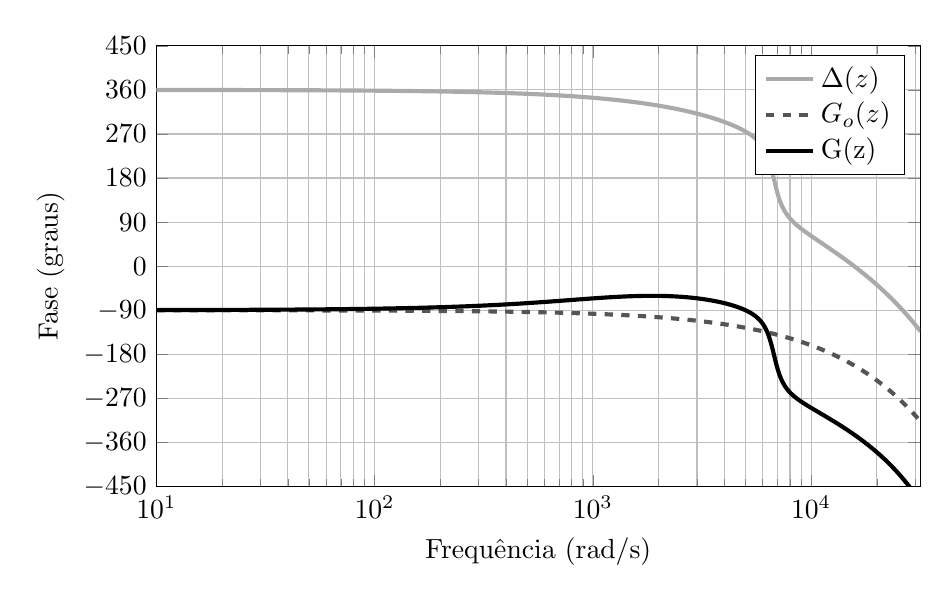
\begin{tikzpicture}

\begin{axis}[%
width=0.8\textwidth,
height=0.461611624834875\textwidth,
scale only axis,
xmode=log,
xmin=10,
xmax=31622.7766016838,
xminorticks=true,
xlabel={Frequência (rad/s)},
xmajorgrids,
xminorgrids,
ymin=-450,
ymax=450,
ytick={-450, -360, -270, -180,  -90,    0,   90,  180,  270,  360,  450},
ylabel={Fase (graus)},
ymajorgrids,
legend style={draw=black,fill=white,legend cell align=left}
]
\addplot [color=mycolor1,solid,line width=1.5pt]
  table[row sep=crcr]{10	359.839042834018\\
10.0461810465159	359.838299516997\\
10.0925753619375	359.83755276726\\
10.139183931163	359.836802568956\\
10.1860077436388	359.836048906157\\
10.2330477933808	359.835291762865\\
10.2803050789954	359.834531123006\\
10.3277806037004	359.833766970433\\
10.375475375347	359.832999288924\\
10.4233904064403	359.832228062181\\
10.4715267141616	359.831453273833\\
10.5198853203895	359.830674907431\\
10.5684672517218	359.829892946452\\
10.6172735394972	359.829107374296\\
10.6663052198171	359.828318174285\\
10.715563333568	359.827525329667\\
10.7650489264432	359.826728823609\\
10.814763048965	359.825928639203\\
10.8647067565072	359.825124759463\\
10.9148811093176	359.824317167322\\
10.9652871725401	359.823505845636\\
11.0159260162376	359.822690777182\\
11.0667987154147	359.821871944656\\
11.1179063500406	359.821049330677\\
11.1692500050717	359.820222917781\\
11.2208307704748	359.819392688424\\
11.2726497412507	359.818558624981\\
11.3247080174565	359.817720709746\\
11.3770067042298	359.816878924931\\
11.4295469118117	359.816033252666\\
11.4823297555707	359.815183674998\\
11.535356356026	359.814330173892\\
11.5886278388715	359.813472731229\\
11.6421453349997	359.812611328807\\
11.6959099805258	359.811745948338\\
11.7499229168114	359.810876571452\\
11.8041852904894	359.810003179693\\
11.8586982534876	359.80912575452\\
11.9134629630538	359.808244277306\\
11.96848058178	359.807358729338\\
12.0237522776272	359.806469091817\\
12.0792792239501	359.805575345858\\
12.135062599522	359.804677472486\\
12.1911035885602	359.803775452642\\
12.2474033807505	359.802869267176\\
12.3039631712731	359.801958896852\\
12.3607841608273	359.801044322342\\
12.4178675556577	359.800125524232\\
12.4752145675793	359.799202483016\\
12.5328264140034	359.7982751791\\
12.5907043179635	359.797343592798\\
12.6488495081411	359.796407704333\\
12.7072632188919	359.795467493838\\
12.765946690272	359.794522941353\\
12.8249011680643	359.793574026826\\
12.8841279038047	359.792620730113\\
12.9436281548089	359.791663030977\\
13.0034031841991	359.790700909086\\
13.0634542609305	359.789734344016\\
13.1237826598188	359.788763315247\\
13.1843896615665	359.787787802167\\
13.2452765527909	359.786807784066\\
13.306444626051	359.785823240139\\
13.3678951798747	359.784834149486\\
13.4296295187868	359.78384049111\\
13.4916489533366	359.782842243915\\
13.5539548001256	359.781839386711\\
13.6165483818355	359.780831898208\\
13.6794310272563	359.779819757018\\
13.7426040713143	359.778802941655\\
13.806068855101	359.777781430532\\
13.8698267259009	359.776755201965\\
13.9338790372205	359.775724234168\\
13.998227148817	359.774688505254\\
14.062872426727	359.773647993236\\
14.1278162432955	359.772602676025\\
14.1930599772055	359.771552531431\\
14.2586050135065	359.77049753716\\
14.3244527436445	359.769437670815\\
14.3906045654914	359.768372909897\\
14.4570618833745	359.767303231803\\
14.5238261081064	359.766228613824\\
14.5908986570152	359.765149033147\\
14.658280953974	359.764064466855\\
14.7259744294318	359.762974891922\\
14.7939805204436	359.761880285219\\
14.8623006707006	359.760780623509\\
14.9309363305612	359.759675883446\\
14.999888957082	359.758566041579\\
15.069160014048	359.757451074347\\
15.1387509720044	359.75633095808\\
15.2086633082875	359.755205669\\
15.2788985070559	359.754075183217\\
15.3494580593225	359.752939476734\\
15.4203434629857	359.751798525441\\
15.4915562228612	359.750652305115\\
15.5630978507143	359.749500791425\\
15.6349698652918	359.748343959926\\
15.7071737923542	359.747181786058\\
15.779711164708	359.74601424515\\
15.8525835222385	359.744841312417\\
15.9257924119422	359.743662962959\\
15.9993393879601	359.742479171761\\
16.07322601161	359.741289913692\\
16.1474538514202	359.740095163506\\
16.2220244831628	359.738894895839\\
16.2969394898867	359.737689085211\\
16.3722004619516	359.736477706025\\
16.4478089970617	359.735260732564\\
16.5237667002994	359.734038138993\\
16.6000751841599	359.732809899358\\
16.6767360685846	359.731575987585\\
16.7537509809962	359.730336377479\\
16.8311215563331	359.729091042725\\
16.9088494370839	359.727839956886\\
16.9869362733223	359.726583093402\\
17.0653837227424	359.725320425593\\
17.1441934506935	359.724051926652\\
17.2233671302159	359.722777569652\\
17.302906442076	359.721497327539\\
17.3828130748022	359.720211173135\\
17.4630887247206	359.718919079137\\
17.5437350959914	359.717621018114\\
17.6247539006444	359.716316962511\\
17.7061468586161	359.715006884644\\
17.7879156977856	359.713690756701\\
17.8700621540116	359.712368550743\\
17.9525879711692	359.711040238701\\
18.035494901187	359.709705792376\\
18.1187847040838	359.70836518344\\
18.2024591480069	359.707018383432\\
18.2865200092687	359.705665363763\\
18.3709690723849	359.704306095708\\
18.4558081301122	359.702940550413\\
18.5410389834868	359.701568698888\\
18.6266634418617	359.70019051201\\
18.7126833229461	359.698805960523\\
18.7991004528435	359.697415015034\\
18.8859166660905	359.696017646014\\
18.9731338056957	359.694613823799\\
19.060753723179	359.693203518588\\
19.1487782786108	359.691786700441\\
19.2372093406515	359.690363339281\\
19.3260487865912	359.688933404892\\
19.4152985023894	359.687496866919\\
19.5049603827153	359.686053694864\\
19.5950363309877	359.684603858091\\
19.6855282594159	359.683147325821\\
19.7764380890397	359.681684067135\\
19.8677677497706	359.680214050969\\
19.9595191804325	359.678737246116\\
20.0516943288031	359.677253621226\\
20.1442951516552	359.675763144802\\
20.2373236147981	359.674265785204\\
20.3307816931193	359.672761510645\\
20.4246713706267	359.67125028919\\
20.5189946404906	359.669732088758\\
20.6137535050858	359.668206877119\\
20.7089499760343	359.666674621896\\
20.8045860742482	359.665135290559\\
20.900663829972	359.663588850432\\
20.9971852828265	359.662035268684\\
21.0941524818514	359.660474512334\\
21.1915674855492	359.658906548251\\
21.2894323619287	359.657331343148\\
21.387749188549	359.655748863584\\
21.4865200525637	359.654159075967\\
21.5857470507649	359.652561946546\\
21.685432289628	359.650957441417\\
21.7855778853565	359.649345526517\\
21.8861859639264	359.647726167628\\
21.987258661132	359.646099330373\\
22.0887981226306	359.644464980215\\
22.1908065039887	359.642823082459\\
22.2932859707273	359.64117360225\\
22.396238698368	359.639516504571\\
22.499666872479	359.637851754245\\
22.603572688722	359.636179315929\\
22.7079583528983	359.634499154121\\
22.8128260809959	359.632811233152\\
22.9181780992365	359.631115517191\\
23.0240166441225	359.629411970238\\
23.130343962485	359.62770055613\\
23.237162311531	359.625981238535\\
23.3444739588916	359.624253980954\\
23.4522811826701	359.62251874672\\
23.5605862714901	359.620775498996\\
23.6693915245447	359.619024200773\\
23.7786992516445	359.617264814876\\
23.8885117732672	359.615497303953\\
23.9988314206069	359.613721630482\\
24.1096605356231	359.611937756769\\
24.2210014710909	359.610145644944\\
24.3328565906507	359.608345256961\\
24.4452282688584	359.606536554602\\
24.558118891236	359.604719499469\\
24.6715308543219	359.602894052988\\
24.7854665657221	359.601060176408\\
24.899928444161	359.599217830798\\
25.0149189195332	359.597366977046\\
25.1304404329547	359.595507575861\\
25.2464954368146	359.59363958777\\
25.3630863948276	359.591762973118\\
25.4802157820863	359.589877692067\\
25.597886085113	359.587983704595\\
25.7160998019135	359.586080970494\\
25.8348594420295	359.584169449371\\
25.9541675265918	359.582249100648\\
26.0740265883745	359.580319883557\\
26.194439171848	359.578381757143\\
26.3154078332332	359.576434680263\\
26.4369351405564	359.574478611582\\
26.5590236737027	359.572513509576\\
26.6816760244719	359.570539332526\\
26.8048947966327	359.568556038525\\
26.9286826059784	359.566563585469\\
27.0530420803822	359.56456193106\\
27.1779758598533	359.562551032806\\
27.3034865965925	359.560530848018\\
27.4295769550488	359.55850133381\\
27.556249611976	359.556462447097\\
27.6835072564894	359.554414144597\\
27.8113525901229	359.552356382826\\
27.9397883268864	359.5502891181\\
28.0688171933232	359.548212306535\\
28.1984419285683	359.546125904041\\
28.3286652844062	359.544029866327\\
28.4594900253294	359.541924148896\\
28.5909189285972	359.539808707047\\
28.7229547842946	359.537683495872\\
28.8556003953913	359.535548470254\\
28.9888585778017	359.53340358487\\
29.1227321604441	359.531248794185\\
29.2572239853012	359.529084052458\\
29.3923369074803	359.526909313732\\
29.5280737952738	359.52472453184\\
29.6644375302202	359.522529660403\\
29.8014310071653	359.520324652826\\
29.9390571343235	359.518109462298\\
30.0773188333397	359.515884041795\\
30.2162190393513	359.513648344073\\
30.3557607010504	359.511402321671\\
30.4959467807464	359.509145926909\\
30.6367802544292	359.506879111886\\
30.7782641118319	359.50460182848\\
30.9204013564946	359.502314028348\\
31.063195005828	359.500015662921\\
31.2066480911777	359.497706683409\\
31.350763657888	359.495387040795\\
31.4955447653674	359.493056685836\\
31.6409944871527	359.49071556906\\
31.7871159109747	359.488363640768\\
31.9339121388238	359.486000851033\\
32.0813862870155	359.483627149695\\
32.229541486257	359.481242486363\\
32.3783808817133	359.478846810413\\
32.5279076330741	359.476440070989\\
32.6781249146208	359.474022216997\\
32.8290359152942	359.471593197111\\
32.9806438387618	359.469152959764\\
33.132951903486	359.466701453154\\
33.2859633427924	359.464238625237\\
33.4396814049384	359.461764423732\\
33.5941093531822	359.459278796114\\
33.7492504658521	359.456781689615\\
33.9051080364161	359.454273051226\\
34.0616853735517	359.45175282769\\
34.2189858012163	359.449220965507\\
34.3770126587175	359.446677410929\\
34.5357693007845	359.444122109958\\
34.6952590976386	359.441555008349\\
34.8554854350656	359.438976051606\\
35.0164517144866	359.436385184979\\
35.1781613530314	359.433782353469\\
35.3406177836102	359.43116750182\\
35.5038244549868	359.428540574522\\
35.6677848318515	359.425901515809\\
35.8325023948954	359.423250269657\\
35.9979806408833	359.420586779782\\
36.1642230827288	359.417910989643\\
36.3312332495683	359.415222842435\\
36.4990146868361	359.412522281093\\
36.6675709563398	359.409809248286\\
36.8369056363357	359.407083686421\\
37.007022321605	359.404345537637\\
37.1779246235299	359.401594743807\\
37.3496161701703	359.398831246534\\
37.5221006063408	359.396054987152\\
37.6953815936883	359.393265906727\\
37.8694628107696	359.390463946047\\
38.0443479531292	359.387649045632\\
38.2200407333782	359.384821145724\\
38.3965448812729	359.381980186291\\
38.5738641437941	359.379126107023\\
38.7520022852263	359.37625884733\\
38.9309630872381	359.373378346345\\
39.1107503489621	359.370484542917\\
39.2913678870758	359.367577375616\\
39.4728195358824	359.364656782725\\
39.6551091473924	359.361722702244\\
39.8382405914052	359.358775071887\\
40.0222177555915	359.355813829077\\
40.2070445455755	359.352838910953\\
40.3927248850181	359.349850254359\\
40.5792627157	359.346847795852\\
40.7666619976054	359.343831471691\\
40.9549267090063	359.340801217844\\
41.1440608465467	359.337756969984\\
41.3340684253274	359.334698663483\\
41.5249534789915	359.331626233418\\
41.7167200598098	359.328539614566\\
41.9093722387671	359.3254387414\\
42.1029141056481	359.322323548094\\
42.2973497691249	359.319193968516\\
42.4926833568435	359.316049936229\\
42.6889190155123	359.312891384488\\
42.8860609109892	359.309718246241\\
43.0841132283705	359.306530454128\\
43.2830801720801	359.303327940474\\
43.4829659659579	359.300110637296\\
43.6837748533501	359.296878476292\\
43.8855110971994	359.293631388849\\
44.0881789801347	359.290369306035\\
44.2917828045629	359.2870921586\\
44.4963268927599	359.283799876974\\
44.701815586962	359.280492391267\\
44.9082532494586	359.277169631264\\
45.1156442626847	359.273831526427\\
45.3239930293136	359.270478005894\\
45.5333039723509	359.267108998472\\
45.7435815352278	359.263724432641\\
45.954830181896	359.260324236553\\
46.167054396922	359.256908338025\\
46.3802586855826	359.253476664541\\
46.5944475739604	359.250029143252\\
46.8096256090399	359.246565700971\\
47.0257973588042	359.243086264174\\
47.2429674123316	359.239590758996\\
47.4611403798933	359.236079111233\\
47.6803208930514	359.232551246336\\
47.9005136047569	359.229007089414\\
48.1217231894485	359.225446565228\\
48.3439543431522	359.221869598194\\
48.5672117835806	359.218276112376\\
48.791500250233	359.21466603149\\
49.0168245044966	359.211039278898\\
49.243189329747	359.207395777609\\
49.4705995314498	359.203735450276\\
49.6990599372628	359.200058219195\\
49.9285753971387	359.196364006303\\
50.1591507834275	359.192652733176\\
50.3907909909802	359.188924321029\\
50.6235009372529	359.185178690713\\
50.8572855624109	359.181415762713\\
51.0921498294339	359.177635457146\\
51.3280987242209	359.173837693762\\
51.5651372556965	359.170022391939\\
51.8032704559168	359.166189470683\\
52.0425033801768	359.162338848626\\
52.2828411071172	359.158470444024\\
52.5242887388322	359.154584174756\\
52.7668514009784	359.150679958322\\
53.010534242883	359.14675771184\\
53.2553424376533	359.142817352046\\
53.5012811822866	359.138858795291\\
53.7483556977805	359.134881957541\\
53.9965712292437	359.130886754371\\
54.2459330460073	359.12687310097\\
54.4964464417369	359.122840912133\\
54.7481167345445	359.11879010226\\
55.0009492671021	359.11472058536\\
55.2549494067543	359.110632275042\\
55.510122545633	359.106525084516\\
55.7664741007712	359.102398926591\\
56.0240095142187	359.098253713676\\
56.282734253157	359.094089357772\\
56.5426538100157	359.089905770475\\
56.8037737025889	359.085702862975\\
57.0660994741527	359.081480546048\\
57.3296366935823	359.07723873006\\
57.5943909554708	359.072977324963\\
57.8603678802477	359.068696240294\\
58.1275731142982	359.06439538517\\
58.3960123300829	359.06007466829\\
58.6656912262587	359.055733997931\\
58.9366155277994	359.051373281947\\
59.2087909861172	359.046992427764\\
59.4822233791852	359.042591342384\\
59.7569185116595	359.038169932377\\
60.0328822150028	359.033728103883\\
60.3101203476082	359.029265762607\\
60.5886387949234	359.024782813821\\
60.8684434695757	359.020279162356\\
61.1495403114975	359.015754712607\\
61.4319352880526	359.011209368526\\
61.7156343941624	359.006643033621\\
62.0006436524339	359.002055610955\\
62.2869691132868	358.997447003144\\
62.5746168550822	358.992817112352\\
62.8635929842521	358.988165840293\\
63.1539036354283	358.983493088228\\
63.445554971573	358.97879875696\\
63.7385531841099	358.974082746835\\
64.032904493055	358.969344957738\\
64.3286151471491	358.964585289093\\
64.6256914239905	358.959803639858\\
64.9241396301678	358.954999908526\\
65.2239661013943	358.95017399312\\
65.5251772026422	358.945325791192\\
65.827779328278	358.940455199822\\
66.1317789021976	358.935562115613\\
66.4371823779638	358.930646434694\\
66.7439962389419	358.925708052709\\
67.0522269984386	358.920746864824\\
67.3618811998395	358.915762765721\\
67.6729654167483	358.910755649593\\
67.9854862531262	358.905725410147\\
68.2994503434323	358.900671940597\\
68.6148643527643	358.895595133666\\
68.931734977	358.89049488158\\
69.2500689429393	358.885371076068\\
69.5698730084476	358.880223608358\\
69.8911539625984	358.875052369177\\
70.213918625818	358.869857248748\\
70.5381738500302	358.864638136784\\
70.8639265188016	358.859394922491\\
71.191183547488	358.854127494565\\
71.5199518833808	358.848835741183\\
71.8502385058548	358.843519550011\\
72.1820504265165	358.838178808193\\
72.5153946893524	358.832813402352\\
72.8502783708792	358.827423218589\\
73.1867085802933	358.822008142478\\
73.5246924596224	358.816568059064\\
73.8642371838769	358.811102852862\\
74.2053499612018	358.805612407855\\
74.5480380330304	358.800096607487\\
74.8923086742377	358.794555334666\\
75.2381691932944	358.78898847176\\
75.585626932423	358.78339590059\\
75.9346892677529	358.777777502437\\
76.2853636094773	358.772133158028\\
76.6376574020103	358.766462747543\\
76.9915781241455	358.760766150607\\
77.3471332892138	358.75504324629\\
77.7043304452438	358.749293913103\\
78.0631771751216	358.743518028996\\
78.4236810967518	358.737715471356\\
78.7858498632195	358.731886117003\\
79.1496911629522	358.726029842188\\
79.5152127198837	358.720146522591\\
79.8824222936175	358.714236033318\\
80.2513276795919	358.708298248899\\
80.6219367092452	358.702333043282\\
80.9942572501823	358.696340289836\\
81.3682972063414	358.690319861343\\
81.7440645181619	358.684271629999\\
82.121567162753	358.678195467409\\
82.5008131540631	358.672091244585\\
82.8818105430498	358.665958831943\\
83.2645674178507	358.659798099303\\
83.6490919039556	358.65360891588\\
84.0353921643786	358.647391150288\\
84.423476399831	358.641144670533\\
84.8133528488963	358.634869344012\\
85.2050297882047	358.628565037509\\
85.5985155326084	358.622231617194\\
85.9938184353586	358.615868948617\\
86.3909468882829	358.60947689671\\
86.7899093219629	358.603055325779\\
87.1907142059136	358.596604099503\\
87.5933700487633	358.590123080934\\
87.9978853984339	358.583612132489\\
88.4042688423224	358.577071115951\\
88.8125290074835	358.570499892465\\
89.2226745608124	358.563898322533\\
89.6347142092288	358.557266266016\\
90.0486566998624	358.550603582123\\
90.4645108202374	358.543910129419\\
90.88228539846	358.53718576581\\
91.3019893034057	358.530430348549\\
91.7236314449071	358.523643734231\\
92.1472207739435	358.516825778785\\
92.5727662828307	358.509976337477\\
93.0002770054119	358.503095264905\\
93.4297620172496	358.496182414995\\
93.8612304358183	358.489237640998\\
94.2946914206979	358.482260795487\\
94.730154173768	358.475251730355\\
95.1676279394036	358.468210296813\\
95.6071220046713	358.46113634538\\
96.0486456995261	358.454029725889\\
96.4922083970099	358.446890287479\\
96.9378195134503	358.439717878589\\
97.3854885086602	358.432512346963\\
97.8352248861393	358.425273539638\\
98.2870381932753	358.418001302946\\
98.7409380215466	358.41069548251\\
99.1969340067261	358.40335592324\\
99.655035829086	358.395982469329\\
100.115253213603	358.388574964251\\
100.577595930163	358.381133250757\\
101.042073793774	358.373657170872\\
101.508696664767	358.366146565891\\
101.977474449012	358.358601276377\\
102.448417098122	358.351021142157\\
102.921534609671	358.343406002316\\
103.3968370274	358.335755695199\\
103.874334441436	358.328070058402\\
104.354036988501	358.320348928774\\
104.83595485213	358.312592142407\\
105.320098262886	358.304799534638\\
105.80647749858	358.296970940044\\
106.295102884484	358.289106192437\\
106.785984793556	358.281205124863\\
107.279133646656	358.273267569595\\
107.774559912768	358.265293358134\\
108.272274109224	358.2572823212\\
108.772286801926	358.249234288734\\
109.27460860557	358.24114908989\\
109.779250183872	358.233026553034\\
110.286222249794	358.224866505739\\
110.795535565772	358.216668774781\\
111.307200943943	358.208433186138\\
111.821229246378	358.200159564982\\
112.337631385307	358.191847735681\\
112.856418323356	358.183497521787\\
113.377601073777	358.175108746043\\
113.901190700682	358.166681230369\\
114.427198319278	358.158214795865\\
114.955635096105	358.149709262803\\
115.486512249268	358.141164450628\\
116.019841048683	358.132580177948\\
116.555632816306	358.123956262535\\
117.093898926384	358.115292521319\\
117.634650805689	358.106588770387\\
118.177899933763	358.097844824972\\
118.723657843162	358.089060499458\\
119.271936119701	358.080235607371\\
119.822746402699	358.071369961373\\
120.376100385228	358.062463373265\\
120.932009814357	358.053515653977\\
121.490486491407	358.044526613565\\
122.051542272196	358.03549606121\\
122.615189067297	358.026423805211\\
123.181438842284	358.01730965298\\
123.750303617991	358.008153411043\\
124.321795470765	357.998954885029\\
124.895926532723	357.989713879673\\
125.472708992008	357.980430198806\\
126.052155093052	357.971103645354\\
126.63427713683	357.961734021331\\
127.219087481126	357.952321127841\\
127.806598540793	357.942864765066\\
128.396822788018	357.933364732266\\
128.989772752585	357.923820827775\\
129.585461022141	357.914232848994\\
130.183900242466	357.904600592391\\
130.785103117737	357.894923853492\\
131.389082410804	357.885202426879\\
131.995850943453	357.875436106187\\
132.605421596686	357.865624684098\\
133.217807310988	357.855767952333\\
133.833021086605	357.845865701657\\
134.451075983821	357.835917721863\\
135.071985123233	357.825923801778\\
135.69576168603	357.815883729252\\
136.322418914273	357.805797291154\\
136.951970111177	357.795664273372\\
137.584428641392	357.785484460802\\
138.219807931287	357.775257637349\\
138.858121469236	357.76498358592\\
139.499382805904	357.754662088418\\
140.143605554534	357.74429292574\\
140.790803391236	357.733875877771\\
141.440990055278	357.72341072338\\
142.094179349378	357.712897240415\\
142.750385139995	357.702335205697\\
143.409621357626	357.691724395018\\
144.0719019971	357.681064583133\\
144.737241117876	357.670355543759\\
145.405652844341	357.659597049566\\
146.077151366109	357.648788872176\\
146.751750938323	357.637930782155\\
147.42946588196	357.627022549011\\
148.110310584131	357.616063941187\\
148.794299498388	357.605054726056\\
149.481447145032	357.593994669917\\
150.171768111418	357.582883537992\\
150.865277052271	357.571721094416\\
151.561988689989	357.560507102237\\
152.261917814963	357.549241323408\\
152.965079285884	357.537923518782\\
153.671488030065	357.52655344811\\
154.381159043753	357.515130870031\\
155.094107392451	357.503655542071\\
155.810348211234	357.492127220636\\
156.529896705074	357.480545661008\\
157.25276814916	357.468910617338\\
157.978977889225	357.457221842642\\
158.708541341869	357.445479088795\\
159.441473994887	357.433682106528\\
160.177791407599	357.421830645419\\
160.917509211179	357.409924453891\\
161.66064310899	357.397963279205\\
162.40720887691	357.385946867455\\
163.157222363676	357.373874963562\\
163.910699491214	357.36174731127\\
164.66765625498	357.34956365314\\
165.428108724297	357.337323730543\\
166.192073042701	357.325027283656\\
166.959565428276	357.312674051459\\
167.730602174008	357.300263771722\\
168.505199648122	357.287796181007\\
169.283374294433	357.275271014661\\
170.065142632699	357.262688006806\\
170.850521258965	357.250046890338\\
171.639526845917	357.237347396919\\
172.432176143241	357.224589256973\\
173.228485977972	357.211772199677\\
174.028473254854	357.19889595296\\
174.832154956701	357.185960243493\\
175.639548144754	357.172964796687\\
176.450669959044	357.159909336683\\
177.265537618758	357.146793586349\\
178.084168422602	357.133617267273\\
178.906579749169	357.120380099758\\
179.732789057308	357.107081802816\\
180.562813886497	357.093722094161\\
181.39667185721	357.080300690202\\
182.234380671297	357.066817306042\\
183.075958112354	357.053271655466\\
183.921422046107	357.039663450938\\
184.770790420785	357.025992403594\\
185.624081267505	357.012258223237\\
186.481312700654	356.99846061833\\
187.342502918271	356.984599295989\\
188.207670202438	356.970673961979\\
189.076832919665	356.956684320705\\
189.950009521279	356.942630075209\\
190.827218543818	356.928510927159\\
191.708478609426	356.914326576848\\
192.593808426241	356.900076723185\\
193.483226788801	356.885761063687\\
194.376752578439	356.871379294476\\
195.274404763682	356.85693111027\\
196.176202400658	356.842416204379\\
197.082164633495	356.827834268695\\
197.992310694735	356.813184993688\\
198.906659905733	356.7984680684\\
199.825231677076	356.783683180435\\
200.748045508988	356.768830015956\\
201.675120991751	356.753908259677\\
202.606477806113	356.738917594856\\
203.542135723711	356.723857703289\\
204.482114607491	356.708728265301\\
205.426434412127	356.693528959744\\
206.375115184445	356.678259463985\\
207.32817706385	356.662919453902\\
208.285640282755	356.647508603875\\
209.247525167004	356.632026586784\\
210.213852136311	356.616473073995\\
211.18464170469	356.600847735358\\
212.159914480891	356.585150239201\\
213.139691168835	356.569380252316\\
214.123992568061	356.55353743996\\
215.112839574156	356.537621465843\\
216.10625317921	356.521631992124\\
217.104254472254	356.505568679399\\
218.106864639713	356.4894311867\\
219.114104965849	356.473219171484\\
220.12599683322	356.456932289625\\
221.142561723131	356.440570195409\\
222.163821216089	356.424132541527\\
223.189796992262	356.407618979064\\
224.220510831939	356.391029157497\\
225.255984615994	356.374362724681\\
226.296240326348	356.357619326849\\
227.341300046436	356.340798608598\\
228.391185961678	356.323900212885\\
229.44592035995	356.306923781018\\
230.505525632052	356.28986895265\\
231.570024272191	356.272735365769\\
232.639438878451	356.255522656692\\
233.713792153278	356.238230460057\\
234.793106903962	356.220858408816\\
235.877406043117	356.203406134225\\
236.966712589169	356.185873265837\\
238.061049666849	356.168259431498\\
239.160440507677	356.150564257331\\
240.264908450462	356.132787367736\\
241.374476941791	356.114928385379\\
242.48916953653	356.096986931182\\
243.609009898327	356.078962624318\\
244.734021800108	356.060855082202\\
245.864229124585	356.042663920482\\
246.999655864764	356.024388753031\\
248.140326124455	356.00602919194\\
249.286264118777	355.98758484751\\
250.437494174681	355.969055328241\\
251.594040731461	355.950440240826\\
252.755928341275	355.931739190142\\
253.923181669665	355.912951779244\\
255.09582549608	355.894077609351\\
256.273884714404	355.875116279843\\
257.457384333485	355.856067388249\\
258.646349477661	355.836930530242\\
259.840805387301	355.817705299625\\
261.040777419332	355.79839128833\\
262.246291047787	355.7789880864\\
263.457371864337	355.75949528199\\
264.674045578839	355.73991246135\\
265.896338019882	355.720239208822\\
267.124275135332	355.700475106828\\
268.357882992886	355.680619735862\\
269.597187780627	355.660672674483\\
270.842215807572	355.640633499301\\
272.092993504239	355.620501784974\\
273.349547423206	355.600277104195\\
274.611904239671	355.579959027686\\
275.880090752022	355.559547124184\\
277.154133882405	355.539040960438\\
278.434060677294	355.518440101195\\
279.719898308069	355.497744109193\\
281.011674071587	355.476952545152\\
282.309415390768	355.456064967763\\
283.613149815172	355.43508093368\\
284.922905021585	355.413999997509\\
286.238708814609	355.392821711802\\
287.560589127251	355.371545627044\\
288.888574021513	355.350171291645\\
290.222691688993	355.328698251929\\
291.562970451479	355.307126052127\\
292.909438761552	355.285454234365\\
294.262125203191	355.263682338656\\
295.621058492378	355.241809902889\\
296.98626747771	355.219836462819\\
298.357781141006	355.197761552058\\
299.735628597932	355.175584702065\\
301.119839098607	355.153305442135\\
302.510442028234	355.130923299393\\
303.907466907719	355.108437798778\\
305.310943394298	355.085848463035\\
306.720901282168	355.063154812708\\
308.137370503119	355.040356366128\\
309.560381127168	355.017452639399\\
310.989963363199	354.994443146394\\
312.426147559604	354.97132739874\\
313.868964204927	354.948104905812\\
315.318443928511	354.924775174716\\
316.774617501149	354.901337710286\\
318.237515835737	354.877792015067\\
319.707169987928	354.854137589311\\
321.183611156796	354.830373930959\\
322.666870685493	354.806500535637\\
324.156980061919	354.782516896642\\
325.653970919389	354.75842250493\\
327.1578750373	354.734216849109\\
328.668724341813	354.709899415426\\
330.186550906528	354.685469687754\\
331.711386953162	354.660927147586\\
333.243264852235	354.636271274019\\
334.78221712376	354.611501543748\\
336.328276437929	354.586617431048\\
337.881475615808	354.561618407771\\
339.441847630035	354.536503943328\\
341.009425605519	354.511273504682\\
342.584242820144	354.485926556335\\
344.166332705473	354.460462560315\\
345.75572884746	354.43488097617\\
347.352464987164	354.409181260949\\
348.956575021463	354.383362869197\\
350.568093003772	354.357425252939\\
352.187053144771	354.331367861674\\
353.813489813129	354.305190142353\\
355.447437536229	354.278891539381\\
357.088931000911	354.252471494592\\
358.738005054198	354.225929447248\\
360.39469470404	354.199264834018\\
362.059035120061	354.172477088973\\
363.731061634299	354.145565643572\\
365.410809741959	354.118529926645\\
367.09831510217	354.09136936439\\
368.793613538734	354.064083380354\\
370.496741040893	354.036671395422\\
372.207733764093	354.009132827805\\
373.926628030746	353.981467093031\\
375.653460331008	353.953673603927\\
377.388267323548	353.925751770609\\
379.13108583633	353.897701000472\\
380.881952867393	353.869520698172\\
382.640905585636	353.84121026562\\
384.407981331609	353.812769101963\\
386.183217618305	353.784196603575\\
387.966652131954	353.755492164042\\
389.758322732826	353.726655174154\\
391.558267456034	353.697685021883\\
393.366524512341	353.66858109238\\
395.183132288971	353.639342767956\\
397.008129350424	353.609969428068\\
398.841554439296	353.580460449311\\
400.683446477099	353.5508152054\\
402.533844565089	353.521033067159\\
404.392787985098	353.491113402509\\
406.260316200361	353.461055576449\\
408.136468856361	353.430858951049\\
410.021285781671	353.400522885433\\
411.914806988789	353.370046735766\\
413.817072675003	353.339429855241\\
415.72812322323	353.308671594064\\
417.647999202884	353.27777129944\\
419.576741370729	353.246728315562\\
421.514390671752	353.215541983593\\
423.460988240025	353.184211641656\\
425.416575399583	353.152736624818\\
427.381193665299	353.121116265073\\
429.354884743766	353.089349891334\\
431.337690534184	353.057436829414\\
433.329653129246	353.025376402013\\
435.330814816033	352.993167928704\\
437.341218076915	352.960810725918\\
439.360905590448	352.92830410693\\
441.389920232282	352.895647381844\\
443.428305076071	352.862839857579\\
445.476103394389	352.829880837853\\
447.533358659646	352.796769623168\\
449.600114545014	352.763505510798\\
451.67641492535	352.730087794772\\
453.762303878129	352.696515765857\\
455.857825684385	352.662788711546\\
457.963024829641	352.628905916044\\
460.077946004862	352.594866660247\\
462.202634107401	352.560670221734\\
464.33713424195	352.526315874744\\
466.481491721497	352.491802890168\\
468.635752068297	352.457130535528\\
470.799961014824	352.422298074964\\
472.974164504755	352.387304769218\\
475.158408693936	352.352149875618\\
477.352739951367	352.316832648061\\
479.557204860185	352.281352337001\\
481.771850218653	352.245708189427\\
483.996723041153	352.209899448854\\
486.231870559183	352.173925355299\\
488.477340222363	352.137785145273\\
490.73317969944	352.101478051758\\
492.999436879299	352.065003304196\\
495.276159871982	352.028360128467\\
497.563397009708	351.991547746878\\
499.861196847899	351.954565378144\\
502.169608166212	351.917412237369\\
504.48867996957	351.880087536033\\
506.818461489212	351.842590481975\\
509.159002183727	351.804920279373\\
511.51035174011	351.76707612873\\
513.872560074817	351.729057226855\\
516.245677334823	351.690862766847\\
518.629753898685	351.652491938079\\
521.024840377617	351.613943926176\\
523.430987616559	351.575217913005\\
525.848246695256	351.53631307665\\
528.27666892935	351.4972285914\\
530.716305871459	351.457963627728\\
533.167209312278	351.418517352274\\
535.629431281677	351.378888927829\\
538.103024049808	351.339077513316\\
540.588040128206	351.299082263771\\
543.084532270915	351.258902330327\\
545.592553475602	351.218536860192\\
548.11215698468	351.177984996636\\
550.643396286443	351.13724587897\\
553.186325116201	351.096318642526\\
555.740997457415	351.055202418642\\
558.307467542852	351.013896334641\\
560.885789855729	350.972399513813\\
563.476019130871	350.930711075396\\
566.078210355879	350.888830134558\\
568.692418772287	350.846755802376\\
571.318699876742	350.804487185819\\
573.957109422183	350.762023387731\\
576.607703419019	350.719363506804\\
579.27053813632	350.676506637568\\
581.945670103016	350.633451870365\\
584.633156109091	350.590198291333\\
587.333053206791	350.546744982384\\
590.045418711838	350.503091021186\\
592.77031020464	350.459235481144\\
595.507785531519	350.415177431376\\
598.25790280594	350.3709159367\\
601.020720409738	350.326450057606\\
603.796296994364	350.28177885024\\
606.584691482126	350.236901366386\\
609.385963067442	350.19181665344\\
612.200171218097	350.146523754393\\
615.027375676503	350.101021707812\\
617.867636460969	350.055309547815\\
620.721013866976	350.009386304052\\
623.587568468455	349.963251001687\\
626.467361119072	349.916902661371\\
629.360452953524	349.870340299227\\
632.266905388836	349.823562926826\\
635.186780125658	349.776569551165\\
638.120139149584	349.729359174646\\
641.067044732464	349.681930795056\\
644.027559433723	349.634283405544\\
647.001746101695	349.586415994599\\
649.989667874954	349.53832754603\\
652.991388183652	349.490017038941\\
656.00697075087	349.441483447711\\
659.03647959397	349.392725741973\\
662.07997902595	349.343742886589\\
665.137533656814	349.294533841627\\
668.209208394941	349.245097562344\\
671.295068448464	349.195432999157\\
674.395179326655	349.145539097623\\
677.509606841313	349.095414798417\\
680.638417108163	349.045059037306\\
683.78167654826	348.99447074513\\
686.9394518894	348.943648847775\\
690.11181016753	348.892592266153\\
693.298818728181	348.841299916175\\
696.500545227891	348.789770708729\\
699.717057635642	348.73800354966\\
702.948424234306	348.685997339737\\
706.19471362209	348.63375097464\\
709.455994713995	348.581263344927\\
712.732336743282	348.528533336015\\
716.023809262934	348.475559828154\\
719.330482147139	348.422341696402\\
722.652425592773	348.3688778106\\
725.989710120886	348.315167035352\\
729.3424065782	348.261208229991\\
732.71058613862	348.207000248564\\
736.094320304735	348.1525419398\\
739.493680909343	348.097832147086\\
742.908740116972	348.042869708445\\
746.339570425412	347.987653456507\\
749.786244667258	347.932182218484\\
753.248836011454	347.876454816145\\
756.727417964843	347.820470065789\\
760.222064373731	347.76422677822\\
763.732849425456	347.707723758719\\
767.259847649959	347.650959807022\\
770.803133921369	347.593933717287\\
774.362783459591	347.536644278072\\
777.938871831903	347.479090272306\\
781.531474954562	347.421270477266\\
785.140669094413	347.363183664542\\
788.76653087051	347.304828600017\\
792.40913725574	347.246204043838\\
796.068565578463	347.187308750386\\
799.744893524145	347.128141468249\\
803.438199137013	347.068700940196\\
807.148560821713	347.008985903148\\
810.876057344967	346.94899508815\\
814.620767837254	346.888727220339\\
818.382771794484	346.828181018922\\
822.162149079689	346.767355197143\\
825.958979924714	346.706248462254\\
829.773344931927	346.644859515488\\
833.605325075921	346.583187052028\\
837.455001705243	346.52122976098\\
841.322456544116	346.45898632534\\
845.207771694168	346.396455421967\\
849.111029636188	346.333635721552\\
853.032313231867	346.270525888587\\
856.971705725559	346.207124581338\\
860.92929074605	346.143430451811\\
864.905152308334	346.079442145723\\
868.899374815392	346.015158302471\\
872.91204305999	345.9505775551\\
876.943242226474	345.885698530274\\
880.993057892579	345.820519848243\\
885.061576031251	345.75504012281\\
889.148883012464	345.689257961305\\
893.255065605058	345.623171964544\\
897.380210978585	345.556780726804\\
901.52440670515	345.49008283579\\
905.687740761275	345.423076872597\\
909.870301529772	345.355761411685\\
914.07217780161	345.288135020838\\
918.293458777803	345.220196261138\\
922.534234071309	345.151943686926\\
926.794593708924	345.083375845772\\
931.074628133199	345.014491278438\\
935.374428204358	344.945288518848\\
939.694085202226	344.875766094049\\
944.033690828168	344.80592252418\\
948.39333720704	344.735756322435\\
952.773116889131	344.665265995029\\
957.173122852146	344.594450041164\\
961.593448503166	344.52330695299\\
966.034187680636	344.451835215572\\
970.495434656357	344.380033306853\\
974.977284137491	344.30789969762\\
979.479831268559	344.235432851463\\
984.003171633478	344.162631224742\\
988.547401257578	344.089493266549\\
993.112616609642	344.016017418669\\
997.698914603958	343.942202115546\\
1002.30639260238	343.868045784241\\
1006.93514841637	343.793546844397\\
1011.58528030912	343.7187037082\\
1016.2568869976	343.643514780339\\
1020.95006765465	343.567978457969\\
1025.66492191112	343.492093130669\\
1030.40154985798	343.415857180407\\
1035.16005204838	343.339268981494\\
1039.94052949988	343.26232690055\\
1044.74308369654	343.185029296459\\
1049.56781659108	343.107374520331\\
1054.41483060703	343.029360915459\\
1059.28422864096	342.950986817281\\
1064.17611406461	342.872250553332\\
1069.09059072708	342.793150443208\\
1074.02776295708	342.713684798522\\
1078.98773556513	342.633851922859\\
1083.97061384575	342.553650111736\\
1088.97650357974	342.473077652556\\
1094.00551103639	342.392132824566\\
1099.05774297578	342.310813898811\\
1104.13330665098	342.229119138093\\
1109.2323098104	342.147046796922\\
1114.35486070002	342.064595121472\\
1119.50106806574	341.981762349538\\
1124.67104115564	341.898546710486\\
1129.86488972231	341.814946425208\\
1135.0827240252	341.730959706077\\
1140.32465483296	341.646584756897\\
1145.59079342577	341.561819772857\\
1150.8812515977	341.476662940482\\
1156.19614165913	341.391112437585\\
1161.53557643908	341.305166433217\\
1166.89966928762	341.21882308762\\
1172.28853407829	341.132080552173\\
1177.70228521052	341.044936969346\\
1183.14103761204	340.957390472647\\
1188.60490674132	340.869439186569\\
1194.09400859005	340.781081226542\\
1199.60845968555	340.692314698878\\
1205.14837709331	340.603137700719\\
1210.71387841942	340.513548319982\\
1216.30508181309	340.42354463531\\
1221.92210596917	340.33312471601\\
1227.56507013062	340.242286622006\\
1233.23409409112	340.151028403776\\
1238.92929819754	340.059348102303\\
1244.65080335254	339.967243749014\\
1250.3987310171	339.874713365723\\
1256.17320321316	339.781754964573\\
1261.97434252612	339.688366547981\\
1267.80227210752	339.594546108574\\
1273.65711567764	339.500291629134\\
1279.53899752808	339.405601082532\\
1285.44804252445	339.310472431673\\
1291.38437610901	339.214903629431\\
1297.34812430331	339.118892618586\\
1303.33941371088	339.022437331762\\
1309.35837151994	338.925535691366\\
1315.40512550606	338.828185609518\\
1321.47980403488	338.730384987988\\
1327.58253606487	338.632131718134\\
1333.71345115004	338.533423680827\\
1339.87267944269	338.434258746393\\
1346.06035169616	338.334634774536\\
1352.27659926764	338.234549614275\\
1358.52155412096	338.134001103868\\
1364.79534882933	338.03298707075\\
1371.09811657822	337.931505331451\\
1377.42999116818	337.82955369153\\
1383.79110701763	337.727129945501\\
1390.18159916578	337.624231876754\\
1396.60160327544	337.520857257486\\
1403.05125563594	337.417003848619\\
1409.53069316601	337.312669399726\\
1416.04005341668	337.207851648951\\
1422.5794745742	337.102548322931\\
1429.14909546299	336.996757136714\\
1435.74905554856	336.890475793677\\
1442.3794949405	336.783701985445\\
1449.04055439544	336.676433391808\\
1455.73237532004	336.568667680633\\
1462.45509977397	336.46040250778\\
1469.20887047298	336.351635517015\\
1475.99383079187	336.242364339917\\
1482.81012476756	336.132586595798\\
1489.65789710218	336.0222998916\\
1496.53729316606	335.911501821813\\
1503.44845900091	335.800189968372\\
1510.39154132284	335.688361900571\\
1517.36668752555	335.576015174958\\
1524.37404568338	335.463147335245\\
1531.41376455451	335.349755912202\\
1538.4859935841	335.235838423559\\
1545.59088290748	335.121392373904\\
1552.72858335329	335.006415254577\\
1559.89924644673	334.890904543569\\
1567.10302441275	334.774857705406\\
1574.34007017931	334.65827219105\\
1581.61053738059	334.541145437781\\
1588.91458036027	334.423474869088\\
1596.25235417481	334.305257894554\\
1603.62401459674	334.18649190974\\
1611.02971811795	334.067174296066\\
1618.46962195303	333.947302420691\\
1625.94388404263	333.826873636394\\
1633.45266305675	333.705885281446\\
1640.99611839816	333.584334679486\\
1648.57441020578	333.462219139393\\
1656.18769935804	333.339535955155\\
1663.83614747635	333.216282405735\\
1671.51991692849	333.092455754939\\
1679.23917083208	332.968053251276\\
1686.99407305804	332.843072127821\\
1694.78478823403	332.717509602069\\
1702.61148174801	332.591362875793\\
1710.47431975172	332.464629134898\\
1718.37346916419	332.337305549266\\
1726.30909767531	332.209389272609\\
1734.28137374936	332.080877442308\\
1742.29046662864	331.951767179261\\
1750.33654633699	331.822055587714\\
1758.41978368348	331.691739755104\\
1766.54035026596	331.560816751885\\
1774.69841847474	331.429283631364\\
1782.89416149627	331.297137429521\\
1791.12775331676	331.164375164835\\
1799.39936872594	331.030993838102\\
1807.70918332073	330.896990432253\\
1816.05737350894	330.762361912164\\
1824.44411651309	330.627105224465\\
1832.86959037413	330.491217297343\\
1841.33397395519	330.354695040348\\
1849.83744694544	330.217535344184\\
1858.38018986386	330.079735080504\\
1866.9623840631	329.9412911017\\
1875.58421173328	329.802200240684\\
1884.24585590593	329.662459310669\\
1892.94750045783	329.522065104947\\
1901.68933011491	329.381014396653\\
1910.47153045619	329.239303938536\\
1919.29428791772	329.096930462719\\
1928.15778979652	328.953890680452\\
1937.06222425457	328.810181281865\\
1946.00778032282	328.66579893571\\
1954.99464790516	328.520740289104\\
1964.02301778248	328.37500196726\\
1973.09308161673	328.228580573216\\
1982.20503195496	328.081472687559\\
1991.35906223344	327.933674868137\\
2000.55536678172	327.78518364977\\
2009.79414082682	327.635995543955\\
2019.07558049731	327.48610703856\\
2028.39988282751	327.335514597515\\
2037.76724576168	327.184214660494\\
2047.17786815819	327.032203642589\\
2056.63194979376	326.879477933982\\
2066.12969136771	326.726033899597\\
2075.6712945062	326.571867878761\\
2085.25696176653	326.416976184844\\
2094.88689664142	326.261355104894\\
2104.56130356336	326.105000899265\\
2114.2803879089	325.947909801236\\
2124.04435600306	325.79007801662\\
2133.8534151237	325.631501723365\\
2143.70777350589	325.472177071139\\
2153.60764034637	325.312100180918\\
2163.55322580795	325.151267144551\\
2173.54474102401	324.98967402432\\
2183.58239810298	324.827316852491\\
2193.66641013278	324.66419163085\\
2203.79699118545	324.500294330231\\
2213.97435632161	324.335620890027\\
2224.19872159503	324.170167217697\\
2234.47030405729	324.003929188249\\
2244.78932176229	323.836902643725\\
2255.15599377096	323.669083392659\\
2265.57054015585	323.500467209528\\
2276.03318200585	323.331049834188\\
2286.54414143084	323.160826971296\\
2297.10364156645	322.989794289715\\
2307.71190657875	322.817947421905\\
2318.36916166905	322.645281963298\\
2329.07563307865	322.471793471657\\
2339.83154809368	322.297477466416\\
2350.63713504986	322.122329428004\\
2361.49262333744	321.946344797155\\
2372.39824340596	321.769518974188\\
2383.35422676926	321.591847318282\\
2394.36080601029	321.413325146722\\
2405.4182147861	321.233947734126\\
2416.52668783283	321.053710311654\\
2427.6864609706	320.87260806619\\
2438.8977711086	320.690636139511\\
2450.16085625011	320.50778962742\\
2461.4759554975	320.324063578867\\
2472.84330905736	320.139452995035\\
2484.26315824557	319.953952828413\\
2495.73574549243	319.767557981827\\
2507.26131434783	319.580263307461\\
2518.84010948637	319.392063605833\\
2530.4723767126	319.202953624755\\
2542.15836296621	319.012928058257\\
2553.8983163273	318.821981545484\\
2565.69248602162	318.630108669551\\
2577.54112242586	318.437303956381\\
2589.444477073	318.243561873495\\
2601.4028026576	318.04887682877\\
2613.41635304121	317.853243169168\\
2625.48538325773	317.656655179416\\
2637.61014951883	317.459107080656\\
2649.7909092194	317.260593029047\\
2662.02792094301	317.061107114332\\
2674.32144446738	316.860643358357\\
2686.67174076992	316.659195713546\\
2699.07907203326	316.456758061333\\
2711.54370165082	316.253324210541\\
2724.0658942324	316.048887895715\\
2736.64591560979	315.8434427754\\
2749.28403284242	315.636982430369\\
2761.98051422303	315.429500361795\\
2774.73562928336	315.220989989366\\
2787.54964879989	315.011444649335\\
2800.42284479955	314.800857592521\\
2813.35549056553	314.58922198223\\
2826.34786064309	314.376530892128\\
2839.40023084533	314.162777304027\\
2852.51287825912	313.947954105615\\
2865.68608125093	313.732054088105\\
2878.92011947275	313.515069943809\\
2892.21527386804	313.29699426363\\
2905.57182667769	313.077819534479\\
2918.99006144599	312.857538136598\\
2932.4702630267	312.636142340799\\
2946.01271758903	312.413624305615\\
2959.61771262377	312.18997607434\\
2973.28553694936	311.965189571993\\
2987.01648071805	311.739256602154\\
3000.81083542203	311.512168843714\\
3014.66889389963	311.2839178475\\
3028.59095034155	311.054495032789\\
3042.57730029708	310.823891683701\\
3056.6282406804	310.592098945469\\
3070.74406977686	310.359107820574\\
3084.92508724934	310.124909164747\\
3099.17159414457	309.889493682834\\
3113.48389289956	309.652851924505\\
3127.86228734801	309.414974279821\\
3142.30708272674	309.175850974633\\
3156.8185856822	308.935472065819\\
3171.39710427697	308.693827436351\\
3186.04294799627	308.450906790179\\
3200.75642775457	308.206699646925\\
3215.53785590219	307.961195336392\\
3230.38754623189	307.714382992856\\
3245.30581398558	307.466251549155\\
3260.29297586097	307.216789730555\\
3275.34935001834	306.965986048384\\
3290.47525608724	306.713828793422\\
3305.67101517332	306.460306029045\\
3320.93694986511	306.205405584105\\
3336.27338424092	305.949115045529\\
3351.68064387565	305.691421750641\\
3367.15905584778	305.432312779179\\
3382.70894874623	305.171774945002\\
3398.3306526774	304.909794787463\\
3414.02449927217	304.64635856245\\
3429.7908216929	304.381452233062\\
3445.62995464054	304.115061459913\\
3461.54223436172	303.847171591042\\
3477.5279986559	303.577767651418\\
3493.58758688252	303.306834332009\\
3509.72133996824	303.034355978405\\
3525.92960041413	302.760316578968\\
3542.21271230298	302.484699752491\\
3558.57102130658	302.207488735336\\
3575.00487469309	301.928666368025\\
3591.51462133436	301.648215081272\\
3608.1006117134	301.366116881408\\
3624.76319793175	301.082353335182\\
3641.50273371703	300.796905553899\\
3658.31957443038	300.509754176876\\
3675.21407707406	300.220879354157\\
3692.18660029898	299.930260728475\\
3709.23750441235	299.637877416405\\
3726.36715138533	299.343707988673\\
3743.57590486067	299.047730449575\\
3760.86413016048	298.749922215464\\
3778.23219429398	298.450260092245\\
3795.68046596523	298.148720251838\\
3813.20931558105	297.845278207546\\
3830.81911525882	297.539908788273\\
3848.51023883439	297.232586111519\\
3866.28306187004	296.923283555103\\
3884.13796166242	296.61197372753\\
3902.07531725059	296.29862843693\\
3920.09550942403	295.983218658489\\
3938.19892073078	295.665714500291\\
3956.38593548549	295.346085167473\\
3974.65693977764	295.024298924605\\
3993.0123214797	294.700323056184\\
4011.45247025537	294.374123825136\\
4029.97777756789	294.045666429218\\
4048.58863668828	293.714914955176\\
4067.28544270374	293.381832330545\\
4086.06859252603	293.046380272937\\
4104.93848489988	292.708519236671\\
4123.89552041149	292.368208356586\\
4142.94010149697	292.025405388848\\
4162.07263245094	291.680066648588\\
4181.29351943512	291.33214694415\\
4200.60317048688	290.981599507759\\
4220.00199552799	290.628375922354\\
4239.49040637325	290.272426044368\\
4259.06881673929	289.913697922173\\
4278.73764225331	289.55213770992\\
4298.49730046193	289.187689576459\\
4318.34821084004	288.820295609032\\
4338.2907947997	288.449895711368\\
4358.32547569911	288.07642749582\\
4378.45267885158	287.69982616913\\
4398.67283153454	287.320024411385\\
4418.98636299868	286.936952247701\\
4439.39370447695	286.550536912117\\
4459.89528919383	286.160702703157\\
4480.49155237446	285.767370830467\\
4501.18293125388	285.370459251891\\
4521.96986508636	284.969882500279\\
4542.85279515466	284.565551499305\\
4563.83216477945	284.15737336746\\
4584.90841932869	283.745251209355\\
4606.0820062271	283.32908389338\\
4627.35337496566	282.908765814689\\
4648.72297711113	282.484186642378\\
4670.19126631568	282.055231049662\\
4691.75869832646	281.621778425701\\
4713.42573099534	281.183702567656\\
4735.19282428857	280.7408713514\\
4757.06044029659	280.29314637917\\
4779.02904324381	279.840382602319\\
4801.09909949849	279.382427917117\\
4823.27107758263	278.9191227314\\
4845.54544818189	278.450299499648\\
4867.92268415562	277.975782223833\\
4890.4032605469	277.495385917165\\
4912.98765459258	277.008916027564\\
4935.67634573345	276.516167817376\\
4958.46981562442	276.016925695565\\
4981.36854814472	275.510962498188\\
5004.37302940819	274.998038712599\\
5027.48374777359	274.477901640356\\
5050.70119385497	273.950284493326\\
5074.02586053209	273.414905416929\\
5097.4582429609	272.871466433857\\
5120.998838584	272.319652300944\\
5144.64814714125	271.759129271117\\
5168.40667068035	271.189543751567\\
5192.27491356753	270.610520848338\\
5216.2533824982	270.021662786589\\
5240.34258650778	269.422547194656\\
5264.54303698246	268.812725238851\\
5288.85524767004	268.191719594616\\
5313.27973469088	267.559022238178\\
5337.81701654885	266.914092041291\\
5362.46761414231	266.256352149875\\
5387.23205077517	265.585187125509\\
5412.11085216805	264.899939826665\\
5437.10454646936	264.199908004382\\
5462.21366426659	263.484340584711\\
5487.43873859752	262.752433607799\\
5512.78030496154	262.003325790847\\
5538.23890133107	261.236093679529\\
5563.81506816292	260.449746349785\\
5589.50934840979	259.64321961928\\
5615.32228753178	258.815369725462\\
5641.254433508	257.964966425175\\
5667.30633684818	257.090685469423\\
5693.47855060436	256.191100406567\\
5719.77163038263	255.264673668349\\
5746.18613435493	254.309746896323\\
5772.72262327089	253.324530472409\\
5799.38166046975	252.307092227382\\
5826.16381189231	251.25534531667\\
5853.06964609293	250.16703527573\\
5880.09973425162	249.03972629986\\
5907.25465018618	247.870786838856\\
5934.53497036433	246.657374659211\\
5961.94127391598	245.396421610757\\
5989.47414264556	244.084618446902\\
6017.13416104428	242.718400195454\\
6044.92191630263	241.293932769532\\
6072.83799832281	239.807101755628\\
6100.88299973121	238.253504629887\\
6129.05751589107	236.628448045742\\
6157.36214491506	234.92695231636\\
6185.79748767801	233.143765789759\\
6214.36414782964	231.273392480051\\
6243.06273180741	229.310137056258\\
6271.89384884933	227.248172056128\\
6300.85811100697	225.081632902534\\
6329.95613315842	222.804746815664\\
6359.18853302131	220.412001823307\\
6388.55593116599	217.898361477132\\
6418.05895102864	215.259529201821\\
6447.69821892457	212.492262996335\\
6477.47436406142	209.594736051148\\
6507.38801855264	206.566931482028\\
6537.43981743082	203.411049928639\\
6567.63039866118	200.131897988736\\
6597.96040315515	196.737215002165\\
6628.43047478397	193.237888151474\\
6659.0412603923	189.648004434694\\
6689.79340981204	185.984695853585\\
6720.68757587607	182.267752802502\\
6751.7244144321	178.519009084355\\
6782.90458435663	174.761535763985\\
6814.22874756894	171.018712913744\\
6845.69756904508	167.313270129185\\
6877.31171683206	163.666392446267\\
6909.07186206199	160.096976321434\\
6940.97867896634	156.621094056355\\
6973.03284489025	153.251691564298\\
7005.23504030693	149.998511787019\\
7037.58594883204	146.86821081086\\
7070.0862572383	143.864619025027\\
7102.73665547	140.989095469165\\
7135.53783665763	138.240927512619\\
7168.49049713269	135.617736947984\\
7201.59533644237	133.115864403778\\
7234.85305736446	130.730714422831\\
7268.26436592224	128.457052304652\\
7301.82997139948	126.289250370109\\
7335.55058635552	124.22148572161\\
7369.42692664033	122.24789418041\\
7403.45971140979	120.362686325408\\
7437.64966314091	118.560231860155\\
7471.99750764715	116.835118250355\\
7506.50397409388	115.18218896858\\
7541.16979501382	113.596565939999\\
7575.99570632259	112.073660019753\\
7610.98244733438	110.609172616994\\
7646.13076077758	109.199090946636\\
7681.44139281058	107.839678849358\\
7716.91509303763	106.527464672763\\
7752.55261452471	105.259227343768\\
7788.35471381553	104.031981473505\\
7824.32215094763	102.842962109427\\
7860.45568946846	101.68960957398\\
7896.7560964516	100.569554695064\\
7933.22414251308	99.4806046321141\\
7969.86060182773	98.4207294259527\\
8006.66625214554	97.3880493447533\\
8043.6418748083	96.3808230580096\\
8080.78825476606	95.3974366415777\\
8118.10618059391	94.4363933968539\\
8155.5964445086	93.4963044537411\\
8193.25984238547	92.5758801185131\\
8231.09717377527	91.6739219227399\\
8269.10924192116	90.7893153270585\\
8307.29685377578	89.9210230330434\\
8345.66082001834	89.0680788571726\\
8384.20195507185	88.2295821224897\\
8422.92107712042	87.4046925256998\\
8461.81900812665	86.5926254399307\\
8500.89657384898	85.792647616013\\
8540.15460385935	85.0040732478223\\
8579.59393156072	84.2262603698823\\
8619.21539420481	83.4586075579829\\
8659.01983290983	82.7005509060166\\
8699.0080926784	81.9515612545356\\
8739.18102241541	81.211141648674\\
8779.5394749461	80.4788250050718\\
8820.08430703417	79.7541719692734\\
8860.81637939989	79.0367689467554\\
8901.73655673847	78.3262262922743\\
8942.84570773836	77.622176643642\\
8984.14470509972	76.9242733873043\\
9025.63442555289	76.2321892442673\\
9067.31574987707	75.5456149659713\\
9109.18956291901	74.8642581306683\\
9151.25675361173	74.1878420317274\\
9193.51821499347	73.516104650073\\
9235.97484422661	72.8487977036811\\
9278.62754261669	72.1856857676926\\
9321.47721563161	71.5265454592881\\
9364.5247729208	70.8711646819989\\
9407.77112833455	70.2193419245997\\
9451.21719994339	69.5708856101634\\
9494.86391005764	68.9256134912497\\
9538.71218524688	68.2833520875524\\
9582.76295635973	67.6439361626482\\
9627.01715854358	67.0072082367852\\
9671.47573126437	66.3730181329127\\
9716.13961832666	65.7412225533863\\
9761.00976789355	65.1116846850096\\
9806.08713250686	64.4842738302655\\
9851.37266910737	63.8588650627675\\
9896.86733905512	63.2353389051313\\
9942.57210814977	62.6135810276093\\
9988.48794665118	61.9934819659691\\
10034.6158293	61.3749368572197\\
10080.9567353382	60.7578451919006\\
10127.5116485301	60.1421105817535\\
10174.2815571832	59.527640541686\\
10221.267454169	58.914346285029\\
10268.4703369442	58.30214253116\\
10315.891207572	57.6909473246408\\
10363.531072743	57.0806818650825\\
10411.3909437969	56.4712703470108\\
10459.4718367439	55.8626398090577\\
10507.7747722864	55.2547199918608\\
10556.3007758401	54.6474432040911\\
10605.0508775566	54.0407441960788\\
10654.0261123446	53.4345600405414\\
10703.2275198921	52.8288300199574\\
10752.6561446888	52.2234955201579\\
10802.3130360475	51.618499929746\\
10852.1992481272	51.0137885449732\\
10902.315839955	50.4093084797326\\
10952.6638754485	49.8050085803549\\
11003.244423439	49.2008393449081\\
11054.0585576935	48.5967528467289\\
11105.1073569377	47.9927026619303\\
11156.3919048792	47.388643800646\\
11207.9132902301	46.7845326417867\\
11259.6726067303	46.1803268711065\\
11311.6709531708	45.5759854223789\\
11363.9094334169	44.9714684215091\\
11416.3891564316	44.3667371334035\\
11469.1112362992	43.7617539114495\\
11522.0767922492	43.1564821494474\\
11575.2869486794	42.5508862358627\\
11628.7428351806	41.9449315102654\\
11682.4455865599	41.3385842218377\\
11736.3963428651	40.7318114898316\\
11790.596249409	40.1245812658758\\
11845.0464567934	39.5168622980255\\
11899.7481209338	38.908624096465\\
11954.7024030838	38.299836900772\\
12009.9104698599	37.6904716486647\\
12065.3734932659	37.0804999461473\\
12121.0926507183	36.4698940389865\\
12177.069125071	35.8586267854475\\
12233.3041046402	35.2466716302223\\
12289.7987832301	34.6340025794928\\
12346.554360158	34.0205941770703\\
12403.5720402798	33.4064214815541\\
12460.8530340153	32.791460044462\\
12518.3985573745	32.1756858892811\\
12576.2098319827	31.5590754913963\\
12634.2880851072	30.9416057588496\\
12692.6345496825	30.3232540138939\\
12751.2504643373	29.7039979753004\\
12810.1370734203	29.0838157413836\\
12869.2956270265	28.462685773709\\
12928.7273810244	27.8405868814543\\
12988.4335970818	27.2174982063874\\
13048.4155426933	26.5933992084395\\
13108.6744912069	25.9682696518402\\
13169.2117218509	25.3420895917911\\
13230.0285197614	24.7148393616517\\
13291.1261760091	24.0864995606169\\
13352.5059876274	23.4570510418605\\
13414.1692576393	22.8264749011261\\
13476.1172950852	22.1947524657467\\
13538.351415051	21.5618652840686\\
13600.8729386957	20.9277951152681\\
13663.6831932795	20.2925239195402\\
13726.7835121922	19.6560338486431\\
13790.1752349813	19.0183072367859\\
13853.8597073802	18.3793265918421\\
13917.8382813373	17.739074586875\\
13982.1123150444	17.0975340519647\\
14046.6831729655	16.4546879663196\\
14111.552225866	15.8105194506647\\
14176.7208508414	15.165011759893\\
14242.190431347	14.5181482759702\\
14307.9623572268	13.8699125010805\\
14374.0380247435	13.2202880510061\\
14440.4188366077	12.5692586487284\\
14507.1062020079	11.9168081182465\\
14574.1015366405	11.2629203785962\\
14641.4062627396	10.6075794380725\\
14709.0218091073	9.95076938863729\\
14776.9496111443	9.29247440051096\\
14845.1911108798	8.63267871693837\\
14913.7477570027	7.97136664912576\\
14982.6210048919	7.30852257133512\\
15051.8123166476	6.64413091613959\\
15121.323161122	5.97817616982411\\
15191.1550139505	5.31064286793301\\
15261.3093575835	4.64151559095431\\
15331.7876813171	3.97077896014059\\
15402.5914813253	3.2984176334541\\
15473.7222606918	2.62441630164082\\
15545.1815294413	1.94875968441958\\
15616.9708045722	1.27143252678836\\
15689.0916100885	0.592419595440165\\
15761.5454770323	-0.0882943247132895\\
15834.333943516	-0.770724433914605\\
15907.4585547554	-1.45488592083656\\
15980.9208631021	-2.14079396576028\\
16054.7224280766	-2.8284637436615\\
16128.8648164017	-3.51791042720891\\
16203.3496020352	-4.20914918967549\\
16278.1783662036	-4.90219520776591\\
16353.352697436	-5.59706366436651\\
16428.8741915971	-6.29376975121612\\
16504.7444519217	-6.99232867150269\\
16580.9650890484	-7.69275564238869\\
16657.537721054	-8.39506589746644\\
16734.4639734876	-9.09927468914458\\
16811.7454794054	-9.8053972909735\\
16889.3838794052	-10.5134489999047\\
16967.3808216612	-11.2234451384916\\
17045.7379619589	-11.9354010570312\\
17124.4569637308	-12.6493321356502\\
17203.539498091	-13.365253786334\\
17282.9872438709	-14.0831814549064\\
17362.8018876552	-14.8031306229567\\
17442.9851238172	-15.5251168097173\\
17523.5386545551	-16.2491555738955\\
17604.464189928	-16.9752625154582\\
17685.7634478922	-17.7034532773706\\
17767.4381543379	-18.4337435472965\\
17849.4900431252	-19.1661490592533\\
17931.9208561219	-19.9006855952301\\
18014.7323432394	-20.6373689867636\\
18097.9262624709	-21.3762151164819\\
18181.5043799277	-22.1172399196071\\
18265.4684698776	-22.8604593854273\\
18349.8203147818	-23.605889558733\\
18434.5617053333	-24.3535465412235\\
18519.6944404947	-25.1034464928787\\
18605.2203275364	-25.8556056333054\\
18691.1411820748	-26.6100402430508\\
18777.4588281113	-27.3667666648907\\
18864.1750980704	-28.1258013050904\\
18951.2918328392	-28.8871606346409\\
19038.810881806	-29.6508611904666\\
19126.7341029	-30.4169195766159\\
19215.0633626303	-31.1853524654217\\
19303.8005361259	-31.9561765986457\\
19392.9475071751	-32.7294087885986\\
19482.506168266	-33.505065919243\\
19572.4784206263	-34.2831649472726\\
19662.8661742637	-35.0637229031793\\
19753.6713480067	-35.8467568922962\\
19844.8958695449	-36.6322840958294\\
19936.5416754703	-37.4203217718704\\
20028.6107113184	-38.2108872563956\\
20121.1049316092	-39.003997964251\\
20214.026299889	-39.7996713901207\\
20307.3767887718	-40.5979251094873\\
20401.1583799817	-41.3987767795768\\
20495.373064394	-42.2022441402935\\
20590.0228420787	-43.0083450151441\\
20685.1097223421	-43.8170973121528\\
20780.6357237695	-44.6285190247645\\
20876.6028742684	-45.4426282327429\\
20973.0132111115	-46.2594431030594\\
21069.8687809795	-47.078981890774\\
21167.1716400053	-47.9012629399125\\
21264.923853817	-48.7263046843347\\
21363.127497582	-49.5541256485997\\
21461.7846560511	-50.3847444488262\\
21560.8974236026	-51.2181797935494\\
21660.467904287	-52.0544504845745\\
21760.4982118713	-52.8935754178283\\
21860.9904698845	-53.735573584209\\
21961.9468116618	-54.5804640704339\\
22063.3693803907	-55.4282660598876\\
22165.260329156	-56.2789988334711\\
22267.6218209858	-57.1326817704522\\
22370.4560288971	-57.989334349313\\
22473.7651359423	-58.8489761486074\\
22577.5513352553	-59.7116268478134\\
22681.8168300982	-60.5773062281953\\
22786.5638339077	-61.4460341736664\\
22891.7945703429	-62.3178306716587\\
22997.5112733313	-63.1927158139958\\
23103.7161871177	-64.0707097977764\\
23210.4115663104	-64.9518329262586\\
23317.5996759301	-65.8361056097575\\
23425.2827914574	-66.7235483665477\\
23533.4631988815	-67.6141818237782\\
23642.1431947482	-68.5080267183916\\
23751.3250862094	-69.4051038980605\\
23861.0111910714	-70.3054343221292\\
23971.2038378446	-71.2090390625716\\
24081.9053657923	-72.1159393049593\\
24193.1181249812	-73.0261563494458\\
24304.8444763306	-73.9397116117605\\
24417.0867916629	-74.8566266242239\\
24529.8474537537	-75.776923036773\\
24643.1288563827	-76.7006226180064\\
24756.933404384	-77.627747256247\\
24871.2635136979	-78.5583189606224\\
24986.1216114214	-79.4923598621639\\
25101.5101358603	-80.4298922149267\\
25217.4315365806	-81.3709383971311\\
25333.8882744609	-82.3155209123246\\
25450.882821744	-83.2636623905682\\
25568.4176620901	-84.2153855896472\\
25686.4952906292	-85.1707133963044\\
25805.1182140139	-86.1296688274997\\
25924.2889504728	-87.0922750317002\\
26044.0100298642	-88.0585552901927\\
26164.2839937291	-89.0285330184306\\
26285.113395346	-90.0022317674074\\
26406.5007997846	-90.9796752250637\\
26528.4487839603	-91.9608872177242\\
26650.959936689	-92.945891711572\\
26774.0368587419	-93.934712814155\\
26897.6821629011	-94.9273747759302\\
27021.8984740145	-95.923901991846\\
27146.6884290521	-96.9243190029622\\
27272.0546771616	-97.9286504981099\\
27397.9998797246	-98.9369213155962\\
27524.5267104134	-99.94915644495\\
27651.6378552475	-100.965381028714\\
27779.3360126509	-101.985620364283\\
27907.623893509	-103.009899905788\\
28036.5042212264	-104.038245266034\\
28165.9797317848	-105.070682218491\\
28296.0531738006	-106.107236699328\\
28426.7273085842	-107.147934809521\\
28558.0049101974	-108.192802816997\\
28689.8887655133	-109.241867158855\\
28822.3816742749	-110.295154443638\\
28955.4864491548	-111.352691453676\\
29089.2059158146	-112.414505147486\\
29223.5429129655	-113.480622662255\\
29358.5002924277	-114.551071316373\\
29494.0809191919	-115.625878612063\\
29630.2876714792	-116.705072238066\\
29767.1234408028	-117.78868007242\\
29904.5911320291	-118.876730185309\\
30042.6936634399	-119.969250842009\\
30181.4339667932	-121.066270505906\\
30320.8149873869	-122.167817841621\\
30460.8396841202	-123.273921718218\\
30601.5110295567	-124.384611212509\\
30742.8320099879	-125.499915612471\\
30884.8056254962	-126.619864420755\\
31027.4348900188	-127.744487358313\\
31170.7228314113	-128.873814368128\\
31314.6724915125	-130.007875619073\\
31459.2869262085	-131.146701509882\\
31604.5692054981	-132.290322673249\\
31750.5224135574	-133.438769980059\\
};
\addlegendentry{$\Delta\text{(z)}$};

\addplot [color=black!50!mycolor1,dashed,line width=1.5pt]
  table[row sep=crcr]{10	-90.0716197243914\\
10.0461810465159	-90.0719504717737\\
10.0925753619375	-90.0722827465821\\
10.139183931163	-90.0726165558703\\
10.1860077436388	-90.0729519067248\\
10.2330477933808	-90.0732888062645\\
10.2803050789954	-90.0736272616417\\
10.3277806037004	-90.0739672800411\\
10.375475375347	-90.0743088686812\\
10.4233904064403	-90.0746520348133\\
10.4715267141616	-90.0749967857225\\
10.5198853203895	-90.0753431287275\\
10.5684672517218	-90.0756910711807\\
10.6172735394972	-90.0760406204686\\
10.6663052198171	-90.0763917840117\\
10.715563333568	-90.0767445692648\\
10.7650489264432	-90.0770989837171\\
10.814763048965	-90.0774550348925\\
10.8647067565072	-90.0778127303494\\
10.9148811093176	-90.0781720776814\\
10.9652871725401	-90.0785330845169\\
11.0159260162376	-90.0788957585198\\
11.0667987154147	-90.0792601073893\\
11.1179063500406	-90.0796261388599\\
11.1692500050717	-90.0799938607021\\
11.2208307704748	-90.0803632807223\\
11.2726497412507	-90.0807344067629\\
11.3247080174565	-90.0811072467023\\
11.3770067042298	-90.0814818084556\\
11.4295469118117	-90.0818580999742\\
11.4823297555707	-90.0822361292465\\
11.535356356026	-90.0826159042975\\
11.5886278388715	-90.0829974331894\\
11.6421453349997	-90.0833807240217\\
11.6959099805258	-90.0837657849311\\
11.7499229168114	-90.0841526240922\\
11.8041852904894	-90.0845412497169\\
11.8586982534876	-90.0849316700555\\
11.9134629630538	-90.0853238933961\\
11.96848058178	-90.085717928065\\
12.0237522776272	-90.0861137824273\\
12.0792792239501	-90.0865114648866\\
12.135062599522	-90.086910983885\\
12.1911035885602	-90.0873123479039\\
12.2474033807505	-90.0877155654639\\
12.3039631712731	-90.0881206451248\\
12.3607841608273	-90.088527595486\\
12.4178675556577	-90.0889364251865\\
12.4752145675793	-90.0893471429053\\
12.5328264140034	-90.0897597573615\\
12.5907043179635	-90.0901742773146\\
12.6488495081411	-90.0905907115641\\
12.7072632188919	-90.0910090689505\\
12.765946690272	-90.0914293583552\\
12.8249011680643	-90.0918515887003\\
12.8841279038047	-90.0922757689493\\
12.9436281548089	-90.0927019081071\\
13.0034031841991	-90.0931300152202\\
13.0634542609305	-90.0935600993767\\
13.1237826598188	-90.0939921697068\\
13.1843896615665	-90.094426235383\\
13.2452765527909	-90.0948623056198\\
13.306444626051	-90.0953003896747\\
13.3678951798747	-90.0957404968475\\
13.4296295187868	-90.0961826364814\\
13.4916489533366	-90.0966268179623\\
13.5539548001256	-90.0970730507198\\
13.6165483818355	-90.0975213442269\\
13.6794310272563	-90.0979717080003\\
13.7426040713143	-90.0984241516007\\
13.806068855101	-90.0988786846331\\
13.8698267259009	-90.0993353167465\\
13.9338790372205	-90.0997940576348\\
13.998227148817	-90.1002549170366\\
14.062872426727	-90.1007179047353\\
14.1278162432955	-90.1011830305597\\
14.1930599772055	-90.1016503043837\\
14.2586050135065	-90.1021197361273\\
14.3244527436445	-90.1025913357557\\
14.3906045654914	-90.1030651132806\\
14.4570618833745	-90.1035410787596\\
14.5238261081064	-90.1040192422971\\
14.5908986570152	-90.1044996140438\\
14.658280953974	-90.1049822041975\\
14.7259744294318	-90.105467023003\\
14.7939805204436	-90.1059540807525\\
14.8623006707006	-90.1064433877857\\
14.9309363305612	-90.10693495449\\
14.999888957082	-90.1074287913007\\
15.069160014048	-90.1079249087015\\
15.1387509720044	-90.1084233172244\\
15.2086633082875	-90.10892402745\\
15.2788985070559	-90.1094270500079\\
15.3494580593225	-90.1099323955765\\
15.4203434629857	-90.1104400748839\\
15.4915562228612	-90.1109500987074\\
15.5630978507143	-90.1114624778744\\
15.6349698652918	-90.1119772232619\\
15.7071737923542	-90.1124943457975\\
15.779711164708	-90.1130138564591\\
15.8525835222385	-90.1135357662753\\
15.9257924119422	-90.1140600863257\\
15.9993393879601	-90.1145868277409\\
16.07322601161	-90.1151160017031\\
16.1474538514202	-90.1156476194461\\
16.2220244831628	-90.1161816922554\\
16.2969394898867	-90.1167182314688\\
16.3722004619516	-90.1172572484765\\
16.4478089970617	-90.1177987547211\\
16.5237667002994	-90.1183427616982\\
16.6000751841599	-90.1188892809565\\
16.6767360685846	-90.1194383240979\\
16.7537509809962	-90.119989902778\\
16.8311215563331	-90.1205440287062\\
16.9088494370839	-90.1211007136459\\
16.9869362733223	-90.1216599694149\\
17.0653837227424	-90.1222218078856\\
17.1441934506935	-90.1227862409851\\
17.2233671302159	-90.1233532806957\\
17.302906442076	-90.1239229390551\\
17.3828130748022	-90.1244952281564\\
17.4630887247206	-90.1250701601486\\
17.5437350959914	-90.125647747237\\
17.6247539006444	-90.126228001683\\
17.7061468586161	-90.1268109358047\\
17.7879156977856	-90.1273965619772\\
17.8700621540116	-90.1279848926327\\
17.9525879711692	-90.1285759402607\\
18.035494901187	-90.1291697174085\\
18.1187847040838	-90.1297662366813\\
18.2024591480069	-90.1303655107425\\
18.2865200092687	-90.1309675523141\\
18.3709690723849	-90.1315723741766\\
18.4558081301122	-90.1321799891698\\
18.5410389834868	-90.1327904101927\\
18.6266634418617	-90.1334036502037\\
18.7126833229461	-90.1340197222212\\
18.7991004528435	-90.1346386393238\\
18.8859166660905	-90.1352604146503\\
18.9731338056957	-90.1358850614004\\
19.060753723179	-90.1365125928346\\
19.1487782786108	-90.1371430222745\\
19.2372093406515	-90.1377763631036\\
19.3260487865912	-90.1384126287669\\
19.4152985023894	-90.1390518327717\\
19.5049603827153	-90.1396939886874\\
19.5950363309877	-90.1403391101464\\
19.6855282594159	-90.1409872108437\\
19.7764380890397	-90.141638304538\\
19.8677677497706	-90.142292405051\\
19.9595191804325	-90.1429495262687\\
20.0516943288031	-90.1436096821408\\
20.1442951516552	-90.144272886682\\
20.2373236147981	-90.1449391539711\\
20.3307816931193	-90.1456084981522\\
20.4246713706267	-90.1462809334348\\
20.5189946404906	-90.146956474094\\
20.6137535050858	-90.1476351344705\\
20.7089499760343	-90.1483169289718\\
20.8045860742482	-90.1490018720714\\
20.900663829972	-90.1496899783099\\
20.9971852828265	-90.150381262295\\
21.0941524818514	-90.1510757387019\\
21.1915674855492	-90.1517734222736\\
21.2894323619287	-90.152474327821\\
21.387749188549	-90.1531784702235\\
21.4865200525637	-90.1538858644294\\
21.5857470507649	-90.1545965254557\\
21.685432289628	-90.155310468389\\
21.7855778853565	-90.1560277083856\\
21.8861859639264	-90.1567482606714\\
21.987258661132	-90.1574721405432\\
22.0887981226306	-90.1581993633679\\
22.1908065039887	-90.1589299445837\\
22.2932859707273	-90.1596638997001\\
22.396238698368	-90.160401244298\\
22.499666872479	-90.1611419940304\\
22.603572688722	-90.1618861646226\\
22.7079583528983	-90.1626337718725\\
22.8128260809959	-90.1633848316509\\
22.9181780992365	-90.1641393599019\\
23.0240166441225	-90.1648973726434\\
23.130343962485	-90.165658885967\\
23.237162311531	-90.1664239160389\\
23.3444739588916	-90.1671924790997\\
23.4522811826701	-90.1679645914651\\
23.5605862714901	-90.1687402695263\\
23.6693915245447	-90.1695195297499\\
23.7786992516445	-90.1703023886788\\
23.8885117732672	-90.1710888629321\\
23.9988314206069	-90.1718789692058\\
24.1096605356231	-90.172672724273\\
24.2210014710909	-90.1734701449842\\
24.3328565906507	-90.1742712482677\\
24.4452282688584	-90.1750760511299\\
24.558118891236	-90.175884570656\\
24.6715308543219	-90.1766968240099\\
24.7854665657221	-90.1775128284348\\
24.899928444161	-90.1783326012535\\
25.0149189195332	-90.1791561598689\\
25.1304404329547	-90.1799835217642\\
25.2464954368146	-90.1808147045032\\
25.3630863948276	-90.1816497257312\\
25.4802157820863	-90.1824886031745\\
25.597886085113	-90.1833313546417\\
25.7160998019135	-90.1841779980234\\
25.8348594420295	-90.1850285512928\\
25.9541675265918	-90.1858830325062\\
26.0740265883745	-90.1867414598032\\
26.194439171848	-90.1876038514074\\
26.3154078332332	-90.1884702256262\\
26.4369351405564	-90.1893406008519\\
26.5590236737027	-90.1902149955614\\
26.6816760244719	-90.1910934283172\\
26.8048947966327	-90.1919759177674\\
26.9286826059784	-90.1928624826462\\
27.0530420803822	-90.1937531417745\\
27.1779758598533	-90.1946479140598\\
27.3034865965925	-90.1955468184971\\
27.4295769550488	-90.1964498741692\\
27.556249611976	-90.1973571002469\\
27.6835072564894	-90.1982685159896\\
27.8113525901229	-90.1991841407455\\
27.9397883268864	-90.2001039939524\\
28.0688171933232	-90.2010280951377\\
28.1984419285683	-90.201956463919\\
28.3286652844062	-90.2028891200044\\
28.4594900253294	-90.2038260831932\\
28.5909189285972	-90.2047673733762\\
28.7229547842946	-90.2057130105356\\
28.8556003953913	-90.2066630147465\\
28.9888585778017	-90.2076174061762\\
29.1227321604441	-90.2085762050854\\
29.2572239853012	-90.2095394318283\\
29.3923369074803	-90.2105071068532\\
29.5280737952738	-90.2114792507025\\
29.6644375302202	-90.2124558840139\\
29.8014310071653	-90.2134370275201\\
29.9390571343235	-90.2144227020497\\
30.0773188333397	-90.2154129285275\\
30.2162190393513	-90.2164077279747\\
30.3557607010504	-90.2174071215099\\
30.4959467807464	-90.218411130349\\
30.6367802544292	-90.2194197758061\\
30.7782641118319	-90.2204330792934\\
30.9204013564946	-90.2214510623222\\
31.063195005828	-90.2224737465032\\
31.2066480911777	-90.2235011535468\\
31.350763657888	-90.2245333052636\\
31.4955447653674	-90.2255702235651\\
31.6409944871527	-90.2266119304638\\
31.7871159109747	-90.227658448074\\
31.9339121388238	-90.228709798612\\
32.0813862870155	-90.2297660043969\\
32.229541486257	-90.2308270878505\\
32.3783808817133	-90.2318930714987\\
32.5279076330741	-90.2329639779708\\
32.6781249146208	-90.2340398300011\\
32.8290359152942	-90.2351206504287\\
32.9806438387618	-90.2362064621982\\
33.132951903486	-90.23729728836\\
33.2859633427924	-90.2383931520711\\
33.4396814049384	-90.2394940765956\\
33.5941093531822	-90.2406000853048\\
33.7492504658521	-90.2417112016779\\
33.9051080364161	-90.2428274493027\\
34.0616853735517	-90.2439488518759\\
34.2189858012163	-90.2450754332035\\
34.3770126587175	-90.2462072172015\\
34.5357693007845	-90.2473442278966\\
34.6952590976386	-90.2484864894259\\
34.8554854350656	-90.2496340260386\\
35.0164517144866	-90.2507868620955\\
35.1781613530314	-90.2519450220699\\
35.3406177836102	-90.2531085305482\\
35.5038244549868	-90.2542774122305\\
35.6677848318515	-90.2554516919307\\
35.8325023948954	-90.2566313945775\\
35.9979806408833	-90.2578165452145\\
36.1642230827288	-90.2590071690012\\
36.3312332495683	-90.2602032912132\\
36.4990146868361	-90.2614049372427\\
36.6675709563398	-90.2626121325993\\
36.8369056363357	-90.2638249029105\\
37.007022321605	-90.2650432739218\\
37.1779246235299	-90.266267271498\\
37.3496161701703	-90.267496921623\\
37.5221006063408	-90.2687322504011\\
37.6953815936883	-90.2699732840567\\
37.8694628107696	-90.2712200489356\\
38.0443479531292	-90.2724725715052\\
38.2200407333782	-90.2737308783551\\
38.3965448812729	-90.2749949961977\\
38.5738641437941	-90.2762649518688\\
38.7520022852263	-90.2775407723281\\
38.9309630872381	-90.2788224846598\\
39.1107503489621	-90.2801101160732\\
39.2913678870758	-90.2814036939032\\
39.4728195358824	-90.2827032456109\\
39.6551091473924	-90.2840087987845\\
39.8382405914052	-90.2853203811393\\
40.0222177555915	-90.2866380205186\\
40.2070445455755	-90.2879617448945\\
40.3927248850181	-90.2892915823681\\
40.5792627157	-90.2906275611703\\
40.7666619976054	-90.2919697096624\\
40.9549267090063	-90.2933180563367\\
41.1440608465467	-90.2946726298171\\
41.3340684253274	-90.2960334588595\\
41.5249534789915	-90.2974005723529\\
41.7167200598098	-90.2987739993195\\
41.9093722387671	-90.3001537689155\\
42.1029141056481	-90.3015399104319\\
42.2973497691249	-90.3029324532949\\
42.4926833568435	-90.3043314270666\\
42.6889190155123	-90.3057368614456\\
42.8860609109892	-90.3071487862676\\
43.0841132283705	-90.3085672315062\\
43.2830801720801	-90.3099922272733\\
43.4829659659579	-90.31142380382\\
43.6837748533501	-90.3128619915371\\
43.8855110971994	-90.3143068209555\\
44.0881789801347	-90.3157583227474\\
44.2917828045629	-90.3172165277265\\
44.4963268927599	-90.3186814668487\\
44.701815586962	-90.3201531712131\\
44.9082532494586	-90.3216316720623\\
45.1156442626847	-90.3231170007832\\
45.3239930293136	-90.3246091889075\\
45.5333039723509	-90.3261082681127\\
45.7435815352278	-90.3276142702226\\
45.954830181896	-90.3291272272079\\
46.167054396922	-90.3306471711868\\
46.3802586855826	-90.3321741344261\\
46.5944475739604	-90.3337081493414\\
46.8096256090399	-90.3352492484982\\
47.0257973588042	-90.3367974646121\\
47.2429674123316	-90.3383528305501\\
47.4611403798933	-90.3399153793307\\
47.6803208930514	-90.3414851441252\\
47.9005136047569	-90.3430621582577\\
48.1217231894485	-90.3446464552065\\
48.3439543431522	-90.3462380686045\\
48.5672117835806	-90.3478370322396\\
48.791500250233	-90.3494433800562\\
49.0168245044966	-90.3510571461551\\
49.243189329747	-90.3526783647948\\
49.4705995314498	-90.3543070703917\\
49.6990599372628	-90.3559432975216\\
49.9285753971387	-90.3575870809196\\
50.1591507834275	-90.3592384554813\\
50.3907909909802	-90.3608974562636\\
50.6235009372529	-90.3625641184851\\
50.8572855624109	-90.3642384775272\\
51.0921498294339	-90.3659205689346\\
51.3280987242209	-90.3676104284161\\
51.5651372556965	-90.3693080918455\\
51.8032704559168	-90.3710135952623\\
52.0425033801768	-90.3727269748724\\
52.2828411071172	-90.3744482670489\\
52.5242887388322	-90.3761775083327\\
52.7668514009784	-90.3779147354337\\
53.010534242883	-90.3796599852314\\
53.2553424376533	-90.3814132947752\\
53.5012811822866	-90.383174701286\\
53.7483556977805	-90.3849442421563\\
53.9965712292437	-90.3867219549516\\
54.2459330460073	-90.3885078774107\\
54.4964464417369	-90.3903020474465\\
54.7481167345445	-90.3921045031474\\
55.0009492671021	-90.3939152827773\\
55.2549494067543	-90.395734424777\\
55.510122545633	-90.3975619677648\\
55.7664741007712	-90.3993979505375\\
56.0240095142187	-90.4012424120707\\
56.282734253157	-90.4030953915203\\
56.5426538100157	-90.4049569282229\\
56.8037737025889	-90.4068270616968\\
57.0660994741527	-90.4087058316428\\
57.3296366935823	-90.4105932779451\\
57.5943909554708	-90.4124894406719\\
57.8603678802477	-90.4143943600766\\
58.1275731142982	-90.4163080765984\\
58.3960123300829	-90.4182306308634\\
58.6656912262587	-90.4201620636853\\
58.9366155277994	-90.422102416066\\
59.2087909861172	-90.4240517291971\\
59.4822233791852	-90.4260100444602\\
59.7569185116595	-90.4279774034282\\
60.0328822150028	-90.4299538478657\\
60.3101203476082	-90.4319394197305\\
60.5886387949234	-90.433934161174\\
60.8684434695757	-90.4359381145422\\
61.1495403114975	-90.4379513223767\\
61.4319352880526	-90.4399738274158\\
61.7156343941624	-90.4420056725947\\
62.0006436524339	-90.4440469010474\\
62.2869691132868	-90.4460975561066\\
62.5746168550822	-90.4481576813055\\
62.8635929842521	-90.4502273203782\\
63.1539036354283	-90.4523065172607\\
63.445554971573	-90.454395316092\\
63.7385531841099	-90.456493761215\\
64.032904493055	-90.458601897177\\
64.3286151471491	-90.4607197687316\\
64.6256914239905	-90.4628474208387\\
64.9241396301678	-90.4649848986658\\
65.2239661013943	-90.4671322475893\\
65.5251772026422	-90.4692895131948\\
65.827779328278	-90.4714567412786\\
66.1317789021976	-90.4736339778485\\
66.4371823779638	-90.4758212691248\\
66.7439962389419	-90.4780186615411\\
67.0522269984386	-90.4802262017455\\
67.3618811998395	-90.4824439366016\\
67.6729654167483	-90.4846719131893\\
67.9854862531262	-90.4869101788061\\
68.2994503434323	-90.4891587809677\\
68.6148643527643	-90.4914177674095\\
68.931734977	-90.493687186087\\
69.2500689429393	-90.4959670851775\\
69.5698730084476	-90.4982575130806\\
69.8911539625984	-90.5005585184195\\
70.213918625818	-90.5028701500418\\
70.5381738500302	-90.5051924570209\\
70.8639265188016	-90.5075254886566\\
71.191183547488	-90.5098692944765\\
71.5199518833808	-90.512223924237\\
71.8502385058548	-90.5145894279242\\
72.1820504265165	-90.516965855755\\
72.5153946893524	-90.5193532581782\\
72.8502783708792	-90.5217516858756\\
73.1867085802933	-90.5241611897631\\
73.5246924596224	-90.5265818209917\\
73.8642371838769	-90.5290136309487\\
74.2053499612018	-90.5314566712585\\
74.5480380330304	-90.5339109937842\\
74.8923086742377	-90.5363766506281\\
75.2381691932944	-90.5388536941334\\
75.585626932423	-90.5413421768848\\
75.9346892677529	-90.5438421517099\\
76.2853636094773	-90.5463536716805\\
76.6376574020103	-90.5488767901131\\
76.9915781241455	-90.5514115605707\\
77.3471332892138	-90.5539580368635\\
77.7043304452438	-90.5565162730503\\
78.0631771751216	-90.5590863234396\\
78.4236810967518	-90.5616682425905\\
78.7858498632195	-90.5642620853142\\
79.1496911629522	-90.5668679066751\\
79.5152127198837	-90.5694857619918\\
79.8824222936175	-90.5721157068383\\
80.2513276795919	-90.5747577970453\\
80.6219367092452	-90.5774120887013\\
80.9942572501823	-90.580078638154\\
81.3682972063414	-90.5827575020112\\
81.7440645181619	-90.585448737142\\
82.121567162753	-90.5881524006782\\
82.5008131540631	-90.5908685500156\\
82.8818105430498	-90.593597242815\\
83.2645674178507	-90.5963385370032\\
83.6490919039556	-90.5990924907748\\
84.0353921643786	-90.6018591625932\\
84.423476399831	-90.6046386111916\\
84.8133528488963	-90.6074308955745\\
85.2050297882047	-90.6102360750188\\
85.5985155326084	-90.6130542090754\\
85.9938184353586	-90.6158853575701\\
86.3909468882829	-90.6187295806047\\
86.7899093219629	-90.6215869385589\\
87.1907142059136	-90.6244574920913\\
87.5933700487633	-90.6273413021402\\
87.9978853984339	-90.6302384299258\\
88.4042688423224	-90.6331489369506\\
88.8125290074835	-90.6360728850015\\
89.2226745608124	-90.6390103361505\\
89.6347142092288	-90.6419613527563\\
90.0486566998624	-90.6449259974656\\
90.4645108202374	-90.6479043332144\\
90.88228539846	-90.6508964232294\\
91.3019893034057	-90.6539023310292\\
91.7236314449071	-90.6569221204258\\
92.1472207739435	-90.6599558555259\\
92.5727662828307	-90.6630036007321\\
93.0002770054119	-90.6660654207447\\
93.4297620172496	-90.6691413805625\\
93.8612304358183	-90.6722315454847\\
94.2946914206979	-90.6753359811118\\
94.730154173768	-90.6784547533476\\
95.1676279394036	-90.6815879283999\\
95.6071220046713	-90.6847355727825\\
96.0486456995261	-90.6878977533163\\
96.4922083970099	-90.6910745371307\\
96.9378195134503	-90.6942659916652\\
97.3854885086602	-90.6974721846707\\
97.8352248861393	-90.7006931842111\\
98.2870381932753	-90.7039290586645\\
98.7409380215466	-90.7071798767247\\
99.1969340067261	-90.7104457074029\\
99.655035829086	-90.713726620029\\
100.115253213603	-90.7170226842529\\
100.577595930163	-90.7203339700463\\
101.042073793774	-90.7236605477041\\
101.508696664767	-90.7270024878456\\
101.977474449012	-90.7303598614164\\
102.448417098122	-90.7337327396898\\
102.921534609671	-90.737121194268\\
103.3968370274	-90.740525297084\\
103.874334441436	-90.7439451204031\\
104.354036988501	-90.7473807368241\\
104.83595485213	-90.7508322192814\\
105.320098262886	-90.7542996410458\\
105.80647749858	-90.7577830757268\\
106.295102884484	-90.7612825972737\\
106.785984793556	-90.7647982799774\\
107.279133646656	-90.7683301984717\\
107.774559912768	-90.7718784277352\\
108.272274109224	-90.7754430430928\\
108.772286801926	-90.7790241202171\\
109.27460860557	-90.7826217351304\\
109.779250183872	-90.7862359642058\\
110.286222249794	-90.7898668841694\\
110.795535565772	-90.7935145721013\\
111.307200943943	-90.7971791054378\\
111.821229246378	-90.8008605619728\\
112.337631385307	-90.8045590198593\\
112.856418323356	-90.8082745576114\\
113.377601073777	-90.8120072541057\\
113.901190700682	-90.815757188583\\
114.427198319278	-90.8195244406501\\
114.955635096105	-90.8233090902816\\
115.486512249268	-90.8271112178211\\
116.019841048683	-90.8309309039835\\
116.555632816306	-90.8347682298564\\
117.093898926384	-90.8386232769016\\
117.634650805689	-90.8424961269577\\
118.177899933763	-90.8463868622405\\
118.723657843162	-90.8502955653461\\
119.271936119701	-90.8542223192516\\
119.822746402699	-90.8581672073176\\
120.376100385228	-90.8621303132896\\
120.932009814357	-90.8661117212997\\
121.490486491407	-90.8701115158686\\
122.051542272196	-90.8741297819074\\
122.615189067297	-90.8781666047194\\
123.181438842284	-90.8822220700015\\
123.750303617991	-90.8862962638467\\
124.321795470765	-90.8903892727454\\
124.895926532723	-90.8945011835876\\
125.472708992008	-90.8986320836644\\
126.052155093052	-90.90278206067\\
126.63427713683	-90.9069512027038\\
127.219087481126	-90.9111395982718\\
127.806598540793	-90.9153473362888\\
128.396822788018	-90.9195745060803\\
128.989772752585	-90.9238211973843\\
129.585461022141	-90.9280875003532\\
130.183900242466	-90.9323735055557\\
130.785103117737	-90.9366793039787\\
131.389082410804	-90.9410049870295\\
131.995850943453	-90.9453506465372\\
132.605421596686	-90.9497163747554\\
133.217807310988	-90.9541022643633\\
133.833021086605	-90.9585084084685\\
134.451075983821	-90.9629349006082\\
135.071985123233	-90.9673818347519\\
135.69576168603	-90.9718493053028\\
136.322418914273	-90.9763374071003\\
136.951970111177	-90.9808462354215\\
137.584428641392	-90.9853758859838\\
138.219807931287	-90.9899264549465\\
138.858121469236	-90.9944980389128\\
139.499382805904	-90.9990907349323\\
140.143605554534	-91.0037046405026\\
140.790803391236	-91.0083398535717\\
141.440990055278	-91.0129964725399\\
142.094179349378	-91.0176745962618\\
142.750385139995	-91.0223743240486\\
143.409621357626	-91.0270957556701\\
144.0719019971	-91.031838991357\\
144.737241117876	-91.0366041318027\\
145.405652844341	-91.0413912781656\\
146.077151366109	-91.0462005320715\\
146.751750938323	-91.0510319956151\\
147.42946588196	-91.055885771363\\
148.110310584131	-91.0607619623553\\
148.794299498388	-91.0656606721079\\
149.481447145032	-91.0705820046148\\
150.171768111418	-91.0755260643502\\
150.865277052271	-91.0804929562709\\
151.561988689989	-91.0854827858182\\
152.261917814963	-91.0904956589206\\
152.965079285884	-91.0955316819956\\
153.671488030065	-91.1005909619522\\
154.381159043753	-91.1056736061931\\
155.094107392451	-91.110779722617\\
155.810348211234	-91.1159094196209\\
156.529896705074	-91.1210628061024\\
157.25276814916	-91.126239991462\\
157.978977889225	-91.1314410856054\\
158.708541341869	-91.1366661989458\\
159.441473994887	-91.1419154424065\\
160.177791407599	-91.1471889274228\\
160.917509211179	-91.1524867659448\\
161.66064310899	-91.1578090704395\\
162.40720887691	-91.1631559538933\\
163.157222363676	-91.1685275298145\\
163.910699491214	-91.1739239122355\\
164.66765625498	-91.1793452157152\\
165.428108724297	-91.1847915553417\\
166.192073042701	-91.1902630467346\\
166.959565428276	-91.1957598060473\\
167.730602174008	-91.2012819499698\\
168.505199648122	-91.2068295957308\\
169.283374294433	-91.2124028611006\\
170.065142632699	-91.218001864393\\
170.850521258965	-91.2236267244686\\
171.639526845917	-91.2292775607367\\
172.432176143241	-91.234954493158\\
173.228485977972	-91.2406576422474\\
174.028473254854	-91.2463871290761\\
174.832154956701	-91.2521430752745\\
175.639548144754	-91.2579256030349\\
176.450669959044	-91.2637348351136\\
177.265537618758	-91.269570894834\\
178.084168422602	-91.275433906089\\
178.906579749169	-91.2813239933435\\
179.732789057308	-91.2872412816374\\
180.562813886497	-91.2931858965878\\
181.39667185721	-91.2991579643922\\
182.234380671297	-91.3051576118307\\
183.075958112354	-91.311184966269\\
183.921422046107	-91.3172401556608\\
184.770790420785	-91.3233233085509\\
185.624081267505	-91.3294345540777\\
186.481312700654	-91.3355740219758\\
187.342502918271	-91.3417418425793\\
188.207670202438	-91.3479381468237\\
189.076832919665	-91.3541630662496\\
189.950009521279	-91.3604167330049\\
190.827218543818	-91.3666992798477\\
191.708478609426	-91.3730108401493\\
192.593808426241	-91.3793515478968\\
193.483226788801	-91.3857215376964\\
194.376752578439	-91.3921209447754\\
195.274404763682	-91.3985499049861\\
196.176202400658	-91.4050085548077\\
197.082164633495	-91.4114970313502\\
197.992310694735	-91.4180154723564\\
198.906659905733	-91.4245640162053\\
199.825231677076	-91.431142801915\\
200.748045508988	-91.4377519691457\\
201.675120991751	-91.4443916582022\\
202.606477806113	-91.4510620100376\\
203.542135723711	-91.457763166256\\
204.482114607491	-91.464495269115\\
205.426434412127	-91.4712584615295\\
206.375115184445	-91.4780528870744\\
207.32817706385	-91.4848786899875\\
208.285640282755	-91.4917360151727\\
209.247525167004	-91.4986250082033\\
210.213852136311	-91.5055458153247\\
211.18464170469	-91.5124985834577\\
212.159914480891	-91.5194834602014\\
213.139691168835	-91.526500593837\\
214.123992568061	-91.5335501333301\\
215.112839574156	-91.5406322283342\\
216.10625317921	-91.5477470291943\\
217.104254472254	-91.5548946869493\\
218.106864639713	-91.5620753533358\\
219.114104965849	-91.5692891807912\\
220.12599683322	-91.5765363224567\\
221.142561723131	-91.5838169321808\\
222.163821216089	-91.5911311645226\\
223.189796992262	-91.5984791747548\\
224.220510831939	-91.6058611188672\\
225.255984615994	-91.61327715357\\
226.296240326348	-91.6207274362972\\
227.341300046436	-91.6282121252098\\
228.391185961678	-91.635731379199\\
229.44592035995	-91.64328535789\\
230.505525632052	-91.6508742216452\\
231.570024272191	-91.6584981315673\\
232.639438878451	-91.6661572495034\\
233.713792153278	-91.6738517380476\\
234.793106903962	-91.6815817605451\\
235.877406043117	-91.6893474810955\\
236.966712589169	-91.6971490645561\\
238.061049666849	-91.7049866765456\\
239.160440507677	-91.7128604834474\\
240.264908450462	-91.7207706524136\\
241.374476941791	-91.7287173513678\\
242.48916953653	-91.7367007490094\\
243.609009898327	-91.7447210148168\\
244.734021800108	-91.7527783190511\\
245.864229124585	-91.7608728327595\\
246.999655864764	-91.7690047277793\\
248.140326124455	-91.7771741767414\\
249.286264118777	-91.7853813530737\\
250.437494174681	-91.7936264310052\\
251.594040731461	-91.8019095855694\\
252.755928341275	-91.8102309926083\\
253.923181669665	-91.8185908287757\\
255.09582549608	-91.8269892715414\\
256.273884714404	-91.8354264991947\\
257.457384333485	-91.8439026908483\\
258.646349477661	-91.852418026442\\
259.840805387301	-91.8609726867466\\
261.040777419332	-91.8695668533677\\
262.246291047787	-91.8782007087497\\
263.457371864337	-91.8868744361794\\
264.674045578839	-91.8955882197901\\
265.896338019882	-91.9043422445654\\
267.124275135332	-91.9131366963432\\
268.357882992886	-91.9219717618197\\
269.597187780627	-91.9308476285532\\
270.842215807572	-91.9397644849682\\
272.092993504239	-91.9487225203592\\
273.349547423206	-91.9577219248951\\
274.611904239671	-91.966762889623\\
275.880090752022	-91.9758456064721\\
277.154133882405	-91.9849702682582\\
278.434060677294	-91.9941370686873\\
279.719898308069	-92.0033462023601\\
281.011674071587	-92.012597864776\\
282.309415390768	-92.0218922523371\\
283.613149815172	-92.0312295623526\\
284.922905021585	-92.0406099930429\\
286.238708814609	-92.0500337435439\\
287.560589127251	-92.0595010139109\\
288.888574021513	-92.0690120051232\\
290.222691688993	-92.0785669190882\\
291.562970451479	-92.0881659586459\\
292.909438761552	-92.0978093275728\\
294.262125203191	-92.1074972305866\\
295.621058492378	-92.1172298733504\\
296.98626747771	-92.127007462477\\
298.357781141006	-92.1368302055334\\
299.735628597932	-92.1466983110453\\
301.119839098607	-92.1566119885011\\
302.510442028234	-92.1665714483568\\
303.907466907719	-92.1765769020405\\
305.310943394298	-92.1866285619563\\
306.720901282168	-92.1967266414896\\
308.137370503119	-92.206871355011\\
309.560381127168	-92.217062917881\\
310.989963363199	-92.2273015464549\\
312.426147559604	-92.2375874580871\\
313.868964204927	-92.2479208711356\\
315.318443928511	-92.258302004967\\
316.774617501149	-92.2687310799609\\
318.237515835737	-92.2792083175144\\
319.707169987928	-92.2897339400475\\
321.183611156796	-92.3003081710069\\
322.666870685493	-92.3109312348715\\
324.156980061919	-92.3216033571568\\
325.653970919389	-92.3323247644196\\
327.1578750373	-92.3430956842632\\
328.668724341813	-92.3539163453418\\
330.186550906528	-92.3647869773657\\
331.711386953162	-92.3757078111059\\
333.243264852235	-92.3866790783992\\
334.78221712376	-92.397701012153\\
336.328276437929	-92.4087738463503\\
337.881475615808	-92.4198978160548\\
339.441847630035	-92.4310731574155\\
341.009425605519	-92.4423001076721\\
342.584242820144	-92.4535789051599\\
344.166332705473	-92.4649097893149\\
345.75572884746	-92.4762930006786\\
347.352464987164	-92.4877287809038\\
348.956575021463	-92.4992173727588\\
350.568093003772	-92.5107590201332\\
352.187053144771	-92.5223539680431\\
353.813489813129	-92.5340024626359\\
355.447437536229	-92.5457047511957\\
357.088931000911	-92.5574610821488\\
358.738005054198	-92.5692717050685\\
360.39469470404	-92.5811368706809\\
362.059035120061	-92.5930568308698\\
363.731061634299	-92.6050318386823\\
365.410809741959	-92.617062148334\\
367.09831510217	-92.6291480152147\\
368.793613538734	-92.6412896958935\\
370.496741040893	-92.6534874481243\\
372.207733764093	-92.6657415308514\\
373.926628030746	-92.678052204215\\
375.653460331008	-92.6904197295565\\
377.388267323548	-92.7028443694243\\
379.13108583633	-92.7153263875792\\
380.881952867393	-92.7278660490003\\
382.640905585636	-92.7404636198901\\
384.407981331609	-92.7531193676806\\
386.183217618305	-92.7658335610389\\
387.966652131954	-92.7786064698726\\
389.758322732826	-92.7914383653361\\
391.558267456034	-92.8043295198357\\
393.366524512341	-92.8172802070358\\
395.183132288971	-92.8302907018648\\
397.008129350424	-92.8433612805204\\
398.841554439296	-92.8564922204761\\
400.683446477099	-92.8696838004867\\
402.533844565089	-92.8829363005943\\
404.392787985098	-92.8962500021344\\
406.260316200361	-92.9096251877414\\
408.136468856361	-92.9230621413553\\
410.021285781671	-92.9365611482271\\
411.914806988789	-92.9501224949255\\
413.817072675003	-92.963746469342\\
415.72812322323	-92.9774333606982\\
417.647999202884	-92.9911834595511\\
419.576741370729	-93.0049970577994\\
421.514390671752	-93.01887444869\\
423.460988240025	-93.0328159268241\\
425.416575399583	-93.0468217881631\\
427.381193665299	-93.0608923300356\\
429.354884743766	-93.075027851143\\
431.337690534184	-93.0892286515661\\
433.329653129246	-93.1034950327717\\
435.330814816033	-93.1178272976187\\
437.341218076915	-93.1322257503647\\
439.360905590448	-93.1466906966723\\
441.389920232282	-93.1612224436157\\
443.428305076071	-93.1758212996873\\
445.476103394389	-93.190487574804\\
447.533358659646	-93.205221580314\\
449.600114545014	-93.2200236290035\\
451.67641492535	-93.2348940351028\\
453.762303878129	-93.2498331142937\\
455.857825684385	-93.2648411837157\\
457.963024829641	-93.2799185619729\\
460.077946004862	-93.2950655691408\\
462.202634107401	-93.3102825267729\\
464.33713424195	-93.3255697579079\\
466.481491721497	-93.3409275870761\\
468.635752068297	-93.3563563403066\\
470.799961014824	-93.3718563451341\\
472.974164504755	-93.3874279306061\\
475.158408693936	-93.4030714272893\\
477.352739951367	-93.4187871672774\\
479.557204860185	-93.4345754841974\\
481.771850218653	-93.4504367132172\\
483.996723041153	-93.4663711910525\\
486.231870559183	-93.4823792559741\\
488.477340222363	-93.4984612478147\\
490.73317969944	-93.5146175079766\\
492.999436879299	-93.5308483794388\\
495.276159871982	-93.5471542067639\\
497.563397009708	-93.5635353361061\\
499.861196847899	-93.5799921152178\\
502.169608166212	-93.5965248934578\\
504.48867996957	-93.6131340217978\\
506.818461489212	-93.6298198528307\\
509.159002183727	-93.6465827407775\\
511.51035174011	-93.6634230414951\\
513.872560074817	-93.6803411124837\\
516.245677334823	-93.6973373128947\\
518.629753898685	-93.7144120035379\\
521.024840377617	-93.7315655468894\\
523.430987616559	-93.7487983070992\\
525.848246695256	-93.766110649999\\
528.27666892935	-93.7835029431102\\
530.716305871459	-93.8009755556511\\
533.167209312278	-93.8185288585452\\
535.629431281677	-93.8361632244291\\
538.103024049808	-93.8538790276601\\
540.588040128206	-93.8716766443244\\
543.084532270915	-93.889556452245\\
545.592553475602	-93.9075188309897\\
548.11215698468	-93.9255641618793\\
550.643396286443	-93.9436928279953\\
553.186325116201	-93.9619052141888\\
555.740997457415	-93.9802017070876\\
558.307467542852	-93.9985826951053\\
560.885789855729	-94.0170485684494\\
563.476019130871	-94.035599719129\\
566.078210355879	-94.0542365409638\\
568.692418772287	-94.0729594295923\\
571.318699876742	-94.0917687824798\\
573.957109422183	-94.1106649989274\\
576.607703419019	-94.1296484800801\\
579.27053813632	-94.1487196289354\\
581.945670103016	-94.1678788503519\\
584.633156109091	-94.187126551058\\
587.333053206791	-94.2064631396602\\
590.045418711838	-94.2258890266522\\
592.77031020464	-94.2454046244233\\
595.507785531519	-94.2650103472672\\
598.25790280594	-94.284706611391\\
601.020720409738	-94.3044938349238\\
603.796296994364	-94.3243724379256\\
606.584691482126	-94.3443428423964\\
609.385963067442	-94.3644054722849\\
612.200171218097	-94.3845607534979\\
615.027375676503	-94.4048091139088\\
617.867636460969	-94.4251509833671\\
620.721013866976	-94.4455867937074\\
623.587568468455	-94.4661169787585\\
626.467361119072	-94.4867419743526\\
629.360452953524	-94.5074622183348\\
632.266905388836	-94.5282781505722\\
635.186780125658	-94.549190212963\\
638.120139149584	-94.5701988494465\\
641.067044732464	-94.5913045060118\\
644.027559433723	-94.6125076307079\\
647.001746101695	-94.6338086736528\\
649.989667874954	-94.6552080870431\\
652.991388183652	-94.676706325164\\
656.00697075087	-94.6983038443984\\
659.03647959397	-94.7200011032368\\
662.07997902595	-94.7417985622871\\
665.137533656814	-94.7636966842845\\
668.209208394941	-94.785695934101\\
671.295068448464	-94.8077967787553\\
674.395179326655	-94.8299996874232\\
677.509606841313	-94.8523051314469\\
680.638417108163	-94.8747135843453\\
683.78167654826	-94.8972255218244\\
686.9394518894	-94.9198414217866\\
690.11181016753	-94.9425617643416\\
693.298818728181	-94.9653870318163\\
696.500545227891	-94.9883177087649\\
699.717057635642	-95.0113542819793\\
702.948424234306	-95.0344972404997\\
706.19471362209	-95.0577470756244\\
709.455994713995	-95.0811042809209\\
712.732336743282	-95.1045693522359\\
716.023809262934	-95.1281427877058\\
719.330482147139	-95.1518250877677\\
722.652425592773	-95.1756167551697\\
725.989710120886	-95.1995182949816\\
729.3424065782	-95.2235302146057\\
732.71058613862	-95.2476530237875\\
736.094320304735	-95.2718872346265\\
739.493680909343	-95.2962333615874\\
742.908740116972	-95.3206919215105\\
746.339570425412	-95.3452634336229\\
749.786244667258	-95.3699484195497\\
753.248836011454	-95.3947474033248\\
756.727417964843	-95.4196609114022\\
760.222064373731	-95.4446894726672\\
763.732849425456	-95.4698336184474\\
767.259847649959	-95.4950938825241\\
770.803133921369	-95.520470801144\\
774.362783459591	-95.5459649130297\\
777.938871831903	-95.5715767593921\\
781.531474954562	-95.5973068839413\\
785.140669094413	-95.6231558328984\\
788.76653087051	-95.6491241550069\\
792.40913725574	-95.6752124015446\\
796.068565578463	-95.7014211263349\\
799.744893524145	-95.7277508857591\\
803.438199137013	-95.7542022387678\\
807.148560821713	-95.7807757468928\\
810.876057344967	-95.8074719742593\\
814.620767837254	-95.8342914875977\\
818.382771794484	-95.8612348562552\\
822.162149079689	-95.888302652209\\
825.958979924714	-95.9154954500771\\
829.773344931927	-95.9428138271316\\
833.605325075921	-95.9702583633102\\
837.455001705243	-95.9978296412289\\
841.322456544116	-96.0255282461946\\
845.207771694168	-96.0533547662166\\
849.111029636188	-96.0813097920202\\
853.032313231867	-96.1093939170585\\
856.971705725559	-96.1376077375252\\
860.92929074605	-96.1659518523675\\
864.905152308334	-96.1944268632984\\
868.899374815392	-96.2230333748097\\
872.91204305999	-96.2517719941849\\
876.943242226474	-96.280643331512\\
880.993057892579	-96.3096479996962\\
885.061576031251	-96.3387866144734\\
889.148883012464	-96.3680597944232\\
893.255065605058	-96.3974681609814\\
897.380210978585	-96.427012338454\\
901.52440670515	-96.4566929540301\\
905.687740761275	-96.486510637795\\
909.870301529772	-96.516466022744\\
914.07217780161	-96.5465597447955\\
918.293458777803	-96.5767924428048\\
922.534234071309	-96.6071647585775\\
926.794593708924	-96.6376773368829\\
931.074628133199	-96.6683308254681\\
935.374428204358	-96.6991258750715\\
939.694085202226	-96.7300631394368\\
944.033690828168	-96.7611432753265\\
948.39333720704	-96.7923669425363\\
952.773116889131	-96.823734803909\\
957.173122852146	-96.8552475253481\\
961.593448503166	-96.8869057758327\\
966.034187680636	-96.9187102274312\\
970.495434656357	-96.9506615553155\\
974.977284137491	-96.9827604377757\\
979.479831268559	-97.0150075562343\\
984.003171633478	-97.0474035952607\\
988.547401257578	-97.0799492425856\\
993.112616609642	-97.1126451891158\\
997.698914603958	-97.1454921289487\\
1002.30639260238	-97.1784907593873\\
1006.93514841637	-97.2116417809547\\
1011.58528030912	-97.2449458974089\\
1016.2568869976	-97.2784038157582\\
1020.95006765465	-97.3120162462759\\
1025.66492191112	-97.3457839025153\\
1030.40154985798	-97.3797075013251\\
1035.16005204838	-97.4137877628643\\
1039.94052949988	-97.4480254106179\\
1044.74308369654	-97.4824211714118\\
1049.56781659108	-97.5169757754287\\
1054.41483060703	-97.5516899562231\\
1059.28422864096	-97.5865644507373\\
1064.17611406461	-97.6215999993168\\
1069.09059072708	-97.6567973457262\\
1074.02776295708	-97.6921572371648\\
1078.98773556513	-97.7276804242825\\
1083.97061384575	-97.7633676611958\\
1088.97650357974	-97.799219705504\\
1094.00551103639	-97.8352373183048\\
1099.05774297578	-97.8714212642107\\
1104.13330665098	-97.9077723113656\\
1109.2323098104	-97.9442912314604\\
1114.35486070002	-97.98097879975\\
1119.50106806574	-98.0178357950694\\
1124.67104115564	-98.0548629998503\\
1129.86488972231	-98.0920612001378\\
1135.0827240252	-98.1294311856071\\
1140.32465483296	-98.1669737495801\\
1145.59079342577	-98.2046896890425\\
1150.8812515977	-98.2425798046603\\
1156.19614165913	-98.2806449007973\\
1161.53557643908	-98.3188857855318\\
1166.89966928762	-98.357303270674\\
1172.28853407829	-98.395898171783\\
1177.70228521052	-98.4346713081844\\
1183.14103761204	-98.4736235029874\\
1188.60490674132	-98.5127555831023\\
1194.09400859005	-98.5520683792585\\
1199.60845968555	-98.5915627260215\\
1205.14837709331	-98.6312394618109\\
1210.71387841942	-98.6710994289185\\
1216.30508181309	-98.7111434735256\\
1221.92210596917	-98.7513724457213\\
1227.56507013062	-98.7917871995207\\
1233.23409409112	-98.8323885928826\\
1238.92929819754	-98.873177487728\\
1244.65080335254	-98.9141547499585\\
1250.3987310171	-98.9553212494742\\
1256.17320321316	-98.9966778601929\\
1261.97434252612	-99.0382254600679\\
1267.80227210752	-99.0799649311072\\
1273.65711567764	-99.1218971593918\\
1279.53899752808	-99.1640230350949\\
1285.44804252445	-99.2063434525005\\
1291.38437610901	-99.2488593100227\\
1297.34812430331	-99.2915715102242\\
1303.33941371088	-99.3344809598361\\
1309.35837151994	-99.3775885697769\\
1315.40512550606	-99.4208952551717\\
1321.47980403488	-99.4644019353717\\
1327.58253606487	-99.508109533974\\
1333.71345115004	-99.5520189788406\\
1339.87267944269	-99.5961312021189\\
1346.06035169616	-99.6404471402606\\
1352.27659926764	-99.6849677340425\\
1358.52155412096	-99.7296939285855\\
1364.79534882933	-99.7746266733757\\
1371.09811657822	-99.8197669222835\\
1377.42999116818	-99.8651156335849\\
1383.79110701763	-99.9106737699808\\
1390.18159916578	-99.9564422986183\\
1396.60160327544	-100.002422191111\\
1403.05125563594	-100.048614423559\\
1409.53069316601	-100.09501997657\\
1416.04005341668	-100.141639835282\\
1422.5794745742	-100.18847498938\\
1429.14909546299	-100.235526433121\\
1435.74905554856	-100.282795165353\\
1442.3794949405	-100.330282189538\\
1449.04055439544	-100.377988513769\\
1455.73237532004	-100.425915150799\\
1462.45509977397	-100.474063118054\\
1469.20887047298	-100.522433437661\\
1475.99383079187	-100.571027136465\\
1482.81012476756	-100.619845246056\\
1489.65789710218	-100.668888802786\\
1496.53729316606	-100.718158847793\\
1503.44845900091	-100.767656427025\\
1510.39154132284	-100.817382591257\\
1517.36668752555	-100.86733839612\\
1524.37404568338	-100.917524902117\\
1531.41376455451	-100.967943174652\\
1538.4859935841	-101.018594284045\\
1545.59088290748	-101.069479305562\\
1552.72858335329	-101.120599319434\\
1559.89924644673	-101.171955410879\\
1567.10302441275	-101.22354867013\\
1574.34007017931	-101.275380192451\\
1581.61053738059	-101.327451078166\\
1588.91458036027	-101.37976243268\\
1596.25235417481	-101.432315366505\\
1603.62401459674	-101.485110995277\\
1611.02971811795	-101.538150439789\\
1618.46962195303	-101.591434826005\\
1625.94388404263	-101.644965285094\\
1633.45266305675	-101.698742953445\\
1640.99611839816	-101.752768972696\\
1648.57441020578	-101.807044489758\\
1656.18769935804	-101.861570656837\\
1663.83614747635	-101.916348631463\\
1671.51991692849	-101.971379576508\\
1679.23917083208	-102.026664660216\\
1686.99407305804	-102.082205056226\\
1694.78478823403	-102.138001943598\\
1702.61148174801	-102.194056506835\\
1710.47431975172	-102.250369935911\\
1718.37346916419	-102.306943426295\\
1726.30909767531	-102.363778178979\\
1734.28137374936	-102.420875400499\\
1742.29046662864	-102.478236302962\\
1750.33654633699	-102.535862104077\\
1758.41978368348	-102.593754027171\\
1766.54035026596	-102.651913301225\\
1774.69841847474	-102.710341160893\\
1782.89416149627	-102.769038846531\\
1791.12775331676	-102.828007604225\\
1799.39936872594	-102.887248685813\\
1807.70918332073	-102.946763348915\\
1816.05737350894	-103.006552856959\\
1824.44411651309	-103.066618479209\\
1832.86959037413	-103.126961490789\\
1841.33397395519	-103.187583172711\\
1849.83744694544	-103.248484811904\\
1858.38018986386	-103.30966770124\\
1866.9623840631	-103.371133139562\\
1875.58421173328	-103.432882431711\\
1884.24585590593	-103.494916888553\\
1892.94750045783	-103.557237827009\\
1901.68933011491	-103.619846570081\\
1910.47153045619	-103.68274444688\\
1919.29428791772	-103.745932792656\\
1928.15778979652	-103.809412948827\\
1937.06222425457	-103.873186263001\\
1946.00778032282	-103.937254089015\\
1954.99464790516	-104.001617786954\\
1964.02301778248	-104.066278723185\\
1973.09308161673	-104.131238270388\\
1982.20503195496	-104.196497807577\\
1991.35906223344	-104.262058720138\\
2000.55536678172	-104.327922399855\\
2009.79414082682	-104.394090244937\\
2019.07558049731	-104.460563660053\\
2028.39988282751	-104.527344056356\\
2037.76724576168	-104.594432851518\\
2047.17786815819	-104.661831469757\\
2056.63194979376	-104.729541341868\\
2066.12969136771	-104.797563905255\\
2075.6712945062	-104.865900603958\\
2085.25696176653	-104.934552888687\\
2094.88689664142	-105.003522216852\\
2104.56130356336	-105.072810052591\\
2114.2803879089	-105.142417866808\\
2124.04435600306	-105.212347137195\\
2133.8534151237	-105.282599348271\\
2143.70777350589	-105.353175991409\\
2153.60764034637	-105.424078564872\\
2163.55322580795	-105.495308573839\\
2173.54474102401	-105.566867530441\\
2183.58239810298	-105.638756953794\\
2193.66641013278	-105.710978370028\\
2203.79699118545	-105.783533312319\\
2213.97435632161	-105.856423320928\\
2224.19872159503	-105.929649943224\\
2234.47030405729	-106.003214733725\\
2244.78932176229	-106.077119254127\\
2255.15599377096	-106.151365073338\\
2265.57054015585	-106.225953767513\\
2276.03318200585	-106.300886920083\\
2286.54414143084	-106.376166121794\\
2297.10364156645	-106.451792970736\\
2307.71190657875	-106.527769072381\\
2318.36916166905	-106.604096039615\\
2329.07563307865	-106.680775492771\\
2339.83154809368	-106.757809059666\\
2350.63713504986	-106.835198375635\\
2361.49262333744	-106.912945083564\\
2372.39824340596	-106.991050833926\\
2383.35422676926	-107.069517284818\\
2394.36080601029	-107.148346101991\\
2405.4182147861	-107.227538958892\\
2416.52668783283	-107.307097536694\\
2427.6864609706	-107.387023524333\\
2438.8977711086	-107.467318618548\\
2450.16085625011	-107.547984523911\\
2461.4759554975	-107.629022952867\\
2472.84330905736	-107.710435625769\\
2484.26315824557	-107.792224270914\\
2495.73574549243	-107.874390624582\\
2507.26131434783	-107.956936431069\\
2518.84010948637	-108.03986344273\\
2530.4723767126	-108.123173420009\\
2542.15836296621	-108.206868131481\\
2553.8983163273	-108.29094935389\\
2565.69248602162	-108.375418872183\\
2577.54112242586	-108.460278479552\\
2589.444477073	-108.545529977468\\
2601.4028026576	-108.631175175723\\
2613.41635304121	-108.717215892467\\
2625.48538325773	-108.803653954244\\
2637.61014951883	-108.890491196037\\
2649.7909092194	-108.977729461301\\
2662.02792094301	-109.065370602002\\
2674.32144446738	-109.153416478664\\
2686.67174076992	-109.241868960398\\
2699.07907203326	-109.330729924949\\
2711.54370165082	-109.420001258734\\
2724.0658942324	-109.509684856881\\
2736.64591560979	-109.599782623269\\
2749.28403284242	-109.690296470572\\
2761.98051422303	-109.781228320294\\
2774.73562928336	-109.872580102814\\
2787.54964879989	-109.964353757426\\
2800.42284479955	-110.056551232379\\
2813.35549056553	-110.14917448492\\
2826.34786064309	-110.242225481335\\
2839.40023084533	-110.335706196989\\
2852.51287825912	-110.42961861637\\
2865.68608125093	-110.523964733133\\
2878.92011947275	-110.618746550136\\
2892.21527386804	-110.713966079489\\
2905.57182667769	-110.809625342594\\
2918.99006144599	-110.905726370186\\
2932.4702630267	-111.002271202381\\
2946.01271758903	-111.099261888715\\
2959.61771262377	-111.196700488188\\
2973.28553694936	-111.294589069311\\
2987.01648071805	-111.392929710146\\
3000.81083542203	-111.491724498351\\
3014.66889389963	-111.590975531228\\
3028.59095034155	-111.690684915761\\
3042.57730029708	-111.790854768666\\
3056.6282406804	-111.891487216436\\
3070.74406977686	-111.99258439538\\
3084.92508724934	-112.094148451677\\
3099.17159414457	-112.196181541414\\
3113.48389289956	-112.298685830638\\
3127.86228734801	-112.401663495397\\
3142.30708272674	-112.505116721789\\
3156.8185856822	-112.609047706006\\
3171.39710427697	-112.713458654385\\
3186.04294799627	-112.818351783451\\
3200.75642775457	-112.923729319963\\
3215.53785590219	-113.029593500968\\
3230.38754623189	-113.135946573839\\
3245.30581398558	-113.24279079633\\
3260.29297586097	-113.350128436623\\
3275.34935001834	-113.457961773371\\
3290.47525608724	-113.566293095753\\
3305.67101517332	-113.67512470352\\
3320.93694986511	-113.78445890704\\
3336.27338424092	-113.894298027354\\
3351.68064387565	-114.004644396221\\
3367.15905584778	-114.115500356167\\
3382.70894874623	-114.226868260537\\
3398.3306526774	-114.338750473544\\
3414.02449927217	-114.45114937032\\
3429.7908216929	-114.564067336964\\
3445.62995464054	-114.677506770595\\
3461.54223436172	-114.791470079401\\
3477.5279986559	-114.905959682695\\
3493.58758688252	-115.020978010958\\
3509.72133996824	-115.136527505898\\
3525.92960041413	-115.252610620497\\
3542.21271230298	-115.369229819069\\
3558.57102130658	-115.486387577303\\
3575.00487469309	-115.604086382326\\
3591.51462133436	-115.722328732748\\
3608.1006117134	-115.841117138719\\
3624.76319793175	-115.960454121979\\
3641.50273371703	-116.080342215917\\
3658.31957443038	-116.20078396562\\
3675.21407707406	-116.321781927926\\
3692.18660029898	-116.443338671486\\
3709.23750441235	-116.565456776808\\
3726.36715138533	-116.688138836321\\
3743.57590486067	-116.811387454423\\
3760.86413016048	-116.935205247542\\
3778.23219429398	-117.059594844187\\
3795.68046596523	-117.184558885007\\
3813.20931558105	-117.310100022845\\
3830.81911525882	-117.436220922796\\
3848.51023883439	-117.562924262262\\
3866.28306187004	-117.690212731009\\
3884.13796166242	-117.818089031225\\
3902.07531725059	-117.946555877579\\
3920.09550942403	-118.075615997273\\
3938.19892073078	-118.205272130106\\
3956.38593548549	-118.33552702853\\
3974.65693977764	-118.466383457705\\
3993.0123214797	-118.597844195565\\
4011.45247025537	-118.72991203287\\
4029.97777756789	-118.862589773269\\
4048.58863668828	-118.995880233358\\
4067.28544270374	-119.12978624274\\
4086.06859252603	-119.264310644088\\
4104.93848489988	-119.399456293199\\
4123.89552041149	-119.535226059061\\
4142.94010149697	-119.67162282391\\
4162.07263245094	-119.808649483293\\
4181.29351943512	-119.946308946129\\
4200.60317048688	-120.084604134771\\
4220.00199552799	-120.223537985067\\
4239.49040637325	-120.363113446424\\
4259.06881673929	-120.503333481867\\
4278.73764225331	-120.644201068109\\
4298.49730046193	-120.785719195606\\
4318.34821084004	-120.927890868626\\
4338.2907947997	-121.07071910531\\
4358.32547569911	-121.214206937738\\
4378.45267885158	-121.358357411993\\
4398.67283153454	-121.503173588224\\
4418.98636299868	-121.648658540711\\
4439.39370447695	-121.794815357935\\
4459.89528919383	-121.941647142635\\
4480.49155237446	-122.089157011884\\
4501.18293125388	-122.237348097146\\
4521.96986508636	-122.386223544349\\
4542.85279515466	-122.535786513946\\
4563.83216477945	-122.68604018099\\
4584.90841932869	-122.836987735191\\
4606.0820062271	-122.988632380995\\
4627.35337496566	-123.140977337644\\
4648.72297711113	-123.294025839245\\
4670.19126631568	-123.447781134843\\
4691.75869832646	-123.602246488487\\
4713.42573099534	-123.7574251793\\
4735.19282428857	-123.913320501546\\
4757.06044029659	-124.069935764705\\
4779.02904324381	-124.227274293539\\
4801.09909949849	-124.385339428165\\
4823.27107758263	-124.544134524125\\
4845.54544818189	-124.703662952456\\
4867.92268415562	-124.863928099764\\
4890.4032605469	-125.024933368294\\
4912.98765459258	-125.186682176004\\
4935.67634573345	-125.349177956635\\
4958.46981562442	-125.512424159786\\
4981.36854814472	-125.676424250988\\
5004.37302940819	-125.841181711773\\
5027.48374777359	-126.006700039755\\
5050.70119385497	-126.172982748697\\
5074.02586053209	-126.340033368591\\
5097.4582429609	-126.507855445729\\
5120.998838584	-126.676452542782\\
5144.64814714125	-126.845828238874\\
5168.40667068035	-127.015986129656\\
5192.27491356753	-127.186929827384\\
5216.2533824982	-127.358662960998\\
5240.34258650778	-127.531189176196\\
5264.54303698246	-127.70451213551\\
5288.85524767004	-127.878635518389\\
5313.27973469088	-128.053563021272\\
5337.81701654885	-128.22929835767\\
5362.46761414231	-128.405845258243\\
5387.23205077517	-128.583207470878\\
5412.11085216805	-128.761388760773\\
5437.10454646936	-128.940392910511\\
5462.21366426659	-129.120223720146\\
5487.43873859752	-129.300885007279\\
5512.78030496154	-129.482380607142\\
5538.23890133107	-129.66471437268\\
5563.81506816292	-129.847890174629\\
5589.50934840979	-130.0319119016\\
5615.32228753178	-130.216783460165\\
5641.254433508	-130.402508774934\\
5667.30633684818	-130.589091788643\\
5693.47855060436	-130.776536462236\\
5719.77163038263	-130.964846774948\\
5746.18613435493	-131.154026724391\\
5772.72262327089	-131.344080326639\\
5799.38166046975	-131.535011616311\\
5826.16381189231	-131.72682464666\\
5853.06964609293	-131.919523489657\\
5880.09973425162	-132.113112236077\\
5907.25465018618	-132.307594995587\\
5934.53497036433	-132.502975896834\\
5961.94127391598	-132.699259087529\\
5989.47414264556	-132.896448734541\\
6017.13416104428	-133.094549023979\\
6044.92191630263	-133.293564161284\\
6072.83799832281	-133.493498371321\\
6100.88299973121	-133.694355898464\\
6129.05751589107	-133.896141006687\\
6157.36214491506	-134.098857979657\\
6185.79748767801	-134.302511120822\\
6214.36414782964	-134.507104753506\\
6243.06273180741	-134.712643220997\\
6271.89384884933	-134.919130886641\\
6300.85811100697	-135.126572133934\\
6329.95613315842	-135.334971366616\\
6359.18853302131	-135.544333008764\\
6388.55593116599	-135.754661504885\\
6418.05895102864	-135.965961320013\\
6447.69821892457	-136.178236939799\\
6477.47436406142	-136.391492870613\\
6507.38801855264	-136.605733639633\\
6537.43981743082	-136.820963794945\\
6567.63039866118	-137.037187905638\\
6597.96040315515	-137.254410561903\\
6628.43047478397	-137.472636375127\\
6659.0412603923	-137.691869977994\\
6689.79340981204	-137.912116024583\\
6720.68757587607	-138.133379190463\\
6751.7244144321	-138.3556641728\\
6782.90458435663	-138.578975690447\\
6814.22874756894	-138.803318484052\\
6845.69756904508	-139.028697316156\\
6877.31171683206	-139.255116971293\\
6909.07186206199	-139.482582256093\\
6940.97867896634	-139.711097999383\\
6973.03284489025	-139.940669052289\\
7005.23504030693	-140.171300288343\\
7037.58594883204	-140.402996603581\\
7070.0862572383	-140.63576291665\\
7102.73665547	-140.869604168912\\
7135.53783665763	-141.104525324549\\
7168.49049713269	-141.340531370668\\
7201.59533644237	-141.577627317405\\
7234.85305736446	-141.815818198038\\
7268.26436592224	-142.055109069084\\
7301.82997139948	-142.295505010415\\
7335.55058635552	-142.537011125361\\
7369.42692664033	-142.77963254082\\
7403.45971140979	-143.023374407365\\
7437.64966314091	-143.268241899359\\
7471.99750764715	-143.514240215056\\
7506.50397409388	-143.76137457672\\
7541.16979501382	-144.009650230728\\
7575.99570632259	-144.25907244769\\
7610.98244733438	-144.509646522551\\
7646.13076077758	-144.761377774714\\
7681.44139281058	-145.014271548142\\
7716.91509303763	-145.268333211483\\
7752.55261452471	-145.523568158172\\
7788.35471381553	-145.779981806556\\
7824.32215094763	-146.037579600003\\
7860.45568946846	-146.296367007017\\
7896.7560964516	-146.55634952136\\
7933.22414251308	-146.817532662161\\
7969.86060182773	-147.07992197404\\
8006.66625214554	-147.343523027221\\
8043.6418748083	-147.608341417652\\
8080.78825476606	-147.874382767123\\
8118.10618059391	-148.141652723387\\
8155.5964445086	-148.41015696028\\
8193.25984238547	-148.679901177839\\
8231.09717377527	-148.950891102423\\
8269.10924192116	-149.223132486838\\
8307.29685377578	-149.496631110457\\
8345.66082001834	-149.771392779343\\
8384.20195507185	-150.047423326369\\
8422.92107712042	-150.324728611348\\
8461.81900812665	-150.603314521154\\
8500.89657384898	-150.883186969846\\
8540.15460385935	-151.164351898795\\
8579.59393156072	-151.44681527681\\
8619.21539420481	-151.730583100265\\
8659.01983290983	-152.015661393226\\
8699.0080926784	-152.302056207578\\
8739.18102241541	-152.589773623153\\
8779.5394749461	-152.878819747864\\
8820.08430703417	-153.169200717828\\
8860.81637939989	-153.460922697501\\
8901.73655673847	-153.753991879804\\
8942.84570773836	-154.048414486261\\
8984.14470509972	-154.344196767127\\
9025.63442555289	-154.64134500152\\
9067.31574987707	-154.939865497557\\
9109.18956291901	-155.239764592485\\
9151.25675361173	-155.541048652818\\
9193.51821499347	-155.843724074471\\
9235.97484422661	-156.147797282898\\
9278.62754261669	-156.453274733222\\
9321.47721563161	-156.760162910381\\
9364.5247729208	-157.068468329258\\
9407.77112833455	-157.378197534825\\
9451.21719994339	-157.689357102276\\
9494.86391005764	-158.001953637173\\
9538.71218524688	-158.315993775582\\
9582.76295635973	-158.631484184215\\
9627.01715854358	-158.948431560572\\
9671.47573126437	-159.266842633081\\
9716.13961832666	-159.586724161246\\
9761.00976789355	-159.908082935784\\
9806.08713250686	-160.230925778773\\
9851.37266910737	-160.555259543798\\
9896.86733905512	-160.881091116091\\
9942.57210814977	-161.208427412684\\
9988.48794665118	-161.537275382551\\
10034.6158293	-161.867642006757\\
10080.9567353382	-162.199534298607\\
10127.5116485301	-162.532959303794\\
10174.2815571832	-162.867924100548\\
10221.267454169	-163.204435799789\\
10268.4703369442	-163.542501545273\\
10315.891207572	-163.882128513749\\
10363.531072743	-164.223323915107\\
10411.3909437969	-164.566094992536\\
10459.4718367439	-164.910449022672\\
10507.7747722864	-165.256393315756\\
10556.3007758401	-165.603935215789\\
10605.0508775566	-165.953082100688\\
10654.0261123446	-166.30384138244\\
10703.2275198921	-166.656220507262\\
10752.6561446888	-167.01022695576\\
10802.3130360475	-167.365868243084\\
10852.1992481272	-167.723151919092\\
10902.315839955	-168.082085568505\\
10952.6638754485	-168.442676811075\\
11003.244423439	-168.804933301739\\
11054.0585576935	-169.168862730788\\
11105.1073569377	-169.534472824026\\
11156.3919048792	-169.901771342937\\
11207.9132902301	-170.270766084846\\
11259.6726067303	-170.641464883089\\
11311.6709531708	-171.013875607176\\
11363.9094334169	-171.388006162961\\
11416.3891564316	-171.763864492806\\
11469.1112362992	-172.141458575752\\
11522.0767922492	-172.520796427689\\
11575.2869486794	-172.901886101525\\
11628.7428351806	-173.284735687356\\
11682.4455865599	-173.66935331264\\
11736.3963428651	-174.055747142368\\
11790.596249409	-174.443925379239\\
11845.0464567934	-174.833896263832\\
11899.7481209338	-175.22566807478\\
11954.7024030838	-175.619249128951\\
12009.9104698599	-176.014647781619\\
12065.3734932659	-176.411872426644\\
12121.0926507183	-176.81093149665\\
12177.069125071	-177.211833463204\\
12233.3041046402	-177.614586836993\\
12289.7987832301	-178.019200168012\\
12346.554360158	-178.425682045737\\
12403.5720402798	-178.834041099313\\
12460.8530340153	-179.244285997733\\
12518.3985573745	-179.656425450027\\
12576.2098319827	-180.070468205443\\
12634.2880851072	-180.486423053633\\
12692.6345496825	-180.904298824843\\
12751.2504643373	-181.324104390095\\
12810.1370734203	-181.745848661381\\
12869.2956270265	-182.169540591848\\
12928.7273810244	-182.59518917599\\
12988.4335970818	-183.022803449839\\
13048.4155426933	-183.452392491154\\
13108.6744912069	-183.88396541962\\
13169.2117218509	-184.317531397034\\
13230.0285197614	-184.753099627505\\
13291.1261760091	-185.190679357647\\
13352.5059876274	-185.630279876777\\
13414.1692576393	-186.071910517108\\
13476.1172950852	-186.515580653954\\
13538.351415051	-186.961299705923\\
13600.8729386957	-187.40907713512\\
13663.6831932795	-187.858922447344\\
13726.7835121922	-188.310845192298\\
13790.1752349813	-188.764854963782\\
13853.8597073802	-189.220961399904\\
13917.8382813373	-189.67917418328\\
13982.1123150444	-190.139503041242\\
14046.6831729655	-190.601957746045\\
14111.552225866	-191.06654811507\\
14176.7208508414	-191.533284011041\\
14242.190431347	-192.002175342223\\
14307.9623572268	-192.473232062644\\
14374.0380247435	-192.946464172295\\
14440.4188366077	-193.421881717354\\
14507.1062020079	-193.899494790389\\
14574.1015366405	-194.379313530578\\
14641.4062627396	-194.861348123924\\
14709.0218091073	-195.345608803467\\
14776.9496111443	-195.832105849506\\
14845.1911108798	-196.320849589818\\
14913.7477570027	-196.811850399869\\
14982.6210048919	-197.305118703046\\
15051.8123166476	-197.800664970868\\
15121.323161122	-198.298499723214\\
15191.1550139505	-198.798633528546\\
15261.3093575835	-199.30107700413\\
15331.7876813171	-199.805840816267\\
15402.5914813253	-200.312935680512\\
15473.7222606918	-200.822372361909\\
15545.1815294413	-201.334161675214\\
15616.9708045722	-201.848314485127\\
15689.0916100885	-202.364841706523\\
15761.5454770323	-202.883754304683\\
15834.333943516	-203.405063295526\\
15907.4585547554	-203.928779745845\\
15980.9208631021	-204.454914773539\\
16054.7224280766	-204.983479547852\\
16128.8648164017	-205.514485289608\\
16203.3496020352	-206.04794327145\\
16278.1783662036	-206.583864818079\\
16353.352697436	-207.122261306496\\
16428.8741915971	-207.66314416624\\
16504.7444519217	-208.206524879634\\
16580.9650890484	-208.752414982029\\
16657.537721054	-209.300826062045\\
16734.4639734876	-209.851769761821\\
16811.7454794054	-210.405257777259\\
16889.3838794052	-210.961301858276\\
16967.3808216612	-211.51991380905\\
17045.7379619589	-212.081105488272\\
17124.4569637308	-212.644888809399\\
17203.539498091	-213.211275740903\\
17282.9872438709	-213.78027830653\\
17362.8018876552	-214.351908585553\\
17442.9851238172	-214.926178713026\\
17523.5386545551	-215.503100880045\\
17604.464189928	-216.082687334008\\
17685.7634478922	-216.664950378871\\
17767.4381543379	-217.249902375409\\
17849.4900431252	-217.837555741483\\
17931.9208561219	-218.4279229523\\
18014.7323432394	-219.02101654068\\
18097.9262624709	-219.616849097319\\
18181.5043799277	-220.21543327106\\
18265.4684698776	-220.816781769158\\
18349.8203147818	-221.420907357552\\
18434.5617053333	-222.027822861136\\
18519.6944404947	-222.63754116403\\
18605.2203275364	-223.250075209855\\
18691.1411820748	-223.865438002006\\
18777.4588281113	-224.48364260393\\
18864.1750980704	-225.104702139402\\
18951.2918328392	-225.728629792804\\
19038.810881806	-226.355438809404\\
19126.7341029	-226.985142495639\\
19215.0633626303	-227.617754219397\\
19303.8005361259	-228.253287410299\\
19392.9475071751	-228.891755559985\\
19482.506168266	-229.533172222404\\
19572.4784206263	-230.177551014096\\
19662.8661742637	-230.824905614482\\
19753.6713480067	-231.47524976616\\
19844.8958695449	-232.12859727519\\
19936.5416754703	-232.78496201139\\
20028.6107113184	-233.444357908632\\
20121.1049316092	-234.106798965134\\
20214.026299889	-234.772299243761\\
20307.3767887718	-235.44087287232\\
20401.1583799817	-236.112534043863\\
20495.373064394	-236.787297016986\\
20590.0228420787	-237.465176116134\\
20685.1097223421	-238.146185731903\\
20780.6357237695	-238.830340321347\\
20876.6028742684	-239.517654408283\\
20973.0132111115	-240.208142583601\\
21069.8687809795	-240.901819505572\\
21167.1716400053	-241.598699900164\\
21264.923853817	-242.298798561348\\
21363.127497582	-243.002130351416\\
21461.7846560511	-243.708710201295\\
21560.8974236026	-244.418553110865\\
21660.467904287	-245.131674149278\\
21760.4982118713	-245.848088455275\\
21860.9904698845	-246.567811237512\\
21961.9468116618	-247.290857774877\\
22063.3693803907	-248.01724341682\\
22165.260329156	-248.746983583674\\
22267.6218209858	-249.480093766988\\
22370.4560288971	-250.216589529849\\
22473.7651359423	-250.956486507218\\
22577.5513352553	-251.699800406261\\
22681.8168300982	-252.446547006678\\
22786.5638339077	-253.196742161044\\
22891.7945703429	-253.950401795142\\
22997.5112733313	-254.707541908302\\
23103.7161871177	-255.468178573741\\
23210.4115663104	-256.232327938902\\
23317.5996759301	-257.000006225802\\
23425.2827914574	-257.771229731368\\
23533.4631988815	-258.546014827794\\
23642.1431947482	-259.324377962876\\
23751.3250862094	-260.106335660374\\
23861.0111910714	-260.891904520352\\
23971.2038378446	-261.681101219537\\
24081.9053657923	-262.473942511669\\
24193.1181249812	-263.27044522786\\
24304.8444763306	-264.070626276949\\
24417.0867916629	-264.874502645864\\
24529.8474537537	-265.682091399977\\
24643.1288563827	-266.493409683472\\
24756.933404384	-267.308474719706\\
24871.2635136979	-268.127303811575\\
24986.1216114214	-268.949914341883\\
25101.5101358603	-269.776323773707\\
25217.4315365806	-270.606549650772\\
25333.8882744609	-271.440609597821\\
25450.882821744	-272.278521320992\\
25568.4176620901	-273.120302608189\\
25686.4952906292	-273.965971329465\\
25805.1182140139	-274.815545437395\\
25924.2889504728	-275.669042967466\\
26044.0100298642	-276.52648203845\\
26164.2839937291	-277.387880852796\\
26285.113395346	-278.253257697014\\
26406.5007997846	-279.122630942061\\
26528.4487839603	-279.996019043736\\
26650.959936689	-280.873440543065\\
26774.0368587419	-281.754914066702\\
26897.6821629011	-282.640458327318\\
27021.8984740145	-283.530092124004\\
27146.6884290521	-284.423834342664\\
27272.0546771616	-285.321703956422\\
27397.9998797246	-286.22372002602\\
27524.5267104134	-287.129901700224\\
27651.6378552475	-288.040268216233\\
27779.3360126509	-288.954838900084\\
27907.623893509	-289.873633167065\\
28036.5042212264	-290.796670522124\\
28165.9797317848	-291.723970560286\\
28296.0531738006	-292.655552967067\\
28426.7273085842	-293.591437518895\\
28558.0049101974	-294.531644083524\\
28689.8887655133	-295.476192620463\\
28822.3816742749	-296.425103181395\\
28955.4864491548	-297.378395910602\\
29089.2059158146	-298.336091045395\\
29223.5429129655	-299.298208916546\\
29358.5002924277	-300.264769948713\\
29494.0809191919	-301.235794660878\\
29630.2876714792	-302.211303666784\\
29767.1234408028	-303.191317675368\\
29904.5911320291	-304.175857491202\\
30042.6936634399	-305.164944014941\\
30181.4339667932	-306.158598243755\\
30320.8149873869	-307.156841271785\\
30460.8396841202	-308.159694290587\\
30601.5110295567	-309.16717858958\\
30742.8320099879	-310.1793155565\\
30884.8056254962	-311.196126677855\\
31027.4348900188	-312.217633539379\\
31170.7228314113	-313.243857826493\\
31314.6724915125	-314.27482132476\\
31459.2869262085	-315.310545920355\\
31604.5692054981	-316.351053600521\\
31750.5224135574	-317.396366454046\\
};
\addlegendentry{$\text{G}_\text{o}\text{(z)}$};

\addplot [color=black,solid,line width=1.5pt]
  table[row sep=crcr]{10	-89.688470968426\\
10.0461810465159	-89.6870323826552\\
10.0925753619375	-89.6855871545617\\
10.139183931163	-89.6841352535004\\
10.1860077436388	-89.6826766486622\\
10.2330477933808	-89.68121130911\\
10.2803050789954	-89.6797392037607\\
10.3277806037004	-89.6782603013909\\
10.375475375347	-89.6767745706123\\
10.4233904064403	-89.6752819799286\\
10.4715267141616	-89.6737824976738\\
10.5198853203895	-89.6722760920324\\
10.5684672517218	-89.6707627310591\\
10.6172735394972	-89.6692423826541\\
10.6663052198171	-89.6677150145609\\
10.715563333568	-89.666180594386\\
10.7650489264432	-89.664639089589\\
10.814763048965	-89.6630904674587\\
10.8647067565072	-89.6615346951606\\
10.9148811093176	-89.6599717396921\\
10.9652871725401	-89.6584015678942\\
11.0159260162376	-89.6568241464701\\
11.0667987154147	-89.6552394419684\\
11.1179063500406	-89.6536474207672\\
11.1692500050717	-89.6520480491063\\
11.2208307704748	-89.6504412930568\\
11.2726497412507	-89.6488271185464\\
11.3247080174565	-89.6472054913361\\
11.3770067042298	-89.6455763770316\\
11.4295469118117	-89.6439397410873\\
11.4823297555707	-89.6422955487902\\
11.535356356026	-89.6406437652647\\
11.5886278388715	-89.6389843554825\\
11.6421453349997	-89.637317284254\\
11.6959099805258	-89.6356425162126\\
11.7499229168114	-89.6339600158509\\
11.8041852904894	-89.632269747486\\
11.8586982534876	-89.6305716752697\\
11.9134629630538	-89.628865763186\\
11.96848058178	-89.6271519750673\\
12.0237522776272	-89.6254302745606\\
12.0792792239501	-89.6237006251559\\
12.135062599522	-89.6219629901778\\
12.1911035885602	-89.6202173327757\\
12.2474033807505	-89.6184636159347\\
12.3039631712731	-89.6167018024597\\
12.3607841608273	-89.6149318549915\\
12.4178675556577	-89.6131537360044\\
12.4752145675793	-89.6113674077841\\
12.5328264140034	-89.609572832457\\
12.5907043179635	-89.6077699719679\\
12.6488495081411	-89.6059587880837\\
12.7072632188919	-89.6041392424091\\
12.765946690272	-89.602311296359\\
12.8249011680643	-89.6004749111745\\
12.8841279038047	-89.5986300479134\\
12.9436281548089	-89.5967766674598\\
13.0034031841991	-89.5949147305149\\
13.0634542609305	-89.5930441976121\\
13.1237826598188	-89.5911650290727\\
13.1843896615665	-89.5892771850679\\
13.2452765527909	-89.5873806255686\\
13.306444626051	-89.5854753103602\\
13.3678951798747	-89.5835611990514\\
13.4296295187868	-89.5816382510596\\
13.4916489533366	-89.5797064256133\\
13.5539548001256	-89.5777656817557\\
13.6165483818355	-89.5758159783462\\
13.6794310272563	-89.573857274047\\
13.7426040713143	-89.5718895273368\\
13.806068855101	-89.5699126964962\\
13.8698267259009	-89.5679267396215\\
13.9338790372205	-89.5659316146054\\
13.998227148817	-89.563927279161\\
14.062872426727	-89.5619136907914\\
14.1278162432955	-89.5598908068143\\
14.1930599772055	-89.5578585843527\\
14.2586050135065	-89.5558169803215\\
14.3244527436445	-89.5537659514512\\
14.3906045654914	-89.5517054542578\\
14.4570618833745	-89.5496354450665\\
14.5238261081064	-89.5475558800082\\
14.5908986570152	-89.5454667149902\\
14.658280953974	-89.5433679057401\\
14.7259744294318	-89.5412594077661\\
14.7939805204436	-89.5391411763848\\
14.8623006707006	-89.5370131666922\\
14.9309363305612	-89.5348753335913\\
14.999888957082	-89.5327276317682\\
15.069160014048	-89.5305700157044\\
15.1387509720044	-89.528402439673\\
15.2086633082875	-89.526224857731\\
15.2788985070559	-89.5240372237353\\
15.3494580593225	-89.5218394913199\\
15.4203434629857	-89.5196316139072\\
15.4915562228612	-89.5174135447097\\
15.5630978507143	-89.5151852367263\\
15.6349698652918	-89.5129466427247\\
15.7071737923542	-89.5106977152766\\
15.779711164708	-89.5084384067155\\
15.8525835222385	-89.5061686691767\\
15.9257924119422	-89.5038884545554\\
15.9993393879601	-89.5015977145416\\
16.07322601161	-89.4992964005876\\
16.1474538514202	-89.4969844639336\\
16.2220244831628	-89.4946618555988\\
16.2969394898867	-89.4923285263595\\
16.3722004619516	-89.4899844267874\\
16.4478089970617	-89.4876295072086\\
16.5237667002994	-89.4852637177328\\
16.6000751841599	-89.4828870082405\\
16.6767360685846	-89.4804993283694\\
16.7537509809962	-89.4781006275393\\
16.8311215563331	-89.4756908549293\\
16.9088494370839	-89.4732699594928\\
16.9869362733223	-89.4708378899354\\
17.0653837227424	-89.4683945947429\\
17.1441934506935	-89.4659400221505\\
17.2233671302159	-89.4634741201615\\
17.302906442076	-89.4609968365475\\
17.3828130748022	-89.4585081188233\\
17.4630887247206	-89.4560079142777\\
17.5437350959914	-89.4534961699519\\
17.6247539006444	-89.4509728326411\\
17.7061468586161	-89.448437848898\\
17.7879156977856	-89.4458911650297\\
17.8700621540116	-89.4433327270981\\
17.9525879711692	-89.4407624809198\\
18.035494901187	-89.4381803720539\\
18.1187847040838	-89.435586345811\\
18.2024591480069	-89.4329803472658\\
18.2865200092687	-89.4303623212152\\
18.3709690723849	-89.4277322122248\\
18.4558081301122	-89.4250899645956\\
18.5410389834868	-89.4224355223762\\
18.6266634418617	-89.419768829347\\
18.7126833229461	-89.4170898290485\\
18.7991004528435	-89.4143984647528\\
18.8859166660905	-89.4116946794675\\
18.9731338056957	-89.4089784159437\\
19.060753723179	-89.4062496166683\\
19.1487782786108	-89.4035082238633\\
19.2372093406515	-89.4007541794935\\
19.3260487865912	-89.3979874252429\\
19.4152985023894	-89.3952079025377\\
19.5049603827153	-89.3924155525345\\
19.5950363309877	-89.3896103161198\\
19.6855282594159	-89.3867921339017\\
19.7764380890397	-89.3839609462252\\
19.8677677497706	-89.3811166931562\\
19.9595191804325	-89.3782593144924\\
20.0516943288031	-89.3753887497401\\
20.1442951516552	-89.3725049381477\\
20.2373236147981	-89.3696078186708\\
20.3307816931193	-89.3666973299868\\
20.4246713706267	-89.3637734104983\\
20.5189946404906	-89.3608359983242\\
20.6137535050858	-89.3578850312884\\
20.7089499760343	-89.3549204469446\\
20.8045860742482	-89.3519421825533\\
20.900663829972	-89.3489501750847\\
20.9971852828265	-89.3459443612251\\
21.0941524818514	-89.3429246773688\\
21.1915674855492	-89.3398910596166\\
21.2894323619287	-89.3368434437756\\
21.387749188549	-89.3337817653645\\
21.4865200525637	-89.3307059596022\\
21.5857470507649	-89.3276159614136\\
21.685432289628	-89.324511705418\\
21.7855778853565	-89.3213931259418\\
21.8861859639264	-89.3182601570102\\
21.987258661132	-89.3151127323428\\
22.0887981226306	-89.3119507853585\\
22.1908065039887	-89.3087742491715\\
22.2932859707273	-89.3055830565857\\
22.396238698368	-89.3023771401007\\
22.499666872479	-89.2991564319065\\
22.603572688722	-89.2959208638789\\
22.7079583528983	-89.292670367591\\
22.8128260809959	-89.2894048742888\\
22.9181780992365	-89.286124314919\\
23.0240166441225	-89.2828286200975\\
23.130343962485	-89.2795177201311\\
23.237162311531	-89.2761915450061\\
23.3444739588916	-89.2728500243855\\
23.4522811826701	-89.2694930876183\\
23.5605862714901	-89.2661206637203\\
23.6693915245447	-89.2627326813858\\
23.7786992516445	-89.2593290689886\\
23.8885117732672	-89.2559097545641\\
23.9988314206069	-89.2524746658262\\
24.1096605356231	-89.2490237301594\\
24.2210014710909	-89.2455568746099\\
24.3328565906507	-89.2420740258931\\
24.4452282688584	-89.2385751103883\\
24.558118891236	-89.2350600541427\\
24.6715308543219	-89.231528782857\\
24.7854665657221	-89.2279812219011\\
24.899928444161	-89.2244172963001\\
25.0149189195332	-89.2208369307282\\
25.1304404329547	-89.2172400495316\\
25.2464954368146	-89.2136265766978\\
25.3630863948276	-89.209996435872\\
25.4802157820863	-89.2063495503481\\
25.597886085113	-89.2026858430753\\
25.7160998019135	-89.1990052366405\\
25.8348594420295	-89.1953076532869\\
25.9541675265918	-89.1915930148988\\
26.0740265883745	-89.1878612429994\\
26.194439171848	-89.1841122587628\\
26.3154078332332	-89.1803459829929\\
26.4369351405564	-89.176562336142\\
26.5590236737027	-89.1727612382928\\
26.6816760244719	-89.1689426091613\\
26.8048947966327	-89.1651063681056\\
26.9286826059784	-89.1612524341056\\
27.0530420803822	-89.1573807257798\\
27.1779758598533	-89.1534911613712\\
27.3034865965925	-89.1495836587496\\
27.4295769550488	-89.1456581354139\\
27.556249611976	-89.141714508481\\
27.6835072564894	-89.1377526946909\\
27.8113525901229	-89.1337726104112\\
27.9397883268864	-89.1297741716176\\
28.0688171933232	-89.1257572939128\\
28.1984419285683	-89.1217218925035\\
28.3286652844062	-89.1176678822217\\
28.4594900253294	-89.1135951775022\\
28.5909189285972	-89.1095036923955\\
28.7229547842946	-89.105393340556\\
28.8556003953913	-89.101264035249\\
28.9888585778017	-89.0971156893421\\
29.1227321604441	-89.092948215309\\
29.2572239853012	-89.0887615252159\\
29.3923369074803	-89.0845555307433\\
29.5280737952738	-89.0803301431543\\
29.6644375302202	-89.0760852733208\\
29.8014310071653	-89.0718208317004\\
29.9390571343235	-89.0675367283465\\
30.0773188333397	-89.0632328729029\\
30.2162190393513	-89.0589091746044\\
30.3557607010504	-89.0545655422677\\
30.4959467807464	-89.0502018842977\\
30.6367802544292	-89.0458181086856\\
30.7782641118319	-89.0414141229999\\
30.9204013564946	-89.0369898343897\\
31.063195005828	-89.0325451495854\\
31.2066480911777	-89.0280799748871\\
31.350763657888	-89.0235942161748\\
31.4955447653674	-89.0190877788995\\
31.6409944871527	-89.014560568081\\
31.7871159109747	-89.0100124883083\\
31.9339121388238	-89.0054434437376\\
32.0813862870155	-89.0008533380904\\
32.229541486257	-88.9962420746485\\
32.3783808817133	-88.9916095562569\\
32.5279076330741	-88.9869556853213\\
32.6781249146208	-88.982280363799\\
32.8290359152942	-88.9775834932077\\
32.9806438387618	-88.9728649746168\\
33.132951903486	-88.9681247086442\\
33.2859633427924	-88.9633625954612\\
33.4396814049384	-88.9585785347852\\
33.5941093531822	-88.9537724258768\\
33.7492504658521	-88.9489441675441\\
33.9051080364161	-88.944093658129\\
34.0616853735517	-88.9392207955218\\
34.2189858012163	-88.9343254771474\\
34.3770126587175	-88.9294075999602\\
34.5357693007845	-88.924467060457\\
34.6952590976386	-88.9195037546576\\
34.8554854350656	-88.9145175781183\\
35.0164517144866	-88.9095084259192\\
35.1781613530314	-88.9044761926632\\
35.3406177836102	-88.8994207724823\\
35.5038244549868	-88.8943420590225\\
35.6677848318515	-88.889239945454\\
35.8325023948954	-88.8841143244633\\
35.9979806408833	-88.8789650882498\\
36.1642230827288	-88.8737921285267\\
36.3312332495683	-88.8685953365172\\
36.4990146868361	-88.8633746029554\\
36.6675709563398	-88.8581298180782\\
36.8369056363357	-88.8528608716301\\
37.007022321605	-88.847567652853\\
37.1779246235299	-88.8422500504954\\
37.3496161701703	-88.8369079527993\\
37.5221006063408	-88.8315412475034\\
37.6953815936883	-88.8261498218365\\
37.8694628107696	-88.820733562528\\
38.0443479531292	-88.8152923557853\\
38.2200407333782	-88.8098260873103\\
38.3965448812729	-88.8043346422885\\
38.5738641437941	-88.7988179053834\\
38.7520022852263	-88.7932757607458\\
38.9309630872381	-88.7877080919997\\
39.1107503489621	-88.7821147822457\\
39.2913678870758	-88.7764957140601\\
39.4728195358824	-88.7708507694893\\
39.6551091473924	-88.7651798300483\\
39.8382405914052	-88.7594827767183\\
40.0222177555915	-88.7537594899499\\
40.2070445455755	-88.7480098496523\\
40.3927248850181	-88.7422337351926\\
40.5792627157	-88.7364310254021\\
40.7666619976054	-88.7306015985603\\
40.9549267090063	-88.7247453324049\\
41.1440608465467	-88.718862104123\\
41.3340684253274	-88.7129517903517\\
41.5249534789915	-88.7070142671711\\
41.7167200598098	-88.7010494101102\\
41.9093722387671	-88.6950570941326\\
42.1029141056481	-88.6890371936493\\
42.2973497691249	-88.6829895825009\\
42.4926833568435	-88.6769141339662\\
42.6889190155123	-88.6708107207558\\
42.8860609109892	-88.6646792150095\\
43.0841132283705	-88.6585194882961\\
43.2830801720801	-88.6523314116066\\
43.4829659659579	-88.6461148553549\\
43.6837748533501	-88.639869689378\\
43.8855110971994	-88.633595782928\\
44.0881789801347	-88.6272930046736\\
44.2917828045629	-88.6209612226938\\
44.4963268927599	-88.6146003044829\\
44.701815586962	-88.6082101169372\\
44.9082532494586	-88.6017905263627\\
45.1156442626847	-88.5953413984675\\
45.3239930293136	-88.5888625983589\\
45.5333039723509	-88.5823539905438\\
45.7435815352278	-88.5758154389261\\
45.954830181896	-88.5692468067986\\
46.167054396922	-88.5626479568479\\
46.3802586855826	-88.5560187511469\\
46.5944475739604	-88.5493590511564\\
46.8096256090399	-88.542668717718\\
47.0257973588042	-88.5359476110549\\
47.2429674123316	-88.5291955907677\\
47.4611403798933	-88.5224125158332\\
47.6803208930514	-88.5155982446005\\
47.9005136047569	-88.5087526347889\\
48.1217231894485	-88.5018755434844\\
48.3439543431522	-88.4949668271407\\
48.5672117835806	-88.4880263415721\\
48.791500250233	-88.4810539419545\\
49.0168245044966	-88.4740494828181\\
49.243189329747	-88.4670128180527\\
49.4705995314498	-88.4599438008959\\
49.6990599372628	-88.4528422839367\\
49.9285753971387	-88.4457081191097\\
50.1591507834275	-88.4385411576967\\
50.3907909909802	-88.4313412503178\\
50.6235009372529	-88.424108246935\\
50.8572855624109	-88.4168419968435\\
51.0921498294339	-88.4095423486759\\
51.3280987242209	-88.4022091503922\\
51.5651372556965	-88.3948422492827\\
51.8032704559168	-88.3874414919631\\
52.0425033801768	-88.380006724373\\
52.2828411071172	-88.3725377917715\\
52.5242887388322	-88.3650345387332\\
52.7668514009784	-88.357496809151\\
53.010534242883	-88.3499244462269\\
53.2553424376533	-88.3423172924756\\
53.5012811822866	-88.3346751897158\\
53.7483556977805	-88.3269979790724\\
53.9965712292437	-88.3192855009695\\
54.2459330460073	-88.3115375951301\\
54.4964464417369	-88.3037541005727\\
54.7481167345445	-88.2959348556119\\
55.0009492671021	-88.2880796978489\\
55.2549494067543	-88.2801884641737\\
55.510122545633	-88.2722609907609\\
55.7664741007712	-88.2642971130675\\
56.0240095142187	-88.2562966658287\\
56.282734253157	-88.2482594830556\\
56.5426538100157	-88.2401853980369\\
56.8037737025889	-88.2320742433251\\
57.0660994741527	-88.2239258507474\\
57.3296366935823	-88.2157400513912\\
57.5943909554708	-88.207516675611\\
57.8603678802477	-88.1992555530153\\
58.1275731142982	-88.1909565124734\\
58.3960123300829	-88.1826193821067\\
58.6656912262587	-88.1742439892882\\
58.9366155277994	-88.1658301606387\\
59.2087909861172	-88.1573777220243\\
59.4822233791852	-88.1488864985544\\
59.7569185116595	-88.1403563145762\\
60.0328822150028	-88.131786993676\\
60.3101203476082	-88.1231783586715\\
60.5886387949234	-88.1145302316142\\
60.8684434695757	-88.1058424337819\\
61.1495403114975	-88.0971147856771\\
61.4319352880526	-88.0883471070263\\
61.7156343941624	-88.0795392167753\\
62.0006436524339	-88.0706909330851\\
62.2869691132868	-88.061802073332\\
62.5746168550822	-88.052872454102\\
62.8635929842521	-88.0439018911916\\
63.1539036354283	-88.0348901995975\\
63.445554971573	-88.0258371935231\\
63.7385531841099	-88.0167426863684\\
64.032904493055	-88.0076064907322\\
64.3286151471491	-87.9984284184043\\
64.6256914239905	-87.9892082803665\\
64.9241396301678	-87.9799458867858\\
65.2239661013943	-87.9706410470174\\
65.5251772026422	-87.9612935695966\\
65.827779328278	-87.9519032622372\\
66.1317789021976	-87.9424699318285\\
66.4371823779638	-87.9329933844337\\
66.7439962389419	-87.9234734252861\\
67.0522269984386	-87.9139098587865\\
67.3618811998395	-87.9043024884982\\
67.6729654167483	-87.8946511171473\\
67.9854862531262	-87.8849555466187\\
68.2994503434323	-87.87521557795\\
68.6148643527643	-87.865431011334\\
68.931734977	-87.8556016461121\\
69.2500689429393	-87.8457272807718\\
69.5698730084476	-87.8358077129456\\
69.8911539625984	-87.8258427394054\\
70.213918625818	-87.8158321560624\\
70.5381738500302	-87.8057757579601\\
70.8639265188016	-87.7956733392775\\
71.191183547488	-87.7855246933192\\
71.5199518833808	-87.7753296125179\\
71.8502385058548	-87.7650878884292\\
72.1820504265165	-87.7547993117277\\
72.5153946893524	-87.7444636722082\\
72.8502783708792	-87.7340807587777\\
73.1867085802933	-87.7236503594531\\
73.5246924596224	-87.7131722613641\\
73.8642371838769	-87.7026462507431\\
74.2053499612018	-87.6920721129251\\
74.5480380330304	-87.6814496323468\\
74.8923086742377	-87.67077859254\\
75.2381691932944	-87.6600587761313\\
75.585626932423	-87.6492899648388\\
75.9346892677529	-87.6384719394689\\
76.2853636094773	-87.6276044799116\\
76.6376574020103	-87.6166873651415\\
76.9915781241455	-87.605720373212\\
77.3471332892138	-87.5947032812533\\
77.7043304452438	-87.5836358654691\\
78.0631771751216	-87.572517901134\\
78.4236810967518	-87.5613491625917\\
78.7858498632195	-87.5501294232496\\
79.1496911629522	-87.5388584555802\\
79.5152127198837	-87.5275360311121\\
79.8824222936175	-87.5161619204329\\
80.2513276795919	-87.5047358931833\\
80.6219367092452	-87.4932577180573\\
80.9942572501823	-87.4817271627929\\
81.3682972063414	-87.4701439941778\\
81.7440645181619	-87.4585079780412\\
82.121567162753	-87.4468188792503\\
82.5008131540631	-87.4350764617118\\
82.8818105430498	-87.4232804883667\\
83.2645674178507	-87.4114307211861\\
83.6490919039556	-87.3995269211711\\
84.0353921643786	-87.3875688483502\\
84.423476399831	-87.3755562617722\\
84.8133528488963	-87.3634889195104\\
85.2050297882047	-87.3513665786536\\
85.5985155326084	-87.3391889953067\\
85.9938184353586	-87.3269559245874\\
86.3909468882829	-87.3146671206239\\
86.7899093219629	-87.3023223365515\\
87.1907142059136	-87.2899213245104\\
87.5933700487633	-87.2774638356423\\
87.9978853984339	-87.2649496200893\\
88.4042688423224	-87.2523784269911\\
88.8125290074835	-87.2397500044792\\
89.2226745608124	-87.227064099681\\
89.6347142092288	-87.2143204587109\\
90.0486566998624	-87.2015188266684\\
90.4645108202374	-87.1886589476409\\
90.88228539846	-87.1757405646964\\
91.3019893034057	-87.1627634198802\\
91.7236314449071	-87.1497272542174\\
92.1472207739435	-87.1366318077064\\
92.5727662828307	-87.1234768193171\\
93.0002770054119	-87.1102620269907\\
93.4297620172496	-87.0969871676332\\
93.8612304358183	-87.0836519771191\\
94.2946914206979	-87.0702561902822\\
94.730154173768	-87.0567995409184\\
95.1676279394036	-87.0432817617813\\
95.6071220046713	-87.0297025845808\\
96.0486456995261	-87.0160617399794\\
96.4922083970099	-87.0023589575915\\
96.9378195134503	-86.9885939659812\\
97.3854885086602	-86.9747664926588\\
97.8352248861393	-86.96087626408\\
98.2870381932753	-86.9469230056429\\
98.7409380215466	-86.9329064416869\\
99.1969340067261	-86.9188262954903\\
99.655035829086	-86.9046822892658\\
100.115253213603	-86.8904741441642\\
100.577595930163	-86.8762015802662\\
101.042073793774	-86.8618643165848\\
101.508696664767	-86.8474620710615\\
101.977474449012	-86.8329945605644\\
102.448417098122	-86.8184615008868\\
102.921534609671	-86.8038626067463\\
103.3968370274	-86.7891975917804\\
103.874334441436	-86.7744661685484\\
104.354036988501	-86.7596680485267\\
104.83595485213	-86.7448029421072\\
105.320098262886	-86.729870558599\\
105.80647749858	-86.7148706062227\\
106.295102884484	-86.6998027921112\\
106.785984793556	-86.6846668223076\\
107.279133646656	-86.6694624017629\\
107.774559912768	-86.6541892343375\\
108.272274109224	-86.6388470227953\\
108.772286801926	-86.6234354688071\\
109.27460860557	-86.6079542729442\\
109.779250183872	-86.5924031346831\\
110.286222249794	-86.5767817523977\\
110.795535565772	-86.5610898233648\\
111.307200943943	-86.5453270437572\\
111.821229246378	-86.5294931086462\\
112.337631385307	-86.5135877119994\\
112.856418323356	-86.4976105466799\\
113.377601073777	-86.4815613044449\\
113.901190700682	-86.4654396759461\\
114.427198319278	-86.4492453507266\\
114.955635096105	-86.4329780172222\\
115.486512249268	-86.4166373627596\\
116.019841048683	-86.4002230735575\\
116.555632816306	-86.3837348347232\\
117.093898926384	-86.3671723302532\\
117.634650805689	-86.3505352430334\\
118.177899933763	-86.33382325484\\
118.723657843162	-86.3170360463335\\
119.271936119701	-86.3001732970664\\
119.822746402699	-86.2832346854751\\
120.376100385228	-86.2662198888862\\
120.932009814357	-86.2491285835116\\
121.490486491407	-86.2319604444516\\
122.051542272196	-86.214715145693\\
122.615189067297	-86.1973923601102\\
123.181438842284	-86.1799917594648\\
123.750303617991	-86.1625130144067\\
124.321795470765	-86.144955794472\\
124.895926532723	-86.1273197680865\\
125.472708992008	-86.109604602565\\
126.052155093052	-86.0918099641098\\
126.63427713683	-86.0739355178143\\
127.219087481126	-86.0559809276614\\
127.806598540793	-86.0379458565262\\
128.396822788018	-86.019829966175\\
128.989772752585	-86.0016329172671\\
129.585461022141	-85.9833543693558\\
130.183900242466	-85.9649939808883\\
130.785103117737	-85.9465514092097\\
131.389082410804	-85.9280263105607\\
131.995850943453	-85.9094183400806\\
132.605421596686	-85.89072715181\\
133.217807310988	-85.8719523986895\\
133.833021086605	-85.8530937325646\\
134.451075983821	-85.8341508041827\\
135.071985123233	-85.8151232632012\\
135.69576168603	-85.7960107581824\\
136.322418914273	-85.7768129366022\\
136.951970111177	-85.7575294448469\\
137.584428641392	-85.7381599282186\\
138.219807931287	-85.7187040309344\\
138.858121469236	-85.6991613961331\\
139.499382805904	-85.6795316658745\\
140.143605554534	-85.659814481142\\
140.790803391236	-85.6400094818467\\
141.440990055278	-85.6201163068298\\
142.094179349378	-85.6001345938654\\
142.750385139995	-85.5800639796627\\
143.409621357626	-85.5599040998705\\
144.0719019971	-85.5396545890802\\
144.737241117876	-85.5193150808287\\
145.405652844341	-85.4988852076019\\
146.077151366109	-85.4783646008397\\
146.751750938323	-85.4577528909365\\
147.42946588196	-85.4370497072497\\
148.110310584131	-85.4162546781\\
148.794299498388	-85.3953674307766\\
149.481447145032	-85.3743875915429\\
150.171768111418	-85.3533147856386\\
150.865277052271	-85.3321486372863\\
151.561988689989	-85.3108887696953\\
152.261917814963	-85.2895348050656\\
152.965079285884	-85.2680863645947\\
153.671488030065	-85.2465430684815\\
154.381159043753	-85.2249045359321\\
155.094107392451	-85.2031703851649\\
155.810348211234	-85.1813402334157\\
156.529896705074	-85.1594136969443\\
157.25276814916	-85.1373903910415\\
157.978977889225	-85.115269930032\\
158.708541341869	-85.0930519272827\\
159.441473994887	-85.0707359952094\\
160.177791407599	-85.0483217452821\\
160.917509211179	-85.0258087880328\\
161.66064310899	-85.003196733061\\
162.40720887691	-84.9804851890424\\
163.157222363676	-84.9576737637351\\
163.910699491214	-84.9347620639871\\
164.66765625498	-84.9117496957437\\
165.428108724297	-84.8886362640559\\
166.192073042701	-84.8654213730882\\
166.959565428276	-84.8421046261254\\
167.730602174008	-84.8186856255837\\
168.505199648122	-84.7951639730159\\
169.283374294433	-84.7715392691225\\
170.065142632699	-84.7478111137602\\
170.850521258965	-84.7239791059491\\
171.639526845917	-84.7000428438854\\
172.432176143241	-84.6760019249476\\
173.228485977972	-84.6518559457082\\
174.028473254854	-84.6276045019428\\
174.832154956701	-84.6032471886413\\
175.639548144754	-84.578783600016\\
176.450669959044	-84.5542133295145\\
177.265537618758	-84.5295359698295\\
178.084168422602	-84.5047511129104\\
178.906579749169	-84.4798583499732\\
179.732789057308	-84.4548572715126\\
180.562813886497	-84.4297474673153\\
181.39667185721	-84.4045285264698\\
182.234380671297	-84.3792000373787\\
183.075958112354	-84.3537615877731\\
183.921422046107	-84.3282127647232\\
184.770790420785	-84.3025531546523\\
185.624081267505	-84.2767823433494\\
186.481312700654	-84.2508999159831\\
187.342502918271	-84.224905457116\\
188.207670202438	-84.1987985507158\\
189.076832919665	-84.1725787801729\\
189.950009521279	-84.1462457283134\\
190.827218543818	-84.1197989774138\\
191.708478609426	-84.093238109216\\
192.593808426241	-84.0665627049426\\
193.483226788801	-84.0397723453137\\
194.376752578439	-84.0128666105601\\
195.274404763682	-83.9858450804428\\
196.176202400658	-83.958707334267\\
197.082164633495	-83.9314529508997\\
197.992310694735	-83.9040815087867\\
198.906659905733	-83.8765925859704\\
199.825231677076	-83.8489857601063\\
200.748045508988	-83.8212606084823\\
201.675120991751	-83.7934167080367\\
202.606477806113	-83.7654536353761\\
203.542135723711	-83.737370966795\\
204.482114607491	-83.7091682782947\\
205.426434412127	-83.6808451456029\\
206.375115184445	-83.6524011441944\\
207.32817706385	-83.6238358493106\\
208.285640282755	-83.5951488359798\\
209.247525167004	-83.5663396790384\\
210.213852136311	-83.5374079531538\\
211.18464170469	-83.5083532328432\\
212.159914480891	-83.4791750924974\\
213.139691168835	-83.449873106404\\
214.123992568061	-83.4204468487674\\
215.112839574156	-83.3908958937341\\
216.10625317921	-83.3612198154163\\
217.104254472254	-83.3314181879141\\
218.106864639713	-83.3014905853409\\
219.114104965849	-83.2714365818484\\
220.12599683322	-83.2412557516503\\
221.142561723131	-83.210947669049\\
222.163821216089	-83.1805119084606\\
223.189796992262	-83.1499480444411\\
224.220510831939	-83.1192556517147\\
225.255984615994	-83.0884343051974\\
226.296240326348	-83.0574835800282\\
227.341300046436	-83.0264030515949\\
228.391185961678	-82.9951922955624\\
229.44592035995	-82.9638508879022\\
230.505525632052	-82.932378404921\\
231.570024272191	-82.9007744232907\\
232.639438878451	-82.8690385200784\\
233.713792153278	-82.8371702727769\\
234.793106903962	-82.8051692593351\\
235.877406043117	-82.7730350581901\\
236.966712589169	-82.7407672482986\\
238.061049666849	-82.7083654091705\\
239.160440507677	-82.6758291208993\\
240.264908450462	-82.6431579641976\\
241.374476941791	-82.6103515204302\\
242.48916953653	-82.5774093716482\\
243.609009898327	-82.5443311006233\\
244.734021800108	-82.5111162908841\\
245.864229124585	-82.4777645267511\\
246.999655864764	-82.4442753933728\\
248.140326124455	-82.4106484767638\\
249.286264118777	-82.3768833638404\\
250.437494174681	-82.3429796424592\\
251.594040731461	-82.3089369014551\\
252.755928341275	-82.2747547306813\\
253.923181669665	-82.2404327210471\\
255.09582549608	-82.2059704645582\\
256.273884714404	-82.1713675543588\\
257.457384333485	-82.13662358477\\
258.646349477661	-82.1017381513337\\
259.840805387301	-82.0667108508527\\
261.040777419332	-82.031541281436\\
262.246291047787	-81.9962290425396\\
263.457371864337	-81.9607737350108\\
264.674045578839	-81.9251749611348\\
265.896338019882	-81.8894323246766\\
267.124275135332	-81.8535454309285\\
268.357882992886	-81.8175138867564\\
269.597187780627	-81.7813373006453\\
270.842215807572	-81.7450152827485\\
272.092993504239	-81.7085474449334\\
273.349547423206	-81.6719334008326\\
274.611904239671	-81.6351727658907\\
275.880090752022	-81.5982651574164\\
277.154133882405	-81.5612101946318\\
278.434060677294	-81.5240074987233\\
279.719898308069	-81.4866566928942\\
281.011674071587	-81.4491574024165\\
282.309415390768	-81.4115092546846\\
283.613149815172	-81.3737118792683\\
284.922905021585	-81.3357649079681\\
286.238708814609	-81.2976679748688\\
287.560589127251	-81.2594207163972\\
288.888574021513	-81.2210227713767\\
290.222691688993	-81.1824737810853\\
291.562970451479	-81.1437733893134\\
292.909438761552	-81.1049212424219\\
294.262125203191	-81.0659169894012\\
295.621058492378	-81.0267602819317\\
296.98626747771	-80.9874507744436\\
298.357781141006	-80.9479881241792\\
299.735628597932	-80.9083719912532\\
301.119839098607	-80.868602038717\\
302.510442028234	-80.8286779326214\\
303.907466907719	-80.7885993420806\\
305.310943394298	-80.7483659393369\\
306.720901282168	-80.7079773998275\\
308.137370503119	-80.667433402249\\
309.560381127168	-80.626733628626\\
310.989963363199	-80.585877764378\\
312.426147559604	-80.5448654983882\\
313.868964204927	-80.5036965230733\\
315.318443928511	-80.4623705344527\\
316.774617501149	-80.4208872322202\\
318.237515835737	-80.3792463198148\\
319.707169987928	-80.3374475044939\\
321.183611156796	-80.2954904974058\\
322.666870685493	-80.253375013664\\
324.156980061919	-80.2111007724214\\
325.653970919389	-80.1686674969469\\
327.1578750373	-80.1260749147001\\
328.668724341813	-80.0833227574098\\
330.186550906528	-80.0404107611513\\
331.711386953162	-79.9973386664247\\
333.243264852235	-79.9541062182349\\
334.78221712376	-79.9107131661719\\
336.328276437929	-79.8671592644915\\
337.881475615808	-79.8234442721974\\
339.441847630035	-79.7795679531239\\
341.009425605519	-79.7355300760192\\
342.584242820144	-79.6913304146304\\
344.166332705473	-79.6469687477876\\
345.75572884746	-79.6024448594907\\
347.352464987164	-79.5577585389963\\
348.956575021463	-79.5129095809043\\
350.568093003772	-79.4678977852475\\
352.187053144771	-79.4227229575802\\
353.813489813129	-79.377384909069\\
355.447437536229	-79.3318834565822\\
357.088931000911	-79.2862184227837\\
358.738005054198	-79.240389636224\\
360.39469470404	-79.1943969314344\\
362.059035120061	-79.1482401490208\\
363.731061634299	-79.1019191357594\\
365.410809741959	-79.0554337446922\\
367.09831510217	-79.008783835224\\
368.793613538734	-78.9619692732197\\
370.496741040893	-78.9149899311033\\
372.207733764093	-78.8678456879572\\
373.926628030746	-78.8205364296214\\
375.653460331008	-78.7730620487955\\
377.388267323548	-78.7254224451402\\
379.13108583633	-78.6776175253798\\
380.881952867393	-78.629647203406\\
382.640905585636	-78.5815114003815\\
384.407981331609	-78.5332100448463\\
386.183217618305	-78.4847430728223\\
387.966652131954	-78.4361104279214\\
389.758322732826	-78.3873120614521\\
391.558267456034	-78.3383479325285\\
393.366524512341	-78.2892180081791\\
395.183132288971	-78.2399222634578\\
397.008129350424	-78.1904606815534\\
398.841554439296	-78.1408332539028\\
400.683446477099	-78.0910399803019\\
402.533844565089	-78.0410808690202\\
404.392787985098	-77.9909559369146\\
406.260316200361	-77.9406652095436\\
408.136468856361	-77.8902087212838\\
410.021285781671	-77.8395865154459\\
411.914806988789	-77.7887986443922\\
413.817072675003	-77.7378451696542\\
415.72812322323	-77.6867261620516\\
417.647999202884	-77.6354417018125\\
419.576741370729	-77.5839918786922\\
421.514390671752	-77.5323767920951\\
423.460988240025	-77.4805965511972\\
425.416575399583	-77.4286512750671\\
427.381193665299	-77.3765410927898\\
429.354884743766	-77.3242661435914\\
431.337690534184	-77.2718265769625\\
433.329653129246	-77.2192225527848\\
435.330814816033	-77.1664542414555\\
437.341218076915	-77.1135218240159\\
439.360905590448	-77.0604254922775\\
441.389920232282	-77.0071654489502\\
443.428305076071	-76.9537419077716\\
445.476103394389	-76.9001550936355\\
447.533358659646	-76.8464052427227\\
449.600114545014	-76.7924926026308\\
451.67641492535	-76.7384174325062\\
453.762303878129	-76.6841800031751\\
455.857825684385	-76.6297805972761\\
457.963024829641	-76.5752195093935\\
460.077946004862	-76.5204970461905\\
462.202634107401	-76.4656135265431\\
464.33713424195	-76.410569281675\\
466.481491721497	-76.3553646552919\\
468.635752068297	-76.3000000037184\\
470.799961014824	-76.2444756960327\\
472.974164504755	-76.1887921142041\\
475.158408693936	-76.132949653229\\
477.352739951367	-76.0769487212695\\
479.557204860185	-76.0207897397902\\
481.771850218653	-75.9644731436968\\
483.996723041153	-75.9079993814749\\
486.231870559183	-75.8513689153285\\
488.477340222363	-75.7945822213201\\
490.73317969944	-75.7376397895093\\
492.999436879299	-75.6805421240937\\
495.276159871982	-75.6232897435488\\
497.563397009708	-75.5658831807681\\
499.861196847899	-75.5083229832045\\
502.169608166212	-75.4506097130113\\
504.48867996957	-75.3927439471828\\
506.818461489212	-75.334726277696\\
509.159002183727	-75.2765573116528\\
511.51035174011	-75.2182376714204\\
513.872560074817	-75.1597679947744\\
516.245677334823	-75.1011489350396\\
518.629753898685	-75.0423811612329\\
521.024840377617	-74.9834653582047\\
523.430987616559	-74.9244022267815\\
525.848246695256	-74.8651924839071\\
528.27666892935	-74.8058368627855\\
530.716305871459	-74.7463361130225\\
533.167209312278	-74.686691000767\\
535.629431281677	-74.6269023088543\\
538.103024049808	-74.5669708369459\\
540.588040128206	-74.5068974016718\\
543.084532270915	-74.4466828367725\\
545.592553475602	-74.3863279932386\\
548.11215698468	-74.3258337394527\\
550.643396286443	-74.2652009613293\\
553.186325116201	-74.2044305624554\\
555.740997457415	-74.1435234642302\\
558.307467542852	-74.0824806060046\\
560.885789855729	-74.0213029452204\\
563.476019130871	-73.9599914575488\\
566.078210355879	-73.8985471370287\\
568.692418772287	-73.8369709962044\\
571.318699876742	-73.7752640662628\\
573.957109422183	-73.7134273971701\\
576.607703419019	-73.6514620578075\\
579.27053813632	-73.5893691361071\\
581.945670103016	-73.527149739186\\
584.633156109091	-73.4648049934809\\
587.333053206791	-73.4023360448813\\
590.045418711838	-73.3397440588616\\
592.77031020464	-73.2770302206131\\
595.507785531519	-73.2141957351755\\
598.25790280594	-73.1512418275658\\
601.020720409738	-73.088169742908\\
603.796296994364	-73.0249807465615\\
606.584691482126	-72.9616761242479\\
609.385963067442	-72.8982571821771\\
612.200171218097	-72.8347252471727\\
615.027375676503	-72.7710816667961\\
617.867636460969	-72.7073278094684\\
620.721013866976	-72.6434650645937\\
623.587568468455	-72.5794948426783\\
626.467361119072	-72.5154185754502\\
629.360452953524	-72.4512377159775\\
632.266905388836	-72.3869537387846\\
635.186780125658	-72.3225681399677\\
638.120139149584	-72.2580824373082\\
641.067044732464	-72.1934981703859\\
644.027559433723	-72.1288169006892\\
647.001746101695	-72.0640402117248\\
649.989667874954	-71.9991697091256\\
652.991388183652	-71.9342070207568\\
656.00697075087	-71.8691537968205\\
659.03647959397	-71.8040117099587\\
662.07997902595	-71.7387824553542\\
665.137533656814	-71.6734677508307\\
668.209208394941	-71.6080693369494\\
671.295068448464	-71.5425889771059\\
674.395179326655	-71.4770284576232\\
677.509606841313	-71.4113895878438\\
680.638417108163	-71.3456742002204\\
683.78167654826	-71.2798841504031\\
686.9394518894	-71.2140213173256\\
690.11181016753	-71.1480876032892\\
693.298818728181	-71.0820849340445\\
696.500545227891	-71.016015258871\\
699.717057635642	-70.9498805506544\\
702.948424234306	-70.8836828059617\\
706.19471362209	-70.8174240451145\\
709.455994713995	-70.7511063122587\\
712.732336743282	-70.6847316754339\\
716.023809262934	-70.618302226638\\
719.330482147139	-70.5518200818914\\
722.652425592773	-70.4852873812975\\
725.989710120886	-70.4187062891011\\
729.3424065782	-70.3520789937447\\
732.71058613862	-70.2854077079214\\
736.094320304735	-70.2186946686253\\
739.493680909343	-70.1519421372003\\
742.908740116972	-70.0851523993844\\
746.339570425412	-70.0183277653536\\
749.786244667258	-69.9514705697605\\
753.248836011454	-69.8845831717722\\
756.727417964843	-69.8176679551042\\
760.222064373731	-69.7507273280519\\
763.732849425456	-69.6837637235189\\
767.259847649959	-69.616779599043\\
770.803133921369	-69.5497774368189\\
774.362783459591	-69.482759743717\\
777.938871831903	-69.4157290513011\\
781.531474954562	-69.3486879158417\\
785.140669094413	-69.2816389183263\\
788.76653087051	-69.2145846644672\\
792.40913725574	-69.1475277847057\\
796.068565578463	-69.0804709342135\\
799.744893524145	-69.0134167928908\\
803.438199137013	-68.9463680653606\\
807.148560821713	-68.8793274809613\\
810.876057344967	-68.8122977937344\\
814.620767837254	-68.7452817824099\\
818.382771794484	-68.6782822503883\\
822.162149079689	-68.6113020257191\\
825.958979924714	-68.5443439610759\\
829.773344931927	-68.4774109337289\\
833.605325075921	-68.4105058455128\\
837.455001705243	-68.3436316227927\\
841.322456544116	-68.2767912164254\\
845.207771694168	-68.2099876017183\\
849.111029636188	-68.143223778384\\
853.032313231867	-68.0765027704927\\
856.971705725559	-68.0098276264197\\
860.92929074605	-67.9432014187905\\
864.905152308334	-67.8766272444221\\
868.899374815392	-67.8101082242609\\
872.91204305999	-67.7436475033176\\
876.943242226474	-67.6772482505971\\
880.993057892579	-67.6109136590272\\
885.061576031251	-67.544646945382\\
889.148883012464	-67.4784513502028\\
893.255065605058	-67.4123301377152\\
897.380210978585	-67.3462865957426\\
901.52440670515	-67.2803240356165\\
905.687740761275	-67.214445792084\\
909.870301529772	-67.1486552232098\\
914.07217780161	-67.0829557102771\\
918.293458777803	-67.017350657684\\
922.534234071309	-66.9518434928364\\
926.794593708924	-66.8864376660372\\
931.074628133199	-66.8211366503737\\
935.374428204358	-66.7559439415992\\
939.694085202226	-66.6908630580135\\
944.033690828168	-66.6258975403387\\
948.39333720704	-66.5610509515922\\
952.773116889131	-66.4963268769559\\
957.173122852146	-66.4317289236429\\
961.593448503166	-66.3672607207603\\
966.034187680636	-66.3029259191691\\
970.495434656357	-66.2387281913407\\
974.977284137491	-66.1746712312102\\
979.479831268559	-66.1107587540267\\
984.003171633478	-66.0469944962004\\
988.547401257578	-65.9833822151469\\
993.112616609642	-65.9199256891274\\
997.698914603958	-65.8566287170878\\
1002.30639260238	-65.7934951184924\\
1006.93514841637	-65.7305287331565\\
1011.58528030912	-65.667733421076\\
1016.2568869976	-65.6051130622525\\
1020.95006765465	-65.5426715565175\\
1025.66492191112	-65.4804128233527\\
1030.40154985798	-65.4183408017078\\
1035.16005204838	-65.3564594498163\\
1039.94052949988	-65.2947727450068\\
1044.74308369654	-65.233284683514\\
1049.56781659108	-65.1719992802855\\
1054.41483060703	-65.110920568787\\
1059.28422864096	-65.0500526008047\\
1064.17611406461	-64.9893994462448\\
1069.09059072708	-64.9289651929321\\
1074.02776295708	-64.8687539464045\\
1078.98773556513	-64.808769829707\\
1083.97061384575	-64.7490169831822\\
1088.97650357974	-64.6894995642596\\
1094.00551103639	-64.6302217472422\\
1099.05774297578	-64.5711877230918\\
1104.13330665098	-64.5124016992116\\
1109.2323098104	-64.4538678992277\\
1114.35486070002	-64.3955905627686\\
1119.50106806574	-64.3375739452425\\
1124.67104115564	-64.2798223176137\\
1129.86488972231	-64.2223399661769\\
1135.0827240252	-64.1651311923304\\
1140.32465483296	-64.1082003123473\\
1145.59079342577	-64.0515516571462\\
1150.8812515977	-63.9951895720597\\
1156.19614165913	-63.9391184166024\\
1161.53557643908	-63.8833425642374\\
1166.89966928762	-63.8278664021417\\
1172.28853407829	-63.7726943309713\\
1177.70228521052	-63.7178307646242\\
1183.14103761204	-63.6632801300038\\
1188.60490674132	-63.6090468667807\\
1194.09400859005	-63.5551354271543\\
1199.60845968555	-63.5015502756142\\
1205.14837709331	-63.4482958886997\\
1210.71387841942	-63.3953767547604\\
1216.30508181309	-63.342797373716\\
1221.92210596917	-63.2905622568158\\
1227.56507013062	-63.2386759263974\\
1233.23409409112	-63.1871429156469\\
1238.92929819754	-63.1359677683574\\
1244.65080335254	-63.0851550386889\\
1250.3987310171	-63.0347092909277\\
1256.17320321316	-62.9846350992465\\
1261.97434252612	-62.9349370474644\\
1267.80227210752	-62.8856197288079\\
1273.65711567764	-62.8366877456719\\
1279.53899752808	-62.7881457093819\\
1285.44804252445	-62.7399982399569\\
1291.38437610901	-62.692249965872\\
1297.34812430331	-62.6449055238241\\
1303.33941371088	-62.5979695584963\\
1309.35837151994	-62.5514467223247\\
1315.40512550606	-62.5053416752667\\
1321.47980403488	-62.4596590845691\\
1327.58253606487	-62.4144036245391\\
1333.71345115004	-62.3695799763158\\
1339.87267944269	-62.325192827644\\
1346.06035169616	-62.2812468726486\\
1352.27659926764	-62.2377468116124\\
1358.52155412096	-62.1946973507535\\
1364.79534882933	-62.1521032020068\\
1371.09811657822	-62.1099690828063\\
1377.42999116818	-62.0682997158694\\
1383.79110701763	-62.0270998289842\\
1390.18159916578	-61.9863741547985\\
1396.60160327544	-61.9461274306118\\
1403.05125563594	-61.9063643981682\\
1409.53069316601	-61.8670898034542\\
1416.04005341668	-61.8283083964973\\
1422.5794745742	-61.790024931168\\
1429.14909546299	-61.7522441649851\\
1435.74905554856	-61.714970858923\\
1442.3794949405	-61.6782097772222\\
1449.04055439544	-61.6419656872041\\
1455.73237532004	-61.6062433590874\\
1462.45509977397	-61.5710475658087\\
1469.20887047298	-61.536383082846\\
1475.99383079187	-61.5022546880462\\
1482.81012476756	-61.468667161456\\
1489.65789710218	-61.4356252851557\\
1496.53729316606	-61.403133843098\\
1503.44845900091	-61.3711976209494\\
1510.39154132284	-61.3398214059368\\
1517.36668752555	-61.3090099866963\\
1524.37404568338	-61.2787681531283\\
1531.41376455451	-61.2491006962546\\
1538.4859935841	-61.2200124080813\\
1545.59088290748	-61.1915080814654\\
1552.72858335329	-61.1635925099859\\
1559.89924644673	-61.1362704878191\\
1567.10302441275	-61.1095468096195\\
1574.34007017931	-61.0834262704037\\
1581.61053738059	-61.0579136654414\\
1588.91458036027	-61.0330137901485\\
1596.25235417481	-61.0087314399875\\
1603.62401459674	-60.9850714103712\\
1611.02971811795	-60.962038496573\\
1618.46962195303	-60.9396374936413\\
1625.94388404263	-60.9178731963192\\
1633.45266305675	-60.8967503989704\\
1640.99611839816	-60.8762738955093\\
1648.57441020578	-60.8564484793385\\
1656.18769935804	-60.8372789432889\\
1663.83614747635	-60.8187700795693\\
1671.51991692849	-60.800926679718\\
1679.23917083208	-60.7837535345634\\
1686.99407305804	-60.7672554341883\\
1694.78478823403	-60.7514371679015\\
1702.61148174801	-60.7363035242148\\
1710.47431975172	-60.7218592908271\\
1718.37346916419	-60.7081092546132\\
1726.30909767531	-60.695058201621\\
1734.28137374936	-60.6827109170734\\
1742.29046662864	-60.6710721853779\\
1750.33654633699	-60.6601467901417\\
1758.41978368348	-60.6499395141954\\
1766.54035026596	-60.640455139621\\
1774.69841847474	-60.6316984477889\\
1782.89416149627	-60.6236742194012\\
1791.12775331676	-60.6163872345414\\
1799.39936872594	-60.6098422727323\\
1807.70918332073	-60.6040441130009\\
1816.05737350894	-60.5989975339501\\
1824.44411651309	-60.5947073138387\\
1832.86959037413	-60.5911782306683\\
1841.33397395519	-60.5884150622783\\
1849.83744694544	-60.5864225864486\\
1858.38018986386	-60.5852055810098\\
1866.9623840631	-60.584768823962\\
1875.58421173328	-60.5851170936013\\
1884.24585590593	-60.5862551686545\\
1892.94750045783	-60.5881878284222\\
1901.68933011491	-60.5909198529308\\
1910.47153045619	-60.5944560230915\\
1919.29428791772	-60.5988011208707\\
1928.15778979652	-60.6039599294657\\
1937.06222425457	-60.6099372334929\\
1946.00778032282	-60.6167378191823\\
1954.99464790516	-60.6243664745824\\
1964.02301778248	-60.6328279897747\\
1973.09308161673	-60.6421271570966\\
1982.20503195496	-60.6522687713751\\
1991.35906223344	-60.6632576301692\\
2000.55536678172	-60.675098534023\\
2009.79414082682	-60.6877962867285\\
2019.07558049731	-60.7013556955988\\
2028.39988282751	-60.7157815717512\\
2037.76724576168	-60.7310787304016\\
2047.17786815819	-60.7472519911691\\
2056.63194979376	-60.764306178392\\
2066.12969136771	-60.782246121454\\
2075.6712945062	-60.8010766551231\\
2085.25696176653	-60.8208026199006\\
2094.88689664142	-60.8414288623826\\
2104.56130356336	-60.8629602356335\\
2114.2803879089	-60.885401599571\\
2124.04435600306	-60.9087578213643\\
2133.8534151237	-60.9330337758438\\
2143.70777350589	-60.9582343459251\\
2153.60764034637	-60.9843644230448\\
2163.55322580795	-61.0114289076101\\
2173.54474102401	-61.0394327094625\\
2183.58239810298	-61.0683807483546\\
2193.66641013278	-61.0982779544419\\
2203.79699118545	-61.129129268788\\
2213.97435632161	-61.160939643886\\
2224.19872159503	-61.1937140441939\\
2234.47030405729	-61.227457446686\\
2244.78932176229	-61.2621748414195\\
2255.15599377096	-61.2978712321183\\
2265.57054015585	-61.3345516367722\\
2276.03318200585	-61.3722210882539\\
2286.54414143084	-61.4108846349526\\
2297.10364156645	-61.4505473414253\\
2307.71190657875	-61.491214289067\\
2318.36916166905	-61.5328905767988\\
2329.07563307865	-61.5755813217752\\
2339.83154809368	-61.6192916601103\\
2350.63713504986	-61.6640267476257\\
2361.49262333744	-61.7097917606167\\
2372.39824340596	-61.7565918966411\\
2383.35422676926	-61.8044323753286\\
2394.36080601029	-61.8533184392136\\
2405.4182147861	-61.9032553545888\\
2416.52668783283	-61.9542484123842\\
2427.6864609706	-62.0063029290687\\
2438.8977711086	-62.0594242475764\\
2450.16085625011	-62.1136177382594\\
2461.4759554975	-62.1688887998649\\
2472.84330905736	-62.2252428605409\\
2484.26315824557	-62.2826853788675\\
2495.73574549243	-62.3412218449184\\
2507.26131434783	-62.4008577813502\\
2518.84010948637	-62.4615987445222\\
2530.4723767126	-62.5234503256474\\
2542.15836296621	-62.5864181519747\\
2553.8983163273	-62.6505078880046\\
2565.69248602162	-62.7157252367378\\
2577.54112242586	-62.7820759409598\\
2589.444477073	-62.8495657845604\\
2601.4028026576	-62.9182005938904\\
2613.41635304121	-62.9879862391576\\
2625.48538325773	-63.05892863586\\
2637.61014951883	-63.1310337462624\\
2649.7909092194	-63.2043075809129\\
2662.02792094301	-63.2787562002033\\
2674.32144446738	-63.354385715975\\
2686.67174076992	-63.4312022931703\\
2699.07907203326	-63.5092121515319\\
2711.54370165082	-63.5884215673521\\
2724.0658942324	-63.6688368752717\\
2736.64591560979	-63.7504644701338\\
2749.28403284242	-63.8333108088905\\
2761.98051422303	-63.9173824125667\\
2774.73562928336	-64.0026858682826\\
2787.54964879989	-64.0892278313361\\
2800.42284479955	-64.1770150273481\\
2813.35549056553	-64.2660542544731\\
2826.34786064309	-64.3563523856756\\
2839.40023084533	-64.447916371078\\
2852.51287825912	-64.5407532403781\\
2865.68608125093	-64.6348701053438\\
2878.92011947275	-64.7302741623831\\
2892.21527386804	-64.8269726951955\\
2905.57182667769	-64.9249730775061\\
2918.99006144599	-65.0242827758863\\
2932.4702630267	-65.1249093526636\\
2946.01271758903	-65.2268604689245\\
2959.61771262377	-65.3301438876136\\
2973.28553694936	-65.4347674767333\\
2987.01648071805	-65.5407392126467\\
3000.81083542203	-65.6480671834887\\
3014.66889389963	-65.756759592689\\
3028.59095034155	-65.8668247626124\\
3042.57730029708	-65.9782711383186\\
3056.6282406804	-66.0911072914492\\
3070.74406977686	-66.2053419242446\\
3084.92508724934	-66.3209838736976\\
3099.17159414457	-66.4380421158479\\
3113.48389289956	-66.5565257702244\\
3127.86228734801	-66.67644410444\\
3142.30708272674	-66.7978065389463\\
3156.8185856822	-66.9206226519547\\
3171.39710427697	-67.0449021845296\\
3186.04294799627	-67.1706550458622\\
3200.75642775457	-67.2978913187319\\
3215.53785590219	-67.426621265163\\
3230.38754623189	-67.556855332286\\
3245.30581398558	-67.6886041584103\\
3260.29297586097	-67.8218785793195\\
3275.34935001834	-67.9566896347978\\
3290.47525608724	-68.0930485753971\\
3305.67101517332	-68.2309668694569\\
3320.93694986511	-68.370456210386\\
3336.27338424092	-68.5115285242198\\
3351.68064387565	-68.6541959774634\\
3367.15905584778	-68.7984709852352\\
3382.70894874623	-68.9443662197228\\
3398.3306526774	-69.0918946189667\\
3414.02449927217	-69.2410693959859\\
3429.7908216929	-69.3919040482619\\
3445.62995464054	-69.5444123675969\\
3461.54223436172	-69.6986084503635\\
3477.5279986559	-69.8545067081653\\
3493.58758688252	-70.012121878927\\
3509.72133996824	-70.171469038434\\
3525.92960041413	-70.3325636123434\\
3542.21271230298	-70.4954213886898\\
3558.57102130658	-70.6600585309082\\
3575.00487469309	-70.8264915914001\\
3591.51462133436	-70.9947375256701\\
3608.1006117134	-71.164813707059\\
3624.76319793175	-71.3367379421058\\
3641.50273371703	-71.5105284865676\\
3658.31957443038	-71.6862040621319\\
3675.21407707406	-71.863783873856\\
3692.18660029898	-72.0432876283703\\
3709.23750441235	-72.2247355528855\\
3726.36715138533	-72.4081484150446\\
3743.57590486067	-72.5935475436631\\
3760.86413016048	-72.7809548504068\\
3778.23219429398	-72.9703928524523\\
3795.68046596523	-73.1618846961871\\
3813.20931558105	-73.3554541820011\\
3830.81911525882	-73.551125790232\\
3848.51023883439	-73.7489247083231\\
3866.28306187004	-73.948876859265\\
3884.13796166242	-74.1510089313878\\
3902.07531725059	-74.3553484095802\\
3920.09550942403	-74.5619236080167\\
3938.19892073078	-74.7707637044763\\
3956.38593548549	-74.9818987763448\\
3974.65693977764	-75.1953598383938\\
3993.0123214797	-75.4111788824449\\
4011.45247025537	-75.6293889190222\\
4029.97777756789	-75.8500240211142\\
4048.58863668828	-76.0731193701684\\
4067.28544270374	-76.2987113044501\\
4086.06859252603	-76.5268373699102\\
4104.93848489988	-76.7575363737117\\
4123.89552041149	-76.9908484405769\\
4142.94010149697	-77.2268150721302\\
4162.07263245094	-77.4654792094209\\
4181.29351943512	-77.7068852988261\\
4200.60317048688	-77.9510793615439\\
4220.00199552799	-78.198109066909\\
4239.49040637325	-78.4480238097719\\
4259.06881673929	-78.7008747922057\\
4278.73764225331	-78.956715109823\\
4298.49730046193	-79.2155998430046\\
4318.34821084004	-79.4775861533655\\
4338.2907947997	-79.7427333858093\\
4358.32547569911	-80.0111031765454\\
4378.45267885158	-80.2827595674775\\
4398.67283153454	-80.5577691273966\\
4418.98636299868	-80.8362010804529\\
4439.39370447695	-81.1181274424108\\
4459.89528919383	-81.4036231652386\\
4480.49155237446	-81.6927662906226\\
4501.18293125388	-81.9856381130446\\
4521.96986508636	-82.2823233531173\\
4542.85279515466	-82.5829103419233\\
4563.83216477945	-82.8874912171682\\
4584.90841932869	-83.1961621320272\\
4606.0820062271	-83.5090234776357\\
4627.35337496566	-83.8261801202552\\
4648.72297711113	-84.1477416542372\\
4670.19126631568	-84.4738226720022\\
4691.75869832646	-84.8045430523553\\
4713.42573099534	-85.1400282685798\\
4735.19282428857	-85.4804097178756\\
4757.06044029659	-85.8258250738477\\
4779.02904324381	-86.1764186639071\\
4801.09909949849	-86.5323418736116\\
4823.27107758263	-86.8937535801634\\
4845.54544818189	-87.2608206174795\\
4867.92268415562	-87.6337182754828\\
4890.4032605469	-88.0126308365034\\
4912.98765459258	-88.3977521519552\\
4935.67634573345	-88.7892862627546\\
4958.46981562442	-89.1874480672805\\
4981.36854814472	-89.5924640410375\\
5004.37302940819	-90.0045730125984\\
5027.48374777359	-90.4240270008356\\
5050.70119385497	-90.8510921189596\\
5074.02586053209	-91.2860495514185\\
5097.4582429609	-91.7291966103193\\
5120.998838584	-92.180847878699\\
5144.64814714125	-92.6413364487105\\
5168.40667068035	-93.1110152635991\\
5192.27491356753	-93.5902585732471\\
5216.2533824982	-94.0794635140543\\
5240.34258650778	-94.5790518250147\\
5264.54303698246	-95.0894717130548\\
5288.85524767004	-95.6111998820204\\
5313.27973469088	-96.1447437411554\\
5337.81701654885	-96.6906438105029\\
5362.46761414231	-97.2494763423993\\
5387.23205077517	-97.821856180119\\
5412.11085216805	-98.4084398767769\\
5437.10454646936	-99.0099290997916\\
5462.21366426659	-99.6270743485723\\
5487.43873859752	-100.260679015575\\
5512.78030496154	-100.911603823476\\
5538.23890133107	-101.580771673886\\
5563.81506816292	-102.269172945693\\
5589.50934840979	-102.977871283742\\
5615.32228753178	-103.708009920897\\
5641.254433508	-104.460818578574\\
5667.30633684818	-105.2376209921\\
5693.47855060436	-106.039843107653\\
5719.77163038263	-106.869021996369\\
5746.18613435493	-107.726815528038\\
5772.72262327089	-108.615012840685\\
5799.38166046975	-109.535545632208\\
5826.16381189231	-110.49050028471\\
5853.06964609293	-111.482130809258\\
5880.09973425162	-112.512872566188\\
5907.25465018618	-113.585356670585\\
5934.53497036433	-114.702424930213\\
5961.94127391598	-115.867145078994\\
5989.47414264556	-117.0828259569\\
6017.13416104428	-118.353032139259\\
6044.92191630263	-119.681597325965\\
6072.83799832281	-121.072635553545\\
6100.88299973121	-122.530548979004\\
6129.05751589107	-124.06003059231\\
6157.36214491506	-125.666059734077\\
6185.79748767801	-127.353887720571\\
6214.36414782964	-129.129010212588\\
6243.06273180741	-130.99712222676\\
6271.89384884933	-132.964050921868\\
6300.85811100697	-135.035660582551\\
6329.95613315842	-137.217723707254\\
6359.18853302131	-139.51575199805\\
6388.55593116599	-141.934781644484\\
6418.05895102864	-144.479108974565\\
6447.69821892457	-147.151975753614\\
6477.47436406142	-149.955208567148\\
6507.38801855264	-152.888824087221\\
6537.43981743082	-155.950621473938\\
6567.63039866118	-159.135793941375\\
6597.96040315515	-162.436601973702\\
6628.43047478397	-165.842158224681\\
6659.0412603923	-169.338375545004\\
6689.79340981204	-172.908121794164\\
6720.68757587607	-176.5316064517\\
6751.7244144321	-180.186995601353\\
6782.90458435663	-183.851218077807\\
6814.22874756894	-187.500893721217\\
6845.69756904508	-191.113292861635\\
6877.31171683206	-194.667230401917\\
6909.07186206199	-198.143809837754\\
6940.97867896634	-201.526958833049\\
6973.03284489025	-204.803731453645\\
7005.23504030693	-207.964384750555\\
7037.58594883204	-211.002262643972\\
7070.0862572383	-213.913534765095\\
7102.73665547	-216.696842108672\\
7135.53783665763	-219.352897353843\\
7168.49049713269	-221.884078770699\\
7201.59533644237	-224.294045807715\\
7234.85305736446	-226.587394013474\\
7268.26436592224	-228.769358194402\\
7301.82997139948	-230.845566150199\\
7335.55058635552	-232.82184091376\\
7369.42692664033	-234.704046813979\\
7403.45971140979	-236.497973437057\\
7437.64966314091	-238.209251259594\\
7471.99750764715	-239.843293011202\\
7506.50397409388	-241.40525542989\\
7541.16979501382	-242.900016816436\\
7575.99570632259	-244.332166557128\\
7610.98244733438	-245.706003499818\\
7646.13076077758	-247.02554070228\\
7681.44139281058	-248.294514612311\\
7716.91509303763	-249.516397186676\\
7752.55261452471	-250.69440981882\\
7788.35471381553	-251.83153823407\\
7824.32215094763	-252.930547737637\\
7860.45568946846	-253.993998376044\\
7896.7560964516	-255.024259706767\\
7933.22414251308	-256.023524972259\\
7969.86060182773	-256.993824550205\\
8006.66625214554	-257.937038607655\\
8043.6418748083	-258.854908927163\\
8080.78825476606	-259.749049901848\\
8118.10618059391	-260.62095871632\\
8155.5964445086	-261.472024743817\\
8193.25984238547	-262.303538198447\\
8231.09717377527	-263.116698086366\\
8269.10924192116	-263.912619502112\\
8307.29685377578	-264.692340316843\\
8345.66082001834	-265.456827304474\\
8384.20195507185	-266.206981750122\\
8422.92107712042	-266.943644583122\\
8461.81900812665	-267.667601074363\\
8500.89657384898	-268.379585135128\\
8540.15460385935	-269.080283251854\\
8579.59393156072	-269.77033808864\\
8619.21539420481	-270.45035178674\\
8659.01983290983	-271.12088898784\\
8699.0080926784	-271.78247960561\\
8739.18102241541	-272.435621367898\\
8779.5394749461	-273.080782149921\\
8820.08430703417	-273.71840211698\\
8860.81637939989	-274.348895693552\\
8901.73655673847	-274.972653374059\\
8942.84570773836	-275.590043389213\\
8984.14470509972	-276.201413240558\\
9025.63442555289	-276.807091114671\\
9067.31574987707	-277.407387187404\\
9109.18956291901	-278.002594827643\\
9151.25675361173	-278.592991709121\\
9193.51821499347	-279.178840838119\\
9235.97484422661	-279.760391504094\\
9278.62754261669	-280.337880159706\\
9321.47721563161	-280.911531236075\\
9364.5247729208	-281.481557898613\\
9407.77112833455	-282.048162748267\\
9451.21719994339	-282.611538472616\\
9494.86391005764	-283.171868450819\\
9538.71218524688	-283.729327316127\\
9582.76295635973	-284.284081479278\\
9627.01715854358	-284.836289615867\\
9671.47573126437	-285.386103120476\\
9716.13961832666	-285.933666530129\\
9761.00976789355	-286.479117919413\\
9806.08713250686	-287.022589269419\\
9851.37266910737	-287.564206812459\\
9896.86733905512	-288.104091354375\\
9942.57210814977	-288.642358576079\\
9988.48794665118	-289.179119315862\\
10034.6158293	-289.714479833856\\
10080.9567353382	-290.248542059936\\
10127.5116485301	-290.781403826247\\
10174.2815571832	-291.31315908544\\
10221.267454169	-291.843898115625\\
10268.4703369442	-292.373707712957\\
10315.891207572	-292.902671372715\\
10363.531072743	-293.430869459661\\
10411.3909437969	-293.958379368405\\
10459.4718367439	-294.485275674442\\
10507.7747722864	-295.011630276497\\
10556.3007758401	-295.537512530741\\
10605.0508775566	-296.062989377419\\
10654.0261123446	-296.588125460381\\
10703.2275198921	-297.112983239974\\
10752.6561446888	-297.637623099721\\
10802.3130360475	-298.162103447185\\
10852.1992481272	-298.686480809378\\
10902.315839955	-299.210809923062\\
10952.6638754485	-299.73514382026\\
11003.244423439	-300.259533909262\\
11054.0585576935	-300.784030051414\\
11105.1073569377	-301.308680633944\\
11156.3919048792	-301.833532639045\\
11207.9132902301	-302.358631709473\\
11259.6726067303	-302.884022210828\\
11311.6709531708	-303.40974729075\\
11363.9094334169	-303.935848935175\\
11416.3891564316	-304.462368021852\\
11469.1112362992	-304.98934437126\\
11522.0767922492	-305.51681679508\\
11575.2869486794	-306.044823142357\\
11628.7428351806	-306.573400343492\\
11682.4455865599	-307.102584452171\\
11736.3963428651	-307.63241068536\\
11790.596249409	-308.162913461458\\
11845.0464567934	-308.694126436727\\
11899.7481209338	-309.226082540073\\
11954.7024030838	-309.758814006285\\
12009.9104698599	-310.292352407804\\
12065.3734932659	-310.826728685101\\
12121.0926507183	-311.361973175747\\
12177.069125071	-311.898115642232\\
12233.3041046402	-312.435185298606\\
12289.7987832301	-312.973210836004\\
12346.554360158	-313.512220447107\\
12403.5720402798	-314.052241849604\\
12460.8530340153	-314.593302308688\\
12518.3985573745	-315.135428658662\\
12576.2098319827	-315.678647323671\\
12634.2880851072	-316.222984337633\\
12692.6345496825	-316.76846536338\\
12751.2504643373	-317.315115711076\\
12810.1370734203	-317.862960355926\\
12869.2956270265	-318.412023955225\\
12928.7273810244	-318.962330864776\\
12988.4335970818	-319.513905154703\\
13048.4155426933	-320.066770624697\\
13108.6744912069	-320.620950818715\\
13169.2117218509	-321.176469039161\\
13230.0285197614	-321.733348360586\\
13291.1261760091	-322.2916116429\\
13352.5059876274	-322.851281544159\\
13414.1692576393	-323.412380532915\\
13476.1172950852	-323.974930900164\\
13538.351415051	-324.538954770917\\
13600.8729386957	-325.104474115393\\
13663.6831932795	-325.671510759877\\
13726.7835121922	-326.240086397236\\
13790.1752349813	-326.810222597124\\
13853.8597073802	-327.381940815885\\
13917.8382813373	-327.955262406168\\
13982.1123150444	-328.530208626277\\
14046.6831729655	-329.106800649248\\
14111.552225866	-329.685059571693\\
14176.7208508414	-330.265006422402\\
14242.190431347	-330.846662170718\\
14307.9623572268	-331.43004773471\\
14374.0380247435	-332.01518398913\\
14440.4188366077	-332.60209177319\\
14507.1062020079	-333.190791898149\\
14574.1015366405	-333.781305154728\\
14641.4062627396	-334.373652320357\\
14709.0218091073	-334.967854166271\\
14776.9496111443	-335.563931464455\\
14845.1911108798	-336.161904994445\\
14913.7477570027	-336.761795549995\\
14982.6210048919	-337.363623945625\\
15051.8123166476	-337.967411023041\\
15121.323161122	-338.573177657442\\
15191.1550139505	-339.180944763724\\
15261.3093575835	-339.790733302583\\
15331.7876813171	-340.402564286515\\
15402.5914813253	-341.016458785739\\
15473.7222606918	-341.63243793402\\
15545.1815294413	-342.250522934427\\
15616.9708045722	-342.870735065005\\
15689.0916100885	-343.49309568439\\
15761.5454770323	-344.117626237344\\
15834.333943516	-344.744348260242\\
15907.4585547554	-345.373283386497\\
15980.9208631021	-346.004453351934\\
16054.7224280766	-346.637880000113\\
16128.8648164017	-347.273585287615\\
16203.3496020352	-347.911591289281\\
16278.1783662036	-348.551920203414\\
16353.352697436	-349.194594356954\\
16428.8741915971	-349.839636210613\\
16504.7444519217	-350.487068363993\\
16580.9650890484	-351.136913560674\\
16657.537721054	-351.789194693286\\
16734.4639734876	-352.443934808554\\
16811.7454794054	-353.101157112343\\
16889.3838794052	-353.760884974675\\
16967.3808216612	-354.423141934749\\
17045.7379619589	-355.087951705948\\
17124.4569637308	-355.755338180842\\
17203.539498091	-356.425325436188\\
17282.9872438709	-357.097937737932\\
17362.8018876552	-357.773199546217\\
17442.9851238172	-358.451135520385\\
17523.5386545551	-359.131770523998\\
17604.464189928	-359.815129629857\\
17685.7634478922	-360.501238125038\\
17767.4381543379	-361.190121515937\\
17849.4900431252	-361.881805533332\\
17931.9208561219	-362.576316137455\\
18014.7323432394	-363.273679523086\\
18097.9262624709	-363.973922124665\\
18181.5043799277	-364.677070621419\\
18265.4684698776	-365.383151942516\\
18349.8203147818	-366.092193272239\\
18434.5617053333	-366.804222055182\\
18519.6944404947	-367.51926600147\\
18605.2203275364	-368.23735309201\\
18691.1411820748	-368.958511583755\\
18777.4588281113	-369.682770015013\\
18864.1750980704	-370.410157210765\\
18951.2918328392	-371.140702288021\\
19038.810881806	-371.874434661204\\
19126.7341029	-372.611384047553\\
19215.0633626303	-373.351580472569\\
19303.8005361259	-374.095054275472\\
19392.9475071751	-374.841836114699\\
19482.506168266	-375.591956973424\\
19572.4784206263	-376.345448165102\\
19662.8661742637	-377.102341339048\\
19753.6713480067	-377.862668486031\\
19844.8958695449	-378.626461943896\\
19936.5416754703	-379.393754403214\\
20028.6107113184	-380.164578912945\\
20121.1049316092	-380.938968886125\\
20214.026299889	-381.716958105572\\
20307.3767887718	-382.498580729604\\
20401.1583799817	-383.283871297771\\
20495.373064394	-384.072864736601\\
20590.0228420787	-384.865596365349\\
20685.1097223421	-385.662101901754\\
20780.6357237695	-386.462417467792\\
20876.6028742684	-387.266579595432\\
20973.0132111115	-388.074625232378\\
21069.8687809795	-388.886591747806\\
21167.1716400053	-389.702516938077\\
21264.923853817	-390.522439032435\\
21363.127497582	-391.346396698671\\
21461.7846560511	-392.174429048753\\
21560.8974236026	-393.006575644422\\
21660.467904287	-393.84287650273\\
21760.4982118713	-394.683372101531\\
21860.9904698845	-395.528103384903\\
21961.9468116618	-396.377111768497\\
22063.3693803907	-397.230439144805\\
22165.260329156	-398.088127888341\\
22267.6218209858	-398.950220860711\\
22370.4560288971	-399.816761415571\\
22473.7651359423	-400.687793403465\\
22577.5513352553	-401.563361176516\\
22681.8168300982	-402.443509592973\\
22786.5638339077	-403.32828402158\\
22891.7945703429	-404.217730345779\\
22997.5112733313	-405.111894967698\\
23103.7161871177	-406.010824811938\\
23210.4115663104	-406.914567329118\\
23317.5996759301	-407.823170499169\\
23425.2827914574	-408.736682834366\\
23533.4631988815	-409.655153382051\\
23642.1431947482	-410.578631727053\\
23751.3250862094	-411.507167993763\\
23861.0111910714	-412.440812847849\\
23971.2038378446	-413.379617497577\\
24081.9053657923	-414.32363369472\\
24193.1181249812	-415.272913735019\\
24304.8444763306	-416.227510458168\\
24417.0867916629	-417.187477247295\\
24529.8474537537	-418.152868027899\\
24643.1288563827	-419.123737266215\\
24756.933404384	-420.100139966971\\
24871.2635136979	-421.082131670489\\
24986.1216114214	-422.069768449107\\
25101.5101358603	-423.063106902867\\
25217.4315365806	-424.062204154431\\
25333.8882744609	-425.067117843184\\
25450.882821744	-426.077906118474\\
25568.4176620901	-427.094627631937\\
25686.4952906292	-428.117341528865\\
25805.1182140139	-429.146107438559\\
25924.2889504728	-430.180985463619\\
26044.0100298642	-431.222036168105\\
26164.2839937291	-432.269320564524\\
26285.113395346	-433.32290009958\\
26406.5007997846	-434.382836638611\\
26528.4487839603	-435.449192448679\\
26650.959936689	-436.522030180222\\
26774.0368587419	-437.601412847214\\
26897.6821629011	-438.687403805768\\
27021.8984740145	-439.780066731098\\
27146.6884290521	-440.87946559279\\
27272.0546771616	-441.985664628292\\
27397.9998797246	-443.098728314557\\
27524.5267104134	-444.218721337772\\
27651.6378552475	-445.345708561086\\
27779.3360126509	-446.479754990267\\
27907.623893509	-447.620925737216\\
28036.5042212264	-448.76928598126\\
28165.9797317848	-449.924900928147\\
28296.0531738006	-451.08783576667\\
};
\addlegendentry{G(z)};

\end{axis}
\end{tikzpicture}%}
    \captionof{figure}{Margem de fase para $G(z)$, $G_o(z)$ e $\Delta(z)$ para $v_C$ como variável intermediária.}
    \label{fig:phase_g_go_delta_vc}
  \end{minipage}
  \vspace{\fill}

  \newpage

  \vspace{0.5cm}
  \noindent
  \begin{minipage}{\textwidth}
    \makebox[\textwidth]{
      \centering
      \def\svgwidth{\textwidth}
      % This file was created by matlab2tikz v0.4.7 running on MATLAB 8.3.
% Copyright (c) 2008--2014, Nico Schlömer <nico.schloemer@gmail.com>
% All rights reserved.
% Minimal pgfplots version: 1.3
% 
% The latest updates can be retrieved from
%   http://www.mathworks.com/matlabcentral/fileexchange/22022-matlab2tikz
% where you can also make suggestions and rate matlab2tikz.
% 
%
% defining custom colors
\definecolor{mycolor1}{rgb}{0.66667,0.66667,0.66667}%
%
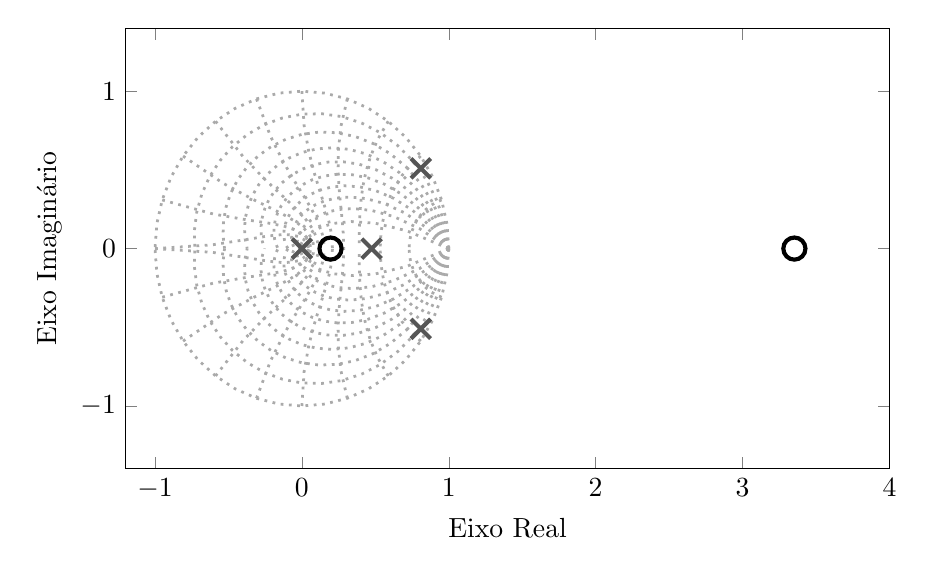
\begin{tikzpicture}

\begin{axis}[%
width=0.8\textwidth,
height=0.461611624834875\textwidth,
scale only axis,
xmin=-1.2,
xmax=4,
xtick={-1,  0,  1,  2,  3,  4},
xlabel={Eixo Real},
ymin=-1.4,
ymax=1.4,
ytick={-1,  0,  1},
ylabel={Eixo Imaginário}
]
\addplot [color=mycolor1,dotted,line width=1.0pt,forget plot]
  table[row sep=crcr]{1	0\\
0.987688340595138	0.156434465040231\\
0.951056516295154	0.309016994374947\\
0.891006524188368	0.453990499739547\\
0.809016994374947	0.587785252292473\\
0.707106781186548	0.707106781186547\\
0.587785252292473	0.809016994374947\\
0.453990499739547	0.891006524188368\\
0.309016994374947	0.951056516295154\\
0.156434465040231	0.987688340595138\\
6.12323399573677e-17	1\\
-0.156434465040231	0.987688340595138\\
-0.309016994374947	0.951056516295154\\
-0.453990499739547	0.891006524188368\\
-0.587785252292473	0.809016994374947\\
-0.707106781186547	0.707106781186548\\
-0.809016994374947	0.587785252292473\\
-0.891006524188368	0.453990499739547\\
-0.951056516295154	0.309016994374948\\
-0.987688340595138	0.156434465040231\\
-1	1.22464679914735e-16\\
};
\addplot [color=mycolor1,dotted,line width=1.0pt,forget plot]
  table[row sep=crcr]{1	0\\
0.972218045703082	0.153984211042097\\
0.921496791140463	0.299412457456957\\
0.849791018366557	0.432990150609548\\
0.759508516401756	0.551815237548133\\
0.653437051516106	0.653437051516106\\
0.534664304371591	0.735902282058355\\
0.406492952796512	0.797787339572243\\
0.272353130096494	0.83821674479613\\
0.135714483753824	0.856867527364047\\
5.22899666167123e-17	0.853959960588124\\
-0.131496350792703	0.830235283991667\\
-0.255686250369537	0.786921363444393\\
-0.369756251949576	0.725687504552447\\
-0.47122811850853	0.648589862732789\\
-0.558009078759514	0.558009078759514\\
-0.628431083783263	0.456581908289041\\
-0.681278445058817	0.347128705949459\\
-0.715803538350409	0.232578668243255\\
-0.731730559897045	0.115894735197653\\
-0.729247614287671	8.9307075662324e-17\\
};
\addplot [color=mycolor1,dotted,line width=1.0pt,forget plot]
  table[row sep=crcr]{1	0\\
0.956521682769877	0.151498151383791\\
0.891982039736211	0.289822533396298\\
0.809292583610082	0.412355167436434\\
0.711634858347723	0.517032989000692\\
0.602364630186427	0.602364630186426\\
0.484917701774751	0.667431957639199\\
0.362719588349683	0.711877274647591\\
0.239101059900595	0.735877395777214\\
0.117221283062812	0.740106053489981\\
4.44354699422903e-17	0.725686295399261\\
-0.109940132237539	0.694134676438339\\
-0.210320240583588	0.647299141978847\\
-0.299240493845688	0.587292536894097\\
-0.375203754387119	0.516423664031337\\
-0.437127756959533	0.437127756959533\\
-0.484346224770267	0.351898130574443\\
-0.516599582217932	0.263220634338226\\
-0.534016141209622	0.173512362385299\\
-0.537084820159711	0.0850658786478001\\
-0.526620599330303	6.44924231334916e-17\\
};
\addplot [color=mycolor1,dotted,line width=1.0pt,forget plot]
  table[row sep=crcr]{1	0\\
0.940082788364644	0.148894486293864\\
0.86158608093073	0.279946287694513\\
0.768279786681378	0.391458103646313\\
0.663960650859636	0.482395649771645\\
0.552351927561387	0.552351927561387\\
0.437014383712816	0.601498696728173\\
0.321269860940431	0.630527604183869\\
0.208138182971344	0.640583459188477\\
0.100287778328637	0.633192112325829\\
3.73630739569174e-17	0.610185303761559\\
-0.0908532273476425	0.573624701779294\\
-0.170819110593797	0.525727164509449\\
-0.238861981883349	0.468793035010043\\
-0.294350736089166	0.40513903143051\\
-0.337037028702328	0.337037028702328\\
-0.367025664975262	0.266659754473976\\
-0.384738677688982	0.196034147687371\\
-0.390874612629551	0.127002860400749\\
-0.386364521398959	0.0611941284830315\\
-0.372326104926586	4.55967972637346e-17\\
};
\addplot [color=mycolor1,dotted,line width=1.0pt,forget plot]
  table[row sep=crcr]{1	0\\
0.922246029428501	0.146069421212559\\
0.829201462983264	0.269423887468404\\
0.725373165529273	0.369596088217499\\
0.614985835074999	0.446813363302878\\
0.501902475185001	0.501902475185001\\
0.38956496084428	0.536190168955128\\
0.280953750703967	0.551402782692681\\
0.178565395716864	0.549567778706978\\
0.0844061798404073	0.532919645815306\\
3.08495992433718e-17	0.50381218919366\\
-0.0735915548753502	0.464638791061534\\
-0.135739038566523	0.417761804348184\\
-0.186207014322272	0.365451842507638\\
-0.225110018726605	0.309837359892227\\
-0.252864584784672	0.252864584784672\\
-0.270139142845401	0.196267575756099\\
-0.277803443075876	0.141547924204336\\
-0.27687894570066	0.0899634229303457\\
-0.268491413422519	0.0425248622468694\\
-0.253826721980109	3.10848082611005e-17\\
};
\addplot [color=mycolor1,dotted,line width=1.0pt,forget plot]
  table[row sep=crcr]{1	0\\
0.902056570675584	0.142871725087523\\
0.793293726869509	0.257756756757911\\
0.678769666307395	0.345850419328459\\
0.562876391436159	0.408953636388562\\
0.449318435861499	0.449318435861499\\
0.341115747349381	0.469505547439701\\
0.24062663375655	0.472256359314945\\
0.149586755320764	0.460380694230177\\
0.069160331541479	0.436661148025441\\
2.47240337905553e-17	0.403774113610049\\
-0.057687904157153	0.364227092250654\\
-0.104075505986926	0.320311471399148\\
-0.139645446506012	0.274069620358657\\
-0.165124892040398	0.227274916024158\\
-0.18142315316863	0.18142315316863\\
-0.189574186252466	0.137733708524426\\
-0.190684892879101	0.0971588057560207\\
-0.185889806735969	0.0603992595374446\\
-0.176312467991919	0.0279251515651378\\
-0.16303353482158	1.99658496572927e-17\\
};
\addplot [color=mycolor1,dotted,line width=1.0pt,forget plot]
  table[row sep=crcr]{1	0\\
0.877921760602431	0.139049146701748\\
0.751411952540787	0.244148543365328\\
0.625732257688895	0.318826509862098\\
0.505011411193747	0.36691226736026\\
0.392341669548685	0.392341669548685\\
0.289890514921595	0.399000063654162\\
0.199020572856858	0.390599867100522\\
0.120411913496453	0.370589763847805\\
0.0541820486548744	0.34209199176291\\
1.88512313530119e-17	0.307863971328499\\
-0.042808222513439	0.270280479734772\\
-0.075164540154518	0.231332667812908\\
-0.0981551954909503	0.192640417840451\\
-0.112959067758674	0.155474818616317\\
-0.120787864504912	0.120787864504912\\
-0.122837744156894	0.0892468451742257\\
-0.120251626285951	0.0612712639357851\\
-0.114091236431876	0.0370704898842818\\
-0.105317799143806	0.0166807006736036\\
-0.0947802248421549	1.16072298975411e-17\\
};
\addplot [color=mycolor1,dotted,line width=1.0pt,forget plot]
  table[row sep=crcr]{1	0\\
0.84674396664984	0.134111069256013\\
0.698989566160914	0.227115477506975\\
0.561406498364893	0.286050898428465\\
0.437004973478602	0.317502698182059\\
0.327450698344114	0.327450698344114\\
0.233352139914598	0.321181666481713\\
0.154515499860225	0.303253743289057\\
0.0901653834921457	0.27750051639687\\
0.0391311034995635	0.247064063991275\\
1.31311479217367e-17	0.214447919692096\\
-0.0287598398096346	0.181582482159892\\
-0.0487044416812479	0.149896858349689\\
-0.0613430200940395	0.120392455675976\\
-0.06808779312177	0.0937148074575858\\
-0.0702211210616195	0.0702211210616195\\
-0.068876740220244	0.0500418809603846\\
-0.0650321343871793	0.0331355275052096\\
-0.0595094084547913	0.0193357789181307\\
-0.0529823745536039	0.00839158374073751\\
-0.0459879102602678	5.63189470997126e-18\\
};
\addplot [color=mycolor1,dotted,line width=1.0pt,forget plot]
  table[row sep=crcr]{1	0\\
0.801053465278425	0.126874404768154\\
0.625589539649299	0.203266363189334\\
0.475341369738971	0.242198525079547\\
0.350045057714404	0.254322621147605\\
0.24813777530853	0.24813777530853\\
0.167289292234614	0.230253957320141\\
0.104794333468008	0.205670459781722\\
0.0578515468028918	0.178048753195384\\
0.0237523524567972	0.149966451301199\\
7.54043881219821e-18	0.123144711070133\\
-0.0156239119173694	0.0986454975334405\\
-0.0250311775652273	0.0770380431086105\\
-0.0298254673925332	0.0585357756361869\\
-0.0313184856998208	0.0431061974937683\\
-0.0305568546459545	0.0305568546459545\\
-0.0283545570469435	0.0206007915573586\\
-0.0253272293454815	0.012904867916705\\
-0.021925762268643	0.00712411201600239\\
-0.0184675753156993	0.00292497658052826\\
-0.0151646198645466	1.85713031774033e-18\\
};
\addplot [color=mycolor1,dotted,line width=1.0pt,forget plot]
  table[row sep=crcr]{1	0\\
0.714110955679367	0.113104064044896\\
0.497161927717827	0.161537702532642\\
0.336758208677056	0.171586877647116\\
0.221075553032581	0.160620791180475\\
0.139705610200823	0.139705610200823\\
0.0839640345306934	0.115566579097864\\
0.0468885871776745	0.0920240337831981\\
0.0230753615892199	0.0710186604775083\\
0.00844586939409394	0.0533251206797082\\
2.39022368106624e-18	0.0390353150431684\\
-0.00441505277265522	0.0278755461307222\\
-0.00630567510971132	0.0194068724759343\\
-0.00669794782622876	0.0131454627690819\\
-0.0062698831862128	0.00862975386096949\\
-0.0054534525074872	0.0054534525074872\\
-0.00451117782354635	0.00327756254020109\\
-0.00359218715027031	0.00183031077240959\\
-0.00277223578568335	0.000900754009370227\\
-0.00208156288544739	0.000329687172611911\\
-0.00152375582051941	1.86606268828125e-19\\
};
\addplot [color=mycolor1,dotted,line width=1.0pt,forget plot]
  table[row sep=crcr]{1	-0\\
0.987688340595138	-0.156434465040231\\
0.951056516295154	-0.309016994374947\\
0.891006524188368	-0.453990499739547\\
0.809016994374947	-0.587785252292473\\
0.707106781186548	-0.707106781186547\\
0.587785252292473	-0.809016994374947\\
0.453990499739547	-0.891006524188368\\
0.309016994374947	-0.951056516295154\\
0.156434465040231	-0.987688340595138\\
6.12323399573677e-17	-1\\
-0.156434465040231	-0.987688340595138\\
-0.309016994374947	-0.951056516295154\\
-0.453990499739547	-0.891006524188368\\
-0.587785252292473	-0.809016994374947\\
-0.707106781186547	-0.707106781186548\\
-0.809016994374947	-0.587785252292473\\
-0.891006524188368	-0.453990499739547\\
-0.951056516295154	-0.309016994374948\\
-0.987688340595138	-0.156434465040231\\
-1	-1.22464679914735e-16\\
};
\addplot [color=mycolor1,dotted,line width=1.0pt,forget plot]
  table[row sep=crcr]{1	-0\\
0.972218045703082	-0.153984211042097\\
0.921496791140463	-0.299412457456957\\
0.849791018366557	-0.432990150609548\\
0.759508516401756	-0.551815237548133\\
0.653437051516106	-0.653437051516106\\
0.534664304371591	-0.735902282058355\\
0.406492952796512	-0.797787339572243\\
0.272353130096494	-0.83821674479613\\
0.135714483753824	-0.856867527364047\\
5.22899666167123e-17	-0.853959960588124\\
-0.131496350792703	-0.830235283991667\\
-0.255686250369537	-0.786921363444393\\
-0.369756251949576	-0.725687504552447\\
-0.47122811850853	-0.648589862732789\\
-0.558009078759514	-0.558009078759514\\
-0.628431083783263	-0.456581908289041\\
-0.681278445058817	-0.347128705949459\\
-0.715803538350409	-0.232578668243255\\
-0.731730559897045	-0.115894735197653\\
-0.729247614287671	-8.9307075662324e-17\\
};
\addplot [color=mycolor1,dotted,line width=1.0pt,forget plot]
  table[row sep=crcr]{1	-0\\
0.956521682769877	-0.151498151383791\\
0.891982039736211	-0.289822533396298\\
0.809292583610082	-0.412355167436434\\
0.711634858347723	-0.517032989000692\\
0.602364630186427	-0.602364630186426\\
0.484917701774751	-0.667431957639199\\
0.362719588349683	-0.711877274647591\\
0.239101059900595	-0.735877395777214\\
0.117221283062812	-0.740106053489981\\
4.44354699422903e-17	-0.725686295399261\\
-0.109940132237539	-0.694134676438339\\
-0.210320240583588	-0.647299141978847\\
-0.299240493845688	-0.587292536894097\\
-0.375203754387119	-0.516423664031337\\
-0.437127756959533	-0.437127756959533\\
-0.484346224770267	-0.351898130574443\\
-0.516599582217932	-0.263220634338226\\
-0.534016141209622	-0.173512362385299\\
-0.537084820159711	-0.0850658786478001\\
-0.526620599330303	-6.44924231334916e-17\\
};
\addplot [color=mycolor1,dotted,line width=1.0pt,forget plot]
  table[row sep=crcr]{1	-0\\
0.940082788364644	-0.148894486293864\\
0.86158608093073	-0.279946287694513\\
0.768279786681378	-0.391458103646313\\
0.663960650859636	-0.482395649771645\\
0.552351927561387	-0.552351927561387\\
0.437014383712816	-0.601498696728173\\
0.321269860940431	-0.630527604183869\\
0.208138182971344	-0.640583459188477\\
0.100287778328637	-0.633192112325829\\
3.73630739569174e-17	-0.610185303761559\\
-0.0908532273476425	-0.573624701779294\\
-0.170819110593797	-0.525727164509449\\
-0.238861981883349	-0.468793035010043\\
-0.294350736089166	-0.40513903143051\\
-0.337037028702328	-0.337037028702328\\
-0.367025664975262	-0.266659754473976\\
-0.384738677688982	-0.196034147687371\\
-0.390874612629551	-0.127002860400749\\
-0.386364521398959	-0.0611941284830315\\
-0.372326104926586	-4.55967972637346e-17\\
};
\addplot [color=mycolor1,dotted,line width=1.0pt,forget plot]
  table[row sep=crcr]{1	-0\\
0.922246029428501	-0.146069421212559\\
0.829201462983264	-0.269423887468404\\
0.725373165529273	-0.369596088217499\\
0.614985835074999	-0.446813363302878\\
0.501902475185001	-0.501902475185001\\
0.38956496084428	-0.536190168955128\\
0.280953750703967	-0.551402782692681\\
0.178565395716864	-0.549567778706978\\
0.0844061798404073	-0.532919645815306\\
3.08495992433718e-17	-0.50381218919366\\
-0.0735915548753502	-0.464638791061534\\
-0.135739038566523	-0.417761804348184\\
-0.186207014322272	-0.365451842507638\\
-0.225110018726605	-0.309837359892227\\
-0.252864584784672	-0.252864584784672\\
-0.270139142845401	-0.196267575756099\\
-0.277803443075876	-0.141547924204336\\
-0.27687894570066	-0.0899634229303457\\
-0.268491413422519	-0.0425248622468694\\
-0.253826721980109	-3.10848082611005e-17\\
};
\addplot [color=mycolor1,dotted,line width=1.0pt,forget plot]
  table[row sep=crcr]{1	-0\\
0.902056570675584	-0.142871725087523\\
0.793293726869509	-0.257756756757911\\
0.678769666307395	-0.345850419328459\\
0.562876391436159	-0.408953636388562\\
0.449318435861499	-0.449318435861499\\
0.341115747349381	-0.469505547439701\\
0.24062663375655	-0.472256359314945\\
0.149586755320764	-0.460380694230177\\
0.069160331541479	-0.436661148025441\\
2.47240337905553e-17	-0.403774113610049\\
-0.057687904157153	-0.364227092250654\\
-0.104075505986926	-0.320311471399148\\
-0.139645446506012	-0.274069620358657\\
-0.165124892040398	-0.227274916024158\\
-0.18142315316863	-0.18142315316863\\
-0.189574186252466	-0.137733708524426\\
-0.190684892879101	-0.0971588057560207\\
-0.185889806735969	-0.0603992595374446\\
-0.176312467991919	-0.0279251515651378\\
-0.16303353482158	-1.99658496572927e-17\\
};
\addplot [color=mycolor1,dotted,line width=1.0pt,forget plot]
  table[row sep=crcr]{1	-0\\
0.877921760602431	-0.139049146701748\\
0.751411952540787	-0.244148543365328\\
0.625732257688895	-0.318826509862098\\
0.505011411193747	-0.36691226736026\\
0.392341669548685	-0.392341669548685\\
0.289890514921595	-0.399000063654162\\
0.199020572856858	-0.390599867100522\\
0.120411913496453	-0.370589763847805\\
0.0541820486548744	-0.34209199176291\\
1.88512313530119e-17	-0.307863971328499\\
-0.042808222513439	-0.270280479734772\\
-0.075164540154518	-0.231332667812908\\
-0.0981551954909503	-0.192640417840451\\
-0.112959067758674	-0.155474818616317\\
-0.120787864504912	-0.120787864504912\\
-0.122837744156894	-0.0892468451742257\\
-0.120251626285951	-0.0612712639357851\\
-0.114091236431876	-0.0370704898842818\\
-0.105317799143806	-0.0166807006736036\\
-0.0947802248421549	-1.16072298975411e-17\\
};
\addplot [color=mycolor1,dotted,line width=1.0pt,forget plot]
  table[row sep=crcr]{1	-0\\
0.84674396664984	-0.134111069256013\\
0.698989566160914	-0.227115477506975\\
0.561406498364893	-0.286050898428465\\
0.437004973478602	-0.317502698182059\\
0.327450698344114	-0.327450698344114\\
0.233352139914598	-0.321181666481713\\
0.154515499860225	-0.303253743289057\\
0.0901653834921457	-0.27750051639687\\
0.0391311034995635	-0.247064063991275\\
1.31311479217367e-17	-0.214447919692096\\
-0.0287598398096346	-0.181582482159892\\
-0.0487044416812479	-0.149896858349689\\
-0.0613430200940395	-0.120392455675976\\
-0.06808779312177	-0.0937148074575858\\
-0.0702211210616195	-0.0702211210616195\\
-0.068876740220244	-0.0500418809603846\\
-0.0650321343871793	-0.0331355275052096\\
-0.0595094084547913	-0.0193357789181307\\
-0.0529823745536039	-0.00839158374073751\\
-0.0459879102602678	-5.63189470997126e-18\\
};
\addplot [color=mycolor1,dotted,line width=1.0pt,forget plot]
  table[row sep=crcr]{1	-0\\
0.801053465278425	-0.126874404768154\\
0.625589539649299	-0.203266363189334\\
0.475341369738971	-0.242198525079547\\
0.350045057714404	-0.254322621147605\\
0.24813777530853	-0.24813777530853\\
0.167289292234614	-0.230253957320141\\
0.104794333468008	-0.205670459781722\\
0.0578515468028918	-0.178048753195384\\
0.0237523524567972	-0.149966451301199\\
7.54043881219821e-18	-0.123144711070133\\
-0.0156239119173694	-0.0986454975334405\\
-0.0250311775652273	-0.0770380431086105\\
-0.0298254673925332	-0.0585357756361869\\
-0.0313184856998208	-0.0431061974937683\\
-0.0305568546459545	-0.0305568546459545\\
-0.0283545570469435	-0.0206007915573586\\
-0.0253272293454815	-0.012904867916705\\
-0.021925762268643	-0.00712411201600239\\
-0.0184675753156993	-0.00292497658052826\\
-0.0151646198645466	-1.85713031774033e-18\\
};
\addplot [color=mycolor1,dotted,line width=1.0pt,forget plot]
  table[row sep=crcr]{1	-0\\
0.714110955679367	-0.113104064044896\\
0.497161927717827	-0.161537702532642\\
0.336758208677056	-0.171586877647116\\
0.221075553032581	-0.160620791180475\\
0.139705610200823	-0.139705610200823\\
0.0839640345306934	-0.115566579097864\\
0.0468885871776745	-0.0920240337831981\\
0.0230753615892199	-0.0710186604775083\\
0.00844586939409394	-0.0533251206797082\\
2.39022368106624e-18	-0.0390353150431684\\
-0.00441505277265522	-0.0278755461307222\\
-0.00630567510971132	-0.0194068724759343\\
-0.00669794782622876	-0.0131454627690819\\
-0.0062698831862128	-0.00862975386096949\\
-0.0054534525074872	-0.0054534525074872\\
-0.00451117782354635	-0.00327756254020109\\
-0.00359218715027031	-0.00183031077240959\\
-0.00277223578568335	-0.000900754009370227\\
-0.00208156288544739	-0.000329687172611911\\
-0.00152375582051941	-1.86606268828125e-19\\
};
\addplot [color=mycolor1,dotted,line width=1.0pt,forget plot]
  table[row sep=crcr]{1	0\\
1	0\\
};
\addplot [color=mycolor1,dotted,line width=1.0pt,forget plot]
  table[row sep=crcr]{0.951056516295154	0.309016994374947\\
0.906577591518048	0.290693092532446\\
0.867277205719189	0.267124444629623\\
0.833330533437629	0.239553777474139\\
0.804679893747523	0.20903820245934\\
0.781122098933164	0.176433510213537\\
0.762382187756933	0.142402376999381\\
0.748171074803624	0.107437628337747\\
0.738227708485823	0.0718935522249012\\
0.732347931289196	0.0360204899377399\\
0.730402691048646	2.81010850277162e-17\\
};
\addplot [color=mycolor1,dotted,line width=1.0pt,forget plot]
  table[row sep=crcr]{0.809016994374947	0.587785252292473\\
0.737380455396588	0.527071687397996\\
0.6808142826414	0.463341883835339\\
0.637053765657314	0.399254954339046\\
0.603812761314093	0.336417677088311\\
0.579022949915482	0.275632227640288\\
0.560948163233974	0.217130071437151\\
0.54821711318997	0.160763451735608\\
0.539811466724715	0.106147624627789\\
0.535036016768209	0.0527590625798542\\
0.533488091091103	4.10502162512614e-17\\
};
\addplot [color=mycolor1,dotted,line width=1.0pt,forget plot]
  table[row sep=crcr]{0.587785252292473	0.809016994374947\\
0.515276498489902	0.692182785870847\\
0.46668476526979	0.583707991451876\\
0.435233321876477	0.485319980094308\\
0.415551842123536	0.396928474901319\\
0.403656860517901	0.317461475735791\\
0.396737049613855	0.245416450708029\\
0.392888142823216	0.179177710929467\\
0.39087245229983	0.11717008156476\\
0.389932112762627	0.0579102497954412\\
0.389661137375347	4.49747826270753e-17\\
};
\addplot [color=mycolor1,dotted,line width=1.0pt,forget plot]
  table[row sep=crcr]{0.309016994374947	0.951056516295154\\
0.265925372344309	0.777304721760365\\
0.248822386132444	0.630899544522142\\
0.24643298177389	0.508693744238057\\
0.251412997268255	0.406266573115132\\
0.25929445161488	0.31919477108011\\
0.267517373913267	0.243597429511063\\
0.274697115780397	0.1762665508339\\
0.280129101393366	0.114599409879343\\
0.283480020554887	0.0564559973822998\\
0.284609543336029	4.37996030135249e-17\\
};
\addplot [color=mycolor1,dotted,line width=1.0pt,forget plot]
  table[row sep=crcr]{6.12323399573677e-17	1\\
0.0151248701748503	0.781989711398728\\
0.0472692933177679	0.613631335769719\\
0.0835006201485716	0.482943980920436\\
0.117381749765263	0.379469463911326\\
0.146223972383669	0.295078319831894\\
0.169261627793672	0.223809451176491\\
0.186582776182006	0.161390341419992\\
0.198560105942714	0.104739935929793\\
0.205572433929556	0.0515565221197431\\
0.207879576350762	3.99891848849262e-17\\
};
\addplot [color=mycolor1,dotted,line width=1.0pt,forget plot]
  table[row sep=crcr]{-0.309016994374947	0.951056516295154\\
-0.213607139159912	0.713331044437031\\
-0.122920349149865	0.544815253953639\\
-0.0461074386071066	0.422454854218942\\
0.0151311193047769	0.329888717873058\\
0.0621570724668225	0.256291005261778\\
0.0971710522581798	0.194731597161215\\
0.122256440677152	0.140793596164787\\
0.13905244595299	0.0915971142347777\\
0.148693455532156	0.0451621321066958\\
0.151835801980649	3.50498499033503e-17\\
};
\addplot [color=mycolor1,dotted,line width=1.0pt,forget plot]
  table[row sep=crcr]{-0.587785252292473	0.809016994374948\\
-0.401011853057454	0.584595820351374\\
-0.252139489074835	0.439670821081765\\
-0.139623392550337	0.340999317931598\\
-0.0567836371213516	0.268617800427267\\
0.0033339412143336	0.21116115844769\\
0.0463512370945915	0.162297289886265\\
0.0763422025660035	0.118472638203443\\
0.0960671266193367	0.0776165020305757\\
0.1072685824301	0.0384304051397518\\
0.110901278364195	2.98672554719679e-17\\
};
\addplot [color=mycolor1,dotted,line width=1.0pt,forget plot]
  table[row sep=crcr]{-0.809016994374948	0.587785252292473\\
-0.533486326814499	0.413410095118228\\
-0.336121655437603	0.313963860155743\\
-0.198040110920963	0.250717832404618\\
-0.101844033235305	0.204281393673556\\
-0.0346516892466227	0.165530866251108\\
0.0122258376810533	0.130333089269644\\
0.0443886084751889	0.0968398262452624\\
0.065339288702761	0.0642052594194206\\
0.0771736424133687	0.032008294596762\\
0.0810025921579431	2.49315700239574e-17\\
};
\addplot [color=mycolor1,dotted,line width=1.0pt,forget plot]
  table[row sep=crcr]{-0.951056516295154	0.309016994374948\\
-0.60382220830535	0.219707538176049\\
-0.375378071887508	0.182507388795924\\
-0.225093275108467	0.161489568357552\\
-0.124654461172013	0.143091836517116\\
-0.0562723920172722	0.12318609851568\\
-0.00923898083522721	0.101104614081101\\
0.0228060316514889	0.0772217637055013\\
0.0436193292019494	0.0520955750986265\\
0.0553650029180358	0.0262210407420432\\
0.0591645112940776	2.0486346567262e-17\\
};
\addplot [color=mycolor1,dotted,line width=1.0pt,forget plot]
  table[row sep=crcr]{-1	1.22464679914735e-16\\
-0.61127914703566	0.0236549857259488\\
-0.374309030147768	0.0580118391989452\\
-0.226262535142082	0.0806522438077526\\
-0.130218598863194	0.0890855793127953\\
-0.0656897647351535	0.0862950481802363\\
-0.0214411717925588	0.0757647040434823\\
0.00876629006412298	0.0602253159022079\\
0.0284556614934045	0.0415943455493057\\
0.039601950618638	0.0211971994741971\\
0.0432139182637723	1.66258696249815e-17\\
};
\addplot [color=mycolor1,dotted,line width=1.0pt,forget plot]
  table[row sep=crcr]{1	-0\\
1	-0\\
};
\addplot [color=mycolor1,dotted,line width=1.0pt,forget plot]
  table[row sep=crcr]{0.951056516295154	-0.309016994374947\\
0.906577591518048	-0.290693092532446\\
0.867277205719189	-0.267124444629623\\
0.833330533437629	-0.239553777474139\\
0.804679893747523	-0.20903820245934\\
0.781122098933164	-0.176433510213537\\
0.762382187756933	-0.142402376999381\\
0.748171074803624	-0.107437628337747\\
0.738227708485823	-0.0718935522249012\\
0.732347931289196	-0.0360204899377399\\
0.730402691048646	-2.81010850277162e-17\\
};
\addplot [color=mycolor1,dotted,line width=1.0pt,forget plot]
  table[row sep=crcr]{0.809016994374947	-0.587785252292473\\
0.737380455396588	-0.527071687397996\\
0.6808142826414	-0.463341883835339\\
0.637053765657314	-0.399254954339046\\
0.603812761314093	-0.336417677088311\\
0.579022949915482	-0.275632227640288\\
0.560948163233974	-0.217130071437151\\
0.54821711318997	-0.160763451735608\\
0.539811466724715	-0.106147624627789\\
0.535036016768209	-0.0527590625798542\\
0.533488091091103	-4.10502162512614e-17\\
};
\addplot [color=mycolor1,dotted,line width=1.0pt,forget plot]
  table[row sep=crcr]{0.587785252292473	-0.809016994374947\\
0.515276498489902	-0.692182785870847\\
0.46668476526979	-0.583707991451876\\
0.435233321876477	-0.485319980094308\\
0.415551842123536	-0.396928474901319\\
0.403656860517901	-0.317461475735791\\
0.396737049613855	-0.245416450708029\\
0.392888142823216	-0.179177710929467\\
0.39087245229983	-0.11717008156476\\
0.389932112762627	-0.0579102497954412\\
0.389661137375347	-4.49747826270753e-17\\
};
\addplot [color=mycolor1,dotted,line width=1.0pt,forget plot]
  table[row sep=crcr]{0.309016994374947	-0.951056516295154\\
0.265925372344309	-0.777304721760365\\
0.248822386132444	-0.630899544522142\\
0.24643298177389	-0.508693744238057\\
0.251412997268255	-0.406266573115132\\
0.25929445161488	-0.31919477108011\\
0.267517373913267	-0.243597429511063\\
0.274697115780397	-0.1762665508339\\
0.280129101393366	-0.114599409879343\\
0.283480020554887	-0.0564559973822998\\
0.284609543336029	-4.37996030135249e-17\\
};
\addplot [color=mycolor1,dotted,line width=1.0pt,forget plot]
  table[row sep=crcr]{6.12323399573677e-17	-1\\
0.0151248701748503	-0.781989711398728\\
0.0472692933177679	-0.613631335769719\\
0.0835006201485716	-0.482943980920436\\
0.117381749765263	-0.379469463911326\\
0.146223972383669	-0.295078319831894\\
0.169261627793672	-0.223809451176491\\
0.186582776182006	-0.161390341419992\\
0.198560105942714	-0.104739935929793\\
0.205572433929556	-0.0515565221197431\\
0.207879576350762	-3.99891848849262e-17\\
};
\addplot [color=mycolor1,dotted,line width=1.0pt,forget plot]
  table[row sep=crcr]{-0.309016994374947	-0.951056516295154\\
-0.213607139159912	-0.713331044437031\\
-0.122920349149865	-0.544815253953639\\
-0.0461074386071066	-0.422454854218942\\
0.0151311193047769	-0.329888717873058\\
0.0621570724668225	-0.256291005261778\\
0.0971710522581798	-0.194731597161215\\
0.122256440677152	-0.140793596164787\\
0.13905244595299	-0.0915971142347777\\
0.148693455532156	-0.0451621321066958\\
0.151835801980649	-3.50498499033503e-17\\
};
\addplot [color=mycolor1,dotted,line width=1.0pt,forget plot]
  table[row sep=crcr]{-0.587785252292473	-0.809016994374948\\
-0.401011853057454	-0.584595820351374\\
-0.252139489074835	-0.439670821081765\\
-0.139623392550337	-0.340999317931598\\
-0.0567836371213516	-0.268617800427267\\
0.0033339412143336	-0.21116115844769\\
0.0463512370945915	-0.162297289886265\\
0.0763422025660035	-0.118472638203443\\
0.0960671266193367	-0.0776165020305757\\
0.1072685824301	-0.0384304051397518\\
0.110901278364195	-2.98672554719679e-17\\
};
\addplot [color=mycolor1,dotted,line width=1.0pt,forget plot]
  table[row sep=crcr]{-0.809016994374948	-0.587785252292473\\
-0.533486326814499	-0.413410095118228\\
-0.336121655437603	-0.313963860155743\\
-0.198040110920963	-0.250717832404618\\
-0.101844033235305	-0.204281393673556\\
-0.0346516892466227	-0.165530866251108\\
0.0122258376810533	-0.130333089269644\\
0.0443886084751889	-0.0968398262452624\\
0.065339288702761	-0.0642052594194206\\
0.0771736424133687	-0.032008294596762\\
0.0810025921579431	-2.49315700239574e-17\\
};
\addplot [color=mycolor1,dotted,line width=1.0pt,forget plot]
  table[row sep=crcr]{-0.951056516295154	-0.309016994374948\\
-0.60382220830535	-0.219707538176049\\
-0.375378071887508	-0.182507388795924\\
-0.225093275108467	-0.161489568357552\\
-0.124654461172013	-0.143091836517116\\
-0.0562723920172722	-0.12318609851568\\
-0.00923898083522721	-0.101104614081101\\
0.0228060316514889	-0.0772217637055013\\
0.0436193292019494	-0.0520955750986265\\
0.0553650029180358	-0.0262210407420432\\
0.0591645112940776	-2.0486346567262e-17\\
};
\addplot [color=mycolor1,dotted,line width=1.0pt,forget plot]
  table[row sep=crcr]{-1	-1.22464679914735e-16\\
-0.61127914703566	-0.0236549857259488\\
-0.374309030147768	-0.0580118391989452\\
-0.226262535142082	-0.0806522438077526\\
-0.130218598863194	-0.0890855793127953\\
-0.0656897647351535	-0.0862950481802363\\
-0.0214411717925588	-0.0757647040434823\\
0.00876629006412298	-0.0602253159022079\\
0.0284556614934045	-0.0415943455493057\\
0.039601950618638	-0.0211971994741971\\
0.0432139182637723	-1.66258696249815e-17\\
};
\addplot [color=black!50!mycolor1,line width=1.5pt,mark size=5.0pt,only marks,mark=x,mark options={solid},forget plot]
  table[row sep=crcr]{0	0\\
0.809915206392298	0.509761287368869\\
0.809915206392298	-0.509761287368869\\
0.474723347707754	0\\
};
\addplot [color=black,line width=1.5pt,mark size=4.0pt,only marks,mark=o,mark options={solid},forget plot]
  table[row sep=crcr]{3.35287627897953	0\\
0.194909709644537	0\\
};
\end{axis}
\end{tikzpicture}%}
    \captionof{figure}{Diagrama de pólos e zeros para $\Delta(z)$ para $v_C$ como variável intermediária.}
    \label{fig:pzmap_delta_vc}
  \end{minipage}
  \vspace{1cm}

  % \begin{figure}[htb]
  %   \centering
  %   \subfloat[Margem de ganho para $G(z)$, $G_o(z)$ e $\Delta(z)$.]{\label{fig:mag_g_go_delta_vc}
  %     {\def\svgwidth{0.8\textwidth}% This file was created by matlab2tikz v0.4.7 running on MATLAB 8.3.
% Copyright (c) 2008--2014, Nico Schlömer <nico.schloemer@gmail.com>
% All rights reserved.
% Minimal pgfplots version: 1.3
% 
% The latest updates can be retrieved from
%   http://www.mathworks.com/matlabcentral/fileexchange/22022-matlab2tikz
% where you can also make suggestions and rate matlab2tikz.
% 
%
% defining custom colors
\definecolor{mycolor1}{rgb}{0.33333,0.33333,0.33333}%
%
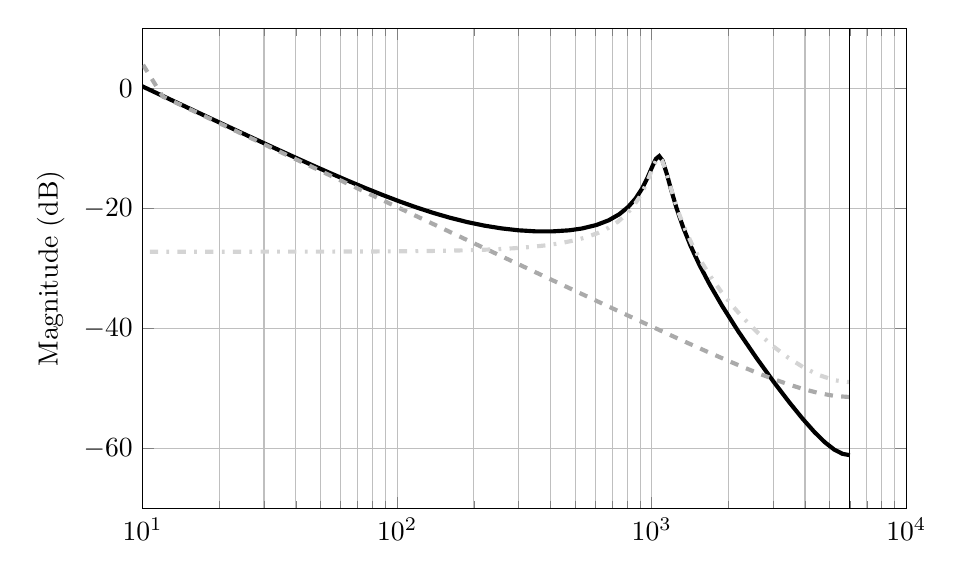
\begin{tikzpicture}

\begin{axis}[%
width=0.8\textwidth,
height=0.503129594988472\textwidth,
scale only axis,
xmode=log,
xmin=10,
xmax=10000,
xminorticks=true,
xmajorgrids,
xminorgrids,
ymin=-70,
ymax=10,
ylabel={Magnitude (dB)},
ymajorgrids
]
\addplot [color=black,solid,line width=1.5pt,forget plot]
  table[row sep=crcr]{8.72405426743874	1.48363673726623\\
10.1733925633752	0.151765865562977\\
11.8635112845217	-1.17900050571652\\
13.8344115909431	-2.50826758358683\\
16.1327400865988	-3.83550075892022\\
18.812892835438	-5.15997718177271\\
21.938302789101	-6.48072147799965\\
25.5829410966331	-7.79642117597815\\
29.8330678286992	-9.1053168201851\\
34.7892735518555	-10.4050616792364\\
40.5688600721623	-11.6925470642498\\
47.3086166947834	-12.963692640246\\
55.1680577071395	-14.2132083269884\\
64.3331977092853	-15.4343473773203\\
75.0209541447453	-16.6186904629486\\
87.4842812294358	-17.7560270853601\\
102.01815678676	-18.8344262881613\\
118.966563683284	-19.8405962564975\\
138.730631099244	-20.7605945123435\\
161.778128318745	-21.5808412495891\\
188.654535735468	-22.2892112666733\\
219.995955098717	-22.8757939443754\\
256.544164555156	-23.3328141668633\\
299.1641748039	-23.6532532955861\\
348.864701878087	-23.8278040901056\\
406.822041095882	-23.8396636362778\\
474.40790722145	-23.6558609728876\\
531.504182204689	-23.3579539039264\\
606.064869421581	-22.775432926242\\
677.501516549994	-21.9884444085573\\
744.70428505611	-20.9962386513889\\
806.949577729217	-19.7928078790731\\
863.84758836883	-18.3718357326149\\
915.278419070289	-16.7380060428108\\
961.327424257804	-14.9386697886322\\
1002.22625276946	-13.1427152242176\\
1038.30279972218	-11.7561240986035\\
1069.94103119274	-11.3051731976108\\
1102.54331447059	-12.0391127184131\\
1142.23091549082	-14.0621076501556\\
1190.82612369414	-16.868091817206\\
1250.73833969845	-19.9328845545705\\
1325.20345677115	-23.0451462598858\\
1418.64354579777	-26.1773289433106\\
1537.21931403086	-29.3712811406372\\
1689.69925862198	-32.6940870263255\\
1888.86349958272	-36.2248746323424\\
2153.83782208684	-40.0506176653624\\
2206.10594744096	-40.7212633302711\\
2572.60915071119	-44.8654596914697\\
3000	-48.7881593135897\\
3030.2689591777	-49.037265378468\\
3469.23953517283	-52.3021760581578\\
3912.38254234155	-55.0286589568067\\
4353.43031613188	-57.2474602051834\\
4786.88753737426	-58.9653377079392\\
5208.13303270343	-60.177300914054\\
5613.4498161518	-60.8837343303444\\
6000	-61.1085317362432\\
};
\addplot [color=black,solid,forget plot]
  table[row sep=crcr]{6000	-78\\
6000	-60\\
6000	0\\
6000	18\\
};
\addplot [color=mycolor1,dashed,line width=1.5pt,forget plot]
  table[row sep=crcr]{6.24758082087633	18\\
12	-1.36840782695356\\
120	-21.3669932960897\\
132.294888466487	-22.213921867537\\
145.849479286335	-23.0607841297459\\
160.79283829234	-23.9075657960853\\
177.267255067459	-24.754249501069\\
195.429597815914	-25.6008141364939\\
215.45280705089	-26.4472340442679\\
237.527542321575	-27.2934780349128\\
261.863997659596	-28.1395081939741\\
288.693903031372	-28.9852784303313\\
318.272730854084	-29.8307327103401\\
350.882128585544	-30.6758029094342\\
386.8326005509	-31.5204061977516\\
426.466464542353	-32.364441857884\\
470.161111344397	-33.2077874101628\\
518.332598221554	-34.0502938929742\\
571.43961058554	-34.8917801111303\\
629.987829564556	-35.7320256226589\\
694.534747062392	-36.5707621813492\\
765.69497415599	-37.4076632862154\\
844.146093377636	-38.2423314060069\\
930.63511060679	-39.0742823420868\\
1025.98556800602	-39.9029260597625\\
1131.10538572984	-40.7275431473702\\
1246.99550707477	-41.5472558414477\\
1374.75942938889	-42.3609922673178\\
1515.61371149379	-43.1674421617671\\
1670.89955766957	-43.9650018309287\\
1842.09558850499	-44.7517053965228\\
2030.83192021562	-45.5251384133725\\
2238.90568649256	-46.2823285708213\\
2468.2981506793	-47.0196062151881\\
2721.19357121795	-47.7324245172266\\
3000	-48.4151247041515\\
3446.0950649911	-49.3193163438247\\
3958.52373231868	-50.1208986469465\\
4547.14969953119	-50.7813694824215\\
5223.30337977675	-51.2446073163611\\
6000	-51.4254246607914\\
};
\addplot [color=black,solid,forget plot]
  table[row sep=crcr]{6000	-78\\
6000	-60\\
6000	0\\
6000	18\\
};
\addplot [color=white!50!mycolor1,dash pattern=on 1pt off 3pt on 3pt off 3pt,line width=1.5pt,forget plot]
  table[row sep=crcr]{2.15231873701794	-27.2200078055767\\
21.5231873701794	-27.2169614554126\\
24.6869879475792	-27.2159900128982\\
28.3158513393938	-27.2147117566695\\
32.4781394464639	-27.2130296897135\\
37.2522630261321	-27.2108160805587\\
42.7281588237413	-27.2079026739111\\
49.0089838350534	-27.2040677460686\\
56.2130586167442	-27.1990189610352\\
64.4760962537936	-27.1923706181034\\
73.9537589739008	-27.1836133747875\\
84.8245905713938	-27.1720738156951\\
97.2933798827434	-27.1568602178018\\
111.595018676107	-27.1367893759959\\
127.998926631282	-27.1102871395801\\
146.814126769514	-27.0752519361927\\
168.395066946031	-27.0288652793856\\
193.148297072777	-26.9673247563754\\
221.540127859386	-26.8854608846303\\
254.105415350673	-26.7761750099871\\
291.45763674706	-26.6295922582879\\
334.300447320066	-26.4317432131382\\
383.440936136402	-26.1624305395138\\
439.804830307013	-25.7916082494815\\
504.453934184461	-25.2728608391505\\
546.926133466315	-24.8691391763603\\
612.995741548141	-24.1228230065189\\
676.484836199587	-23.2401419776764\\
736.621653800288	-22.2129144133375\\
792.878286667478	-21.0330440314042\\
844.941663795275	-19.6935193102808\\
892.678131956279	-18.192545353107\\
936.096724379532	-16.5456554465783\\
975.314466440107	-14.816261639811\\
1010.52563749564	-13.1769365327774\\
1041.97584345845	-11.9649287176329\\
1069.94103119273	-11.5438704635866\\
1098.65676581342	-12.0559439262779\\
1132.84984344072	-13.601998002213\\
1173.74841614745	-15.8629931939864\\
1222.92256816575	-18.4091313052693\\
1282.40377942386	-21.0062918743365\\
1354.85544065577	-23.5788928009193\\
1443.8203561373	-26.1220516845442\\
1554.0865576294	-28.6552770458019\\
1692.23868588241	-31.203448883913\\
1867.5069541896	-33.7883731391192\\
2093.10497374555	-36.4228048965684\\
2280.33271317212	-38.2027434867873\\
2615.5301832547	-40.7546496942807\\
3000	-42.979017820999\\
3446.0950649911	-44.9118081002911\\
3958.52373231868	-46.522136383636\\
4547.14969953119	-47.7822368414937\\
5223.30337977675	-48.6323771680504\\
6000	-48.9570119615492\\
};
\addplot [color=black,solid,forget plot]
  table[row sep=crcr]{6000	-78\\
6000	-60\\
6000	0\\
6000	18\\
};
\end{axis}

\begin{axis}[%
width=0.8\textwidth,
height=0.461611624834875\textwidth,
unbounded coords=jump,
scale only axis,
xmode=log,
xmin=10,
xmax=10000,
xminorticks=true,
xmajorgrids,
xminorgrids,
ymin=0,
ymax=1,
ytick={  0, 0.2, 0.4, 0.6, 0.8,   1},
ylabel={Phase (deg)},
ymajorgrids,
hide axis
]
\addplot [color=black,solid,line width=1.5pt,forget plot]
  table[row sep=crcr]{6.12502657530346e-11	-0.0999999999999943\\
nan	nan\\
6.12502657530346e-11	-0.0999999999999943\\
nan	nan\\
6.12502641269564e-11	-0.100000000000023\\
nan	nan\\
6.12502641269564e-11	-0.100000000000023\\
nan	nan\\
6.12503466111296e-11	-0.0999999999999659\\
nan	nan\\
6.12503466111296e-11	-0.0999999999999659\\
nan	nan\\
6.12593226013769e-11	-0.0999999999999943\\
nan	nan\\
6.12593226013769e-11	-0.0999999999999943\\
nan	nan\\
6.12789283625175e-11	-0.100000000000023\\
nan	nan\\
6.12789283625175e-11	-0.100000000000023\\
nan	nan\\
6.12892138115028e-11	-0.100000000000023\\
nan	nan\\
6.12892138115028e-11	-0.100000000000023\\
nan	nan\\
6.13031831829214e-11	-0.0999999999999943\\
nan	nan\\
6.13031831829214e-11	-0.0999999999999943\\
nan	nan\\
6.13221519711394e-11	-0.0999999999999659\\
nan	nan\\
6.13221519711394e-11	-0.0999999999999659\\
nan	nan\\
6.13479030842756e-11	-0.0999999999999943\\
nan	nan\\
6.13479030842756e-11	-0.0999999999999943\\
nan	nan\\
6.13828515449534e-11	-0.0999999999999659\\
nan	nan\\
6.13828515449534e-11	-0.0999999999999659\\
nan	nan\\
6.14302664111979e-11	-0.0999999999999943\\
nan	nan\\
6.14302664111979e-11	-0.0999999999999943\\
nan	nan\\
6.14945693151858e-11	-0.0999999999999943\\
nan	nan\\
6.14945693151858e-11	-0.0999999999999943\\
nan	nan\\
6.158173530649e-11	-0.0999999999999943\\
nan	nan\\
6.15817353064899e-11	-0.0999999999999943\\
nan	nan\\
6.16998298476815e-11	-0.0999999999999943\\
nan	nan\\
6.16998298476815e-11	-0.0999999999999943\\
nan	nan\\
6.18597262995336e-11	-0.0999999999999943\\
nan	nan\\
6.18597262995336e-11	-0.0999999999999943\\
nan	nan\\
6.20760615674524e-11	-0.100000000000023\\
nan	nan\\
6.20760615674524e-11	-0.100000000000023\\
nan	nan\\
6.23685043098484e-11	-0.0999999999999659\\
nan	nan\\
6.23685043098484e-11	-0.0999999999999659\\
nan	nan\\
6.2763430787774e-11	-0.100000000000023\\
nan	nan\\
6.2763430787774e-11	-0.100000000000023\\
nan	nan\\
6.32961285967593e-11	-0.0999999999999943\\
nan	nan\\
6.32961285967593e-11	-0.0999999999999943\\
nan	nan\\
6.40136787188312e-11	-0.0999999999999943\\
nan	nan\\
6.40136787188312e-11	-0.0999999999999943\\
nan	nan\\
6.49787023650283e-11	-0.0999999999999659\\
nan	nan\\
6.49787023650283e-11	-0.0999999999999659\\
nan	nan\\
6.62742026694305e-11	-0.0999999999999943\\
nan	nan\\
6.62742026694305e-11	-0.0999999999999943\\
nan	nan\\
6.80097866263834e-11	-0.100000000000023\\
nan	nan\\
6.80097866263834e-11	-0.100000000000023\\
nan	nan\\
7.03296292535766e-11	-0.0999999999999943\\
nan	nan\\
7.03296292535766e-11	-0.0999999999999943\\
nan	nan\\
7.34226590227211e-11	-0.0999999999999943\\
nan	nan\\
7.3422659022721e-11	-0.0999999999999943\\
nan	nan\\
7.7535634616386e-11	-0.0999999999999943\\
nan	nan\\
7.7535634616386e-11	-0.0999999999999943\\
nan	nan\\
8.29900968571207e-11	-0.0999999999999943\\
nan	nan\\
8.29900968571207e-11	-0.0999999999999943\\
nan	nan\\
9.02046719816926e-11	-0.100000000000023\\
nan	nan\\
9.02046719816926e-11	-0.100000000000023\\
nan	nan\\
9.97249159952286e-11	-0.100000000000023\\
nan	nan\\
9.97249159952286e-11	-0.0999999999999943\\
nan	nan\\
1.12263834406193e-10	-0.0999999999999943\\
nan	nan\\
1.12263834406193e-10	-0.0999999999999943\\
nan	nan\\
1.28757372204461e-10	-0.0999999999999943\\
nan	nan\\
1.28757372204461e-10	-0.0999999999999943\\
nan	nan\\
1.50440560330333e-10	-0.0999999999999659\\
nan	nan\\
1.50440560330333e-10	-0.0999999999999801\\
nan	nan\\
1.78951745084651e-10	-0.0999999999999943\\
nan	nan\\
1.78951745084651e-10	-0.0999999999999943\\
nan	nan\\
2.16474667508862e-10	-0.0999999999999943\\
nan	nan\\
2.16474667508862e-10	-0.0999999999999801\\
nan	nan\\
2.65931450892713e-10	-0.0999999999999801\\
nan	nan\\
2.65931450892713e-10	-0.0999999999999801\\
nan	nan\\
3.31244196828976e-10	-0.0999999999999943\\
nan	nan\\
3.31244196828976e-10	-0.0999999999999943\\
nan	nan\\
4.17689337690176e-10	-0.0999999999999943\\
nan	nan\\
4.17689337690176e-10	-0.0999999999999943\\
nan	nan\\
5.32377718016366e-10	-0.0999999999999943\\
nan	nan\\
5.32377718016366e-10	-0.0999999999999943\\
nan	nan\\
6.84905363978443e-10	-0.0999999999999943\\
nan	nan\\
6.84905363978443e-10	-0.0999999999999943\\
nan	nan\\
8.88236148959286e-10	-0.0999999999999943\\
nan	nan\\
8.88236148959287e-10	-0.0999999999999943\\
nan	nan\\
1.1598996016515e-09	-0.0999999999999801\\
nan	nan\\
1.1598996016515e-09	-0.0999999999999943\\
nan	nan\\
1.52361702526541e-09	-0.0999999999999943\\
nan	nan\\
1.52361702526541e-09	-0.0999999999999943\\
nan	nan\\
2.01150975482445e-09	-0.0999999999999943\\
nan	nan\\
2.01150975482445e-09	-0.0999999999999943\\
nan	nan\\
2.66709864980151e-09	-0.0999999999999943\\
nan	nan\\
2.66709864980151e-09	-0.0999999999999943\\
nan	nan\\
3.5493790666683e-09	-0.0999999999999943\\
nan	nan\\
3.5493790666683e-09	-0.0999999999999943\\
nan	nan\\
4.73835773557714e-09	-0.0999999999999943\\
nan	nan\\
4.73835773557714e-09	-0.0999999999999943\\
nan	nan\\
6.34257690448067e-09	-0.0999999999999943\\
nan	nan\\
6.34257690448067e-09	-0.0999999999999943\\
nan	nan\\
8.50934003820123e-09	-0.0999999999999943\\
nan	nan\\
8.50934003820124e-09	-0.0999999999999943\\
nan	nan\\
1.14386102534471e-08	-0.100000000000009\\
nan	nan\\
1.14386102534471e-08	-0.100000000000009\\
nan	nan\\
1.54019019888903e-08	-0.100000000000009\\
nan	nan\\
1.54019019888903e-08	-0.100000000000009\\
nan	nan\\
2.38716750534205e-08	-0.0999999999999943\\
nan	nan\\
2.38716750534205e-08	-0.0999999999999943\\
nan	nan\\
9.94049133849744e-08	-0.0999999999999943\\
nan	nan\\
9.94049133849743e-08	-0.0999999999999943\\
nan	nan\\
9.76078679670662e-07	-0.0999999999999801\\
nan	nan\\
9.76078679670662e-07	-0.0999999999999801\\
nan	nan\\
9.70485550117257e-06	-0.0999999999999943\\
nan	nan\\
9.70485550117257e-06	-0.0999999999999943\\
nan	nan\\
9.68725571177233e-05	-0.0999999999999943\\
nan	nan\\
9.68725571177233e-05	-0.0999999999999943\\
nan	nan\\
0.000968167992493069	-0.0999999999999943\\
nan	nan\\
0.000968167992493069	-0.0999999999999943\\
nan	nan\\
0.00967972618206616	-0.0999999999999943\\
nan	nan\\
0.00967972618206616	-0.0999999999999943\\
nan	nan\\
0.0967719482600547	-0.0999999999999943\\
nan	nan\\
0.0967719482600547	-0.0999999999999943\\
nan	nan\\
0.965730257207157	-0.0999999999999943\\
nan	nan\\
0.965730257207156	-0.0999999999999943\\
nan	nan\\
9.46441178547251	-0.0999999999999943\\
nan	nan\\
9.46441178547251	-0.0999999999999943\\
nan	nan\\
80.5410070044326	-0.0999999999999943\\
nan	nan\\
80.5410070044326	-0.0999999999999943\\
nan	nan\\
311.004250212105	-0.0999999999999943\\
nan	nan\\
311.004250212105	-0.0999999999999943\\
nan	nan\\
438.475621327266	-0.0999999999999943\\
nan	nan\\
438.475621327266	-0.0999999999999943\\
nan	nan\\
457.090831208517	-0.0999999999999801\\
nan	nan\\
457.090831208517	-0.0999999999999801\\
nan	nan\\
459.054232678515	-0.0999999999999943\\
nan	nan\\
459.054232678515	-0.0999999999999943\\
nan	nan\\
459.248091244573	-0.100000000000009\\
nan	nan\\
459.248091244573	-0.100000000000009\\
nan	nan\\
459.267911357957	-0.0999999999999943\\
nan	nan\\
459.267911357957	-0.0999999999999943\\
nan	nan\\
459.270123161174	-0.0999999999999943\\
nan	nan\\
459.270123161174	-0.0999999999999943\\
nan	nan\\
459.272987433323	-0.0999999999999943\\
nan	nan\\
459.272987433323	-0.0999999999999943\\
nan	nan\\
459.299653996233	-0.0999999999999943\\
nan	nan\\
459.299653996233	-0.0999999999999943\\
nan	nan\\
459.5653693269	-0.0999999999999801\\
nan	nan\\
459.5653693269	-0.0999999999999801\\
nan	nan\\
460.185063028739	-0.0999999999999943\\
nan	nan\\
460.185063028739	-0.0999999999999943\\
nan	nan\\
460.727705438238	-0.0999999999999943\\
nan	nan\\
460.727705438238	-0.0999999999999943\\
nan	nan\\
461.248430917061	-0.0999999999999943\\
nan	nan\\
461.248430917061	-0.0999999999999943\\
nan	nan\\
461.954486308295	-0.0999999999999943\\
nan	nan\\
461.954486308295	-0.0999999999999943\\
nan	nan\\
462.911514836135	-0.0999999999999943\\
nan	nan\\
462.911514836135	-0.0999999999999943\\
nan	nan\\
464.208299725657	-0.100000000000009\\
nan	nan\\
464.208299725657	-0.100000000000009\\
nan	nan\\
465.964921628484	-0.100000000000009\\
nan	nan\\
465.964921628484	-0.100000000000009\\
nan	nan\\
468.343849069286	-0.100000000000009\\
nan	nan\\
468.343849069287	-0.100000000000009\\
nan	nan\\
471.565100789243	-0.100000000000009\\
nan	nan\\
471.565100789243	-0.100000000000009\\
nan	nan\\
475.927154395432	-0.100000000000009\\
nan	nan\\
475.927154395432	-0.100000000000009\\
nan	nan\\
481.83615151263	-0.0999999999999943\\
nan	nan\\
481.83615151263	-0.0999999999999943\\
nan	nan\\
489.847452163138	-0.0999999999999943\\
nan	nan\\
489.847452163138	-0.0999999999999943\\
nan	nan\\
500.726298549749	-0.0999999999999943\\
nan	nan\\
500.726298549749	-0.0999999999999943\\
nan	nan\\
515.539473143329	-0.0999999999999943\\
nan	nan\\
515.539473143329	-0.0999999999999943\\
nan	nan\\
535.800035829071	-0.100000000000009\\
nan	nan\\
535.800035829071	-0.100000000000009\\
nan	nan\\
563.708649127284	-0.0999999999999943\\
nan	nan\\
563.708649127284	-0.0999999999999943\\
nan	nan\\
602.582871098794	-0.0999999999999943\\
nan	nan\\
602.582871098794	-0.0999999999999943\\
nan	nan\\
657.681166171004	-0.0999999999999943\\
nan	nan\\
657.681166171004	-0.0999999999999943\\
nan	nan\\
737.93478234477	-0.0999999999999943\\
nan	nan\\
737.93478234477	-0.0999999999999943\\
nan	nan\\
860.026185693639	-0.0999999999999943\\
nan	nan\\
860.026185693639	-0.0999999999999943\\
nan	nan\\
1059.58974767059	-0.0999999999999943\\
nan	nan\\
1059.58974767059	-0.0999999999999872\\
nan	nan\\
1429.90069316896	-0.100000000000009\\
nan	nan\\
1429.90069316896	-0.100000000000009\\
nan	nan\\
2320.81855184863	-0.100000000000001\\
nan	nan\\
2320.81855184863	-0.100000000000001\\
nan	nan\\
7196.07244756735	-0.100000000000001\\
nan	nan\\
7196.07244756735	-0.100000000000001\\
nan	nan\\
-750.112188483956	-0.0999999999999943\\
nan	nan\\
-750.112188483956	-0.0999999999999943\\
nan	nan\\
-541.398904386174	-0.0999999999999943\\
nan	nan\\
-541.398904386174	-0.0999999999999943\\
nan	nan\\
-366.892660929661	-0.0999999999999943\\
nan	nan\\
-366.892660929661	-0.0999999999999943\\
nan	nan\\
-211.745831191525	-0.0999999999999943\\
nan	nan\\
-211.745831191525	-0.0999999999999943\\
nan	nan\\
-51.805643330656	-0.0999999999999943\\
nan	nan\\
-51.805643330656	-0.0999999999999943\\
nan	nan\\
121.923047059687	-0.0999999999999943\\
nan	nan\\
121.923047059687	-0.0999999999999943\\
nan	nan\\
306.05465870223	-0.0999999999999943\\
nan	nan\\
306.05465870223	-0.0999999999999943\\
nan	nan\\
486.322666698003	-0.0999999999999943\\
nan	nan\\
486.322666698003	-0.0999999999999943\\
nan	nan\\
642.591604487649	-0.0999999999999943\\
nan	nan\\
642.591604487649	-0.100000000000023\\
nan	nan\\
756.676199208243	-0.0999999999999943\\
nan	nan\\
756.676199208243	-0.0999999999999659\\
nan	nan\\
818.275789447738	-0.100000000000023\\
nan	nan\\
818.275789447738	-0.100000000000023\\
nan	nan\\
823.2707385822	-0.0999999999999943\\
nan	nan\\
823.2707385822	-0.0999999999999943\\
nan	nan\\
748.08559929108	-0.0999999999999943\\
nan	nan\\
748.08559929108	-0.0999999999999943\\
nan	nan\\
535.304133187038	-0.0999999999999943\\
nan	nan\\
535.304133187038	-0.0999999999999943\\
nan	nan\\
134.839910143628	-0.0999999999999943\\
nan	nan\\
134.839910143628	-0.0999999999999943\\
nan	nan\\
-446.614110011111	-0.100000000000023\\
nan	nan\\
-446.614110011111	-0.100000000000023\\
};
\addplot [color=black,solid,forget plot]
  table[row sep=crcr]{6000	-0.1\\
6000	0\\
6000	1\\
6000	1.10000000000002\\
};
\addplot [color=black,solid,forget plot]
  table[row sep=crcr]{6000	-0.1\\
6000	0\\
6000	1\\
6000	1.10000000000002\\
};
\addplot [color=white!50!mycolor1,dash pattern=on 1pt off 3pt on 3pt off 3pt,line width=1.5pt,forget plot]
  table[row sep=crcr]{2490.93414518331	1.1\\
nan	nan\\
2511.03102368965	-0.0999999999999996\\
};
\addplot [color=black,solid,forget plot]
  table[row sep=crcr]{6000	-0.1\\
6000	0\\
6000	1\\
6000	1.10000000000002\\
};
\end{axis}
\end{tikzpicture}%}}\\
  %   \subfloat[Margem de fase para $G(z)$, $G_o(z)$ e $\Delta(z)$.]{\label{fig:phase_g_go_delta_vc}
  %     {\def\svgwidth{0.8\textwidth}% This file was created by matlab2tikz v0.4.7 running on MATLAB 8.3.
% Copyright (c) 2008--2014, Nico Schlömer <nico.schloemer@gmail.com>
% All rights reserved.
% Minimal pgfplots version: 1.3
% 
% The latest updates can be retrieved from
%   http://www.mathworks.com/matlabcentral/fileexchange/22022-matlab2tikz
% where you can also make suggestions and rate matlab2tikz.
% 
%
% defining custom colors
\definecolor{mycolor1}{rgb}{0.33333,0.33333,0.33333}%
%
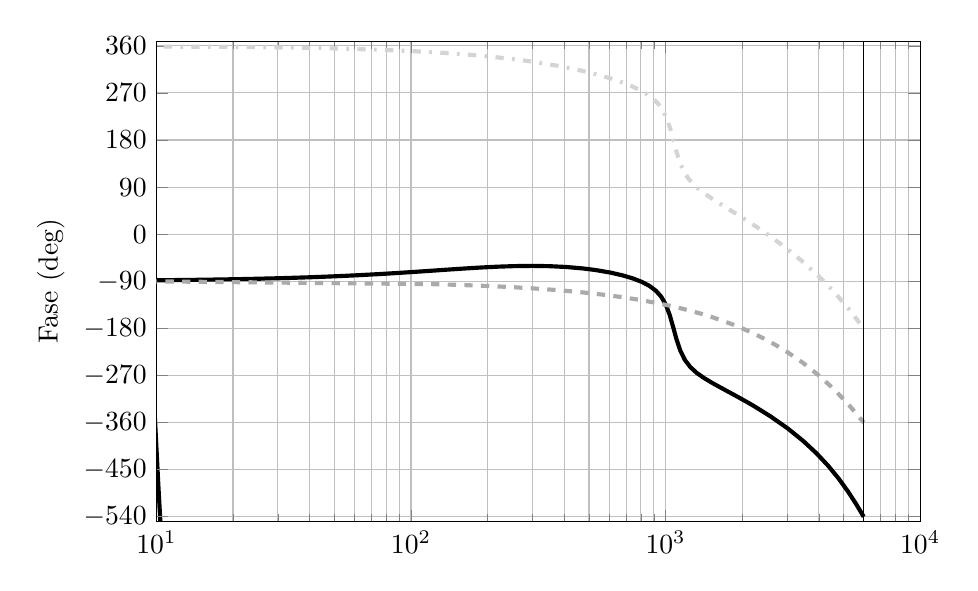
\begin{tikzpicture}

\begin{axis}[%
width=0.8\textwidth,
height=0.256994536928635\textwidth,
unbounded coords=jump,
scale only axis,
xmode=log,
xmin=10,
xmax=10000,
xtick={10,100,1000,10000},
xticklabels={\empty},
xminorticks=true,
xmajorgrids,
xminorgrids,
ymin=0,
ymax=1,
ylabel={Magnitude (dB)},
ymajorgrids,
hide axis
]
\addplot [color=black,solid,line width=1.5pt,forget plot]
  table[row sep=crcr]{9.14152673182037	1.1\\
10.1733925633752	0.151765865562977\\
10.493143807408	-0.1\\
};
\addplot [color=black,solid,forget plot]
  table[row sep=crcr]{6000	-0.100000000000001\\
6000	0\\
6000	1.10000000000001\\
};
\addplot [color=mycolor1,dashed,line width=1.5pt,forget plot]
  table[row sep=crcr]{11.2668826135566	1.1\\
nan	nan\\
11.6232827408475	-0.1\\
};
\addplot [color=black,solid,forget plot]
  table[row sep=crcr]{6000	-0.100000000000001\\
6000	0\\
6000	1.10000000000001\\
};
\addplot [color=white!50!mycolor1,dash pattern=on 1pt off 3pt on 3pt off 3pt,line width=1.5pt,forget plot]
  table[row sep=crcr]{9511.2091450406	-0.100000000000001\\
nan	nan\\
9511.2091450406	-0.100000000000001\\
nan	nan\\
8203.14101765779	-0.100000000000001\\
nan	nan\\
8203.14101765779	-0.100000000000001\\
nan	nan\\
7051.72917006881	-0.100000000000001\\
nan	nan\\
7051.72917006881	-0.100000000000001\\
nan	nan\\
6036.25309350788	-0.100000000000001\\
nan	nan\\
6036.25309350788	-0.100000000000001\\
nan	nan\\
5138.95637184777	-0.100000000000001\\
nan	nan\\
5138.95637184777	-0.100000000000001\\
nan	nan\\
4344.85349477849	-0.100000000000001\\
nan	nan\\
4344.85349477849	-0.100000000000001\\
nan	nan\\
3641.63180316766	-0.0999999999999979\\
nan	nan\\
3641.63180316766	-0.0999999999999979\\
nan	nan\\
3152.6813160531	-0.100000000000001\\
nan	nan\\
3152.6813160531	-0.100000000000001\\
nan	nan\\
2739.67953214222	-0.100000000000005\\
nan	nan\\
2739.67953214222	-0.100000000000005\\
nan	nan\\
2340.89883883785	-0.100000000000001\\
nan	nan\\
2340.89883883785	-0.100000000000001\\
nan	nan\\
2031.17443534533	-0.100000000000001\\
nan	nan\\
2031.17443534533	-0.100000000000001\\
nan	nan\\
1790.97315445953	-0.100000000000005\\
nan	nan\\
1790.97315445953	-0.100000000000005\\
nan	nan\\
1606.48399968917	-0.100000000000001\\
nan	nan\\
1606.48399968917	-0.100000000000001\\
nan	nan\\
1468.08732614798	-0.100000000000001\\
nan	nan\\
1468.08732614798	-0.100000000000001\\
nan	nan\\
1369.66985403292	-0.100000000000001\\
nan	nan\\
1369.66985403292	-0.100000000000001\\
nan	nan\\
1309.03750327975	-0.100000000000001\\
nan	nan\\
1309.03750327975	-0.0999999999999996\\
nan	nan\\
1291.40601147537	-0.100000000000001\\
nan	nan\\
1291.40601147537	-0.0999999999999996\\
nan	nan\\
1349.85706933905	-0.0999999999999996\\
nan	nan\\
1349.85706933905	-0.0999999999999996\\
nan	nan\\
1830.00209838628	-0.100000000000001\\
nan	nan\\
1830.00209838628	-0.100000000000001\\
nan	nan\\
428.198837526225	-0.100000000000001\\
nan	nan\\
428.198837526225	-0.100000000000001\\
nan	nan\\
834.234890057516	-0.0999999999999979\\
nan	nan\\
834.234890057516	-0.0999999999999996\\
nan	nan\\
888.615601373851	-0.0999999999999996\\
nan	nan\\
888.615601373851	-0.0999999999999996\\
nan	nan\\
869.314096520499	-0.100000000000001\\
nan	nan\\
869.314096520499	-0.100000000000005\\
nan	nan\\
803.599512020507	-0.100000000000001\\
nan	nan\\
803.599512020507	-0.100000000000005\\
nan	nan\\
693.623933765194	-0.0999999999999979\\
nan	nan\\
693.623933765194	-0.0999999999999979\\
nan	nan\\
533.51559945153	-0.100000000000001\\
nan	nan\\
533.51559945153	-0.100000000000001\\
nan	nan\\
311.132819462156	-0.100000000000001\\
nan	nan\\
311.132819462156	-0.100000000000001\\
nan	nan\\
5.9286831368604	-0.100000000000001\\
nan	nan\\
5.9286831368604	-0.100000000000001\\
nan	nan\\
-416.700333620808	-0.100000000000001\\
nan	nan\\
-416.700333620808	-0.100000000000001\\
};
\addplot [color=black,solid,forget plot]
  table[row sep=crcr]{6000	-0.100000000000001\\
6000	0\\
6000	1.10000000000001\\
};
\end{axis}

\begin{axis}[%
width=0.8\textwidth,
height=0.503129594988472\textwidth,
scale only axis,
xmode=log,
xmin=10,
xmax=10000,
xminorticks=true,
xmajorgrids,
xminorgrids,
ymin=-549,
ymax=369,
ytick={-540, -450, -360, -270, -180,  -90,    0,   90,  180,  270,  360},
ylabel={Fase (deg)},
ymajorgrids
]
\addplot [color=black,solid,line width=1.5pt,forget plot]
  table[row sep=crcr]{8.72405426743874	-88.2938615386012\\
10.1733925633752	-88.0110701481703\\
11.8635112845217	-87.6816789542002\\
13.8344115909431	-87.2981681364625\\
16.1327400865988	-86.8518972552513\\
18.812892835438	-86.3329929524079\\
21.938302789101	-85.7302595705756\\
25.5829410966331	-85.0311389460326\\
29.8330678286992	-84.2217610456517\\
34.7892735518555	-83.2871493435661\\
40.5688600721623	-82.2116752697912\\
47.3086166947834	-80.979894550798\\
55.1680577071395	-79.5779404900146\\
64.3331977092853	-77.9956822801232\\
75.0209541447453	-76.2298527195457\\
87.4842812294358	-74.2882624869803\\
102.01815678676	-72.1949875372793\\
118.966563683284	-69.9960015271512\\
138.730631099244	-67.7641756520263\\
161.778128318745	-65.6021078418664\\
188.654535735468	-63.6412718501436\\
219.995955098717	-62.0368570964678\\
256.544164555156	-60.9593357342465\\
299.1641748039	-60.5855602545681\\
348.864701878087	-61.0932261378975\\
406.822041095882	-62.6628300973953\\
474.40790722145	-65.4925994237857\\
531.504182204689	-68.5416909427112\\
606.064869421581	-73.2980007853734\\
677.501516549994	-78.6723563862003\\
744.70428505611	-84.6102766854428\\
806.949577729217	-91.2145470387639\\
863.84758836883	-98.7824823445223\\
915.278419070289	-107.881418119299\\
961.327424257804	-119.451905412323\\
1002.22625276946	-134.766635697479\\
1038.30279972218	-154.552040486626\\
1069.94103119274	-176.761083830538\\
1102.54331447059	-200.110286680467\\
1142.23091549082	-222.50485764839\\
1190.82612369414	-240.312294522124\\
1250.73833969845	-253.940929717949\\
1325.20345677115	-265.077270053466\\
1418.64354579777	-275.151757278749\\
1537.21931403086	-285.227785828359\\
1689.69925862198	-296.188075724093\\
1888.86349958272	-308.918320610209\\
2153.83782208684	-324.490156202513\\
2206.10594744096	-327.449317253119\\
2572.60915071119	-347.576159036155\\
3000	-370.287544142107\\
3030.2689591777	-371.882234900294\\
3469.23953517283	-394.997515408547\\
3912.38254234155	-418.601633069524\\
4353.43031613188	-442.704449480924\\
4786.88753737426	-467.214847370754\\
5208.13303270343	-491.892653946513\\
5613.4498161518	-516.328305734671\\
6000	-540\\
};
\addplot [color=black,solid,forget plot]
  table[row sep=crcr]{6000	-640.8\\
6000	-1\\
6000	0\\
6000	1\\
6000	460.8\\
};
\addplot [color=mycolor1,dashed,line width=1.5pt,forget plot]
  table[row sep=crcr]{0.12	-90.0054\\
12	-90.54\\
120	-95.4\\
132.294888466487	-95.9532699809919\\
145.849479286335	-96.5632265678851\\
160.79283829234	-97.2356777231553\\
177.267255067459	-97.9770264780356\\
195.429597815914	-98.7943319017161\\
215.45280705089	-99.69537631729\\
237.527542321575	-100.688739404471\\
261.863997659596	-101.783879894682\\
288.693903031372	-102.991225636412\\
318.272730854084	-104.322272888434\\
350.882128585544	-105.789695786349\\
386.8326005509	-107.407467024791\\
426.466464542353	-109.190990904406\\
470.161111344397	-111.157250010498\\
518.332598221554	-113.32496691997\\
571.43961058554	-115.714782476349\\
629.987829564556	-118.349452330405\\
694.534747062392	-121.254063617808\\
765.69497415599	-124.45627383702\\
844.146093377636	-127.986574201994\\
930.63511060679	-131.878579977306\\
1025.98556800602	-136.169350560271\\
1131.10538572984	-140.899742357843\\
1246.99550707477	-146.114797818365\\
1374.75942938889	-151.8641743225\\
1515.61371149379	-158.20261701722\\
1670.89955766957	-165.190480095131\\
1842.09558850499	-172.894301482724\\
2030.83192021562	-181.387436409703\\
2238.90568649256	-190.750755892165\\
2468.2981506793	-201.073416780568\\
2721.19357121795	-212.453710704808\\
3000	-225\\
3446.0950649911	-245.074277924599\\
3958.52373231868	-268.133567954341\\
4547.14969953119	-294.621736478903\\
5223.30337977675	-325.048652089954\\
6000	-360\\
};
\addplot [color=black,solid,forget plot]
  table[row sep=crcr]{6000	-640.8\\
6000	-1\\
6000	0\\
6000	1\\
6000	460.8\\
};
\addplot [color=white!50!mycolor1,dash pattern=on 1pt off 3pt on 3pt off 3pt,line width=1.5pt,forget plot]
  table[row sep=crcr]{2.15231873701794	359.782330906982\\
21.5231873701794	357.823313260247\\
24.6869879475792	357.50335274276\\
28.3158513393938	357.136360389991\\
32.4781394464639	356.715423127939\\
37.2522630261321	356.232611869039\\
42.7281588237413	355.678832237219\\
49.0089838350534	355.043653373679\\
56.2130586167442	354.315111599165\\
64.4760962537936	353.479485219446\\
73.9537589739008	352.521036178081\\
84.8245905713938	351.421713545549\\
97.2933798827434	350.160812914832\\
111.595018676107	348.714584512763\\
127.998926631282	347.05578096071\\
146.814126769514	345.15313257591\\
168.395066946031	342.970732763619\\
193.148297072777	340.46730605158\\
221.540127859386	337.5953116608\\
254.105415350673	334.299795345049\\
291.45763674706	330.516817324008\\
334.300447320066	326.171098016628\\
383.440936136402	321.172096878756\\
439.804830307013	315.406703822974\\
504.453934184461	308.723995921324\\
546.926133466315	304.269684566912\\
612.995741548141	297.179449533476\\
676.484836199587	290.071217245074\\
736.621653800288	282.889406143951\\
792.878286667478	275.501359069167\\
844.941663795275	267.672492459216\\
892.678131956279	259.024260765399\\
936.096724379532	248.973181372028\\
975.314466440107	236.685862363572\\
1010.52563749564	221.231816307449\\
1041.97584345845	202.391925236669\\
1069.94103119273	182.032393772687\\
1098.65676581342	160.764197375888\\
1132.84984344072	139.700914637596\\
1173.74841614745	121.939503201633\\
1222.92256816575	107.748964630919\\
1282.40377942386	96.008575334702\\
1354.85544065577	85.5518273516384\\
1443.8203561373	75.4724032029015\\
1554.0865576294	65.061338341509\\
1692.23868588241	53.6987464341057\\
1867.5069541896	40.759922505689\\
2093.10497374555	25.5264869518217\\
2280.33271317212	13.6751727231532\\
2615.5301832547	-6.33972481291113\\
3000	-27.9979210745996\\
3446.0950649911	-51.987179676834\\
3958.52373231868	-78.5654347600015\\
4547.14969953119	-108.292891072803\\
5223.30337977675	-141.833364854922\\
6000	-180\\
};
\addplot [color=black,solid,forget plot]
  table[row sep=crcr]{6000	-640.8\\
6000	-1\\
6000	0\\
6000	1\\
6000	460.8\\
};
\end{axis}
\end{tikzpicture}%}}\\
  %   \subfloat[Diagrama de pólos e zeros para $\Delta(z)$.]{\label{fig:pzmap_delta_vc}
  %     {\def\svgwidth{0.8\textwidth}% This file was created by matlab2tikz v0.4.7 running on MATLAB 8.3.
% Copyright (c) 2008--2014, Nico Schlömer <nico.schloemer@gmail.com>
% All rights reserved.
% Minimal pgfplots version: 1.3
% 
% The latest updates can be retrieved from
%   http://www.mathworks.com/matlabcentral/fileexchange/22022-matlab2tikz
% where you can also make suggestions and rate matlab2tikz.
% 
%
% defining custom colors
\definecolor{mycolor1}{rgb}{0.66667,0.66667,0.66667}%
%
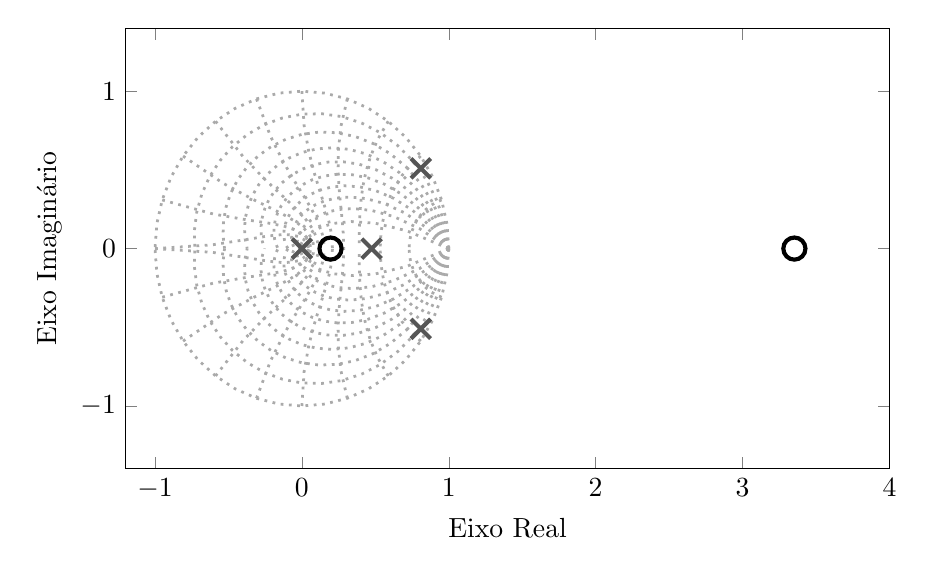
\begin{tikzpicture}

\begin{axis}[%
width=0.8\textwidth,
height=0.461611624834875\textwidth,
scale only axis,
xmin=-1.2,
xmax=4,
xtick={-1,  0,  1,  2,  3,  4},
xlabel={Eixo Real},
ymin=-1.4,
ymax=1.4,
ytick={-1,  0,  1},
ylabel={Eixo Imaginário}
]
\addplot [color=mycolor1,dotted,line width=1.0pt,forget plot]
  table[row sep=crcr]{1	0\\
0.987688340595138	0.156434465040231\\
0.951056516295154	0.309016994374947\\
0.891006524188368	0.453990499739547\\
0.809016994374947	0.587785252292473\\
0.707106781186548	0.707106781186547\\
0.587785252292473	0.809016994374947\\
0.453990499739547	0.891006524188368\\
0.309016994374947	0.951056516295154\\
0.156434465040231	0.987688340595138\\
6.12323399573677e-17	1\\
-0.156434465040231	0.987688340595138\\
-0.309016994374947	0.951056516295154\\
-0.453990499739547	0.891006524188368\\
-0.587785252292473	0.809016994374947\\
-0.707106781186547	0.707106781186548\\
-0.809016994374947	0.587785252292473\\
-0.891006524188368	0.453990499739547\\
-0.951056516295154	0.309016994374948\\
-0.987688340595138	0.156434465040231\\
-1	1.22464679914735e-16\\
};
\addplot [color=mycolor1,dotted,line width=1.0pt,forget plot]
  table[row sep=crcr]{1	0\\
0.972218045703082	0.153984211042097\\
0.921496791140463	0.299412457456957\\
0.849791018366557	0.432990150609548\\
0.759508516401756	0.551815237548133\\
0.653437051516106	0.653437051516106\\
0.534664304371591	0.735902282058355\\
0.406492952796512	0.797787339572243\\
0.272353130096494	0.83821674479613\\
0.135714483753824	0.856867527364047\\
5.22899666167123e-17	0.853959960588124\\
-0.131496350792703	0.830235283991667\\
-0.255686250369537	0.786921363444393\\
-0.369756251949576	0.725687504552447\\
-0.47122811850853	0.648589862732789\\
-0.558009078759514	0.558009078759514\\
-0.628431083783263	0.456581908289041\\
-0.681278445058817	0.347128705949459\\
-0.715803538350409	0.232578668243255\\
-0.731730559897045	0.115894735197653\\
-0.729247614287671	8.9307075662324e-17\\
};
\addplot [color=mycolor1,dotted,line width=1.0pt,forget plot]
  table[row sep=crcr]{1	0\\
0.956521682769877	0.151498151383791\\
0.891982039736211	0.289822533396298\\
0.809292583610082	0.412355167436434\\
0.711634858347723	0.517032989000692\\
0.602364630186427	0.602364630186426\\
0.484917701774751	0.667431957639199\\
0.362719588349683	0.711877274647591\\
0.239101059900595	0.735877395777214\\
0.117221283062812	0.740106053489981\\
4.44354699422903e-17	0.725686295399261\\
-0.109940132237539	0.694134676438339\\
-0.210320240583588	0.647299141978847\\
-0.299240493845688	0.587292536894097\\
-0.375203754387119	0.516423664031337\\
-0.437127756959533	0.437127756959533\\
-0.484346224770267	0.351898130574443\\
-0.516599582217932	0.263220634338226\\
-0.534016141209622	0.173512362385299\\
-0.537084820159711	0.0850658786478001\\
-0.526620599330303	6.44924231334916e-17\\
};
\addplot [color=mycolor1,dotted,line width=1.0pt,forget plot]
  table[row sep=crcr]{1	0\\
0.940082788364644	0.148894486293864\\
0.86158608093073	0.279946287694513\\
0.768279786681378	0.391458103646313\\
0.663960650859636	0.482395649771645\\
0.552351927561387	0.552351927561387\\
0.437014383712816	0.601498696728173\\
0.321269860940431	0.630527604183869\\
0.208138182971344	0.640583459188477\\
0.100287778328637	0.633192112325829\\
3.73630739569174e-17	0.610185303761559\\
-0.0908532273476425	0.573624701779294\\
-0.170819110593797	0.525727164509449\\
-0.238861981883349	0.468793035010043\\
-0.294350736089166	0.40513903143051\\
-0.337037028702328	0.337037028702328\\
-0.367025664975262	0.266659754473976\\
-0.384738677688982	0.196034147687371\\
-0.390874612629551	0.127002860400749\\
-0.386364521398959	0.0611941284830315\\
-0.372326104926586	4.55967972637346e-17\\
};
\addplot [color=mycolor1,dotted,line width=1.0pt,forget plot]
  table[row sep=crcr]{1	0\\
0.922246029428501	0.146069421212559\\
0.829201462983264	0.269423887468404\\
0.725373165529273	0.369596088217499\\
0.614985835074999	0.446813363302878\\
0.501902475185001	0.501902475185001\\
0.38956496084428	0.536190168955128\\
0.280953750703967	0.551402782692681\\
0.178565395716864	0.549567778706978\\
0.0844061798404073	0.532919645815306\\
3.08495992433718e-17	0.50381218919366\\
-0.0735915548753502	0.464638791061534\\
-0.135739038566523	0.417761804348184\\
-0.186207014322272	0.365451842507638\\
-0.225110018726605	0.309837359892227\\
-0.252864584784672	0.252864584784672\\
-0.270139142845401	0.196267575756099\\
-0.277803443075876	0.141547924204336\\
-0.27687894570066	0.0899634229303457\\
-0.268491413422519	0.0425248622468694\\
-0.253826721980109	3.10848082611005e-17\\
};
\addplot [color=mycolor1,dotted,line width=1.0pt,forget plot]
  table[row sep=crcr]{1	0\\
0.902056570675584	0.142871725087523\\
0.793293726869509	0.257756756757911\\
0.678769666307395	0.345850419328459\\
0.562876391436159	0.408953636388562\\
0.449318435861499	0.449318435861499\\
0.341115747349381	0.469505547439701\\
0.24062663375655	0.472256359314945\\
0.149586755320764	0.460380694230177\\
0.069160331541479	0.436661148025441\\
2.47240337905553e-17	0.403774113610049\\
-0.057687904157153	0.364227092250654\\
-0.104075505986926	0.320311471399148\\
-0.139645446506012	0.274069620358657\\
-0.165124892040398	0.227274916024158\\
-0.18142315316863	0.18142315316863\\
-0.189574186252466	0.137733708524426\\
-0.190684892879101	0.0971588057560207\\
-0.185889806735969	0.0603992595374446\\
-0.176312467991919	0.0279251515651378\\
-0.16303353482158	1.99658496572927e-17\\
};
\addplot [color=mycolor1,dotted,line width=1.0pt,forget plot]
  table[row sep=crcr]{1	0\\
0.877921760602431	0.139049146701748\\
0.751411952540787	0.244148543365328\\
0.625732257688895	0.318826509862098\\
0.505011411193747	0.36691226736026\\
0.392341669548685	0.392341669548685\\
0.289890514921595	0.399000063654162\\
0.199020572856858	0.390599867100522\\
0.120411913496453	0.370589763847805\\
0.0541820486548744	0.34209199176291\\
1.88512313530119e-17	0.307863971328499\\
-0.042808222513439	0.270280479734772\\
-0.075164540154518	0.231332667812908\\
-0.0981551954909503	0.192640417840451\\
-0.112959067758674	0.155474818616317\\
-0.120787864504912	0.120787864504912\\
-0.122837744156894	0.0892468451742257\\
-0.120251626285951	0.0612712639357851\\
-0.114091236431876	0.0370704898842818\\
-0.105317799143806	0.0166807006736036\\
-0.0947802248421549	1.16072298975411e-17\\
};
\addplot [color=mycolor1,dotted,line width=1.0pt,forget plot]
  table[row sep=crcr]{1	0\\
0.84674396664984	0.134111069256013\\
0.698989566160914	0.227115477506975\\
0.561406498364893	0.286050898428465\\
0.437004973478602	0.317502698182059\\
0.327450698344114	0.327450698344114\\
0.233352139914598	0.321181666481713\\
0.154515499860225	0.303253743289057\\
0.0901653834921457	0.27750051639687\\
0.0391311034995635	0.247064063991275\\
1.31311479217367e-17	0.214447919692096\\
-0.0287598398096346	0.181582482159892\\
-0.0487044416812479	0.149896858349689\\
-0.0613430200940395	0.120392455675976\\
-0.06808779312177	0.0937148074575858\\
-0.0702211210616195	0.0702211210616195\\
-0.068876740220244	0.0500418809603846\\
-0.0650321343871793	0.0331355275052096\\
-0.0595094084547913	0.0193357789181307\\
-0.0529823745536039	0.00839158374073751\\
-0.0459879102602678	5.63189470997126e-18\\
};
\addplot [color=mycolor1,dotted,line width=1.0pt,forget plot]
  table[row sep=crcr]{1	0\\
0.801053465278425	0.126874404768154\\
0.625589539649299	0.203266363189334\\
0.475341369738971	0.242198525079547\\
0.350045057714404	0.254322621147605\\
0.24813777530853	0.24813777530853\\
0.167289292234614	0.230253957320141\\
0.104794333468008	0.205670459781722\\
0.0578515468028918	0.178048753195384\\
0.0237523524567972	0.149966451301199\\
7.54043881219821e-18	0.123144711070133\\
-0.0156239119173694	0.0986454975334405\\
-0.0250311775652273	0.0770380431086105\\
-0.0298254673925332	0.0585357756361869\\
-0.0313184856998208	0.0431061974937683\\
-0.0305568546459545	0.0305568546459545\\
-0.0283545570469435	0.0206007915573586\\
-0.0253272293454815	0.012904867916705\\
-0.021925762268643	0.00712411201600239\\
-0.0184675753156993	0.00292497658052826\\
-0.0151646198645466	1.85713031774033e-18\\
};
\addplot [color=mycolor1,dotted,line width=1.0pt,forget plot]
  table[row sep=crcr]{1	0\\
0.714110955679367	0.113104064044896\\
0.497161927717827	0.161537702532642\\
0.336758208677056	0.171586877647116\\
0.221075553032581	0.160620791180475\\
0.139705610200823	0.139705610200823\\
0.0839640345306934	0.115566579097864\\
0.0468885871776745	0.0920240337831981\\
0.0230753615892199	0.0710186604775083\\
0.00844586939409394	0.0533251206797082\\
2.39022368106624e-18	0.0390353150431684\\
-0.00441505277265522	0.0278755461307222\\
-0.00630567510971132	0.0194068724759343\\
-0.00669794782622876	0.0131454627690819\\
-0.0062698831862128	0.00862975386096949\\
-0.0054534525074872	0.0054534525074872\\
-0.00451117782354635	0.00327756254020109\\
-0.00359218715027031	0.00183031077240959\\
-0.00277223578568335	0.000900754009370227\\
-0.00208156288544739	0.000329687172611911\\
-0.00152375582051941	1.86606268828125e-19\\
};
\addplot [color=mycolor1,dotted,line width=1.0pt,forget plot]
  table[row sep=crcr]{1	-0\\
0.987688340595138	-0.156434465040231\\
0.951056516295154	-0.309016994374947\\
0.891006524188368	-0.453990499739547\\
0.809016994374947	-0.587785252292473\\
0.707106781186548	-0.707106781186547\\
0.587785252292473	-0.809016994374947\\
0.453990499739547	-0.891006524188368\\
0.309016994374947	-0.951056516295154\\
0.156434465040231	-0.987688340595138\\
6.12323399573677e-17	-1\\
-0.156434465040231	-0.987688340595138\\
-0.309016994374947	-0.951056516295154\\
-0.453990499739547	-0.891006524188368\\
-0.587785252292473	-0.809016994374947\\
-0.707106781186547	-0.707106781186548\\
-0.809016994374947	-0.587785252292473\\
-0.891006524188368	-0.453990499739547\\
-0.951056516295154	-0.309016994374948\\
-0.987688340595138	-0.156434465040231\\
-1	-1.22464679914735e-16\\
};
\addplot [color=mycolor1,dotted,line width=1.0pt,forget plot]
  table[row sep=crcr]{1	-0\\
0.972218045703082	-0.153984211042097\\
0.921496791140463	-0.299412457456957\\
0.849791018366557	-0.432990150609548\\
0.759508516401756	-0.551815237548133\\
0.653437051516106	-0.653437051516106\\
0.534664304371591	-0.735902282058355\\
0.406492952796512	-0.797787339572243\\
0.272353130096494	-0.83821674479613\\
0.135714483753824	-0.856867527364047\\
5.22899666167123e-17	-0.853959960588124\\
-0.131496350792703	-0.830235283991667\\
-0.255686250369537	-0.786921363444393\\
-0.369756251949576	-0.725687504552447\\
-0.47122811850853	-0.648589862732789\\
-0.558009078759514	-0.558009078759514\\
-0.628431083783263	-0.456581908289041\\
-0.681278445058817	-0.347128705949459\\
-0.715803538350409	-0.232578668243255\\
-0.731730559897045	-0.115894735197653\\
-0.729247614287671	-8.9307075662324e-17\\
};
\addplot [color=mycolor1,dotted,line width=1.0pt,forget plot]
  table[row sep=crcr]{1	-0\\
0.956521682769877	-0.151498151383791\\
0.891982039736211	-0.289822533396298\\
0.809292583610082	-0.412355167436434\\
0.711634858347723	-0.517032989000692\\
0.602364630186427	-0.602364630186426\\
0.484917701774751	-0.667431957639199\\
0.362719588349683	-0.711877274647591\\
0.239101059900595	-0.735877395777214\\
0.117221283062812	-0.740106053489981\\
4.44354699422903e-17	-0.725686295399261\\
-0.109940132237539	-0.694134676438339\\
-0.210320240583588	-0.647299141978847\\
-0.299240493845688	-0.587292536894097\\
-0.375203754387119	-0.516423664031337\\
-0.437127756959533	-0.437127756959533\\
-0.484346224770267	-0.351898130574443\\
-0.516599582217932	-0.263220634338226\\
-0.534016141209622	-0.173512362385299\\
-0.537084820159711	-0.0850658786478001\\
-0.526620599330303	-6.44924231334916e-17\\
};
\addplot [color=mycolor1,dotted,line width=1.0pt,forget plot]
  table[row sep=crcr]{1	-0\\
0.940082788364644	-0.148894486293864\\
0.86158608093073	-0.279946287694513\\
0.768279786681378	-0.391458103646313\\
0.663960650859636	-0.482395649771645\\
0.552351927561387	-0.552351927561387\\
0.437014383712816	-0.601498696728173\\
0.321269860940431	-0.630527604183869\\
0.208138182971344	-0.640583459188477\\
0.100287778328637	-0.633192112325829\\
3.73630739569174e-17	-0.610185303761559\\
-0.0908532273476425	-0.573624701779294\\
-0.170819110593797	-0.525727164509449\\
-0.238861981883349	-0.468793035010043\\
-0.294350736089166	-0.40513903143051\\
-0.337037028702328	-0.337037028702328\\
-0.367025664975262	-0.266659754473976\\
-0.384738677688982	-0.196034147687371\\
-0.390874612629551	-0.127002860400749\\
-0.386364521398959	-0.0611941284830315\\
-0.372326104926586	-4.55967972637346e-17\\
};
\addplot [color=mycolor1,dotted,line width=1.0pt,forget plot]
  table[row sep=crcr]{1	-0\\
0.922246029428501	-0.146069421212559\\
0.829201462983264	-0.269423887468404\\
0.725373165529273	-0.369596088217499\\
0.614985835074999	-0.446813363302878\\
0.501902475185001	-0.501902475185001\\
0.38956496084428	-0.536190168955128\\
0.280953750703967	-0.551402782692681\\
0.178565395716864	-0.549567778706978\\
0.0844061798404073	-0.532919645815306\\
3.08495992433718e-17	-0.50381218919366\\
-0.0735915548753502	-0.464638791061534\\
-0.135739038566523	-0.417761804348184\\
-0.186207014322272	-0.365451842507638\\
-0.225110018726605	-0.309837359892227\\
-0.252864584784672	-0.252864584784672\\
-0.270139142845401	-0.196267575756099\\
-0.277803443075876	-0.141547924204336\\
-0.27687894570066	-0.0899634229303457\\
-0.268491413422519	-0.0425248622468694\\
-0.253826721980109	-3.10848082611005e-17\\
};
\addplot [color=mycolor1,dotted,line width=1.0pt,forget plot]
  table[row sep=crcr]{1	-0\\
0.902056570675584	-0.142871725087523\\
0.793293726869509	-0.257756756757911\\
0.678769666307395	-0.345850419328459\\
0.562876391436159	-0.408953636388562\\
0.449318435861499	-0.449318435861499\\
0.341115747349381	-0.469505547439701\\
0.24062663375655	-0.472256359314945\\
0.149586755320764	-0.460380694230177\\
0.069160331541479	-0.436661148025441\\
2.47240337905553e-17	-0.403774113610049\\
-0.057687904157153	-0.364227092250654\\
-0.104075505986926	-0.320311471399148\\
-0.139645446506012	-0.274069620358657\\
-0.165124892040398	-0.227274916024158\\
-0.18142315316863	-0.18142315316863\\
-0.189574186252466	-0.137733708524426\\
-0.190684892879101	-0.0971588057560207\\
-0.185889806735969	-0.0603992595374446\\
-0.176312467991919	-0.0279251515651378\\
-0.16303353482158	-1.99658496572927e-17\\
};
\addplot [color=mycolor1,dotted,line width=1.0pt,forget plot]
  table[row sep=crcr]{1	-0\\
0.877921760602431	-0.139049146701748\\
0.751411952540787	-0.244148543365328\\
0.625732257688895	-0.318826509862098\\
0.505011411193747	-0.36691226736026\\
0.392341669548685	-0.392341669548685\\
0.289890514921595	-0.399000063654162\\
0.199020572856858	-0.390599867100522\\
0.120411913496453	-0.370589763847805\\
0.0541820486548744	-0.34209199176291\\
1.88512313530119e-17	-0.307863971328499\\
-0.042808222513439	-0.270280479734772\\
-0.075164540154518	-0.231332667812908\\
-0.0981551954909503	-0.192640417840451\\
-0.112959067758674	-0.155474818616317\\
-0.120787864504912	-0.120787864504912\\
-0.122837744156894	-0.0892468451742257\\
-0.120251626285951	-0.0612712639357851\\
-0.114091236431876	-0.0370704898842818\\
-0.105317799143806	-0.0166807006736036\\
-0.0947802248421549	-1.16072298975411e-17\\
};
\addplot [color=mycolor1,dotted,line width=1.0pt,forget plot]
  table[row sep=crcr]{1	-0\\
0.84674396664984	-0.134111069256013\\
0.698989566160914	-0.227115477506975\\
0.561406498364893	-0.286050898428465\\
0.437004973478602	-0.317502698182059\\
0.327450698344114	-0.327450698344114\\
0.233352139914598	-0.321181666481713\\
0.154515499860225	-0.303253743289057\\
0.0901653834921457	-0.27750051639687\\
0.0391311034995635	-0.247064063991275\\
1.31311479217367e-17	-0.214447919692096\\
-0.0287598398096346	-0.181582482159892\\
-0.0487044416812479	-0.149896858349689\\
-0.0613430200940395	-0.120392455675976\\
-0.06808779312177	-0.0937148074575858\\
-0.0702211210616195	-0.0702211210616195\\
-0.068876740220244	-0.0500418809603846\\
-0.0650321343871793	-0.0331355275052096\\
-0.0595094084547913	-0.0193357789181307\\
-0.0529823745536039	-0.00839158374073751\\
-0.0459879102602678	-5.63189470997126e-18\\
};
\addplot [color=mycolor1,dotted,line width=1.0pt,forget plot]
  table[row sep=crcr]{1	-0\\
0.801053465278425	-0.126874404768154\\
0.625589539649299	-0.203266363189334\\
0.475341369738971	-0.242198525079547\\
0.350045057714404	-0.254322621147605\\
0.24813777530853	-0.24813777530853\\
0.167289292234614	-0.230253957320141\\
0.104794333468008	-0.205670459781722\\
0.0578515468028918	-0.178048753195384\\
0.0237523524567972	-0.149966451301199\\
7.54043881219821e-18	-0.123144711070133\\
-0.0156239119173694	-0.0986454975334405\\
-0.0250311775652273	-0.0770380431086105\\
-0.0298254673925332	-0.0585357756361869\\
-0.0313184856998208	-0.0431061974937683\\
-0.0305568546459545	-0.0305568546459545\\
-0.0283545570469435	-0.0206007915573586\\
-0.0253272293454815	-0.012904867916705\\
-0.021925762268643	-0.00712411201600239\\
-0.0184675753156993	-0.00292497658052826\\
-0.0151646198645466	-1.85713031774033e-18\\
};
\addplot [color=mycolor1,dotted,line width=1.0pt,forget plot]
  table[row sep=crcr]{1	-0\\
0.714110955679367	-0.113104064044896\\
0.497161927717827	-0.161537702532642\\
0.336758208677056	-0.171586877647116\\
0.221075553032581	-0.160620791180475\\
0.139705610200823	-0.139705610200823\\
0.0839640345306934	-0.115566579097864\\
0.0468885871776745	-0.0920240337831981\\
0.0230753615892199	-0.0710186604775083\\
0.00844586939409394	-0.0533251206797082\\
2.39022368106624e-18	-0.0390353150431684\\
-0.00441505277265522	-0.0278755461307222\\
-0.00630567510971132	-0.0194068724759343\\
-0.00669794782622876	-0.0131454627690819\\
-0.0062698831862128	-0.00862975386096949\\
-0.0054534525074872	-0.0054534525074872\\
-0.00451117782354635	-0.00327756254020109\\
-0.00359218715027031	-0.00183031077240959\\
-0.00277223578568335	-0.000900754009370227\\
-0.00208156288544739	-0.000329687172611911\\
-0.00152375582051941	-1.86606268828125e-19\\
};
\addplot [color=mycolor1,dotted,line width=1.0pt,forget plot]
  table[row sep=crcr]{1	0\\
1	0\\
};
\addplot [color=mycolor1,dotted,line width=1.0pt,forget plot]
  table[row sep=crcr]{0.951056516295154	0.309016994374947\\
0.906577591518048	0.290693092532446\\
0.867277205719189	0.267124444629623\\
0.833330533437629	0.239553777474139\\
0.804679893747523	0.20903820245934\\
0.781122098933164	0.176433510213537\\
0.762382187756933	0.142402376999381\\
0.748171074803624	0.107437628337747\\
0.738227708485823	0.0718935522249012\\
0.732347931289196	0.0360204899377399\\
0.730402691048646	2.81010850277162e-17\\
};
\addplot [color=mycolor1,dotted,line width=1.0pt,forget plot]
  table[row sep=crcr]{0.809016994374947	0.587785252292473\\
0.737380455396588	0.527071687397996\\
0.6808142826414	0.463341883835339\\
0.637053765657314	0.399254954339046\\
0.603812761314093	0.336417677088311\\
0.579022949915482	0.275632227640288\\
0.560948163233974	0.217130071437151\\
0.54821711318997	0.160763451735608\\
0.539811466724715	0.106147624627789\\
0.535036016768209	0.0527590625798542\\
0.533488091091103	4.10502162512614e-17\\
};
\addplot [color=mycolor1,dotted,line width=1.0pt,forget plot]
  table[row sep=crcr]{0.587785252292473	0.809016994374947\\
0.515276498489902	0.692182785870847\\
0.46668476526979	0.583707991451876\\
0.435233321876477	0.485319980094308\\
0.415551842123536	0.396928474901319\\
0.403656860517901	0.317461475735791\\
0.396737049613855	0.245416450708029\\
0.392888142823216	0.179177710929467\\
0.39087245229983	0.11717008156476\\
0.389932112762627	0.0579102497954412\\
0.389661137375347	4.49747826270753e-17\\
};
\addplot [color=mycolor1,dotted,line width=1.0pt,forget plot]
  table[row sep=crcr]{0.309016994374947	0.951056516295154\\
0.265925372344309	0.777304721760365\\
0.248822386132444	0.630899544522142\\
0.24643298177389	0.508693744238057\\
0.251412997268255	0.406266573115132\\
0.25929445161488	0.31919477108011\\
0.267517373913267	0.243597429511063\\
0.274697115780397	0.1762665508339\\
0.280129101393366	0.114599409879343\\
0.283480020554887	0.0564559973822998\\
0.284609543336029	4.37996030135249e-17\\
};
\addplot [color=mycolor1,dotted,line width=1.0pt,forget plot]
  table[row sep=crcr]{6.12323399573677e-17	1\\
0.0151248701748503	0.781989711398728\\
0.0472692933177679	0.613631335769719\\
0.0835006201485716	0.482943980920436\\
0.117381749765263	0.379469463911326\\
0.146223972383669	0.295078319831894\\
0.169261627793672	0.223809451176491\\
0.186582776182006	0.161390341419992\\
0.198560105942714	0.104739935929793\\
0.205572433929556	0.0515565221197431\\
0.207879576350762	3.99891848849262e-17\\
};
\addplot [color=mycolor1,dotted,line width=1.0pt,forget plot]
  table[row sep=crcr]{-0.309016994374947	0.951056516295154\\
-0.213607139159912	0.713331044437031\\
-0.122920349149865	0.544815253953639\\
-0.0461074386071066	0.422454854218942\\
0.0151311193047769	0.329888717873058\\
0.0621570724668225	0.256291005261778\\
0.0971710522581798	0.194731597161215\\
0.122256440677152	0.140793596164787\\
0.13905244595299	0.0915971142347777\\
0.148693455532156	0.0451621321066958\\
0.151835801980649	3.50498499033503e-17\\
};
\addplot [color=mycolor1,dotted,line width=1.0pt,forget plot]
  table[row sep=crcr]{-0.587785252292473	0.809016994374948\\
-0.401011853057454	0.584595820351374\\
-0.252139489074835	0.439670821081765\\
-0.139623392550337	0.340999317931598\\
-0.0567836371213516	0.268617800427267\\
0.0033339412143336	0.21116115844769\\
0.0463512370945915	0.162297289886265\\
0.0763422025660035	0.118472638203443\\
0.0960671266193367	0.0776165020305757\\
0.1072685824301	0.0384304051397518\\
0.110901278364195	2.98672554719679e-17\\
};
\addplot [color=mycolor1,dotted,line width=1.0pt,forget plot]
  table[row sep=crcr]{-0.809016994374948	0.587785252292473\\
-0.533486326814499	0.413410095118228\\
-0.336121655437603	0.313963860155743\\
-0.198040110920963	0.250717832404618\\
-0.101844033235305	0.204281393673556\\
-0.0346516892466227	0.165530866251108\\
0.0122258376810533	0.130333089269644\\
0.0443886084751889	0.0968398262452624\\
0.065339288702761	0.0642052594194206\\
0.0771736424133687	0.032008294596762\\
0.0810025921579431	2.49315700239574e-17\\
};
\addplot [color=mycolor1,dotted,line width=1.0pt,forget plot]
  table[row sep=crcr]{-0.951056516295154	0.309016994374948\\
-0.60382220830535	0.219707538176049\\
-0.375378071887508	0.182507388795924\\
-0.225093275108467	0.161489568357552\\
-0.124654461172013	0.143091836517116\\
-0.0562723920172722	0.12318609851568\\
-0.00923898083522721	0.101104614081101\\
0.0228060316514889	0.0772217637055013\\
0.0436193292019494	0.0520955750986265\\
0.0553650029180358	0.0262210407420432\\
0.0591645112940776	2.0486346567262e-17\\
};
\addplot [color=mycolor1,dotted,line width=1.0pt,forget plot]
  table[row sep=crcr]{-1	1.22464679914735e-16\\
-0.61127914703566	0.0236549857259488\\
-0.374309030147768	0.0580118391989452\\
-0.226262535142082	0.0806522438077526\\
-0.130218598863194	0.0890855793127953\\
-0.0656897647351535	0.0862950481802363\\
-0.0214411717925588	0.0757647040434823\\
0.00876629006412298	0.0602253159022079\\
0.0284556614934045	0.0415943455493057\\
0.039601950618638	0.0211971994741971\\
0.0432139182637723	1.66258696249815e-17\\
};
\addplot [color=mycolor1,dotted,line width=1.0pt,forget plot]
  table[row sep=crcr]{1	-0\\
1	-0\\
};
\addplot [color=mycolor1,dotted,line width=1.0pt,forget plot]
  table[row sep=crcr]{0.951056516295154	-0.309016994374947\\
0.906577591518048	-0.290693092532446\\
0.867277205719189	-0.267124444629623\\
0.833330533437629	-0.239553777474139\\
0.804679893747523	-0.20903820245934\\
0.781122098933164	-0.176433510213537\\
0.762382187756933	-0.142402376999381\\
0.748171074803624	-0.107437628337747\\
0.738227708485823	-0.0718935522249012\\
0.732347931289196	-0.0360204899377399\\
0.730402691048646	-2.81010850277162e-17\\
};
\addplot [color=mycolor1,dotted,line width=1.0pt,forget plot]
  table[row sep=crcr]{0.809016994374947	-0.587785252292473\\
0.737380455396588	-0.527071687397996\\
0.6808142826414	-0.463341883835339\\
0.637053765657314	-0.399254954339046\\
0.603812761314093	-0.336417677088311\\
0.579022949915482	-0.275632227640288\\
0.560948163233974	-0.217130071437151\\
0.54821711318997	-0.160763451735608\\
0.539811466724715	-0.106147624627789\\
0.535036016768209	-0.0527590625798542\\
0.533488091091103	-4.10502162512614e-17\\
};
\addplot [color=mycolor1,dotted,line width=1.0pt,forget plot]
  table[row sep=crcr]{0.587785252292473	-0.809016994374947\\
0.515276498489902	-0.692182785870847\\
0.46668476526979	-0.583707991451876\\
0.435233321876477	-0.485319980094308\\
0.415551842123536	-0.396928474901319\\
0.403656860517901	-0.317461475735791\\
0.396737049613855	-0.245416450708029\\
0.392888142823216	-0.179177710929467\\
0.39087245229983	-0.11717008156476\\
0.389932112762627	-0.0579102497954412\\
0.389661137375347	-4.49747826270753e-17\\
};
\addplot [color=mycolor1,dotted,line width=1.0pt,forget plot]
  table[row sep=crcr]{0.309016994374947	-0.951056516295154\\
0.265925372344309	-0.777304721760365\\
0.248822386132444	-0.630899544522142\\
0.24643298177389	-0.508693744238057\\
0.251412997268255	-0.406266573115132\\
0.25929445161488	-0.31919477108011\\
0.267517373913267	-0.243597429511063\\
0.274697115780397	-0.1762665508339\\
0.280129101393366	-0.114599409879343\\
0.283480020554887	-0.0564559973822998\\
0.284609543336029	-4.37996030135249e-17\\
};
\addplot [color=mycolor1,dotted,line width=1.0pt,forget plot]
  table[row sep=crcr]{6.12323399573677e-17	-1\\
0.0151248701748503	-0.781989711398728\\
0.0472692933177679	-0.613631335769719\\
0.0835006201485716	-0.482943980920436\\
0.117381749765263	-0.379469463911326\\
0.146223972383669	-0.295078319831894\\
0.169261627793672	-0.223809451176491\\
0.186582776182006	-0.161390341419992\\
0.198560105942714	-0.104739935929793\\
0.205572433929556	-0.0515565221197431\\
0.207879576350762	-3.99891848849262e-17\\
};
\addplot [color=mycolor1,dotted,line width=1.0pt,forget plot]
  table[row sep=crcr]{-0.309016994374947	-0.951056516295154\\
-0.213607139159912	-0.713331044437031\\
-0.122920349149865	-0.544815253953639\\
-0.0461074386071066	-0.422454854218942\\
0.0151311193047769	-0.329888717873058\\
0.0621570724668225	-0.256291005261778\\
0.0971710522581798	-0.194731597161215\\
0.122256440677152	-0.140793596164787\\
0.13905244595299	-0.0915971142347777\\
0.148693455532156	-0.0451621321066958\\
0.151835801980649	-3.50498499033503e-17\\
};
\addplot [color=mycolor1,dotted,line width=1.0pt,forget plot]
  table[row sep=crcr]{-0.587785252292473	-0.809016994374948\\
-0.401011853057454	-0.584595820351374\\
-0.252139489074835	-0.439670821081765\\
-0.139623392550337	-0.340999317931598\\
-0.0567836371213516	-0.268617800427267\\
0.0033339412143336	-0.21116115844769\\
0.0463512370945915	-0.162297289886265\\
0.0763422025660035	-0.118472638203443\\
0.0960671266193367	-0.0776165020305757\\
0.1072685824301	-0.0384304051397518\\
0.110901278364195	-2.98672554719679e-17\\
};
\addplot [color=mycolor1,dotted,line width=1.0pt,forget plot]
  table[row sep=crcr]{-0.809016994374948	-0.587785252292473\\
-0.533486326814499	-0.413410095118228\\
-0.336121655437603	-0.313963860155743\\
-0.198040110920963	-0.250717832404618\\
-0.101844033235305	-0.204281393673556\\
-0.0346516892466227	-0.165530866251108\\
0.0122258376810533	-0.130333089269644\\
0.0443886084751889	-0.0968398262452624\\
0.065339288702761	-0.0642052594194206\\
0.0771736424133687	-0.032008294596762\\
0.0810025921579431	-2.49315700239574e-17\\
};
\addplot [color=mycolor1,dotted,line width=1.0pt,forget plot]
  table[row sep=crcr]{-0.951056516295154	-0.309016994374948\\
-0.60382220830535	-0.219707538176049\\
-0.375378071887508	-0.182507388795924\\
-0.225093275108467	-0.161489568357552\\
-0.124654461172013	-0.143091836517116\\
-0.0562723920172722	-0.12318609851568\\
-0.00923898083522721	-0.101104614081101\\
0.0228060316514889	-0.0772217637055013\\
0.0436193292019494	-0.0520955750986265\\
0.0553650029180358	-0.0262210407420432\\
0.0591645112940776	-2.0486346567262e-17\\
};
\addplot [color=mycolor1,dotted,line width=1.0pt,forget plot]
  table[row sep=crcr]{-1	-1.22464679914735e-16\\
-0.61127914703566	-0.0236549857259488\\
-0.374309030147768	-0.0580118391989452\\
-0.226262535142082	-0.0806522438077526\\
-0.130218598863194	-0.0890855793127953\\
-0.0656897647351535	-0.0862950481802363\\
-0.0214411717925588	-0.0757647040434823\\
0.00876629006412298	-0.0602253159022079\\
0.0284556614934045	-0.0415943455493057\\
0.039601950618638	-0.0211971994741971\\
0.0432139182637723	-1.66258696249815e-17\\
};
\addplot [color=black!50!mycolor1,line width=1.5pt,mark size=5.0pt,only marks,mark=x,mark options={solid},forget plot]
  table[row sep=crcr]{0	0\\
0.809915206392298	0.509761287368869\\
0.809915206392298	-0.509761287368869\\
0.474723347707754	0\\
};
\addplot [color=black,line width=1.5pt,mark size=4.0pt,only marks,mark=o,mark options={solid},forget plot]
  table[row sep=crcr]{3.35287627897953	0\\
0.194909709644537	0\\
};
\end{axis}
\end{tikzpicture}%}}
  %   \renewcommand\figurename{Fig.}
  %   \caption{Margens de ganho e fase para as parcelas do sistema considerando $i_C$ como variável intermediária.}
  %   \label{fig:mag_phase_g_go_delta_vc}
  % \end{figure}

  Para análise, considere a estrutura da Fig.~\ref{fig:sistema_discreto}. Em um primeiro momento, desconsidera-se o distúrbio de tensão da rede $V_g$ e projeta-se a ação de controle $U \equiv U_p$ para o caso de parâmetros conhecidos. %De (\ref{eq:g_2_discreta}) obtem-se a equação de diferença
  De (\ref{eq:god_i2_vc}) ou de (\ref{eq:god_i2_ic}) obtem-se a equação de diferença
  %
  \begin{equation}
    I_2 (k + 1) = I_2 (k) + b_p U (k) \text{,}
    \label{eq:diferenca}
  \end{equation}
  %
  com $b_p = T_s / L_g$.

  O desafio do \emph{MRAC} é projetar o controlador de forma que a saída da planta siga assintoticamente a saída de um modelo de referência. Como a planta e o modelo de referência devem ser de mesma ordem, tem-se o modelo de referência
  %
  \begin{equation}
    I_{2m}(k + 1) = a_m I_{2m}(k) + b_m {I_2}^* (k) \text{,}
    \label{eq:modelo_referencia}
  \end{equation}
  %
  com $| a_m | \le 1$ para estabilidade.

  Se a lei de controle for estabelecida como sendo
  %
  \begin{equation}
    U (k) = {\theta_1}^* I_2 (k) + {\theta_2}^* {I_2}^* (k) \text{,}
  \end{equation}
  %
  com
  %
  \begin{equation}
    \begin{split}
      {\theta_1}^* & = \frac{a_m - 1}{b_p} \text{,}\\
      {\theta_2}^* & = \frac{b_m}{b_p} \text{,}
    \end{split}
    \label{eq:ganhos}
  \end{equation}
  %
  então tem-se
  %
  \begin{equation}
    I_2 (k + 1) = a_m I_2 (k) + b_m {I_2}^* (k) \text{,}
  \end{equation}
  %
  o que implica que $I_{2m} = I_2$, casando a planta de malha fechada com o modelo de referência. Entretanto, como o parâmetro $L_g$ é incerto, não se pode calcular os ganhos do controlador dados por (\ref{eq:ganhos}). Para lidar com esta incerteza, a lei de controle é estabelecida como sendo
  %
  \begin{equation}
    U (k) = \theta_1 (k) I_2 (k) + \theta_2 (k) {I_2}^* (k) \text{,}
    \label{eq:controle_incerteza}
  \end{equation}
  %
  onde $\theta_1$ e $\theta_2$ são estimados adaptativamente.

  Para projetar o algoritmo adaptativo, escreve-se a equação de rastreamento do erro. Substituindo (\ref{eq:controle_incerteza}) em (\ref{eq:diferenca}) a malha fechada pode ser escrita como
  %
  \begin{equation}
    \begin{split}
      I_2 (k + 1) &= I_2 (k) + b_p \left( {\theta_1}^* I_2 (k) + {\theta_2}^* {I_2}^*
      (k) \right)\\
      &\qquad {}+ b_p \left( (\theta_1 (k) - {\theta_1}^*) I_2 (k) + ( \theta_2 (k)
      - {\theta_2}^*) {I_2}^* (k) \right) \text{.}
    \end{split}
    \label{eq:malha_fechada}
  \end{equation}

  Utilizando (\ref{eq:modelo_referencia}) e (\ref{eq:malha_fechada}) o erro de rastreamento $e = I_2 - I_{2m}$ é dado por
  %
  \begin{equation}
    e (k+1) = a_m e(k) + b_p \phi^T (k) \omega (k) \text{,}
    \label{eq:erro_rastreamento}
  \end{equation}
  %
  onde $\phi (k) = {\left[ \begin{matrix} \theta_1 (k) - {\theta_1}^* & \theta_2 (k) - {\theta_2}^*
  \end{matrix} \right]}^T$ e
  %
  \begin{equation}
    \omega (k) = {\left[ \begin{matrix} I_2 (k) & {I_2}^* (k) \end{matrix} \right]}^T \text{.}
    \label{eq:omega_k}
  \end{equation}

  Definindo $\zeta (k) = b_m / (z - a_m) \omega (k)$ e utilizando (\ref{eq:erro_rastreamento}) pode-se escrever a função de transferência
  %
  \begin{equation}
    e(k) = \rho^* \left( \frac{b_m}{z - a_m} \left[ \theta^T (k) \omega (k) \right]
      - {\theta^*}^T \zeta (k) \right) \text{,}
    \label{eq:erro_ft}
  \end{equation}
  %
  onde $\rho^* = b_p / b_m$.

  Observa-se que (\ref{eq:erro_ft}) não pode ser usado em uma lei adaptativa para o parâmetro $\theta (k)$ devido ao desconhecimento de $\rho^*$ e $\theta^*$. Para resolver este problema, o erro de estimação é definido como
  %
  \begin{equation}
    \epsilon (k) = e (k) - \rho(k) \left( \frac{b_m}{z - a_m} \left[ \theta^T (k) \omega(k)
      \right] - \theta^T (k) \zeta(k) \right) \text{.}
    \label{eq:erro_estimacao}
  \end{equation}

  Substituindo (\ref{eq:erro_ft}) em (\ref{eq:erro_estimacao}) e adicionando o termo $-\rho^* \theta^T (k) \zeta (k) + \rho^* (k) \theta^T (k) \zeta(k)$, tem-se
  %
  \begin{equation}
    \epsilon(k) = \rho^* \phi^T(k) \zeta(k) + \tilde{\rho}(k) \xi(k) \text{,}
    \label{eq:epsilon_k}
  \end{equation}
  %
  onde $\tilde{\rho}(k) = \rho(k) - \rho^*$ e $\xi(k) = \theta^T(k) \zeta(k) - b_m / (z - a_m)[\theta^T \omega](k)$.

  Da teoria de controle, a função definida positiva
  %
  \begin{equation}
    V = |\rho^*| \phi^T \Gamma^{-1} \phi + \gamma^{-1} {\tilde{\rho}}^2
    \label{eq:funcao_positiva}
  \end{equation}
  %
  que envolve os erros paramétricos, pode ser minimizada definindo as seguintes regras adaptativas para $\theta$ e $\rho$:
  %
  \begin{subequations}
    \begin{align}
      \theta(k + 1) & = \theta(k) - \text{sgn}(\rho^*)\frac{\Gamma \epsilon(k)\zeta(k)}{m^2(k)} \text{,}\\
      \rho(k + 1) & = \rho(k) - \frac{\gamma \epsilon(k) \xi(k)}{m^2(k)} \text{,}
    \end{align}
    \label{eq:regras_adaptativas}
  \end{subequations}
  %
  onde $\text{sgn}(\rho^*)$ denota o sinal do parâmetro fixo $\rho^*$, $0 < \gamma < 2$, $0 < \Gamma = \Gamma^T < 2/\rho_0 I_{dim \theta}$, $\rho_0 \geq |b_p / b_m|$ sendo $I_{dim \theta}$ a matriz identidade de mesma dimensão do vetor $\theta$. Em (\ref{eq:regras_adaptativas}) o sinal de normalização $m$ é dado por
  %
  \begin{equation}
    m(k) = \sqrt{1 + \zeta^T(k) \zeta(k) + \xi^2(k)} \text{.}
  \end{equation}

  É possível provar que utilizando (\ref{eq:epsilon_k}), (\ref{eq:funcao_positiva}) e (\ref{eq:regras_adaptativas}) tem-se
  %
  \begin{equation}
    V(k + 1) - V(k) \leq -c \frac{\epsilon^2(k)}{m^2(k)} \text{,}
  \end{equation}
  %
  com $c > 0$, o que implica na convergência do erro de estimação $\epsilon$ para zero e na convergência de $\theta$ e $\rho$ para um valor limitado, como em \cite{ref:TAO}.

  Como evidenciado pela Fig.~\ref{fig:sistema_discreto}, percebe-se que a corrente da rede $I_2$ está sujeita a um distúrbio exógeno de tensão da rede $V_g$. Para compensar este efeito, pode-se aumentar o vetor (\ref{eq:omega_k}) de forma que
  %
  \begin{equation}
    {U_p}^* = \theta_1(k) I_2(k) + \theta_2(k) {I_2}^*(k)+
      \theta_3(k) \text{sen}(\omega_{g1}t) + \theta_4(k) \cos(\omega_{g1} t) \text{.}
  \end{equation}

  A prova de estabilidade detalhada cobrindo o caso do vetor (\ref{eq:omega_k}) aumentado é conforme consta no Anexo~\ref{provas}.



%FIM----------------------------------------------------------------------
